\documentclass[10pt,a4paper]{article}
\usepackage{../sty/dm-editorial}
\usepackage{fontspec}
\usepackage{multicol}
% 문항 전사용 보조 매크로(dm-editorial 매크로를 덮어쓰지 않는다)
\newcommand{\pt}[1]{\mathrm{#1}}
\newcommand{\seg}[1]{\overline{\mathrm{#1}}}
\newcommand{\arc}[1]{\overset{\frown}{\mathrm{#1}}}
\newcommand{\vecAB}[1]{\overrightarrow{\mathrm{#1}}}
\newcommand{\exprbox}[1]{\par\smallskip\noindent\begin{center}\fbox{\begin{minipage}{0.9\linewidth}\centering\vspace{1.5mm}#1\vspace{1.5mm}\end{minipage}}\end{center}}
% 여집합 · 「보기」 상자(ㄱ·ㄴ·ㄷ 참거짓 문항 — 줄바꿈은 \\)
\newcommand{\comp}[1]{{#1}^{\mathrm{c}}}
% 별도 줄 수식(원문의 가운데 줄): 좁은 낱장 폭보다 넓으면 폭에 맞게 줄인다(전사본의 \centerline 을 build 가 이것으로 바꾼다).
\newcommand{\dispeq}[1]{\centerline{\resizebox{\ifdim\width>\linewidth\linewidth\else\width\fi}{!}{#1}}}
\newcommand{\bogi}[1]{\par\smallskip\noindent\begin{center}\fbox{\begin{minipage}{0.9\linewidth}\vspace{1mm}{\small\bfseries 보기}\par\smallskip\setlength{\parskip}{0.6mm}#1\vspace{1mm}\end{minipage}}\end{center}}
\newcommand{\blank}[1][1.5em]{\raisebox{-0.15ex}{\framebox[#1]{\rule{0pt}{1.4ex}}}}
\newcommand{\dmhint}[1]{\par\smallskip\begin{tcolorbox}[enhanced,colback=dm-navylight!60,colframe=dm-navy!40,boxrule=0.3pt,sharp corners,left=3mm,right=3mm,top=2mm,bottom=2mm,boxsep=0mm]\small\setlength{\parskip}{1mm}#1\end{tcolorbox}}
% 구역 제목·공통 지시문은 뒤에 문항 한 개는 붙을 자리가 있어야 찍는다(쪽 끝 고아 방지).
\newcommand{\dmsection}[1]{\par\needspace{10\baselineskip}\vspace{3mm}\noindent{\color{dm-navy}\hrule height 0.6pt}\vspace{1.2mm}\noindent{\dmheadingfont\bfseries\fontsize{11}{13}\selectfont\color{dm-navy}#1}\par\vspace{4mm}}
% 지시문 뒤 4mm: 다음 문항의 출처 배지가 5mm 위로 올라오므로 긴 지시문 줄과 겹치지 않게 한다.
\newcommand{\dmpassage}[1]{\par\needspace{8\baselineskip}\medskip\noindent{\dmheadingfont\bfseries\color{dm-navy}#1}\par\vspace{4mm}}
% 줄바꿈 규약(프로토타입 mathbook-problems.sty · style.sty 와 같음): 수식 안에서는 줄을 바꾸지 않고, 「(단, …)」·「x축」은 한 덩어리.
\binoppenalty=10000 \relpenalty=10000
% 수식 안 글루는 늘이지 않는다. 낱장 폭(110mm)에서 긴 수식이 한 덩어리로 묶이면 남은 늘임이 \medmuskip·\thickmuskip 으로
% 들어가 「y  =  2x^2  -  3x」 처럼 연산자 둘레가 벌어진다(검수 지적 쎈B 공통수학1 95-42·95-44·130-35·136-67·26-68 등).
% 늘임은 낱말 사이로만 보낸다.
\thinmuskip=3mu \medmuskip=4mu \thickmuskip=5mu
\newlength{\dmfigw}
% 수식을 안 끊는 대신, 긴 수식 앞에서 줄을 바꾸면 앞 줄이 많이 비는 경우(RPM 중3-1 1022 지시문·0979)에 overfull 로 잘리지 않도록
% 비상 늘임 폭을 준다 — tolerance 안에서 조판되는 문단에는 영향이 없다.
\emergencystretch=2em
\newcommand{\nob}[1]{\mbox{#1}}
% 「(단, …)」 은 한 덩어리가 원칙이지만 그림 옆 좁은 폭(0.58)에서 긴 조건이 그림 뒤로 넘어가 잘리므로(RPM 공통수학2 0151),
% 「(단,」 만 첫 낱말에 붙이고 안쪽 낱말 사이에서는 줄을 바꿀 수 있게 둔다(수식 안은 여전히 안 끊긴다).
\newcommand{\cond}[1]{\mbox{(단,}\nobreakspace#1)}
% 본문 끝의 「(단, …)」(build 가 \cond 를 \dmcondfill{조건}{배점 상자} 로 바꾼 것): 같은 줄에 들어가면 그 줄 오른쪽 끝, 안 들어가면 다음 줄 오른쪽 끝에 두고
% 앞 줄은 fill 로 채워 어간이 벌어지지 않게 한다(TeXbook 의 증명 끝 기호 배치 · 검수 지적 개념원리 미적분Ⅱ 185-e19·106-e1 ⑴). 조건이 줄 폭(-2em)보다 넓으면
% (그림 옆 0.58 폭의 긴 조건) 예전처럼 「(단,」 만 앞 낱말에 붙이고 안쪽에서 줄을 바꾼다.
\newlength{\dmcondw}
\newcommand{\dmcondfill}[2]{%
  \settowidth{\dmcondw}{\mbox{(단,~#1)#2}}%
  \ifdim\dmcondw<\dimexpr\linewidth-2em\relax
    \unskip\nobreak\hfill\penalty0\hskip1.5em\hbox{}\nobreak\hfill\mbox{(단,~#1)#2}%
  \else
    \cond{#1}#2%
  \fi}
% 짧은 5지선다 한 줄 배치(원본이 보기 5개를 한 줄에 둔 것 · 검수 지적). \dmchoicesi 는 한 줄 5칸(칸 사이 fill · choices_layout "i" 강제).
% \dmchoicesauto{지주}{①}…{⑤} 는 build 가 시각 길이로 고른 후보를 TeX 이 실제 폭으로 재서, 칸 사이 최소 1.5em 으로 낱장 본문 폭(110mm 낱장 여백 6mm·번호 9mm
% 를 뺀 89mm · 현재 줄 폭이 더 좁으면 그 폭) 안에 들어가면 한 줄, 아니면 choices32(3+2 · 분수 지주 포함)로 되돌린다. 번호 기호는 sty 환경과 같은 \small.
\newlength{\dmchoicesw}\newlength{\dmchoiceslim}
\newcommand{\dmchoicesi}[5]{\par\medskip\noindent\mbox{\small ①\ #1}\hfill\mbox{\small ②\ #2}\hfill\mbox{\small ③\ #3}\hfill\mbox{\small ④\ #4}\hfill\mbox{\small ⑤\ #5}\par\medskip}
\newcommand{\dmchoicesauto}[6]{%
  \settowidth{\dmchoicesw}{\mbox{\small ①\ #2}\hskip1.5em\mbox{\small ②\ #3}\hskip1.5em\mbox{\small ③\ #4}\hskip1.5em\mbox{\small ④\ #5}\hskip1.5em\mbox{\small ⑤\ #6}}%
  \setlength{\dmchoiceslim}{\linewidth}\ifdim\dmchoiceslim>89mm \setlength{\dmchoiceslim}{89mm}\fi
  \ifdim\dmchoicesw<\dmchoiceslim \dmchoicesi{#2}{#3}{#4}{#5}{#6}\else\begin{choices32}{#1#2}{#1#3}{#1#4}{#1#5}{#1#6}\end{choices32}\fi}
\raggedbottom

\begin{document}
\renewcommand{\dmchapunit}{01 함수의 극한}
\dmchapter{01}{함수의 극한}
\setcounter{dmproblemcount}{0}
\dmsection{유형 01 함수의 극한값의 존재}
\vspace{3mm}\setcounter{dmproblemcount}{0}\dmpnum{7-01}{% id: 7-01
% book: 쎈B 미적분1 · 01 함수의 극한
% section: 유형 01 함수의 극한값의 존재
% figure: none
% answer: 
% answer_source: 
% variant_level: 0 (원본 전사)
% 이 파일은 build.mjs 가 items.json 에서 만든다. 고칠 때는 items.json 을 고친다.
\smash{\raisebox{4.5mm}{\dmkichul{쎈B 미적분1 7쪽 01번 · 대표 문제}}}
극한값이 존재하는 것만을 보기에서 있는 대로 고른 것은? \bogi{ㄱ. $\displaystyle\lim_{x\to-2}(x^2+2)$ \qquad ㄴ. $\displaystyle\lim_{x\to 3}|x-3|$\\ ㄷ. $\displaystyle\lim_{x\to-5}\dfrac{|x+5|}{x^2-25}$ \qquad ㄹ. $\displaystyle\lim_{x\to-1}\dfrac{x^2+2x+1}{x+1}$}
\dmchoicesauto{}{ㄱ, ㄴ}{ㄴ, ㄷ}{ㄷ, ㄹ}{ㄱ, ㄴ, ㄷ}{ㄱ, ㄴ, ㄹ}
}\vspace{8mm}
\vspace{3mm}\setcounter{dmproblemcount}{1}\dmpnum{7-02}{% id: 7-02
% book: 쎈B 미적분1 · 01 함수의 극한
% section: 유형 01 함수의 극한값의 존재
% figure: tikz:fig-7-02
% answer: 
% answer_source: 
% variant_level: 0 (원본 전사)
% 이 파일은 build.mjs 가 items.json 에서 만든다. 고칠 때는 items.json 을 고친다.
\smash{\raisebox{4.5mm}{\dmkichul{쎈B 미적분1 7쪽 02번}}}
함수 $y=f(x)$의 그래프가 다음과 같을 때, $\displaystyle\lim_{x\to 0} f(x)$의 값이 존재하는 것은?
\par\smallskip\begin{center}\resizebox{\ifdim\width>\linewidth\linewidth\else\width\fi}{!}{% 7-02(7쪽) — 보기 ①~⑤ 의 그래프 다섯 개(x=0 에서 극한값이 존재하는 그래프 고르기). 보기 자체가 그림이라 본문 아래에 둔다.
% 스캔 화질이 낮아 TikZ 로 다시 그림 — 라벨은 원문 그대로(O, x, y, y=f(x) · ⑤ 의 눈금 -2, -1, 1, 2, 3 과 1)만 두고 원문에 없는 눈금·값은 넣지 않는다.
\begin{tikzpicture}[x=0.5cm, y=0.5cm, line width=0.5pt, font=\footnotesize]
  % ① x→0- 에서 위로, x→0+ 에서 아래로 갈라지는 쌍곡선 꼴
  \begin{scope}
    \node at (-3.5,2.6) {①};
    \draw[->, >=stealth, line width=0.7pt] (-2.85,0) -- (2.9,0) node[below=1pt] {$x$};
    \draw[->, >=stealth, line width=0.7pt] (0,-2.9) -- (0,2.95) node[right=1pt] {$y$};
    \node[below left=-2pt and -3pt] at (0,0) {$\pt{O}$};
    \draw[line width=0.6pt, domain=-2.75:-0.38, samples=90, smooth] plot (\x, {-1/\x});
    \draw[line width=0.6pt, domain=0.38:2.75, samples=90, smooth] plot (\x, {-1/\x});
    \node[anchor=east] at (-0.45,2.6) {$y=f(x)$};
  \end{scope}
  % ② 양쪽 모두 아래로 발산하는 곡선
  \begin{scope}[shift={(8.4,1.9)}]
    \node at (-3.5,0.6) {②};
    \draw[->, >=stealth, line width=0.7pt] (-2.85,0) -- (2.9,0) node[above=1pt] {$x$};
    \draw[->, >=stealth, line width=0.7pt] (0,-3.2) -- (0,1.05) node[left=1pt] {$y$};
    \node[below left=-2pt and -3pt] at (0,0) {$\pt{O}$};
    \draw[line width=0.6pt, domain=-2.75:-0.52, samples=90, smooth] plot (\x, {-0.8/(\x*\x)});
    \draw[line width=0.6pt, domain=0.52:2.75, samples=90, smooth] plot (\x, {-0.8/(\x*\x)});
    \node[anchor=west] at (0.7,-2.75) {$y=f(x)$};
  \end{scope}
  % ③ x=0 에 빈 점이 있고 그 아래 채운 점이 있는 증가 곡선
  \begin{scope}[shift={(0,-7.4)}]
    \node at (-3.5,2.6) {③};
    \draw[->, >=stealth, line width=0.7pt] (-2.85,0) -- (2.9,0) node[below=1pt] {$x$};
    \draw[->, >=stealth, line width=0.7pt] (0,-2.9) -- (0,2.95) node[left=1pt] {$y$};
    \node[below left=-2pt and -3pt] at (0,0) {$\pt{O}$};
    \draw[line width=0.6pt, domain=-1.5:1.35, samples=90, smooth] plot (\x, {0.9*\x*\x*\x+0.8});
    \draw[fill=white, line width=0.5pt] (0,0.8) circle (2pt);
    \fill (0,-0.8) circle (2pt);
    \node[anchor=west] at (1.3,2.7) {$y=f(x)$};
  \end{scope}
  % ④ x=0 에서 좌우가 갈라지는 두 직선
  \begin{scope}[shift={(8.4,-7.4)}]
    \node at (-3.5,2.6) {④};
    \draw[->, >=stealth, line width=0.7pt] (-2.85,0) -- (2.9,0) node[below=1pt] {$x$};
    \draw[->, >=stealth, line width=0.7pt] (0,-2.9) -- (0,2.95) node[left=1pt] {$y$};
    \node[below left=-2pt and -3pt] at (0,0) {$\pt{O}$};
    \draw[line width=0.6pt] (-1.3,3.02) -- (0,1.3);
    \draw[line width=0.6pt] (0,-0.6) -- (1.4,-2.45);
    \draw[fill=white, line width=0.5pt] (0,1.3) circle (2pt);
    \draw[fill=white, line width=0.5pt] (0,-0.6) circle (2pt);
    \node[anchor=west] at (0.25,1.3) {$y=f(x)$};
  \end{scope}
  % ⑤ 한 칸마다 올라가는 톱니 꼴(각 구간 왼쪽 끝은 채운 점 · 오른쪽 끝은 빈 점)
  \begin{scope}[shift={(0,-14.2)}]
    \node at (-3.5,1.9) {⑤};
    \draw[->, >=stealth, line width=0.7pt] (-3.1,0) -- (4.1,0) node[below=1pt] {$x$};
    \draw[->, >=stealth, line width=0.7pt] (0,-1.8) -- (0,2.4) node[left=1pt] {$y$};
    \draw[densely dotted, line width=0.4pt] (-1,1) -- (3,1);
    \foreach \n in {-1,0,1,2,3} { \draw[densely dotted, line width=0.4pt] (\n,1) -- (\n,0); }
    \foreach \n in {-2,-1,0,1,2} { \draw[line width=0.6pt] (\n,0) -- (\n+1,1); }
    \foreach \n in {-2,-1,0,1,2} { \fill (\n,0) circle (2pt); }
    \foreach \n in {-1,0,1,2,3} { \draw[fill=white, line width=0.5pt] (\n,1) circle (2pt); }
    \node[above left=-2pt and -1pt] at (0,1) {$1$};
    \node[below=1pt] at (-2,0) {$-2$};
    \node[below=1pt] at (-1,0) {$-1$};
    \node[below left=-2pt and -3pt] at (0,0) {$\pt{O}$};
    \node[below=1pt] at (1,0) {$1$};
    \node[below=1pt] at (2,0) {$2$};
    \node[below=1pt] at (3,0) {$3$};
    \node[anchor=west] at (0.8,1.95) {$y=f(x)$};
  \end{scope}
\end{tikzpicture}
}\end{center}
}\vspace{8mm}
\vspace{3mm}\setcounter{dmproblemcount}{2}\dmpnum{7-03}{% id: 7-03
% book: 쎈B 미적분1 · 01 함수의 극한
% section: 유형 01 함수의 극한값의 존재
% figure: tikz:fig-7-03
% answer: 
% answer_source: 
% variant_level: 0 (원본 전사)
% 이 파일은 build.mjs 가 items.json 에서 만든다. 고칠 때는 items.json 을 고친다.
\smash{\raisebox{4.5mm}{\dmkichul{쎈B 미적분1 7쪽 03번}}}
\noindent\begin{minipage}[t]{0.58\linewidth}\vspace{0pt}\raggedright 정의역이 $\{x \mid -1\le x\le 3\}$인 함수 $y=f(x)$의 그래프가 오른쪽 그림과 같을 때, 옳은 것만을 보기에서 있는 대로 고른 것은? \end{minipage}\hfill\begin{minipage}[t]{0.4\linewidth}\vspace{0pt}\centering \resizebox{\ifdim\width>\linewidth\linewidth\else\width\fi}{!}{% 7-03(7쪽) — 정의역 {x|-1<=x<=3} 인 y=f(x) 의 그래프(원문 오른쪽 그림). 스캔 화질이 낮아 TikZ 로 다시 그림.
% 원문에 있는 것만: x축 눈금 -1, 1, 2, 3 · y축 눈금 2, 1, -1, -2 · 안내 점선 · 빈 점 (0,-1), (1,1) · 채운 점 (-1,-2), (0,0), (1,2), (3,-1) · 라벨 O, x, y, y=f(x).
\begin{tikzpicture}[baseline=(current bounding box.center), x=0.55cm, y=0.55cm, line width=0.5pt]
  \draw[->, >=stealth, line width=0.7pt] (-1.9,0) -- (3.95,0) node[below=1pt] {$x$};
  \draw[->, >=stealth, line width=0.7pt] (0,-2.9) -- (0,2.9) node[left=1pt] {$y$};
  \draw[densely dotted, line width=0.4pt] (0,2) -- (1,2);
  \draw[densely dotted, line width=0.4pt] (0,1) -- (1,1);
  \draw[densely dotted, line width=0.4pt] (1,2) -- (1,0);
  \draw[densely dotted, line width=0.4pt] (-1,0) -- (-1,-2);
  \draw[densely dotted, line width=0.4pt] (0,-1) -- (3,-1);
  \draw[densely dotted, line width=0.4pt] (3,0) -- (3,-1);
  \draw[densely dotted, line width=0.4pt] (0,-2) -- (2,-2);
  \draw[densely dotted, line width=0.4pt] (2,0) -- (2,-2);
  \draw[line width=0.6pt, domain=-1:0, samples=60, smooth] plot (\x, {-2+(\x+1)*(\x+1)});
  \draw[line width=0.6pt] (0,0) -- (1,1) -- (2,-2);
  \draw[line width=0.6pt, domain=2:3, samples=60, smooth] plot (\x, {-2+(\x-2)*(\x-2)});
  \fill (-1,-2) circle (2pt);
  \fill (0,0) circle (2pt);
  \fill (1,2) circle (2pt);
  \fill (3,-1) circle (2pt);
  \draw[fill=white, line width=0.5pt] (0,-1) circle (2pt);
  \draw[fill=white, line width=0.5pt] (1,1) circle (2pt);
  \node[above=1pt, font=\small] at (-1,0) {$-1$};
  \node[below=1pt, xshift=-4pt, font=\small] at (1,0) {$1$};
  \node[above=1pt, font=\small] at (2,0) {$2$};
  \node[above=1pt, font=\small] at (3,0) {$3$};
  \node[below left=-2pt and -3pt, font=\small] at (0,0) {$\pt{O}$};
  \node[left=1pt, font=\small] at (0,2) {$2$};
  \node[left=1pt, font=\small] at (0,1) {$1$};
  \node[right=1pt, font=\small] at (0,-1.25) {$-1$};
  \node[right=1pt, font=\small] at (0,-2.25) {$-2$};
  \node[anchor=west, font=\small] at (1.2,2) {$y=f(x)$};
\end{tikzpicture}
}\end{minipage}\par
\noindent \bogi{ㄱ. $\displaystyle\lim_{x\to 0} f(x)$의 값이 존재하지 않는다.\\ ㄴ. $\displaystyle\lim_{x\to 1} f(x)$의 값이 존재하지 않는다.\\ ㄷ. $1<a<3$인 모든 실수 $a$에 대하여 $\displaystyle\lim_{x\to a} f(x)$의 값이 존재한다.}
\dmchoicesauto{}{ㄱ}{ㄴ}{ㄱ, ㄴ}{ㄱ, ㄷ}{ㄴ, ㄷ}
}\vspace{8mm}
\vspace{5mm}\setcounter{dmproblemcount}{3}\dmpnum{7-04}{% id: 7-04
% book: 쎈B 미적분1 · 01 함수의 극한
% section: 유형 01 함수의 극한값의 존재
% figure: none
% answer: 
% answer_source: 
% variant_level: 0 (원본 전사)
% 이 파일은 build.mjs 가 items.json 에서 만든다. 고칠 때는 items.json 을 고친다.
\smash{\raisebox{6.5mm}{\dmkichul{쎈B 미적분1 7쪽 04번 · 서술형}}}
함수 $f(x)=\begin{cases} kx+1 & (x\ge -3) \\ (x-k)^2 & (x<-3) \end{cases}$에 대하여 $\displaystyle\lim_{x\to-3} f(x)$의 값이 존재하도록 하는 모든 실수 $k$의 값의 합을 구하시오.
}\vspace{8mm}
\vspace{5mm}\setcounter{dmproblemcount}{4}\dmpnum{7-05}{% id: 7-05
% book: 쎈B 미적분1 · 01 함수의 극한
% section: 유형 01 함수의 극한값의 존재
% figure: none
% answer: 
% answer_source: 
% variant_level: 0 (원본 전사)
% 이 파일은 build.mjs 가 items.json 에서 만든다. 고칠 때는 items.json 을 고친다.
\smash{\raisebox{6.5mm}{\dmkichul{쎈B 미적분1 7쪽 05번}}}
함수 $f(x)=\begin{cases} 2-\dfrac{1}{2}x & (|x|>2) \\[1ex] \dfrac{1}{2}x^2-1 & (|x|\le 2) \end{cases}$에 대하여 $\displaystyle\lim_{x\to a} f(x)$의 값이 존재하지 않을 때, 상수 $a$의 값을 구하시오.
}\vspace{8mm}
\dmsection{유형 02 함수의 극한값 구하기}
\vspace{5mm}\setcounter{dmproblemcount}{5}\dmpnum{8-06}{% id: 8-06
% book: 쎈B 미적분1 · 01 함수의 극한
% section: 유형 02 함수의 극한값 구하기
% figure: none
% answer: 
% answer_source: 
% variant_level: 0 (원본 전사)
% 이 파일은 build.mjs 가 items.json 에서 만든다. 고칠 때는 items.json 을 고친다.
\smash{\raisebox{6.5mm}{\dmkichul{쎈B 미적분1 8쪽 06번 · 대표 문제}}}
함수 \par\smallskip\dispeq{$f(x)=\begin{cases} -x^2+2x & (x\le -1) \\ -1 & (-1<x\le 2) \\ x+3 & (x>2) \end{cases}$}\par\smallskip\noindent 에 대하여 $\displaystyle\lim_{x\to-1-} f(x)+\lim_{x\to 2+} f(x)-f(2)$의 값을 구하시오.
}\vspace{8mm}
\vspace{3mm}\setcounter{dmproblemcount}{6}\dmpnum{8-07}{% id: 8-07
% book: 쎈B 미적분1 · 01 함수의 극한
% section: 유형 02 함수의 극한값 구하기
% figure: tikz:fig-8-07
% answer: 
% answer_source: 
% variant_level: 0 (원본 전사)
% 이 파일은 build.mjs 가 items.json 에서 만든다. 고칠 때는 items.json 을 고친다.
\smash{\raisebox{4.5mm}{\dmkichul{쎈B 미적분1 8쪽 07번}}}
\noindent\begin{minipage}[t]{0.58\linewidth}\vspace{0pt}\raggedright 함수 $y=f(x)$의 그래프가 오른쪽 그림과 같을 때, $\displaystyle\lim_{x\to-1+} f(x)-\lim_{x\to 0} f(x)+\lim_{x\to 1} f(x)$의 값은?\end{minipage}\hfill\begin{minipage}[t]{0.4\linewidth}\vspace{0pt}\centering \resizebox{\ifdim\width>\linewidth\linewidth\else\width\fi}{!}{% 8-07(8쪽) — y=f(x) 의 그래프(원문 오른쪽 그림 · x=-1 에서 좌우가 갈리고 x=1 에 빈 점). 스캔 화질이 낮아 TikZ 로 다시 그림.
% 원문에 있는 것만: x축 눈금 -1, 1, 2 · y축 눈금 2, 1, -1 · 안내 점선 · 빈 점 (-1,1), (1,0), (2,2) · 채운 점 (-1,-1), (1,2), (2,1) · 라벨 O, x, y, y=f(x).
\begin{tikzpicture}[baseline=(current bounding box.center), x=0.55cm, y=0.55cm, line width=0.5pt]
  \draw[->, >=stealth, line width=0.7pt] (-2.0,0) -- (2.95,0) node[below=1pt] {$x$};
  \draw[->, >=stealth, line width=0.7pt] (0,-2.1) -- (0,3.25) node[left=1pt] {$y$};
  \draw[densely dotted, line width=0.4pt] (0,2) -- (2,2);
  \draw[densely dotted, line width=0.4pt] (1,2) -- (1,0);
  \draw[densely dotted, line width=0.4pt] (2,2) -- (2,0);
  \draw[densely dotted, line width=0.4pt] (-1,1) -- (2,1);
  \draw[densely dotted, line width=0.4pt] (-1,1) -- (-1,-1);
  \draw[densely dotted, line width=0.4pt] (-1,-1) -- (0,-1);
  \draw[line width=0.6pt, domain=-1.75:-1, samples=60, smooth] plot (\x, {-1-1.4*(\x+1)*(\x+1)});
  \draw[line width=0.6pt, domain=-1:0, samples=60, smooth] plot (\x, {1-2*(\x+1)*(\x+1)});
  \draw[line width=0.6pt] (0,-1) -- (2,1);
  \draw[line width=0.6pt, domain=2:2.55, samples=60, smooth] plot (\x, {2+1.6*(\x-2)*(\x-2)});
  \fill (-1,-1) circle (2pt);
  \fill (1,2) circle (2pt);
  \fill (2,1) circle (2pt);
  \draw[fill=white, line width=0.5pt] (-1,1) circle (2pt);
  \draw[fill=white, line width=0.5pt] (1,0) circle (2pt);
  \draw[fill=white, line width=0.5pt] (2,2) circle (2pt);
  \node[below=1pt, xshift=-4pt, font=\small] at (-1,0) {$-1$};
  \node[below right=-1pt and -3pt, font=\small] at (1,0) {$1$};
  \node[below=1pt, font=\small] at (2,0) {$2$};
  \node[below left=-2pt and -3pt, font=\small] at (0,0) {$\pt{O}$};
  \node[left=1pt, font=\small] at (0,2) {$2$};
  \node[left=1pt, font=\small] at (0,1) {$1$};
  \node[right=1pt, font=\small] at (0,-1.25) {$-1$};
  \node[anchor=west, font=\small] at (0.45,2.95) {$y=f(x)$};
\end{tikzpicture}
}\end{minipage}\par
\dmchoicesauto{}{$-2$}{$-1$}{$0$}{$1$}{$2$}
}\vspace{8mm}
\vspace{3mm}\setcounter{dmproblemcount}{7}\dmpnum{8-08}{% id: 8-08
% book: 쎈B 미적분1 · 01 함수의 극한
% section: 유형 02 함수의 극한값 구하기
% figure: none
% answer: 
% answer_source: 
% variant_level: 0 (원본 전사)
% 이 파일은 build.mjs 가 items.json 에서 만든다. 고칠 때는 items.json 을 고친다.
\smash{\raisebox{4.5mm}{\dmkichul{쎈B 미적분1 8쪽 08번 · 서술형}}}
$\displaystyle\lim_{x\to 1-}\dfrac{x^2-4x+3}{|x-1|}=a$, $\displaystyle\lim_{x\to-5+}\dfrac{x^2+2x-15}{|x+5|}=b$라 할 때, 실수 $a$, $b$에 대하여 $\dfrac{b}{a}$의 값을 구하시오.
}\vspace{8mm}
\vspace{3mm}\setcounter{dmproblemcount}{8}\dmpnum{8-09}{% id: 8-09
% book: 쎈B 미적분1 · 01 함수의 극한
% section: 유형 02 함수의 극한값 구하기
% figure: none
% answer: 
% answer_source: 
% variant_level: 0 (원본 전사)
% 이 파일은 build.mjs 가 items.json 에서 만든다. 고칠 때는 items.json 을 고친다.
\smash{\raisebox{4.5mm}{\dmkichul{쎈B 미적분1 8쪽 09번}}}
함수 $y=|x^2-4|$의 그래프가 직선 $y=t$ ($t$는 실수)와 만나는 점의 개수를 $f(t)$라 하자. $\displaystyle\lim_{t\to 0+} f(t)=\alpha$, $\displaystyle\lim_{t\to 4+} f(t)=\beta$라 할 때, 실수 $\alpha$, $\beta$에 대하여 $\alpha+\beta$의 값은?
\dmchoicesauto{}{$2$}{$3$}{$4$}{$5$}{$6$}
}\vspace{8mm}
\dmsection{유형 03 $[x]$ 꼴을 포함한 함수의 극한}
\setcounter{dmproblemcount}{9}\dmpnum{8-10}{% id: 8-10
% book: 쎈B 미적분1 · 01 함수의 극한
% section: 유형 03 $[x]$ 꼴을 포함한 함수의 극한
% figure: none
% answer: 
% answer_source: 
% variant_level: 0 (원본 전사)
% 이 파일은 build.mjs 가 items.json 에서 만든다. 고칠 때는 items.json 을 고친다.
\smash{\raisebox{1.5mm}{\dmkichul{쎈B 미적분1 8쪽 10번 · 대표 문제}}}
다음 중 옳지 \underline{않은} 것은? \dmcondfill{$[x]$는 $x$보다 크지 않은 최대의 정수이다.}{}
\begin{choicesii}{\rule[-3ex]{0pt}{8ex}$\displaystyle\lim_{x\to-2-}\dfrac{[x+1]}{x+1}=2$}{\rule[-3ex]{0pt}{8ex}$\displaystyle\lim_{x\to 0+}\dfrac{[x-1]}{[x+2]}=-\dfrac{1}{2}$}{\rule[-3ex]{0pt}{8ex}$\displaystyle\lim_{x\to 1-}\dfrac{[x^2-1]}{[x]^2-1}=-1$}{\rule[-3ex]{0pt}{8ex}$\displaystyle\lim_{x\to-1+}[x^2+2x+1]=0$}{\rule[-3ex]{0pt}{8ex}$\displaystyle\lim_{x\to-\infty}\left[\dfrac{x+3}{x+2}\right]=0$}\end{choicesii}
}\vspace{8mm}
\vspace{3mm}\setcounter{dmproblemcount}{10}\dmpnum{8-11}{% id: 8-11
% book: 쎈B 미적분1 · 01 함수의 극한
% section: 유형 03 $[x]$ 꼴을 포함한 함수의 극한
% figure: none
% answer: 
% answer_source: 
% variant_level: 0 (원본 전사)
% 이 파일은 build.mjs 가 items.json 에서 만든다. 고칠 때는 items.json 을 고친다.
\smash{\raisebox{4.5mm}{\dmkichul{쎈B 미적분1 8쪽 11번}}}
$\displaystyle\lim_{x\to 2+}\dfrac{[x]^2+3x}{[x]}+\lim_{x\to 2-}([x+1]^2-3x)$의 값을 구하시오. \dmcondfill{$[x]$는 $x$보다 크지 않은 최대의 정수이다.}{}
}\vspace{8mm}
\vspace{3mm}\setcounter{dmproblemcount}{11}\dmpnum{9-12}{% id: 9-12
% book: 쎈B 미적분1 · 01 함수의 극한
% section: 유형 03 $[x]$ 꼴을 포함한 함수의 극한
% figure: none
% answer: 
% answer_source: 
% variant_level: 0 (원본 전사)
% 이 파일은 build.mjs 가 items.json 에서 만든다. 고칠 때는 items.json 을 고친다.
\smash{\raisebox{4.5mm}{\dmkichul{쎈B 미적분1 9쪽 12번}}}
함수 $f(x)$가 $f(x)=a[x]^3+b[x]^2-1$일 때, $\displaystyle\lim_{x\to 1} f(x)$의 값이 존재하도록 하는 상수 $a$, $b$에 대하여 $a+b$의 값을 구하시오. \dmcondfill{$[x]$는 $x$보다 크지 않은 최대의 정수이다.}{}
}\vspace{8mm}
\vspace{3mm}\setcounter{dmproblemcount}{12}\dmpnum{9-13}{% id: 9-13
% book: 쎈B 미적분1 · 01 함수의 극한
% section: 유형 03 $[x]$ 꼴을 포함한 함수의 극한
% figure: none
% answer: 
% answer_source: 
% variant_level: 0 (원본 전사)
% 이 파일은 build.mjs 가 items.json 에서 만든다. 고칠 때는 items.json 을 고친다.
\smash{\raisebox{4.5mm}{\dmkichul{쎈B 미적분1 9쪽 13번 · 서술형}}}
$\displaystyle\lim_{x\to k}\dfrac{[3x]}{[x]^2+2x}=a$일 때, $0$이 아닌 정수 $k$와 실수 $a$에 대하여 $ka$의 값을 구하시오. \dmcondfill{$[x]$는 $x$보다 크지 않은 최대의 정수이다.}{}
}\vspace{8mm}
\dmsection{유형 04 합성함수의 극한}
\vspace{3mm}\setcounter{dmproblemcount}{13}\dmpnum{9-14}{% id: 9-14
% book: 쎈B 미적분1 · 01 함수의 극한
% section: 유형 04 합성함수의 극한
% figure: tikz:fig-9-14
% answer: 
% answer_source: 
% variant_level: 0 (원본 전사)
% 이 파일은 build.mjs 가 items.json 에서 만든다. 고칠 때는 items.json 을 고친다.
\smash{\raisebox{4.5mm}{\dmkichul{쎈B 미적분1 9쪽 14번 · 대표 문제}}}
\noindent\begin{minipage}[t]{0.58\linewidth}\vspace{0pt}\raggedright 그래프가 오른쪽 그림과 같은 함수 $y=f(x)$와 함수 $g(x)=(x+1)^2$에 대하여 $\displaystyle\lim_{x\to 0+} g(f(x))+\lim_{x\to 1+} g(f(x))$의 값은?\end{minipage}\hfill\begin{minipage}[t]{0.4\linewidth}\vspace{0pt}\centering \resizebox{\ifdim\width>\linewidth\linewidth\else\width\fi}{!}{% 9-14(9쪽) — 조각마다 끊긴 함수 y=f(x) 의 그래프(선분 4개 · 닫힌점·열린점). 스캔 화질이 낮아 TikZ 로 다시 그림.
% 원문에 있는 것만: 눈금 숫자 −2 −1 1 2 (x) · 2 1 −1 (y) · 라벨 O, x, y, y=f(x) · 좌표 안내 파선.
% 한 칸은 원문처럼 가로·세로 거의 같게 두고(0.70cm), 글자 크기 대 한 칸 비율도 원문에 맞춘다
%   — 칸을 작게 잡으면 x축 −1 과 y축 −1 라벨이 겹친다. 점 크기: 정점 2.2pt(프로토타입 규약).
\begin{tikzpicture}[x=0.70cm, y=0.72cm, line width=0.5pt]
  \draw[->, >=stealth, line width=0.7pt] (-2.8,0) -- (3.1,0) node[below=1pt] {$x$};
  \draw[->, >=stealth, line width=0.7pt] (0,-1.9) -- (0,3.0) node[left=1pt] {$y$};
  \node[below=2pt, font=\small] at (-0.25,0) {$\pt{O}$};
  % 좌표 안내 파선(원문)
  \draw[dashed, line width=0.35pt] (-2,0) -- (-2,1) -- (-1,1);
  \draw[dashed, line width=0.35pt] (-1,0) -- (-1,2) -- (2,2);
  \draw[dashed, line width=0.35pt] (2,0) -- (2,2);
  \draw[dashed, line width=0.35pt] (0,1) -- (1,1) -- (1,-1) -- (0,-1);
  % 그래프
  \draw[line width=0.6pt] (-2,1) -- (-1,2);
  \draw[line width=0.6pt] (-1,1) -- (0,1);
  \draw[line width=0.6pt] (0,0) -- (1,-1);
  \draw[line width=0.6pt] (1,1) -- (2,2);
  % 닫힌점
  \fill (-2,1) circle (2.2pt);
  \fill (-1,1) circle (2.2pt);
  \fill (0,1) circle (2.2pt);
  \fill (1,-1) circle (2.2pt);
  \fill (2,2) circle (2.2pt);
  % 열린점
  \draw[fill=white, line width=0.5pt] (-1,2) circle (2.2pt);
  \draw[fill=white, line width=0.5pt] (0,0) circle (2.2pt);
  \draw[fill=white, line width=0.5pt] (1,1) circle (2.2pt);
  % 눈금 라벨(원문 자리 그대로: y 눈금 2·1 은 축 오른쪽, −1 은 축 왼쪽)
  \node[below right=0pt and 2pt, font=\small] at (0,2) {$2$};
  \node[below right=0pt and 3pt, font=\small] at (0,1) {$1$};
  \node[left=2pt, font=\small] at (0,-1) {$-1$};
  \node[below=2pt, font=\small] at (-2,0) {$-2$};
  \node[below=2pt, font=\small] at (-1,0) {$-1$};
  \node[below=2pt, font=\small] at (1.15,0) {$1$};
  \node[below=2pt, font=\small] at (2,0) {$2$};
  \node[right=1pt, font=\small] at (0.9,2.6) {$y=f(x)$};
\end{tikzpicture}
}\end{minipage}\par
\dmchoicesauto{}{$1$}{$4$}{$5$}{$8$}{$11$}
}\vspace{8mm}
\vspace{3mm}\setcounter{dmproblemcount}{14}\dmpnum{9-15}{% id: 9-15
% book: 쎈B 미적분1 · 01 함수의 극한
% section: 유형 04 합성함수의 극한
% figure: tikz:fig-9-15
% answer: 
% answer_source: 
% variant_level: 0 (원본 전사)
% 이 파일은 build.mjs 가 items.json 에서 만든다. 고칠 때는 items.json 을 고친다.
\smash{\raisebox{4.5mm}{\dmkichul{쎈B 미적분1 9쪽 15번}}}
\noindent\begin{minipage}[t]{0.58\linewidth}\vspace{0pt}\raggedright 함수 $y=f(x)$의 그래프가 오른쪽 그림과 같을 때, $\displaystyle\lim_{x\to 1-} f(x-2)+\lim_{x\to 1+} f(f(x))$의 값은?\end{minipage}\hfill\begin{minipage}[t]{0.4\linewidth}\vspace{0pt}\centering \resizebox{\ifdim\width>\linewidth\linewidth\else\width\fi}{!}{% 9-15(9쪽) — 조각마다 끊긴 함수 y=f(x) 의 그래프(선분 2개 · 곡선 2개 · 닫힌점·열린점). 스캔 화질이 낮아 TikZ 로 다시 그림.
% 원문에 있는 것만: 눈금 숫자 −2 −1 1 2 (x) · 2 1 −1 −2 (y) · 라벨 O, x, y, y=f(x) · 좌표 안내 파선.
% 한 칸은 원문처럼 가로·세로 같게(0.70cm) — 작게 잡으면 y축 −1 과 −2 라벨이 서로 겹친다.
\begin{tikzpicture}[x=0.70cm, y=0.70cm, line width=0.5pt]
  \draw[->, >=stealth, line width=0.7pt] (-2.7,0) -- (3.0,0) node[below=1pt] {$x$};
  \draw[->, >=stealth, line width=0.7pt] (0,-2.9) -- (0,2.9) node[left=1pt] {$y$};
  \node[below=2pt, font=\small] at (-0.3,0) {$\pt{O}$};
  % 좌표 안내 파선(원문)
  \draw[dashed, line width=0.35pt] (-1,1) -- (0,1);
  \draw[dashed, line width=0.35pt] (-1,1) -- (-1,-1) -- (1,-1);
  \draw[dashed, line width=0.35pt] (0.35,2) -- (2,2) -- (2,0);
  % 그래프
  \draw[line width=0.6pt] (-2,0) -- (-1,1);
  \draw[line width=0.6pt] (0,0) -- (1,-1);
  \draw[line width=0.6pt, smooth] plot coordinates {(-1,-1) (-0.87,-1.34) (-0.62,-1.66) (-0.36,-1.86) (0,-2)};
  \draw[line width=0.6pt, smooth] plot coordinates {(1,0) (1.10,0.54) (1.29,1.11) (1.55,1.56) (1.80,1.88) (2,2)};
  % 닫힌점
  \fill (-2,0) circle (2.2pt);
  \fill (-1,0) circle (2.2pt);
  \fill (0,-2) circle (2.2pt);
  \fill (1,-1) circle (2.2pt);
  \fill (2,2) circle (2.2pt);
  % 열린점
  \draw[fill=white, line width=0.5pt] (-1,1) circle (2.2pt);
  \draw[fill=white, line width=0.5pt] (-1,-1) circle (2.2pt);
  \draw[fill=white, line width=0.5pt] (0,0) circle (2.2pt);
  \draw[fill=white, line width=0.5pt] (1,0) circle (2.2pt);
  % 눈금 라벨(원문 자리 그대로: y 눈금은 모두 축 오른쪽)
  \node[right=2pt, font=\small] at (0,2) {$2$};
  \node[right=2pt, font=\small] at (0,1) {$1$};
  \node[below right=0pt and 3pt, font=\small] at (0,-1) {$-1$};
  \node[right=3pt, font=\small] at (0,-2) {$-2$};
  \node[below=2pt, font=\small] at (-2,0) {$-2$};
  \node[below=2pt, font=\small] at (-1.15,0) {$-1$};
  \node[below=2pt, font=\small] at (1.15,0) {$1$};
  \node[below=2pt, font=\small] at (2,0) {$2$};
  \node[right=1pt, font=\small] at (1.0,2.6) {$y=f(x)$};
\end{tikzpicture}
}\end{minipage}\par
\dmchoicesauto{}{$-2$}{$-1$}{$0$}{$1$}{$2$}
}\vspace{8mm}
\vspace{5mm}\setcounter{dmproblemcount}{15}\dmpnum{9-16}{% id: 9-16
% book: 쎈B 미적분1 · 01 함수의 극한
% section: 유형 04 합성함수의 극한
% figure: none
% answer: 
% answer_source: 
% variant_level: 0 (원본 전사)
% 이 파일은 build.mjs 가 items.json 에서 만든다. 고칠 때는 items.json 을 고친다.
\smash{\raisebox{6.5mm}{\dmkichul{쎈B 미적분1 9쪽 16번}}}
함수 $f(x)=\begin{cases} x-4 & (x\ge 0) \\ 2 & (x<0) \end{cases}$에 대하여 옳은 것만을 보기에서 있는 대로 고르시오.\bogi{ㄱ. $\displaystyle\lim_{x\to 0} f(x)=2$ \qquad ㄴ. $\displaystyle\lim_{x\to 0-} f(f(x))=-2$\\[1mm] ㄷ. $\displaystyle\lim_{x\to 4+} f(f(x))=-4$}
}\vspace{8mm}
\vspace{3mm}\setcounter{dmproblemcount}{16}\dmpnum{9-17}{% id: 9-17
% book: 쎈B 미적분1 · 01 함수의 극한
% section: 유형 04 합성함수의 극한
% figure: tikz:fig-9-17
% answer: 
% answer_source: 
% variant_level: 0 (원본 전사)
% 이 파일은 build.mjs 가 items.json 에서 만든다. 고칠 때는 items.json 을 고친다.
\smash{\raisebox{4.5mm}{\dmkichul{쎈B 미적분1 9쪽 17번}}}
두 함수 $y=f(x)$, $y=g(x)$의 그래프가 각각 다음 그림과 같을 때, 극한값이 존재하는 것만을 보기에서 있는 대로 고른 것은?
\par\smallskip\begin{center}\resizebox{\ifdim\width>\linewidth\linewidth\else\width\fi}{!}{% 9-17(9쪽) — 두 함수 y=f(x)(왼쪽) · y=g(x)(오른쪽) 의 그래프를 나란히. 스캔 화질이 낮아 TikZ 로 다시 그림.
% 원문에 있는 것만: f 의 눈금 −1 1 2 (x) · 2 1 −1 (y), g 의 눈금 −1 (x 축 위) · 1 (x) · 1 (y) · 라벨 O, x, y, y=f(x), y=g(x) · 좌표 안내 파선.
% 오른쪽 그래프는 같은 그림 안에서 원문의 두 좌표평면 간격(7.4칸 = 5.18cm)만큼 옮겨 그린다.
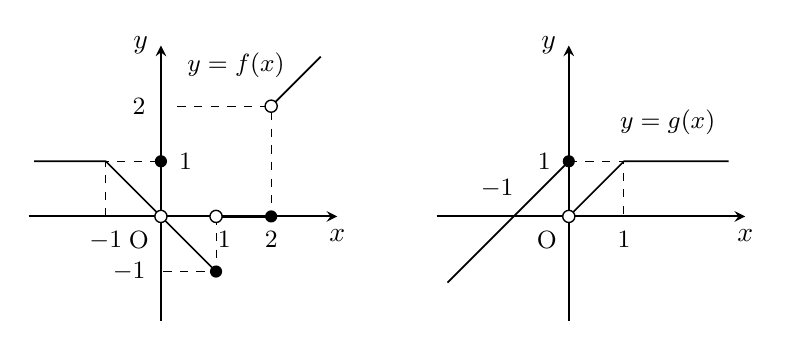
\begin{tikzpicture}[x=0.70cm, y=0.70cm, line width=0.5pt]
  % ── 왼쪽: y=f(x)
  \draw[->, >=stealth, line width=0.7pt] (-2.4,0) -- (3.2,0) node[below=1pt] {$x$};
  \draw[->, >=stealth, line width=0.7pt] (0,-1.9) -- (0,3.1) node[left=1pt] {$y$};
  \node[below=2pt, font=\small] at (-0.4,0) {$\pt{O}$};
  \draw[dashed, line width=0.35pt] (-1,0) -- (-1,1) -- (0,1);
  \draw[dashed, line width=0.35pt] (0.3,2) -- (2,2) -- (2,0);
  \draw[dashed, line width=0.35pt] (1,0) -- (1,-1) -- (0,-1);
  \draw[line width=0.6pt] (-2.3,1) -- (-1,1) -- (1,-1);
  % 이 조각은 x축 위에 그대로 놓이므로 축(0.7pt)보다 굵게 그려야 원문처럼 그래프로 보인다.
  \draw[line width=1.1pt] (1,0) -- (2,0);
  \draw[line width=0.6pt] (2,2) -- (2.9,2.9);
  \fill (0,1) circle (2.2pt);
  \fill (1,-1) circle (2.2pt);
  \fill (2,0) circle (2.2pt);
  \draw[fill=white, line width=0.5pt] (0,0) circle (2.2pt);
  \draw[fill=white, line width=0.5pt] (1,0) circle (2.2pt);
  \draw[fill=white, line width=0.5pt] (2,2) circle (2.2pt);
  \node[left=2pt, font=\small] at (0,2) {$2$};
  \node[right=3pt, font=\small] at (0,1) {$1$};
  \node[left=2pt, font=\small] at (0,-1) {$-1$};
  \node[below=2pt, font=\small] at (-1,0) {$-1$};
  \node[below=2pt, font=\small] at (1.15,0) {$1$};
  \node[below=2pt, font=\small] at (2,0) {$2$};
  \node[right=1pt, font=\small] at (0.25,2.75) {$y=f(x)$};
  % ── 오른쪽: y=g(x)
  \begin{scope}[xshift=5.18cm]
    \draw[->, >=stealth, line width=0.7pt] (-2.4,0) -- (3.2,0) node[below=1pt] {$x$};
    \draw[->, >=stealth, line width=0.7pt] (0,-1.9) -- (0,3.1) node[left=1pt] {$y$};
    \node[below=2pt, font=\small] at (-0.4,0) {$\pt{O}$};
    \draw[dashed, line width=0.35pt] (0,1) -- (1,1) -- (1,0);
    \draw[line width=0.6pt] (-2.2,-1.2) -- (0,1);
    \draw[line width=0.6pt] (0,0) -- (1,1) -- (2.9,1);
    \fill (0,1) circle (2.2pt);
    \draw[fill=white, line width=0.5pt] (0,0) circle (2.2pt);
    \node[left=3pt, font=\small] at (0,1) {$1$};
    \node[above=2pt, font=\small] at (-1.3,0.05) {$-1$};
    \node[below=2pt, font=\small] at (1,0) {$1$};
    \node[right=1pt, font=\small] at (0.7,1.7) {$y=g(x)$};
  \end{scope}
\end{tikzpicture}
}\end{center}
\noindent \bogi{ㄱ. $\displaystyle\lim_{x\to 0} f(x)$ \qquad ㄴ. $\displaystyle\lim_{x\to 0} f(g(x))$\\[1mm] ㄷ. $\displaystyle\lim_{x\to 0} g(f(x))$}
\dmchoicesauto{}{ㄱ}{ㄴ}{ㄱ, ㄴ}{ㄱ, ㄷ}{ㄱ, ㄴ, ㄷ}
}\vspace{8mm}
\vspace{3mm}\setcounter{dmproblemcount}{17}\dmpnum{10-18}{% id: 10-18
% book: 쎈B 미적분1 · 01 함수의 극한
% section: 유형 04 합성함수의 극한
% figure: tikz:fig-10-18
% answer: 
% answer_source: 
% variant_level: 0 (원본 전사)
% 이 파일은 build.mjs 가 items.json 에서 만든다. 고칠 때는 items.json 을 고친다.
\smash{\raisebox{4.5mm}{\dmkichul{쎈B 미적분1 10쪽 18번 · 서술형}}}
\noindent\begin{minipage}[t]{0.58\linewidth}\vspace{0pt}\raggedright 함수 $y=f(x)$의 그래프가 오른쪽 그림과 같을 때, $\displaystyle\lim_{t\to\infty} f\left(\dfrac{3t-1}{t-1}\right)+2\lim_{t\to\infty} f\left(\dfrac{2t+1}{t+1}\right)$의 값을 구하시오.\end{minipage}\hfill\begin{minipage}[t]{0.4\linewidth}\vspace{0pt}\centering \resizebox{\ifdim\width>\linewidth\linewidth\else\width\fi}{!}{% 10-18(10쪽) — 함수 y=f(x) 의 그래프(왼쪽 내리막 직선 · 곡선 · 수평선분 · 오른쪽 내리막 직선). 스캔 화질이 낮아 TikZ 로 다시 그림.
% 원문에 있는 것만: 눈금 숫자 2 3 (x) · 1 2 3 (y) · 라벨 O, x, y, y=f(x) · 좌표 안내 파선.
% 곡선은 원문 모양 그대로 지나는 점들을 재서 smooth 로 잇는다(식이 주어진 그래프가 아니다).
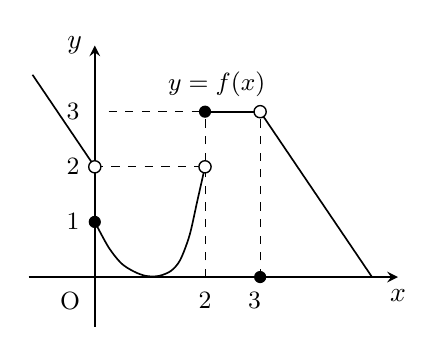
\begin{tikzpicture}[x=0.70cm, y=0.70cm, line width=0.5pt]
  \draw[->, >=stealth, line width=0.7pt] (-1.2,0) -- (5.5,0) node[below=1pt] {$x$};
  \draw[->, >=stealth, line width=0.7pt] (0,-0.9) -- (0,4.2) node[left=1pt] {$y$};
  \node[below=2pt, font=\small] at (-0.45,0) {$\pt{O}$};
  % 좌표 안내 파선(원문)
  \draw[dashed, line width=0.35pt] (0.25,3) -- (2,3);
  \draw[dashed, line width=0.35pt] (0,2) -- (2,2);
  \draw[dashed, line width=0.35pt] (2,0) -- (2,3);
  \draw[dashed, line width=0.35pt] (3,0) -- (3,3);
  % 그래프
  \draw[line width=0.6pt] (-1.13,3.67) -- (0,2);
  \draw[line width=0.6pt, smooth] plot coordinates {(0,1) (0.25,0.54) (0.48,0.25) (0.71,0.10) (0.93,0.02) (1.16,0.02) (1.38,0.11) (1.55,0.31) (1.72,0.76) (1.86,1.38) (2,2)};
  \draw[line width=0.6pt] (2,3) -- (3,3);
  \draw[line width=0.6pt] (3,3) -- (5.03,0);
  % 닫힌점
  \fill (0,1) circle (2.2pt);
  \fill (2,3) circle (2.2pt);
  \fill (3,0) circle (2.2pt);
  % 열린점
  \draw[fill=white, line width=0.5pt] (0,2) circle (2.2pt);
  \draw[fill=white, line width=0.5pt] (2,2) circle (2.2pt);
  \draw[fill=white, line width=0.5pt] (3,3) circle (2.2pt);
  % 눈금 라벨(원문 자리 그대로: y 눈금은 모두 축 왼쪽)
  \node[left=2pt, font=\small] at (0,3) {$3$};
  \node[left=2pt, font=\small] at (0,2) {$2$};
  \node[left=2pt, font=\small] at (0,1) {$1$};
  \node[below=2pt, font=\small] at (2,0) {$2$};
  \node[below=2pt, font=\small] at (2.9,0) {$3$};
  \node[right=1pt, font=\small] at (1.1,3.5) {$y=f(x)$};
\end{tikzpicture}
}\end{minipage}\par
}\vspace{8mm}
\dmsection{유형 05 함수의 극한에 대한 성질}
\vspace{3mm}\setcounter{dmproblemcount}{18}\dmpnum{10-19}{% id: 10-19
% book: 쎈B 미적분1 · 01 함수의 극한
% section: 유형 05 함수의 극한에 대한 성질
% figure: none
% answer: 
% answer_source: 
% variant_level: 0 (원본 전사)
% 이 파일은 build.mjs 가 items.json 에서 만든다. 고칠 때는 items.json 을 고친다.
\smash{\raisebox{4.5mm}{\dmkichul{쎈B 미적분1 10쪽 19번 · 대표 문제}}}
두 함수 $f(x)$, $g(x)$에 대하여\par\smallskip\dispeq{$\displaystyle\lim_{x\to a} f(x)=\infty$, $\displaystyle\lim_{x\to a}\{f(x)-g(x)\}=5$}\par\smallskip\noindent 일 때, $\displaystyle\lim_{x\to a}\dfrac{3f(x)-2g(x)}{-2f(x)+g(x)}$의 값은?
\dmchoicesauto{\rule[-3ex]{0pt}{8ex}}{$-\dfrac{3}{2}$}{$-1$}{$0$}{$1$}{$\dfrac{3}{2}$}
}\vspace{8mm}
\vspace{3mm}\setcounter{dmproblemcount}{19}\dmpnum{10-20}{% id: 10-20
% book: 쎈B 미적분1 · 01 함수의 극한
% section: 유형 05 함수의 극한에 대한 성질
% figure: none
% answer: 
% answer_source: 
% variant_level: 0 (원본 전사)
% 이 파일은 build.mjs 가 items.json 에서 만든다. 고칠 때는 items.json 을 고친다.
\smash{\raisebox{4.5mm}{\dmkichul{쎈B 미적분1 10쪽 20번}}}
함수 $f(x)$에 대하여 $\displaystyle\lim_{x\to 5}(x-5)f(x)=2$일 때, $\displaystyle\lim_{x\to 5}(x^2-4x-5)f(x)$의 값을 구하시오.
}\vspace{8mm}
\vspace{3mm}\setcounter{dmproblemcount}{20}\dmpnum{10-21}{% id: 10-21
% book: 쎈B 미적분1 · 01 함수의 극한
% section: 유형 05 함수의 극한에 대한 성질
% figure: none
% answer: 
% answer_source: 
% variant_level: 0 (원본 전사)
% 이 파일은 build.mjs 가 items.json 에서 만든다. 고칠 때는 items.json 을 고친다.
\smash{\raisebox{4.5mm}{\dmkichul{쎈B 미적분1 10쪽 21번}}}
함수 $f(x)$에 대하여 $\displaystyle\lim_{x\to\infty}\dfrac{1}{x^2}\{f(x)+3x^2\}=0$일 때, $\displaystyle\lim_{x\to\infty}\dfrac{2f(x)-4x+1}{3f(x)+x}$의 값은?
\dmchoicesauto{\rule[-3ex]{0pt}{8ex}}{$-1$}{$-\dfrac{2}{3}$}{$\dfrac{1}{3}$}{$\dfrac{2}{3}$}{$1$}
}\vspace{8mm}
\vspace{3mm}\setcounter{dmproblemcount}{21}\dmpnum{10-22}{% id: 10-22
% book: 쎈B 미적분1 · 01 함수의 극한
% section: 유형 05 함수의 극한에 대한 성질
% figure: none
% answer: 
% answer_source: 
% variant_level: 0 (원본 전사)
% 이 파일은 build.mjs 가 items.json 에서 만든다. 고칠 때는 items.json 을 고친다.
\smash{\raisebox{4.5mm}{\dmkichul{쎈B 미적분1 10쪽 22번 · 서술형}}}
두 함수 $f(x)$, $g(x)$에 대하여\par\smallskip\dispeq{$\displaystyle\lim_{x\to\infty} f(x)=6$, $\displaystyle\lim_{x\to\infty}\{2f(x)-3g(x)\}=24$}\par\smallskip\noindent 일 때, $\displaystyle\lim_{x\to\infty} g(x)$의 값을 구하시오.
}\vspace{8mm}
\vspace{3mm}\setcounter{dmproblemcount}{22}\dmpnum{10-23}{% id: 10-23
% book: 쎈B 미적분1 · 01 함수의 극한
% section: 유형 05 함수의 극한에 대한 성질
% figure: none
% answer: 
% answer_source: 
% variant_level: 0 (원본 전사)
% 이 파일은 build.mjs 가 items.json 에서 만든다. 고칠 때는 items.json 을 고친다.
\smash{\raisebox{4.5mm}{\dmkichul{쎈B 미적분1 10쪽 23번}}}
두 함수 $f(x)$, $g(x)$에 대하여 $\displaystyle\lim_{x\to -1} f(x)=\alpha$, $\displaystyle\lim_{x\to -1} g(x)=\beta$이고\par\smallskip\dispeq{$\displaystyle\lim_{x\to -1}\{f(x)+g(x)\}=5$, $\displaystyle\lim_{x\to -1} f(x)g(x)=-14$}\par\smallskip\noindent 일 때, $\displaystyle\lim_{x\to -1}\dfrac{-2g(x)+3}{f(x)+1}$의 값은? \dmcondfill{$\alpha<\beta$}{}
\dmchoicesauto{}{$9$}{$10$}{$11$}{$12$}{$13$}
}\vspace{8mm}
\vspace{3mm}\setcounter{dmproblemcount}{23}\dmpnum{11-24}{% id: 11-24
% book: 쎈B 미적분1 · 01 함수의 극한
% section: 유형 05 함수의 극한에 대한 성질
% figure: none
% answer: 
% answer_source: 
% variant_level: 0 (원본 전사)
% 이 파일은 build.mjs 가 items.json 에서 만든다. 고칠 때는 items.json 을 고친다.
\smash{\raisebox{4.5mm}{\dmkichul{쎈B 미적분1 11쪽 24번}}}
함수의 극한에 대한 설명으로 옳은 것만을 보기에서 있는 대로 고르시오. \dmcondfill{$a$는 실수이다.}{} \bogi{ㄱ. $\displaystyle\lim_{x\to a}\{f(x)-g(x)\}=0$이면 $\displaystyle\lim_{x\to a} f(x)=\lim_{x\to a} g(x)$이다.\\ ㄴ. $\displaystyle\lim_{x\to\infty} f(x)$와 $\displaystyle\lim_{x\to\infty}\dfrac{g(x)}{f(x)}$의 값이 각각 존재하면 $\displaystyle\lim_{x\to\infty} g(x)$의 값도 존재한다.\\ ㄷ. $\displaystyle\lim_{x\to a} f(x)g(x)$와 $\displaystyle\lim_{x\to a} g(x)$의 값이 각각 존재하고 $\displaystyle\lim_{x\to a} g(x)\ne 0$이면 $\displaystyle\lim_{x\to a} f(x)$의 값이 존재한다.\\ ㄹ. $\displaystyle\lim_{x\to a}(x-a)f(x)$와 $\displaystyle\lim_{x\to a}\dfrac{g(x)}{x-a}$의 값이 각각 존재하면 $\displaystyle\lim_{x\to a} f(x)g(x)$의 값도 존재한다.}
}\vspace{8mm}
\dmsection{유형 06 $\frac{0}{0}$ 꼴의 극한; 유리식}
\vspace{3mm}\setcounter{dmproblemcount}{24}\dmpnum{11-25}{% id: 11-25
% book: 쎈B 미적분1 · 01 함수의 극한
% section: 유형 06 $\frac{0}{0}$ 꼴의 극한; 유리식
% figure: none
% answer: 
% answer_source: 
% variant_level: 0 (원본 전사)
% 이 파일은 build.mjs 가 items.json 에서 만든다. 고칠 때는 items.json 을 고친다.
\smash{\raisebox{4.5mm}{\dmkichul{쎈B 미적분1 11쪽 25번 · 대표 문제}}}
$\displaystyle\lim_{x\to-2}\dfrac{x^3+x^2-x+2}{x^2+x-2}$의 값을 구하시오.
}\vspace{8mm}
\vspace{3mm}\setcounter{dmproblemcount}{25}\dmpnum{11-26}{% id: 11-26
% book: 쎈B 미적분1 · 01 함수의 극한
% section: 유형 06 $\frac{0}{0}$ 꼴의 극한; 유리식
% figure: none
% answer: 
% answer_source: 
% variant_level: 0 (원본 전사)
% 이 파일은 build.mjs 가 items.json 에서 만든다. 고칠 때는 items.json 을 고친다.
\smash{\raisebox{4.5mm}{\dmkichul{쎈B 미적분1 11쪽 26번}}}
다항함수 $f(x)$에 대하여 $\displaystyle\lim_{x\to 2}\dfrac{x^2-4}{(x^4-16)f(x)}=-1$일 때, $f(2)$의 값을 구하시오. \dmcondfill{$f(x)\ne 0$}{}
}\vspace{8mm}
\vspace{3mm}\setcounter{dmproblemcount}{26}\dmpnum{11-27}{% id: 11-27
% book: 쎈B 미적분1 · 01 함수의 극한
% section: 유형 06 $\frac{0}{0}$ 꼴의 극한; 유리식
% figure: none
% answer: 
% answer_source: 
% variant_level: 0 (원본 전사)
% 이 파일은 build.mjs 가 items.json 에서 만든다. 고칠 때는 items.json 을 고친다.
\smash{\raisebox{4.5mm}{\dmkichul{쎈B 미적분1 11쪽 27번}}}
다항함수 $f(x)$에 대하여 $\displaystyle\lim_{x\to 1}\dfrac{f(x)+3}{x-1}=8$일 때, $\displaystyle\lim_{x\to 1}\dfrac{\{f(x)\}^2+3f(x)}{x^2f(x)-f(x)}$의 값은? \dmcondfill{$f(x)\ne 0$}{}
\dmchoicesauto{\rule[-3ex]{0pt}{8ex}}{$-4$}{$-2$}{$\dfrac{1}{2}$}{$2$}{$4$}
}\vspace{8mm}
\vspace{3mm}\setcounter{dmproblemcount}{27}\dmpnum{11-28}{% id: 11-28
% book: 쎈B 미적분1 · 01 함수의 극한
% section: 유형 06 $\frac{0}{0}$ 꼴의 극한; 유리식
% figure: none
% answer: 
% answer_source: 
% variant_level: 0 (원본 전사)
% 이 파일은 build.mjs 가 items.json 에서 만든다. 고칠 때는 items.json 을 고친다.
\smash{\raisebox{4.5mm}{\dmkichul{쎈B 미적분1 11쪽 28번 · 서술형}}}
$\displaystyle\lim_{x\to 1-}\dfrac{2x^2-x-1}{|x^2-1|}=a$, $\displaystyle\lim_{x\to 0+}\dfrac{x}{x+|3x|}=b$라 할 때, 실수 $a$, $b$에 대하여 $\dfrac{a}{b}$의 값을 구하시오.
}\vspace{8mm}
\vspace{3mm}\setcounter{dmproblemcount}{28}\dmpnum{11-29}{% id: 11-29
% book: 쎈B 미적분1 · 01 함수의 극한
% section: 유형 06 $\frac{0}{0}$ 꼴의 극한; 유리식
% figure: none
% answer: 
% answer_source: 
% variant_level: 0 (원본 전사)
% 이 파일은 build.mjs 가 items.json 에서 만든다. 고칠 때는 items.json 을 고친다.
\smash{\raisebox{4.5mm}{\dmkichul{쎈B 미적분1 11쪽 29번}}}
함수 $f(x)=2x^3+3x$의 역함수를 $f^{-1}(x)$라 하자. $\displaystyle\lim_{x\to 0}\dfrac{f^{-1}(x)}{4x}=\dfrac{p}{q}$일 때, $pq$의 값은? \dmcondfill{$p$, $q$는 서로소인 자연수이다.}{}
\dmchoicesauto{}{$5$}{$8$}{$10$}{$12$}{$15$}
}\vspace{8mm}
\dmsection{유형 07 $\frac{0}{0}$ 꼴의 극한; 무리식}
\vspace{3mm}\setcounter{dmproblemcount}{29}\dmpnum{12-30}{% id: 12-30
% book: 쎈B 미적분1 · 01 함수의 극한
% section: 유형 07 $\frac{0}{0}$ 꼴의 극한; 무리식
% figure: none
% answer: 
% answer_source: 
% variant_level: 0 (원본 전사)
% 이 파일은 build.mjs 가 items.json 에서 만든다. 고칠 때는 items.json 을 고친다.
\smash{\raisebox{4.5mm}{\dmkichul{쎈B 미적분1 12쪽 30번 · 대표 문제}}}
$\displaystyle\lim_{x\to 3}\dfrac{x^2-4x+3}{\sqrt{x+1}-2}$의 값을 구하시오.
}\vspace{8mm}
\vspace{3mm}\setcounter{dmproblemcount}{30}\dmpnum{12-31}{% id: 12-31
% book: 쎈B 미적분1 · 01 함수의 극한
% section: 유형 07 $\frac{0}{0}$ 꼴의 극한; 무리식
% figure: none
% answer: 
% answer_source: 
% variant_level: 0 (원본 전사)
% 이 파일은 build.mjs 가 items.json 에서 만든다. 고칠 때는 items.json 을 고친다.
\smash{\raisebox{4.5mm}{\dmkichul{쎈B 미적분1 12쪽 31번}}}
함수 $f(x)$에 대하여 $\displaystyle\lim_{x\to 1} f(x)=2$일 때, $\displaystyle\lim_{x\to 1}\dfrac{(x-1)f(x)}{\sqrt{x}-1}$의 값은?
\dmchoicesauto{}{$1$}{$2$}{$4$}{$6$}{$8$}
}\vspace{8mm}
\vspace{3mm}\setcounter{dmproblemcount}{31}\dmpnum{12-32}{% id: 12-32
% book: 쎈B 미적분1 · 01 함수의 극한
% section: 유형 07 $\frac{0}{0}$ 꼴의 극한; 무리식
% figure: none
% answer: 
% answer_source: 
% variant_level: 0 (원본 전사)
% 이 파일은 build.mjs 가 items.json 에서 만든다. 고칠 때는 items.json 을 고친다.
\smash{\raisebox{4.5mm}{\dmkichul{쎈B 미적분1 12쪽 32번}}}
함수 $f(x)$에 대하여 $\displaystyle\lim_{x\to 0} f(x)=\dfrac{1}{3}$일 때, $\displaystyle\lim_{x\to 0}\dfrac{\sqrt{1+2xf(x)}-\sqrt{1-2xf(x)}}{x}$의 값을 구하시오.
}\vspace{8mm}
\vspace{3mm}\setcounter{dmproblemcount}{32}\dmpnum{12-33}{% id: 12-33
% book: 쎈B 미적분1 · 01 함수의 극한
% section: 유형 07 $\frac{0}{0}$ 꼴의 극한; 무리식
% figure: none
% answer: 
% answer_source: 
% variant_level: 0 (원본 전사)
% 이 파일은 build.mjs 가 items.json 에서 만든다. 고칠 때는 items.json 을 고친다.
\smash{\raisebox{4.5mm}{\dmkichul{쎈B 미적분1 12쪽 33번}}}
$\displaystyle\lim_{x\to 0}\dfrac{\sqrt{3-2x}-\sqrt{3+x}}{\sqrt{4-2x}-\sqrt{4-x}}$의 값을 구하시오.
}\vspace{8mm}
\dmsection{유형 08 $\frac{\infty}{\infty}$ 꼴의 극한}
\vspace{3mm}\setcounter{dmproblemcount}{33}\dmpnum{12-34}{% id: 12-34
% book: 쎈B 미적분1 · 01 함수의 극한
% section: 유형 08 $\frac{\infty}{\infty}$ 꼴의 극한
% figure: none
% answer: 
% answer_source: 
% variant_level: 0 (원본 전사)
% 이 파일은 build.mjs 가 items.json 에서 만든다. 고칠 때는 items.json 을 고친다.
\smash{\raisebox{4.5mm}{\dmkichul{쎈B 미적분1 12쪽 34번 · 대표 문제}}}
$\displaystyle\lim_{x\to-\infty}\dfrac{\sqrt{9x^2+1}-x}{\sqrt{x^2-5x+1}+2x}$의 값은?
\dmchoicesauto{\rule[-3ex]{0pt}{8ex}}{$-4$}{$-2$}{$-\dfrac{1}{2}$}{$2$}{$4$}
}\vspace{8mm}
\vspace{3mm}\setcounter{dmproblemcount}{34}\dmpnum{12-35}{% id: 12-35
% book: 쎈B 미적분1 · 01 함수의 극한
% section: 유형 08 $\frac{\infty}{\infty}$ 꼴의 극한
% figure: none
% answer: 
% answer_source: 
% variant_level: 0 (원본 전사)
% 이 파일은 build.mjs 가 items.json 에서 만든다. 고칠 때는 items.json 을 고친다.
\smash{\raisebox{4.5mm}{\dmkichul{쎈B 미적분1 12쪽 35번}}}
$\displaystyle\lim_{x\to\infty}\dfrac{2x-1}{\sqrt{x^2+1}+\sqrt{9x^2+x}}$의 값을 구하시오.
}\vspace{8mm}
\vspace{3mm}\setcounter{dmproblemcount}{35}\dmpnum{12-36}{% id: 12-36
% book: 쎈B 미적분1 · 01 함수의 극한
% section: 유형 08 $\frac{\infty}{\infty}$ 꼴의 극한
% figure: none
% answer: 
% answer_source: 
% variant_level: 0 (원본 전사)
% 이 파일은 build.mjs 가 items.json 에서 만든다. 고칠 때는 items.json 을 고친다.
\smash{\raisebox{4.5mm}{\dmkichul{쎈B 미적분1 12쪽 36번}}}
$\displaystyle\lim_{x\to\infty}\dfrac{2x+3}{x^2-1}=a$, $\displaystyle\lim_{x\to\infty}\dfrac{5x^2-x}{2x^2+1}=b$, $\displaystyle\lim_{x\to\infty}\dfrac{6x}{1-\sqrt{16x^2+3}}=c$라 할 때, 실수 $a$, $b$, $c$에 대하여 다음 중 옳은 것은?
\dmchoicesauto{}{$a>b$}{$a=c$}{$b<c$}{$a-b=c$}{$a+b+c=1$}
}\vspace{8mm}
\vspace{3mm}\setcounter{dmproblemcount}{36}\dmpnum{13-37}{% id: 13-37
% book: 쎈B 미적분1 · 01 함수의 극한
% section: 유형 08 $\frac{\infty}{\infty}$ 꼴의 극한
% figure: none
% answer: 
% answer_source: 
% variant_level: 0 (원본 전사)
% 이 파일은 build.mjs 가 items.json 에서 만든다. 고칠 때는 items.json 을 고친다.
\smash{\raisebox{4.5mm}{\dmkichul{쎈B 미적분1 13쪽 37번}}}
$\displaystyle\lim_{x\to\infty}\dfrac{f(x)}{x}=1$일 때, $\displaystyle\lim_{x\to\infty}\dfrac{3x^2-\{f(x)\}^2}{x^2+2f(x)}$의 값을 구하시오.
}\vspace{8mm}
\vspace{3mm}\setcounter{dmproblemcount}{37}\dmpnum{13-38}{% id: 13-38
% book: 쎈B 미적분1 · 01 함수의 극한
% section: 유형 08 $\frac{\infty}{\infty}$ 꼴의 극한
% figure: none
% answer: 
% answer_source: 
% variant_level: 0 (원본 전사)
% 이 파일은 build.mjs 가 items.json 에서 만든다. 고칠 때는 items.json 을 고친다.
\smash{\raisebox{4.5mm}{\dmkichul{쎈B 미적분1 13쪽 38번 · 서술형}}}
$\displaystyle\lim_{x\to-\infty}\dfrac{f(x)}{x}=a$, $\displaystyle\lim_{x\to-\infty}\dfrac{3f(x)+\sqrt{f(x)+4x^2}}{f(x)}=2$일 때, 실수 $a$의 값을 구하시오.
}\vspace{8mm}
\dmsection{유형 09 $\infty-\infty$ 꼴의 극한}
\vspace{3mm}\setcounter{dmproblemcount}{38}\dmpnum{13-39}{% id: 13-39
% book: 쎈B 미적분1 · 01 함수의 극한
% section: 유형 09 $\infty-\infty$ 꼴의 극한
% figure: none
% answer: 
% answer_source: 
% variant_level: 0 (원본 전사)
% 이 파일은 build.mjs 가 items.json 에서 만든다. 고칠 때는 items.json 을 고친다.
\smash{\raisebox{4.5mm}{\dmkichul{쎈B 미적분1 13쪽 39번 · 대표 문제}}}
$\displaystyle\lim_{x\to-\infty}(\sqrt{2-6x+x^2}+x)$의 값은?
\dmchoicesauto{}{$-3$}{$-2$}{$1$}{$2$}{$3$}
}\vspace{8mm}
\vspace{3mm}\setcounter{dmproblemcount}{39}\dmpnum{13-40}{% id: 13-40
% book: 쎈B 미적분1 · 01 함수의 극한
% section: 유형 09 $\infty-\infty$ 꼴의 극한
% figure: none
% answer: 
% answer_source: 
% variant_level: 0 (원본 전사)
% 이 파일은 build.mjs 가 items.json 에서 만든다. 고칠 때는 items.json 을 고친다.
\smash{\raisebox{4.5mm}{\dmkichul{쎈B 미적분1 13쪽 40번}}}
$\displaystyle\lim_{x\to\infty}\dfrac{1}{\sqrt{4x^2-x+5}-2x}$의 값을 구하시오.
}\vspace{8mm}
\vspace{3mm}\setcounter{dmproblemcount}{40}\dmpnum{13-41}{% id: 13-41
% book: 쎈B 미적분1 · 01 함수의 극한
% section: 유형 09 $\infty-\infty$ 꼴의 극한
% figure: none
% answer: 
% answer_source: 
% variant_level: 0 (원본 전사)
% 이 파일은 build.mjs 가 items.json 에서 만든다. 고칠 때는 items.json 을 고친다.
\smash{\raisebox{4.5mm}{\dmkichul{쎈B 미적분1 13쪽 41번 · 서술형}}}
\dispeq{$\displaystyle\lim_{x\to-4}\dfrac{\sqrt{x+5}-1}{x+4}=p$, $\displaystyle\lim_{x\to\infty}(\sqrt{x^2+3x-2}-\sqrt{x^2-x+2})=q$}\par\smallskip\noindent 라 할 때, 실수 $p$, $q$에 대하여 $2p+q$의 값을 구하시오.
}\vspace{8mm}
\vspace{3mm}\setcounter{dmproblemcount}{41}\dmpnum{13-42}{% id: 13-42
% book: 쎈B 미적분1 · 01 함수의 극한
% section: 유형 09 $\infty-\infty$ 꼴의 극한
% figure: none
% answer: 
% answer_source: 
% variant_level: 0 (원본 전사)
% 이 파일은 build.mjs 가 items.json 에서 만든다. 고칠 때는 items.json 을 고친다.
\smash{\raisebox{4.5mm}{\dmkichul{쎈B 미적분1 13쪽 42번}}}
$\displaystyle\lim_{x\to\infty}(\sqrt{x^2-2[x]}-x)$의 값은? \dmcondfill{$[x]$는 $x$보다 크지 않은 최대의 정수이다.}{}
\dmchoicesauto{}{$-2$}{$-1$}{$0$}{$1$}{$2$}
}\vspace{8mm}
\dmsection{유형 10 $\infty\times 0$ 꼴의 극한}
\vspace{3mm}\setcounter{dmproblemcount}{42}\dmpnum{13-43}{% id: 13-43
% book: 쎈B 미적분1 · 01 함수의 극한
% section: 유형 10 $\infty\times 0$ 꼴의 극한
% figure: none
% answer: 
% answer_source: 
% variant_level: 0 (원본 전사)
% 이 파일은 build.mjs 가 items.json 에서 만든다. 고칠 때는 items.json 을 고친다.
\smash{\raisebox{4.5mm}{\dmkichul{쎈B 미적분1 13쪽 43번 · 대표 문제}}}
$\displaystyle\lim_{x\to 1}\dfrac{1}{x-1}\Big\{\dfrac{1}{(x+1)^2}-\dfrac{1}{4}\Big\}$의 값을 구하시오.
}\vspace{8mm}
\vspace{3mm}\setcounter{dmproblemcount}{43}\dmpnum{14-44}{% id: 14-44
% book: 쎈B 미적분1 · 01 함수의 극한
% section: 유형 10 $\infty\times 0$ 꼴의 극한
% figure: none
% answer: 
% answer_source: 
% variant_level: 0 (원본 전사)
% 이 파일은 build.mjs 가 items.json 에서 만든다. 고칠 때는 items.json 을 고친다.
\smash{\raisebox{4.5mm}{\dmkichul{쎈B 미적분1 14쪽 44번}}}
$\displaystyle\lim_{x\to 9}(\sqrt{x}-3)\Big(1+\dfrac{2}{x-9}\Big)$의 값은?
\dmchoicesauto{\rule[-3ex]{0pt}{8ex}}{$\dfrac{1}{6}$}{$\dfrac{1}{3}$}{$\dfrac{1}{2}$}{$\dfrac{2}{3}$}{$\dfrac{5}{6}$}
}\vspace{8mm}
\vspace{3mm}\setcounter{dmproblemcount}{44}\dmpnum{14-45}{% id: 14-45
% book: 쎈B 미적분1 · 01 함수의 극한
% section: 유형 10 $\infty\times 0$ 꼴의 극한
% figure: none
% answer: 
% answer_source: 
% variant_level: 0 (원본 전사)
% 이 파일은 build.mjs 가 items.json 에서 만든다. 고칠 때는 items.json 을 고친다.
\smash{\raisebox{4.5mm}{\dmkichul{쎈B 미적분1 14쪽 45번}}}
함수 $f(x)=x^2-2x+1$에 대하여 $\displaystyle\lim_{n\to\infty} n^2\Big\{f\Big(\dfrac{2}{n}+3\Big)-f(3)\Big\}^2$의 값을 구하시오.
}\vspace{8mm}
\dmsection{유형 11 미정계수의 결정 (1)}
\vspace{3mm}\setcounter{dmproblemcount}{45}\dmpnum{14-46}{% id: 14-46
% book: 쎈B 미적분1 · 01 함수의 극한
% section: 유형 11 미정계수의 결정 (1)
% figure: none
% answer: 
% answer_source: 
% variant_level: 0 (원본 전사)
% 이 파일은 build.mjs 가 items.json 에서 만든다. 고칠 때는 items.json 을 고친다.
\smash{\raisebox{4.5mm}{\dmkichul{쎈B 미적분1 14쪽 46번 · 대표 문제}}}
$\displaystyle\lim_{x\to-3}\dfrac{x^2+ax+b}{x+3}=-2$일 때, 상수 $a$, $b$에 대하여 $a+b$의 값은?
\dmchoicesauto{}{$5$}{$7$}{$9$}{$11$}{$13$}
}\vspace{8mm}
\vspace{3mm}\setcounter{dmproblemcount}{46}\dmpnum{14-47}{% id: 14-47
% book: 쎈B 미적분1 · 01 함수의 극한
% section: 유형 11 미정계수의 결정 (1)
% figure: none
% answer: 
% answer_source: 
% variant_level: 0 (원본 전사)
% 이 파일은 build.mjs 가 items.json 에서 만든다. 고칠 때는 items.json 을 고친다.
\smash{\raisebox{4.5mm}{\dmkichul{쎈B 미적분1 14쪽 47번 · 서술형}}}
함수 $f(x)=2x^3+ax^2+b$에 대하여 $\displaystyle\lim_{x\to-1}\dfrac{f(x)}{x+1}=12$일 때, $f(-2)$의 값을 구하시오. \dmcondfill{$a$, $b$는 상수이다.}{}
}\vspace{8mm}
\vspace{3mm}\setcounter{dmproblemcount}{47}\dmpnum{14-48}{% id: 14-48
% book: 쎈B 미적분1 · 01 함수의 극한
% section: 유형 11 미정계수의 결정 (1)
% figure: none
% answer: 
% answer_source: 
% variant_level: 0 (원본 전사)
% 이 파일은 build.mjs 가 items.json 에서 만든다. 고칠 때는 items.json 을 고친다.
\smash{\raisebox{4.5mm}{\dmkichul{쎈B 미적분1 14쪽 48번}}}
$\displaystyle\lim_{x\to 3}\dfrac{3\sqrt{16+x^2}-5x}{ax+b}=8$일 때, 상수 $a$, $b$에 대하여 $b-a$의 값은?
\dmchoicesauto{\rule[-3ex]{0pt}{8ex}}{$-\dfrac{16}{5}$}{$-\dfrac{8}{5}$}{$-\dfrac{1}{5}$}{$\dfrac{8}{5}$}{$\dfrac{16}{5}$}
}\vspace{8mm}
\vspace{3mm}\setcounter{dmproblemcount}{48}\dmpnum{14-49}{% id: 14-49
% book: 쎈B 미적분1 · 01 함수의 극한
% section: 유형 11 미정계수의 결정 (1)
% figure: none
% answer: 
% answer_source: 
% variant_level: 0 (원본 전사)
% 이 파일은 build.mjs 가 items.json 에서 만든다. 고칠 때는 items.json 을 고친다.
\smash{\raisebox{4.5mm}{\dmkichul{쎈B 미적분1 14쪽 49번}}}
$\displaystyle\lim_{x\to 1}\dfrac{1}{x-1}\Big(\dfrac{1}{a}-\dfrac{1}{x+b}\Big)=\dfrac{1}{16}$일 때, 자연수 $a$, $b$에 대하여 $a+b$의 값은?
\dmchoicesauto{}{$7$}{$9$}{$11$}{$13$}{$15$}
}\vspace{8mm}
\vspace{3mm}\setcounter{dmproblemcount}{49}\dmpnum{15-50}{% id: 15-50
% book: 쎈B 미적분1 · 01 함수의 극한
% section: 유형 11 미정계수의 결정 (1)
% figure: none
% answer: 
% answer_source: 
% variant_level: 0 (원본 전사)
% 이 파일은 build.mjs 가 items.json 에서 만든다. 고칠 때는 items.json 을 고친다.
\smash{\raisebox{4.5mm}{\dmkichul{쎈B 미적분1 15쪽 50번}}}
$\displaystyle\lim_{x\to\infty}\dfrac{ax^2+bx+c}{x^2-2x-3}=5$, $\displaystyle\lim_{x\to-1}\dfrac{ax^2+bx+c}{x^2-2x-3}=\dfrac{3}{2}$일 때, 상수 $a$, $b$, $c$에 대하여 $abc$의 값은?
\dmchoicesauto{}{$-20$}{$-10$}{$0$}{$10$}{$20$}
}\vspace{8mm}
\dmsection{유형 12 미정계수의 결정 (2)}
\vspace{3mm}\setcounter{dmproblemcount}{50}\dmpnum{15-51}{% id: 15-51
% book: 쎈B 미적분1 · 01 함수의 극한
% section: 유형 12 미정계수의 결정 (2)
% figure: none
% answer: 
% answer_source: 
% variant_level: 0 (원본 전사)
% 이 파일은 build.mjs 가 items.json 에서 만든다. 고칠 때는 items.json 을 고친다.
\smash{\raisebox{4.5mm}{\dmkichul{쎈B 미적분1 15쪽 51번 · 대표 문제}}}
$\displaystyle\lim_{x\to-\infty}(\sqrt{ax^2+2bx}+2x)=-1$일 때, 상수 $a$, $b$에 대하여 $\dfrac{a}{b}$의 값을 구하시오.
}\vspace{8mm}
\vspace{3mm}\setcounter{dmproblemcount}{51}\dmpnum{15-52}{% id: 15-52
% book: 쎈B 미적분1 · 01 함수의 극한
% section: 유형 12 미정계수의 결정 (2)
% figure: none
% answer: 
% answer_source: 
% variant_level: 0 (원본 전사)
% 이 파일은 build.mjs 가 items.json 에서 만든다. 고칠 때는 items.json 을 고친다.
\smash{\raisebox{4.5mm}{\dmkichul{쎈B 미적분1 15쪽 52번}}}
$\displaystyle\lim_{x\to\infty}(\sqrt{x^2-ax+4}-\sqrt{x^2+3ax+1})=10$을 만족시키는 상수 $a$의 값은?
\dmchoicesauto{}{$-10$}{$-5$}{$0$}{$5$}{$10$}
}\vspace{8mm}
\vspace{3mm}\setcounter{dmproblemcount}{52}\dmpnum{15-53}{% id: 15-53
% book: 쎈B 미적분1 · 01 함수의 극한
% section: 유형 12 미정계수의 결정 (2)
% figure: none
% answer: 
% answer_source: 
% variant_level: 0 (원본 전사)
% 이 파일은 build.mjs 가 items.json 에서 만든다. 고칠 때는 items.json 을 고친다.
\smash{\raisebox{4.5mm}{\dmkichul{쎈B 미적분1 15쪽 53번 · 서술형}}}
$\displaystyle\lim_{x\to\infty}(\sqrt{ax^2+4x+1}-\sqrt{x^2-2ax+1})=b$를 만족시키는 실수 $a$, $b$에 대하여 $ab$의 값을 구하시오.
}\vspace{8mm}
\dmsection{유형 13 다항함수의 결정}
\vspace{3mm}\setcounter{dmproblemcount}{53}\dmpnum{15-54}{% id: 15-54
% book: 쎈B 미적분1 · 01 함수의 극한
% section: 유형 13 다항함수의 결정
% figure: none
% answer: 
% answer_source: 
% variant_level: 0 (원본 전사)
% 이 파일은 build.mjs 가 items.json 에서 만든다. 고칠 때는 items.json 을 고친다.
\smash{\raisebox{4.5mm}{\dmkichul{쎈B 미적분1 15쪽 54번 · 대표 문제}}}
다항함수 $f(x)$가\par\smallskip\dispeq{$\displaystyle\lim_{x\to\infty}\dfrac{f(x)}{2x^2+1}=1$, $\displaystyle\lim_{x\to-1}\dfrac{f(x)}{x^2-1}=-3$}\par\smallskip\noindent 을 만족시킬 때, $f(6)$의 값은?
\dmchoicesauto{}{$80$}{$100$}{$120$}{$140$}{$160$}
}\vspace{8mm}
\vspace{3mm}\setcounter{dmproblemcount}{54}\dmpnum{15-55}{% id: 15-55
% book: 쎈B 미적분1 · 01 함수의 극한
% section: 유형 13 다항함수의 결정
% figure: none
% answer: 
% answer_source: 
% variant_level: 0 (원본 전사)
% 이 파일은 build.mjs 가 items.json 에서 만든다. 고칠 때는 items.json 을 고친다.
\smash{\raisebox{4.5mm}{\dmkichul{쎈B 미적분1 15쪽 55번}}}
최고차항의 계수가 1인 이차함수 $f(x)$가 $\displaystyle\lim_{x\to 1}\dfrac{f(x)}{x-1}=7$을 만족시킬 때, $f(x)$를 구하시오.
}\vspace{8mm}
\vspace{3mm}\setcounter{dmproblemcount}{55}\dmpnum{16-56}{% id: 16-56
% book: 쎈B 미적분1 · 01 함수의 극한
% section: 유형 13 다항함수의 결정
% figure: none
% answer: 
% answer_source: 
% variant_level: 0 (원본 전사)
% 이 파일은 build.mjs 가 items.json 에서 만든다. 고칠 때는 items.json 을 고친다.
\smash{\raisebox{4.5mm}{\dmkichul{쎈B 미적분1 16쪽 56번}}}
다항함수 $f(x)$가 다음 조건을 모두 만족시킬 때, $f(x)$를 $x-1$로 나누었을 때의 나머지를 구하시오. \exprbox{㈎ $\displaystyle\lim_{x\to\infty}\dfrac{f(x)+2x^3}{x^2}=1$ \qquad ㈏ $\displaystyle\lim_{x\to 0}\dfrac{f(x)}{x}=2$}
}\vspace{8mm}
\vspace{3mm}\setcounter{dmproblemcount}{56}\dmpnum{16-57}{% id: 16-57
% book: 쎈B 미적분1 · 01 함수의 극한
% section: 유형 13 다항함수의 결정
% figure: none
% answer: 
% answer_source: 
% variant_level: 0 (원본 전사)
% 이 파일은 build.mjs 가 items.json 에서 만든다. 고칠 때는 items.json 을 고친다.
\smash{\raisebox{4.5mm}{\dmkichul{쎈B 미적분1 16쪽 57번}}}
다항함수 $f(x)$가\par\smallskip\dispeq{$\displaystyle\lim_{x\to\infty}\dfrac{f(x)-3x^2}{4x-1}=a$, $\displaystyle\lim_{x\to-2}\dfrac{f(x)}{x+2}=6$}\par\smallskip\noindent 을 만족시킬 때, 실수 $a$의 값은? \dmcondfill{$a\ne 0$}{}
\dmchoicesauto{\rule[-3ex]{0pt}{8ex}}{$-6$}{$-\dfrac{9}{2}$}{$-3$}{$3$}{$\dfrac{9}{2}$}
}\vspace{8mm}
\vspace{3mm}\setcounter{dmproblemcount}{57}\dmpnum{16-58}{% id: 16-58
% book: 쎈B 미적분1 · 01 함수의 극한
% section: 유형 13 다항함수의 결정
% figure: none
% answer: 
% answer_source: 
% variant_level: 0 (원본 전사)
% 이 파일은 build.mjs 가 items.json 에서 만든다. 고칠 때는 items.json 을 고친다.
\smash{\raisebox{4.5mm}{\dmkichul{쎈B 미적분1 16쪽 58번}}}
다항함수 $f(x)$가 $\displaystyle\lim_{x\to 5}\dfrac{f(x)-x^2}{x-5}=2$를 만족시킬 때, 함수 $g(x)=f(x)-f(5)$에 대하여 $\displaystyle\lim_{x\to 5}\dfrac{f(x)g(x)}{x^2-25}$의 값을 구하시오.
}\vspace{8mm}
\dmsection{유형 14 함수의 극한의 대소 관계}
\vspace{3mm}\setcounter{dmproblemcount}{58}\dmpnum{16-59}{% id: 16-59
% book: 쎈B 미적분1 · 01 함수의 극한
% section: 유형 14 함수의 극한의 대소 관계
% figure: none
% answer: 
% answer_source: 
% variant_level: 0 (원본 전사)
% 이 파일은 build.mjs 가 items.json 에서 만든다. 고칠 때는 items.json 을 고친다.
\smash{\raisebox{4.5mm}{\dmkichul{쎈B 미적분1 16쪽 59번 · 대표 문제}}}
함수 $f(x)$가 모든 실수 $x$에 대하여\par\smallskip\dispeq{$2x-1<f(x)<2x+5$}\par\smallskip\noindent 를 만족시킬 때, $\displaystyle\lim_{x\to\infty}\dfrac{\{f(x)\}^3}{x^3+1}$의 값은?
\dmchoicesauto{\rule[-3ex]{0pt}{8ex}}{$7$}{$\dfrac{15}{2}$}{$8$}{$\dfrac{17}{2}$}{$9$}
}\vspace{8mm}
\setcounter{dmproblemcount}{59}\dmpnum{16-60}{% id: 16-60
% book: 쎈B 미적분1 · 01 함수의 극한
% section: 유형 14 함수의 극한의 대소 관계
% figure: none
% answer: 
% answer_source: 
% variant_level: 0 (원본 전사)
% 이 파일은 build.mjs 가 items.json 에서 만든다. 고칠 때는 items.json 을 고친다.
\smash{\raisebox{1.5mm}{\dmkichul{쎈B 미적분1 16쪽 60번}}}
함수 $f(x)$가 모든 실수 $x$에 대하여\par\smallskip\dispeq{$3x^2+1\le(x^2+2)f(x)\le 3x^2+4$}\par\smallskip\noindent 를 만족시킬 때, $\displaystyle\lim_{x\to\infty} f(x)$의 값을 구하시오.
}\vspace{8mm}
\vspace{3mm}\setcounter{dmproblemcount}{60}\dmpnum{16-61}{% id: 16-61
% book: 쎈B 미적분1 · 01 함수의 극한
% section: 유형 14 함수의 극한의 대소 관계
% figure: none
% answer: 
% answer_source: 
% variant_level: 0 (원본 전사)
% 이 파일은 build.mjs 가 items.json 에서 만든다. 고칠 때는 items.json 을 고친다.
\smash{\raisebox{4.5mm}{\dmkichul{쎈B 미적분1 16쪽 61번}}}
두 함수 $f(x)$, $g(x)$가 모든 실수 $x$에 대하여\par\smallskip\dispeq{$-2x^2+x-1\le\dfrac{f(x)}{g(x)}\le x^2-5x+2$}\par\smallskip\noindent 를 만족시킬 때, $\displaystyle\lim_{x\to 1}\dfrac{2\{f(x)\}^2-\{g(x)\}^2}{f(x)g(x)}$의 값은? \dmcondfill{$f(x)g(x)\ne 0$}{}
\dmchoicesauto{\rule[-3ex]{0pt}{8ex}}{$-\dfrac{7}{2}$}{$-\dfrac{5}{2}$}{$-\dfrac{3}{2}$}{$\dfrac{1}{2}$}{$\dfrac{3}{2}$}
}\vspace{8mm}
\vspace{3mm}\setcounter{dmproblemcount}{61}\dmpnum{17-62}{% id: 17-62
% book: 쎈B 미적분1 · 01 함수의 극한
% section: 유형 14 함수의 극한의 대소 관계
% figure: none
% answer: 
% answer_source: 
% variant_level: 0 (원본 전사)
% 이 파일은 build.mjs 가 items.json 에서 만든다. 고칠 때는 items.json 을 고친다.
\smash{\raisebox{4.5mm}{\dmkichul{쎈B 미적분1 17쪽 62번 · 서술형}}}
함수 $f(x)$가 모든 실수 $x$에 대하여 $|f(x)-3x|<2$를 만족시킬 때, $\displaystyle\lim_{x\to\infty}\dfrac{\{f(x)\}^2}{x^2+2x+2}$의 값을 구하시오.
}\vspace{8mm}
\dmsection{유형 15 함수의 극한의 활용}
\vspace{3mm}\setcounter{dmproblemcount}{62}\dmpnum{17-63}{% id: 17-63
% book: 쎈B 미적분1 · 01 함수의 극한
% section: 유형 15 함수의 극한의 활용
% figure: tikz:fig-17-63
% answer: 
% answer_source: 
% variant_level: 0 (원본 전사)
% 이 파일은 build.mjs 가 items.json 에서 만든다. 고칠 때는 items.json 을 고친다.
\smash{\raisebox{4.5mm}{\dmkichul{쎈B 미적분1 17쪽 63번 · 대표 문제}}}
\noindent\begin{minipage}[t]{0.58\linewidth}\vspace{0pt}\raggedright 오른쪽 그림과 같이 함수 $y=\sqrt{x-1}$의 그래프 위에 두 점~$\pt{A}(2{,}\mkern3mu\mathopen{}1)$과 $\pt{P}(x{,}\mkern3mu\mathopen{}y)$ $(x>2)$가 있다. 점~$\pt{P}$에서 $x$축에 내린 수선의 발을 $\pt{H}$, 점~$\pt{A}$에서 선분~$\pt{PH}$에 내린 수선의 발을 $\pt{Q}$라 할 때, $\displaystyle\lim_{x\to 2+}\dfrac{\seg{AQ}}{\seg{PQ}}$의 값은?\end{minipage}\hfill\begin{minipage}[t]{0.4\linewidth}\vspace{0pt}\centering \resizebox{\ifdim\width>\linewidth\linewidth\else\width\fi}{!}{% 17-63(17쪽) — y=√(x-1) 의 그래프 위의 두 점 A(2, 1)·P 와 수선의 발 H·Q. 스캔 화질이 낮아 TikZ 로 다시 그림.
% 원문에 있는 것만: 눈금 1 · 라벨 O, x, y, A(2, 1), P, Q, H, y=√(x-1) · 선분 AQ·PH · 직각 표시 2개(Q, H).
\begin{tikzpicture}[x=0.60cm, y=0.60cm, line width=0.5pt]
  \draw[->, >=stealth, line width=0.7pt] (-0.55,0) -- (5.05,0) node[below=1pt] {$x$};
  \draw[->, >=stealth, line width=0.7pt] (0,-0.5) -- (0,2.85) node[left=1pt] {$y$};
  \node[below left=-2pt and -3pt, font=\small] at (0,0) {$\pt{O}$};
  \draw[line width=0.6pt, domain=1:4.55, samples=120, smooth] plot (\x, {sqrt(\x-1)});
  \draw[line width=0.5pt] (2,1) -- (3.6,1);
  \draw[line width=0.5pt] (3.6,1.6125) -- (3.6,0);
  \draw[line width=0.4pt] (3.42,1) -- (3.42,0.82) -- (3.6,0.82);
  \draw[line width=0.4pt] (3.42,0) -- (3.42,0.18) -- (3.6,0.18);
  \fill (2,1) circle (2.2pt);
  \fill (3.6,1.6125) circle (2.2pt);
  \node[above left=-1pt and -3pt, font=\small] at (2,1) {$\pt{A}(2,\,1)$};
  \node[above=1pt, font=\small] at (3.6,1.6125) {$\pt{P}$};
  \node[right=1pt, font=\small] at (3.6,1) {$\pt{Q}$};
  \node[below=1pt, font=\small] at (3.6,0) {$\pt{H}$};
  \node[below=1pt, font=\small] at (1,0) {$1$};
  \node[font=\small] at (3.70,2.55) {$y=\sqrt{x-1}$};
  \draw[line width=0.4pt] (4.26,2.30) -- (4.46,1.98);
\end{tikzpicture}
}\end{minipage}\par
\dmchoicesauto{\rule[-3ex]{0pt}{8ex}}{$\dfrac{1}{3}$}{$\dfrac{1}{2}$}{$1$}{$2$}{$3$}
}\vspace{8mm}
\vspace{3mm}\setcounter{dmproblemcount}{63}\dmpnum{17-64}{% id: 17-64
% book: 쎈B 미적분1 · 01 함수의 극한
% section: 유형 15 함수의 극한의 활용
% figure: tikz:fig-17-64
% answer: 
% answer_source: 
% variant_level: 0 (원본 전사)
% 이 파일은 build.mjs 가 items.json 에서 만든다. 고칠 때는 items.json 을 고친다.
\smash{\raisebox{4.5mm}{\dmkichul{쎈B 미적분1 17쪽 64번 · 서술형}}}
\noindent\begin{minipage}[t]{0.58\linewidth}\vspace{0pt}\raggedright 오른쪽 그림과 같이 함수 $y=\dfrac{1}{2}x^2$의 그래프 위의 점~$\pt{P}\Big(t{,}\mkern3mu\mathopen{}\dfrac{1}{2}t^2\Big)$ $(t\ne 0)$에 대하여 점~$\pt{P}$를 지나고 직선~$\pt{OP}$와 수직인 직선이 $y$축과 만나는 점의 $y$좌표를 $f(t)$라 할 때, $\displaystyle\lim_{t\to 0} f(t)$의 값을 구하시오. \dmcondfill{$\pt{O}$는 원점이다.}{}\end{minipage}\hfill\begin{minipage}[t]{0.4\linewidth}\vspace{0pt}\centering \resizebox{\ifdim\width>\linewidth\linewidth\else\width\fi}{!}{% 17-64(17쪽) — y=(1/2)x^2 의 그래프 위의 점 P 와 직선 OP, 그리고 P 를 지나 OP 에 수직인 직선이 y축과 만나는 점 f(t). 스캔 화질이 낮아 TikZ 로 다시 그림.
% 원문에 있는 것만: 라벨 O, x, y, f(t), P(t, (1/2)t^2), y=(1/2)x^2 · 직각 표시(P). 눈금은 원문에 없다.
\begin{tikzpicture}[x=0.46cm, y=0.46cm, line width=0.5pt]
  \draw[->, >=stealth, line width=0.7pt] (-3.5,0) -- (3.7,0) node[below=1pt] {$x$};
  \draw[->, >=stealth, line width=0.7pt] (0,-1.7) -- (0,5.5) node[left=1pt] {$y$};
  \node[below right=-2pt and -3pt, font=\small] at (0,0) {$\pt{O}$};
  \draw[line width=0.6pt, domain=-3.15:3.15, samples=120, smooth] plot (\x, {0.5*\x*\x});
  \draw[line width=0.5pt] (-1.6,-1.6) -- (3.25,3.25);
  \draw[line width=0.5pt] (-1.25,5.25) -- (3.45,0.55);
  \draw[line width=0.4pt] (1.802,1.802) -- (1.604,2.0) -- (1.802,2.198);
  \fill (2,2) circle (2.2pt);
  \node[right=2pt, font=\small] at (2,2) {$\pt{P}\Big(t,\,\dfrac{1}{2}t^2\Big)$};
  \node[left=2pt, font=\small] at (0,3.85) {$f(t)$};
  \node[font=\small] at (1.55,4.75) {$y=\dfrac{1}{2}x^2$};
\end{tikzpicture}
}\end{minipage}\par
}\vspace{8mm}
\vspace{3mm}\setcounter{dmproblemcount}{64}\dmpnum{17-65}{% id: 17-65
% book: 쎈B 미적분1 · 01 함수의 극한
% section: 유형 15 함수의 극한의 활용
% figure: tikz:fig-17-65
% answer: 
% answer_source: 
% variant_level: 0 (원본 전사)
% 이 파일은 build.mjs 가 items.json 에서 만든다. 고칠 때는 items.json 을 고친다.
\smash{\raisebox{4.5mm}{\dmkichul{쎈B 미적분1 17쪽 65번}}}
\noindent\begin{minipage}[t]{0.58\linewidth}\vspace{0pt}\raggedright 오른쪽 그림과 같이 두 곡선 $y=\sqrt{3x}$, $y=\sqrt{x}$와 직선 $x=k$ $(k>0)$의 교점을 각각 $\pt{A}$, $\pt{B}$라 할 때, $4\displaystyle\lim_{k\to\infty}(\seg{OA}-\seg{OB})$의 값은? \dmcondfill{$\pt{O}$는 원점이다.}{}\end{minipage}\hfill\begin{minipage}[t]{0.4\linewidth}\vspace{0pt}\centering \resizebox{\ifdim\width>\linewidth\linewidth\else\width\fi}{!}{% 17-65(17쪽) — 두 곡선 y=√(3x), y=√x 와 직선 x=k 의 교점 A, B 및 선분 OA·OB. 스캔 화질이 낮아 TikZ 로 다시 그림.
% 원문에 있는 것만: 눈금 k · 라벨 O, x, y, A, B, x=k, y=√(3x), y=√x. 다른 눈금은 원문에 없다.
\begin{tikzpicture}[x=0.42cm, y=0.42cm, line width=0.5pt]
  \draw[->, >=stealth, line width=0.7pt] (-0.7,0) -- (5.9,0) node[below=1pt] {$x$};
  \draw[->, >=stealth, line width=0.7pt] (0,-0.75) -- (0,5.05) node[left=1pt] {$y$};
  \node[below left=-2pt and -3pt, font=\small] at (0,0) {$\pt{O}$};
  \draw[line width=0.6pt, domain=0:5.45, samples=140, smooth] plot (\x, {sqrt(3*\x)});
  \draw[line width=0.6pt, domain=0:5.45, samples=140, smooth] plot (\x, {sqrt(\x)});
  \draw[line width=0.5pt] (3.3,-0.55) -- (3.3,4.75);
  \draw[line width=0.4pt] (0,0) -- (3.3,3.1464);
  \draw[line width=0.4pt] (0,0) -- (3.3,1.8166);
  \fill (3.3,3.1464) circle (2.2pt);
  \fill (3.3,1.8166) circle (2.2pt);
  \node[above left=-1pt and -1pt, font=\small] at (3.3,3.1464) {$\pt{A}$};
  \node[below right=-1pt and -1pt, font=\small] at (3.3,1.8166) {$\pt{B}$};
  \node[below left=-1pt and -2pt, font=\small] at (3.3,0) {$k$};
  \node[left=1pt, font=\small] at (3.25,4.45) {$x=k$};
  \node[right=1pt, font=\small] at (3.35,4.45) {$y=\sqrt{3x}$};
  \node[font=\small] at (4.75,2.75) {$y=\sqrt{x}$};
\end{tikzpicture}
}\end{minipage}\par
\dmchoicesauto{}{$2$}{$3$}{$4$}{$5$}{$6$}
}\vspace{8mm}
\setcounter{dmproblemcount}{65}\dmpnum{17-66}{% id: 17-66
% book: 쎈B 미적분1 · 01 함수의 극한
% section: 유형 15 함수의 극한의 활용
% figure: tikz:fig-17-66
% answer: 
% answer_source: 
% variant_level: 0 (원본 전사)
% 이 파일은 build.mjs 가 items.json 에서 만든다. 고칠 때는 items.json 을 고친다.
\smash{\raisebox{1.5mm}{\dmkichul{쎈B 미적분1 17쪽 66번}}}
\noindent\begin{minipage}[t]{0.58\linewidth}\vspace{0pt}\raggedright 오른쪽 그림과 같이 함수 $y=2x^2$의 그래프 위의 점~$\pt{P}$에 대하여 점~$\pt{P}$와 원점~$\pt{O}$를 지나며 중심이 $y$축 위에 있는 원~$C$가 있다. 점~$\pt{P}$가 $y=2x^2$의 그래프를 따라 원점~$\pt{O}$에 한없이 가까워질 때, 원의 중심~$\pt{C}$가 한없이 가까워지는 점의 $y$좌표를 구하시오.\end{minipage}\hfill\begin{minipage}[t]{0.4\linewidth}\vspace{0pt}\centering \resizebox{\ifdim\width>\linewidth\linewidth\else\width\fi}{!}{% 17-66(17쪽) — y=2x^2 의 그래프와, 그래프 위의 점 P 와 원점 O 를 지나고 중심 C 가 y축 위에 있는 원. 스캔 화질이 낮아 TikZ 로 다시 그림.
% 원문에 있는 것만: 라벨 O, x, y, C, P, y=2x^2. 눈금은 원문에 없다(원의 크기는 원문 그림의 비율 그대로이고 답이 되는 값은 적지 않는다).
\begin{tikzpicture}[x=0.95cm, y=0.95cm, line width=0.5pt]
  \draw[->, >=stealth, line width=0.7pt] (-1.75,0) -- (1.6,0) node[below=1pt] {$x$};
  \draw[->, >=stealth, line width=0.7pt] (0,-0.45) -- (0,2.75) node[left=1pt] {$y$};
  \node[below left=-2pt and -3pt, font=\small] at (0,0) {$\pt{O}$};
  \draw[line width=0.6pt] (0,1) circle (1);
  \draw[line width=0.6pt, domain=-1.1:1.1, samples=120, smooth] plot (\x, {2*\x*\x});
  \fill (0,1) circle (2.2pt);
  \fill (0.866,1.5) circle (2.2pt);
  \node[left=2pt, font=\small] at (0,1) {$\pt{C}$};
  \node[right=2pt, font=\small] at (0.866,1.5) {$\pt{P}$};
  \node[right=1pt, font=\small] at (0.95,2.5) {$y=2x^2$};
\end{tikzpicture}
}\end{minipage}\par
}\vspace{8mm}
\setcounter{dmproblemcount}{66}\dmpnum{17-67}{% id: 17-67
% book: 쎈B 미적분1 · 01 함수의 극한
% section: 유형 15 함수의 극한의 활용
% figure: tikz:fig-17-67
% answer: 
% answer_source: 
% variant_level: 0 (원본 전사)
% 이 파일은 build.mjs 가 items.json 에서 만든다. 고칠 때는 items.json 을 고친다.
\smash{\raisebox{1.5mm}{\dmkichul{쎈B 미적분1 17쪽 67번}}}
다음 그림과 같이 반지름의 길이가 $2$인 원~$O$ 위에 한 점~$\pt{A}$가 있다. 점~$\pt{A}$를 중심으로 하고 반지름의 길이가 $r$ $(0<r<4)$인 원이 원~$O$와 만나는 두 점을 각각 $\pt{P}$, $\pt{Q}$라 하고, 원~$O$의 지름~$\pt{AB}$와 만나는 점을 $\pt{R}$라 하자. 사각형~$\pt{AQRP}$의 넓이를 $S(r)$라 할 때, $\displaystyle\lim_{r\to 4-}\dfrac{S(r)}{\sqrt{4-r}}$의 값을 구하시오.
\par\smallskip\begin{center}\resizebox{\ifdim\width>\linewidth\linewidth\else\width\fi}{!}{% 17-67(17쪽) — 반지름 2 인 원 O 와, 원 위의 점 A 를 중심으로 하는 반지름 r 인 원이 만나는 점 P, Q 및 지름 AB 와 만나는 점 R(사각형 AQRP 색칠). 스캔 화질이 낮아 TikZ 로 다시 그림.
% 원문에 있는 것만: 라벨 A, B, O, P, Q, R · 치수 점선 r(A→R)과 2(O→B) · 색칠한 사각형 AQRP. r 은 원문 그림의 비율 그대로이고 답이 되는 값은 적지 않는다.
\begin{tikzpicture}[x=0.72cm, y=0.72cm, line width=0.5pt]
  \fill[green!20] (0,0) -- (0.6006,1.4289) -- (1.55,0) -- (0.6006,-1.4289) -- cycle;
  \draw[line width=0.6pt] (0,0) circle (1.55);
  \draw[line width=0.6pt] (2,0) circle (2);
  \draw[line width=0.5pt] (0,0) -- (4,0);
  \draw[line width=0.5pt] (0,0) -- (0.6006,1.4289) -- (1.55,0) -- (0.6006,-1.4289) -- cycle;
  \draw[densely dashed, line width=0.4pt] (0,0) .. controls (0.5,0.42) and (1.05,0.42) .. (1.55,0);
  \draw[densely dashed, line width=0.4pt] (2,0) .. controls (2.6,0.52) and (3.4,0.52) .. (4,0);
  \fill (0,0) circle (2.2pt);
  \fill (1.55,0) circle (2.2pt);
  \fill (2,0) circle (2.2pt);
  \node[left=2pt, font=\small] at (0,0) {$\pt{A}$};
  \node[above right=-2pt and -1pt, font=\small] at (1.55,0) {$\pt{R}$};
  \node[below=2pt, font=\small] at (2,0) {$\pt{O}$};
  \node[right=2pt, font=\small] at (4,0) {$\pt{B}$};
  \node[above=1pt, font=\small] at (0.6006,1.4289) {$\pt{P}$};
  \node[below=1pt, font=\small] at (0.6006,-1.4289) {$\pt{Q}$};
  \node[font=\small, fill=white, inner sep=1pt] at (0.84,0.33) {$r$};
  \node[font=\small, fill=white, inner sep=1pt] at (2.86,0.43) {$2$};
\end{tikzpicture}
}\end{center}
}\vspace{8mm}
\vspace*{0pt plus 1filll}
\clearpage
\renewcommand{\dmchapunit}{02 함수의 연속}
\dmchapter{02}{함수의 연속}
\setcounter{dmproblemcount}{0}
\dmsection{유형 01 함수의 연속}
\vspace{5mm}\setcounter{dmproblemcount}{0}\dmpnum{19-01}{% id: 19-01
% book: 쎈B 미적분1 · 02 함수의 연속
% section: 유형 01 함수의 연속
% figure: none
% answer: 
% answer_source: 
% variant_level: 0 (원본 전사)
% 이 파일은 build.mjs 가 items.json 에서 만든다. 고칠 때는 items.json 을 고친다.
\smash{\raisebox{6.5mm}{\dmkichul{쎈B 미적분1 19쪽 01번 · 대표 문제}}}
모든 실수 $x$에서 연속인 함수인 것만을 보기에서 있는 대로 고른 것은?\bogi{ㄱ. $f(x)=\begin{cases} \dfrac{x^2+3x}{x} & (x\ne 0) \\[1.5ex] 3 & (x=0) \end{cases}$\\[1.5mm] ㄴ. $g(x)=\begin{cases} \sqrt{x+1}+2 & (x\ge -1) \\ 2 & (x<-1) \end{cases}$\\[1.5mm] ㄷ. $h(x)=\begin{cases} \dfrac{x^2-1}{|x-1|} & (x\ne 1) \\[1.5ex] 1 & (x=1) \end{cases}$}
\dmchoicesauto{}{ㄱ}{ㄴ}{ㄱ, ㄴ}{ㄱ, ㄷ}{ㄴ, ㄷ}
}\vspace{8mm}
\setcounter{dmproblemcount}{1}\dmpnum{19-02}{% id: 19-02
% book: 쎈B 미적분1 · 02 함수의 연속
% section: 유형 01 함수의 연속
% figure: none
% answer: 
% answer_source: 
% variant_level: 0 (원본 전사)
% 이 파일은 build.mjs 가 items.json 에서 만든다. 고칠 때는 items.json 을 고친다.
\smash{\raisebox{1.5mm}{\dmkichul{쎈B 미적분1 19쪽 02번}}}
다음 중 $x=2$에서 연속인 함수는? \dmcondfill{$[x]$는 $x$보다 크지 않은 최대의 정수이다.}{}
\par\medskip\par\noindent\hangindent=1.4em\hangafter=1 {\small ①}\ $f(x)=\dfrac{x+5}{x-2}$\par\noindent\hangindent=1.4em\hangafter=1 {\small ②}\ $f(x)=[x-2]$\par\noindent\hangindent=1.4em\hangafter=1 {\small ③}\ $f(x)=\begin{cases} (x-2)^2+1 & (x\ne 2) \\ 1 & (x=2) \end{cases}$\par\noindent\hangindent=1.4em\hangafter=1 {\small ④}\ $f(x)=\begin{cases} \dfrac{|x-2|}{x-2} & (x\ne 2) \\[1.5ex] -1 & (x=2) \end{cases}$\par\noindent\hangindent=1.4em\hangafter=1 {\small ⑤}\ $f(x)=\begin{cases} \dfrac{x^2-x-2}{x-2} & (x\ne 2) \\[1.5ex] 2 & (x=2) \end{cases}$\par\medskip
}\vspace{8mm}
\vspace{5mm}\setcounter{dmproblemcount}{2}\dmpnum{19-03}{% id: 19-03
% book: 쎈B 미적분1 · 02 함수의 연속
% section: 유형 01 함수의 연속
% figure: none
% answer: 
% answer_source: 
% variant_level: 0 (원본 전사)
% 이 파일은 build.mjs 가 items.json 에서 만든다. 고칠 때는 items.json 을 고친다.
\smash{\raisebox{6.5mm}{\dmkichul{쎈B 미적분1 19쪽 03번 · 서술형}}}
함수 $f(x)=\begin{cases} 5x & (x\ge a) \\ 2x^2-3 & (x<a) \end{cases}$이 $x=a$에서 연속이 되도록 하는 모든 실수 $a$의 값의 곱을 구하시오.
}\vspace{8mm}
\vspace{3mm}\setcounter{dmproblemcount}{3}\dmpnum{19-04}{% id: 19-04
% book: 쎈B 미적분1 · 02 함수의 연속
% section: 유형 01 함수의 연속
% figure: none
% answer: 
% answer_source: 
% variant_level: 0 (원본 전사)
% 이 파일은 build.mjs 가 items.json 에서 만든다. 고칠 때는 items.json 을 고친다.
\smash{\raisebox{4.5mm}{\dmkichul{쎈B 미적분1 19쪽 04번}}}
함수 $f(x)=\dfrac{1}{\dfrac{1}{x+2}+x}$이 불연속이 되는 $x$의 값의 개수를 구하시오.
}\vspace{8mm}
\dmsection{유형 02 함수의 그래프와 연속}
\setcounter{dmproblemcount}{4}\dmpnum{19-05}{% id: 19-05
% book: 쎈B 미적분1 · 02 함수의 연속
% section: 유형 02 함수의 그래프와 연속
% figure: tikz:fig-19-05
% answer: 
% answer_source: 
% variant_level: 0 (원본 전사)
% 이 파일은 build.mjs 가 items.json 에서 만든다. 고칠 때는 items.json 을 고친다.
\smash{\raisebox{1.5mm}{\dmkichul{쎈B 미적분1 19쪽 05번 · 대표 문제}}}
\noindent\begin{minipage}[t]{0.58\linewidth}\vspace{0pt}\raggedright 함수 $y=f(x)$의 그래프가 오른쪽 그림과 같을 때, 다음 중 $f(x)$에 대한 설명으로 옳은 것은?\end{minipage}\hfill\begin{minipage}[t]{0.4\linewidth}\vspace{0pt}\centering \resizebox{\ifdim\width>\linewidth\linewidth\else\width\fi}{!}{% 19-05(19쪽) — y=f(x) 의 그래프. x<-1 은 기울기 -1 인 직선, -1<x<1 은 y=-1, x>1 은 (1,1)에서 올라가는 곡선.
% 끊긴 자리의 빈 점·찬 점과 원문의 점선(1·2 눈금 연결)만 옮긴다. 스캔 화질이 낮아 TikZ 로 다시 그림.
\begin{tikzpicture}[line width=0.55pt, x=0.6cm, y=0.6cm, every node/.style={font=\footnotesize}]
  \draw[->, >=stealth, line width=0.7pt] (-3.1,0) -- (2.9,0) node[below=1pt] {$x$};
  \draw[->, >=stealth, line width=0.7pt] (0,-1.9) -- (0,2.9) node[left=1pt] {$y$};
  % 점선
  \draw[densely dashed, line width=0.4pt] (0,2) -- (2,2) (2,0) -- (2,2);
  \draw[densely dashed, line width=0.4pt] (0,1) -- (1,1) (1,1) -- (1,-1);
  % x<-1 : 기울기 -1 인 직선, (-1,-1) 은 빈 점
  \draw[line width=0.6pt] (-3,1) -- (-1,-1);
  % -1<x<1 : y=-1
  \draw[line width=0.6pt] (-1,-1) -- (1,-1);
  % x>1 : (1,1) 에서 (2,2) 를 지나 올라가는 곡선
  \draw[line width=0.6pt] plot[domain=1:2.35, samples=40, smooth] (\x, {(\x-1)*(\x-1)+1});
  % 빈 점
  \draw[fill=white, line width=0.5pt] (-1,-1) circle (2.2pt);
  \draw[fill=white, line width=0.5pt] (0,-1) circle (2.2pt);
  \draw[fill=white, line width=0.5pt] (1,1) circle (2.2pt);
  % 찬 점
  \fill (-1,0) circle (2.2pt);
  \fill (0,1) circle (2.2pt);
  \fill (1,-1) circle (2.2pt);
  % 라벨
  \node[anchor=east, inner sep=2pt, fill=white] at (-0.08,2) {$2$};
  \node[anchor=east, inner sep=2.5pt] at (-0.14,1) {$1$};
  \node[below=1pt] at (-2,-0.05) {$-2$};
  \node[above=2.5pt] at (-1,0.05) {$-1$};
  \node[below right=-2pt and -3pt] at (0,0) {$\pt{O}$};
  \node[below=1pt] at (1,-0.05) {$1$};
  \node[below=1pt] at (2,-0.05) {$2$};
  \node[anchor=east, inner sep=2pt] at (-0.2,-1.5) {$-1$};
  \node[anchor=west] at (0.15,2.75) {$y=f(x)$};
\end{tikzpicture}
}\end{minipage}\par
\par\medskip\par\noindent\hangindent=1.4em\hangafter=1 {\small ①}\ $f(0)=-1$\par\noindent\hangindent=1.4em\hangafter=1 {\small ②}\ $\displaystyle\lim_{x\to 1-} f(x)=1$\par\noindent\hangindent=1.4em\hangafter=1 {\small ③}\ $\displaystyle\lim_{x\to 0} f(x)$의 값이 존재하지 않는다.\par\noindent\hangindent=1.4em\hangafter=1 {\small ④}\ 구간 $(-2{,}\mkern3mu\mathopen{}2)$에서 함수 $f(x)$가 불연속이 되는 $x$의 값은 3개이다.\par\noindent\hangindent=1.4em\hangafter=1 {\small ⑤}\ 함수 $f(x)$는 $x=-2$에서 불연속이다.\par\medskip
}\vspace{8mm}
\setcounter{dmproblemcount}{5}\dmpnum{20-06}{% id: 20-06
% book: 쎈B 미적분1 · 02 함수의 연속
% section: 유형 02 함수의 그래프와 연속
% figure: tikz:fig-20-06
% answer: 
% answer_source: 
% variant_level: 0 (원본 전사)
% 이 파일은 build.mjs 가 items.json 에서 만든다. 고칠 때는 items.json 을 고친다.
\smash{\raisebox{1.5mm}{\dmkichul{쎈B 미적분1 20쪽 06번}}}
\noindent\begin{minipage}[t]{0.58\linewidth}\vspace{0pt}\raggedright 함수 $y=f(x)$의 그래프가 오른쪽 그림과 같다. 구간 $(-1{,}\mkern3mu\mathopen{}4)$에서 함수 $f(x)$의 극한값이 존재하지 않는 $x$의 값의 개수를 $a$, $f(x)$가 불연속이 되는 $x$의 값의 개수를 $b$라 할 때, $ab$의 값을 구하시오.\end{minipage}\hfill\begin{minipage}[t]{0.4\linewidth}\vspace{0pt}\centering \resizebox{\ifdim\width>\linewidth\linewidth\else\width\fi}{!}{% 20-06(20쪽) — y=f(x) 의 그래프. x<0 은 기울기 -1 인 직선, 0<=x<1 은 y=-2, 1<x<3 은 (1,-2)에서 (3,0)으로 오르는 곡선, x>3 은 내려가는 직선.
% 원문의 빈 점·찬 점과 점선(1 눈금·-1 눈금 연결)만 옮긴다. 스캔 화질이 낮아 TikZ 로 다시 그림.
\begin{tikzpicture}[line width=0.55pt, x=0.62cm, y=0.62cm, every node/.style={font=\footnotesize}]
  \draw[->, >=stealth, line width=0.7pt] (-2.4,0) -- (5.0,0) node[below=1pt] {$x$};
  \draw[->, >=stealth, line width=0.7pt] (0,-3.0) -- (0,1.9) node[left=1pt] {$y$};
  % 점선
  \draw[densely dashed, line width=0.4pt] (0,-1) -- (1,-1) (1,-2) -- (1,0);
  \draw[densely dashed, line width=0.4pt] (0,1) -- (3,1) (3,0) -- (3,1);
  % x<0 : 기울기 -1
  \draw[line width=0.6pt] (-2.2,1.2) -- (0,-1);
  % 0<=x<1 : y=-2
  \draw[line width=0.6pt] (0,-2) -- (1,-2);
  % 1<x<=3 : 위로 볼록한 곡선
  \draw[line width=0.6pt] (1,-2) .. controls (1.5,-0.85) and (2.2,-0.12) .. (3,0);
  % x>3 : 기울기 -1
  \draw[line width=0.6pt] (3,1) -- (4.7,-0.7);
  % 빈 점
  \draw[fill=white, line width=0.5pt] (0,-1) circle (2.2pt);
  \draw[fill=white, line width=0.5pt] (1,-2) circle (2.2pt);
  \draw[fill=white, line width=0.5pt] (3,1) circle (2.2pt);
  % 찬 점
  \fill (0,-2) circle (2.2pt);
  \fill (1,-1) circle (2.2pt);
  \fill (3,0) circle (2.2pt);
  % 라벨
  \node[anchor=east, inner sep=2.5pt] at (-0.14,1) {$1$};
  \node[anchor=east, inner sep=2.5pt] at (-0.14,-1) {$-1$};
  \node[anchor=east, inner sep=2.5pt] at (-0.14,-2) {$-2$};
  \node[below=1pt] at (-1.1,-0.05) {$-1$};
  \node[below right=-2pt and -3pt] at (0,0) {$\pt{O}$};
  \node[above=2pt] at (1,0.05) {$1$};
  \node[below=1pt] at (3,-0.05) {$3$};
  \node[below=1pt] at (4,-0.05) {$4$};
  \node[anchor=west] at (1.5,1.75) {$y=f(x)$};
\end{tikzpicture}
}\end{minipage}\par
}\vspace{8mm}
\setcounter{dmproblemcount}{6}\dmpnum{20-07}{% id: 20-07
% book: 쎈B 미적분1 · 02 함수의 연속
% section: 유형 02 함수의 그래프와 연속
% figure: tikz:fig-20-07
% answer: 
% answer_source: 
% variant_level: 0 (원본 전사)
% 이 파일은 build.mjs 가 items.json 에서 만든다. 고칠 때는 items.json 을 고친다.
\smash{\raisebox{1.5mm}{\dmkichul{쎈B 미적분1 20쪽 07번 · 서술형}}}
\noindent\begin{minipage}[t]{0.58\linewidth}\vspace{0pt}\raggedright 함수 $y=f(x)$의 그래프가 오른쪽 그림과 같다. 구간 $[-3{,}\mkern3mu\mathopen{}2]$에서 다음 조건을 모두 만족시키는 실수 $a$, $b$에 대하여 $a-b$의 값을 구하시오.\end{minipage}\hfill\begin{minipage}[t]{0.4\linewidth}\vspace{0pt}\centering \resizebox{\ifdim\width>\linewidth\linewidth\else\width\fi}{!}{% 20-07(20쪽) — 구간 [-3,2] 에서 정의된 y=f(x) 의 그래프. x<-2 는 y=2, -2<x<0 은 기울기 -1/2 인 직선, x>0 은 기울기 -2 인 직선.
% 원문의 빈 점·찬 점과 점선(-3·-2 세로선, 1·2·-2 가로선)만 옮긴다. 스캔 화질이 낮아 TikZ 로 다시 그림.
\begin{tikzpicture}[line width=0.55pt, x=0.58cm, y=0.58cm, every node/.style={font=\footnotesize}]
  \draw[->, >=stealth, line width=0.7pt] (-3.9,0) -- (3.1,0) node[below=1pt] {$x$};
  \draw[->, >=stealth, line width=0.7pt] (0,-3.4) -- (0,2.9) node[left=1pt] {$y$};
  % 점선
  \draw[densely dashed, line width=0.4pt] (-3,0) -- (-3,2) (-2,0) -- (-2,1);
  \draw[densely dashed, line width=0.4pt] (-2,2) -- (0,2) (-2,1) -- (0,1);
  \draw[densely dashed, line width=0.4pt] (0,-2) -- (2,-2) (2,0) -- (2,-2);
  % x<-2 : y=2
  \draw[line width=0.6pt] (-3.8,2) -- (-2,2);
  % -2<x<0 : 기울기 -1/2
  \draw[line width=0.6pt] (-2,2) -- (0,1);
  % x>0 : 기울기 -2
  \draw[line width=0.6pt] (0,2) -- (2.5,-3);
  % 빈 점
  \draw[fill=white, line width=0.5pt] (-2,2) circle (2.2pt);
  \draw[fill=white, line width=0.5pt] (0,1) circle (2.2pt);
  % 찬 점
  \fill (-2,1) circle (2.2pt);
  \fill (0,2) circle (2.2pt);
  % 라벨
  \node[anchor=west, inner sep=2.5pt] at (0.14,2) {$2$};
  \node[anchor=north east, inner sep=1.5pt] at (-0.1,0.9) {$1$};
  \node[anchor=east, inner sep=2.5pt, fill=white] at (-0.1,-2) {$-2$};
  \node[below=1pt] at (-3,-0.05) {$-3$};
  \node[below=1pt] at (-2,-0.05) {$-2$};
  \node[below right=-2pt and -3pt] at (0,0) {$\pt{O}$};
  \node[below=1pt] at (1,-0.05) {$1$};
  \node[above=2pt] at (2,0.05) {$2$};
  \node[anchor=west] at (1.05,1.3) {$y=f(x)$};
\end{tikzpicture}
}\end{minipage}\par
\noindent \exprbox{\begin{minipage}{0.96\linewidth}\raggedright ㈎ $\displaystyle\lim_{x\to a+} f(x)=\lim_{x\to a-} f(x)$\par\smallskip ㈏ $f(x)$는 $x=a$에서 불연속이다.\par\smallskip ㈐ $f(b)=a$\end{minipage}}
}\vspace{8mm}
\setcounter{dmproblemcount}{7}\dmpnum{20-08}{% id: 20-08
% book: 쎈B 미적분1 · 02 함수의 연속
% section: 유형 02 함수의 그래프와 연속
% figure: tikz:fig-20-08
% answer: 
% answer_source: 
% variant_level: 0 (원본 전사)
% 이 파일은 build.mjs 가 items.json 에서 만든다. 고칠 때는 items.json 을 고친다.
\smash{\raisebox{1.5mm}{\dmkichul{쎈B 미적분1 20쪽 08번}}}
두 함수 $y=f(x)$, $y=g(x)$의 그래프가 다음 그림과 같을 때, 옳은 것만을 보기에서 있는 대로 고르시오.
\par\smallskip\begin{center}\resizebox{\ifdim\width>\linewidth\linewidth\else\width\fi}{!}{% 20-08(20쪽) — 두 함수 y=f(x)(왼쪽)·y=g(x)(오른쪽) 의 그래프. f 는 x<0 에서 y=1, f(0)=0, x>0 에서 y=-1.
% g 는 원점이 빈 점인 두 반직선(ㅅ 모양)이고 g(0)=-1. 스캔 화질이 낮아 TikZ 로 다시 그림.
\begin{tikzpicture}[line width=0.55pt, x=0.62cm, y=0.62cm, every node/.style={font=\footnotesize}]
  % 왼쪽 — y=f(x)
  \begin{scope}
    \draw[->, >=stealth, line width=0.7pt] (-2.2,0) -- (1.9,0) node[below=1pt] {$x$};
    \draw[->, >=stealth, line width=0.7pt] (0,-2.0) -- (0,1.9) node[left=1pt] {$y$};
    \draw[line width=0.6pt] (-1.9,1) -- (0,1);
    \draw[line width=0.6pt] (0,-1) -- (1.8,-1);
    \draw[fill=white, line width=0.5pt] (0,1) circle (2.2pt);
    \draw[fill=white, line width=0.5pt] (0,-1) circle (2.2pt);
    \fill (0,0) circle (2.2pt);
    \node[anchor=west, inner sep=2.5pt] at (0.14,1) {$1$};
    \node[anchor=east, inner sep=2.5pt] at (-0.14,-1) {$-1$};
    \node[below left=0pt and -2pt] at (0,0) {$\pt{O}$};
    \node[anchor=west] at (0.3,-1.7) {$y=f(x)$};
  \end{scope}
  % 오른쪽 — y=g(x)
  \begin{scope}[xshift=6.4cm]
    \draw[->, >=stealth, line width=0.7pt] (-2.1,0) -- (2.1,0) node[below=1pt] {$x$};
    \draw[->, >=stealth, line width=0.7pt] (0,-2.2) -- (0,1.3) node[left=1pt] {$y$};
    \draw[line width=0.6pt] (-1.8,-1.8) -- (0,0) -- (1.8,-1.8);
    \draw[fill=white, line width=0.5pt] (0,0) circle (2.2pt);
    \fill (0,-1) circle (2.2pt);
    \node[above left=-1pt and -2pt] at (0,0) {$\pt{O}$};
    % 원문대로 y축 왼쪽. inner sep 을 줄여 왼쪽 아래로 내려가는 반직선과 떨어뜨린다(2026-10-02 검수).
    \node[anchor=east, inner sep=1.2pt] at (-0.12,-1) {$-1$};
    \node[anchor=west] at (0.5,-2.0) {$y=g(x)$};
  \end{scope}
\end{tikzpicture}
}\end{center}
\noindent \bogi{ㄱ. 함수 $f(x)+g(x)$는 $x=0$에서 연속이다.\\ ㄴ. $\displaystyle\lim_{x\to 0} f(x)g(x)$의 값은 존재하지 않는다.\\ ㄷ. 함수 $f(x)g(x)$는 $x=0$에서 연속이다.}
}\vspace{8mm}
\vspace{3mm}\setcounter{dmproblemcount}{8}\dmpnum{20-09}{% id: 20-09
% book: 쎈B 미적분1 · 02 함수의 연속
% section: 유형 02 함수의 그래프와 연속
% figure: tikz:fig-20-09
% answer: 
% answer_source: 
% variant_level: 0 (원본 전사)
% 이 파일은 build.mjs 가 items.json 에서 만든다. 고칠 때는 items.json 을 고친다.
\smash{\raisebox{4.5mm}{\dmkichul{쎈B 미적분1 20쪽 09번}}}
\noindent\begin{minipage}[t]{0.58\linewidth}\vspace{0pt}\raggedright 함수 $y=f(x)$의 그래프가 오른쪽 그림과 같을 때, 옳은 것만을 보기에서 있는 대로 고른 것은?\end{minipage}\hfill\begin{minipage}[t]{0.4\linewidth}\vspace{0pt}\centering \resizebox{\ifdim\width>\linewidth\linewidth\else\width\fi}{!}{% 20-09(20쪽) — y=f(x) 의 그래프. x<0 은 기울기 -1 로 원점에 닿고, f(0)=0(찬 점), x>0 은 (0,-1)(빈 점)에서 1을 지나 오르는 직선.
% 원문의 라벨 O·1·-1 만 둔다. 스캔 화질이 낮아 TikZ 로 다시 그림.
\begin{tikzpicture}[line width=0.55pt, x=0.6cm, y=0.6cm, every node/.style={font=\footnotesize}]
  \draw[->, >=stealth, line width=0.7pt] (-2.2,0) -- (2.3,0) node[below=1pt] {$x$};
  \draw[->, >=stealth, line width=0.7pt] (0,-1.8) -- (0,2.3) node[left=1pt] {$y$};
  \draw[line width=0.6pt] (-1.9,1.9) -- (0,0);
  \draw[line width=0.6pt] (0,-1) -- (1.95,0.95);
  \draw[fill=white, line width=0.5pt] (0,-1) circle (2.2pt);
  \fill (0,0) circle (2.2pt);
  \node[below left=0pt and -2pt] at (0,0) {$\pt{O}$};
  \node[below=1pt] at (1,-0.05) {$1$};
  \node[anchor=east, inner sep=2.5pt] at (-0.14,-1) {$-1$};
  \node[anchor=west] at (0.85,1.7) {$y=f(x)$};
\end{tikzpicture}
}\end{minipage}\par
\noindent \bogi{ㄱ. $\displaystyle\lim_{x\to 0} f(x)=0$\\ ㄴ. 함수 $f(x+1)$은 $x=-1$에서 불연속이다.\\ ㄷ. 함수 $f(x)f(x-1)$은 $x=1$에서 연속이다.}
\dmchoicesauto{}{ㄱ}{ㄴ}{ㄷ}{ㄱ, ㄷ}{ㄴ, ㄷ}
}\vspace{8mm}
\vspace{3mm}\setcounter{dmproblemcount}{9}\dmpnum{20-10}{% id: 20-10
% book: 쎈B 미적분1 · 02 함수의 연속
% section: 유형 02 함수의 그래프와 연속
% figure: tikz:fig-20-10
% answer: 
% answer_source: 
% variant_level: 0 (원본 전사)
% 이 파일은 build.mjs 가 items.json 에서 만든다. 고칠 때는 items.json 을 고친다.
\smash{\raisebox{4.5mm}{\dmkichul{쎈B 미적분1 20쪽 10번}}}
\noindent\begin{minipage}[t]{0.58\linewidth}\vspace{0pt}\raggedright 함수 $y=f(x)$의 그래프가 오른쪽 그림과 같을 때, 옳은 것만을 보기에서 있는 대로 고른 것은?\end{minipage}\hfill\begin{minipage}[t]{0.4\linewidth}\vspace{0pt}\centering \resizebox{\ifdim\width>\linewidth\linewidth\else\width\fi}{!}{% 20-10(20쪽) — y=f(x) 의 그래프. x<=-1 은 기울기 1 인 직선, -1<x<1 은 y=1, x>1 은 기울기 1 인 직선이고 f(-1)=f(1)=0.
% 원문의 빈 점·찬 점과 점선(-2·-1·1·2 세로선, -1 가로선)만 옮긴다. 스캔 화질이 낮아 TikZ 로 다시 그림.
\begin{tikzpicture}[line width=0.55pt, x=0.65cm, y=0.65cm, every node/.style={font=\footnotesize}]
  \draw[->, >=stealth, line width=0.7pt] (-3.1,0) -- (3.0,0) node[below=1pt] {$x$};
  \draw[->, >=stealth, line width=0.7pt] (0,-2.2) -- (0,2.1) node[left=1pt] {$y$};
  % 점선
  \draw[densely dashed, line width=0.4pt] (-2,0) -- (-2,-1) (-2,-1) -- (0,-1);
  \draw[densely dashed, line width=0.4pt] (-1,0) -- (-1,1) (1,0) -- (1,1) (2,0) -- (2,1);
  % 세 조각
  \draw[line width=0.6pt] (-2.9,-1.9) -- (-1,0);
  \draw[line width=0.6pt] (-1,1) -- (1,1);
  \draw[line width=0.6pt] (1,0) -- (2.6,1.6);
  % 빈 점·찬 점
  \draw[fill=white, line width=0.5pt] (-1,1) circle (2.2pt);
  \draw[fill=white, line width=0.5pt] (1,1) circle (2.2pt);
  \fill (-1,0) circle (2.2pt);
  \fill (1,0) circle (2.2pt);
  % 라벨
  \node[anchor=south east, inner sep=1.5pt] at (-0.08,1.08) {$1$};
  \node[anchor=east, inner sep=2.5pt, fill=white] at (-0.1,-1) {$-1$};
  \node[above=2pt] at (-2.05,0.05) {$-2$};
  \node[above=2pt] at (-1.2,0.05) {$-1$};
  \node[below right=-2pt and -3pt] at (0,0) {$\pt{O}$};
  \node[below=1pt] at (1,-0.05) {$1$};
  \node[below=1pt] at (2,-0.05) {$2$};
  \node[anchor=west] at (1.1,1.9) {$y=f(x)$};
\end{tikzpicture}
}\end{minipage}\par
\noindent \bogi{ㄱ. $\displaystyle\lim_{x\to-1+}\{f(x)+f(-x)\}=2$\\ ㄴ. 함수 $f(x)+f(-x)$는 $x=-1$에서 연속이다.\\ ㄷ. 구간 $[-2{,}\mkern3mu\mathopen{}2]$에서 함수 $f(x)+f(-x)$가 불연속이 되는 $x$의 값은 2개이다.}
\dmchoicesauto{}{ㄱ}{ㄱ, ㄴ}{ㄱ, ㄷ}{ㄴ, ㄷ}{ㄱ, ㄴ, ㄷ}
}\vspace{8mm}
\dmsection{유형 03 함수의 그래프와 연속; 합성함수}
\vspace{3mm}\setcounter{dmproblemcount}{10}\dmpnum{21-11}{% id: 21-11
% book: 쎈B 미적분1 · 02 함수의 연속
% section: 유형 03 함수의 그래프와 연속; 합성함수
% figure: tikz:fig-21-11
% answer: 
% answer_source: 
% variant_level: 0 (원본 전사)
% 이 파일은 build.mjs 가 items.json 에서 만든다. 고칠 때는 items.json 을 고친다.
\smash{\raisebox{4.5mm}{\dmkichul{쎈B 미적분1 21쪽 11번 · 대표 문제}}}
\noindent\begin{minipage}[t]{0.58\linewidth}\vspace{0pt}\raggedright 함수 $y=f(x)$의 그래프가 오른쪽 그림과 같을 때, 옳은 것만을 보기에서 있는 대로 고른 것은?\end{minipage}\hfill\begin{minipage}[t]{0.4\linewidth}\vspace{0pt}\centering \resizebox{\ifdim\width>\linewidth\linewidth\else\width\fi}{!}{% 21-11(21쪽) — y=f(x) 의 그래프. x<-1 은 y=2, -1<x<1 은 원점에 닿는 곡선, x>1 은 (1,2)에서 기울기 -2 로 내려가는 직선이고 f(-1)=1.
% 원문의 빈 점·찬 점과 점선(-1·1 세로선, 1·2 가로선)만 옮긴다. 스캔 화질이 낮아 TikZ 로 다시 그림.
\begin{tikzpicture}[line width=0.55pt, x=0.62cm, y=0.62cm, every node/.style={font=\footnotesize}]
  \draw[->, >=stealth, line width=0.7pt] (-3.1,0) -- (3.0,0) node[below=1pt] {$x$};
  \draw[->, >=stealth, line width=0.7pt] (0,-1.6) -- (0,2.9) node[left=1pt] {$y$};
  % 점선
  \draw[densely dashed, line width=0.4pt] (-1,0) -- (-1,2) (1,0) -- (1,2);
  \draw[densely dashed, line width=0.4pt] (-1,2) -- (1,2) (-1,1) -- (1,1);
  % x<-1 : y=2
  \draw[line width=0.6pt] (-2.9,2) -- (-1,2);
  % -1<x<1 : 원점에 닿는 곡선
  \draw[line width=0.6pt] (-1,2) .. controls (-0.55,0.75) and (-0.3,0) .. (0,0) .. controls (0.35,0) and (0.7,0.45) .. (1,1);
  % x>1 : 기울기 -2
  \draw[line width=0.6pt] (1,2) -- (2.65,-1.3);
  % 빈 점·찬 점
  \draw[fill=white, line width=0.5pt] (-1,2) circle (2.2pt);
  \draw[fill=white, line width=0.5pt] (1,1) circle (2.2pt);
  \fill (-1,1) circle (2.2pt);
  \fill (1,2) circle (2.2pt);
  % 라벨
  \node[anchor=east, inner sep=2.5pt, fill=white] at (-0.1,2) {$2$};
  \node[anchor=east, inner sep=2.5pt, fill=white] at (-0.1,1) {$1$};
  \node[below=1pt] at (-1,-0.05) {$-1$};
  \node[below right=-2pt and -3pt] at (0,0) {$\pt{O}$};
  \node[below=1pt] at (1,-0.05) {$1$};
  \node[below=1pt] at (2,-0.05) {$2$};
  \node[anchor=west] at (1.25,2.6) {$y=f(x)$};
\end{tikzpicture}
}\end{minipage}\par
\noindent \bogi{ㄱ. $\displaystyle\lim_{x\to-1} f(f(x))=0$\\ ㄴ. 합성함수 $f(f(x))$는 $x=-1$에서 불연속이다.\\ ㄷ. 합성함수 $f(f(x))$는 $x=1$에서 연속이다.}
\dmchoicesauto{}{ㄱ}{ㄱ, ㄴ}{ㄱ, ㄷ}{ㄴ, ㄷ}{ㄱ, ㄴ, ㄷ}
}\vspace{8mm}
\setcounter{dmproblemcount}{11}\dmpnum{21-12}{% id: 21-12
% book: 쎈B 미적분1 · 02 함수의 연속
% section: 유형 03 함수의 그래프와 연속; 합성함수
% figure: tikz:fig-21-12
% answer: 
% answer_source: 
% variant_level: 0 (원본 전사)
% 이 파일은 build.mjs 가 items.json 에서 만든다. 고칠 때는 items.json 을 고친다.
\smash{\raisebox{1.5mm}{\dmkichul{쎈B 미적분1 21쪽 12번}}}
\noindent\begin{minipage}[t]{0.58\linewidth}\vspace{0pt}\raggedright 구간 $[-2{,}\mkern3mu\mathopen{}2]$에서 함수 $y=f(x)$의 그래프가 오른쪽 그림과 같을 때, 이 구간에서 합성함수 $g(f(x))$가 연속이 되도록 하는 함수 $y=g(x)$의 그래프인 것만을 보기에서 있는 대로 고르시오.\end{minipage}\hfill\begin{minipage}[t]{0.4\linewidth}\vspace{0pt}\centering \resizebox{\ifdim\width>\linewidth\linewidth\else\width\fi}{!}{% 21-12(21쪽) — 구간 [-2,2] 에서 정의된 y=f(x) 의 그래프. -2<=x<0 은 (-2,1)에서 원점으로 내려오는 직선(원점은 빈 점),
% f(0)=1, 0<x<=2 는 (0,-1)(빈 점)에서 (2,-2)로 내려가는 직선. 스캔 화질이 낮아 TikZ 로 다시 그림.
\begin{tikzpicture}[line width=0.55pt, x=0.6cm, y=0.6cm, every node/.style={font=\footnotesize}]
  \draw[->, >=stealth, line width=0.7pt] (-3.0,0) -- (3.1,0) node[below=1pt] {$x$};
  \draw[->, >=stealth, line width=0.7pt] (0,-2.9) -- (0,1.9) node[left=1pt] {$y$};
  % 점선
  \draw[densely dashed, line width=0.4pt] (-2,0) -- (-2,1) (-2,1) -- (0,1);
  \draw[densely dashed, line width=0.4pt] (2,0) -- (2,-2) (0,-2) -- (2,-2);
  % 두 조각
  \draw[line width=0.6pt] (-2,1) -- (0,0);
  \draw[line width=0.6pt] (0,-1) -- (2,-2);
  % 빈 점·찬 점
  \draw[fill=white, line width=0.5pt] (0,0) circle (2.2pt);
  \draw[fill=white, line width=0.5pt] (0,-1) circle (2.2pt);
  \fill (-2,1) circle (2.2pt);
  \fill (0,1) circle (2.2pt);
  \fill (2,-2) circle (2.2pt);
  % 라벨
  \node[anchor=west, inner sep=2.5pt] at (0.14,1) {$1$};
  \node[anchor=east, inner sep=2.5pt] at (-0.14,-1) {$-1$};
  \node[anchor=east, inner sep=2.5pt, fill=white] at (-0.1,-2) {$-2$};
  \node[below=1pt] at (-2,-0.05) {$-2$};
  \node[below right=-2pt and -1pt] at (0,0) {$\pt{O}$};
  \node[above=2pt] at (2,0.05) {$2$};
  \node[anchor=east] at (-0.45,1.6) {$y=f(x)$};
\end{tikzpicture}
}\end{minipage}\par
\noindent \bogi{\resizebox{\ifdim\width>\linewidth\linewidth\else\width\fi}{!}{% 21-12(21쪽) 보기 — y=g(x) 의 후보 그래프 세 개(ㄱ·ㄴ·ㄷ). ㄱ 은 (-1,2)·(0,1)·(1,0)을 지나는 직선,
% ㄴ 은 (-1,1)까지 내려와 (0,1)까지 수평이고 (1,0)에서 꺾여 오르는 꺾은선, ㄷ 은 -1<=x<=1 에서 y=-1 인 사다리꼴 모양.
% 원문의 라벨(-1·1·2·O·x·y·y=g(x))과 점선만 옮긴다. 스캔 화질이 낮아 TikZ 로 다시 그림.
\begin{tikzpicture}[line width=0.55pt, x=0.72cm, y=0.72cm, every node/.style={font=\footnotesize}]
  % ㄱ
  \begin{scope}
    \node[anchor=east] at (-2.1,2.2) {ㄱ.};
    \draw[->, >=stealth, line width=0.7pt] (-1.9,0) -- (2.1,0) node[below=1pt] {$x$};
    \draw[->, >=stealth, line width=0.7pt] (0,-1.2) -- (0,3.0) node[left=1pt] {$y$};
    \draw[densely dashed, line width=0.4pt] (-1,0) -- (-1,2) (-1,2) -- (0,2);
    \draw[line width=0.6pt] (-1.65,2.65) -- (1.85,-0.85);
    \node[anchor=west, inner sep=2.5pt] at (0.14,2) {$2$};
    \node[anchor=east, inner sep=2.5pt] at (-0.14,1) {$1$};
    \node[below=1pt] at (-1,-0.05) {$-1$};
    \node[below right=-2pt and -3pt] at (0,0) {$\pt{O}$};
    \node[below=1pt] at (1,-0.05) {$1$};
    \node[anchor=west] at (0.45,1.2) {$y=g(x)$};
  \end{scope}
  % ㄴ
  \begin{scope}[xshift=7.4cm]
    \node[anchor=east] at (-2.1,2.2) {ㄴ.};
    \draw[->, >=stealth, line width=0.7pt] (-1.9,0) -- (2.6,0) node[below=1pt] {$x$};
    \draw[->, >=stealth, line width=0.7pt] (0,-1.0) -- (0,3.0) node[left=1pt] {$y$};
    \draw[densely dashed, line width=0.4pt] (-1,0) -- (-1,1);
    \draw[line width=0.6pt] (-1.8,1.8) -- (-1,1) -- (0,1) -- (1,0) -- (2.2,1.2);
    \node[anchor=south east, inner sep=1.5pt] at (-0.06,1.08) {$1$};
    \node[below=1pt] at (-1,-0.05) {$-1$};
    \node[below right=-2pt and -3pt] at (0,0) {$\pt{O}$};
    \node[below=1pt] at (1,-0.05) {$1$};
    \node[anchor=west] at (0.35,1.5) {$y=g(x)$};
  \end{scope}
  % ㄷ
  \begin{scope}[yshift=-2.6cm]
    \node[anchor=east] at (-2.6,0.5) {ㄷ.};
    \draw[->, >=stealth, line width=0.7pt] (-2.4,0) -- (2.5,0) node[below=1pt] {$x$};
    \draw[->, >=stealth, line width=0.7pt] (0,-1.9) -- (0,1.5) node[left=1pt] {$y$};
    \draw[densely dashed, line width=0.4pt] (-1,0) -- (-1,-1) (1,0) -- (1,-1);
    \draw[line width=0.6pt] (-2.3,0.3) -- (-1,-1) -- (1,-1) -- (2.3,0.3);
    \node[above=2pt] at (-1.1,0.05) {$-1$};
    \node[below right=-2pt and -3pt] at (0,0) {$\pt{O}$};
    \node[above=2pt] at (1.05,0.05) {$1$};
    \node[anchor=north east, inner sep=2pt] at (0.1,-1.1) {$-1$};
    \node[anchor=west] at (0.4,1.15) {$y=g(x)$};
  \end{scope}
\end{tikzpicture}
}}
}\vspace{8mm}
\setcounter{dmproblemcount}{12}\dmpnum{21-13}{% id: 21-13
% book: 쎈B 미적분1 · 02 함수의 연속
% section: 유형 03 함수의 그래프와 연속; 합성함수
% figure: none
% answer: 
% answer_source: 
% variant_level: 0 (원본 전사)
% 이 파일은 build.mjs 가 items.json 에서 만든다. 고칠 때는 items.json 을 고친다.
\smash{\raisebox{1.5mm}{\dmkichul{쎈B 미적분1 21쪽 13번}}}
$0\le x\le 4$에서 정의된 두 함수 $y=f(x)$, $y=g(x)$의 그래프가 다음 그림과 같다.\par\smallskip\dispeq{% 21-13(21쪽) — 0<=x<=4 에서 정의된 두 함수 y=f(x)(왼쪽)·y=g(x)(오른쪽) 의 그래프.
% f 는 (0,0)-(1,1)-(3,1)-(4,2) 를 잇는 꺾은선, g 는 (0,1)-(1,0)-(2,1) 뒤 (2,2)(빈 점)에서 (4,0) 으로 내려간다.
% 원문의 빈 점·찬 점과 눈금 점선만 옮긴다. 스캔 화질이 낮아 TikZ 로 다시 그림.
\begin{tikzpicture}[line width=0.55pt, x=0.56cm, y=0.56cm, every node/.style={font=\footnotesize}]
  % 왼쪽 — y=f(x)
  \begin{scope}
    \draw[->, >=stealth, line width=0.7pt] (-0.5,0) -- (5.1,0) node[below=1pt] {$x$};
    \draw[->, >=stealth, line width=0.7pt] (0,-0.6) -- (0,3.2) node[left=1pt] {$y$};
    \draw[densely dashed, line width=0.4pt] (0,1) -- (3,1) (0,2) -- (4,2);
    \draw[densely dashed, line width=0.4pt] (1,0) -- (1,1) (2,0) -- (2,1) (3,0) -- (3,1) (4,0) -- (4,2);
    \draw[line width=0.6pt] (0,0) -- (1,1) -- (3,1) -- (4,2);
    \fill (0,0) circle (2.2pt);
    \fill (4,2) circle (2.2pt);
    \node[anchor=east, inner sep=2.5pt] at (-0.14,1) {$1$};
    \node[anchor=east, inner sep=2.5pt] at (-0.14,2) {$2$};
    \node[below left=0pt and -2pt] at (0,0) {$\pt{O}$};
    \node[below=1pt] at (1,-0.05) {$1$};
    \node[below=1pt] at (2,-0.05) {$2$};
    \node[below=1pt] at (3,-0.05) {$3$};
    \node[below=1pt] at (4,-0.05) {$4$};
    \node[anchor=west] at (1.75,2.8) {$y=f(x)$};
  \end{scope}
  % 오른쪽 — y=g(x)
  \begin{scope}[xshift=5.2cm]
    \draw[->, >=stealth, line width=0.7pt] (-0.5,0) -- (5.1,0) node[below=1pt] {$x$};
    \draw[->, >=stealth, line width=0.7pt] (0,-0.6) -- (0,3.2) node[left=1pt] {$y$};
    \draw[densely dashed, line width=0.4pt] (0,1) -- (2,1) (0,2) -- (2,2);
    \draw[densely dashed, line width=0.4pt] (2,0) -- (2,2) (3,0) -- (3,1);
    \draw[line width=0.6pt] (0,1) -- (1,0) -- (2,1);
    \draw[line width=0.6pt] (2,2) -- (4,0);
    \draw[fill=white, line width=0.5pt] (2,2) circle (2.2pt);
    \fill (0,1) circle (2.2pt);
    \fill (2,1) circle (2.2pt);
    \fill (4,0) circle (2.2pt);
    \node[anchor=east, inner sep=2.5pt] at (-0.14,1) {$1$};
    \node[anchor=east, inner sep=2.5pt] at (-0.14,2) {$2$};
    \node[below left=0pt and -2pt] at (0,0) {$\pt{O}$};
    \node[below=1pt] at (1,-0.05) {$1$};
    \node[below=1pt] at (2,-0.05) {$2$};
    \node[below=1pt] at (3,-0.05) {$3$};
    \node[below=1pt] at (4,-0.05) {$4$};
    \node[anchor=west] at (1.75,2.8) {$y=g(x)$};
  \end{scope}
\end{tikzpicture}
}\par\smallskip\noindent $x=2$에서 연속인 함수인 것만을 보기에서 있는 대로 고른 것은?\bogi{ㄱ. $f(x)+g(x)$ \hfill ㄴ. $f(x)g(x)$\\ ㄷ. $f(g(x))$ \hfill ㄹ. $g(f(x))$}
\dmchoicesauto{}{ㄱ}{ㄷ}{ㄱ, ㄴ}{ㄴ, ㄹ}{ㄷ, ㄹ}
}\vspace{8mm}
\vspace{5mm}\setcounter{dmproblemcount}{13}\dmpnum{21-14}{% id: 21-14
% book: 쎈B 미적분1 · 02 함수의 연속
% section: 유형 03 함수의 그래프와 연속; 합성함수
% figure: none
% answer: 
% answer_source: 
% variant_level: 0 (원본 전사)
% 이 파일은 build.mjs 가 items.json 에서 만든다. 고칠 때는 items.json 을 고친다.
\smash{\raisebox{6.5mm}{\dmkichul{쎈B 미적분1 21쪽 14번}}}
실수 전체의 집합에서 정의된 두 함수\par\smallskip\dispeq{$f(x)=\begin{cases} -\dfrac{x}{|x|} & (x\ne 0) \\[1.5ex] 0 & (x=0) \end{cases}$, $g(x)=\begin{cases} 3 & (x>0) \\ 2 & (x=0) \\ 1 & (x<0) \end{cases}$}\par\smallskip\noindent 에 대하여 옳은 것만을 보기에서 있는 대로 고른 것은?\bogi{ㄱ. 함수 $f(g(x))$는 실수 전체의 집합에서 연속이다.\\ ㄴ. $\displaystyle\lim_{x\to 0} f(f(x))$의 값이 존재한다.\\ ㄷ. 함수 $g(g(x))$는 $x=0$에서 연속이다.}
\dmchoicesauto{}{ㄱ}{ㄴ}{ㄱ, ㄴ}{ㄱ, ㄷ}{ㄴ, ㄷ}
}\vspace{8mm}
\dmsection{유형 04 함수가 연속일 조건 (1)}
\vspace{5mm}\setcounter{dmproblemcount}{14}\dmpnum{22-15}{% id: 22-15
% book: 쎈B 미적분1 · 02 함수의 연속
% section: 유형 04 함수가 연속일 조건 (1)
% figure: none
% answer: 
% answer_source: 
% variant_level: 0 (원본 전사)
% 이 파일은 build.mjs 가 items.json 에서 만든다. 고칠 때는 items.json 을 고친다.
\smash{\raisebox{6.5mm}{\dmkichul{쎈B 미적분1 22쪽 15번 · 대표 문제}}}
함수 $f(x)=\begin{cases} x+a & (x\le 0) \\ -(x-b)^2 & (0<x<3) \\ 2x-c & (x\ge 3) \end{cases}$가 실수 전체의 집합에서 연속이고 $f(1)=0$일 때, 상수 $a$, $b$, $c$에 대하여 $a+b+c$의 값을 구하시오.
}\vspace{8mm}
\vspace{5mm}\setcounter{dmproblemcount}{15}\dmpnum{22-16}{% id: 22-16
% book: 쎈B 미적분1 · 02 함수의 연속
% section: 유형 04 함수가 연속일 조건 (1)
% figure: none
% answer: 
% answer_source: 
% variant_level: 0 (원본 전사)
% 이 파일은 build.mjs 가 items.json 에서 만든다. 고칠 때는 items.json 을 고친다.
\smash{\raisebox{6.5mm}{\dmkichul{쎈B 미적분1 22쪽 16번}}}
함수 $f(x)=\begin{cases} x+5 & (x<a) \\ 3x-1 & (x\ge a) \end{cases}$에 대하여 함수 $|f(x)|$가 실수 전체의 집합에서 연속일 때, 양수 $a$의 값은?
\dmchoicesauto{\rule[-3ex]{0pt}{8ex}}{$\dfrac{1}{3}$}{$\dfrac{1}{2}$}{$1$}{$2$}{$3$}
}\vspace{8mm}
\vspace{5mm}\setcounter{dmproblemcount}{16}\dmpnum{22-17}{% id: 22-17
% book: 쎈B 미적분1 · 02 함수의 연속
% section: 유형 04 함수가 연속일 조건 (1)
% figure: none
% answer: 
% answer_source: 
% variant_level: 0 (원본 전사)
% 이 파일은 build.mjs 가 items.json 에서 만든다. 고칠 때는 items.json 을 고친다.
\smash{\raisebox{6.5mm}{\dmkichul{쎈B 미적분1 22쪽 17번}}}
두 함수 $f(x)=kx+7$, $g(x)=\begin{cases} -x+2 & (x\le -1) \\ -x & (x>-1) \end{cases}$에 대하여 함수 $f(x)g(x)$가 $x=-1$에서 연속일 때, 상수 $k$의 값을 구하시오.
}\vspace{8mm}
\vspace{5mm}\setcounter{dmproblemcount}{17}\dmpnum{22-18}{% id: 22-18
% book: 쎈B 미적분1 · 02 함수의 연속
% section: 유형 04 함수가 연속일 조건 (1)
% figure: none
% answer: 
% answer_source: 
% variant_level: 0 (원본 전사)
% 이 파일은 build.mjs 가 items.json 에서 만든다. 고칠 때는 items.json 을 고친다.
\smash{\raisebox{6.5mm}{\dmkichul{쎈B 미적분1 22쪽 18번}}}
함수 $f(x)=\begin{cases} \dfrac{1}{2}x+1 & (x\le 1) \\[1ex] x-1 & (x>1) \end{cases}$에 대하여 함수 $g(x)=f(x)\{f(x)-k\}$가 $x=1$에서 연속이 되도록 하는 상수 $k$의 값을 구하시오.
}\vspace{8mm}
\vspace{5mm}\setcounter{dmproblemcount}{18}\dmpnum{22-19}{% id: 22-19
% book: 쎈B 미적분1 · 02 함수의 연속
% section: 유형 04 함수가 연속일 조건 (1)
% figure: none
% answer: 
% answer_source: 
% variant_level: 0 (원본 전사)
% 이 파일은 build.mjs 가 items.json 에서 만든다. 고칠 때는 items.json 을 고친다.
\smash{\raisebox{6.5mm}{\dmkichul{쎈B 미적분1 22쪽 19번 · 서술형}}}
함수 $f(x)=x^2+x+k$에 대하여 함수 $g(x)$를 \par\smallskip\dispeq{$g(x)=\begin{cases} f(x-2) & (x<0) \\ f(x+2) & (x\ge 0) \end{cases}$}\par\smallskip\noindent 라 하자. 함수 $\{g(x)\}^2$이 $x=0$에서 연속일 때, 상수 $k$의 값을 구하시오.
}\vspace{8mm}
\vspace{5mm}\setcounter{dmproblemcount}{19}\dmpnum{22-20}{% id: 22-20
% book: 쎈B 미적분1 · 02 함수의 연속
% section: 유형 04 함수가 연속일 조건 (1)
% figure: none
% answer: 
% answer_source: 
% variant_level: 0 (원본 전사)
% 이 파일은 build.mjs 가 items.json 에서 만든다. 고칠 때는 items.json 을 고친다.
\smash{\raisebox{6.5mm}{\dmkichul{쎈B 미적분1 22쪽 20번}}}
함수 $f(x)$는 모든 실수 $x$에 대하여 $f(x)=f(x+5)$를 만족시키고 $f(x)=\begin{cases} x^2+ax+4 & (0\le x<4) \\ 4x-b & (4\le x\le 5) \end{cases}$이다. 함수 $f(x)$가 실수 전체의 집합에서 연속일 때, $f(13)$의 값은? \dmcondfill{$a$, $b$는 상수이다.}{}
\dmchoicesauto{}{$-3$}{$-2$}{$-1$}{$0$}{$1$}
}\vspace{8mm}
\dmsection{유형 05 함수가 연속일 조건 (2)}
\vspace{5mm}\setcounter{dmproblemcount}{20}\dmpnum{23-21}{% id: 23-21
% book: 쎈B 미적분1 · 02 함수의 연속
% section: 유형 05 함수가 연속일 조건 (2)
% figure: none
% answer: 
% answer_source: 
% variant_level: 0 (원본 전사)
% 이 파일은 build.mjs 가 items.json 에서 만든다. 고칠 때는 items.json 을 고친다.
\smash{\raisebox{6.5mm}{\dmkichul{쎈B 미적분1 23쪽 21번 · 대표 문제}}}
함수 $f(x)=\begin{cases} \dfrac{x^2+ax+3}{x-3} & (x\ne 3) \\[1ex] b & (x=3) \end{cases}$가 실수 전체의 집합에서 연속일 때, 상수 $a$, $b$에 대하여 $a+b$의 값을 구하시오.
}\vspace{8mm}
\vspace{5mm}\setcounter{dmproblemcount}{21}\dmpnum{23-22}{% id: 23-22
% book: 쎈B 미적분1 · 02 함수의 연속
% section: 유형 05 함수가 연속일 조건 (2)
% figure: none
% answer: 
% answer_source: 
% variant_level: 0 (원본 전사)
% 이 파일은 build.mjs 가 items.json 에서 만든다. 고칠 때는 items.json 을 고친다.
\smash{\raisebox{6.5mm}{\dmkichul{쎈B 미적분1 23쪽 22번}}}
함수 $f(x)=\begin{cases} \dfrac{\sqrt{x^2+a}+b}{x-2} & (x\ne 2) \\[1ex] 1 & (x=2) \end{cases}$이 모든 실수 $x$에서 연속일 때, 상수 $a$, $b$에 대하여 $a-b$의 값은?
\dmchoicesauto{}{$-4$}{$-2$}{$0$}{$2$}{$4$}
}\vspace{8mm}
\vspace{5mm}\setcounter{dmproblemcount}{22}\dmpnum{23-23}{% id: 23-23
% book: 쎈B 미적분1 · 02 함수의 연속
% section: 유형 05 함수가 연속일 조건 (2)
% figure: none
% answer: 
% answer_source: 
% variant_level: 0 (원본 전사)
% 이 파일은 build.mjs 가 items.json 에서 만든다. 고칠 때는 items.json 을 고친다.
\smash{\raisebox{6.5mm}{\dmkichul{쎈B 미적분1 23쪽 23번 · 서술형}}}
함수 $f(x)=\begin{cases} ax-1 & (x\le -1) \\[1ex] \dfrac{x+b}{\sqrt{x+5}-2} & (x>-1) \end{cases}$가 구간 $(-\infty{,}\mkern3mu\mathopen{}\infty)$에서 연속일 때, 상수 $a$, $b$에 대하여 $b-a$의 값을 구하시오.
}\vspace{8mm}
\vspace{5mm}\setcounter{dmproblemcount}{23}\dmpnum{23-24}{% id: 23-24
% book: 쎈B 미적분1 · 02 함수의 연속
% section: 유형 05 함수가 연속일 조건 (2)
% figure: none
% answer: 
% answer_source: 
% variant_level: 0 (원본 전사)
% 이 파일은 build.mjs 가 items.json 에서 만든다. 고칠 때는 items.json 을 고친다.
\smash{\raisebox{6.5mm}{\dmkichul{쎈B 미적분1 23쪽 24번}}}
다항함수 $g(x)$에 대하여 함수 $f(x)=\begin{cases} \dfrac{g(x)}{x-a} & (x\ne a) \\[1ex] -1 & (x=a) \end{cases}$이 모든 실수 $x$에서 연속일 때, 옳은 것만을 보기에서 있는 대로 고른 것은? \dmcondfill{$a\ne 0$}{} \bogi{ㄱ. $\displaystyle\lim_{x\to a} f(x)=1$\\ ㄴ. $\displaystyle\lim_{x\to a} g(x)=0$\\ ㄷ. $\displaystyle\lim_{x\to a}\dfrac{f(x)g(x)}{x^2-ax}=\dfrac{1}{a}$}
\dmchoicesauto{}{ㄴ}{ㄷ}{ㄱ, ㄷ}{ㄴ, ㄷ}{ㄱ, ㄴ, ㄷ}
}\vspace{8mm}
\dmsection{유형 06 $[x]$ 꼴을 포함한 함수의 연속}
\vspace{5mm}\setcounter{dmproblemcount}{24}\dmpnum{23-25}{% id: 23-25
% book: 쎈B 미적분1 · 02 함수의 연속
% section: 유형 06 $[x]$ 꼴을 포함한 함수의 연속
% figure: none
% answer: 
% answer_source: 
% variant_level: 0 (원본 전사)
% 이 파일은 build.mjs 가 items.json 에서 만든다. 고칠 때는 items.json 을 고친다.
\smash{\raisebox{6.5mm}{\dmkichul{쎈B 미적분1 23쪽 25번 · 대표 문제}}}
함수 $f(x)=x^2-2x+4$에 대하여 \par\smallskip\dispeq{$g(x)=\begin{cases} [f(x)] & (x\ne 1) \\ k & (x=1) \end{cases}$}\par\smallskip\noindent 로 정의하자. 함수 $g(x)$가 $x=1$에서 연속일 때, 상수 $k$의 값은? \dmcondfill{$[x]$는 $x$보다 크지 않은 최대의 정수이다.}{}
\dmchoicesauto{}{$0$}{$1$}{$2$}{$3$}{$4$}
}\vspace{8mm}
\setcounter{dmproblemcount}{25}\dmpnum{24-26}{% id: 24-26
% book: 쎈B 미적분1 · 02 함수의 연속
% section: 유형 06 $[x]$ 꼴을 포함한 함수의 연속
% figure: none
% answer: 
% answer_source: 
% variant_level: 0 (원본 전사)
% 이 파일은 build.mjs 가 items.json 에서 만든다. 고칠 때는 items.json 을 고친다.
\smash{\raisebox{1.5mm}{\dmkichul{쎈B 미적분1 24쪽 26번}}}
함수 $f(x)=[x]^2+ax[x+6]$이 $x=-1$에서 연속일 때, 상수 $a$의 값을 구하시오. \dmcondfill{$[x]$는 $x$보다 크지 않은 최대의 정수이다.}{}
}\vspace{8mm}
\vspace{3mm}\setcounter{dmproblemcount}{26}\dmpnum{24-27}{% id: 24-27
% book: 쎈B 미적분1 · 02 함수의 연속
% section: 유형 06 $[x]$ 꼴을 포함한 함수의 연속
% figure: none
% answer: 
% answer_source: 
% variant_level: 0 (원본 전사)
% 이 파일은 build.mjs 가 items.json 에서 만든다. 고칠 때는 items.json 을 고친다.
\smash{\raisebox{4.5mm}{\dmkichul{쎈B 미적분1 24쪽 27번}}}
$-\sqrt{13}\le x\le\sqrt{13}$일 때, 함수 $f(x)=\left[\sqrt{13-x^2}\mkern3mu \right]$이 불연속이 되는 정수 $x$의 개수는? \dmcondfill{$[x]$는 $x$보다 크지 않은 최대의 정수이다.}{}
\dmchoicesauto{}{$2$}{$3$}{$4$}{$5$}{$6$}
}\vspace{8mm}
\vspace{5mm}\setcounter{dmproblemcount}{27}\dmpnum{24-28}{% id: 24-28
% book: 쎈B 미적분1 · 02 함수의 연속
% section: 유형 06 $[x]$ 꼴을 포함한 함수의 연속
% figure: none
% answer: 
% answer_source: 
% variant_level: 0 (원본 전사)
% 이 파일은 build.mjs 가 items.json 에서 만든다. 고칠 때는 items.json 을 고친다.
\smash{\raisebox{6.5mm}{\dmkichul{쎈B 미적분1 24쪽 28번}}}
두 함수 \par\smallskip\dispeq{$f(x)=\begin{cases} \dfrac{2}{11}x+\dfrac{20}{11} & (x<1\ \mbox{또는}\ x>12) \\[1ex] \left[\sqrt{x}\mkern3mu \right]+1 & (1\le x\le 12) \end{cases}$,}\par\smallskip\dispeq{$g(x)=x^2+ax+b$}\par\smallskip\noindent 에 대하여 함수 $f(x)g(x)$가 모든 실수 $x$에서 연속이다. 이때 상수 $a$, $b$에 대하여 $b-a$의 값을 구하시오. \dmcondfill{$[x]$는 $x$보다 크지 않은 최대의 정수이다.}{}
}\vspace{8mm}
\dmsection{유형 07 $(x-a)f(x)$ 꼴의 함수의 연속}
\setcounter{dmproblemcount}{28}\dmpnum{24-29}{% id: 24-29
% book: 쎈B 미적분1 · 02 함수의 연속
% section: 유형 07 $(x-a)f(x)$ 꼴의 함수의 연속
% figure: none
% answer: 
% answer_source: 
% variant_level: 0 (원본 전사)
% 이 파일은 build.mjs 가 items.json 에서 만든다. 고칠 때는 items.json 을 고친다.
\smash{\raisebox{1.5mm}{\dmkichul{쎈B 미적분1 24쪽 29번 · 대표 문제}}}
모든 실수 $x$에서 연속인 함수 $f(x)$가 \par\smallskip\dispeq{$(x-1)f(x)=x^3+ax+b$}\par\smallskip\noindent 를 만족시킨다. $f(-1)=-3$일 때, $f(1)$의 값은? \dmcondfill{$a$, $b$는 상수이다.}{}
\dmchoicesauto{}{$-2$}{$-1$}{$0$}{$1$}{$2$}
}\vspace{8mm}
\vspace{3mm}\setcounter{dmproblemcount}{29}\dmpnum{24-30}{% id: 24-30
% book: 쎈B 미적분1 · 02 함수의 연속
% section: 유형 07 $(x-a)f(x)$ 꼴의 함수의 연속
% figure: none
% answer: 
% answer_source: 
% variant_level: 0 (원본 전사)
% 이 파일은 build.mjs 가 items.json 에서 만든다. 고칠 때는 items.json 을 고친다.
\smash{\raisebox{4.5mm}{\dmkichul{쎈B 미적분1 24쪽 30번 · 서술형}}}
$x\ge-1$인 모든 실수 $x$에서 연속인 함수 $f(x)$가 \par\smallskip\dispeq{$(x-3)f(x)=a\sqrt{x+1}+b$}\par\smallskip\noindent 를 만족시킨다. $f(3)=1$일 때, 상수 $a$, $b$에 대하여 $a+b$의 값을 구하시오.
}\vspace{8mm}
\vspace{3mm}\setcounter{dmproblemcount}{30}\dmpnum{24-31}{% id: 24-31
% book: 쎈B 미적분1 · 02 함수의 연속
% section: 유형 07 $(x-a)f(x)$ 꼴의 함수의 연속
% figure: none
% answer: 
% answer_source: 
% variant_level: 0 (원본 전사)
% 이 파일은 build.mjs 가 items.json 에서 만든다. 고칠 때는 items.json 을 고친다.
\smash{\raisebox{4.5mm}{\dmkichul{쎈B 미적분1 24쪽 31번}}}
구간 $(0{,}\mkern3mu\mathopen{}4)$에서 연속인 함수 $f(x)$가 \par\smallskip\dispeq{$(\sqrt{x}-\sqrt{4-x})f(x)=x^2-kx$}\par\smallskip\noindent 를 만족시킬 때, $k+f(2)$의 값은? \dmcondfill{$k$는 상수이다.}{}
\dmchoicesauto{\rule[-3ex]{0pt}{8ex}}{$\sqrt{2}+1$}{$\sqrt{2}+2$}{$2\sqrt{2}$}{$2\sqrt{2}+1$}{$2(\sqrt{2}+1)$}
}\vspace{8mm}
\setcounter{dmproblemcount}{31}\dmpnum{25-32}{% id: 25-32
% book: 쎈B 미적분1 · 02 함수의 연속
% section: 유형 07 $(x-a)f(x)$ 꼴의 함수의 연속
% figure: none
% answer: 
% answer_source: 
% variant_level: 0 (원본 전사)
% 이 파일은 build.mjs 가 items.json 에서 만든다. 고칠 때는 items.json 을 고친다.
\smash{\raisebox{1.5mm}{\dmkichul{쎈B 미적분1 25쪽 32번}}}
실수 전체의 집합에서 연속인 함수 $f(x)$와 최고차항의 계수가 1인 이차함수 $g(x)$가 모든 실수 $x$에 대하여 \par\smallskip\dispeq{$(x+2)f(x)=x^5+2x^4-x-2+3g(x)$}\par\smallskip\noindent 를 만족시킨다. $f(-2)=6$일 때, $g(3)$의 값을 구하시오.
}\vspace{8mm}
\dmsection{유형 08 연속함수의 성질}
\setcounter{dmproblemcount}{32}\dmpnum{25-33}{% id: 25-33
% book: 쎈B 미적분1 · 02 함수의 연속
% section: 유형 08 연속함수의 성질
% figure: none
% answer: 
% answer_source: 
% variant_level: 0 (원본 전사)
% 이 파일은 build.mjs 가 items.json 에서 만든다. 고칠 때는 items.json 을 고친다.
\smash{\raisebox{1.5mm}{\dmkichul{쎈B 미적분1 25쪽 33번 · 대표 문제}}}
실수 전체의 집합에서 정의된 두 함수 $f(x)$, $g(x)$에 대하여 다음 중 옳지 \underline{않은} 것은?
\par\medskip\par\noindent\hangindent=1.4em\hangafter=1 {\small ①}\ $f(x)$와 $g(x)$가 연속함수이면 $f(x)g(x)$도 연속함수이다.\par\noindent\hangindent=1.4em\hangafter=1 {\small ②}\ $f(x)$와 $g(x)$가 연속함수이면 $2f(x)+3g(x)$도 연속함수이다.\par\noindent\hangindent=1.4em\hangafter=1 {\small ③}\ $f(x)$와 $f(x)-g(x)$가 연속함수이면 $g(x)$도 연속함수이다.\par\noindent\hangindent=1.4em\hangafter=1 {\small ④}\ $f(x)$와 $f(x)g(x)$가 연속함수이면 $g(x)$도 연속함수이다.\par\noindent\hangindent=1.4em\hangafter=1 {\small ⑤}\ $f(x)$와 $g(x)$가 연속함수이면 $f(g(x))$도 연속함수이다.\par\medskip
}\vspace{8mm}
\vspace{3mm}\setcounter{dmproblemcount}{33}\dmpnum{25-34}{% id: 25-34
% book: 쎈B 미적분1 · 02 함수의 연속
% section: 유형 08 연속함수의 성질
% figure: none
% answer: 
% answer_source: 
% variant_level: 0 (원본 전사)
% 이 파일은 build.mjs 가 items.json 에서 만든다. 고칠 때는 items.json 을 고친다.
\smash{\raisebox{4.5mm}{\dmkichul{쎈B 미적분1 25쪽 34번}}}
두 함수 $f(x)=x^2+1$, $g(x)=\dfrac{3}{x}$에 대하여 다음 중 실수 전체의 집합에서 연속인 함수는?
\dmchoicesauto{\rule[-3ex]{0pt}{8ex}}{$f(x)+g(x)$}{$f(x)g(x)$}{$f(g(x))$}{$g(f(x))$}{$\dfrac{g(x)}{f(x)}$}
}\vspace{8mm}
\setcounter{dmproblemcount}{34}\dmpnum{25-35}{% id: 25-35
% book: 쎈B 미적분1 · 02 함수의 연속
% section: 유형 08 연속함수의 성질
% figure: none
% answer: 
% answer_source: 
% variant_level: 0 (원본 전사)
% 이 파일은 build.mjs 가 items.json 에서 만든다. 고칠 때는 items.json 을 고친다.
\smash{\raisebox{1.5mm}{\dmkichul{쎈B 미적분1 25쪽 35번}}}
실수 전체의 집합에서 정의된 두 함수 $f(x)$, $g(x)$가 $x=a$에서 연속일 때, $x=a$에서 항상 연속인 함수인 것만을 보기에서 있는 대로 고르시오. \bogi{ㄱ. $5f(x)-g(x)$\\ ㄴ. $\{f(x)\}^2$\\[1.5mm] ㄷ. $\dfrac{f(x)}{g(x)}$\\[1.5mm] ㄹ. $f(g(x))$}
}\vspace{8mm}
\vspace{3mm}\setcounter{dmproblemcount}{35}\dmpnum{25-36}{% id: 25-36
% book: 쎈B 미적분1 · 02 함수의 연속
% section: 유형 08 연속함수의 성질
% figure: none
% answer: 
% answer_source: 
% variant_level: 0 (원본 전사)
% 이 파일은 build.mjs 가 items.json 에서 만든다. 고칠 때는 items.json 을 고친다.
\smash{\raisebox{4.5mm}{\dmkichul{쎈B 미적분1 25쪽 36번}}}
두 함수 $f(x)=3x^2+ax+4$, $g(x)=x^2+2ax-7a$에 대하여 두 함수 $\dfrac{f(x)}{g(x)}$, $\dfrac{g(x)}{f(x)}$가 모두 실수 전체의 집합에서 연속일 때, 정수 $a$의 개수를 구하시오.
}\vspace{8mm}
\vspace{5mm}\setcounter{dmproblemcount}{36}\dmpnum{26-37}{% id: 26-37
% book: 쎈B 미적분1 · 02 함수의 연속
% section: 유형 08 연속함수의 성질
% figure: none
% answer: 
% answer_source: 
% variant_level: 0 (원본 전사)
% 이 파일은 build.mjs 가 items.json 에서 만든다. 고칠 때는 items.json 을 고친다.
\smash{\raisebox{6.5mm}{\dmkichul{쎈B 미적분1 26쪽 37번}}}
두 함수 $f(x)=\begin{cases} -x^2+2x-2 & (x<1) \\ x^2-2x+2 & (x\ge 1) \end{cases}$, $g(x)=ax+5$에 대하여 함수 $f(x)g(x)$가 실수 전체의 집합에서 연속일 때, 상수 $a$의 값을 구하시오.
}\vspace{8mm}
\vspace{3mm}\setcounter{dmproblemcount}{37}\dmpnum{26-38}{% id: 26-38
% book: 쎈B 미적분1 · 02 함수의 연속
% section: 유형 08 연속함수의 성질
% figure: none
% answer: 
% answer_source: 
% variant_level: 0 (원본 전사)
% 이 파일은 build.mjs 가 items.json 에서 만든다. 고칠 때는 items.json 을 고친다.
\smash{\raisebox{4.5mm}{\dmkichul{쎈B 미적분1 26쪽 38번 · 서술형}}}
이차함수 $f(x)$가 다음 조건을 모두 만족시킬 때, $f(0)$의 값을 구하시오. \exprbox{\begin{minipage}{0.96\linewidth}\raggedright ㈎ 함수 $\dfrac{x}{f(x)}$가 $x=-3$, $x=1$에서 불연속이다.\\[2.5mm] ㈏ $\displaystyle\lim_{x\to-3}\dfrac{f(x)}{x+3}=4$\end{minipage}}
}\vspace{8mm}
\dmsection{유형 09 최대·최소 정리}
\setcounter{dmproblemcount}{38}\dmpnum{26-39}{% id: 26-39
% book: 쎈B 미적분1 · 02 함수의 연속
% section: 유형 09 최대·최소 정리
% figure: tikz:fig-26-39
% answer: 
% answer_source: 
% variant_level: 0 (원본 전사)
% 이 파일은 build.mjs 가 items.json 에서 만든다. 고칠 때는 items.json 을 고친다.
\smash{\raisebox{1.5mm}{\dmkichul{쎈B 미적분1 26쪽 39번 · 대표 문제}}}
\noindent\begin{minipage}[t]{0.58\linewidth}\vspace{0pt}\raggedright 구간 $(-1{,}\mkern3mu\mathopen{}5)$에서 정의된 함수 $y=f(x)$의 그래프가 오른쪽 그림과 같을 때, 다음 중 옳은 것은?\end{minipage}\hfill\begin{minipage}[t]{0.4\linewidth}\vspace{0pt}\centering \resizebox{\ifdim\width>\linewidth\linewidth\else\width\fi}{!}{% 26-39(26쪽) — 구간 (-1, 5)에서 정의된 y=f(x) 의 그래프(x=2, 3, 4 에서 불연속). 스캔 화질이 낮아 TikZ 로 다시 그림.
% 원문에 있는 것만: x축 눈금 -1, 1, 2, 3, 4, 5 · y축 눈금 -1, 1, 2, 3 · 안내 점선 · 빈 점 (-1,0), (2,2), (3,1), (4,3), (5,2) · 채운 점 (2,3), (3,2), (4,2) · 라벨 y=f(x), O, x, y.
\begin{tikzpicture}[x=0.52cm, y=0.50cm, line width=0.5pt]
  \draw[->, >=stealth, line width=0.7pt] (-1.9,0) -- (6.1,0) node[below=1pt] {$x$};
  \draw[->, >=stealth, line width=0.7pt] (0,-1.9) -- (0,4.1) node[left=1pt] {$y$};
  \node[above left=-2pt and -2pt, font=\small] at (0,0) {$\pt{O}$};
  \draw[densely dotted, line width=0.4pt] (0,3) -- (4,3);
  \draw[densely dotted, line width=0.4pt] (0,2) -- (5,2);
  \draw[densely dotted, line width=0.4pt] (0,1) -- (3,1);
  \draw[densely dotted, line width=0.4pt] (1,0) -- (1,2);
  \draw[densely dotted, line width=0.4pt] (2,0) -- (2,3);
  \draw[densely dotted, line width=0.4pt] (3,0) -- (3,2);
  \draw[densely dotted, line width=0.4pt] (4,0) -- (4,3);
  \draw[densely dotted, line width=0.4pt] (5,0) -- (5,2);
  \draw[line width=0.6pt] (-1,0) -- (0,-1) -- (1,2) -- (2,3);
  \draw[line width=0.6pt, domain=2:3, samples=50, smooth] plot (\x, {1+(\x-3)*(\x-3)});
  \draw[line width=0.6pt, domain=3:4, samples=50, smooth] plot (\x, {1+2*(\x-3)*(\x-3)});
  \draw[line width=0.6pt, domain=4:5, samples=50, smooth] plot (\x, {2+(\x-5)*(\x-5)});
  \fill (2,3) circle (2.2pt);
  \fill (3,2) circle (2.2pt);
  \fill (4,2) circle (2.2pt);
  \draw[fill=white, line width=0.5pt] (-1,0) circle (2.2pt);
  \draw[fill=white, line width=0.5pt] (2,2) circle (2.2pt);
  \draw[fill=white, line width=0.5pt] (3,1) circle (2.2pt);
  \draw[fill=white, line width=0.5pt] (4,3) circle (2.2pt);
  \draw[fill=white, line width=0.5pt] (5,2) circle (2.2pt);
  \node[below left=0pt and -2pt, font=\small] at (-1,0) {$-1$};
  \node[below=1pt, font=\small] at (1,0) {$1$};
  \node[below=1pt, font=\small] at (2,0) {$2$};
  \node[below=1pt, font=\small] at (3,0) {$3$};
  \node[below=1pt, font=\small] at (4,0) {$4$};
  \node[below=1pt, font=\small] at (5,0) {$5$};
  \node[left=1pt, font=\small] at (0,3) {$3$};
  \node[left=1pt, font=\small] at (0,2) {$2$};
  \node[left=1pt, font=\small] at (0,1) {$1$};
  \node[left=1pt, font=\small] at (0,-1) {$-1$};
  \node[font=\small] at (3.1,3.75) {$y=f(x)$};
\end{tikzpicture}
}\end{minipage}\par
\par\medskip\par\noindent\hangindent=1.4em\hangafter=1 {\small ①}\ $\displaystyle\lim_{x\to 2} f(x)=3$\par\noindent\hangindent=1.4em\hangafter=1 {\small ②}\ $\displaystyle\lim_{x\to 3} f(x)$의 값은 존재하지 않는다.\par\noindent\hangindent=1.4em\hangafter=1 {\small ③}\ $f(x)$가 불연속이 되는 $x$의 값은 $2$개이다.\par\noindent\hangindent=1.4em\hangafter=1 {\small ④}\ $f(x)$는 구간 $[0{,}\mkern3mu\mathopen{}1]$에서 최댓값을 갖는다.\par\noindent\hangindent=1.4em\hangafter=1 {\small ⑤}\ $f(x)$는 구간 $[2{,}\mkern3mu\mathopen{}4]$에서 최솟값을 갖는다.\par\medskip
}\vspace{8mm}
\vspace{5mm}\setcounter{dmproblemcount}{39}\dmpnum{26-40}{% id: 26-40
% book: 쎈B 미적분1 · 02 함수의 연속
% section: 유형 09 최대·최소 정리
% figure: none
% answer: 
% answer_source: 
% variant_level: 0 (원본 전사)
% 이 파일은 build.mjs 가 items.json 에서 만든다. 고칠 때는 items.json 을 고친다.
\smash{\raisebox{6.5mm}{\dmkichul{쎈B 미적분1 26쪽 40번}}}
구간 $[-3{,}\mkern3mu\mathopen{}0]$에서 정의된 함수 \par\smallskip\dispeq{$f(x)=\begin{cases} x^2+4x+5 & (x\ne-2) \\ 3 & (x=-2) \end{cases}$}\par\smallskip\noindent 이 최댓값 또는 최솟값을 가지면 그 값을 구하시오.
}\vspace{8mm}
\setcounter{dmproblemcount}{40}\dmpnum{26-41}{% id: 26-41
% book: 쎈B 미적분1 · 02 함수의 연속
% section: 유형 09 최대·최소 정리
% figure: none
% answer: 
% answer_source: 
% variant_level: 0 (원본 전사)
% 이 파일은 build.mjs 가 items.json 에서 만든다. 고칠 때는 items.json 을 고친다.
\smash{\raisebox{1.5mm}{\dmkichul{쎈B 미적분1 26쪽 41번}}}
다음 중 주어진 구간에서 최댓값은 갖고, 최솟값은 갖지 \underline{않는} 함수는?
\par\medskip\par\noindent\hangindent=1.4em\hangafter=1 {\small ①}\ $f(x)=x^2$ \quad $(-1{,}\mkern3mu\mathopen{}1)$\par\noindent\hangindent=1.4em\hangafter=1 {\small ②}\ $f(x)=-x+5$ \quad $[-3{,}\mkern3mu\mathopen{}3]$\par\noindent\hangindent=1.4em\hangafter=1 {\small ③}\ $f(x)=\sqrt{x-1}$ \quad $[1{,}\mkern3mu\mathopen{}4]$\par\noindent\hangindent=1.4em\hangafter=1 {\small ④}\ $f(x)=\dfrac{1}{x-2}+3$ \quad $[0{,}\mkern3mu\mathopen{}2)$\par\noindent\hangindent=1.4em\hangafter=1 {\small ⑤}\ $f(x)=\log(x+1)$ \quad $(-1{,}\mkern3mu\mathopen{}3)$\par\medskip
}\vspace{8mm}
\vspace{3mm}\setcounter{dmproblemcount}{41}\dmpnum{26-42}{% id: 26-42
% book: 쎈B 미적분1 · 02 함수의 연속
% section: 유형 09 최대·최소 정리
% figure: none
% answer: 
% answer_source: 
% variant_level: 0 (원본 전사)
% 이 파일은 build.mjs 가 items.json 에서 만든다. 고칠 때는 items.json 을 고친다.
\smash{\raisebox{4.5mm}{\dmkichul{쎈B 미적분1 26쪽 42번}}}
두 함수 $f(x)=x-2$, $g(x)=\dfrac{1}{x+3}$에 대하여 보기의 함수 중 구간 $[-2{,}\mkern3mu\mathopen{}2]$에서 최댓값과 최솟값을 모두 갖는 함수인 것만을 있는 대로 고른 것은? \bogi{ㄱ. $f(x)-g(x)$\\ ㄴ. $f(x)g(x)$\\ ㄷ. $g(f(x))$}
\dmchoicesauto{}{ㄱ}{ㄴ}{ㄱ, ㄴ}{ㄴ, ㄷ}{ㄱ, ㄴ, ㄷ}
}\vspace{8mm}
\dmsection{유형 10 사잇값 정리; 실근이 존재하는 구간}
\setcounter{dmproblemcount}{42}\dmpnum{27-43}{% id: 27-43
% book: 쎈B 미적분1 · 02 함수의 연속
% section: 유형 10 사잇값 정리; 실근이 존재하는 구간
% figure: none
% answer: 
% answer_source: 
% variant_level: 0 (원본 전사)
% 이 파일은 build.mjs 가 items.json 에서 만든다. 고칠 때는 items.json 을 고친다.
\smash{\raisebox{1.5mm}{\dmkichul{쎈B 미적분1 27쪽 43번 · 대표 문제}}}
방정식 $x^3-3x^2+x+4=0$이 오직 하나의 실근을 가질 때, 다음 중 이 방정식의 실근이 존재하는 구간은?
\begin{choices32}{$(-3{,}\mkern3mu\mathopen{}-2)$}{$(-2{,}\mkern3mu\mathopen{}-1)$}{$(-1{,}\mkern3mu\mathopen{}0)$}{$(1{,}\mkern3mu\mathopen{}2)$}{$(2{,}\mkern3mu\mathopen{}3)$}\end{choices32}
}\vspace{8mm}
\setcounter{dmproblemcount}{43}\dmpnum{27-44}{% id: 27-44
% book: 쎈B 미적분1 · 02 함수의 연속
% section: 유형 10 사잇값 정리; 실근이 존재하는 구간
% figure: none
% answer: 
% answer_source: 
% variant_level: 0 (원본 전사)
% 이 파일은 build.mjs 가 items.json 에서 만든다. 고칠 때는 items.json 을 고친다.
\smash{\raisebox{1.5mm}{\dmkichul{쎈B 미적분1 27쪽 44번 · 서술형}}}
다항함수 $f(x)$에 대하여 $f(-5)=a-7$, $f(2)=a-3$이다. 방정식 $f(x)=0$이 중근이 아닌 오직 하나의 실근을 가질 때, 이 실근이 구간 $(-5{,}\mkern3mu\mathopen{}2)$에 존재하도록 하는 모든 정수 $a$의 값의 합을 구하시오.
}\vspace{8mm}
\setcounter{dmproblemcount}{44}\dmpnum{27-45}{% id: 27-45
% book: 쎈B 미적분1 · 02 함수의 연속
% section: 유형 10 사잇값 정리; 실근이 존재하는 구간
% figure: none
% answer: 
% answer_source: 
% variant_level: 0 (원본 전사)
% 이 파일은 build.mjs 가 items.json 에서 만든다. 고칠 때는 items.json 을 고친다.
\smash{\raisebox{1.5mm}{\dmkichul{쎈B 미적분1 27쪽 45번}}}
두 곡선 $y=x^4+5x^2-6$, $y=-x^3+2x^2-x-5$가 $-1<x<0$에서 적어도 하나의 교점을 가짐을 보이시오.
}\vspace{8mm}
\vspace{3mm}\setcounter{dmproblemcount}{45}\dmpnum{27-46}{% id: 27-46
% book: 쎈B 미적분1 · 02 함수의 연속
% section: 유형 10 사잇값 정리; 실근이 존재하는 구간
% figure: none
% answer: 
% answer_source: 
% variant_level: 0 (원본 전사)
% 이 파일은 build.mjs 가 items.json 에서 만든다. 고칠 때는 items.json 을 고친다.
\smash{\raisebox{4.5mm}{\dmkichul{쎈B 미적분1 27쪽 46번}}}
구간 $(2{,}\mkern3mu\mathopen{}3)$에서 적어도 하나의 실근을 갖는 것만을 보기에서 있는 대로 고르시오. \bogi{ㄱ. $|x^2-4|-1=0$\\ ㄴ. $\dfrac{3x-7}{x-1}=0$\\ ㄷ. $2^x-6=0$}
}\vspace{8mm}
\dmsection{유형 11 사잇값 정리; 실근의 개수}
\setcounter{dmproblemcount}{46}\dmpnum{27-47}{% id: 27-47
% book: 쎈B 미적분1 · 02 함수의 연속
% section: 유형 11 사잇값 정리; 실근의 개수
% figure: none
% answer: 
% answer_source: 
% variant_level: 0 (원본 전사)
% 이 파일은 build.mjs 가 items.json 에서 만든다. 고칠 때는 items.json 을 고친다.
\smash{\raisebox{1.5mm}{\dmkichul{쎈B 미적분1 27쪽 47번 · 대표 문제}}}
연속함수 $f(x)$에 대하여 \par\smallskip\dispeq{$f(-1)=3$, $f(0)=1$, $f(1)=-1$, $f(2)=-4$, $f(3)=-1$, $f(4)=2$}\par\smallskip\noindent 일 때, 방정식 $f(x)=0$은 적어도 $n$개의 실근을 갖는다. 이때 $n$의 값은?
\dmchoicesauto{}{$2$}{$3$}{$4$}{$5$}{$6$}
}\vspace{8mm}
\setcounter{dmproblemcount}{47}\dmpnum{27-48}{% id: 27-48
% book: 쎈B 미적분1 · 02 함수의 연속
% section: 유형 11 사잇값 정리; 실근의 개수
% figure: none
% answer: 
% answer_source: 
% variant_level: 0 (원본 전사)
% 이 파일은 build.mjs 가 items.json 에서 만든다. 고칠 때는 items.json 을 고친다.
\smash{\raisebox{1.5mm}{\dmkichul{쎈B 미적분1 27쪽 48번 · 서술형}}}
연속함수 $f(x)$가 모든 실수 $x$에 대하여 $f(-x)=-f(x)$를 만족시키고 $f(2)f(3)<0$일 때, 방정식 $f(x)=0$은 적어도 몇 개의 실근을 갖는지 구하시오.
}\vspace{8mm}
\setcounter{dmproblemcount}{48}\dmpnum{28-49}{% id: 28-49
% book: 쎈B 미적분1 · 02 함수의 연속
% section: 유형 11 사잇값 정리; 실근의 개수
% figure: none
% answer: 
% answer_source: 
% variant_level: 0 (원본 전사)
% 이 파일은 build.mjs 가 items.json 에서 만든다. 고칠 때는 items.json 을 고친다.
\smash{\raisebox{1.5mm}{\dmkichul{쎈B 미적분1 28쪽 49번}}}
다항함수 $f(x)$가 다음 조건을 모두 만족시킬 때, 방정식 $f(x)=0$은 구간 $(-2{,}\mkern3mu\mathopen{}1)$에서 적어도 몇 개의 실근을 갖는가? \exprbox{㈎ $\displaystyle\lim_{x\to-2}\dfrac{f(x)}{x+2}=2$ \qquad ㈏ $\displaystyle\lim_{x\to 1}\dfrac{f(x)}{x-1}=18$}
\dmchoicesauto{}{$1$개}{$2$개}{$3$개}{$4$개}{$5$개}
}\vspace{8mm}
\setcounter{dmproblemcount}{49}\dmpnum{28-50}{% id: 28-50
% book: 쎈B 미적분1 · 02 함수의 연속
% section: 유형 11 사잇값 정리; 실근의 개수
% figure: none
% answer: 
% answer_source: 
% variant_level: 0 (원본 전사)
% 이 파일은 build.mjs 가 items.json 에서 만든다. 고칠 때는 items.json 을 고친다.
\smash{\raisebox{1.5mm}{\dmkichul{쎈B 미적분1 28쪽 50번}}}
연속함수 $f(x)$에 대하여 \par\smallskip\dispeq{$f(-1)=1$, $f(0)=-2$, $f(1)=-1$, $f(2)=-5$}\par\smallskip\noindent 일 때, 두 함수 $y=f(x)$와 $y=-2x$의 그래프의 교점이 반드시 존재하는 구간을 보기에서 있는 대로 고르시오. \bogi{ㄱ. $(-\infty{,}\mkern3mu\mathopen{}-1)$\\ ㄴ. $(-1{,}\mkern3mu\mathopen{}0)$\\ ㄷ. $(0{,}\mkern3mu\mathopen{}1)$\\ ㄹ. $(1{,}\mkern3mu\mathopen{}2)$\\ ㅁ. $(2{,}\mkern3mu\mathopen{}\infty)$}
}\vspace{8mm}
\setcounter{dmproblemcount}{50}\dmpnum{28-51}{% id: 28-51
% book: 쎈B 미적분1 · 02 함수의 연속
% section: 유형 11 사잇값 정리; 실근의 개수
% figure: tikz:fig-28-51
% answer: 
% answer_source: 
% variant_level: 0 (원본 전사)
% 이 파일은 build.mjs 가 items.json 에서 만든다. 고칠 때는 items.json 을 고친다.
\smash{\raisebox{1.5mm}{\dmkichul{쎈B 미적분1 28쪽 51번}}}
\noindent\begin{minipage}[t]{0.58\linewidth}\vspace{0pt}\raggedright 이차함수 $y=ax^2+bx+c$의 그래프가 오른쪽 그림과 같을 때, 이차방정식 \par\smallskip\end{minipage}\hfill\begin{minipage}[t]{0.4\linewidth}\vspace{0pt}\centering \resizebox{\ifdim\width>\linewidth\linewidth\else\width\fi}{!}{% 28-51(28쪽) — 이차함수 y=ax^2+bx+c 의 그래프(아래로 볼록 · x축과 양의 두 점에서 만나고 y절편은 양수). 스캔 화질이 낮아 TikZ 로 다시 그림.
% 원문에 있는 것만: 라벨 O, x, y, y=ax^2+bx+c(눈금·교점 좌표는 원문에 없다).
\begin{tikzpicture}[x=0.80cm, y=0.62cm, line width=0.5pt]
  \draw[->, >=stealth, line width=0.7pt] (-1.15,0) -- (3.6,0) node[below=1pt] {$x$};
  \draw[->, >=stealth, line width=0.7pt] (0,-1.55) -- (0,2.7) node[left=1pt] {$y$};
  \node[below left=-1pt and -2pt, font=\small] at (0,0) {$\pt{O}$};
  \draw[line width=0.6pt, domain=-0.72:3.17, samples=90, smooth] plot (\x, {0.8*(\x-0.25)*(\x-2.2)});
  \node[right=1pt, font=\small] at (0.05,-1.3) {$y=ax^2+bx+c$};
\end{tikzpicture}
}\end{minipage}\par
\noindent \dispeq{$(x-a)(x-b)+(x-b)(x-c)+(x-c)(x-a)=0$}\par\smallskip\noindent 이 서로 다른 두 실근을 가짐을 보이시오. \dmcondfill{$a$, $b$, $c$는 상수이다.}{}
}\vspace{8mm}
\dmsection{유형 12 사잇값 정리의 실생활에의 활용}
\setcounter{dmproblemcount}{51}\dmpnum{28-52}{% id: 28-52
% book: 쎈B 미적분1 · 02 함수의 연속
% section: 유형 12 사잇값 정리의 실생활에의 활용
% figure: none
% answer: 
% answer_source: 
% variant_level: 0 (원본 전사)
% 이 파일은 build.mjs 가 items.json 에서 만든다. 고칠 때는 items.json 을 고친다.
\smash{\raisebox{1.5mm}{\dmkichul{쎈B 미적분1 28쪽 52번 · 대표 문제}}}
소희가 자전거를 타고 집을 출발하여 편의점에 멈춘 다음 다시 출발하여 도서관에 도착하였다. 소희가 집에서 편의점까지 갈 때와 편의점에서 도서관까지 갈 때의 자전거의 최고 속력이 각각 $20\mkern3mu \mathrm{km/h}$였다고 할 때, 집에서 도서관으로 갈 때까지 자전거의 속력이 $10\mkern3mu \mathrm{km/h}$인 순간은 적어도 $n$번이다. 이때 $n$의 값을 구하시오.
}\vspace{8mm}
\setcounter{dmproblemcount}{52}\dmpnum{28-53}{% id: 28-53
% book: 쎈B 미적분1 · 02 함수의 연속
% section: 유형 12 사잇값 정리의 실생활에의 활용
% figure: none
% answer: 
% answer_source: 
% variant_level: 0 (원본 전사)
% 이 파일은 build.mjs 가 items.json 에서 만든다. 고칠 때는 items.json 을 고친다.
\smash{\raisebox{1.5mm}{\dmkichul{쎈B 미적분1 28쪽 53번}}}
어느 날 $\pt{A}$ 지역의 11시부터 16시까지의 기온의 변화를 1시간 단위로 측정하였더니 아래 표와 같았다. \par\smallskip\begin{center}\small\begin{tabular}{|c|c|c|c|c|c|c|}\hline 시각 & 11시 & 12시 & 13시 & 14시 & 15시 & 16시 \\ \hline 기온($^{\circ}\mathrm{C}$) & $23$ & $24$ & $26$ & $26$ & $22$ & $23$ \\ \hline\end{tabular}\end{center}\smallskip\noindent 다음 중 이 지역의 기온에 대한 설명으로 항상 옳은 것은?
\par\medskip\par\noindent\hangindent=1.4em\hangafter=1 {\small ①}\ 11시부터 12시까지 기온이 $23.5\mkern3mu ^{\circ}\mathrm{C}$가 되는 때가 적어도 두 번 있었다.\par\noindent\hangindent=1.4em\hangafter=1 {\small ②}\ 12시부터 13시까지 기온이 $23\mkern3mu ^{\circ}\mathrm{C}$가 되는 때가 적어도 한 번 있었다.\par\noindent\hangindent=1.4em\hangafter=1 {\small ③}\ 13시부터 14시까지 기온이 $25\mkern3mu ^{\circ}\mathrm{C}$가 되는 때가 적어도 두 번 있었다.\par\noindent\hangindent=1.4em\hangafter=1 {\small ④}\ 13시부터 16시까지 기온이 $22.5\mkern3mu ^{\circ}\mathrm{C}$가 되는 때가 적어도 두 번 있었다.\par\noindent\hangindent=1.4em\hangafter=1 {\small ⑤}\ 11시부터 16시까지 기온이 $24.5\mkern3mu ^{\circ}\mathrm{C}$가 되는 때가 적어도 세 번 있었다.\par\medskip
}\vspace{8mm}
\vspace*{0pt plus 1filll}
\clearpage
\renewcommand{\dmchapunit}{03 미분계수와 도함수}
\dmchapter{03}{미분계수와 도함수}
\setcounter{dmproblemcount}{0}
\dmsection{유형 01 평균변화율}
\setcounter{dmproblemcount}{0}\dmpnum{31-01}{% id: 31-01
% book: 쎈B 미적분1 · 03 미분계수와 도함수
% section: 유형 01 평균변화율
% figure: none
% answer: 
% answer_source: 
% variant_level: 0 (원본 전사)
% 이 파일은 build.mjs 가 items.json 에서 만든다. 고칠 때는 items.json 을 고친다.
\smash{\raisebox{1.5mm}{\dmkichul{쎈B 미적분1 31쪽 01번 · 대표 문제}}}
함수 $f(x)=x^3+2x-3$에서 $x$의 값이 1에서 $a$까지 변할 때의 평균변화율이 9일 때, 상수 $a$의 값을 구하시오. \dmcondfill{$a>1$}{}
}\vspace{8mm}
\setcounter{dmproblemcount}{1}\dmpnum{31-02}{% id: 31-02
% book: 쎈B 미적분1 · 03 미분계수와 도함수
% section: 유형 01 평균변화율
% figure: none
% answer: 
% answer_source: 
% variant_level: 0 (원본 전사)
% 이 파일은 build.mjs 가 items.json 에서 만든다. 고칠 때는 items.json 을 고친다.
\smash{\raisebox{1.5mm}{\dmkichul{쎈B 미적분1 31쪽 02번}}}
함수 $f(x)=x^2-ax+2$에서 $x$의 값이 2에서 5까지 변할 때의 평균변화율이 3이다. 이때 상수 $a$의 값은?
\dmchoicesauto{}{$1$}{$2$}{$3$}{$4$}{$5$}
}\vspace{8mm}
\setcounter{dmproblemcount}{2}\dmpnum{31-03}{% id: 31-03
% book: 쎈B 미적분1 · 03 미분계수와 도함수
% section: 유형 01 평균변화율
% figure: none
% answer: 
% answer_source: 
% variant_level: 0 (원본 전사)
% 이 파일은 build.mjs 가 items.json 에서 만든다. 고칠 때는 items.json 을 고친다.
\smash{\raisebox{1.5mm}{\dmkichul{쎈B 미적분1 31쪽 03번 · 서술형}}}
함수 $f(x)=x^2+4x$에서 $x$의 값이 $-1$에서 $a$까지 변할 때의 평균변화율이 $x$의 값이 $-4$에서 2까지 변할 때의 평균변화율의 2배이다. 이때 상수 $a$의 값을 구하시오. \dmcondfill{$a>-1$}{}
}\vspace{8mm}
\setcounter{dmproblemcount}{3}\dmpnum{31-04}{% id: 31-04
% book: 쎈B 미적분1 · 03 미분계수와 도함수
% section: 유형 01 평균변화율
% figure: none
% answer: 
% answer_source: 
% variant_level: 0 (원본 전사)
% 이 파일은 build.mjs 가 items.json 에서 만든다. 고칠 때는 items.json 을 고친다.
\smash{\raisebox{1.5mm}{\dmkichul{쎈B 미적분1 31쪽 04번}}}
함수 $f(x)$에서 $x$의 값이 $k$에서 $k+2$까지 변할 때의 평균변화율이 $k$일 때, $x$의 값이 2에서 40까지 변할 때의 평균변화율을 구하시오.
}\vspace{8mm}
\dmsection{유형 02 평균변화율의 기하적 의미}
\setcounter{dmproblemcount}{4}\dmpnum{31-05}{% id: 31-05
% book: 쎈B 미적분1 · 03 미분계수와 도함수
% section: 유형 02 평균변화율의 기하적 의미
% figure: tikz:fig-31-05
% answer: 
% answer_source: 
% variant_level: 0 (원본 전사)
% 이 파일은 build.mjs 가 items.json 에서 만든다. 고칠 때는 items.json 을 고친다.
\smash{\raisebox{1.5mm}{\dmkichul{쎈B 미적분1 31쪽 05번 · 대표 문제}}}
\noindent\begin{minipage}[t]{0.58\linewidth}\vspace{0pt}\raggedright 이차함수 $y=f(x)$의 그래프가 오른쪽 그림과 같다. 두 점~$\pt{A}(3{,}\mkern3mu\mathopen{}0)$, $\pt{B}(6{,}\mkern3mu\mathopen{}f(6))$에 대하여 직선~$\pt{AB}$의 기울기가 $\dfrac{4}{3}$일 때, $x$의 값이 0에서 3까지 변할 때의 함수 $f(x)$의 평균변화율을 구하시오. \dmcondfill{함수 $y=f(x)$의 그래프의 축은 직선 $x=3$이다.}{}\end{minipage}\hfill\begin{minipage}[t]{0.4\linewidth}\vspace{0pt}\centering \resizebox{\ifdim\width>\linewidth\linewidth\else\width\fi}{!}{% 31-05(31쪽) — 축이 직선 x=3 인 이차함수 y=f(x) 의 그래프와 두 점 A(3, 0), B(6, f(6)) 을 지나는 직선 AB. 스캔 화질이 낮아 TikZ 로 다시 그림.
% 원문에 있는 것만 옮긴다: 포물선 · 직선 AB · B 에서 x축으로 내린 점선 · 라벨 O, x, y, A, B, 3, 6, y=f(x). 세로 눈금값은 원문에 없다.
\begin{tikzpicture}[x=0.50cm, y=0.30cm, line width=0.6pt]
  \draw[->, >=stealth, line width=0.7pt] (-0.9,0) -- (7.4,0) node[below=1pt, font=\small] {$x$};
  \draw[->, >=stealth, line width=0.7pt] (0,-1.7) -- (0,6.1) node[left=1pt, font=\small] {$y$};
  \draw[densely dashed, line width=0.4pt] (6,0) -- (6,4);
  \draw[line width=0.6pt, domain=0.0:6.55, samples=90, smooth] plot (\x, {4*(\x-3)*(\x-3)/9});
  \draw[line width=0.6pt] (2.05,-1.27) -- (6.6,4.8);
  \node[below left=-2pt and -2pt, font=\small] at (0,0) {$\pt{O}$};
  \node[above left=-1pt and -2pt, font=\small] at (3,0) {$\pt{A}$};
  \node[above left=-2pt and -1pt, font=\small] at (6,4) {$\pt{B}$};
  \node[below=1pt, font=\small] at (3,0) {$3$};
  \node[below=1pt, font=\small] at (6,0) {$6$};
  \node[font=\small] at (3.5,5.3) {$y=f(x)$};
\end{tikzpicture}
}\end{minipage}\par
}\vspace{8mm}
\setcounter{dmproblemcount}{5}\dmpnum{31-06}{% id: 31-06
% book: 쎈B 미적분1 · 03 미분계수와 도함수
% section: 유형 02 평균변화율의 기하적 의미
% figure: tikz:fig-31-06
% answer: 
% answer_source: 
% variant_level: 0 (원본 전사)
% 이 파일은 build.mjs 가 items.json 에서 만든다. 고칠 때는 items.json 을 고친다.
\smash{\raisebox{1.5mm}{\dmkichul{쎈B 미적분1 31쪽 06번}}}
\noindent\begin{minipage}[t]{0.58\linewidth}\vspace{0pt}\raggedright 함수 $y=f(x)$의 그래프가 오른쪽 그림과 같다. $x$의 값이 $a$에서 $b$까지, $b$에서 $c$까지, $c$에서 $d$까지 변할 때의 함수 $f(x)$의 평균변화율을 각각 $\alpha$, $\beta$, $\gamma$라 할 때, $\alpha$, $\beta$, $\gamma$의 대소 관계는? \dmcondfill{$a<b<c<d$, $f(b)>f(a)>f(c)=f(d)$}{}\end{minipage}\hfill\begin{minipage}[t]{0.4\linewidth}\vspace{0pt}\centering \resizebox{\ifdim\width>\linewidth\linewidth\else\width\fi}{!}{% 31-06(31쪽) — 함수 y=f(x) 의 그래프(a 와 b 사이에서 극소, 원점 오른쪽에서 극대, c 와 d 사이에서 극소). 스캔 화질이 낮아 TikZ 로 다시 그림.
% 원문에 있는 것만 옮긴다: 곡선 · a, b, c, d 에서 내린 세로 점선 · f(c)=f(d) 를 잇는 가로 점선 · 라벨 O, x, y, a, b, c, d, y=f(x). 눈금값은 원문에 없다.
\begin{tikzpicture}[x=0.25cm, y=0.36cm, line width=0.6pt]
  \draw[->, >=stealth, line width=0.7pt] (-7.9,0) -- (8.3,0) node[below=1pt, font=\small] {$x$};
  \draw[->, >=stealth, line width=0.7pt] (0,-3.1) -- (0,2.3) node[left=1pt, font=\small] {$y$};
  \draw[densely dashed, line width=0.4pt] (-4.6,0) -- (-4.6,-1.50);
  \draw[densely dashed, line width=0.4pt] (-2.6,0) -- (-2.6,-1.00);
  \draw[densely dashed, line width=0.4pt] (3.45,0) -- (3.45,-1.70);
  \draw[densely dashed, line width=0.4pt] (5.35,0) -- (5.35,-1.70);
  \draw[densely dotted, line width=0.4pt] (0,-1.70) -- (5.35,-1.70);
  \draw plot[smooth, tension=0.7] coordinates {(-7.3,2.9) (-6.8,2.1) (-6.3,1.3) (-5.8,0.55) (-5.4,-0.10) (-5.0,-0.85) (-4.6,-1.50) (-4.2,-1.75) (-3.8,-1.72) (-3.4,-1.55) (-3.0,-1.30) (-2.6,-1.00) (-2.2,-0.68) (-1.8,-0.36) (-1.2,0.10) (-0.8,0.50) (-0.4,0.85) (0,1.15) (0.4,1.30) (0.9,1.25) (1.4,1.00) (1.9,0.55) (2.3,0.10) (2.6,-0.30) (3.0,-0.95) (3.45,-1.70) (3.9,-2.15) (4.4,-2.30) (4.9,-2.15) (5.35,-1.70) (5.8,-1.00) (6.2,-0.25) (6.6,0.70) (7.0,1.75) (7.4,2.9)};
  \node[below left=-2pt and -2pt, font=\small] at (0,0) {$\pt{O}$};
  \node[above=1pt, font=\small] at (-4.6,0) {$a$};
  \node[above=1pt, font=\small] at (-2.6,0) {$b$};
  \node[above=1pt, font=\small] at (3.45,0) {$c$};
  \node[above=1pt, font=\small] at (5.35,0) {$d$};
  \node[font=\small] at (3.3,2.6) {$y=f(x)$};
\end{tikzpicture}
}\end{minipage}\par
\dmchoicesauto{}{$\alpha<\beta<\gamma$}{$\alpha=\beta<\gamma$}{$\beta<\alpha<\gamma$}{$\beta<\gamma<\alpha$}{$\gamma<\beta<\alpha$}
}\vspace{8mm}
\setcounter{dmproblemcount}{6}\dmpnum{32-07}{% id: 32-07
% book: 쎈B 미적분1 · 03 미분계수와 도함수
% section: 유형 02 평균변화율의 기하적 의미
% figure: tikz:fig-32-07
% answer: 
% answer_source: 
% variant_level: 0 (원본 전사)
% 이 파일은 build.mjs 가 items.json 에서 만든다. 고칠 때는 items.json 을 고친다.
\smash{\raisebox{1.5mm}{\dmkichul{쎈B 미적분1 32쪽 07번}}}
\noindent\begin{minipage}[t]{0.58\linewidth}\vspace{0pt}\raggedright 함수 $y=f(x)$의 그래프가 오른쪽 그림과 같다. $f(x)$의 역함수를 $g(x)$라 할 때, $x$의 값이 $b$에서 $d$까지 변할 때의 함수 $g(x)$의 평균변화율은? \dmcondfill{점선은 $x$축 또는 $y$축에 평행하다.}{}\end{minipage}\hfill\begin{minipage}[t]{0.4\linewidth}\vspace{0pt}\centering \resizebox{\ifdim\width>\linewidth\linewidth\else\width\fi}{!}{% 32-07(32쪽) — 증가하는 함수 y=f(x) 의 그래프와 직선 y=x, a·b·c·d 를 잇는 안내 점선. 스캔 화질이 낮아 TikZ 로 다시 그림.
% 원문에 있는 것만 옮긴다: 곡선 · 직선 y=x · x축·y축에 평행한 점선 · 라벨 O, x, y, a, b, c, d, y=f(x), y=x. 눈금값은 원문에 없다.
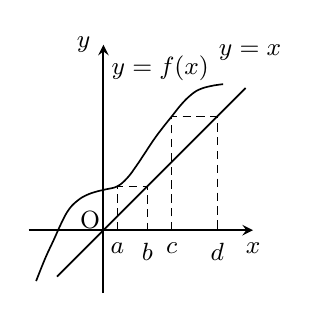
\begin{tikzpicture}[x=0.38cm, y=0.38cm, line width=0.6pt]
  \draw[->, >=stealth, line width=0.7pt] (-2.5,0) -- (5.0,0) node[below=1pt, font=\small] {$x$};
  \draw[->, >=stealth, line width=0.7pt] (0,-2.1) -- (0,6.2) node[left=1pt, font=\small] {$y$};
  \draw[densely dashed, line width=0.4pt] (0.47,0) -- (0.47,1.47) -- (1.47,1.47) -- (1.47,0);
  \draw[densely dashed, line width=0.4pt] (2.28,0) -- (2.28,3.80) -- (3.80,3.80) -- (3.80,0);
  \draw[line width=0.6pt] (-1.55,-1.55) -- (4.75,4.75);
  \draw plot[smooth, tension=0.7] coordinates {(-2.25,-1.7) (-1.95,-0.95) (-1.65,-0.30) (-1.40,0.25) (-1.15,0.70) (-0.85,1.00) (-0.55,1.18) (-0.20,1.30) (0.10,1.37) (0.47,1.47) (0.8,1.75) (1.1,2.15) (1.4,2.60) (1.7,3.05) (2.0,3.45) (2.28,3.80) (2.6,4.20) (2.9,4.50) (3.2,4.70) (3.6,4.82) (4.0,4.88)};
  \node[font=\small] at (-0.45,0.33) {$\pt{O}$};
  \node[below=1pt, font=\small] at (0.47,0) {$a$};
  \node[below=1pt, font=\small] at (1.47,0) {$b$};
  \node[below=1pt, font=\small] at (2.28,0) {$c$};
  \node[below=1pt, font=\small] at (3.80,0) {$d$};
  \node[font=\small] at (1.9,5.4) {$y=f(x)$};
  \node[font=\small] at (4.9,5.95) {$y=x$};
\end{tikzpicture}
}\end{minipage}\par
\dmchoicesauto{\rule[-3ex]{0pt}{8ex}}{$\dfrac{b-a}{b-d}$}{$\dfrac{d-c}{b-d}$}{$\dfrac{b-a}{d-b}$}{$\dfrac{c-b}{d-b}$}{$\dfrac{c-a}{d-b}$}
}\vspace{8mm}
\dmsection{유형 03 평균변화율과 미분계수}
\setcounter{dmproblemcount}{7}\dmpnum{32-08}{% id: 32-08
% book: 쎈B 미적분1 · 03 미분계수와 도함수
% section: 유형 03 평균변화율과 미분계수
% figure: none
% answer: 
% answer_source: 
% variant_level: 0 (원본 전사)
% 이 파일은 build.mjs 가 items.json 에서 만든다. 고칠 때는 items.json 을 고친다.
\smash{\raisebox{1.5mm}{\dmkichul{쎈B 미적분1 32쪽 08번 · 대표 문제}}}
함수 $f(x)=x^2-3x$에서 $x$의 값이 1에서 4까지 변할 때의 평균변화율과 $x=a$에서의 미분계수가 같을 때, 상수 $a$의 값을 구하시오.
}\vspace{8mm}
\setcounter{dmproblemcount}{8}\dmpnum{32-09}{% id: 32-09
% book: 쎈B 미적분1 · 03 미분계수와 도함수
% section: 유형 03 평균변화율과 미분계수
% figure: none
% answer: 
% answer_source: 
% variant_level: 0 (원본 전사)
% 이 파일은 build.mjs 가 items.json 에서 만든다. 고칠 때는 items.json 을 고친다.
\smash{\raisebox{1.5mm}{\dmkichul{쎈B 미적분1 32쪽 09번 · 서술형}}}
함수 $f(x)=x^2+5x+1$에서 $x$의 값이 $a$에서 $b$까지 변할 때의 평균변화율과 $x=-2$에서의 순간변화율이 같을 때, 상수 $a$, $b$에 대하여 $a+b$의 값을 구하시오.
}\vspace{8mm}
\setcounter{dmproblemcount}{9}\dmpnum{32-10}{% id: 32-10
% book: 쎈B 미적분1 · 03 미분계수와 도함수
% section: 유형 03 평균변화율과 미분계수
% figure: none
% answer: 
% answer_source: 
% variant_level: 0 (원본 전사)
% 이 파일은 build.mjs 가 items.json 에서 만든다. 고칠 때는 items.json 을 고친다.
\smash{\raisebox{1.5mm}{\dmkichul{쎈B 미적분1 32쪽 10번}}}
다항함수 $f(x)$에 대하여 $f(0)=2$이고, $x$의 값이 0에서 $t$까지 변할 때의 평균변화율이 $t^2-6$일 때, $x=1$에서의 순간변화율은?
\dmchoicesauto{}{$-7$}{$-6$}{$-5$}{$-4$}{$-3$}
}\vspace{8mm}
\dmsection{유형 04 미분계수를 이용한 극한값의 계산; $\lim\limits_{h\to 0}\frac{f(a+h)-f(a)}{h}$}
\vspace{3mm}\setcounter{dmproblemcount}{10}\dmpnum{32-11}{% id: 32-11
% book: 쎈B 미적분1 · 03 미분계수와 도함수
% section: 유형 04 미분계수를 이용한 극한값의 계산; $\lim\limits_{h\to 0}\frac{f(a+h)-f(a)}{h}$
% figure: none
% answer: 
% answer_source: 
% variant_level: 0 (원본 전사)
% 이 파일은 build.mjs 가 items.json 에서 만든다. 고칠 때는 items.json 을 고친다.
\smash{\raisebox{4.5mm}{\dmkichul{쎈B 미적분1 32쪽 11번 · 대표 문제}}}
다항함수 $f(x)$에 대하여 $f'(1)=-3$일 때,\par\smallskip\dispeq{$\displaystyle\lim_{h\to 0}\dfrac{f(1-h)-f(1+5h)}{h}$}\par\smallskip\noindent 의 값을 구하시오.
}\vspace{8mm}
\vspace{3mm}\setcounter{dmproblemcount}{11}\dmpnum{32-12}{% id: 32-12
% book: 쎈B 미적분1 · 03 미분계수와 도함수
% section: 유형 04 미분계수를 이용한 극한값의 계산; $\lim\limits_{h\to 0}\frac{f(a+h)-f(a)}{h}$
% figure: none
% answer: 
% answer_source: 
% variant_level: 0 (원본 전사)
% 이 파일은 build.mjs 가 items.json 에서 만든다. 고칠 때는 items.json 을 고친다.
\smash{\raisebox{4.5mm}{\dmkichul{쎈B 미적분1 32쪽 12번}}}
다항함수 $f(x)$에 대하여 $\displaystyle\lim_{h\to 0}\dfrac{f(a+4h)-f(a)}{7h}$를 $f'(a)$를 이용하여 나타내면?
\dmchoicesauto{\rule[-3ex]{0pt}{8ex}}{$\dfrac{1}{7}f'(a)$}{$\dfrac{4}{7}f'(a)$}{$\dfrac{7}{4}f'(a)$}{$4f'(a)$}{$7f'(a)$}
}\vspace{8mm}
\vspace{3mm}\setcounter{dmproblemcount}{12}\dmpnum{33-13}{% id: 33-13
% book: 쎈B 미적분1 · 03 미분계수와 도함수
% section: 유형 04 미분계수를 이용한 극한값의 계산; $\lim\limits_{h\to 0}\frac{f(a+h)-f(a)}{h}$
% figure: none
% answer: 
% answer_source: 
% variant_level: 0 (원본 전사)
% 이 파일은 build.mjs 가 items.json 에서 만든다. 고칠 때는 items.json 을 고친다.
\smash{\raisebox{4.5mm}{\dmkichul{쎈B 미적분1 33쪽 13번}}}
다항함수 $f(x)$가 모든 실수 $x$에 대하여 $f(x)=-f(-x)$를 만족시키고 $f(-8)=-4$, $f'(8)=5$일 때, $\displaystyle\lim_{h\to 0}\dfrac{f(8-h)-4}{h}$의 값은?
\dmchoicesauto{}{$-5$}{$-4$}{$-3$}{$-2$}{$-1$}
}\vspace{8mm}
\vspace{3mm}\setcounter{dmproblemcount}{13}\dmpnum{33-14}{% id: 33-14
% book: 쎈B 미적분1 · 03 미분계수와 도함수
% section: 유형 04 미분계수를 이용한 극한값의 계산; $\lim\limits_{h\to 0}\frac{f(a+h)-f(a)}{h}$
% figure: none
% answer: 
% answer_source: 
% variant_level: 0 (원본 전사)
% 이 파일은 build.mjs 가 items.json 에서 만든다. 고칠 때는 items.json 을 고친다.
\smash{\raisebox{4.5mm}{\dmkichul{쎈B 미적분1 33쪽 14번}}}
다항함수 $f(x)$에 대하여 \par\smallskip\dispeq{$\displaystyle\lim_{h\to 0}\dfrac{\sqrt{f(a+h)}-\sqrt{f(a)}}{h}$}\par\smallskip\noindent 를 $f(a)$, $f'(a)$를 이용하여 나타내면? \dmcondfill{$f(a)>0$}{}
\begin{choices32}{\rule[-3ex]{0pt}{8ex}$\dfrac{f'(a)}{\sqrt{f(a)}}$}{\rule[-3ex]{0pt}{8ex}$\dfrac{f'(a)}{\sqrt{2f(a)}}$}{\rule[-3ex]{0pt}{8ex}$\dfrac{f'(a)}{2\sqrt{f(a)}}$}{\rule[-3ex]{0pt}{8ex}$\dfrac{f'(a)}{f(a)}$}{\rule[-3ex]{0pt}{8ex}$\dfrac{f'(a)}{2f(a)}$}\end{choices32}
}\vspace{8mm}
\vspace{3mm}\setcounter{dmproblemcount}{14}\dmpnum{33-15}{% id: 33-15
% book: 쎈B 미적분1 · 03 미분계수와 도함수
% section: 유형 04 미분계수를 이용한 극한값의 계산; $\lim\limits_{h\to 0}\frac{f(a+h)-f(a)}{h}$
% figure: none
% answer: 
% answer_source: 
% variant_level: 0 (원본 전사)
% 이 파일은 build.mjs 가 items.json 에서 만든다. 고칠 때는 items.json 을 고친다.
\smash{\raisebox{4.5mm}{\dmkichul{쎈B 미적분1 33쪽 15번}}}
미분가능한 함수 $f(x)$에 대하여 \par\smallskip\dispeq{$\displaystyle\lim_{h\to 0}\dfrac{f(a+2h)-f(a)}{h}=2$}\par\smallskip\noindent 일 때, $\displaystyle\lim_{h\to 0}\dfrac{f(a-3h)-f(a+h^2)}{h}$의 값을 구하시오.
}\vspace{8mm}
\dmsection{유형 05 미분계수를 이용한 극한값의 계산; $\lim\limits_{x\to a}\frac{f(x)-f(a)}{x-a}$}
\vspace{3mm}\setcounter{dmproblemcount}{15}\dmpnum{33-16}{% id: 33-16
% book: 쎈B 미적분1 · 03 미분계수와 도함수
% section: 유형 05 미분계수를 이용한 극한값의 계산; $\lim\limits_{x\to a}\frac{f(x)-f(a)}{x-a}$
% figure: none
% answer: 
% answer_source: 
% variant_level: 0 (원본 전사)
% 이 파일은 build.mjs 가 items.json 에서 만든다. 고칠 때는 items.json 을 고친다.
\smash{\raisebox{4.5mm}{\dmkichul{쎈B 미적분1 33쪽 16번 · 대표 문제}}}
다항함수 $f(x)$에 대하여 $f(1)=3$, $f'(1)=2$일 때, $\displaystyle\lim_{x\to 1}\dfrac{x^2f(1)-f(x)}{x-1}$의 값을 구하시오.
}\vspace{8mm}
\vspace{3mm}\setcounter{dmproblemcount}{16}\dmpnum{33-17}{% id: 33-17
% book: 쎈B 미적분1 · 03 미분계수와 도함수
% section: 유형 05 미분계수를 이용한 극한값의 계산; $\lim\limits_{x\to a}\frac{f(x)-f(a)}{x-a}$
% figure: none
% answer: 
% answer_source: 
% variant_level: 0 (원본 전사)
% 이 파일은 build.mjs 가 items.json 에서 만든다. 고칠 때는 items.json 을 고친다.
\smash{\raisebox{4.5mm}{\dmkichul{쎈B 미적분1 33쪽 17번}}}
다항함수 $f(x)$에 대하여 $f(2)=0$, $f'(2)=10$일 때, $\displaystyle\lim_{x\to 2}\dfrac{f(x)}{x^2+x-6}$의 값은?
\dmchoicesauto{\rule[-3ex]{0pt}{8ex}}{$\dfrac{1}{2}$}{$1$}{$\dfrac{3}{2}$}{$2$}{$\dfrac{5}{2}$}
}\vspace{8mm}
\vspace{3mm}\setcounter{dmproblemcount}{17}\dmpnum{33-18}{% id: 33-18
% book: 쎈B 미적분1 · 03 미분계수와 도함수
% section: 유형 05 미분계수를 이용한 극한값의 계산; $\lim\limits_{x\to a}\frac{f(x)-f(a)}{x-a}$
% figure: none
% answer: 
% answer_source: 
% variant_level: 0 (원본 전사)
% 이 파일은 build.mjs 가 items.json 에서 만든다. 고칠 때는 items.json 을 고친다.
\smash{\raisebox{4.5mm}{\dmkichul{쎈B 미적분1 33쪽 18번}}}
다항함수 $f(x)$에 대하여 $f(3)=9$, $f'(3)=6$일 때, $\displaystyle\lim_{x\to 3}\dfrac{\sqrt{f(x)}-3}{\sqrt{x}-\sqrt{3}}$의 값을 구하시오.
}\vspace{8mm}
\vspace{3mm}\setcounter{dmproblemcount}{18}\dmpnum{33-19}{% id: 33-19
% book: 쎈B 미적분1 · 03 미분계수와 도함수
% section: 유형 05 미분계수를 이용한 극한값의 계산; $\lim\limits_{x\to a}\frac{f(x)-f(a)}{x-a}$
% figure: none
% answer: 
% answer_source: 
% variant_level: 0 (원본 전사)
% 이 파일은 build.mjs 가 items.json 에서 만든다. 고칠 때는 items.json 을 고친다.
\smash{\raisebox{4.5mm}{\dmkichul{쎈B 미적분1 33쪽 19번 · 서술형}}}
다항함수 $f(x)$에 대하여 $\displaystyle\lim_{x\to-1}\dfrac{f(x+5)-4}{x^2-1}=7$일 때, $f(4)+f'(4)$의 값을 구하시오.
}\vspace{8mm}
\setcounter{dmproblemcount}{19}\dmpnum{34-20}{% id: 34-20
% book: 쎈B 미적분1 · 03 미분계수와 도함수
% section: 유형 05 미분계수를 이용한 극한값의 계산; $\lim\limits_{x\to a}\frac{f(x)-f(a)}{x-a}$
% figure: none
% answer: 
% answer_source: 
% variant_level: 0 (원본 전사)
% 이 파일은 build.mjs 가 items.json 에서 만든다. 고칠 때는 items.json 을 고친다.
\smash{\raisebox{1.5mm}{\dmkichul{쎈B 미적분1 34쪽 20번}}}
두 다항함수 $f(x)$, $g(x)$가 다음 조건을 모두 만족시킬 때, $f'(2)g'(2)$의 값을 구하시오. \exprbox{\begin{minipage}{0.96\linewidth}\raggedright ㈎ $\displaystyle\lim_{x\to 2}\dfrac{f(x)-3g(x)}{x-2}=4$\par\smallskip ㈏ $\displaystyle\lim_{x\to 2}\dfrac{f(x)+3g(x)-2f(2)}{x-2}=6$\end{minipage}}
}\vspace{8mm}
\dmsection{유형 06 항등식이 주어질 때 미분계수 구하기}
\setcounter{dmproblemcount}{20}\dmpnum{34-21}{% id: 34-21
% book: 쎈B 미적분1 · 03 미분계수와 도함수
% section: 유형 06 항등식이 주어질 때 미분계수 구하기
% figure: none
% answer: 
% answer_source: 
% variant_level: 0 (원본 전사)
% 이 파일은 build.mjs 가 items.json 에서 만든다. 고칠 때는 items.json 을 고친다.
\smash{\raisebox{1.5mm}{\dmkichul{쎈B 미적분1 34쪽 21번 · 대표 문제}}}
미분가능한 함수 $f(x)$가 모든 실수 $x$, $y$에 대하여 \par\smallskip\dispeq{$f(x+y)=f(x)+f(y)$}\par\smallskip\noindent 를 만족시키고 $f'(0)=-1$일 때, $f'(2)$의 값은?
\dmchoicesauto{}{$-5$}{$-4$}{$-3$}{$-2$}{$-1$}
}\vspace{8mm}
\setcounter{dmproblemcount}{21}\dmpnum{34-22}{% id: 34-22
% book: 쎈B 미적분1 · 03 미분계수와 도함수
% section: 유형 06 항등식이 주어질 때 미분계수 구하기
% figure: none
% answer: 
% answer_source: 
% variant_level: 0 (원본 전사)
% 이 파일은 build.mjs 가 items.json 에서 만든다. 고칠 때는 items.json 을 고친다.
\smash{\raisebox{1.5mm}{\dmkichul{쎈B 미적분1 34쪽 22번 · 서술형}}}
미분가능한 함수 $f(x)$가 모든 실수 $x$, $y$에 대하여 \par\smallskip\dispeq{$f(x+y)=f(x)+f(y)+xy$}\par\smallskip\noindent 를 만족시키고 $f'(1)=4$일 때, $f'(3)$의 값을 구하시오.
}\vspace{8mm}
\setcounter{dmproblemcount}{22}\dmpnum{34-23}{% id: 34-23
% book: 쎈B 미적분1 · 03 미분계수와 도함수
% section: 유형 06 항등식이 주어질 때 미분계수 구하기
% figure: none
% answer: 
% answer_source: 
% variant_level: 0 (원본 전사)
% 이 파일은 build.mjs 가 items.json 에서 만든다. 고칠 때는 items.json 을 고친다.
\smash{\raisebox{1.5mm}{\dmkichul{쎈B 미적분1 34쪽 23번}}}
미분가능한 함수 $f(x)$가 모든 실수 $x$, $y$에 대하여 \par\smallskip\dispeq{$f(x+y)=f(x)+f(y)+3xy-1$}\par\smallskip\noindent 을 만족시키고 $f'(2)=8$, $f'(2a)=20$일 때, 상수 $a$의 값은?
\dmchoicesauto{}{$2$}{$3$}{$4$}{$5$}{$6$}
}\vspace{8mm}
\vspace{3mm}\setcounter{dmproblemcount}{23}\dmpnum{34-24}{% id: 34-24
% book: 쎈B 미적분1 · 03 미분계수와 도함수
% section: 유형 06 항등식이 주어질 때 미분계수 구하기
% figure: none
% answer: 
% answer_source: 
% variant_level: 0 (원본 전사)
% 이 파일은 build.mjs 가 items.json 에서 만든다. 고칠 때는 items.json 을 고친다.
\smash{\raisebox{4.5mm}{\dmkichul{쎈B 미적분1 34쪽 24번}}}
미분가능한 함수 $f(x)$가 모든 실수 $x$, $y$에 대하여 $f(x+y)=4f(x)f(y)$, $f(x)>0$을 만족시킨다. $f'(0)=-3$일 때, $\dfrac{f'(10)}{f(10)}$의 값을 구하시오.
}\vspace{8mm}
\dmsection{유형 07 미분계수의 기하적 의미}
\vspace{3mm}\setcounter{dmproblemcount}{24}\dmpnum{34-25}{% id: 34-25
% book: 쎈B 미적분1 · 03 미분계수와 도함수
% section: 유형 07 미분계수의 기하적 의미
% figure: tikz:fig-34-25
% answer: 
% answer_source: 
% variant_level: 0 (원본 전사)
% 이 파일은 build.mjs 가 items.json 에서 만든다. 고칠 때는 items.json 을 고친다.
\smash{\raisebox{4.5mm}{\dmkichul{쎈B 미적분1 34쪽 25번 · 대표 문제}}}
\noindent\begin{minipage}[t]{0.58\linewidth}\vspace{0pt}\raggedright 함수 $y=f(x)$의 그래프와 이 그래프 위의 $x=1$인 점에서의 접선이 오른쪽 그림과 같을 때, $\displaystyle\lim_{h\to 0}\dfrac{f(1+3h)-f(1)}{4h}$의 값은?\end{minipage}\hfill\begin{minipage}[t]{0.4\linewidth}\vspace{0pt}\centering \resizebox{\ifdim\width>\linewidth\linewidth\else\width\fi}{!}{% 34-25(34쪽) — 함수 $y=f(x)$ 의 그래프와 그 그래프 위의 $x=1$ 인 점에서의 접선. 스캔 화질이 낮아 TikZ 로 다시 그림.
% 원문에 있는 것만 옮긴다: 곡선 · 접선 · 접점으로 가는 안내 점선 둘 · 라벨 y=f(x), 5, 3, O, 1, x, y. 원문에 없는 눈금은 만들지 않는다.
\begin{tikzpicture}[x=0.30cm, y=0.29cm, line width=0.55pt]
  \draw[->, >=stealth, line width=0.7pt] (-7.1,0) -- (3.6,0) node[below=2pt, font=\small] {$x$};
  \draw[->, >=stealth, line width=0.7pt] (0,-2.2) -- (0,8.9) node[left=2pt, font=\small] {$y$};
  \draw[densely dashed, line width=0.4pt] (0,3) -- (1,3);
  \draw[densely dotted, line width=0.4pt] (1,3) -- (1,0);
  \draw[line width=0.6pt] plot[smooth, tension=0.7] coordinates {
    (-5.95,7.32) (-5.50,6.34) (-5.00,5.22) (-4.60,4.15) (-4.10,3.27) (-3.70,2.62)
    (-3.20,2.23) (-2.80,2.08) (-2.60,2.05) (-2.40,2.08) (-2.00,2.22) (-1.60,2.55)
    (-1.20,3.05) (-0.80,3.68) (-0.40,4.18) (-0.20,4.27) (0.00,4.30) (0.20,4.23)
    (0.40,4.03) (0.60,3.75) (0.80,3.39) (1.00,3.00) (1.20,2.55) (1.40,2.01)
    (1.60,1.37) (1.80,0.63) (2.00,-0.20) (2.20,-1.13) (2.40,-2.15) };
  \draw[line width=0.5pt] (-1.85,8.70) -- (3.40,-1.80);
  \node[anchor=east, inner sep=1pt, font=\small] at (-3.0,8.3) {$y=f(x)$};
  \node[above right=-3pt and 1pt, font=\small] at (0,5) {$5$};
  \node[left=2pt, font=\small] at (0,3) {$3$};
  \node[below left=-1pt and -2pt, font=\small] at (0,0) {$\pt{O}$};
  \node[below=1pt, font=\small] at (1,0) {$1$};
\end{tikzpicture}
}\end{minipage}\par
\dmchoicesauto{\rule[-3ex]{0pt}{8ex}}{$-\dfrac{7}{2}$}{$-3$}{$-\dfrac{5}{2}$}{$-2$}{$-\dfrac{3}{2}$}
}\vspace{8mm}
\setcounter{dmproblemcount}{25}\dmpnum{35-26}{% id: 35-26
% book: 쎈B 미적분1 · 03 미분계수와 도함수
% section: 유형 07 미분계수의 기하적 의미
% figure: tikz:fig-35-26
% answer: 
% answer_source: 
% variant_level: 0 (원본 전사)
% 이 파일은 build.mjs 가 items.json 에서 만든다. 고칠 때는 items.json 을 고친다.
\smash{\raisebox{1.5mm}{\dmkichul{쎈B 미적분1 35쪽 26번}}}
\noindent\begin{minipage}[t]{0.58\linewidth}\vspace{0pt}\raggedright 모든 실수 $x$에서 미분가능한 함수 $y=f(x)$의 그래프가 오른쪽 그림과 같을 때, 네 수 $f'(a)$, $f'(b)$, $f'(c)$, $f'(d)$의 대소를 비교하시오.\end{minipage}\hfill\begin{minipage}[t]{0.4\linewidth}\vspace{0pt}\centering \resizebox{\ifdim\width>\linewidth\linewidth\else\width\fi}{!}{% 35-26(35쪽) — 모든 실수에서 미분가능한 함수 y=f(x) 의 그래프(봉우리 셋). 스캔 화질이 낮아 TikZ 로 다시 그림.
% 원문에 있는 것만 옮긴다: 곡선 · a·b·c·d 에서 곡선까지 올라가는 안내 점선 넷 · 라벨 y=f(x), O, a, b, c, d, x, y. 눈금값은 원문에 없다.
\begin{tikzpicture}[x=0.95cm, y=0.95cm, line width=0.6pt]
  \draw[->, >=stealth, line width=0.7pt] (-1.55,0) -- (4.70,0) node[below=1pt, font=\small] {$x$};
  \draw[->, >=stealth, line width=0.7pt] (0,-1.65) -- (0,2.15) node[left=1pt, font=\small] {$y$};
  \draw[densely dotted, line width=0.4pt] (-0.485,0) -- (-0.485,0.50);
  \draw[densely dotted, line width=0.4pt] (1.975,0) -- (1.975,1.44);
  \draw[densely dotted, line width=0.4pt] (3.415,0) -- (3.415,1.00);
  \draw[densely dotted, line width=0.4pt] (3.890,0) -- (3.890,1.00);
  \draw plot[smooth, tension=0.6] coordinates {
    (-1.335,-1.125) (-1.085,-0.700) (-0.835,-0.250) (-0.635,0.150) (-0.485,0.500)
    (-0.335,0.825) (-0.185,1.100) (0.015,1.350) (0.165,1.400) (0.365,1.350)
    (0.565,1.200) (0.765,0.975) (0.965,0.650) (1.165,0.300) (1.315,0.075)
    (1.465,0.025) (1.615,0.100) (1.765,0.450) (1.890,1.000) (2.015,1.455)
    (2.115,1.300) (2.215,0.850) (2.340,0.050) (2.465,-0.600) (2.615,-1.200)
    (2.765,-1.410) (2.915,-1.250) (3.065,-0.750) (3.190,-0.025) (3.315,0.600)
    (3.415,1.000) (3.540,1.500) (3.630,1.710) (3.740,1.600) (3.890,1.000)
    (4.015,0.400) (4.115,-0.025) (4.215,-0.650) (4.315,-1.200) };
  \node[below right=-1pt and -1pt, font=\small] at (0,0) {$\pt{O}$};
  \node[below=1pt, font=\small] at (-0.485,0) {$a$};
  \node[below=1pt, font=\small] at (1.975,0) {$b$};
  \node[below=1pt, font=\small] at (3.415,0) {$c$};
  \node[below=1pt, font=\small] at (3.890,0) {$d$};
  \node[anchor=south, font=\small] at (3.30,1.95) {$y=f(x)$};
\end{tikzpicture}
}\end{minipage}\par
}\vspace{8mm}
\vspace{3mm}\setcounter{dmproblemcount}{26}\dmpnum{35-27}{% id: 35-27
% book: 쎈B 미적분1 · 03 미분계수와 도함수
% section: 유형 07 미분계수의 기하적 의미
% figure: none
% answer: 
% answer_source: 
% variant_level: 0 (원본 전사)
% 이 파일은 build.mjs 가 items.json 에서 만든다. 고칠 때는 items.json 을 고친다.
\smash{\raisebox{4.5mm}{\dmkichul{쎈B 미적분1 35쪽 27번}}}
곡선 $y=f(x)$ 위의 점 $(2{,}\mkern3mu\mathopen{}6)$에서의 접선의 기울기가 4일 때, $\displaystyle\lim_{x\to 2}\dfrac{2f(x)-xf(2)}{x-2}$의 값을 구하시오.
}\vspace{8mm}
\vspace{3mm}\setcounter{dmproblemcount}{27}\dmpnum{35-28}{% id: 35-28
% book: 쎈B 미적분1 · 03 미분계수와 도함수
% section: 유형 07 미분계수의 기하적 의미
% figure: tikz:fig-35-28
% answer: 
% answer_source: 
% variant_level: 0 (원본 전사)
% 이 파일은 build.mjs 가 items.json 에서 만든다. 고칠 때는 items.json 을 고친다.
\smash{\raisebox{4.5mm}{\dmkichul{쎈B 미적분1 35쪽 28번}}}
\noindent\begin{minipage}[t]{0.58\linewidth}\vspace{0pt}\raggedright 함수 $y=f(x)$의 그래프는 오른쪽 그림과 같다. $0<a<b$일 때, 옳은 것만을 보기에서 있는 대로 고른 것은? \end{minipage}\hfill\begin{minipage}[t]{0.4\linewidth}\vspace{0pt}\centering \resizebox{\ifdim\width>\linewidth\linewidth\else\width\fi}{!}{% 35-28(35쪽) — 증가하고 아래로 볼록한 함수 y=f(x) 의 그래프와 f(a) · f((a+b)/2) · f(b) 를 잇는 안내 점선.
% 스캔 화질이 낮아 TikZ 로 다시 그림. 원문에 있는 것만 옮긴다: 곡선 · 점선 · 라벨 y=f(x), f(a), f((a+b)/2), f(b), O, a, (a+b)/2, b, x, y.
\begin{tikzpicture}[x=0.95cm, y=0.95cm, line width=0.6pt]
  \draw[->, >=stealth, line width=0.7pt] (-0.75,0) -- (4.35,0) node[below=1pt, font=\small] {$x$};
  \draw[->, >=stealth, line width=0.7pt] (0,-0.55) -- (0,3.55) node[left=1pt, font=\small] {$y$};
  \draw[densely dashed, line width=0.4pt] (0,0.705) -- (1.50,0.705) -- (1.50,0);
  \draw[densely dashed, line width=0.4pt] (0,1.397) -- (2.60,1.397) -- (2.60,0);
  \draw[densely dashed, line width=0.4pt] (0,2.769) -- (3.70,2.769) -- (3.70,0);
  \draw[line width=0.6pt, domain=-0.60:4.05, samples=120, smooth] plot (\x, {0.28*exp(0.62*\x)});
  \node[anchor=south, font=\small] at (2.25,3.15) {$y=f(x)$};
  \node[left=2pt, font=\small] at (0,2.769) {$f(b)$};
  \node[left=2pt, font=\small] at (0,1.397) {$f\!\left(\dfrac{a+b}{2}\right)$};
  \node[left=2pt, font=\small] at (0,0.705) {$f(a)$};
  \node[below left=-1pt and -2pt, font=\small] at (0,0) {$\pt{O}$};
  \node[below=1pt, font=\small] at (1.50,0) {$a$};
  \node[below=1pt, font=\small] at (2.60,0) {$\dfrac{a+b}{2}$};
  \node[below=1pt, font=\small] at (3.70,0) {$b$};
\end{tikzpicture}
}\end{minipage}\par
\noindent \bogi{ㄱ. $f'(a)<f'(b)$\\ ㄴ. $f\!\left(\dfrac{a+b}{2}\right)<\dfrac{f(a)+f(b)}{2}$\\ ㄷ. $f'(a)>\dfrac{f(b)-f(a)}{b-a}$}
\dmchoicesauto{}{ㄱ}{ㄱ, ㄴ}{ㄱ, ㄷ}{ㄴ, ㄷ}{ㄱ, ㄴ, ㄷ}
}\vspace{8mm}
\setcounter{dmproblemcount}{28}\dmpnum{35-29}{% id: 35-29
% book: 쎈B 미적분1 · 03 미분계수와 도함수
% section: 유형 07 미분계수의 기하적 의미
% figure: tikz:fig-35-29
% answer: 
% answer_source: 
% variant_level: 0 (원본 전사)
% 이 파일은 build.mjs 가 items.json 에서 만든다. 고칠 때는 items.json 을 고친다.
\smash{\raisebox{1.5mm}{\dmkichul{쎈B 미적분1 35쪽 29번}}}
\noindent\begin{minipage}[t]{0.58\linewidth}\vspace{0pt}\raggedright 오른쪽 그림은 함수 $y=f(x)$의 그래프와 직선 $y=2x$를 나타낸 것이다. $0<a<b$일 때, 다음 중 옳지 않은 것은?\end{minipage}\hfill\begin{minipage}[t]{0.4\linewidth}\vspace{0pt}\centering \resizebox{\ifdim\width>\linewidth\linewidth\else\width\fi}{!}{% 35-29(35쪽) — 원점을 지나 증가하며 위로 볼록한 함수 y=f(x) 의 그래프와 직선 y=2x. 스캔 화질이 낮아 TikZ 로 다시 그림.
% 원문에 있는 것만 옮긴다: 곡선 · 직선 · a·b 에서 곡선까지 올라가는 안내 점선 둘 · 라벨 y=2x, y=f(x), O, a, b, x, y.
\begin{tikzpicture}[x=0.95cm, y=0.95cm, line width=0.6pt]
  \draw[->, >=stealth, line width=0.7pt] (-0.95,0) -- (4.45,0) node[below=1pt, font=\small] {$x$};
  \draw[->, >=stealth, line width=0.7pt] (0,-1.25) -- (0,3.05) node[left=1pt, font=\small] {$y$};
  \draw[densely dotted, line width=0.4pt] (1.90,0) -- (1.90,1.68);
  \draw[densely dotted, line width=0.4pt] (2.95,0) -- (2.95,2.11);
  \draw[line width=0.6pt] (-0.55,-1.10) -- (1.35,2.70);
  \draw[line width=0.6pt, domain=0:4.20, samples=120, smooth] plot (\x, {2.75*(1-exp(-0.50*\x))});
  \node[anchor=south west, font=\small] at (1.05,2.55) {$y=2x$};
  \node[anchor=south, font=\small] at (3.35,2.35) {$y=f(x)$};
  \node[below right=-1pt and -1pt, font=\small] at (0,0) {$\pt{O}$};
  \node[below=1pt, font=\small] at (1.90,0) {$a$};
  \node[below=1pt, font=\small] at (2.95,0) {$b$};
\end{tikzpicture}
}\end{minipage}\par
\begin{choicesv}{$f(b)-f(a)<2(b-a)$}{$bf(a)-af(b)>0$}{$f'(a)>f'(b)$}{$f(a)<af'(a)$}{$f'(a+b)<f'(2\sqrt{ab})$}\end{choicesv}
}\vspace{8mm}
\dmsection{유형 08 미분가능성과 연속성}
\setcounter{dmproblemcount}{29}\dmpnum{35-30}{% id: 35-30
% book: 쎈B 미적분1 · 03 미분계수와 도함수
% section: 유형 08 미분가능성과 연속성
% figure: none
% answer: 
% answer_source: 
% variant_level: 0 (원본 전사)
% 이 파일은 build.mjs 가 items.json 에서 만든다. 고칠 때는 items.json 을 고친다.
\smash{\raisebox{1.5mm}{\dmkichul{쎈B 미적분1 35쪽 30번 · 대표 문제}}}
다음 중 $x=0$에서 연속이지만 미분가능하지 않은 함수는?
\begin{choicesii}{\rule[-3ex]{0pt}{8ex}$f(x)=x$}{\rule[-3ex]{0pt}{8ex}$f(x)=\sqrt{x^2}$}{\rule[-3ex]{0pt}{8ex}$f(x)=|x|^2$}{\rule[-3ex]{0pt}{8ex}$f(x)=\dfrac{x^2}{|x|}$}{\rule[-3ex]{0pt}{8ex}$f(x)=\begin{cases} x^2 & (x\ge 0) \\ -x^2 & (x<0) \end{cases}$}\end{choicesii}
}\vspace{8mm}
\setcounter{dmproblemcount}{30}\dmpnum{36-31}{% id: 36-31
% book: 쎈B 미적분1 · 03 미분계수와 도함수
% section: 유형 08 미분가능성과 연속성
% figure: none
% answer: 
% answer_source: 
% variant_level: 0 (원본 전사)
% 이 파일은 build.mjs 가 items.json 에서 만든다. 고칠 때는 items.json 을 고친다.
\smash{\raisebox{1.5mm}{\dmkichul{쎈B 미적분1 36쪽 31번}}}
다음 함수 $y=f(x)$의 그래프 중 $x=a$에서 미분가능한 것은?
\begin{choicesii}{% 36-31 ①(36쪽) — 보기 그래프: 증가하는 직선인데 x=a 에서 빈 점(끊김). 보기 자체가 그림이라 TikZ 로 다시 그림.
% 라벨은 원문 그대로 y=f(x), O, a, x, y 만(보기 다섯 개를 나란히 두려고 작은 글자로).
\begin{tikzpicture}[scale=0.62, line width=0.5pt, baseline=(current bounding box.center)]
  \path (-2.3,-1.6) rectangle (3.1,2.7);
  \draw[->, >=stealth, line width=0.7pt] (-2.1,0) -- (2.85,0) node[below=1pt, font=\scriptsize] {$x$};
  \draw[->, >=stealth, line width=0.7pt] (0,-1.15) -- (0,2.35) node[left=1pt, font=\scriptsize] {$y$};
  \draw[line width=0.6pt] (-2.0,-0.385) -- (2.7,2.2);
  \draw[densely dotted, line width=0.4pt] (0.9,0) -- (0.9,1.215);
  \draw[fill=white] (0.9,1.215) circle (1.8pt);
  \node[anchor=south, font=\scriptsize] at (1.35,2.05) {$y=f(x)$};
  \node[below left=-2pt and -2pt, font=\scriptsize] at (0,0) {$\pt{O}$};
  \node[below=1pt, font=\scriptsize] at (0.9,0) {$a$};
\end{tikzpicture}
}{% 36-31 ②(36쪽) — 보기 그래프: x<a 는 증가하는 직선(x=a 에서 채운 점), x>a 는 가로 반직선(x=a 에서 빈 점)으로 뛰어 끊긴 그래프.
% 보기 자체가 그림이라 TikZ 로 다시 그림. 라벨은 원문 그대로 y=f(x), O, a, x, y 만.
\begin{tikzpicture}[scale=0.62, line width=0.5pt, baseline=(current bounding box.center)]
  \path (-2.3,-1.6) rectangle (3.1,2.7);
  \draw[->, >=stealth, line width=0.7pt] (-2.1,0) -- (2.85,0) node[below=1pt, font=\scriptsize] {$x$};
  \draw[->, >=stealth, line width=0.7pt] (0,-1.15) -- (0,2.35) node[left=1pt, font=\scriptsize] {$y$};
  \draw[line width=0.6pt] (-2.0,-1.145) -- (0.75,0);
  \draw[line width=0.6pt] (0.75,1.15) -- (2.7,1.15);
  \draw[densely dotted, line width=0.4pt] (0.75,0) -- (0.75,1.15);
  \fill (0.75,0) circle (1.8pt);
  \draw[fill=white] (0.75,1.15) circle (1.8pt);
  \node[anchor=south, font=\scriptsize] at (1.75,1.30) {$y=f(x)$};
  \node[below left=-2pt and -2pt, font=\scriptsize] at (0,0) {$\pt{O}$};
  \node[below=1pt, font=\scriptsize] at (0.75,0) {$a$};
\end{tikzpicture}
}{% 36-31 ③(36쪽) — 보기 그래프: x=a 에서 꺾인 V 모양(절댓값 꼴). 보기 자체가 그림이라 TikZ 로 다시 그림.
% 라벨은 원문 그대로 y=f(x), O, a, x, y 만.
\begin{tikzpicture}[scale=0.62, line width=0.5pt, baseline=(current bounding box.center)]
  \path (-2.3,-1.6) rectangle (3.1,2.7);
  \draw[->, >=stealth, line width=0.7pt] (-2.1,0) -- (2.85,0) node[below=1pt, font=\scriptsize] {$x$};
  \draw[->, >=stealth, line width=0.7pt] (0,-1.15) -- (0,2.35) node[left=1pt, font=\scriptsize] {$y$};
  \draw[line width=0.6pt] (-1.35,2.30) -- (0.55,0.60) -- (2.45,2.30);
  \draw[densely dotted, line width=0.4pt] (0.55,0) -- (0.55,0.60);
  \node[anchor=west, font=\scriptsize] at (1.15,0.45) {$y=f(x)$};
  \node[below left=-2pt and -2pt, font=\scriptsize] at (0,0) {$\pt{O}$};
  \node[below=1pt, font=\scriptsize] at (0.55,0) {$a$};
\end{tikzpicture}
}{% 36-31 ④(36쪽) — 보기 그래프: x=a 에서 x축에 닿으며 왼쪽은 완만하게, 오른쪽은 가파르게 올라가 뾰족한 점이 생기는 그래프.
% 보기 자체가 그림이라 TikZ 로 다시 그림. 라벨은 원문 그대로 y=f(x), O, a, x, y 만.
\begin{tikzpicture}[scale=0.62, line width=0.5pt, baseline=(current bounding box.center)]
  \path (-2.3,-1.6) rectangle (3.1,2.7);
  \draw[->, >=stealth, line width=0.7pt] (-2.1,0) -- (2.85,0) node[below=1pt, font=\scriptsize] {$x$};
  \draw[->, >=stealth, line width=0.7pt] (0,-1.15) -- (0,2.35) node[left=1pt, font=\scriptsize] {$y$};
  \draw[line width=0.6pt, domain=-1.35:0.6, samples=100, smooth] plot (\x, {0.55*(0.6-\x)*(0.6-\x)});
  \draw[line width=0.6pt, domain=0.6:2.7, samples=100, smooth] plot (\x, {1.20*sqrt(\x-0.6)});
  \node[anchor=south east, font=\scriptsize] at (2.80,1.90) {$y=f(x)$};
  \node[below left=-2pt and -2pt, font=\scriptsize] at (0,0) {$\pt{O}$};
  \node[below=1pt, font=\scriptsize] at (0.6,0) {$a$};
\end{tikzpicture}
}{% 36-31 ⑤(36쪽) — 보기 그래프: 꼭짓점이 x=a 인 위로 볼록한 포물선. 보기 자체가 그림이라 TikZ 로 다시 그림.
% 라벨은 원문 그대로 y=f(x), O, a, x, y 만.
\begin{tikzpicture}[scale=0.62, line width=0.5pt, baseline=(current bounding box.center)]
  \path (-2.3,-1.6) rectangle (3.1,2.7);
  \draw[->, >=stealth, line width=0.7pt] (-2.1,0) -- (2.85,0) node[below=1pt, font=\scriptsize] {$x$};
  \draw[->, >=stealth, line width=0.7pt] (0,-1.15) -- (0,2.35) node[left=1pt, font=\scriptsize] {$y$};
  \draw[line width=0.6pt, domain=-1.1:2.6, samples=120, smooth] plot (\x, {1.30-0.72*(\x-0.75)*(\x-0.75)});
  \draw[densely dotted, line width=0.4pt] (0.75,0) -- (0.75,1.30);
  \node[anchor=south, font=\scriptsize] at (1.20,1.50) {$y=f(x)$};
  \node[below left=-2pt and -2pt, font=\scriptsize] at (0,0) {$\pt{O}$};
  \node[below=1pt, font=\scriptsize] at (0.75,0) {$a$};
\end{tikzpicture}
}\end{choicesii}
}\vspace{8mm}
\setcounter{dmproblemcount}{31}\dmpnum{36-32}{% id: 36-32
% book: 쎈B 미적분1 · 03 미분계수와 도함수
% section: 유형 08 미분가능성과 연속성
% figure: none
% answer: 
% answer_source: 
% variant_level: 0 (원본 전사)
% 이 파일은 build.mjs 가 items.json 에서 만든다. 고칠 때는 items.json 을 고친다.
\smash{\raisebox{1.5mm}{\dmkichul{쎈B 미적분1 36쪽 32번}}}
$x=1$에서 연속이지만 미분가능하지 않은 함수인 것만을 보기에서 있는 대로 고른 것은? \bogi{ㄱ. $f(x)=|x(x-1)|$\\ ㄴ. $g(x)=(x-1)|x-1|$\\ ㄷ. $k(x)=x-1+|x-1|$}
\dmchoicesauto{}{ㄱ}{ㄴ}{ㄷ}{ㄱ, ㄴ}{ㄱ, ㄷ}
}\vspace{8mm}
\setcounter{dmproblemcount}{32}\dmpnum{36-33}{% id: 36-33
% book: 쎈B 미적분1 · 03 미분계수와 도함수
% section: 유형 08 미분가능성과 연속성
% figure: tikz:fig-36-33
% answer: 
% answer_source: 
% variant_level: 0 (원본 전사)
% 이 파일은 build.mjs 가 items.json 에서 만든다. 고칠 때는 items.json 을 고친다.
\smash{\raisebox{1.5mm}{\dmkichul{쎈B 미적분1 36쪽 33번}}}
\noindent\begin{minipage}[t]{0.58\linewidth}\vspace{0pt}\raggedright 구간 $(-3{,}\mkern3mu\mathopen{}3)$에서 함수 $y=f(x)$의 그래프가 오른쪽 그림과 같을 때, 다음 중 옳지 않은 것은?\end{minipage}\hfill\begin{minipage}[t]{0.4\linewidth}\vspace{0pt}\centering \resizebox{\ifdim\width>\linewidth\linewidth\else\width\fi}{!}{% 36-33(36쪽) — 구간 (-3, 3) 에서 정의된 함수 y=f(x) 의 그래프(x=-1 에 빈 점·채운 점, x=1 에 뾰족한 점, x=2 에서 끊김).
% 스캔 화질이 낮아 TikZ 로 다시 그림. 원문에 있는 것만 옮긴다: 곡선 · 빈 점·채운 점 · 안내 점선 · 라벨 y=f(x), -3, -2, -1, O, 1, 2, 3, x, y.
\begin{tikzpicture}[x=0.68cm, y=0.68cm, line width=0.6pt]
  \draw[->, >=stealth, line width=0.7pt] (-3.70,0) -- (3.90,0) node[below=1pt, font=\small] {$x$};
  \draw[->, >=stealth, line width=0.7pt] (0,-0.50) -- (0,2.75) node[left=1pt, font=\small] {$y$};
  \draw[densely dotted, line width=0.4pt] (-3,0) -- (-3,1.30);
  \draw[densely dotted, line width=0.4pt] (-2,0) -- (-2,1.90);
  \draw[densely dotted, line width=0.4pt] (-1,0) -- (-1,1.70);
  \draw[densely dotted, line width=0.4pt] (2,0) -- (2,1.10);
  \draw[densely dotted, line width=0.4pt] (3,0) -- (3,1.95);
  \draw[line width=0.6pt] plot[smooth, tension=0.6] coordinates {
    (-3,1.30) (-2.60,1.60) (-2.30,1.78) (-2.00,1.90) (-1.75,1.95) (-1.50,1.92)
    (-1.25,1.83) (-1.00,1.70) (-0.60,1.50) (-0.20,1.26) (0.20,1.00) (0.55,0.70)
    (0.80,0.42) (0.92,0.20) (1,0) };
  \draw[line width=0.6pt] plot[smooth, tension=0.6] coordinates {
    (1,0) (1.20,0.30) (1.45,0.50) (1.70,0.59) (2,0.62) };
  \draw[line width=0.6pt] plot[smooth, tension=0.6] coordinates {
    (2,1.10) (2.30,1.48) (2.60,1.72) (3,1.95) };
  \draw[fill=white] (-3,1.30) circle (2.2pt);
  \draw[fill=white] (-1,1.70) circle (2.2pt);
  \draw[fill=white] (2,1.10) circle (2.2pt);
  \draw[fill=white] (3,1.95) circle (2.2pt);
  \fill (-1,0.85) circle (2.2pt);
  \fill (2,0.62) circle (2.2pt);
  \node[below=1pt, font=\small] at (-3,0) {$-3$};
  \node[below=1pt, font=\small] at (-2,0) {$-2$};
  \node[below=1pt, font=\small] at (-1,0) {$-1$};
  \node[below right=-1pt and -1pt, font=\small] at (0,0) {$\pt{O}$};
  \node[below=1pt, font=\small] at (1,0) {$1$};
  \node[below=1pt, font=\small] at (2,0) {$2$};
  \node[below=1pt, font=\small] at (3,0) {$3$};
  \node[anchor=south east, font=\small] at (3.85,2.10) {$y=f(x)$};
\end{tikzpicture}
}\end{minipage}\par
\par\medskip\par\noindent\hangindent=1.4em\hangafter=1 {\small ①}\ $f'(-2)>0$이다.\par\noindent\hangindent=1.4em\hangafter=1 {\small ②}\ $\displaystyle\lim_{x\to-1} f(x)$의 값이 존재한다.\par\noindent\hangindent=1.4em\hangafter=1 {\small ③}\ $f'(x)=0$인 점은 1개이다.\par\noindent\hangindent=1.4em\hangafter=1 {\small ④}\ 함수 $f(x)$는 $x=-1$, $x=2$에서 불연속이다.\par\noindent\hangindent=1.4em\hangafter=1 {\small ⑤}\ 함수 $f(x)$가 미분가능하지 않은 점은 2개이다.\par\medskip
}\vspace{8mm}
\dmsection{유형 09 구간에 따라 다르게 정의된 함수의 미분가능성}
\vspace{5mm}\setcounter{dmproblemcount}{33}\dmpnum{36-34}{% id: 36-34
% book: 쎈B 미적분1 · 03 미분계수와 도함수
% section: 유형 09 구간에 따라 다르게 정의된 함수의 미분가능성
% figure: none
% answer: 
% answer_source: 
% variant_level: 0 (원본 전사)
% 이 파일은 build.mjs 가 items.json 에서 만든다. 고칠 때는 items.json 을 고친다.
\smash{\raisebox{6.5mm}{\dmkichul{쎈B 미적분1 36쪽 34번 · 대표 문제}}}
함수 $f(x)=\begin{cases} ax^2-1 & (x\ge 2) \\ 8x+b & (x<2) \end{cases}$가 $x=2$에서 미분가능할 때, 상수 $a$, $b$에 대하여 $a+b$의 값을 구하시오.
}\vspace{8mm}
\vspace{5mm}\setcounter{dmproblemcount}{34}\dmpnum{36-35}{% id: 36-35
% book: 쎈B 미적분1 · 03 미분계수와 도함수
% section: 유형 09 구간에 따라 다르게 정의된 함수의 미분가능성
% figure: none
% answer: 
% answer_source: 
% variant_level: 0 (원본 전사)
% 이 파일은 build.mjs 가 items.json 에서 만든다. 고칠 때는 items.json 을 고친다.
\smash{\raisebox{6.5mm}{\dmkichul{쎈B 미적분1 36쪽 35번 · 서술형}}}
함수 $f(x)=\begin{cases} -3x^2+ax & (x\ge 1) \\ x^2-6x+b & (x<1) \end{cases}$가 모든 실수 $x$에서 미분가능할 때, 상수 $a$, $b$에 대하여 $ab$의 값을 구하시오.
}\vspace{8mm}
\setcounter{dmproblemcount}{35}\dmpnum{37-36}{% id: 37-36
% book: 쎈B 미적분1 · 03 미분계수와 도함수
% section: 유형 09 구간에 따라 다르게 정의된 함수의 미분가능성
% figure: none
% answer: 
% answer_source: 
% variant_level: 0 (원본 전사)
% 이 파일은 build.mjs 가 items.json 에서 만든다. 고칠 때는 items.json 을 고친다.
\smash{\raisebox{1.5mm}{\dmkichul{쎈B 미적분1 37쪽 36번}}}
함수 $f(x)=|x+1|(x+a)^2$이 $x=-1$에서 미분가능할 때, $a+f'(-1)$의 값은? \dmcondfill{$a$는 상수이다.}{}
\dmchoicesauto{}{$-3$}{$-1$}{$1$}{$3$}{$5$}
}\vspace{8mm}
\vspace{5mm}\setcounter{dmproblemcount}{36}\dmpnum{37-37}{% id: 37-37
% book: 쎈B 미적분1 · 03 미분계수와 도함수
% section: 유형 09 구간에 따라 다르게 정의된 함수의 미분가능성
% figure: none
% answer: 
% answer_source: 
% variant_level: 0 (원본 전사)
% 이 파일은 build.mjs 가 items.json 에서 만든다. 고칠 때는 items.json 을 고친다.
\smash{\raisebox{6.5mm}{\dmkichul{쎈B 미적분1 37쪽 37번}}}
함수 $f(x)=\begin{cases} 7-2x & (x>3) \\ x+a & (x\le 3) \end{cases}$에 대하여 함수 $g(x)$를\par\smallskip\dispeq{$g(x)=\begin{cases} (x^2-3x)f(x) & (x>3) \\ (ax+b)f(x) & (x\le 3) \end{cases}$}\par\smallskip\noindent 로 정의할 때, 함수 $g(x)$는 $x=3$에서 미분가능하다. 정수 $a$, $b$에 대하여 $a+b$의 값을 구하시오.
}\vspace{8mm}
\dmsection{유형 10 도함수의 정의를 이용하여 도함수 구하기}
\setcounter{dmproblemcount}{37}\dmpnum{37-38}{% id: 37-38
% book: 쎈B 미적분1 · 03 미분계수와 도함수
% section: 유형 10 도함수의 정의를 이용하여 도함수 구하기
% figure: none
% answer: 
% answer_source: 
% variant_level: 0 (원본 전사)
% 이 파일은 build.mjs 가 items.json 에서 만든다. 고칠 때는 items.json 을 고친다.
\smash{\raisebox{1.5mm}{\dmkichul{쎈B 미적분1 37쪽 38번 · 대표 문제}}}
미분가능한 함수 $f(x)$에 대하여 다음은 도함수의 정의를 이용하여 $y=x^2f(x)$의 도함수를 구하는 과정이다.\exprbox{\begin{minipage}{0.96\linewidth}$x^2f(x)=g(x)$라 하면 $y=g(x)$에서\par\smallskip\dispeq{$\begin{aligned} y' &=\lim_{h\to 0}\dfrac{g(x+h)-g(x)}{h} \\ &=\lim_{h\to 0}\dfrac{(x+h)^2f(x+h)-x^2f(x)}{h} \\ &=\lim_{h\to 0}\dfrac{x^2\{f(x+h)-f(x)\}+\fbox{㈎}+h^2f(x+h)}{h} \\ &=x^2f'(x)+\fbox{㈏} \end{aligned}$}\end{minipage}}\noindent 위의 과정에서 ㈎, ㈏에 알맞은 것을 구하시오.
}\vspace{8mm}
\vspace{5mm}\setcounter{dmproblemcount}{38}\dmpnum{37-39}{% id: 37-39
% book: 쎈B 미적분1 · 03 미분계수와 도함수
% section: 유형 10 도함수의 정의를 이용하여 도함수 구하기
% figure: none
% answer: 
% answer_source: 
% variant_level: 0 (원본 전사)
% 이 파일은 build.mjs 가 items.json 에서 만든다. 고칠 때는 items.json 을 고친다.
\smash{\raisebox{6.5mm}{\dmkichul{쎈B 미적분1 37쪽 39번}}}
다음은 다항함수 $f(x)=x^n$의 도함수를 구하는 과정이다.\exprbox{\begin{minipage}{0.96\linewidth}\dispeq{$\begin{aligned} f'(x)& \\ &=\lim_{h\to 0}\dfrac{\fbox{㈎}}{h} \\ &=\lim_{h\to 0}\dfrac{(\fbox{㈏})-x}{h}\cdot\{(x+h)^{n-1}+(x+h)^{n-2}x \\ &\qquad\qquad +\cdots+(x+h)x^{n-2}+x^{n-1}\} \\ &=\lim_{h\to 0}\{(x+h)^{n-1}+(x+h)^{n-2}x \\ &\qquad\qquad +\cdots+(x+h)x^{n-2}+x^{n-1}\} \\ &=\fbox{㈐} \end{aligned}$}\end{minipage}}\noindent 위의 과정에서 ㈎, ㈏, ㈐에 알맞은 것을 차례대로 나열한 것은?
\begin{choicesv}{$(x+h)^n-x^n$, $x-h$, $nx^{n-1}$}{$(x+h)^n-x^n$, $x+h$, $(n-1)x^{n-1}$}{$(x+h)^n-x^n$, $x+h$, $nx^{n-1}$}{$(x+h)^n+x^n$, $x-h$, $(n-1)x^{n-1}$}{$(x+h)^n+x^n$, $x+h$, $nx^{n-1}$}\end{choicesv}
}\vspace{8mm}
\dmsection{유형 11 항등식이 주어질 때 도함수 구하기}
\setcounter{dmproblemcount}{39}\dmpnum{37-40}{% id: 37-40
% book: 쎈B 미적분1 · 03 미분계수와 도함수
% section: 유형 11 항등식이 주어질 때 도함수 구하기
% figure: none
% answer: 
% answer_source: 
% variant_level: 0 (원본 전사)
% 이 파일은 build.mjs 가 items.json 에서 만든다. 고칠 때는 items.json 을 고친다.
\smash{\raisebox{1.5mm}{\dmkichul{쎈B 미적분1 37쪽 40번 · 대표 문제}}}
미분가능한 함수 $f(x)$가 모든 실수 $x$, $y$에 대하여\par\smallskip\dispeq{$f(x+y)=f(x)+f(y)+4xy$}\par\smallskip\noindent 를 만족시키고 $f'(0)=-3$일 때, $f'(x)$는?
\begin{choicesii}{$f'(x)=-4x-3$}{$f'(x)=-4x+3$}{$f'(x)=4x-3$}{$f'(x)=4x$}{$f'(x)=4x+3$}\end{choicesii}
}\vspace{8mm}
\setcounter{dmproblemcount}{40}\dmpnum{38-41}{% id: 38-41
% book: 쎈B 미적분1 · 03 미분계수와 도함수
% section: 유형 11 항등식이 주어질 때 도함수 구하기
% figure: none
% answer: 
% answer_source: 
% variant_level: 0 (원본 전사)
% 이 파일은 build.mjs 가 items.json 에서 만든다. 고칠 때는 items.json 을 고친다.
\smash{\raisebox{1.5mm}{\dmkichul{쎈B 미적분1 38쪽 41번 · 서술형}}}
다항함수 $f(x)$가 모든 실수 $x$, $y$에 대하여 \par\smallskip\dispeq{$f(x+y)=f(x)+f(y)+x^2y+xy^2-1$}\par\smallskip\noindent 을 만족시킬 때, 함수 $f(x)$의 차수를 구하시오.
}\vspace{8mm}
\setcounter{dmproblemcount}{41}\dmpnum{38-42}{% id: 38-42
% book: 쎈B 미적분1 · 03 미분계수와 도함수
% section: 유형 11 항등식이 주어질 때 도함수 구하기
% figure: none
% answer: 
% answer_source: 
% variant_level: 0 (원본 전사)
% 이 파일은 build.mjs 가 items.json 에서 만든다. 고칠 때는 items.json 을 고친다.
\smash{\raisebox{1.5mm}{\dmkichul{쎈B 미적분1 38쪽 42번}}}
미분가능한 함수 $f(x)$가 임의의 두 실수 $x$, $y$에 대하여 \par\smallskip\dispeq{$f(x+y)=f(x)+f(y)-3xy$}\par\smallskip\noindent 를 만족시키고 $f'(0)=-7$일 때, 옳은 것만을 보기에서 있는 대로 고른 것은? \bogi{ㄱ. $f(x)+f(-x)=-3x^2$\\ ㄴ. $f'(x)=3x-7$\\[1.5mm] ㄷ. 모든 실수 $a$에 대하여 $f(a)=\displaystyle\lim_{x\to a} f(x)$이다.}
\dmchoicesauto{}{ㄱ}{ㄱ, ㄴ}{ㄱ, ㄷ}{ㄴ, ㄷ}{ㄱ, ㄴ, ㄷ}
}\vspace{8mm}
\dmsection{유형 12 미분법의 공식}
\setcounter{dmproblemcount}{42}\dmpnum{38-43}{% id: 38-43
% book: 쎈B 미적분1 · 03 미분계수와 도함수
% section: 유형 12 미분법의 공식
% figure: none
% answer: 
% answer_source: 
% variant_level: 0 (원본 전사)
% 이 파일은 build.mjs 가 items.json 에서 만든다. 고칠 때는 items.json 을 고친다.
\smash{\raisebox{1.5mm}{\dmkichul{쎈B 미적분1 38쪽 43번 · 대표 문제}}}
함수 $f(x)=x^{12}+x^{11}+x^{10}+\cdots+x^2+x+1$에 대하여 $f'(1)$의 값은?
\dmchoicesauto{}{$72$}{$74$}{$76$}{$78$}{$80$}
}\vspace{8mm}
\vspace{3mm}\setcounter{dmproblemcount}{43}\dmpnum{38-44}{% id: 38-44
% book: 쎈B 미적분1 · 03 미분계수와 도함수
% section: 유형 12 미분법의 공식
% figure: none
% answer: 
% answer_source: 
% variant_level: 0 (원본 전사)
% 이 파일은 build.mjs 가 items.json 에서 만든다. 고칠 때는 items.json 을 고친다.
\smash{\raisebox{4.5mm}{\dmkichul{쎈B 미적분1 38쪽 44번}}}
함수 $f(x)=\dfrac{1}{3}x^3-x^2+2x+1$에 대하여 $f'(a)=5$일 때, 양수 $a$의 값을 구하시오.
}\vspace{8mm}
\setcounter{dmproblemcount}{44}\dmpnum{38-45}{% id: 38-45
% book: 쎈B 미적분1 · 03 미분계수와 도함수
% section: 유형 12 미분법의 공식
% figure: none
% answer: 
% answer_source: 
% variant_level: 0 (원본 전사)
% 이 파일은 build.mjs 가 items.json 에서 만든다. 고칠 때는 items.json 을 고친다.
\smash{\raisebox{1.5mm}{\dmkichul{쎈B 미적분1 38쪽 45번 · 서술형}}}
함수 $f(x)=ax^2+bx+c$에 대하여 \par\smallskip\dispeq{$f(1)=1$, $f'(-1)=8$, $f'(3)=-8$}\par\smallskip\noindent 일 때, 상수 $a$, $b$, $c$에 대하여 $abc$의 값을 구하시오.
}\vspace{8mm}
\dmsection{유형 13 곱의 미분법; $y=f(x)g(x)$ 꼴}
\setcounter{dmproblemcount}{45}\dmpnum{38-46}{% id: 38-46
% book: 쎈B 미적분1 · 03 미분계수와 도함수
% section: 유형 13 곱의 미분법; $y=f(x)g(x)$ 꼴
% figure: none
% answer: 
% answer_source: 
% variant_level: 0 (원본 전사)
% 이 파일은 build.mjs 가 items.json 에서 만든다. 고칠 때는 items.json 을 고친다.
\smash{\raisebox{1.5mm}{\dmkichul{쎈B 미적분1 38쪽 46번 · 대표 문제}}}
함수 $f(x)=(x^3+x+1)(x^4+x^2+1)$에 대하여 $f'(1)$의 값을 구하시오.
}\vspace{8mm}
\setcounter{dmproblemcount}{46}\dmpnum{38-47}{% id: 38-47
% book: 쎈B 미적분1 · 03 미분계수와 도함수
% section: 유형 13 곱의 미분법; $y=f(x)g(x)$ 꼴
% figure: none
% answer: 
% answer_source: 
% variant_level: 0 (원본 전사)
% 이 파일은 build.mjs 가 items.json 에서 만든다. 고칠 때는 items.json 을 고친다.
\smash{\raisebox{1.5mm}{\dmkichul{쎈B 미적분1 38쪽 47번}}}
함수 $f(x)=(x^2+1)(2x-1)(4x-a)$에 대하여 $f'(1)=20$일 때, 상수 $a$의 값은?
\dmchoicesauto{}{$-2$}{$-1$}{$0$}{$1$}{$2$}
}\vspace{8mm}
\setcounter{dmproblemcount}{47}\dmpnum{39-48}{% id: 39-48
% book: 쎈B 미적분1 · 03 미분계수와 도함수
% section: 유형 13 곱의 미분법; $y=f(x)g(x)$ 꼴
% figure: none
% answer: 
% answer_source: 
% variant_level: 0 (원본 전사)
% 이 파일은 build.mjs 가 items.json 에서 만든다. 고칠 때는 items.json 을 고친다.
\smash{\raisebox{1.5mm}{\dmkichul{쎈B 미적분1 39쪽 48번}}}
미분가능한 두 함수 $f(x)$, $g(x)$에 대하여 $g(x)=(x^3+2x^2)f(x)$이고 $f(-1)=-5$, $f'(-1)=6$일 때, $g'(-1)$의 값을 구하시오.
}\vspace{8mm}
\vspace{3mm}\setcounter{dmproblemcount}{48}\dmpnum{39-49}{% id: 39-49
% book: 쎈B 미적분1 · 03 미분계수와 도함수
% section: 유형 13 곱의 미분법; $y=f(x)g(x)$ 꼴
% figure: none
% answer: 
% answer_source: 
% variant_level: 0 (원본 전사)
% 이 파일은 build.mjs 가 items.json 에서 만든다. 고칠 때는 items.json 을 고친다.
\smash{\raisebox{4.5mm}{\dmkichul{쎈B 미적분1 39쪽 49번}}}
함수 $f(x)=(x-2)(x-4)(x-6)\cdots(x-18)(x-20)$에 대하여 $\dfrac{f'(2)}{f'(4)}$의 값을 구하시오.
}\vspace{8mm}
\vspace{3mm}\setcounter{dmproblemcount}{49}\dmpnum{39-50}{% id: 39-50
% book: 쎈B 미적분1 · 03 미분계수와 도함수
% section: 유형 13 곱의 미분법; $y=f(x)g(x)$ 꼴
% figure: none
% answer: 
% answer_source: 
% variant_level: 0 (원본 전사)
% 이 파일은 build.mjs 가 items.json 에서 만든다. 고칠 때는 items.json 을 고친다.
\smash{\raisebox{4.5mm}{\dmkichul{쎈B 미적분1 39쪽 50번 · 서술형}}}
두 다항함수 $f(x)$, $g(x)$가 \par\smallskip\dispeq{$\displaystyle\lim_{x\to 3}\dfrac{f(x)-4}{x-3}=2$, $\displaystyle\lim_{x\to 3}\dfrac{g(x)+1}{x-3}=9$}\par\smallskip\noindent 를 만족시킬 때, 함수 $h(x)=f(x)g(x)$에 대하여 $h'(3)$의 값을 구하시오.
}\vspace{8mm}
\dmsection{유형 14 곱의 미분법; $y=\{f(x)\}^n$ 꼴}
\setcounter{dmproblemcount}{50}\dmpnum{39-51}{% id: 39-51
% book: 쎈B 미적분1 · 03 미분계수와 도함수
% section: 유형 14 곱의 미분법; $y=\{f(x)\}^n$ 꼴
% figure: none
% answer: 
% answer_source: 
% variant_level: 0 (원본 전사)
% 이 파일은 build.mjs 가 items.json 에서 만든다. 고칠 때는 items.json 을 고친다.
\smash{\raisebox{1.5mm}{\dmkichul{쎈B 미적분1 39쪽 51번 · 대표 문제}}}
함수 $f(x)=(x^2-x)^4$에 대하여 $f'(-1)$의 값은?
\dmchoicesauto{}{$-104$}{$-100$}{$-96$}{$-92$}{$-88$}
}\vspace{8mm}
\setcounter{dmproblemcount}{51}\dmpnum{39-52}{% id: 39-52
% book: 쎈B 미적분1 · 03 미분계수와 도함수
% section: 유형 14 곱의 미분법; $y=\{f(x)\}^n$ 꼴
% figure: none
% answer: 
% answer_source: 
% variant_level: 0 (원본 전사)
% 이 파일은 build.mjs 가 items.json 에서 만든다. 고칠 때는 items.json 을 고친다.
\smash{\raisebox{1.5mm}{\dmkichul{쎈B 미적분1 39쪽 52번}}}
곡선 $y=(3x+4)^2(x^2-8)$ 위의 $x=-2$인 점에서의 접선의 기울기는?
\dmchoicesauto{}{$16$}{$20$}{$24$}{$28$}{$32$}
}\vspace{8mm}
\setcounter{dmproblemcount}{52}\dmpnum{39-53}{% id: 39-53
% book: 쎈B 미적분1 · 03 미분계수와 도함수
% section: 유형 14 곱의 미분법; $y=\{f(x)\}^n$ 꼴
% figure: none
% answer: 
% answer_source: 
% variant_level: 0 (원본 전사)
% 이 파일은 build.mjs 가 items.json 에서 만든다. 고칠 때는 items.json 을 고친다.
\smash{\raisebox{1.5mm}{\dmkichul{쎈B 미적분1 39쪽 53번 · 서술형}}}
함수 $f(x)=(3x-a)^3$에 대하여 $f'(1)=81$일 때, $a+f'(0)$의 값을 구하시오. \dmcondfill{$a$는 $0$이 아닌 상수이다.}{}
}\vspace{8mm}
\dmsection{유형 15 미분계수를 이용한 극한값의 계산}
\vspace{3mm}\setcounter{dmproblemcount}{53}\dmpnum{39-54}{% id: 39-54
% book: 쎈B 미적분1 · 03 미분계수와 도함수
% section: 유형 15 미분계수를 이용한 극한값의 계산
% figure: none
% answer: 
% answer_source: 
% variant_level: 0 (원본 전사)
% 이 파일은 build.mjs 가 items.json 에서 만든다. 고칠 때는 items.json 을 고친다.
\smash{\raisebox{4.5mm}{\dmkichul{쎈B 미적분1 39쪽 54번 · 대표 문제}}}
함수 $f(x)=x^3-2x^2-4x$에 대하여 $\displaystyle\lim_{h\to 0}\dfrac{f(-1+2h)-f(-1-3h)}{h}$의 값은?
\dmchoicesauto{}{$15$}{$18$}{$21$}{$24$}{$27$}
}\vspace{8mm}
\vspace{3mm}\setcounter{dmproblemcount}{54}\dmpnum{40-55}{% id: 40-55
% book: 쎈B 미적분1 · 03 미분계수와 도함수
% section: 유형 15 미분계수를 이용한 극한값의 계산
% figure: none
% answer: 
% answer_source: 
% variant_level: 0 (원본 전사)
% 이 파일은 build.mjs 가 items.json 에서 만든다. 고칠 때는 items.json 을 고친다.
\smash{\raisebox{4.5mm}{\dmkichul{쎈B 미적분1 40쪽 55번}}}
함수 $f(x)=x^3-3x^2$에 대하여 $\displaystyle\lim_{x\to 1}\dfrac{\{f(x)\}^2-\{f(1)\}^2}{x-1}$의 값을 구하시오.
}\vspace{8mm}
\vspace{3mm}\setcounter{dmproblemcount}{55}\dmpnum{40-56}{% id: 40-56
% book: 쎈B 미적분1 · 03 미분계수와 도함수
% section: 유형 15 미분계수를 이용한 극한값의 계산
% figure: none
% answer: 
% answer_source: 
% variant_level: 0 (원본 전사)
% 이 파일은 build.mjs 가 items.json 에서 만든다. 고칠 때는 items.json 을 고친다.
\smash{\raisebox{4.5mm}{\dmkichul{쎈B 미적분1 40쪽 56번}}}
함수 $f(x)=(x^2-3x)(-x^2+x)$에 대하여 $\displaystyle\lim_{n\to\infty} n\left\{f\left(2+\dfrac{1}{n}\right)-f\left(2-\dfrac{1}{n}\right)\right\}$의 값을 구하시오.
}\vspace{8mm}
\dmsection{유형 16 미분계수를 이용한 미정계수의 결정}
\vspace{3mm}\setcounter{dmproblemcount}{56}\dmpnum{40-57}{% id: 40-57
% book: 쎈B 미적분1 · 03 미분계수와 도함수
% section: 유형 16 미분계수를 이용한 미정계수의 결정
% figure: none
% answer: 
% answer_source: 
% variant_level: 0 (원본 전사)
% 이 파일은 build.mjs 가 items.json 에서 만든다. 고칠 때는 items.json 을 고친다.
\smash{\raisebox{4.5mm}{\dmkichul{쎈B 미적분1 40쪽 57번 · 대표 문제}}}
함수 $f(x)=x^3+ax^2+b$가 $\displaystyle\lim_{x\to 2}\dfrac{f(x)}{x-2}=6$을 만족시킬 때, 상수 $a$, $b$에 대하여 $ab$의 값은?
\dmchoicesauto{}{$1$}{$3$}{$5$}{$7$}{$9$}
}\vspace{8mm}
\vspace{3mm}\setcounter{dmproblemcount}{57}\dmpnum{40-58}{% id: 40-58
% book: 쎈B 미적분1 · 03 미분계수와 도함수
% section: 유형 16 미분계수를 이용한 미정계수의 결정
% figure: none
% answer: 
% answer_source: 
% variant_level: 0 (원본 전사)
% 이 파일은 build.mjs 가 items.json 에서 만든다. 고칠 때는 items.json 을 고친다.
\smash{\raisebox{4.5mm}{\dmkichul{쎈B 미적분1 40쪽 58번 · 서술형}}}
함수 $f(x)=x^3+ax^2+2bx+1$에 대하여 \par\smallskip\dispeq{$\displaystyle\lim_{h\to 0}\dfrac{f(1+h)-f(1)}{h}=5$,}\par\smallskip\dispeq{$\displaystyle\lim_{h\to 0}\dfrac{f(-2-h)-f(-2)}{h}=4$}\par\smallskip\noindent 가 성립할 때, $f(-3)$의 값을 구하시오. \dmcondfill{$a$, $b$는 상수이다.}{}
}\vspace{8mm}
\vspace{3mm}\setcounter{dmproblemcount}{58}\dmpnum{40-59}{% id: 40-59
% book: 쎈B 미적분1 · 03 미분계수와 도함수
% section: 유형 16 미분계수를 이용한 미정계수의 결정
% figure: none
% answer: 
% answer_source: 
% variant_level: 0 (원본 전사)
% 이 파일은 build.mjs 가 items.json 에서 만든다. 고칠 때는 items.json 을 고친다.
\smash{\raisebox{4.5mm}{\dmkichul{쎈B 미적분1 40쪽 59번}}}
함수 $f(x)=x^2+2ax+b$에 대하여 $\displaystyle\lim_{x\to 3}\dfrac{f(x-2)-6}{x^2-9}=3$일 때, $f(2)$의 값은? \dmcondfill{$a$, $b$는 상수이다.}{}
\dmchoicesauto{}{$21$}{$23$}{$25$}{$27$}{$29$}
}\vspace{8mm}
\vspace{3mm}\setcounter{dmproblemcount}{59}\dmpnum{40-60}{% id: 40-60
% book: 쎈B 미적분1 · 03 미분계수와 도함수
% section: 유형 16 미분계수를 이용한 미정계수의 결정
% figure: none
% answer: 
% answer_source: 
% variant_level: 0 (원본 전사)
% 이 파일은 build.mjs 가 items.json 에서 만든다. 고칠 때는 items.json 을 고친다.
\smash{\raisebox{1.5mm}{\dmkichul{쎈B 미적분1 40쪽 60번}}}
함수 $f(x)=ax^3+bx^2+3cx+d$가 다음 조건을 모두 만족시킬 때, 상수 $a$, $b$, $c$, $d$에 대하여 $a+b+c+d$의 값을 구하시오. \exprbox{\begin{minipage}{0.96\linewidth}\raggedright ㈎ $\displaystyle\lim_{x\to\infty}\dfrac{f(x)}{x^2+3x+1}=2$\\[2.5mm] ㈏ $\displaystyle\lim_{x\to-1}\dfrac{f(x)+15}{x+1}=17$\end{minipage}}
}\vspace{8mm}
\dmsection{유형 17 치환을 이용한 극한값의 계산}
\vspace{3mm}\setcounter{dmproblemcount}{60}\dmpnum{41-61}{% id: 41-61
% book: 쎈B 미적분1 · 03 미분계수와 도함수
% section: 유형 17 치환을 이용한 극한값의 계산
% figure: none
% answer: 
% answer_source: 
% variant_level: 0 (원본 전사)
% 이 파일은 build.mjs 가 items.json 에서 만든다. 고칠 때는 items.json 을 고친다.
\smash{\raisebox{4.5mm}{\dmkichul{쎈B 미적분1 41쪽 61번 · 대표 문제}}}
$\displaystyle\lim_{x\to 1}\dfrac{x^n+x^2-2}{x-1}=14$를 만족시키는 자연수 $n$의 값은?
\dmchoicesauto{}{$12$}{$13$}{$14$}{$15$}{$16$}
}\vspace{8mm}
\vspace{3mm}\setcounter{dmproblemcount}{61}\dmpnum{41-62}{% id: 41-62
% book: 쎈B 미적분1 · 03 미분계수와 도함수
% section: 유형 17 치환을 이용한 극한값의 계산
% figure: none
% answer: 
% answer_source: 
% variant_level: 0 (원본 전사)
% 이 파일은 build.mjs 가 items.json 에서 만든다. 고칠 때는 items.json 을 고친다.
\smash{\raisebox{4.5mm}{\dmkichul{쎈B 미적분1 41쪽 62번}}}
$\displaystyle\lim_{x\to-1}\dfrac{x^8+4x+3}{x+1}$의 값을 구하시오.
}\vspace{8mm}
\vspace{3mm}\setcounter{dmproblemcount}{62}\dmpnum{41-63}{% id: 41-63
% book: 쎈B 미적분1 · 03 미분계수와 도함수
% section: 유형 17 치환을 이용한 극한값의 계산
% figure: none
% answer: 
% answer_source: 
% variant_level: 0 (원본 전사)
% 이 파일은 build.mjs 가 items.json 에서 만든다. 고칠 때는 items.json 을 고친다.
\smash{\raisebox{4.5mm}{\dmkichul{쎈B 미적분1 41쪽 63번}}}
$\displaystyle\lim_{x\to 1}\dfrac{x^{11}+x^{10}-x^9+x^8-x^7-1}{x-1}$의 값은?
\dmchoicesauto{}{$11$}{$13$}{$15$}{$17$}{$19$}
}\vspace{8mm}
\vspace{3mm}\setcounter{dmproblemcount}{63}\dmpnum{41-64}{% id: 41-64
% book: 쎈B 미적분1 · 03 미분계수와 도함수
% section: 유형 17 치환을 이용한 극한값의 계산
% figure: none
% answer: 
% answer_source: 
% variant_level: 0 (원본 전사)
% 이 파일은 build.mjs 가 items.json 에서 만든다. 고칠 때는 items.json 을 고친다.
\smash{\raisebox{4.5mm}{\dmkichul{쎈B 미적분1 41쪽 64번 · 서술형}}}
$\displaystyle\lim_{x\to 2}\dfrac{x^n-x^3-6x-12}{x-2}=\alpha$일 때, 자연수 $n$과 실수 $\alpha$에 대하여 $n+\alpha$의 값을 구하시오.
}\vspace{8mm}
\vspace{3mm}\setcounter{dmproblemcount}{64}\dmpnum{41-65}{% id: 41-65
% book: 쎈B 미적분1 · 03 미분계수와 도함수
% section: 유형 17 치환을 이용한 극한값의 계산
% figure: none
% answer: 
% answer_source: 
% variant_level: 0 (원본 전사)
% 이 파일은 build.mjs 가 items.json 에서 만든다. 고칠 때는 items.json 을 고친다.
\smash{\raisebox{4.5mm}{\dmkichul{쎈B 미적분1 41쪽 65번}}}
다항함수 $f(x)$가 다음 조건을 모두 만족시킬 때, $\displaystyle\lim_{x\to-1}\dfrac{x^{16}+f(x)}{x+1}$의 값은? \exprbox{㈎ $\displaystyle\lim_{x\to\infty}\dfrac{f(x)}{x^2+4x-1}=8$ \qquad ㈏ $\displaystyle\lim_{x\to 0}\dfrac{f(x)+5}{x}=4$}
\dmchoicesauto{}{$-28$}{$-14$}{$0$}{$14$}{$28$}
}\vspace{8mm}
\dmsection{유형 18 접선의 기울기를 이용한 미정계수의 결정}
\setcounter{dmproblemcount}{65}\dmpnum{41-66}{% id: 41-66
% book: 쎈B 미적분1 · 03 미분계수와 도함수
% section: 유형 18 접선의 기울기를 이용한 미정계수의 결정
% figure: none
% answer: 
% answer_source: 
% variant_level: 0 (원본 전사)
% 이 파일은 build.mjs 가 items.json 에서 만든다. 고칠 때는 items.json 을 고친다.
\smash{\raisebox{1.5mm}{\dmkichul{쎈B 미적분1 41쪽 66번 · 대표 문제}}}
함수 $f(x)=x^3+ax+3$에 대하여 $y=f(x)$의 그래프 위의 점 $(1{,}\mkern3mu\mathopen{}6)$에서의 접선의 기울기가 $m$일 때, $a+m$의 값은? \dmcondfill{$a$는 상수이다.}{}
\dmchoicesauto{}{$5$}{$6$}{$7$}{$8$}{$9$}
}\vspace{8mm}
\setcounter{dmproblemcount}{66}\dmpnum{41-67}{% id: 41-67
% book: 쎈B 미적분1 · 03 미분계수와 도함수
% section: 유형 18 접선의 기울기를 이용한 미정계수의 결정
% figure: none
% answer: 
% answer_source: 
% variant_level: 0 (원본 전사)
% 이 파일은 build.mjs 가 items.json 에서 만든다. 고칠 때는 items.json 을 고친다.
\smash{\raisebox{1.5mm}{\dmkichul{쎈B 미적분1 41쪽 67번 · 서술형}}}
곡선 $y=ax^2+bx+10$ 위의 점 $(-1{,}\mkern3mu\mathopen{}-2)$에서의 접선의 기울기가 16일 때, 상수 $a$, $b$에 대하여 $ab$의 값을 구하시오.
}\vspace{8mm}
\setcounter{dmproblemcount}{67}\dmpnum{42-68}{% id: 42-68
% book: 쎈B 미적분1 · 03 미분계수와 도함수
% section: 유형 18 접선의 기울기를 이용한 미정계수의 결정
% figure: none
% answer: 
% answer_source: 
% variant_level: 0 (원본 전사)
% 이 파일은 build.mjs 가 items.json 에서 만든다. 고칠 때는 items.json 을 고친다.
\smash{\raisebox{1.5mm}{\dmkichul{쎈B 미적분1 42쪽 68번}}}
함수 $f(x)=(x-k)^3$과 다항함수 $g(x)$에 대하여 곡선 $y=f(x)g(x)$ 위의 $x=3$인 점에서의 접선의 기울기가 $-1$이다. $g(3)=-1$, $g'(3)=2$일 때, 서로 다른 실수 $k$의 개수를 구하시오.
}\vspace{8mm}
\setcounter{dmproblemcount}{68}\dmpnum{42-69}{% id: 42-69
% book: 쎈B 미적분1 · 03 미분계수와 도함수
% section: 유형 18 접선의 기울기를 이용한 미정계수의 결정
% figure: none
% answer: 
% answer_source: 
% variant_level: 0 (원본 전사)
% 이 파일은 build.mjs 가 items.json 에서 만든다. 고칠 때는 items.json 을 고친다.
\smash{\raisebox{1.5mm}{\dmkichul{쎈B 미적분1 42쪽 69번}}}
함수 $f(x)=x^3+ax^2+bx+c$가 다음 조건을 모두 만족시킬 때, $f(2)$의 값을 구하시오. \dmcondfill{$a$, $b$, $c$는 상수이다.}{} \exprbox{\begin{minipage}{0.96\linewidth}\raggedright ㈎ $\displaystyle\lim_{x\to 1}\dfrac{f(x)}{x-1}=9$\\[2.5mm] ㈏ 함수 $y=f(x)$의 그래프 위의 점에서의 접선의 기울기는 $x=4$인 점에서 최소이다.\end{minipage}}
}\vspace{8mm}
\dmsection{유형 19 항등식에서 미분법의 활용}
\setcounter{dmproblemcount}{69}\dmpnum{42-70}{% id: 42-70
% book: 쎈B 미적분1 · 03 미분계수와 도함수
% section: 유형 19 항등식에서 미분법의 활용
% figure: none
% answer: 
% answer_source: 
% variant_level: 0 (원본 전사)
% 이 파일은 build.mjs 가 items.json 에서 만든다. 고칠 때는 items.json 을 고친다.
\smash{\raisebox{1.5mm}{\dmkichul{쎈B 미적분1 42쪽 70번 · 대표 문제}}}
이차함수 $f(x)$가 모든 실수 $x$에 대하여\par\smallskip\dispeq{$(2x+1)f'(x)-4f(x)+2=0$}\par\smallskip\noindent 을 만족시키고 $f(0)=2$일 때, $f'(-1)$의 값은?
\dmchoicesauto{}{$-10$}{$-8$}{$-6$}{$-4$}{$-2$}
}\vspace{8mm}
\setcounter{dmproblemcount}{70}\dmpnum{42-71}{% id: 42-71
% book: 쎈B 미적분1 · 03 미분계수와 도함수
% section: 유형 19 항등식에서 미분법의 활용
% figure: none
% answer: 
% answer_source: 
% variant_level: 0 (원본 전사)
% 이 파일은 build.mjs 가 items.json 에서 만든다. 고칠 때는 items.json 을 고친다.
\smash{\raisebox{1.5mm}{\dmkichul{쎈B 미적분1 42쪽 71번}}}
다항함수 $f(x)$가 $f(x)=x^3+3xf'(2)$를 만족시킬 때, $f'(3)$의 값은?
\dmchoicesauto{}{$-9$}{$-3$}{$0$}{$3$}{$9$}
}\vspace{8mm}
\setcounter{dmproblemcount}{71}\dmpnum{42-72}{% id: 42-72
% book: 쎈B 미적분1 · 03 미분계수와 도함수
% section: 유형 19 항등식에서 미분법의 활용
% figure: none
% answer: 
% answer_source: 
% variant_level: 0 (원본 전사)
% 이 파일은 build.mjs 가 items.json 에서 만든다. 고칠 때는 items.json 을 고친다.
\smash{\raisebox{1.5mm}{\dmkichul{쎈B 미적분1 42쪽 72번}}}
이차함수 $f(x)$가 모든 실수 $x$에 대하여\par\smallskip\dispeq{$f'(f(x))=8f(x)$}\par\smallskip\noindent 를 만족시키고 $f(1)=-2$일 때, $f(3)$의 값을 구하시오.
}\vspace{8mm}
\setcounter{dmproblemcount}{72}\dmpnum{42-73}{% id: 42-73
% book: 쎈B 미적분1 · 03 미분계수와 도함수
% section: 유형 19 항등식에서 미분법의 활용
% figure: none
% answer: 
% answer_source: 
% variant_level: 0 (원본 전사)
% 이 파일은 build.mjs 가 items.json 에서 만든다. 고칠 때는 items.json 을 고친다.
\smash{\raisebox{1.5mm}{\dmkichul{쎈B 미적분1 42쪽 73번}}}
삼차함수 $f(x)$가 모든 실수 $x$에 대하여\par\smallskip\dispeq{$2f(x)=5x^3-3x+xf'(x)$}\par\smallskip\noindent 를 만족시키고 함수 $y=f(x)$의 그래프는 원점에 대하여 대칭일 때, $f(2)$의 값을 구하시오.
}\vspace{8mm}
\setcounter{dmproblemcount}{73}\dmpnum{42-74}{% id: 42-74
% book: 쎈B 미적분1 · 03 미분계수와 도함수
% section: 유형 19 항등식에서 미분법의 활용
% figure: none
% answer: 
% answer_source: 
% variant_level: 0 (원본 전사)
% 이 파일은 build.mjs 가 items.json 에서 만든다. 고칠 때는 items.json 을 고친다.
\smash{\raisebox{1.5mm}{\dmkichul{쎈B 미적분1 42쪽 74번 · 서술형}}}
상수항이 양수인 다항함수 $f(x)$가 모든 실수 $x$에 대하여\par\smallskip\dispeq{$f(x)f'(x)=2x^3+9x^2-x-15$}\par\smallskip\noindent 를 만족시킬 때, 다음을 구하시오.
\dmsubprob{1} $f(x)$의 차수
\dmsubprob{2} $f(x)$
}\vspace{8mm}
\dmsection{유형 20 다항식의 나눗셈에서 미분법의 활용; 나누어떨어지는 경우}
\setcounter{dmproblemcount}{74}\dmpnum{43-75}{% id: 43-75
% book: 쎈B 미적분1 · 03 미분계수와 도함수
% section: 유형 20 다항식의 나눗셈에서 미분법의 활용; 나누어떨어지는 경우
% figure: none
% answer: 
% answer_source: 
% variant_level: 0 (원본 전사)
% 이 파일은 build.mjs 가 items.json 에서 만든다. 고칠 때는 items.json 을 고친다.
\smash{\raisebox{1.5mm}{\dmkichul{쎈B 미적분1 43쪽 75번 · 대표 문제}}}
다항식 $x^3-12x+k$가 $(x-a)^2$으로 나누어떨어질 때, 상수 $a$, $k$에 대하여 $a+k$의 값은? \dmcondfill{$a>0$}{}
\dmchoicesauto{}{$12$}{$14$}{$16$}{$18$}{$20$}
}\vspace{8mm}
\setcounter{dmproblemcount}{75}\dmpnum{43-76}{% id: 43-76
% book: 쎈B 미적분1 · 03 미분계수와 도함수
% section: 유형 20 다항식의 나눗셈에서 미분법의 활용; 나누어떨어지는 경우
% figure: none
% answer: 
% answer_source: 
% variant_level: 0 (원본 전사)
% 이 파일은 build.mjs 가 items.json 에서 만든다. 고칠 때는 items.json 을 고친다.
\smash{\raisebox{1.5mm}{\dmkichul{쎈B 미적분1 43쪽 76번 · 서술형}}}
다항식 $x^{12}+ax^2+5b$가 $(x-1)^2$으로 나누어떨어질 때, 상수 $a$, $b$에 대하여 $a+b$의 값을 구하시오.
}\vspace{8mm}
\setcounter{dmproblemcount}{76}\dmpnum{43-77}{% id: 43-77
% book: 쎈B 미적분1 · 03 미분계수와 도함수
% section: 유형 20 다항식의 나눗셈에서 미분법의 활용; 나누어떨어지는 경우
% figure: none
% answer: 
% answer_source: 
% variant_level: 0 (원본 전사)
% 이 파일은 build.mjs 가 items.json 에서 만든다. 고칠 때는 items.json 을 고친다.
\smash{\raisebox{1.5mm}{\dmkichul{쎈B 미적분1 43쪽 77번}}}
삼차함수 $f(x)$가 다음 조건을 모두 만족시킬 때, $f(4)$의 값을 구하시오. \exprbox{\begin{minipage}{0.96\linewidth}\raggedright ㈎ $f(x)$는 $(x-2)^2$으로 나누어떨어진다.\\[2.5mm] ㈏ $f(x)-8$은 $(x+2)^2$으로 나누어떨어진다.\end{minipage}}
}\vspace{8mm}
\vspace{3mm}\setcounter{dmproblemcount}{77}\dmpnum{43-78}{% id: 43-78
% book: 쎈B 미적분1 · 03 미분계수와 도함수
% section: 유형 20 다항식의 나눗셈에서 미분법의 활용; 나누어떨어지는 경우
% figure: none
% answer: 
% answer_source: 
% variant_level: 0 (원본 전사)
% 이 파일은 build.mjs 가 items.json 에서 만든다. 고칠 때는 items.json 을 고친다.
\smash{\raisebox{4.5mm}{\dmkichul{쎈B 미적분1 43쪽 78번}}}
다항함수 $f(x)$를 $(x-6)(x-9)$로 나누었을 때의 몫이 $Q(x)$, 나머지가 $0$이다. $\displaystyle\lim_{x\to 9}\dfrac{f(x)-f(9)}{\sqrt{x}-3}=18$일 때, $Q(9)$의 값을 구하시오.
}\vspace{8mm}
\dmsection{유형 21 다항식의 나눗셈에서 미분법의 활용; 나누어떨어지지 않는 경우}
\setcounter{dmproblemcount}{78}\dmpnum{43-79}{% id: 43-79
% book: 쎈B 미적분1 · 03 미분계수와 도함수
% section: 유형 21 다항식의 나눗셈에서 미분법의 활용; 나누어떨어지지 않는 경우
% figure: none
% answer: 
% answer_source: 
% variant_level: 0 (원본 전사)
% 이 파일은 build.mjs 가 items.json 에서 만든다. 고칠 때는 items.json 을 고친다.
\smash{\raisebox{1.5mm}{\dmkichul{쎈B 미적분1 43쪽 79번 · 대표 문제}}}
다항식 $x^{22}+2$를 $(x-1)^2$으로 나누었을 때의 나머지를 $R(x)$라 할 때, $R(2)$의 값을 구하시오.
}\vspace{8mm}
\setcounter{dmproblemcount}{79}\dmpnum{43-80}{% id: 43-80
% book: 쎈B 미적분1 · 03 미분계수와 도함수
% section: 유형 21 다항식의 나눗셈에서 미분법의 활용; 나누어떨어지지 않는 경우
% figure: none
% answer: 
% answer_source: 
% variant_level: 0 (원본 전사)
% 이 파일은 build.mjs 가 items.json 에서 만든다. 고칠 때는 items.json 을 고친다.
\smash{\raisebox{1.5mm}{\dmkichul{쎈B 미적분1 43쪽 80번}}}
다항식 $x^6+ax^3+b$를 $(x+1)^2$으로 나누었을 때의 나머지가 $3x-1$일 때, 상수 $a$, $b$에 대하여 $ab$의 값은?
\dmchoicesauto{}{$-6$}{$-4$}{$-2$}{$4$}{$6$}
}\vspace{8mm}
\setcounter{dmproblemcount}{80}\dmpnum{43-81}{% id: 43-81
% book: 쎈B 미적분1 · 03 미분계수와 도함수
% section: 유형 21 다항식의 나눗셈에서 미분법의 활용; 나누어떨어지지 않는 경우
% figure: none
% answer: 
% answer_source: 
% variant_level: 0 (원본 전사)
% 이 파일은 build.mjs 가 items.json 에서 만든다. 고칠 때는 items.json 을 고친다.
\smash{\raisebox{1.5mm}{\dmkichul{쎈B 미적분1 43쪽 81번}}}
다항함수 $y=f(x)$의 그래프 위의 점 $(-2{,}\mkern3mu\mathopen{}-10)$에서의 접선의 기울기가 $8$이다. $f(x)$를 $(x+2)^2$으로 나누었을 때의 나머지를 $R(x)$라 할 때, $R(-1)$의 값은?
\dmchoicesauto{}{$-3$}{$-2$}{$-1$}{$1$}{$2$}
}\vspace{8mm}
\vspace*{0pt plus 1filll}
\clearpage
\renewcommand{\dmchapunit}{04 도함수의 활용 (1)}
\dmchapter{04}{도함수의 활용 (1)}
\setcounter{dmproblemcount}{0}
\dmsection{유형 01 접선의 기울기}
\setcounter{dmproblemcount}{0}\dmpnum{45-01}{% id: 45-01
% book: 쎈B 미적분1 · 04 도함수의 활용 (1)
% section: 유형 01 접선의 기울기
% figure: none
% answer: 
% answer_source: 
% variant_level: 0 (원본 전사)
% 이 파일은 build.mjs 가 items.json 에서 만든다. 고칠 때는 items.json 을 고친다.
\smash{\raisebox{1.5mm}{\dmkichul{쎈B 미적분1 45쪽 01번 · 대표 문제}}}
곡선 $y=x^3+ax^2+bx-4$ 위의 점 $(1{,}\mkern3mu\mathopen{}-6)$에서의 접선의 기울기가 $2$일 때, 상수 $a$, $b$에 대하여 $a-b$의 값은?
\dmchoicesauto{}{$-7$}{$-3$}{$1$}{$3$}{$7$}
}\vspace{8mm}
\setcounter{dmproblemcount}{1}\dmpnum{45-02}{% id: 45-02
% book: 쎈B 미적분1 · 04 도함수의 활용 (1)
% section: 유형 01 접선의 기울기
% figure: none
% answer: 
% answer_source: 
% variant_level: 0 (원본 전사)
% 이 파일은 build.mjs 가 items.json 에서 만든다. 고칠 때는 items.json 을 고친다.
\smash{\raisebox{1.5mm}{\dmkichul{쎈B 미적분1 45쪽 02번}}}
곡선 $y=x^4-4x^3+x+5$ 위의 점~$\pt{P}$에서의 접선이 직선 $y=x$와 평행할 때, 모든 점~$\pt{P}$의 $x$좌표의 합은?
\dmchoicesauto{}{$1$}{$2$}{$3$}{$4$}{$5$}
}\vspace{8mm}
\vspace{3mm}\setcounter{dmproblemcount}{2}\dmpnum{45-03}{% id: 45-03
% book: 쎈B 미적분1 · 04 도함수의 활용 (1)
% section: 유형 01 접선의 기울기
% figure: none
% answer: 
% answer_source: 
% variant_level: 0 (원본 전사)
% 이 파일은 build.mjs 가 items.json 에서 만든다. 고칠 때는 items.json 을 고친다.
\smash{\raisebox{4.5mm}{\dmkichul{쎈B 미적분1 45쪽 03번 · 서술형}}}
다항함수 $f(x)$에 대하여 곡선 $y=f(x)$와 직선 $y=2x-7$이 점 $(3{,}\mkern3mu\mathopen{}-1)$에서 접할 때, $\displaystyle\lim_{h\to 0}\dfrac{f(3+h)-f(3-2h)}{h}$의 값을 구하시오.
}\vspace{8mm}
\setcounter{dmproblemcount}{3}\dmpnum{45-04}{% id: 45-04
% book: 쎈B 미적분1 · 04 도함수의 활용 (1)
% section: 유형 01 접선의 기울기
% figure: none
% answer: 
% answer_source: 
% variant_level: 0 (원본 전사)
% 이 파일은 build.mjs 가 items.json 에서 만든다. 고칠 때는 items.json 을 고친다.
\smash{\raisebox{1.5mm}{\dmkichul{쎈B 미적분1 45쪽 04번}}}
곡선 $y=-x^3+3ax^2+bx+c$ 위의 점 $(-1{,}\mkern3mu\mathopen{}11)$에서의 접선의 기울기가 $-8$이고 $x=2$인 점에서의 접선의 기울기가 $19$일 때, 상수 $a$, $b$, $c$에 대하여 $2a+b-c$의 값을 구하시오.
}\vspace{8mm}
\setcounter{dmproblemcount}{4}\dmpnum{45-05}{% id: 45-05
% book: 쎈B 미적분1 · 04 도함수의 활용 (1)
% section: 유형 01 접선의 기울기
% figure: none
% answer: 
% answer_source: 
% variant_level: 0 (원본 전사)
% 이 파일은 build.mjs 가 items.json 에서 만든다. 고칠 때는 items.json 을 고친다.
\smash{\raisebox{1.5mm}{\dmkichul{쎈B 미적분1 45쪽 05번}}}
곡선 $y=2x^3+ax^2+bx+c$ 위의 두 점 $(-2{,}\mkern3mu\mathopen{}1)$, $(3{,}\mkern3mu\mathopen{}-4)$에서의 접선이 서로 평행할 때, 상수 $a$, $b$, $c$에 대하여 $ac-b$의 값은?
\dmchoicesauto{}{$-5$}{$-4$}{$-3$}{$-2$}{$-1$}
}\vspace{8mm}
\dmsection{유형 02 접선의 기울기의 최댓값 또는 최솟값}
\setcounter{dmproblemcount}{5}\dmpnum{45-06}{% id: 45-06
% book: 쎈B 미적분1 · 04 도함수의 활용 (1)
% section: 유형 02 접선의 기울기의 최댓값 또는 최솟값
% figure: none
% answer: 
% answer_source: 
% variant_level: 0 (원본 전사)
% 이 파일은 build.mjs 가 items.json 에서 만든다. 고칠 때는 items.json 을 고친다.
\smash{\raisebox{1.5mm}{\dmkichul{쎈B 미적분1 45쪽 06번 · 대표 문제}}}
곡선 $y=x^3-6x^2+9x-4$의 접선의 기울기의 최솟값을 $k$, 이때의 접점의 좌표를 $(a{,}\mkern3mu\mathopen{}b)$라 할 때, $a-b-k$의 값은?
\dmchoicesauto{}{$3$}{$4$}{$5$}{$6$}{$7$}
}\vspace{8mm}
\setcounter{dmproblemcount}{6}\dmpnum{46-07}{% id: 46-07
% book: 쎈B 미적분1 · 04 도함수의 활용 (1)
% section: 유형 02 접선의 기울기의 최댓값 또는 최솟값
% figure: none
% answer: 
% answer_source: 
% variant_level: 0 (원본 전사)
% 이 파일은 build.mjs 가 items.json 에서 만든다. 고칠 때는 items.json 을 고친다.
\smash{\raisebox{1.5mm}{\dmkichul{쎈B 미적분1 46쪽 07번}}}
곡선 $y=-x^3+3x^2+8x+1$에 접하는 직선의 기울기를 $m$이라 할 때, $m$의 최댓값은?
\dmchoicesauto{}{$5$}{$7$}{$9$}{$11$}{$13$}
}\vspace{8mm}
\vspace{3mm}\setcounter{dmproblemcount}{7}\dmpnum{46-08}{% id: 46-08
% book: 쎈B 미적분1 · 04 도함수의 활용 (1)
% section: 유형 02 접선의 기울기의 최댓값 또는 최솟값
% figure: none
% answer: 
% answer_source: 
% variant_level: 0 (원본 전사)
% 이 파일은 build.mjs 가 items.json 에서 만든다. 고칠 때는 items.json 을 고친다.
\smash{\raisebox{4.5mm}{\dmkichul{쎈B 미적분1 46쪽 08번}}}
곡선 $y=-\dfrac{1}{9}x^3+\dfrac{1}{3}x^2+kx+3$ 위의 점에서의 접선 중 기울기가 최대인 직선을 $l$이라 하자. 직선 $l$의 기울기가 $5$일 때, 상수 $k$의 값을 구하시오.
}\vspace{8mm}
\dmsection{유형 03 접선의 방정식; 접점의 좌표가 주어진 경우}
\setcounter{dmproblemcount}{8}\dmpnum{46-09}{% id: 46-09
% book: 쎈B 미적분1 · 04 도함수의 활용 (1)
% section: 유형 03 접선의 방정식; 접점의 좌표가 주어진 경우
% figure: none
% answer: 
% answer_source: 
% variant_level: 0 (원본 전사)
% 이 파일은 build.mjs 가 items.json 에서 만든다. 고칠 때는 items.json 을 고친다.
\smash{\raisebox{1.5mm}{\dmkichul{쎈B 미적분1 46쪽 09번 · 대표 문제}}}
곡선 $y=-x^3+ax^2+1$ 위의 점 $(-2{,}\mkern3mu\mathopen{}1)$에서의 접선의 방정식이 $y=bx+c$일 때, 상수 $a$, $b$, $c$에 대하여 $ab+c$의 값은?
\dmchoicesauto{}{$1$}{$2$}{$3$}{$4$}{$5$}
}\vspace{8mm}
\setcounter{dmproblemcount}{9}\dmpnum{46-10}{% id: 46-10
% book: 쎈B 미적분1 · 04 도함수의 활용 (1)
% section: 유형 03 접선의 방정식; 접점의 좌표가 주어진 경우
% figure: none
% answer: 
% answer_source: 
% variant_level: 0 (원본 전사)
% 이 파일은 build.mjs 가 items.json 에서 만든다. 고칠 때는 items.json 을 고친다.
\smash{\raisebox{1.5mm}{\dmkichul{쎈B 미적분1 46쪽 10번}}}
곡선 $y=(x-1)(x^2+5)$ 위의 $x=2$인 점에서의 접선이 점 $(-1{,}\mkern3mu\mathopen{}a)$를 지날 때, $a$의 값을 구하시오.
}\vspace{8mm}
\setcounter{dmproblemcount}{10}\dmpnum{46-11}{% id: 46-11
% book: 쎈B 미적분1 · 04 도함수의 활용 (1)
% section: 유형 03 접선의 방정식; 접점의 좌표가 주어진 경우
% figure: none
% answer: 
% answer_source: 
% variant_level: 0 (원본 전사)
% 이 파일은 build.mjs 가 items.json 에서 만든다. 고칠 때는 items.json 을 고친다.
\smash{\raisebox{1.5mm}{\dmkichul{쎈B 미적분1 46쪽 11번 · 서술형}}}
곡선 $y=-3x^2+7x-4$ 위의 두 점 $(0{,}\mkern3mu\mathopen{}-4)$, $(2{,}\mkern3mu\mathopen{}-2)$에서의 접선을 각각 $l$, $m$이라 할 때, 두 직선 $l$, $m$의 교점의 좌표를 구하시오.
}\vspace{8mm}
\setcounter{dmproblemcount}{11}\dmpnum{46-12}{% id: 46-12
% book: 쎈B 미적분1 · 04 도함수의 활용 (1)
% section: 유형 03 접선의 방정식; 접점의 좌표가 주어진 경우
% figure: none
% answer: 
% answer_source: 
% variant_level: 0 (원본 전사)
% 이 파일은 build.mjs 가 items.json 에서 만든다. 고칠 때는 items.json 을 고친다.
\smash{\raisebox{1.5mm}{\dmkichul{쎈B 미적분1 46쪽 12번}}}
함수 $f(x)=x^3+2x^2-6x+a-3$에 대하여 곡선 $y=f(x)$ 위의 점 $(1{,}\mkern3mu\mathopen{}f(1))$에서의 접선이 $x$축, $y$축과 만나는 점을 각각 $\pt{P}$, $\pt{Q}$라 하자. $\seg{PQ}=2\sqrt{2}$일 때, $a$의 값을 구하시오. \dmcondfill{$0<a<7$}{}
}\vspace{8mm}
\vspace{3mm}\setcounter{dmproblemcount}{12}\dmpnum{46-13}{% id: 46-13
% book: 쎈B 미적분1 · 04 도함수의 활용 (1)
% section: 유형 03 접선의 방정식; 접점의 좌표가 주어진 경우
% figure: none
% answer: 
% answer_source: 
% variant_level: 0 (원본 전사)
% 이 파일은 build.mjs 가 items.json 에서 만든다. 고칠 때는 items.json 을 고친다.
\smash{\raisebox{4.5mm}{\dmkichul{쎈B 미적분1 46쪽 13번}}}
다항함수 $f(x)$에 대하여 \par\smallskip\dispeq{$\displaystyle\lim_{x\to 3}\dfrac{f(x)-1}{x-3}=2$}\par\smallskip\noindent 가 성립할 때, 곡선 $y=f(x)$ 위의 점 $(3{,}\mkern3mu\mathopen{}f(3))$에서의 접선의 방정식은 $y=ax+b$이다. 이때 상수 $a$, $b$에 대하여 $a+b$의 값은?
\dmchoicesauto{}{$-7$}{$-3$}{$-1$}{$1$}{$3$}
}\vspace{8mm}
\vspace{3mm}\setcounter{dmproblemcount}{13}\dmpnum{47-14}{% id: 47-14
% book: 쎈B 미적분1 · 04 도함수의 활용 (1)
% section: 유형 03 접선의 방정식; 접점의 좌표가 주어진 경우
% figure: none
% answer: 
% answer_source: 
% variant_level: 0 (원본 전사)
% 이 파일은 build.mjs 가 items.json 에서 만든다. 고칠 때는 items.json 을 고친다.
\smash{\raisebox{4.5mm}{\dmkichul{쎈B 미적분1 47쪽 14번}}}
함수 $f(x)=2x^3-3x$에 대하여 곡선 $y=f(x)$ 위의 임의의 점 $(t{,}\mkern3mu\mathopen{}f(t))$에서의 접선의 $y$절편을 $g(t)$라 할 때, $\displaystyle\lim_{t\to\infty}\dfrac{g(t+1)-g(t)}{3t^2}$의 값은?
\dmchoicesauto{}{$-4$}{$-2$}{$0$}{$2$}{$4$}
}\vspace{8mm}
\setcounter{dmproblemcount}{14}\dmpnum{47-15}{% id: 47-15
% book: 쎈B 미적분1 · 04 도함수의 활용 (1)
% section: 유형 03 접선의 방정식; 접점의 좌표가 주어진 경우
% figure: tikz:fig-47-15
% answer: 
% answer_source: 
% variant_level: 0 (원본 전사)
% 이 파일은 build.mjs 가 items.json 에서 만든다. 고칠 때는 items.json 을 고친다.
\smash{\raisebox{1.5mm}{\dmkichul{쎈B 미적분1 47쪽 15번 · 서술형}}}
\noindent\begin{minipage}[t]{0.58\linewidth}\vspace{0pt}\raggedright 오른쪽 그림과 같이 $x=-3$, $x=-2$, $x=1$인 점에서의 접선의 기울기가 $0$인 함수 $y=f(x)$의 그래프가 있다. $g(x)=x^2f(x)$라 할 때, 함수 $y=g(x)$의 그래프 위의 $x=1$인 점에서의 접선의 방정식을 구하시오.\end{minipage}\hfill\begin{minipage}[t]{0.4\linewidth}\vspace{0pt}\centering \resizebox{\ifdim\width>\linewidth\linewidth\else\width\fi}{!}{% 47-15(47쪽) — x=-3, x=-2, x=1 에서 접선의 기울기가 0 인 함수 y=f(x) 의 그래프. 스캔 화질이 낮아 TikZ 로 다시 그림.
% 원문에 있는 것만: 눈금 숫자 -3 -2 (x) · 1 (x, 축 위) · -3 (y) · 라벨 O, x, y, y=f(x) · 좌표 안내 파선.
% 원문 그림은 개형만 보여 주는 그림이라 수치 눈금을 더 만들지 않았다.
\begin{tikzpicture}[x=0.34cm, y=0.33cm, line width=0.5pt]
  \draw[->, >=stealth, line width=0.7pt] (-4.8,0) -- (2.8,0) node[below=1pt] {$x$};
  \draw[->, >=stealth, line width=0.7pt] (0,-3.9) -- (0,3.0) node[left=1pt] {$y$};
  \node[below left=-1pt and -2pt, font=\small] at (0,0) {$\pt{O}$};
  % 좌표 안내 파선(원문)
  \draw[dashed, line width=0.35pt] (-3,0) -- (-3,0.95);
  \draw[dashed, line width=0.35pt] (-2,0) -- (-2,1.25);
  \draw[dashed, line width=0.35pt] (1,0) -- (1,-3);
  \draw[dashed, line width=0.35pt] (0,-3) -- (1,-3);
  % 그래프
  \draw[line width=0.6pt, smooth] plot coordinates {
    (-4.35,2.05) (-4.00,1.55) (-3.65,1.16) (-3.32,0.99) (-3.00,0.95) (-2.68,1.05)
    (-2.34,1.18) (-2.00,1.25) (-1.68,1.19) (-1.34,1.07) (-1.00,0.92) (-0.65,0.76)
    (-0.30,0.56) (0.00,0.34) (0.28,0.00) (0.50,-0.70) (0.70,-1.70) (0.85,-2.48)
    (0.92,-2.82) (1.00,-3.00) (1.08,-2.82) (1.15,-2.48) (1.30,-1.70) (1.50,-0.70)
    (1.72,0.00) (1.90,0.80) (2.10,1.85) (2.30,3.00)};
  % 눈금 라벨(원문 자리 그대로: 1 은 x축 위, -3 은 y축 왼쪽)
  \node[below=2pt, font=\small] at (-3,0) {$-3$};
  \node[below=2pt, font=\small] at (-2,0) {$-2$};
  \node[above left=0pt and -2pt, font=\small] at (1,0) {$1$};
  \node[left=2pt, font=\small] at (0,-3) {$-3$};
  % 2026-10-02 검수: anchor=south east 라 라벨이 왼쪽으로 뻗어 y축 라벨 y 와 겹쳤다. 오른쪽 가지 위로 옮긴다.
  \node[anchor=south, font=\small] at (2.1,3.05) {$y=f(x)$};
\end{tikzpicture}
}\end{minipage}\par
}\vspace{8mm}
\dmsection{유형 04 접선과 수직인 직선의 방정식}
\setcounter{dmproblemcount}{15}\dmpnum{47-16}{% id: 47-16
% book: 쎈B 미적분1 · 04 도함수의 활용 (1)
% section: 유형 04 접선과 수직인 직선의 방정식
% figure: none
% answer: 
% answer_source: 
% variant_level: 0 (원본 전사)
% 이 파일은 build.mjs 가 items.json 에서 만든다. 고칠 때는 items.json 을 고친다.
\smash{\raisebox{1.5mm}{\dmkichul{쎈B 미적분1 47쪽 16번 · 대표 문제}}}
두 곡선 $y=x^3-2x$, $y=ax^2+bx+1$이 점 $(1{,}\mkern3mu\mathopen{}-1)$에서 만나고 이 점에서의 접선이 서로 수직일 때, 상수 $a$, $b$에 대하여 $ab$의 값을 구하시오.
}\vspace{8mm}
\setcounter{dmproblemcount}{16}\dmpnum{47-17}{% id: 47-17
% book: 쎈B 미적분1 · 04 도함수의 활용 (1)
% section: 유형 04 접선과 수직인 직선의 방정식
% figure: none
% answer: 
% answer_source: 
% variant_level: 0 (원본 전사)
% 이 파일은 build.mjs 가 items.json 에서 만든다. 고칠 때는 items.json 을 고친다.
\smash{\raisebox{1.5mm}{\dmkichul{쎈B 미적분1 47쪽 17번}}}
곡선 $y=x^3-2x^2+3x-4$ 위의 점 $(1{,}\mkern3mu\mathopen{}-2)$를 지나고 이 점에서의 접선과 수직인 직선의 방정식이 $ax+by-6=0$일 때, 상수 $a$, $b$에 대하여 $a^2+b^2$의 값은?
\dmchoicesauto{}{$13$}{$17$}{$20$}{$25$}{$29$}
}\vspace{8mm}
\setcounter{dmproblemcount}{17}\dmpnum{47-18}{% id: 47-18
% book: 쎈B 미적분1 · 04 도함수의 활용 (1)
% section: 유형 04 접선과 수직인 직선의 방정식
% figure: none
% answer: 
% answer_source: 
% variant_level: 0 (원본 전사)
% 이 파일은 build.mjs 가 items.json 에서 만든다. 고칠 때는 items.json 을 고친다.
\smash{\raisebox{1.5mm}{\dmkichul{쎈B 미적분1 47쪽 18번 · 서술형}}}
곡선 $y=x^3+ax^2+ax+6$은 실수 $a$의 값에 관계없이 항상 두 점을 지난다. 이 두 점에서의 접선이 서로 수직이 되도록 하는 모든 실수 $a$의 값의 합을 구하시오.
}\vspace{8mm}
\setcounter{dmproblemcount}{18}\dmpnum{47-19}{% id: 47-19
% book: 쎈B 미적분1 · 04 도함수의 활용 (1)
% section: 유형 04 접선과 수직인 직선의 방정식
% figure: tikz:fig-47-19
% answer: 
% answer_source: 
% variant_level: 0 (원본 전사)
% 이 파일은 build.mjs 가 items.json 에서 만든다. 고칠 때는 items.json 을 고친다.
\smash{\raisebox{1.5mm}{\dmkichul{쎈B 미적분1 47쪽 19번}}}
\noindent\begin{minipage}[t]{0.58\linewidth}\vspace{0pt}\raggedright 오른쪽 그림과 같이 곡선 $y=x^3$ 위를 움직이는 점~$\pt{P}(t{,}\mkern3mu\mathopen{}t^3)$이 있다. 점~$\pt{P}$를 지나고 점~$\pt{P}$에서의 접선과 수직인 직선이 $y$축과 만나는 점을 $\pt{Q}(0{,}\mkern3mu\mathopen{}f(t))$라 할 때, $\displaystyle\lim_{t\to 0}tf(t)$의 값은?\end{minipage}\hfill\begin{minipage}[t]{0.4\linewidth}\vspace{0pt}\centering \resizebox{\ifdim\width>\linewidth\linewidth\else\width\fi}{!}{% 47-19(47쪽) — 곡선 y=x^3 과 점 P 에서의 접선, 그 접선에 수직이고 P 를 지나 y축과 점 Q 에서 만나는 직선. 스캔 화질이 낮아 TikZ 로 다시 그림.
% 원문에 있는 것만: 라벨 O, x, y, P, Q, y=x^3 과 P 의 직각 표시. 원문에 눈금 숫자가 없어 넣지 않았다(P 의 좌표도 적지 않는다).
% x·y 단위를 같게 두어 두 직선의 직각이 실제로 직각으로 보이게 했다.
\begin{tikzpicture}[x=0.40cm, y=0.40cm, line width=0.5pt]
  \draw[->, >=stealth, line width=0.7pt] (-1.9,0) -- (3.0,0) node[below=1pt] {$x$};
  \draw[->, >=stealth, line width=0.7pt] (0,-3.0) -- (0,3.6) node[left=1pt] {$y$};
  \node[above left=-2pt and -1pt, font=\small] at (0,0) {$\pt{O}$};
  % 접선(기울기 3)과 접선에 수직인 직선(기울기 -1/3) — 접점 P(1,1)
  \draw[line width=0.5pt] (-0.3,-2.9) -- (1.45,2.35);
  \draw[line width=0.5pt] (-1.7,1.9) -- (2.8,0.4);
  % 곡선 y=x^3
  \draw[line width=0.6pt, smooth] plot coordinates {
    (-1.40,-2.744) (-1.30,-2.197) (-1.20,-1.728) (-1.10,-1.331) (-1.00,-1.000)
    (-0.85,-0.614) (-0.70,-0.343) (-0.55,-0.166) (-0.40,-0.064) (-0.20,-0.008)
    (0.00,0.000) (0.20,0.008) (0.40,0.064) (0.55,0.166) (0.70,0.343) (0.85,0.614)
    (1.00,1.000) (1.10,1.331) (1.20,1.728) (1.28,2.097) (1.35,2.460)};
  % P 의 직각 표시(접선 방향 (1,3)/√10 · 수직선 방향 (-3,1)/√10)
  \draw[line width=0.4pt] (1.0791,1.2372) -- (0.8419,1.3163) -- (0.7628,1.0791);
  % 라벨(원문 자리 그대로)
  \node[right=2pt, font=\small] at (1.05,0.95) {$\pt{P}$};
  % y 단위가 작아 교점(y=4/3)과 원점 사이에 라벨 둘이 안 들어간다. Q 는 교점 바로 위 오른쪽(선·곡선·접선이 없는 쪽)에 둔다.
  \node[anchor=south west, inner sep=1.5pt, font=\small] at (0.10,1.3333) {$\pt{Q}$};
  \node[right=1pt, font=\small] at (0.3,3.15) {$y=x^3$};
\end{tikzpicture}
}\end{minipage}\par
\dmchoicesauto{\rule[-3ex]{0pt}{8ex}}{$\dfrac{1}{3}$}{$\dfrac{2}{3}$}{$1$}{$\dfrac{4}{3}$}{$\dfrac{5}{3}$}
}\vspace{8mm}
\dmsection{유형 05 접선이 곡선과 다시 만나는 점}
\setcounter{dmproblemcount}{19}\dmpnum{48-20}{% id: 48-20
% book: 쎈B 미적분1 · 04 도함수의 활용 (1)
% section: 유형 05 접선이 곡선과 다시 만나는 점
% figure: none
% answer: 
% answer_source: 
% variant_level: 0 (원본 전사)
% 이 파일은 build.mjs 가 items.json 에서 만든다. 고칠 때는 items.json 을 고친다.
\smash{\raisebox{1.5mm}{\dmkichul{쎈B 미적분1 48쪽 20번 · 대표 문제}}}
곡선 $y=-x^3+3x^2+x-7$ 위의 점 $(2{,}\mkern3mu\mathopen{}-1)$에서의 접선이 이 곡선과 다시 만나는 점의 좌표가 $(a{,}\mkern3mu\mathopen{}b)$일 때, $ab$의 값을 구하시오.
}\vspace{8mm}
\vspace{3mm}\setcounter{dmproblemcount}{20}\dmpnum{48-21}{% id: 48-21
% book: 쎈B 미적분1 · 04 도함수의 활용 (1)
% section: 유형 05 접선이 곡선과 다시 만나는 점
% figure: none
% answer: 
% answer_source: 
% variant_level: 0 (원본 전사)
% 이 파일은 build.mjs 가 items.json 에서 만든다. 고칠 때는 items.json 을 고친다.
\smash{\raisebox{4.5mm}{\dmkichul{쎈B 미적분1 48쪽 21번}}}
곡선 $y=x^3-\dfrac{1}{2}x$ 위의 점 $\pt{A}\Big(1{,}\mkern3mu\mathopen{}\dfrac{1}{2}\Big)$에서의 접선이 이 곡선과 다시 만나는 점을 $\pt{B}$라 할 때, $\seg{OB}$의 길이는? \dmcondfill{$\pt{O}$는 원점이다.}{}
\dmchoicesauto{\rule[-3ex]{0pt}{8ex}}{$2\sqrt{13}$}{$\sqrt{53}$}{$3\sqrt{6}$}{$\sqrt{55}$}{$2\sqrt{14}$}
}\vspace{8mm}
\setcounter{dmproblemcount}{21}\dmpnum{48-22}{% id: 48-22
% book: 쎈B 미적분1 · 04 도함수의 활용 (1)
% section: 유형 05 접선이 곡선과 다시 만나는 점
% figure: none
% answer: 
% answer_source: 
% variant_level: 0 (원본 전사)
% 이 파일은 build.mjs 가 items.json 에서 만든다. 고칠 때는 items.json 을 고친다.
\smash{\raisebox{1.5mm}{\dmkichul{쎈B 미적분1 48쪽 22번 · 서술형}}}
곡선 $y=x^3-4x^2+x-1$ 위의 점 $(1{,}\mkern3mu\mathopen{}-3)$에서의 접선이 이 곡선과 다시 만나는 점을 $\pt{P}$라 할 때, 점~$\pt{P}$에서의 접선의 $y$절편을 구하시오.
}\vspace{8mm}
\setcounter{dmproblemcount}{22}\dmpnum{48-23}{% id: 48-23
% book: 쎈B 미적분1 · 04 도함수의 활용 (1)
% section: 유형 05 접선이 곡선과 다시 만나는 점
% figure: tikz:fig-48-23
% answer: 
% answer_source: 
% variant_level: 0 (원본 전사)
% 이 파일은 build.mjs 가 items.json 에서 만든다. 고칠 때는 items.json 을 고친다.
\smash{\raisebox{1.5mm}{\dmkichul{쎈B 미적분1 48쪽 23번}}}
\noindent\begin{minipage}[t]{0.58\linewidth}\vspace{0pt}\raggedright 오른쪽 그림과 같이 곡선 $y=x^3-5x+6$ 위의 점 $\pt{P}(1{,}\mkern3mu\mathopen{}2)$에서의 접선이 이 곡선과 다시 만나는 점을 $\pt{Q}$, $x$축과 만나는 점을 $\pt{R}$라 할 때, $\seg{PQ}:\seg{PR}$는?\end{minipage}\hfill\begin{minipage}[t]{0.4\linewidth}\vspace{0pt}\centering \resizebox{\ifdim\width>\linewidth\linewidth\else\width\fi}{!}{% 48-23(48쪽) — 곡선 y=x^3-5x+6 과 점 P(1,2) 에서의 접선. 접선이 곡선과 다시 만나는 점 Q, x축과 만나는 점 R. 스캔 화질이 낮아 TikZ 로 다시 그림.
% 원문에 있는 것만: 눈금 숫자 1 (x) · 2, 6 (y) · 라벨 O, x, y, P, Q, R, y=x^3-5x+6 · P 의 좌표 안내 파선.
% Q, R 의 좌표는 원문에 적혀 있지 않으므로 그림에도 적지 않는다.
\begin{tikzpicture}[x=0.38cm, y=0.20cm, line width=0.5pt]
  \draw[->, >=stealth, line width=0.7pt] (-3.6,0) -- (4.0,0) node[below=1pt] {$x$};
  \draw[->, >=stealth, line width=0.7pt] (0,-2.3) -- (0,11.9) node[left=1pt] {$y$};
  \node[below left=-1pt and -2pt, font=\small] at (0,0) {$\pt{O}$};
  % 좌표 안내 파선(원문)
  \draw[dashed, line width=0.35pt] (0,2) -- (1,2) -- (1,0);
  % 점 P 에서의 접선
  \draw[line width=0.5pt] (-3.45,10.9) -- (2.35,-0.7);
  % 곡선 y=x^3-5x+6
  \draw[line width=0.6pt, smooth] plot coordinates {
    (-2.80,-1.952) (-2.70,-0.183) (-2.60,1.424) (-2.40,4.176) (-2.20,6.352)
    (-2.00,8.000) (-1.80,9.168) (-1.60,9.904) (-1.40,10.256) (-1.29,10.303)
    (-1.20,10.272) (-1.00,10.000) (-0.80,9.488) (-0.60,8.784) (-0.40,7.936)
    (-0.20,6.992) (0.00,6.000) (0.20,5.008) (0.40,4.064) (0.60,3.216)
    (0.80,2.512) (1.00,2.000) (1.29,1.697) (1.50,1.875) (1.70,2.413)
    (1.90,3.359) (2.10,4.761) (2.30,6.667) (2.45,8.456) (2.60,10.576)};
  % 눈금 라벨(원문 자리 그대로: 2, 6 은 y축 왼쪽)
  \node[left=2pt, font=\small] at (0,2) {$2$};
  \node[left=2pt, font=\small] at (0,6) {$6$};
  \node[below=2pt, font=\small] at (1,0) {$1$};
  \node[above right=-1pt and -1pt, font=\small] at (1,2) {$\pt{P}$};
  \node[below left=-1pt and 0pt, font=\small] at (-2,8) {$\pt{Q}$};
  \node[above right=-1pt and 0pt, font=\small] at (2,0) {$\pt{R}$};
  \node[right=1pt, font=\small] at (0.2,11.2) {$y=x^3-5x+6$};
\end{tikzpicture}
}\end{minipage}\par
\dmchoicesauto{}{$2:1$}{$3:1$}{$3:2$}{$4:3$}{$5:2$}
}\vspace{8mm}
\setcounter{dmproblemcount}{23}\dmpnum{48-24}{% id: 48-24
% book: 쎈B 미적분1 · 04 도함수의 활용 (1)
% section: 유형 05 접선이 곡선과 다시 만나는 점
% figure: none
% answer: 
% answer_source: 
% variant_level: 0 (원본 전사)
% 이 파일은 build.mjs 가 items.json 에서 만든다. 고칠 때는 items.json 을 고친다.
\smash{\raisebox{1.5mm}{\dmkichul{쎈B 미적분1 48쪽 24번 · 서술형}}}
삼차함수 $f(x)=x(x+2)(kx+1)$에 대하여 곡선 $y=f(x)$ 위의 점 $\pt{A}(-2{,}\mkern3mu\mathopen{}0)$에서의 접선을 $l$이라 하자. 점~$\pt{A}$를 지나고 직선 $l$에 수직인 직선이 곡선 $y=f(x)$와 한 점에서 만나도록 하는 정수 $k$의 최솟값을 구하시오. \dmcondfill{$k\ne\dfrac{1}{2}$}{}
}\vspace{8mm}
\dmsection{유형 06 접선의 방정식; 기울기가 주어진 경우}
\setcounter{dmproblemcount}{24}\dmpnum{48-25}{% id: 48-25
% book: 쎈B 미적분1 · 04 도함수의 활용 (1)
% section: 유형 06 접선의 방정식; 기울기가 주어진 경우
% figure: none
% answer: 
% answer_source: 
% variant_level: 0 (원본 전사)
% 이 파일은 build.mjs 가 items.json 에서 만든다. 고칠 때는 items.json 을 고친다.
\smash{\raisebox{1.5mm}{\dmkichul{쎈B 미적분1 48쪽 25번 · 대표 문제}}}
곡선 $y=x^3-3x^2-2x$에 접하고 직선 $2x+y+3=0$에 평행한 직선의 방정식을 모두 구하시오.
}\vspace{8mm}
\setcounter{dmproblemcount}{25}\dmpnum{49-26}{% id: 49-26
% book: 쎈B 미적분1 · 04 도함수의 활용 (1)
% section: 유형 06 접선의 방정식; 기울기가 주어진 경우
% figure: none
% answer: 
% answer_source: 
% variant_level: 0 (원본 전사)
% 이 파일은 build.mjs 가 items.json 에서 만든다. 고칠 때는 items.json 을 고친다.
\smash{\raisebox{1.5mm}{\dmkichul{쎈B 미적분1 49쪽 26번}}}
직선 $y=3x+1$을 곡선 $y=4x^2-5x-1$과 접하도록 평행이동하였다. 접점의 좌표를 $(m{,}\mkern3mu\mathopen{}n)$이라 할 때, $m+n$의 값을 구하시오.
}\vspace{8mm}
\setcounter{dmproblemcount}{26}\dmpnum{49-27}{% id: 49-27
% book: 쎈B 미적분1 · 04 도함수의 활용 (1)
% section: 유형 06 접선의 방정식; 기울기가 주어진 경우
% figure: none
% answer: 
% answer_source: 
% variant_level: 0 (원본 전사)
% 이 파일은 build.mjs 가 items.json 에서 만든다. 고칠 때는 items.json 을 고친다.
\smash{\raisebox{1.5mm}{\dmkichul{쎈B 미적분1 49쪽 27번}}}
곡선 $y=-x^3+3x^2+10x+1$에 접하는 직선 중 $x$축의 양의 방향과 이루는 각의 크기가 $45^\circ$이고 접점의 $x$좌표가 양수인 직선의 방정식을 $y=ax+b$라 하자. 이때 상수 $a$, $b$에 대하여 $a-b$의 값을 구하시오.
}\vspace{8mm}
\vspace{3mm}\setcounter{dmproblemcount}{27}\dmpnum{49-28}{% id: 49-28
% book: 쎈B 미적분1 · 04 도함수의 활용 (1)
% section: 유형 06 접선의 방정식; 기울기가 주어진 경우
% figure: none
% answer: 
% answer_source: 
% variant_level: 0 (원본 전사)
% 이 파일은 build.mjs 가 items.json 에서 만든다. 고칠 때는 items.json 을 고친다.
\smash{\raisebox{4.5mm}{\dmkichul{쎈B 미적분1 49쪽 28번 · 서술형}}}
곡선 $y=\dfrac{1}{3}x^3-\dfrac{3}{2}x^2+2x+1$ 위의 점 $(0{,}\mkern3mu\mathopen{}1)$에서의 접선과 기울기가 같은 다른 접선이 점 $\left(k{,}\mkern3mu\mathopen{}\dfrac{1}{2}\right)$을 지날 때, $k$의 값을 구하시오.
}\vspace{8mm}
\setcounter{dmproblemcount}{28}\dmpnum{49-29}{% id: 49-29
% book: 쎈B 미적분1 · 04 도함수의 활용 (1)
% section: 유형 06 접선의 방정식; 기울기가 주어진 경우
% figure: none
% answer: 
% answer_source: 
% variant_level: 0 (원본 전사)
% 이 파일은 build.mjs 가 items.json 에서 만든다. 고칠 때는 items.json 을 고친다.
\smash{\raisebox{1.5mm}{\dmkichul{쎈B 미적분1 49쪽 29번}}}
곡선 $y=2x^2-3x+7$ 위의 점 $(1{,}\mkern3mu\mathopen{}6)$에서의 접선을 $l$이라 하자. 직선 $l$과 수직이고 이 곡선에 접하는 직선의 방정식은?
\begin{choicesii}{$x+y-13=0$}{$x+y+13=0$}{$2x+2y-13=0$}{$2x-2y+13=0$}{$2x+2y+13=0$}\end{choicesii}
}\vspace{8mm}
\dmsection{유형 07 곡선과 직선이 접할 때}
\setcounter{dmproblemcount}{29}\dmpnum{49-30}{% id: 49-30
% book: 쎈B 미적분1 · 04 도함수의 활용 (1)
% section: 유형 07 곡선과 직선이 접할 때
% figure: none
% answer: 
% answer_source: 
% variant_level: 0 (원본 전사)
% 이 파일은 build.mjs 가 items.json 에서 만든다. 고칠 때는 items.json 을 고친다.
\smash{\raisebox{1.5mm}{\dmkichul{쎈B 미적분1 49쪽 30번 · 대표 문제}}}
곡선 $y=x^3+ax+3$과 직선 $y=4x+1$이 접할 때, 상수 $a$의 값은?
\dmchoicesauto{}{$-2$}{$-1$}{$1$}{$2$}{$3$}
}\vspace{8mm}
\setcounter{dmproblemcount}{30}\dmpnum{49-31}{% id: 49-31
% book: 쎈B 미적분1 · 04 도함수의 활용 (1)
% section: 유형 07 곡선과 직선이 접할 때
% figure: none
% answer: 
% answer_source: 
% variant_level: 0 (원본 전사)
% 이 파일은 build.mjs 가 items.json 에서 만든다. 고칠 때는 items.json 을 고친다.
\smash{\raisebox{1.5mm}{\dmkichul{쎈B 미적분1 49쪽 31번}}}
곡선 $y=3x^2+2x+a$와 직선 $y=8x-4$가 접할 때, 접점의 $x$좌표를 $t$라 하자. 이때 $a+t$의 값을 구하시오. \dmcondfill{$a$는 상수이다.}{}
}\vspace{8mm}
\setcounter{dmproblemcount}{31}\dmpnum{49-32}{% id: 49-32
% book: 쎈B 미적분1 · 04 도함수의 활용 (1)
% section: 유형 07 곡선과 직선이 접할 때
% figure: none
% answer: 
% answer_source: 
% variant_level: 0 (원본 전사)
% 이 파일은 build.mjs 가 items.json 에서 만든다. 고칠 때는 items.json 을 고친다.
\smash{\raisebox{1.5mm}{\dmkichul{쎈B 미적분1 49쪽 32번}}}
곡선 $y=-x^3+6$과 직선 $y=mx-10$이 접할 때, 상수 $m$의 값은?
\dmchoicesauto{}{$-15$}{$-12$}{$-9$}{$-6$}{$-3$}
}\vspace{8mm}
\setcounter{dmproblemcount}{32}\dmpnum{50-33}{% id: 50-33
% book: 쎈B 미적분1 · 04 도함수의 활용 (1)
% section: 유형 07 곡선과 직선이 접할 때
% figure: none
% answer: 
% answer_source: 
% variant_level: 0 (원본 전사)
% 이 파일은 build.mjs 가 items.json 에서 만든다. 고칠 때는 items.json 을 고친다.
\smash{\raisebox{1.5mm}{\dmkichul{쎈B 미적분1 50쪽 33번 · 서술형}}}
곡선 $y=x^3-4x+6$ 위의 점 $(1{,}\mkern3mu\mathopen{}3)$에서의 접선이 곡선 $y=x^4+3x+a$에 접할 때, 상수 $a$의 값을 구하시오.
}\vspace{8mm}
\setcounter{dmproblemcount}{33}\dmpnum{50-34}{% id: 50-34
% book: 쎈B 미적분1 · 04 도함수의 활용 (1)
% section: 유형 07 곡선과 직선이 접할 때
% figure: none
% answer: 
% answer_source: 
% variant_level: 0 (원본 전사)
% 이 파일은 build.mjs 가 items.json 에서 만든다. 고칠 때는 items.json 을 고친다.
\smash{\raisebox{1.5mm}{\dmkichul{쎈B 미적분1 50쪽 34번}}}
곡선 $y=x^3+ax^2+2ax+1$과 직선 $y=3x+1$이 접하도록 하는 모든 상수 $a$의 값의 합은?
\dmchoicesauto{\rule[-3ex]{0pt}{8ex}}{$\dfrac{19}{2}$}{$10$}{$\dfrac{21}{2}$}{$11$}{$\dfrac{23}{2}$}
}\vspace{8mm}
\dmsection{유형 08 기울기가 주어진 접선의 방정식의 활용}
\setcounter{dmproblemcount}{34}\dmpnum{50-35}{% id: 50-35
% book: 쎈B 미적분1 · 04 도함수의 활용 (1)
% section: 유형 08 기울기가 주어진 접선의 방정식의 활용
% figure: none
% answer: 
% answer_source: 
% variant_level: 0 (원본 전사)
% 이 파일은 build.mjs 가 items.json 에서 만든다. 고칠 때는 items.json 을 고친다.
\smash{\raisebox{1.5mm}{\dmkichul{쎈B 미적분1 50쪽 35번 · 대표 문제}}}
곡선 $y=2x^3-3x^2-10x+7$에 접하고 기울기가 $2$인 두 직선 사이의 거리는?
\begin{choices32}{\rule[-3ex]{0pt}{8ex}$\dfrac{12\sqrt{10}}{5}$}{\rule[-3ex]{0pt}{8ex}$\dfrac{18\sqrt{5}}{5}$}{\rule[-3ex]{0pt}{8ex}$\dfrac{27\sqrt{5}}{5}$}{\rule[-3ex]{0pt}{8ex}$\dfrac{21\sqrt{10}}{5}$}{\rule[-3ex]{0pt}{8ex}$\dfrac{24\sqrt{10}}{5}$}\end{choices32}
}\vspace{8mm}
\setcounter{dmproblemcount}{35}\dmpnum{50-36}{% id: 50-36
% book: 쎈B 미적분1 · 04 도함수의 활용 (1)
% section: 유형 08 기울기가 주어진 접선의 방정식의 활용
% figure: none
% answer: 
% answer_source: 
% variant_level: 0 (원본 전사)
% 이 파일은 build.mjs 가 items.json 에서 만든다. 고칠 때는 items.json 을 고친다.
\smash{\raisebox{1.5mm}{\dmkichul{쎈B 미적분1 50쪽 36번 · 서술형}}}
곡선 $y=x^3-9x+4$에 접하고 기울기가 $3$인 두 직선이 있다. 이 두 직선과 주어진 곡선의 접점을 각각 $\pt{A}$, $\pt{B}$라 할 때, 선분~$\pt{AB}$의 중점의 좌표를 구하시오.
}\vspace{8mm}
\setcounter{dmproblemcount}{36}\dmpnum{50-37}{% id: 50-37
% book: 쎈B 미적분1 · 04 도함수의 활용 (1)
% section: 유형 08 기울기가 주어진 접선의 방정식의 활용
% figure: none
% answer: 
% answer_source: 
% variant_level: 0 (원본 전사)
% 이 파일은 build.mjs 가 items.json 에서 만든다. 고칠 때는 items.json 을 고친다.
\smash{\raisebox{1.5mm}{\dmkichul{쎈B 미적분1 50쪽 37번}}}
곡선 $y=x^3-3x^2-14x-5$에 접하고 직선 $5x+y-1=0$과 평행한 두 직선이 있다. 이 두 직선과 주어진 곡선의 접점의 $x$좌표를 각각 $a$, $b$라 할 때, $|a-b|$의 값을 구하시오.
}\vspace{8mm}
\dmsection{유형 09 곡선 위의 점과 직선 사이의 거리}
\setcounter{dmproblemcount}{37}\dmpnum{50-38}{% id: 50-38
% book: 쎈B 미적분1 · 04 도함수의 활용 (1)
% section: 유형 09 곡선 위의 점과 직선 사이의 거리
% figure: none
% answer: 
% answer_source: 
% variant_level: 0 (원본 전사)
% 이 파일은 build.mjs 가 items.json 에서 만든다. 고칠 때는 items.json 을 고친다.
\smash{\raisebox{1.5mm}{\dmkichul{쎈B 미적분1 50쪽 38번 · 대표 문제}}}
곡선 $y=-x^2-5$ 위의 점과 직선 $y=4x+1$ 사이의 거리의 최솟값을 구하시오.
}\vspace{8mm}
\vspace{3mm}\setcounter{dmproblemcount}{38}\dmpnum{50-39}{% id: 50-39
% book: 쎈B 미적분1 · 04 도함수의 활용 (1)
% section: 유형 09 곡선 위의 점과 직선 사이의 거리
% figure: none
% answer: 
% answer_source: 
% variant_level: 0 (원본 전사)
% 이 파일은 build.mjs 가 items.json 에서 만든다. 고칠 때는 items.json 을 고친다.
\smash{\raisebox{4.5mm}{\dmkichul{쎈B 미적분1 50쪽 39번}}}
곡선 $y=\dfrac{1}{3}x^3+\dfrac{7}{3}$ $(x<0)$ 위를 움직이는 점~$\pt{P}$와 직선 $x-y+5=0$ 사이의 거리가 최소가 되도록 하는 점~$\pt{P}$의 좌표를 $(a{,}\mkern3mu\mathopen{}b)$라 하자. 이때 $ab$의 값을 구하시오.
}\vspace{8mm}
\setcounter{dmproblemcount}{39}\dmpnum{51-40}{% id: 51-40
% book: 쎈B 미적분1 · 04 도함수의 활용 (1)
% section: 유형 09 곡선 위의 점과 직선 사이의 거리
% figure: tikz:fig-51-40
% answer: 
% answer_source: 
% variant_level: 0 (원본 전사)
% 이 파일은 build.mjs 가 items.json 에서 만든다. 고칠 때는 items.json 을 고친다.
\smash{\raisebox{1.5mm}{\dmkichul{쎈B 미적분1 51쪽 40번 · 서술형}}}
\noindent\begin{minipage}[t]{0.58\linewidth}\vspace{0pt}\raggedright 오른쪽 그림과 같이 곡선 $y=2x^2-6x+7$ 위의 임의의 점 $\pt{P}$와 직선 $y=2x-6$ 위의 두 점 $\pt{A}(4{,}\mkern3mu\mathopen{}2)$, $\pt{B}(6{,}\mkern3mu\mathopen{}6)$에 대하여 삼각형~$\pt{ABP}$의 넓이의 최솟값을 구하시오.\end{minipage}\hfill\begin{minipage}[t]{0.4\linewidth}\vspace{0pt}\centering \resizebox{\ifdim\width>\linewidth\linewidth\else\width\fi}{!}{% 51-40(51쪽) — 포물선 y=2x^2-6x+7 과 직선 y=2x-6, 직선 위의 두 점 A(4,2)·B(6,6), 포물선 위의 점 P 로 만든 삼각형 ABP. 스캔 화질이 낮아 TikZ 로 다시 그림.
% 원문에 있는 것만: 눈금 숫자 7 6 2 (y) · 4 6 (x) · 라벨 O, x, y, P, A, B, y=2x^2-6x+7, y=2x-6 · 좌표 안내 파선 · 회색 삼각형.
% P 는 「임의의 점」이라 원문이 찍은 자리(x≒2.35)에 그대로 두어 넓이가 최소가 되는 자리를 그림에서 읽을 수 없게 한다. 원문에 없는 눈금은 넣지 않는다.
% 점 표시: A·B 만 채운 점(원문) · P 는 곡선 위 꼭짓점만(원문에 점 표시 없음).
\begin{tikzpicture}[x=0.40cm, y=0.36cm, line width=0.5pt]
  \draw[->, >=stealth, line width=0.7pt] (-1.7,0) -- (8.2,0) node[below=1pt] {$x$};
  \draw[->, >=stealth, line width=0.7pt] (0,-2.2) -- (0,10.2) node[left=1pt] {$y$};
  \node[below left=1pt and -1pt, font=\small] at (0,0) {$\pt{O}$};
  % 좌표 안내 파선(원문)
  \draw[dashed, line width=0.35pt] (0,6) -- (6,6);
  \draw[dashed, line width=0.35pt] (0,2) -- (4,2);
  \draw[dashed, line width=0.35pt] (4,0) -- (4,2);
  \draw[dashed, line width=0.35pt] (6,0) -- (6,6);
  % 삼각형 ABP(회색 칠 · 원문)
  \fill[black!15] (2.35,3.945) -- (4,2) -- (6,6) -- cycle;
  \draw[line width=0.5pt] (4,2) -- (2.35,3.945) -- (6,6);
  % 포물선과 직선
  \draw[line width=0.6pt, domain=-0.33:3.33, samples=120, smooth] plot (\x, {2*\x*\x-6*\x+7});
  \draw[line width=0.6pt] (1.75,-2.5) -- (6.75,7.5);
  % 점
  \fill (4,2) circle (2.2pt);
  \fill (6,6) circle (2.2pt);
  % 라벨(원문 자리 그대로: 7 은 축 오른쪽, 6·2 는 축 왼쪽)
  \node[left=1pt, font=\small] at (2.35,3.945) {$\pt{P}$};
  \node[right=3pt, font=\small] at (4,2) {$\pt{A}$};
  \node[right=3pt, font=\small] at (6,6) {$\pt{B}$};
  \node[right=2pt, font=\small] at (0,7) {$7$};
  \node[left=2pt, font=\small] at (0,6) {$6$};
  \node[left=2pt, font=\small] at (0,2) {$2$};
  \node[below=2pt, font=\small] at (4,0) {$4$};
  \node[below=2pt, font=\small] at (6,0) {$6$};
  \node[anchor=west, font=\small] at (0.55,9.6) {$y=2x^2-6x+7$};
  \node[anchor=west, font=\small] at (4.3,8.3) {$y=2x-6$};
\end{tikzpicture}
}\end{minipage}\par
}\vspace{8mm}
\setcounter{dmproblemcount}{40}\dmpnum{51-41}{% id: 51-41
% book: 쎈B 미적분1 · 04 도함수의 활용 (1)
% section: 유형 09 곡선 위의 점과 직선 사이의 거리
% figure: none
% answer: 
% answer_source: 
% variant_level: 0 (원본 전사)
% 이 파일은 build.mjs 가 items.json 에서 만든다. 고칠 때는 items.json 을 고친다.
\smash{\raisebox{1.5mm}{\dmkichul{쎈B 미적분1 51쪽 41번}}}
곡선 $y=-x^2-3x+4$가 $x$축, $y$축과 만나는 두 점을 각각 $\pt{A}$, $\pt{B}$라 할 때, 곡선 위의 한 점 $\pt{P}$에 대하여 삼각형~$\pt{ABP}$의 넓이의 최댓값을 구하시오. \dmcondfill{점~$\pt{A}$의 $x$좌표는 음수이고, 점~$\pt{P}$는 제2사분면 위의 점이다.}{}
}\vspace{8mm}
\dmsection{유형 10 접선의 방정식; 곡선 밖의 한 점이 주어진 경우}
\setcounter{dmproblemcount}{41}\dmpnum{51-42}{% id: 51-42
% book: 쎈B 미적분1 · 04 도함수의 활용 (1)
% section: 유형 10 접선의 방정식; 곡선 밖의 한 점이 주어진 경우
% figure: none
% answer: 
% answer_source: 
% variant_level: 0 (원본 전사)
% 이 파일은 build.mjs 가 items.json 에서 만든다. 고칠 때는 items.json 을 고친다.
\smash{\raisebox{1.5mm}{\dmkichul{쎈B 미적분1 51쪽 42번 · 대표 문제}}}
점 $(0{,}\mkern3mu\mathopen{}2)$에서 곡선 $y=x^3+4$에 그은 접선이 점 $(-1{,}\mkern3mu\mathopen{}a)$를 지날 때, $a$의 값을 구하시오.
}\vspace{8mm}
\setcounter{dmproblemcount}{42}\dmpnum{51-43}{% id: 51-43
% book: 쎈B 미적분1 · 04 도함수의 활용 (1)
% section: 유형 10 접선의 방정식; 곡선 밖의 한 점이 주어진 경우
% figure: none
% answer: 
% answer_source: 
% variant_level: 0 (원본 전사)
% 이 파일은 build.mjs 가 items.json 에서 만든다. 고칠 때는 items.json 을 고친다.
\smash{\raisebox{1.5mm}{\dmkichul{쎈B 미적분1 51쪽 43번}}}
점 $(1{,}\mkern3mu\mathopen{}6)$에서 곡선 $y=-x^2+3x$에 그은 접선의 방정식인 것만을 보기에서 있는 대로 고른 것은? \bogi{ㄱ. $y=-5x+11$\\ ㄴ. $y=-3x+9$\\ ㄷ. $y=x+5$\\ ㄹ. $y=3x+3$\\ ㅁ. $y=5x+1$}
\dmchoicesauto{}{ㄱ, ㄷ}{ㄱ, ㄹ}{ㄴ, ㄹ}{ㄴ, ㅁ}{ㄷ, ㅁ}
}\vspace{8mm}
\setcounter{dmproblemcount}{43}\dmpnum{51-44}{% id: 51-44
% book: 쎈B 미적분1 · 04 도함수의 활용 (1)
% section: 유형 10 접선의 방정식; 곡선 밖의 한 점이 주어진 경우
% figure: none
% answer: 
% answer_source: 
% variant_level: 0 (원본 전사)
% 이 파일은 build.mjs 가 items.json 에서 만든다. 고칠 때는 items.json 을 고친다.
\smash{\raisebox{1.5mm}{\dmkichul{쎈B 미적분1 51쪽 44번}}}
점 $(1{,}\mkern3mu\mathopen{}-5)$에서 곡선 $y=x^3+x^2-5$에 그은 세 접선의 접점의 $x$좌표를 각각 $\alpha$, $\beta$, $\gamma$라 할 때, $\alpha+\beta+\gamma$의 값을 구하시오.
}\vspace{8mm}
\setcounter{dmproblemcount}{44}\dmpnum{51-45}{% id: 51-45
% book: 쎈B 미적분1 · 04 도함수의 활용 (1)
% section: 유형 10 접선의 방정식; 곡선 밖의 한 점이 주어진 경우
% figure: none
% answer: 
% answer_source: 
% variant_level: 0 (원본 전사)
% 이 파일은 build.mjs 가 items.json 에서 만든다. 고칠 때는 items.json 을 고친다.
\smash{\raisebox{1.5mm}{\dmkichul{쎈B 미적분1 51쪽 45번}}}
점 $(0{,}\mkern3mu\mathopen{}3)$을 지나고 곡선 $y=-x^3+3x^2-2x+4$에 접하는 모든 직선의 기울기의 곱을 구하시오.
}\vspace{8mm}
\setcounter{dmproblemcount}{45}\dmpnum{51-46}{% id: 51-46
% book: 쎈B 미적분1 · 04 도함수의 활용 (1)
% section: 유형 10 접선의 방정식; 곡선 밖의 한 점이 주어진 경우
% figure: none
% answer: 
% answer_source: 
% variant_level: 0 (원본 전사)
% 이 파일은 build.mjs 가 items.json 에서 만든다. 고칠 때는 items.json 을 고친다.
\smash{\raisebox{1.5mm}{\dmkichul{쎈B 미적분1 51쪽 46번 · 서술형}}}
점 $(-1{,}\mkern3mu\mathopen{}-1)$에서 곡선 $y=x^2+x$에 두 개의 접선을 그을 때, 각각의 접점을 지나면서 그 점에서의 접선과 수직인 직선의 $x$절편을 각각 $a$, $b$라 하자. 이때 $a+b$의 값을 구하시오.
}\vspace{8mm}
\dmsection{유형 11 곡선 밖의 한 점에서 곡선에 그은 접선의 방정식의 활용}
\setcounter{dmproblemcount}{46}\dmpnum{52-47}{% id: 52-47
% book: 쎈B 미적분1 · 04 도함수의 활용 (1)
% section: 유형 11 곡선 밖의 한 점에서 곡선에 그은 접선의 방정식의 활용
% figure: none
% answer: 
% answer_source: 
% variant_level: 0 (원본 전사)
% 이 파일은 build.mjs 가 items.json 에서 만든다. 고칠 때는 items.json 을 고친다.
\smash{\raisebox{1.5mm}{\dmkichul{쎈B 미적분1 52쪽 47번 · 대표 문제}}}
점 $(3{,}\mkern3mu\mathopen{}-1)$에서 곡선 $y=x^2-2x+5$에 그은 두 접선의 접점과 원점을 세 꼭짓점으로 하는 삼각형의 넓이는?
\dmchoicesauto{}{$15$}{$16$}{$17$}{$18$}{$19$}
}\vspace{8mm}
\setcounter{dmproblemcount}{47}\dmpnum{52-48}{% id: 52-48
% book: 쎈B 미적분1 · 04 도함수의 활용 (1)
% section: 유형 11 곡선 밖의 한 점에서 곡선에 그은 접선의 방정식의 활용
% figure: none
% answer: 
% answer_source: 
% variant_level: 0 (원본 전사)
% 이 파일은 build.mjs 가 items.json 에서 만든다. 고칠 때는 items.json 을 고친다.
\smash{\raisebox{1.5mm}{\dmkichul{쎈B 미적분1 52쪽 48번 · 서술형}}}
점 $(0{,}\mkern3mu\mathopen{}-4)$에서 곡선 $y=x^4+4x^2+3$에 그은 두 접선의 접점을 각각 $\pt{P}$, $\pt{Q}$라 할 때, $\seg{PQ}$의 길이를 구하시오.
}\vspace{8mm}
\setcounter{dmproblemcount}{48}\dmpnum{52-49}{% id: 52-49
% book: 쎈B 미적분1 · 04 도함수의 활용 (1)
% section: 유형 11 곡선 밖의 한 점에서 곡선에 그은 접선의 방정식의 활용
% figure: none
% answer: 
% answer_source: 
% variant_level: 0 (원본 전사)
% 이 파일은 build.mjs 가 items.json 에서 만든다. 고칠 때는 items.json 을 고친다.
\smash{\raisebox{1.5mm}{\dmkichul{쎈B 미적분1 52쪽 49번}}}
점 $(2{,}\mkern3mu\mathopen{}0)$에서 곡선 $y=-x^2+k$에 그은 두 접선이 서로 수직일 때, 상수 $k$의 값은?
\dmchoicesauto{\rule[-3ex]{0pt}{8ex}}{$-\dfrac{1}{2}$}{$-\dfrac{1}{4}$}{$-\dfrac{1}{8}$}{$\dfrac{1}{8}$}{$\dfrac{1}{4}$}
}\vspace{8mm}
\setcounter{dmproblemcount}{49}\dmpnum{52-50}{% id: 52-50
% book: 쎈B 미적분1 · 04 도함수의 활용 (1)
% section: 유형 11 곡선 밖의 한 점에서 곡선에 그은 접선의 방정식의 활용
% figure: none
% answer: 
% answer_source: 
% variant_level: 0 (원본 전사)
% 이 파일은 build.mjs 가 items.json 에서 만든다. 고칠 때는 items.json 을 고친다.
\smash{\raisebox{1.5mm}{\dmkichul{쎈B 미적분1 52쪽 50번}}}
점~$\pt{A}(a{,}\mkern3mu\mathopen{}4)$에서 곡선 $y=x^2+3x-3$에 그은 두 접선의 접점을 각각 $\pt{B}$, $\pt{C}$라 하자. 삼각형~$\pt{ABC}$의 무게중심의 $x$좌표가 $3$일 때, $a$의 값을 구하시오.
}\vspace{8mm}
\setcounter{dmproblemcount}{50}\dmpnum{52-51}{% id: 52-51
% book: 쎈B 미적분1 · 04 도함수의 활용 (1)
% section: 유형 11 곡선 밖의 한 점에서 곡선에 그은 접선의 방정식의 활용
% figure: none
% answer: 
% answer_source: 
% variant_level: 0 (원본 전사)
% 이 파일은 build.mjs 가 items.json 에서 만든다. 고칠 때는 items.json 을 고친다.
\smash{\raisebox{1.5mm}{\dmkichul{쎈B 미적분1 52쪽 51번 · 서술형}}}
곡선 $y=x^3+8x^2+6$ 밖의 점 $(a{,}\mkern3mu\mathopen{}6)$에서 이 곡선에 그은 접선이 오직 한 개 존재하도록 하는 실수 $a$의 값의 범위를 구하시오. \dmcondfill{$a\ne -8$, $a\ne 0$}{}
}\vspace{8mm}
\dmsection{유형 12 공통인 접선}
\setcounter{dmproblemcount}{51}\dmpnum{52-52}{% id: 52-52
% book: 쎈B 미적분1 · 04 도함수의 활용 (1)
% section: 유형 12 공통인 접선
% figure: none
% answer: 
% answer_source: 
% variant_level: 0 (원본 전사)
% 이 파일은 build.mjs 가 items.json 에서 만든다. 고칠 때는 items.json 을 고친다.
\smash{\raisebox{1.5mm}{\dmkichul{쎈B 미적분1 52쪽 52번 · 대표 문제}}}
두 곡선 $y=x^3-x$, $y=x^2-1$이 한 점에서 공통인 접선을 가질 때, 공통인 접선의 방정식은?
\dmchoicesauto{}{$y=2x-4$}{$y=2x-2$}{$y=2x+2$}{$y=4x-6$}{$y=4x+6$}
}\vspace{8mm}
\setcounter{dmproblemcount}{52}\dmpnum{53-53}{% id: 53-53
% book: 쎈B 미적분1 · 04 도함수의 활용 (1)
% section: 유형 12 공통인 접선
% figure: none
% answer: 
% answer_source: 
% variant_level: 0 (원본 전사)
% 이 파일은 build.mjs 가 items.json 에서 만든다. 고칠 때는 items.json 을 고친다.
\smash{\raisebox{1.5mm}{\dmkichul{쎈B 미적분1 53쪽 53번}}}
두 곡선 $y=x^3+ax^2$, $y=-x^2+4$가 한 점에서 접할 때, 상수 $a$의 값은?
\dmchoicesauto{}{$1$}{$2$}{$3$}{$4$}{$5$}
}\vspace{8mm}
\setcounter{dmproblemcount}{53}\dmpnum{53-54}{% id: 53-54
% book: 쎈B 미적분1 · 04 도함수의 활용 (1)
% section: 유형 12 공통인 접선
% figure: none
% answer: 
% answer_source: 
% variant_level: 0 (원본 전사)
% 이 파일은 build.mjs 가 items.json 에서 만든다. 고칠 때는 items.json 을 고친다.
\smash{\raisebox{1.5mm}{\dmkichul{쎈B 미적분1 53쪽 54번 · 서술형}}}
두 곡선 $y=x^3+ax+1$, $y=bx^2-10x+c$가 점~$(3{,}\mkern3mu\mathopen{}7)$에서 공통인 접선을 가질 때, 상수 $a$, $b$, $c$에 대하여 $a+b+c$의 값을 구하시오.
}\vspace{8mm}
\dmsection{유형 13 두 곡선의 교점에서의 접선}
\setcounter{dmproblemcount}{54}\dmpnum{53-55}{% id: 53-55
% book: 쎈B 미적분1 · 04 도함수의 활용 (1)
% section: 유형 13 두 곡선의 교점에서의 접선
% figure: none
% answer: 
% answer_source: 
% variant_level: 0 (원본 전사)
% 이 파일은 build.mjs 가 items.json 에서 만든다. 고칠 때는 items.json 을 고친다.
\smash{\raisebox{1.5mm}{\dmkichul{쎈B 미적분1 53쪽 55번 · 대표 문제}}}
두 곡선 $y=2x^2-1$, $y=-x^2+ax$의 한 교점에서 각각의 곡선에 그은 접선이 서로 수직일 때, 양수 $a$의 값을 구하시오.
}\vspace{8mm}
\vspace{3mm}\setcounter{dmproblemcount}{55}\dmpnum{53-56}{% id: 53-56
% book: 쎈B 미적분1 · 04 도함수의 활용 (1)
% section: 유형 13 두 곡선의 교점에서의 접선
% figure: none
% answer: 
% answer_source: 
% variant_level: 0 (원본 전사)
% 이 파일은 build.mjs 가 items.json 에서 만든다. 고칠 때는 items.json 을 고친다.
\smash{\raisebox{4.5mm}{\dmkichul{쎈B 미적분1 53쪽 56번}}}
두 곡선 $y=x^3+\dfrac{2}{3}$, $y=x^2+ax+b$가 점~$\left(-1{,}\mkern3mu\mathopen{}-\dfrac{1}{3}\right)$에서 만나고, 이 점에서의 접선이 서로 수직일 때, 상수 $a$, $b$에 대하여 $a+b$의 값을 구하시오.
}\vspace{8mm}
\setcounter{dmproblemcount}{56}\dmpnum{53-57}{% id: 53-57
% book: 쎈B 미적분1 · 04 도함수의 활용 (1)
% section: 유형 13 두 곡선의 교점에서의 접선
% figure: none
% answer: 
% answer_source: 
% variant_level: 0 (원본 전사)
% 이 파일은 build.mjs 가 items.json 에서 만든다. 고칠 때는 items.json 을 고친다.
\smash{\raisebox{1.5mm}{\dmkichul{쎈B 미적분1 53쪽 57번}}}
두 곡선 $y=-x^2+3$, $y=ax^2-5x-3$의 교점 중 $x$좌표가 양수인 점에서 각각의 곡선에 그은 접선을 각각 $l_1$, $l_2$라 하자. $l_1$, $l_2$의 기울기를 각각 $m_1$, $m_2$라 할 때, $m_1+m_2=3$을 만족시키는 상수 $a$의 값을 구하시오.
}\vspace{8mm}
\setcounter{dmproblemcount}{57}\dmpnum{53-58}{% id: 53-58
% book: 쎈B 미적분1 · 04 도함수의 활용 (1)
% section: 유형 13 두 곡선의 교점에서의 접선
% figure: none
% answer: 
% answer_source: 
% variant_level: 0 (원본 전사)
% 이 파일은 build.mjs 가 items.json 에서 만든다. 고칠 때는 items.json 을 고친다.
\smash{\raisebox{1.5mm}{\dmkichul{쎈B 미적분1 53쪽 58번}}}
두 곡선 $y=f(x)$, $y=g(x)$가 점~$(1{,}\mkern3mu\mathopen{}k)$ $(k\ne 0)$에서 만나고, 이 점에서의 접선은 서로 수직이다. 곡선 $y=f(x)\{g(x)\}^2$ 위의 점~$(1{,}\mkern3mu\mathopen{}k^3)$에서의 접선의 방정식이 $y=k^3$일 때, $f'(1)-g'(1)$의 값은? \dmcondfill{$f'(1)>g'(1)$}{}
\dmchoicesauto{\rule[-3ex]{0pt}{8ex}}{$\dfrac{\sqrt{2}}{2}$}{$\sqrt{2}$}{$\dfrac{3\sqrt{2}}{2}$}{$2\sqrt{2}$}{$\dfrac{5\sqrt{2}}{2}$}
}\vspace{8mm}
\dmsection{유형 14 접선과 좌표축으로 둘러싸인 도형의 넓이}
\setcounter{dmproblemcount}{58}\dmpnum{54-59}{% id: 54-59
% book: 쎈B 미적분1 · 04 도함수의 활용 (1)
% section: 유형 14 접선과 좌표축으로 둘러싸인 도형의 넓이
% figure: none
% answer: 
% answer_source: 
% variant_level: 0 (원본 전사)
% 이 파일은 build.mjs 가 items.json 에서 만든다. 고칠 때는 items.json 을 고친다.
\smash{\raisebox{1.5mm}{\dmkichul{쎈B 미적분1 54쪽 59번 · 대표 문제}}}
곡선 $y=x^3+2x^2-5x+5$ 위의 점~$\pt{P}(1{,}\mkern3mu\mathopen{}3)$에서의 접선을 $l$이라 하고, 점~$\pt{P}$를 지나고 직선 $l$에 수직인 직선을 $m$이라 하자. 이때 두 직선 $l$, $m$과 $y$축으로 둘러싸인 도형의 넓이는?
\dmchoicesauto{\rule[-3ex]{0pt}{8ex}}{$\dfrac{7}{8}$}{$1$}{$\dfrac{9}{8}$}{$\dfrac{5}{4}$}{$\dfrac{11}{8}$}
}\vspace{8mm}
\setcounter{dmproblemcount}{59}\dmpnum{54-60}{% id: 54-60
% book: 쎈B 미적분1 · 04 도함수의 활용 (1)
% section: 유형 14 접선과 좌표축으로 둘러싸인 도형의 넓이
% figure: none
% answer: 
% answer_source: 
% variant_level: 0 (원본 전사)
% 이 파일은 build.mjs 가 items.json 에서 만든다. 고칠 때는 items.json 을 고친다.
\smash{\raisebox{1.5mm}{\dmkichul{쎈B 미적분1 54쪽 60번}}}
곡선 $y=x^2+6x+11$에 접하고 기울기가 $4$인 직선과 $x$축 및 $y$축으로 둘러싸인 도형의 넓이는?
\dmchoicesauto{\rule[-3ex]{0pt}{8ex}}{$\dfrac{23}{2}$}{$12$}{$\dfrac{25}{2}$}{$13$}{$\dfrac{27}{2}$}
}\vspace{8mm}
\vspace{3mm}\setcounter{dmproblemcount}{60}\dmpnum{54-61}{% id: 54-61
% book: 쎈B 미적분1 · 04 도함수의 활용 (1)
% section: 유형 14 접선과 좌표축으로 둘러싸인 도형의 넓이
% figure: none
% answer: 
% answer_source: 
% variant_level: 0 (원본 전사)
% 이 파일은 build.mjs 가 items.json 에서 만든다. 고칠 때는 items.json 을 고친다.
\smash{\raisebox{4.5mm}{\dmkichul{쎈B 미적분1 54쪽 61번 · 서술형}}}
곡선 $y=\dfrac{1}{2}x^2+a$ 위의 점~$(2{,}\mkern3mu\mathopen{}k)$에서의 접선과 $x$축 및 $y$축으로 둘러싸인 도형의 넓이가 $9$일 때, $a+k$의 값을 구하시오. \dmcondfill{$k<4$이고 $a$는 상수이다.}{}
}\vspace{8mm}
\setcounter{dmproblemcount}{61}\dmpnum{54-62}{% id: 54-62
% book: 쎈B 미적분1 · 04 도함수의 활용 (1)
% section: 유형 14 접선과 좌표축으로 둘러싸인 도형의 넓이
% figure: none
% answer: 
% answer_source: 
% variant_level: 0 (원본 전사)
% 이 파일은 build.mjs 가 items.json 에서 만든다. 고칠 때는 items.json 을 고친다.
\smash{\raisebox{1.5mm}{\dmkichul{쎈B 미적분1 54쪽 62번}}}
점~$\pt{A}(-2{,}\mkern3mu\mathopen{}1)$에서 곡선 $y=x^2-2$에 두 개의 접선을 그을 때, 두 접선이 $y$축과 만나는 점을 각각 $\pt{B}$, $\pt{C}$라 하자. 이때 삼각형~$\pt{ABC}$의 넓이는?
\dmchoicesauto{\rule[-3ex]{0pt}{8ex}}{$6$}{$\dfrac{13}{2}$}{$7$}{$\dfrac{15}{2}$}{$8$}
}\vspace{8mm}
\setcounter{dmproblemcount}{62}\dmpnum{54-63}{% id: 54-63
% book: 쎈B 미적분1 · 04 도함수의 활용 (1)
% section: 유형 14 접선과 좌표축으로 둘러싸인 도형의 넓이
% figure: tikz:fig-54-63
% answer: 
% answer_source: 
% variant_level: 0 (원본 전사)
% 이 파일은 build.mjs 가 items.json 에서 만든다. 고칠 때는 items.json 을 고친다.
\smash{\raisebox{1.5mm}{\dmkichul{쎈B 미적분1 54쪽 63번}}}
\noindent\begin{minipage}[t]{0.58\linewidth}\vspace{0pt}\raggedright 오른쪽 그림과 같이 정사각형~$\pt{ABCD}$의 꼭짓점~$\pt{A}$, $\pt{C}$는 $y$축 위에 있고, 꼭짓점~$\pt{B}$, $\pt{D}$는 $x$축 위에 있다. $\seg{AB}$, $\seg{AD}$가 각각 곡선 $y=-2x^2+\dfrac{7}{8}$에 접할 때, 정사각형~$\pt{ABCD}$의 둘레의 길이를 구하시오.\end{minipage}\hfill\begin{minipage}[t]{0.4\linewidth}\vspace{0pt}\centering \resizebox{\ifdim\width>\linewidth\linewidth\else\width\fi}{!}{% 54-63(54쪽) — 정사각형 ABCD(A·C 는 y축 위, B·D 는 x축 위)와 곡선 y=-2x^2+7/8. 스캔 화질이 낮아 TikZ 로 다시 그림.
% 원문에 있는 것만: 꼭짓점 라벨 A B C D · 원점 O · 축 라벨 x y · 포물선 꼭짓점을 가리키는 화살표와 7/8 · 곡선식 y=-2x^2+7/8.
% 눈금·좌표값은 원문에 없으므로 넣지 않는다(둘레의 길이가 그림에서 읽히지 않게).
\begin{tikzpicture}[baseline=(current bounding box.center), x=1.1cm, y=1.1cm, line width=0.5pt]
  \draw[->, >=stealth, line width=0.7pt] (-1.55,0) -- (1.6,0) node[below=1pt] {$x$};
  \draw[->, >=stealth, line width=0.7pt] (0,-1.55) -- (0,1.5) node[left=1pt] {$y$};
  % 정사각형 ABCD
  \draw[line width=0.6pt] (0,1) -- (-1,0) -- (0,-1) -- (1,0) -- cycle;
  % 곡선 y=-2x^2+7/8
  \draw[line width=0.6pt, domain=-1.05:1.05, samples=120, smooth] plot (\x, {-2*\x*\x+0.875});
  % 포물선 꼭짓점을 가리키는 화살표와 7/8
  \draw[->, >=stealth, line width=0.4pt] (-0.14,0.64) -- (-0.02,0.845);
  \node[anchor=center, font=\small] at (-0.27,0.31) {$\dfrac{7}{8}$};
  \node[above right=-1pt and 0pt, font=\small] at (0,1) {$\pt{A}$};
  \node[above left=-1pt and 0pt, font=\small] at (-1,0) {$\pt{B}$};
  \node[below right=-2pt and -1pt, font=\small] at (0,-1) {$\pt{C}$};
  \node[above right=-1pt and 0pt, font=\small] at (1,0) {$\pt{D}$};
  \node[below left=-2pt and -3pt, font=\small] at (0,0) {$\pt{O}$};
  \node[anchor=west, font=\small] at (0.08,-1.72) {$y=-2x^2+\dfrac{7}{8}$};
\end{tikzpicture}
}\end{minipage}\par
}\vspace{8mm}
\setcounter{dmproblemcount}{63}\dmpnum{54-64}{% id: 54-64
% book: 쎈B 미적분1 · 04 도함수의 활용 (1)
% section: 유형 14 접선과 좌표축으로 둘러싸인 도형의 넓이
% figure: none
% answer: 
% answer_source: 
% variant_level: 0 (원본 전사)
% 이 파일은 build.mjs 가 items.json 에서 만든다. 고칠 때는 items.json 을 고친다.
\smash{\raisebox{1.5mm}{\dmkichul{쎈B 미적분1 54쪽 64번}}}
두 곡선 $y=x^2+1$, $y=-x^2-2x+5$는 서로 다른 두 점에서 만난다. 이때 제1사분면 위에서 만나는 점을 $\pt{P}$라 하고, 점~$\pt{P}$에서 두 곡선에 그은 접선을 각각 $l$, $m$이라 할 때, 두 직선 $l$, $m$과 $x$축으로 둘러싸인 도형의 넓이는?
\dmchoicesauto{\rule[-3ex]{0pt}{8ex}}{$1$}{$\dfrac{5}{4}$}{$\dfrac{3}{2}$}{$\dfrac{7}{4}$}{$2$}
}\vspace{8mm}
\dmsection{유형 15 곡선과 원의 접선}
\setcounter{dmproblemcount}{64}\dmpnum{55-65}{% id: 55-65
% book: 쎈B 미적분1 · 04 도함수의 활용 (1)
% section: 유형 15 곡선과 원의 접선
% figure: tikz:fig-55-65
% answer: 
% answer_source: 
% variant_level: 0 (원본 전사)
% 이 파일은 build.mjs 가 items.json 에서 만든다. 고칠 때는 items.json 을 고친다.
\smash{\raisebox{1.5mm}{\dmkichul{쎈B 미적분1 55쪽 65번 · 대표 문제}}}
\noindent\begin{minipage}[t]{0.58\linewidth}\vspace{0pt}\raggedright 오른쪽 그림과 같이 중심이 원점인 원 $C$가 곡선 $y=x^2-4$와 서로 다른 두 점에서 접할 때, 원 $C$의 반지름의 길이는?\end{minipage}\hfill\begin{minipage}[t]{0.4\linewidth}\vspace{0pt}\centering \resizebox{\ifdim\width>\linewidth\linewidth\else\width\fi}{!}{% 55-65(55쪽) — 중심이 원점인 원 C 와 곡선 y=x^2-4 가 서로 다른 두 점에서 접하는 그림. 스캔 화질이 낮아 TikZ 로 다시 그림.
% 원문에 있는 것만: 라벨 O, x, y, C, y=x^2-4 와 포물선 꼭짓점의 -4. 눈금·반지름 값은 원문에 없으므로 넣지 않는다(반지름이 답).
\begin{tikzpicture}[x=0.40cm, y=0.40cm, line width=0.5pt]
  \draw[->, >=stealth, line width=0.7pt] (-3.5,0) -- (3.7,0) node[below=1pt] {$x$};
  \draw[->, >=stealth, line width=0.7pt] (0,-5.3) -- (0,4.4) node[left=1pt] {$y$};
  \draw[line width=0.6pt, domain=-2.8:2.8, samples=160, smooth] plot (\x, {\x*\x-4});
  \draw[line width=0.6pt] (0,0) circle ({sqrt(15)/2});
  \fill (0,0) circle (2.2pt);
  \node[below left=-3pt and -3pt, font=\small] at (0,0) {$\pt{O}$};
  \node[font=\small] at (-1.35,2.0) {$C$};
  \node[anchor=west, font=\small] at (0.3,3.85) {$y=x^2-4$};
  \node[below left=-3pt and -2pt, font=\small] at (0,-4) {$-4$};
\end{tikzpicture}
}\end{minipage}\par
\begin{choicesii}{\rule[-3ex]{0pt}{8ex}$\dfrac{\sqrt{15}}{4}$}{\rule[-3ex]{0pt}{8ex}$\dfrac{\sqrt{14}}{2}$}{\rule[-3ex]{0pt}{8ex}$\dfrac{\sqrt{15}}{2}$}{\rule[-3ex]{0pt}{8ex}$\sqrt{14}$}{\rule[-3ex]{0pt}{8ex}$\sqrt{15}$}\end{choicesii}
}\vspace{8mm}
\setcounter{dmproblemcount}{65}\dmpnum{55-66}{% id: 55-66
% book: 쎈B 미적분1 · 04 도함수의 활용 (1)
% section: 유형 15 곡선과 원의 접선
% figure: none
% answer: 
% answer_source: 
% variant_level: 0 (원본 전사)
% 이 파일은 build.mjs 가 items.json 에서 만든다. 고칠 때는 items.json 을 고친다.
\smash{\raisebox{1.5mm}{\dmkichul{쎈B 미적분1 55쪽 66번}}}
중심의 좌표가 $(-5{,}\mkern3mu\mathopen{}4)$인 원 $C$와 곡선 $y=-x^2+3$이 제2사분면에서 접할 때, 접점의 좌표는?
\begin{choices32}{\rule[-3ex]{0pt}{8ex}$\left(-\dfrac{3}{2}{,}\mkern3mu\mathopen{}\dfrac{3}{4}\right)$}{\rule[-3ex]{0pt}{8ex}$\left(-\dfrac{5}{4}{,}\mkern3mu\mathopen{}\dfrac{23}{16}\right)$}{\rule[-3ex]{0pt}{8ex}$(-1{,}\mkern3mu\mathopen{}2)$}{\rule[-3ex]{0pt}{8ex}$\left(-\dfrac{3}{4}{,}\mkern3mu\mathopen{}\dfrac{39}{16}\right)$}{\rule[-3ex]{0pt}{8ex}$\left(-\dfrac{1}{2}{,}\mkern3mu\mathopen{}\dfrac{11}{4}\right)$}\end{choices32}
}\vspace{8mm}
\setcounter{dmproblemcount}{66}\dmpnum{55-67}{% id: 55-67
% book: 쎈B 미적분1 · 04 도함수의 활용 (1)
% section: 유형 15 곡선과 원의 접선
% figure: tikz:fig-55-67
% answer: 
% answer_source: 
% variant_level: 0 (원본 전사)
% 이 파일은 build.mjs 가 items.json 에서 만든다. 고칠 때는 items.json 을 고친다.
\smash{\raisebox{1.5mm}{\dmkichul{쎈B 미적분1 55쪽 67번 · 서술형}}}
\noindent\begin{minipage}[t]{0.58\linewidth}\vspace{0pt}\raggedright 오른쪽 그림과 같이 곡선 $y=x^3+x-1$과 점~$(1{,}\mkern3mu\mathopen{}1)$에서 접하고 중심이 $y$축 위에 있는 원의 넓이를 구하시오.\end{minipage}\hfill\begin{minipage}[t]{0.4\linewidth}\vspace{0pt}\centering \resizebox{\ifdim\width>\linewidth\linewidth\else\width\fi}{!}{% 55-67(55쪽) — 곡선 y=x^3+x-1 과 점 (1, 1)에서 접하고 중심이 y축 위에 있는 원(색칠). 스캔 화질이 낮아 TikZ 로 다시 그림.
% 원문에 있는 것만: 라벨 O, x, y, y=x^3+x-1 · 눈금 1(y축)·1(x축)·-1 · 접점 (1, 1)로 가는 파선. 원의 중심·반지름 값은 적지 않는다(넓이가 답).
\begin{tikzpicture}[x=0.58cm, y=0.58cm, line width=0.5pt]
  \fill[yellow!45] (0,1.25) circle ({sqrt(17)/4});
  \draw[->, >=stealth, line width=0.7pt] (-1.6,0) -- (2.2,0) node[below=1pt] {$x$};
  \draw[->, >=stealth, line width=0.7pt] (0,-2.6) -- (0,3.4) node[left=1pt] {$y$};
  \draw[line width=0.6pt] (0,1.25) circle ({sqrt(17)/4});
  \draw[line width=0.6pt, domain=-0.80:1.35, samples=160, smooth] plot (\x, {\x*\x*\x+\x-1});
  \draw[dashed, line width=0.35pt] (0,1) -- (1,1) -- (1,0);
  \node[below left=-3pt and -3pt, font=\small] at (0,0) {$\pt{O}$};
  \node[left=2pt, font=\small] at (0,1) {$1$};
  \node[below=2pt, font=\small] at (1,0) {$1$};
  \node[below right=-4pt and -4pt, font=\small] at (0,-1) {$-1$};
  \node[anchor=west, font=\small] at (0.28,3.0) {$y=x^3+x-1$};
\end{tikzpicture}
}\end{minipage}\par
}\vspace{8mm}
\dmsection{유형 16 롤의 정리}
\vspace{3mm}\setcounter{dmproblemcount}{67}\dmpnum{55-68}{% id: 55-68
% book: 쎈B 미적분1 · 04 도함수의 활용 (1)
% section: 유형 16 롤의 정리
% figure: none
% answer: 
% answer_source: 
% variant_level: 0 (원본 전사)
% 이 파일은 build.mjs 가 items.json 에서 만든다. 고칠 때는 items.json 을 고친다.
\smash{\raisebox{4.5mm}{\dmkichul{쎈B 미적분1 55쪽 68번 · 대표 문제}}}
함수 $f(x)=(x+2)^2(x-3)$에 대하여 닫힌구간 $[-2\sqrt{2}{,}\mkern3mu\mathopen{}2\sqrt{2}\mkern3mu ]$에서 롤의 정리를 만족시키는 모든 상수 $c$의 값의 합은?
\dmchoicesauto{\rule[-3ex]{0pt}{8ex}}{$-1$}{$-\dfrac{2}{3}$}{$-\dfrac{1}{3}$}{$0$}{$\dfrac{1}{3}$}
}\vspace{8mm}
\setcounter{dmproblemcount}{68}\dmpnum{55-69}{% id: 55-69
% book: 쎈B 미적분1 · 04 도함수의 활용 (1)
% section: 유형 16 롤의 정리
% figure: none
% answer: 
% answer_source: 
% variant_level: 0 (원본 전사)
% 이 파일은 build.mjs 가 items.json 에서 만든다. 고칠 때는 items.json 을 고친다.
\smash{\raisebox{1.5mm}{\dmkichul{쎈B 미적분1 55쪽 69번}}}
함수 $f(x)=kx-x^2$에 대하여 닫힌구간 $[1{,}\mkern3mu\mathopen{}4]$에서 롤의 정리를 만족시키는 상수 $c$의 값은? \dmcondfill{$k$는 상수이다.}{}
\dmchoicesauto{\rule[-3ex]{0pt}{8ex}}{$1$}{$\dfrac{3}{2}$}{$2$}{$\dfrac{5}{2}$}{$3$}
}\vspace{8mm}
\vspace{3mm}\setcounter{dmproblemcount}{69}\dmpnum{55-70}{% id: 55-70
% book: 쎈B 미적분1 · 04 도함수의 활용 (1)
% section: 유형 16 롤의 정리
% figure: none
% answer: 
% answer_source: 
% variant_level: 0 (원본 전사)
% 이 파일은 build.mjs 가 items.json 에서 만든다. 고칠 때는 items.json 을 고친다.
\smash{\raisebox{4.5mm}{\dmkichul{쎈B 미적분1 55쪽 70번 · 서술형}}}
함수 $f(x)=-\dfrac{1}{2}x^3-x^2+2x+\dfrac{3}{4}$에 대하여 닫힌구간 $[-a{,}\mkern3mu\mathopen{}a]$에서 롤의 정리를 만족시키는 상수 $c$가 존재할 때, $\dfrac{a}{c}$의 값을 구하시오. \dmcondfill{$a$는 자연수이다.}{}
}\vspace{8mm}
\setcounter{dmproblemcount}{70}\dmpnum{56-71}{% id: 56-71
% book: 쎈B 미적분1 · 04 도함수의 활용 (1)
% section: 유형 16 롤의 정리
% figure: none
% answer: 
% answer_source: 
% variant_level: 0 (원본 전사)
% 이 파일은 build.mjs 가 items.json 에서 만든다. 고칠 때는 items.json 을 고친다.
\smash{\raisebox{1.5mm}{\dmkichul{쎈B 미적분1 56쪽 71번}}}
함수 $f(x)=(x-2a)(x-b)$에 대하여 다음 중 닫힌구간 $[2a{,}\mkern3mu\mathopen{}b]$에서 롤의 정리를 만족시키는 실수 $c$의 값을 $a$, $b$로 나타낸 것은?
\dmchoicesauto{\rule[-3ex]{0pt}{8ex}}{$\dfrac{2a-b}{4}$}{$\dfrac{2a+b}{4}$}{$\dfrac{a+2b}{4}$}{$\dfrac{2a-b}{2}$}{$\dfrac{2a+b}{2}$}
}\vspace{8mm}
\setcounter{dmproblemcount}{71}\dmpnum{56-72}{% id: 56-72
% book: 쎈B 미적분1 · 04 도함수의 활용 (1)
% section: 유형 16 롤의 정리
% figure: none
% answer: 
% answer_source: 
% variant_level: 0 (원본 전사)
% 이 파일은 build.mjs 가 items.json 에서 만든다. 고칠 때는 items.json 을 고친다.
\smash{\raisebox{1.5mm}{\dmkichul{쎈B 미적분1 56쪽 72번}}}
함수 $f(x)$에 대하여 $f(2)-f(-2)=4f'(c)$를 만족시키는 $c$가 열린구간 $(-2{,}\mkern3mu\mathopen{}2)$에 존재하는 함수인 것만을 보기에서 있는 대로 고르시오. \bogi{ㄱ. $f(x)=-\dfrac{1}{2}x^2+3$\\[1.5mm] ㄴ. $f(x)=\begin{cases} 2 & (x\le-2) \\ -x & (-2<x<0) \\ x & (x\ge 0) \end{cases}$\\[1.5mm] ㄷ. $f(x)=x^2|x|-1$}
}\vspace{8mm}
\dmsection{유형 17 평균값 정리; 정의를 이용하는 경우}
\setcounter{dmproblemcount}{72}\dmpnum{56-73}{% id: 56-73
% book: 쎈B 미적분1 · 04 도함수의 활용 (1)
% section: 유형 17 평균값 정리; 정의를 이용하는 경우
% figure: none
% answer: 
% answer_source: 
% variant_level: 0 (원본 전사)
% 이 파일은 build.mjs 가 items.json 에서 만든다. 고칠 때는 items.json 을 고친다.
\smash{\raisebox{1.5mm}{\dmkichul{쎈B 미적분1 56쪽 73번 · 대표 문제}}}
함수 $f(x)=2x^3-x+3$에 대하여 닫힌구간 $[-1{,}\mkern3mu\mathopen{}1]$에서 평균값 정리를 만족시키는 모든 상수 $c$의 값의 곱을 구하시오.
}\vspace{8mm}
\setcounter{dmproblemcount}{73}\dmpnum{56-74}{% id: 56-74
% book: 쎈B 미적분1 · 04 도함수의 활용 (1)
% section: 유형 17 평균값 정리; 정의를 이용하는 경우
% figure: none
% answer: 
% answer_source: 
% variant_level: 0 (원본 전사)
% 이 파일은 build.mjs 가 items.json 에서 만든다. 고칠 때는 items.json 을 고친다.
\smash{\raisebox{1.5mm}{\dmkichul{쎈B 미적분1 56쪽 74번 · 서술형}}}
함수 $f(x)=x^3-2x+1$에 대하여 닫힌구간 $[-1{,}\mkern3mu\mathopen{}k]$에서 평균값 정리를 만족시키는 상수가 $1$일 때, $k$의 값을 구하시오. \dmcondfill{$k>1$}{}
}\vspace{8mm}
\setcounter{dmproblemcount}{74}\dmpnum{56-75}{% id: 56-75
% book: 쎈B 미적분1 · 04 도함수의 활용 (1)
% section: 유형 17 평균값 정리; 정의를 이용하는 경우
% figure: none
% answer: 
% answer_source: 
% variant_level: 0 (원본 전사)
% 이 파일은 build.mjs 가 items.json 에서 만든다. 고칠 때는 items.json 을 고친다.
\smash{\raisebox{1.5mm}{\dmkichul{쎈B 미적분1 56쪽 75번}}}
다항함수 $f(x)$에 대하여 $f(0)=-4$, $f(1)=1$, $f(6)=-4$일 때, 옳은 것만을 보기에서 있는 대로 고른 것은? \bogi{ㄱ. $f'(c_1)=0$인 $c_1$이 열린구간 $(0{,}\mkern3mu\mathopen{}6)$에 적어도 하나 존재한다.\\ ㄴ. $f'(c_2)=-1$인 $c_2$가 열린구간 $(1{,}\mkern3mu\mathopen{}6)$에 적어도 하나 존재한다.\\ ㄷ. $g(x)=f(x)-5x$에 대하여 $g'(c_3)=0$인 $c_3$이 열린구간 $(0{,}\mkern3mu\mathopen{}1)$에 적어도 하나 존재한다.}
\dmchoicesauto{}{ㄱ}{ㄱ, ㄴ}{ㄱ, ㄷ}{ㄴ, ㄷ}{ㄱ, ㄴ, ㄷ}
}\vspace{8mm}
\setcounter{dmproblemcount}{75}\dmpnum{56-76}{% id: 56-76
% book: 쎈B 미적분1 · 04 도함수의 활용 (1)
% section: 유형 17 평균값 정리; 정의를 이용하는 경우
% figure: none
% answer: 
% answer_source: 
% variant_level: 0 (원본 전사)
% 이 파일은 build.mjs 가 items.json 에서 만든다. 고칠 때는 items.json 을 고친다.
\smash{\raisebox{1.5mm}{\dmkichul{쎈B 미적분1 56쪽 76번}}}
실수 전체의 집합에서 미분가능하고, 다음 조건을 모두 만족시키는 모든 함수 $f(x)$에 대하여 $f(7)$의 최솟값을 구하시오. \exprbox{\begin{minipage}{0.96\linewidth}\raggedright ㈎ $f(3)=5$\par\smallskip ㈏ $3<x<7$인 모든 실수 $x$에 대하여 $f'(x)\ge 2$이다.\end{minipage}}
}\vspace{8mm}
\vspace{3mm}\setcounter{dmproblemcount}{76}\dmpnum{57-77}{% id: 57-77
% book: 쎈B 미적분1 · 04 도함수의 활용 (1)
% section: 유형 17 평균값 정리; 정의를 이용하는 경우
% figure: none
% answer: 
% answer_source: 
% variant_level: 0 (원본 전사)
% 이 파일은 build.mjs 가 items.json 에서 만든다. 고칠 때는 items.json 을 고친다.
\smash{\raisebox{4.5mm}{\dmkichul{쎈B 미적분1 57쪽 77번}}}
함수 $f(x)$가 모든 실수 $x$에서 미분가능하고 $\displaystyle\lim_{x\to\infty} f'(x)=2$를 만족시킬 때, $\displaystyle\lim_{x\to\infty}\{f(x+6)-f(x-2)\}$의 값을 구하시오.
}\vspace{8mm}
\setcounter{dmproblemcount}{77}\dmpnum{57-78}{% id: 57-78
% book: 쎈B 미적분1 · 04 도함수의 활용 (1)
% section: 유형 17 평균값 정리; 정의를 이용하는 경우
% figure: none
% answer: 
% answer_source: 
% variant_level: 0 (원본 전사)
% 이 파일은 build.mjs 가 items.json 에서 만든다. 고칠 때는 items.json 을 고친다.
\smash{\raisebox{1.5mm}{\dmkichul{쎈B 미적분1 57쪽 78번}}}
함수 $f(x)=-x^3$에 대하여 $\theta\mkern3mu (0<\theta<1)$가 \par\smallskip\dispeq{$f(a+h)=f(a)+hf'(a+\theta h)$}\par\smallskip\noindent 를 만족시킬 때, $\displaystyle\lim_{h\to 0}\theta=\dfrac{q}{p}$이다. 이때 $p+q$의 값은? \dmcondfill{$a>0$, $h>0$이고 $p$, $q$는 서로소인 자연수이다.}{}
\dmchoicesauto{}{$3$}{$4$}{$5$}{$6$}{$7$}
}\vspace{8mm}
\dmsection{유형 18 평균값 정리; 그래프를 이용하는 경우}
\setcounter{dmproblemcount}{78}\dmpnum{57-79}{% id: 57-79
% book: 쎈B 미적분1 · 04 도함수의 활용 (1)
% section: 유형 18 평균값 정리; 그래프를 이용하는 경우
% figure: tikz:fig-57-79
% answer: 
% answer_source: 
% variant_level: 0 (원본 전사)
% 이 파일은 build.mjs 가 items.json 에서 만든다. 고칠 때는 items.json 을 고친다.
\smash{\raisebox{1.5mm}{\dmkichul{쎈B 미적분1 57쪽 79번 · 대표 문제}}}
\noindent\begin{minipage}[t]{0.58\linewidth}\vspace{0pt}\raggedright 함수 $y=f(x)$의 그래프가 오른쪽 그림과 같을 때, 닫힌구간 $[-2{,}\mkern3mu\mathopen{}5]$에서 평균값 정리를 만족시키는 상수 $c$의 개수는?\end{minipage}\hfill\begin{minipage}[t]{0.4\linewidth}\vspace{0pt}\centering \resizebox{\ifdim\width>\linewidth\linewidth\else\width\fi}{!}{% 57-79(57쪽) — 닫힌구간 [-2, 5] 에서 평균값 정리를 묻는 문항의 y=f(x) 그래프. 스캔 화질이 낮아 TikZ 로 다시 그림.
% 원문에 있는 것만: x 눈금 -2 와 5 · 그 두 곳의 세로 안내 파선 · 라벨 O, x, y, y=f(x) · 구간 밖은 파선.
% y 눈금은 원문에 없으므로 넣지 않는다(개수를 세는 문항이라 수치를 더하면 답이 드러난다).
% 곡선은 원문 모양 그대로 지나는 점들을 재서 smooth 로 잇는다(식이 주어진 그래프가 아니다).
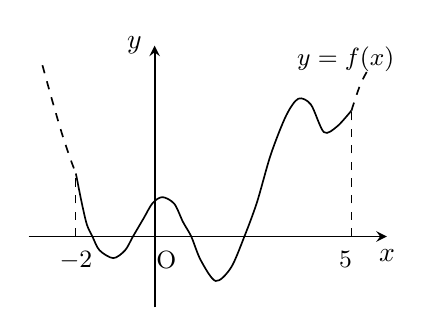
\begin{tikzpicture}[x=0.50cm, y=0.50cm, line width=0.5pt]
  \draw[->, >=stealth, line width=0.7pt] (-3.2,0) -- (5.9,0) node[below=1pt] {$x$};
  \draw[->, >=stealth, line width=0.7pt] (0,-1.8) -- (0,4.85) node[left=1pt] {$y$};
  \node[below=2pt, font=\small] at (0.3,0) {$\pt{O}$};
  % 구간 끝의 세로 안내 파선(원문)
  \draw[dashed, line width=0.35pt] (-2,0) -- (-2,1.60);
  \draw[dashed, line width=0.35pt] (5,0) -- (5,3.20);
  % 그래프 — 닫힌구간 [-2, 5] 밖은 원문처럼 파선
  \draw[dashed, line width=0.6pt, smooth] plot coordinates {(-2.85,4.35) (-2.60,3.45) (-2.35,2.60) (-2.15,2.00) (-2,1.60)};
  \draw[line width=0.6pt, smooth] plot coordinates
    {(-2,1.60) (-1.85,0.85) (-1.72,0.30) (-1.58,0) (-1.40,-0.35) (-1.05,-0.55) (-0.75,-0.35)
     (-0.55,0) (-0.28,0.46) (-0.05,0.85) (0.20,1.00) (0.50,0.83) (0.72,0.37) (0.93,0)
     (1.17,-0.60) (1.55,-1.13) (1.94,-0.79) (2.28,0) (2.60,0.87) (2.95,2.08) (3.34,3.07)
     (3.65,3.50) (3.97,3.35) (4.30,2.65) (4.64,2.80) (5,3.20)};
  \draw[dashed, line width=0.6pt, smooth] plot coordinates {(5,3.20) (5.22,3.85) (5.40,4.20)};
  \node[below=2pt, font=\small] at (-2,0) {$-2$};
  \node[below=2pt, font=\small] at (4.85,0) {$5$};
  \node[right=1pt, font=\small] at (3.3,4.5) {$y=f(x)$};
\end{tikzpicture}
}\end{minipage}\par
\dmchoicesauto{}{$2$}{$3$}{$4$}{$5$}{$6$}
}\vspace{8mm}
\vspace{3mm}\setcounter{dmproblemcount}{79}\dmpnum{57-80}{% id: 57-80
% book: 쎈B 미적분1 · 04 도함수의 활용 (1)
% section: 유형 18 평균값 정리; 그래프를 이용하는 경우
% figure: tikz:fig-57-80
% answer: 
% answer_source: 
% variant_level: 0 (원본 전사)
% 이 파일은 build.mjs 가 items.json 에서 만든다. 고칠 때는 items.json 을 고친다.
\smash{\raisebox{4.5mm}{\dmkichul{쎈B 미적분1 57쪽 80번}}}
\noindent\begin{minipage}[t]{0.58\linewidth}\vspace{0pt}\raggedright 함수 $y=f(x)$의 그래프가 오른쪽 그림과 같을 때, \par\smallskip\end{minipage}\hfill\begin{minipage}[t]{0.4\linewidth}\vspace{0pt}\centering \resizebox{\ifdim\width>\linewidth\linewidth\else\width\fi}{!}{% 57-80(57쪽) — 구간 [α, β] 에서 평균값 정리를 묻는 문항의 y=f(x) 그래프. 스캔 화질이 낮아 TikZ 로 다시 그림.
% 원문에 있는 것만: x축 위 문자 α, β · 그 두 곳의 세로 안내 파선 · 라벨 O, x, y, y=f(x) · 구간 밖은 파선.
% 눈금 숫자는 원문에 없으므로 넣지 않는다(개수를 세는 문항이라 수치를 더하면 답이 드러난다).
% 곡선은 원문 모양 그대로 지나는 점들을 재서 smooth 로 잇는다(식이 주어진 그래프가 아니다).
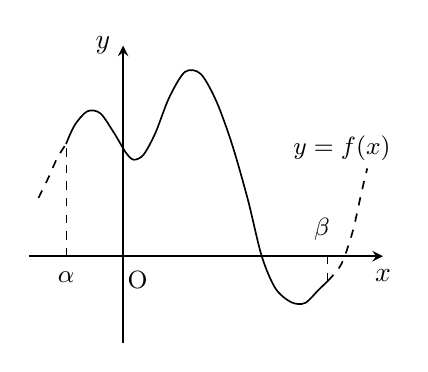
\begin{tikzpicture}[x=0.50cm, y=0.50cm, line width=0.5pt]
  \draw[->, >=stealth, line width=0.7pt] (-2.4,0) -- (6.6,0) node[below=1pt] {$x$};
  \draw[->, >=stealth, line width=0.7pt] (0,-2.2) -- (0,5.35) node[left=1pt] {$y$};
  \node[below=2pt, font=\small] at (0.37,0) {$\pt{O}$};
  % 구간 끝의 세로 안내 파선(원문: α 는 축 위로, β 는 축 아래로)
  \draw[dashed, line width=0.35pt] (-1.45,0) -- (-1.45,2.85);
  \draw[dashed, line width=0.35pt] (5.20,0) -- (5.20,-0.63);
  % 그래프 — 구간 [α, β] 밖은 원문처럼 파선
  \draw[dashed, line width=0.6pt, smooth] plot coordinates {(-2.15,1.48) (-1.88,2.03) (-1.68,2.48) (-1.45,2.85)};
  \draw[line width=0.6pt, smooth] plot coordinates
    {(-1.45,2.85) (-1.23,3.33) (-0.91,3.68) (-0.58,3.63) (-0.23,3.13) (0.07,2.63) (0.27,2.45)
     (0.52,2.58) (0.82,3.13) (1.17,4.03) (1.57,4.68) (1.97,4.63) (2.37,3.93) (2.77,2.83)
     (3.17,1.43) (3.52,0) (3.87,-0.82) (4.27,-1.17) (4.62,-1.19) (4.97,-0.85) (5.20,-0.63)};
  \draw[dashed, line width=0.6pt, smooth] plot coordinates {(5.20,-0.63) (5.47,-0.32) (5.63,0) (5.85,0.70) (6.05,1.60) (6.20,2.23)};
  \node[below=2pt, font=\small] at (-1.45,0) {$\alpha$};
  \node[above=1pt, font=\small] at (5.05,0.08) {$\beta$};
  \node[right=1pt, font=\small] at (4.0,2.75) {$y=f(x)$};
\end{tikzpicture}
}\end{minipage}\par
\noindent \dispeq{$\dfrac{f(\beta)-f(\alpha)}{\beta-\alpha}=f'(c)$}\par\smallskip\noindent 를 만족시키는 상수 $c$의 개수를 구하시오. \dmcondfill{$\alpha<c<\beta$}{}
}\vspace{8mm}
\vspace{5mm}\setcounter{dmproblemcount}{80}\dmpnum{57-81}{% id: 57-81
% book: 쎈B 미적분1 · 04 도함수의 활용 (1)
% section: 유형 18 평균값 정리; 그래프를 이용하는 경우
% figure: none
% answer: 
% answer_source: 
% variant_level: 0 (원본 전사)
% 이 파일은 build.mjs 가 items.json 에서 만든다. 고칠 때는 items.json 을 고친다.
\smash{\raisebox{6.5mm}{\dmkichul{쎈B 미적분1 57쪽 81번}}}
함수 \par\smallskip\dispeq{$f(x)=\begin{cases} x^2-4x+5 & (x\ge 1) \\ -2x^2+2x+2 & (x<1) \end{cases}$}\par\smallskip\noindent 에 대하여 닫힌구간 $[-1{,}\mkern3mu\mathopen{}4]$에서 평균값 정리를 만족시키는 상수 $c$의 개수는?
\dmchoicesauto{}{$1$}{$2$}{$3$}{$4$}{$5$}
}\vspace{8mm}
\vspace{3mm}\setcounter{dmproblemcount}{81}\dmpnum{57-82}{% id: 57-82
% book: 쎈B 미적분1 · 04 도함수의 활용 (1)
% section: 유형 18 평균값 정리; 그래프를 이용하는 경우
% figure: none
% answer: 
% answer_source: 
% variant_level: 0 (원본 전사)
% 이 파일은 build.mjs 가 items.json 에서 만든다. 고칠 때는 items.json 을 고친다.
\smash{\raisebox{4.5mm}{\dmkichul{쎈B 미적분1 57쪽 82번}}}
함수 $f(x)$에 대하여 $\dfrac{f(1)-f(-1)}{2}=f'(c)$인 상수 $c$가 열린구간 $(-1{,}\mkern3mu\mathopen{}1)$에 존재하는 함수인 것만을 보기에서 있는 대로 고른 것은? \bogi{ㄱ. $f(x)=|x+2|$\\[1.5mm] ㄴ. $f(x)=x\sqrt{x^2}$\\[3mm] ㄷ. $f(x)=\begin{cases} x^2-3x+2 & (x\ge 0) \\ x^2+2x+2 & (x<0) \end{cases}$}
\dmchoicesauto{}{ㄱ}{ㄴ}{ㄷ}{ㄱ, ㄴ}{ㄴ, ㄷ}
}\vspace{8mm}
\vspace*{0pt plus 1filll}
\clearpage
\renewcommand{\dmchapunit}{05 도함수의 활용 (2)}
\dmchapter{05}{도함수의 활용 (2)}
\setcounter{dmproblemcount}{0}
\dmsection{유형 01 함수의 증가와 감소}
\setcounter{dmproblemcount}{0}\dmpnum{59-01}{% id: 59-01
% book: 쎈B 미적분1 · 05 도함수의 활용 (2)
% section: 유형 01 함수의 증가와 감소
% figure: none
% answer: 
% answer_source: 
% variant_level: 0 (원본 전사)
% 이 파일은 build.mjs 가 items.json 에서 만든다. 고칠 때는 items.json 을 고친다.
\smash{\raisebox{1.5mm}{\dmkichul{쎈B 미적분1 59쪽 01번 · 대표 문제}}}
함수 $f(x)=-x^3-6x^2+15x+4$가 증가하는 구간은 $[\alpha{,}\mkern3mu\mathopen{}\beta]$이다. 이때 $\alpha+\beta$의 값은?
\dmchoicesauto{}{$-4$}{$-2$}{$0$}{$2$}{$4$}
}\vspace{8mm}
\setcounter{dmproblemcount}{1}\dmpnum{59-02}{% id: 59-02
% book: 쎈B 미적분1 · 05 도함수의 활용 (2)
% section: 유형 01 함수의 증가와 감소
% figure: none
% answer: 
% answer_source: 
% variant_level: 0 (원본 전사)
% 이 파일은 build.mjs 가 items.json 에서 만든다. 고칠 때는 items.json 을 고친다.
\smash{\raisebox{1.5mm}{\dmkichul{쎈B 미적분1 59쪽 02번}}}
함수 $f(x)=x^3-12x+5$가 구간 $[-a{,}\mkern3mu\mathopen{}a]$에서 감소할 때, 양수 $a$의 최댓값은?
\dmchoicesauto{}{$1$}{$2$}{$3$}{$4$}{$5$}
}\vspace{8mm}
\vspace{3mm}\setcounter{dmproblemcount}{2}\dmpnum{59-03}{% id: 59-03
% book: 쎈B 미적분1 · 05 도함수의 활용 (2)
% section: 유형 01 함수의 증가와 감소
% figure: none
% answer: 
% answer_source: 
% variant_level: 0 (원본 전사)
% 이 파일은 build.mjs 가 items.json 에서 만든다. 고칠 때는 items.json 을 고친다.
\smash{\raisebox{4.5mm}{\dmkichul{쎈B 미적분1 59쪽 03번}}}
함수 $f(x)=-\dfrac{1}{3}x^3+ax^2+bx+7$이 $-3\le x\le 1$에서 증가하고, $x\le -3$, $x\ge 1$에서 감소할 때, 상수 $a$, $b$에 대하여 $ab$의 값을 구하시오.
}\vspace{8mm}
\setcounter{dmproblemcount}{3}\dmpnum{59-04}{% id: 59-04
% book: 쎈B 미적분1 · 05 도함수의 활용 (2)
% section: 유형 01 함수의 증가와 감소
% figure: none
% answer: 
% answer_source: 
% variant_level: 0 (원본 전사)
% 이 파일은 build.mjs 가 items.json 에서 만든다. 고칠 때는 items.json 을 고친다.
\smash{\raisebox{1.5mm}{\dmkichul{쎈B 미적분1 59쪽 04번 · 서술형}}}
함수 $f(x)=3x^3+ax^2-72x+18$이 감소하는 $x$의 값의 범위가 $b\le x\le 2$일 때, $a+b$의 값을 구하시오. \dmcondfill{$a$는 상수이다.}{}
}\vspace{8mm}
\dmsection{유형 02 실수 전체의 집합에서 삼차함수가 증가 또는 감소하기 위한 조건}
\vspace{3mm}\setcounter{dmproblemcount}{4}\dmpnum{59-05}{% id: 59-05
% book: 쎈B 미적분1 · 05 도함수의 활용 (2)
% section: 유형 02 실수 전체의 집합에서 삼차함수가 증가 또는 감소하기 위한 조건
% figure: none
% answer: 
% answer_source: 
% variant_level: 0 (원본 전사)
% 이 파일은 build.mjs 가 items.json 에서 만든다. 고칠 때는 items.json 을 고친다.
\smash{\raisebox{4.5mm}{\dmkichul{쎈B 미적분1 59쪽 05번 · 대표 문제}}}
함수 $f(x)=\dfrac{1}{3}x^3+2ax^2+(a+14)x+3$이 실수 전체의 집합에서 증가하도록 하는 정수 $a$의 개수는?
\dmchoicesauto{}{$2$}{$3$}{$4$}{$5$}{$6$}
}\vspace{8mm}
\setcounter{dmproblemcount}{5}\dmpnum{59-06}{% id: 59-06
% book: 쎈B 미적분1 · 05 도함수의 활용 (2)
% section: 유형 02 실수 전체의 집합에서 삼차함수가 증가 또는 감소하기 위한 조건
% figure: none
% answer: 
% answer_source: 
% variant_level: 0 (원본 전사)
% 이 파일은 build.mjs 가 items.json 에서 만든다. 고칠 때는 items.json 을 고친다.
\smash{\raisebox{1.5mm}{\dmkichul{쎈B 미적분1 59쪽 06번}}}
함수 $f(x)=2ax^3+3x^2-x$가 구간 $(-\infty{,}\mkern3mu\mathopen{}\infty)$에서 감소하도록 하는 실수 $a$의 값의 범위는?
\begin{choicesii}{\rule[-3ex]{0pt}{8ex}$a\le-\dfrac{3}{2}$}{\rule[-3ex]{0pt}{8ex}$-\dfrac{3}{2}\le a<0$}{\rule[-3ex]{0pt}{8ex}$-\dfrac{3}{2}\le a<\dfrac{3}{2}$}{\rule[-3ex]{0pt}{8ex}$0\le a\le\dfrac{3}{2}$}{\rule[-3ex]{0pt}{8ex}$a\ge\dfrac{3}{2}$}\end{choicesii}
}\vspace{8mm}
\vspace{3mm}\setcounter{dmproblemcount}{6}\dmpnum{60-07}{% id: 60-07
% book: 쎈B 미적분1 · 05 도함수의 활용 (2)
% section: 유형 02 실수 전체의 집합에서 삼차함수가 증가 또는 감소하기 위한 조건
% figure: none
% answer: 
% answer_source: 
% variant_level: 0 (원본 전사)
% 이 파일은 build.mjs 가 items.json 에서 만든다. 고칠 때는 items.json 을 고친다.
\smash{\raisebox{4.5mm}{\dmkichul{쎈B 미적분1 60쪽 07번}}}
함수 $f(x)=\dfrac{2}{3}x^3-ax^2-2ax$가 다음 조건을 만족시키도록 하는 정수 $a$의 개수는? \exprbox{\begin{minipage}{0.96\linewidth}\raggedright 임의의 두 실수 $x_1$, $x_2$에 대하여 $x_1<x_2$이면 $f(x_1)<f(x_2)$이다.\end{minipage}}
\dmchoicesauto{}{$1$}{$2$}{$3$}{$4$}{$5$}
}\vspace{8mm}
\setcounter{dmproblemcount}{7}\dmpnum{60-08}{% id: 60-08
% book: 쎈B 미적분1 · 05 도함수의 활용 (2)
% section: 유형 02 실수 전체의 집합에서 삼차함수가 증가 또는 감소하기 위한 조건
% figure: none
% answer: 
% answer_source: 
% variant_level: 0 (원본 전사)
% 이 파일은 build.mjs 가 items.json 에서 만든다. 고칠 때는 items.json 을 고친다.
\smash{\raisebox{1.5mm}{\dmkichul{쎈B 미적분1 60쪽 08번 · 서술형}}}
실수 전체의 집합에서 정의된 함수\par\smallskip\dispeq{$f(x)=-x^3+3x^2-kx+2$}\par\smallskip\noindent 의 역함수가 존재하도록 하는 실수 $k$의 최솟값을 구하시오.
}\vspace{8mm}
\setcounter{dmproblemcount}{8}\dmpnum{60-09}{% id: 60-09
% book: 쎈B 미적분1 · 05 도함수의 활용 (2)
% section: 유형 02 실수 전체의 집합에서 삼차함수가 증가 또는 감소하기 위한 조건
% figure: none
% answer: 
% answer_source: 
% variant_level: 0 (원본 전사)
% 이 파일은 build.mjs 가 items.json 에서 만든다. 고칠 때는 items.json 을 고친다.
\smash{\raisebox{1.5mm}{\dmkichul{쎈B 미적분1 60쪽 09번}}}
실수 전체의 집합에서 정의된 함수\par\smallskip\dispeq{$f(x)=x^3-2(2-a)x^2+6ax+1$}\par\smallskip\noindent 이 다음 조건을 만족시키도록 하는 정수 $a$의 최댓값과 최솟값의 합은? \exprbox{\begin{minipage}{0.96\linewidth}\raggedright 임의의 두 실수 $x_1$, $x_2$에 대하여 $x_1\ne x_2$이면 $f(x_1)\ne f(x_2)$이다.\end{minipage}}
\dmchoicesauto{}{$8$}{$9$}{$10$}{$11$}{$12$}
}\vspace{8mm}
\setcounter{dmproblemcount}{9}\dmpnum{60-10}{% id: 60-10
% book: 쎈B 미적분1 · 05 도함수의 활용 (2)
% section: 유형 02 실수 전체의 집합에서 삼차함수가 증가 또는 감소하기 위한 조건
% figure: none
% answer: 
% answer_source: 
% variant_level: 0 (원본 전사)
% 이 파일은 build.mjs 가 items.json 에서 만든다. 고칠 때는 items.json 을 고친다.
\smash{\raisebox{1.5mm}{\dmkichul{쎈B 미적분1 60쪽 10번}}}
모든 실수 $t$에 대하여 구간 $[t{,}\mkern3mu\mathopen{}\infty)$에서 함수 $f(x)=3x^3-3ax^2+(a+6)x-a$의 최솟값이 $f(t)$가 되도록 하는 정수 $a$의 최댓값은?
\dmchoicesauto{}{$0$}{$1$}{$2$}{$3$}{$4$}
}\vspace{8mm}
\dmsection{유형 03 주어진 구간에서 삼차함수가 증가 또는 감소하기 위한 조건}
\setcounter{dmproblemcount}{10}\dmpnum{60-11}{% id: 60-11
% book: 쎈B 미적분1 · 05 도함수의 활용 (2)
% section: 유형 03 주어진 구간에서 삼차함수가 증가 또는 감소하기 위한 조건
% figure: none
% answer: 
% answer_source: 
% variant_level: 0 (원본 전사)
% 이 파일은 build.mjs 가 items.json 에서 만든다. 고칠 때는 items.json 을 고친다.
\smash{\raisebox{1.5mm}{\dmkichul{쎈B 미적분1 60쪽 11번 · 대표 문제}}}
함수 $f(x)=-x^3-2x^2+ax+3$이 $0<x<1$에서 증가하도록 하는 실수 $a$의 최솟값은?
\dmchoicesauto{}{$7$}{$8$}{$9$}{$10$}{$11$}
}\vspace{8mm}
\setcounter{dmproblemcount}{11}\dmpnum{60-12}{% id: 60-12
% book: 쎈B 미적분1 · 05 도함수의 활용 (2)
% section: 유형 03 주어진 구간에서 삼차함수가 증가 또는 감소하기 위한 조건
% figure: none
% answer: 
% answer_source: 
% variant_level: 0 (원본 전사)
% 이 파일은 build.mjs 가 items.json 에서 만든다. 고칠 때는 items.json 을 고친다.
\smash{\raisebox{1.5mm}{\dmkichul{쎈B 미적분1 60쪽 12번}}}
함수 $f(x)=x^3-3x^2+(1-4a)x$가 구간 $(0{,}\mkern3mu\mathopen{}3)$에서 감소하도록 하는 실수 $a$의 값의 범위를 구하시오.
}\vspace{8mm}
\setcounter{dmproblemcount}{12}\dmpnum{61-13}{% id: 61-13
% book: 쎈B 미적분1 · 05 도함수의 활용 (2)
% section: 유형 03 주어진 구간에서 삼차함수가 증가 또는 감소하기 위한 조건
% figure: none
% answer: 
% answer_source: 
% variant_level: 0 (원본 전사)
% 이 파일은 build.mjs 가 items.json 에서 만든다. 고칠 때는 items.json 을 고친다.
\smash{\raisebox{1.5mm}{\dmkichul{쎈B 미적분1 61쪽 13번}}}
함수 $f(x)=x^3+ax^2-8x+5$가 구간 $(-2{,}\mkern3mu\mathopen{}1)$에서 감소하도록 하는 실수 $a$의 최댓값을 $M$, 최솟값을 $m$이라 할 때, $M-m$의 값은?
\dmchoicesauto{\rule[-3ex]{0pt}{8ex}}{$\dfrac{1}{2}$}{$\dfrac{3}{2}$}{$\dfrac{5}{2}$}{$\dfrac{7}{2}$}{$\dfrac{9}{2}$}
}\vspace{8mm}
\setcounter{dmproblemcount}{13}\dmpnum{61-14}{% id: 61-14
% book: 쎈B 미적분1 · 05 도함수의 활용 (2)
% section: 유형 03 주어진 구간에서 삼차함수가 증가 또는 감소하기 위한 조건
% figure: none
% answer: 
% answer_source: 
% variant_level: 0 (원본 전사)
% 이 파일은 build.mjs 가 items.json 에서 만든다. 고칠 때는 items.json 을 고친다.
\smash{\raisebox{1.5mm}{\dmkichul{쎈B 미적분1 61쪽 14번 · 서술형}}}
함수 $f(x)=-x^3+2ax^2-3$이 구간 $(1{,}\mkern3mu\mathopen{}2)$에서 증가하고, 구간 $(3{,}\mkern3mu\mathopen{}\infty)$에서 감소하도록 하는 정수 $a$의 값을 구하시오.
}\vspace{8mm}
\setcounter{dmproblemcount}{14}\dmpnum{61-15}{% id: 61-15
% book: 쎈B 미적분1 · 05 도함수의 활용 (2)
% section: 유형 03 주어진 구간에서 삼차함수가 증가 또는 감소하기 위한 조건
% figure: none
% answer: 
% answer_source: 
% variant_level: 0 (원본 전사)
% 이 파일은 build.mjs 가 items.json 에서 만든다. 고칠 때는 items.json 을 고친다.
\smash{\raisebox{1.5mm}{\dmkichul{쎈B 미적분1 61쪽 15번}}}
함수 $f(x)=-x^3+2ax^2+(a-1)x$에 대하여 곡선 $y=f(x)$ 위의 점 $(t{,}\mkern3mu\mathopen{}f(t))$에서의 접선의 $y$절편을 $g(t)$라 하자. 함수 $g(t)$가 구간 $(-6{,}\mkern3mu\mathopen{}0)$에서 감소할 때, 실수 $a$의 최댓값은?
\dmchoicesauto{}{$-12$}{$-9$}{$-6$}{$-3$}{$0$}
}\vspace{8mm}
\dmsection{유형 04 함수의 그래프와 증가·감소}
\setcounter{dmproblemcount}{15}\dmpnum{61-16}{% id: 61-16
% book: 쎈B 미적분1 · 05 도함수의 활용 (2)
% section: 유형 04 함수의 그래프와 증가·감소
% figure: tikz:fig-61-16
% answer: 
% answer_source: 
% variant_level: 0 (원본 전사)
% 이 파일은 build.mjs 가 items.json 에서 만든다. 고칠 때는 items.json 을 고친다.
\smash{\raisebox{1.5mm}{\dmkichul{쎈B 미적분1 61쪽 16번 · 대표 문제}}}
다항함수 $f(x)$의 도함수 $y=f'(x)$의 그래프가 다음 그림과 같을 때, 옳은 것만을 보기에서 있는 대로 고른 것은? 
\par\smallskip\begin{center}\resizebox{\ifdim\width>\linewidth\linewidth\else\width\fi}{!}{% 61-16(61쪽) — 도함수 y=f'(x) 의 그래프(사차 모양 · 왼쪽 x절편은 −4 와 −3 사이 · x=0 에서 x축에 접함 · 오른쪽 x절편 3). 스캔 화질이 낮아 TikZ 로 다시 그림.
% 원문에 있는 것만: 눈금 숫자 −4 −3 −1 2 3 4 · 라벨 O, x, y, y=f'(x) · 안내 파선(−4 와 4 는 축에서 아래로 곡선까지, −3 · −1 · 2 는 축에서 위로 곡선까지).
% 눈금 −3 · −1 · 2 · 4 는 보기 ㄱ~ㄹ 의 구간 끝이고 x절편이 아니다. 원문의 왼쪽 x절편은 −4 보다 오른쪽(약 −3.7)에 있으므로 그대로 옮긴다 — 여기를 −4 로 그리면 보기 ㄱ 의 참거짓이 뒤집힌다.
% 곡선은 식이 주어진 그래프가 아니라 원문 모양을 재어 지나는 점을 smooth 로 이었다. y 값은 원문 비율만 맞춘 것이고 눈금이 없다.
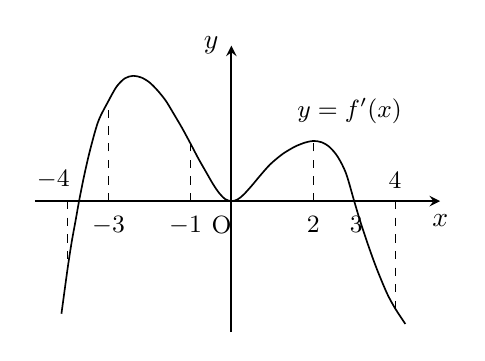
\begin{tikzpicture}[x=0.52cm, y=0.52cm, line width=0.5pt]
  \draw[->, >=stealth, line width=0.7pt] (-4.8,0) -- (5.1,0) node[below=1pt] {$x$};
  \draw[->, >=stealth, line width=0.7pt] (0,-3.2) -- (0,3.8) node[left=1pt] {$y$};
  \node[below=2pt, font=\small] at (-0.24,0) {$\pt{O}$};
  % 안내 파선(원문)
  \draw[dashed, line width=0.35pt] (-4,0) -- (-4,-1.65);
  \draw[dashed, line width=0.35pt] (-3,0) -- (-3,2.45);
  \draw[dashed, line width=0.35pt] (-1,0) -- (-1,1.41);
  \draw[dashed, line width=0.35pt] (2,0) -- (2,1.47);
  \draw[dashed, line width=0.35pt] (4,0) -- (4,-2.62);
  % 그래프
  \draw[line width=0.6pt, smooth] plot coordinates {(-4.15,-2.75) (-4.00,-1.65) (-3.90,-1.00) (-3.80,-0.45) (-3.72,0) (-3.60,0.60) (-3.45,1.25) (-3.25,1.95) (-3.00,2.45) (-2.80,2.80) (-2.60,3.00) (-2.40,3.06) (-2.20,3.02) (-2.00,2.90) (-1.80,2.70) (-1.60,2.45) (-1.40,2.12) (-1.20,1.78) (-1.00,1.41) (-0.80,1.03) (-0.60,0.68) (-0.45,0.42) (-0.30,0.20) (-0.15,0.05) (0,0) (0.15,0.04) (0.30,0.16) (0.50,0.38) (0.70,0.62) (0.95,0.90) (1.25,1.15) (1.55,1.33) (1.80,1.43) (2.00,1.47) (2.20,1.44) (2.40,1.32) (2.60,1.08) (2.80,0.68) (3.00,0) (3.15,-0.50) (3.35,-1.10) (3.55,-1.65) (3.80,-2.25) (4.00,-2.62) (4.25,-3.00)};
  % 눈금 라벨(원문 자리 그대로: −4 와 4 는 축 위, −3 · −1 · 2 · 3 은 축 아래)
  \node[above=1pt, font=\small] at (-4.35,0) {$-4$};
  \node[below=2pt, font=\small] at (-3,0) {$-3$};
  \node[below=2pt, font=\small] at (-1.12,0) {$-1$};
  \node[below=2pt, font=\small] at (2,0) {$2$};
  \node[below=2pt, font=\small] at (3.05,0) {$3$};
  \node[above=1pt, font=\small] at (4,0) {$4$};
  \node[right=1pt, font=\small] at (1.3,2.2) {$y=f'(x)$};
\end{tikzpicture}
}\end{center}
\noindent \bogi{ㄱ. $f(x)$는 구간 $(-4{,}\mkern3mu\mathopen{}-3)$에서 증가한다.\\ ㄴ. $f(x)$는 구간 $(-1{,}\mkern3mu\mathopen{}0)$에서 증가한다.\\ ㄷ. $f(x)$는 구간 $(2{,}\mkern3mu\mathopen{}3)$에서 감소한다.\\ ㄹ. $f(x)$는 구간 $(3{,}\mkern3mu\mathopen{}4)$에서 감소한다.}
\dmchoicesauto{}{ㄱ, ㄴ}{ㄱ, ㄷ}{ㄴ, ㄷ}{ㄴ, ㄹ}{ㄷ, ㄹ}
}\vspace{8mm}
\setcounter{dmproblemcount}{16}\dmpnum{61-17}{% id: 61-17
% book: 쎈B 미적분1 · 05 도함수의 활용 (2)
% section: 유형 04 함수의 그래프와 증가·감소
% figure: tikz:fig-61-17
% answer: 
% answer_source: 
% variant_level: 0 (원본 전사)
% 이 파일은 build.mjs 가 items.json 에서 만든다. 고칠 때는 items.json 을 고친다.
\smash{\raisebox{1.5mm}{\dmkichul{쎈B 미적분1 61쪽 17번}}}
\noindent\begin{minipage}[t]{0.58\linewidth}\vspace{0pt}\raggedright 이차함수 $f(x)$와 삼차함수 $g(x)$의 도함수 $y=f'(x)$, $y=g'(x)$의 그래프가 오른쪽 그림과 같을 때, 다음 중 함수 $h(x)=f(x)-g(x)$가 감소하는 구간인 것은?\end{minipage}\hfill\begin{minipage}[t]{0.4\linewidth}\vspace{0pt}\centering \resizebox{\ifdim\width>\linewidth\linewidth\else\width\fi}{!}{% 61-17(61쪽) — 이차함수 f 의 도함수 y=f'(x)(직선)와 삼차함수 g 의 도함수 y=g'(x)(아래로 볼록한 포물선). 스캔 화질이 낮아 TikZ 로 다시 그림.
% 원문에 있는 것만: x축 위 문자 a b c d e · 라벨 O, x, y, y=f'(x), y=g'(x) · 안내 파선(b 는 축에서 아래로 두 그래프의 교점까지, e 는 축에서 위로 교점까지).
% 원문의 뜻: a · d 는 포물선의 x절편, c 는 직선의 x절편, b · e 는 두 그래프의 교점의 x좌표. 순서 a<b<c<O<d<e 를 그대로 지킨다.
% 포물선 y=0.30(x+4.2)(x-1.9), 직선 y=0.51(x+1.659) 로 두면 교점이 정확히 x=-3.6(b) · x=3.0(e) 이 되어 원문 배치와 같다. 눈금은 원문에 없으므로 넣지 않는다.
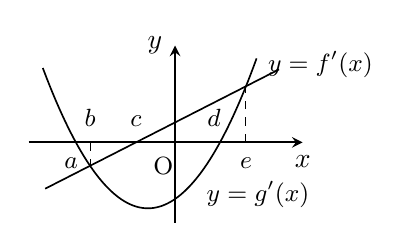
\begin{tikzpicture}[x=0.30cm, y=0.30cm, line width=0.5pt]
  \draw[->, >=stealth, line width=0.7pt] (-6.2,0) -- (5.4,0) node[below=1pt] {$x$};
  \draw[->, >=stealth, line width=0.7pt] (0,-3.4) -- (0,4.1) node[left=1pt] {$y$};
  \node[below=2pt, font=\small] at (-0.5,0) {$\pt{O}$};
  % 안내 파선(원문)
  \draw[dashed, line width=0.35pt] (-3.6,0) -- (-3.6,-0.99);
  \draw[dashed, line width=0.35pt] (3,0) -- (3,2.38);
  % 그래프
  \draw[line width=0.6pt, domain=-5.6:3.45, samples=80, smooth] plot (\x, {0.30*(\x+4.2)*(\x-1.9)});
  \draw[line width=0.6pt] (-5.5,-1.96) -- (4.4,3.09);
  % 문자(원문 자리 그대로: b · c · d 는 축 위, a · e 는 축 아래)
  \node[below=2pt, font=\small] at (-4.4,0) {$a$};
  \node[above=2pt, font=\small] at (-3.6,0) {$b$};
  \node[above=2pt, font=\small] at (-1.66,0) {$c$};
  \node[above=2pt, font=\small] at (1.65,0) {$d$};
  \node[below=2pt, font=\small] at (3,0) {$e$};
  \node[right=1pt, font=\small] at (3.4,3.3) {$y=f'(x)$};
  \node[right=1pt, font=\small] at (0.8,-2.2) {$y=g'(x)$};
\end{tikzpicture}
}\end{minipage}\par
\begin{choices32}{$(-\infty{,}\mkern3mu\mathopen{}b)$}{$(a{,}\mkern3mu\mathopen{}d)$}{$(b{,}\mkern3mu\mathopen{}c)$}{$(b{,}\mkern3mu\mathopen{}e)$}{$(d{,}\mkern3mu\mathopen{}\infty)$}\end{choices32}
}\vspace{8mm}
\setcounter{dmproblemcount}{17}\dmpnum{62-18}{% id: 62-18
% book: 쎈B 미적분1 · 05 도함수의 활용 (2)
% section: 유형 04 함수의 그래프와 증가·감소
% figure: tikz:fig-62-18
% answer: 
% answer_source: 
% variant_level: 0 (원본 전사)
% 이 파일은 build.mjs 가 items.json 에서 만든다. 고칠 때는 items.json 을 고친다.
\smash{\raisebox{1.5mm}{\dmkichul{쎈B 미적분1 62쪽 18번}}}
사차함수 $y=f(x)$의 그래프가 아래 그림과 같을 때, 다음 중 함수 $y=\{f(x)\}^2$이 증가하는 구간인 것은?
\par\smallskip\begin{center}\resizebox{\ifdim\width>\linewidth\linewidth\else\width\fi}{!}{% 62-18(62쪽) — 사차함수 y=f(x) 의 그래프(x절편 a · c · e · g, 극소 b · f, 극대 d). 스캔 화질이 낮아 TikZ 로 다시 그림.
% 원문에 있는 것만: x축 위 문자 a b c d e f g · 라벨 O, x, y, y=f(x) · 안내 파선(b 와 f 는 축에서 아래로 극솟점까지, d 는 축에서 위로 극댓점까지).
% 원문의 뜻: a · c · e · g 는 x절편, b · f 는 극소가 되는 x, d 는 극대가 되는 x. 순서 a<b<c<O<d<e<f<g 를 그대로 지킨다.
% 곡선은 식이 주어진 그래프가 아니라 원문 모양을 재어 지나는 점을 smooth 로 이었다. 눈금은 원문에 없으므로 넣지 않는다.
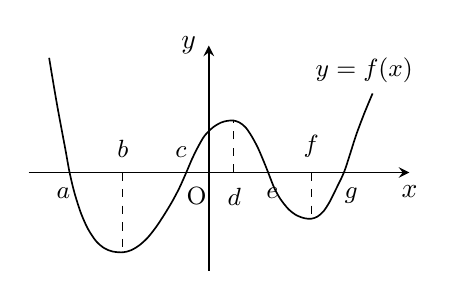
\begin{tikzpicture}[x=0.52cm, y=0.52cm, line width=0.5pt]
  \draw[->, >=stealth, line width=0.7pt] (-4.4,0) -- (4.9,0) node[below=1pt] {$x$};
  \draw[->, >=stealth, line width=0.7pt] (0,-2.4) -- (0,3.1) node[left=1pt] {$y$};
  \node[below=2pt, font=\small] at (-0.3,0) {$\pt{O}$};
  % 안내 파선(원문)
  \draw[dashed, line width=0.35pt] (-2.10,0) -- (-2.10,-1.95);
  \draw[dashed, line width=0.35pt] (0.60,0) -- (0.60,1.27);
  \draw[dashed, line width=0.35pt] (2.50,0) -- (2.50,-1.13);
  % 그래프
  \draw[line width=0.6pt, smooth] plot coordinates {(-3.90,2.80) (-3.80,2.20) (-3.70,1.62) (-3.60,1.08) (-3.50,0.55) (-3.40,0) (-3.28,-0.50) (-3.12,-1.00) (-2.95,-1.38) (-2.75,-1.68) (-2.55,-1.85) (-2.35,-1.93) (-2.10,-1.95) (-1.90,-1.90) (-1.70,-1.78) (-1.50,-1.60) (-1.30,-1.35) (-1.10,-1.05) (-0.90,-0.72) (-0.72,-0.38) (-0.55,0) (-0.40,0.35) (-0.25,0.65) (-0.10,0.90) (0.10,1.10) (0.30,1.22) (0.45,1.26) (0.60,1.27) (0.75,1.22) (0.90,1.10) (1.05,0.88) (1.20,0.60) (1.35,0.25) (1.45,0) (1.60,-0.38) (1.75,-0.65) (1.95,-0.90) (2.15,-1.05) (2.35,-1.12) (2.50,-1.13) (2.65,-1.08) (2.80,-0.95) (2.95,-0.72) (3.10,-0.42) (3.30,0) (3.45,0.45) (3.60,0.92) (3.80,1.45) (4.00,1.93)};
  % 문자(원문 자리 그대로: b · c · f 는 축 위, a · d · e · g 는 축 아래)
  \node[below=2pt, font=\small] at (-3.55,0) {$a$};
  \node[above=2pt, font=\small] at (-2.10,0) {$b$};
  \node[above=2pt, font=\small] at (-0.68,0) {$c$};
  \node[below=2pt, font=\small] at (0.62,0) {$d$};
  \node[below=2pt, font=\small] at (1.55,0) {$e$};
  \node[above=2pt, font=\small] at (2.50,0) {$f$};
  \node[below=2pt, font=\small] at (3.48,0) {$g$};
  \node[right=1pt, font=\small] at (2.3,2.5) {$y=f(x)$};
\end{tikzpicture}
}\end{center}
\begin{choices32}{$(-\infty{,}\mkern3mu\mathopen{}a)$}{$(b{,}\mkern3mu\mathopen{}c)$}{$(c{,}\mkern3mu\mathopen{}d)$}{$(d{,}\mkern3mu\mathopen{}e)$}{$(f{,}\mkern3mu\mathopen{}g)$}\end{choices32}
}\vspace{8mm}
\dmsection{유형 05 함수의 극대·극소}
\setcounter{dmproblemcount}{18}\dmpnum{62-19}{% id: 62-19
% book: 쎈B 미적분1 · 05 도함수의 활용 (2)
% section: 유형 05 함수의 극대·극소
% figure: none
% answer: 
% answer_source: 
% variant_level: 0 (원본 전사)
% 이 파일은 build.mjs 가 items.json 에서 만든다. 고칠 때는 items.json 을 고친다.
\smash{\raisebox{1.5mm}{\dmkichul{쎈B 미적분1 62쪽 19번 · 대표 문제}}}
함수 $f(x)=-x^3-3x^2+9x+10$의 극댓값과 극솟값의 합을 구하시오.
}\vspace{8mm}
\vspace{3mm}\setcounter{dmproblemcount}{19}\dmpnum{62-20}{% id: 62-20
% book: 쎈B 미적분1 · 05 도함수의 활용 (2)
% section: 유형 05 함수의 극대·극소
% figure: none
% answer: 
% answer_source: 
% variant_level: 0 (원본 전사)
% 이 파일은 build.mjs 가 items.json 에서 만든다. 고칠 때는 items.json 을 고친다.
\smash{\raisebox{4.5mm}{\dmkichul{쎈B 미적분1 62쪽 20번}}}
함수 $f(x)=\dfrac{1}{4}x^4-6x^2-16x+16$의 극댓값의 개수를 $a$, 극솟값의 개수를 $b$라 할 때, $3a+b$의 값을 구하시오.
}\vspace{8mm}
\setcounter{dmproblemcount}{20}\dmpnum{62-21}{% id: 62-21
% book: 쎈B 미적분1 · 05 도함수의 활용 (2)
% section: 유형 05 함수의 극대·극소
% figure: none
% answer: 
% answer_source: 
% variant_level: 0 (원본 전사)
% 이 파일은 build.mjs 가 items.json 에서 만든다. 고칠 때는 items.json 을 고친다.
\smash{\raisebox{1.5mm}{\dmkichul{쎈B 미적분1 62쪽 21번}}}
함수 $f(x)=x^3-3x+7$이 $x=a$에서 극대일 때, $a-f(a)$의 값을 구하시오.
}\vspace{8mm}
\setcounter{dmproblemcount}{21}\dmpnum{62-22}{% id: 62-22
% book: 쎈B 미적분1 · 05 도함수의 활용 (2)
% section: 유형 05 함수의 극대·극소
% figure: none
% answer: 
% answer_source: 
% variant_level: 0 (원본 전사)
% 이 파일은 build.mjs 가 items.json 에서 만든다. 고칠 때는 items.json 을 고친다.
\smash{\raisebox{1.5mm}{\dmkichul{쎈B 미적분1 62쪽 22번}}}
함수 $f(x)=3x^4+8x^3-6x^2-24x$의 모든 극값의 합은?
\dmchoicesauto{}{$-8$}{$-5$}{$-2$}{$2$}{$5$}
}\vspace{8mm}
\setcounter{dmproblemcount}{22}\dmpnum{62-23}{% id: 62-23
% book: 쎈B 미적분1 · 05 도함수의 활용 (2)
% section: 유형 05 함수의 극대·극소
% figure: none
% answer: 
% answer_source: 
% variant_level: 0 (원본 전사)
% 이 파일은 build.mjs 가 items.json 에서 만든다. 고칠 때는 items.json 을 고친다.
\smash{\raisebox{1.5mm}{\dmkichul{쎈B 미적분1 62쪽 23번 · 서술형}}}
함수 $f(x)=-x^4+6x^2-6$에 대하여 $y=f(x)$의 그래프에서 극대 또는 극소가 되는 세 점을 각각 $\pt{A}$, $\pt{B}$, $\pt{C}$라 하자. 이때 삼각형~$\pt{ABC}$의 넓이를 구하시오.
}\vspace{8mm}
\setcounter{dmproblemcount}{23}\dmpnum{62-24}{% id: 62-24
% book: 쎈B 미적분1 · 05 도함수의 활용 (2)
% section: 유형 05 함수의 극대·극소
% figure: none
% answer: 
% answer_source: 
% variant_level: 0 (원본 전사)
% 이 파일은 build.mjs 가 items.json 에서 만든다. 고칠 때는 items.json 을 고친다.
\smash{\raisebox{1.5mm}{\dmkichul{쎈B 미적분1 62쪽 24번}}}
실수 전체의 집합에서 정의된 다항함수 $f(x)$가 모든 실수 $x$, $y$에 대하여\par\smallskip\dispeq{$f(x+y)=f(x)+f(y)+2xy(x+y)$}\par\smallskip\noindent 를 만족시키고 $f'(0)=-2$이다. 함수 $f(x)$가 $x=\alpha$에서 극대이고, $x=\beta$에서 극소일 때, $2\alpha+5\beta$의 값을 구하시오.
}\vspace{8mm}
\dmsection{유형 06 함수의 극대·극소를 이용한 미정계수의 결정}
\setcounter{dmproblemcount}{24}\dmpnum{63-25}{% id: 63-25
% book: 쎈B 미적분1 · 05 도함수의 활용 (2)
% section: 유형 06 함수의 극대·극소를 이용한 미정계수의 결정
% figure: none
% answer: 
% answer_source: 
% variant_level: 0 (원본 전사)
% 이 파일은 build.mjs 가 items.json 에서 만든다. 고칠 때는 items.json 을 고친다.
\smash{\raisebox{1.5mm}{\dmkichul{쎈B 미적분1 63쪽 25번 · 대표 문제}}}
함수 $f(x)=x^3-3ax+b$가 $x=-2$에서 극댓값 $14$를 가질 때, 함수 $f(x)$의 극솟값은? \dmcondfill{$a$, $b$는 상수이다.}{}
\dmchoicesauto{}{$-20$}{$-18$}{$-16$}{$-14$}{$-12$}
}\vspace{8mm}
\setcounter{dmproblemcount}{25}\dmpnum{63-26}{% id: 63-26
% book: 쎈B 미적분1 · 05 도함수의 활용 (2)
% section: 유형 06 함수의 극대·극소를 이용한 미정계수의 결정
% figure: none
% answer: 
% answer_source: 
% variant_level: 0 (원본 전사)
% 이 파일은 build.mjs 가 items.json 에서 만든다. 고칠 때는 items.json 을 고친다.
\smash{\raisebox{1.5mm}{\dmkichul{쎈B 미적분1 63쪽 26번}}}
함수 $f(x)=-x^3+ax^2+bx+5$가 $x=1$에서 극소이고 $x=5$에서 극대일 때, 함수 $f(x)$의 극댓값을 구하시오. \dmcondfill{$a$, $b$는 상수이다.}{}
}\vspace{8mm}
\setcounter{dmproblemcount}{26}\dmpnum{63-27}{% id: 63-27
% book: 쎈B 미적분1 · 05 도함수의 활용 (2)
% section: 유형 06 함수의 극대·극소를 이용한 미정계수의 결정
% figure: none
% answer: 
% answer_source: 
% variant_level: 0 (원본 전사)
% 이 파일은 build.mjs 가 items.json 에서 만든다. 고칠 때는 items.json 을 고친다.
\smash{\raisebox{1.5mm}{\dmkichul{쎈B 미적분1 63쪽 27번}}}
함수 $f(x)=x^4+ax^2+b$가 $x=-3$에서 극값을 갖고, 함수 $f(x)$의 극댓값이 $8$일 때, $b-a$의 값은? \dmcondfill{$a$, $b$는 상수이다.}{}
\dmchoicesauto{}{$23$}{$24$}{$25$}{$26$}{$27$}
}\vspace{8mm}
\setcounter{dmproblemcount}{27}\dmpnum{63-28}{% id: 63-28
% book: 쎈B 미적분1 · 05 도함수의 활용 (2)
% section: 유형 06 함수의 극대·극소를 이용한 미정계수의 결정
% figure: none
% answer: 
% answer_source: 
% variant_level: 0 (원본 전사)
% 이 파일은 build.mjs 가 items.json 에서 만든다. 고칠 때는 items.json 을 고친다.
\smash{\raisebox{1.5mm}{\dmkichul{쎈B 미적분1 63쪽 28번 · 서술형}}}
함수 $f(x)=x^3+3ax^2-9a^2x$의 극댓값과 극솟값의 합이 $22$일 때, 양수 $a$의 값을 구하시오.
}\vspace{8mm}
\setcounter{dmproblemcount}{28}\dmpnum{63-29}{% id: 63-29
% book: 쎈B 미적분1 · 05 도함수의 활용 (2)
% section: 유형 06 함수의 극대·극소를 이용한 미정계수의 결정
% figure: none
% answer: 
% answer_source: 
% variant_level: 0 (원본 전사)
% 이 파일은 build.mjs 가 items.json 에서 만든다. 고칠 때는 items.json 을 고친다.
\smash{\raisebox{1.5mm}{\dmkichul{쎈B 미적분1 63쪽 29번}}}
함수 $f(x)=-x^3+3(a-1)x^2+3(-a^2+2a)x$의 극댓값이 $4$이고 $f(-2)\le 2$일 때, $f(1)$의 값은? \dmcondfill{$a$는 상수이다.}{}
\dmchoicesauto{}{$-16$}{$-14$}{$-12$}{$-10$}{$-8$}
}\vspace{8mm}
\setcounter{dmproblemcount}{29}\dmpnum{63-30}{% id: 63-30
% book: 쎈B 미적분1 · 05 도함수의 활용 (2)
% section: 유형 06 함수의 극대·극소를 이용한 미정계수의 결정
% figure: none
% answer: 
% answer_source: 
% variant_level: 0 (원본 전사)
% 이 파일은 build.mjs 가 items.json 에서 만든다. 고칠 때는 items.json 을 고친다.
\smash{\raisebox{1.5mm}{\dmkichul{쎈B 미적분1 63쪽 30번 · 서술형}}}
함수 $f(x)=x^3+ax^2+bx+c$가 다음 조건을 모두 만족시킬 때, $f(2)$의 값을 구하시오. \dmcondfill{$a$, $b$, $c$는 상수이다.}{} \exprbox{\begin{minipage}{0.96\linewidth}\raggedright ㈎ $x=1$에서 극값을 갖는다.\\[2.5mm] ㈏ $\displaystyle\lim_{x\to-3}\dfrac{f(x)}{x+3}=16$\end{minipage}}
}\vspace{8mm}
\dmsection{유형 07 함수의 극대·극소의 활용}
\vspace{3mm}\setcounter{dmproblemcount}{30}\dmpnum{64-31}{% id: 64-31
% book: 쎈B 미적분1 · 05 도함수의 활용 (2)
% section: 유형 07 함수의 극대·극소의 활용
% figure: none
% answer: 
% answer_source: 
% variant_level: 0 (원본 전사)
% 이 파일은 build.mjs 가 items.json 에서 만든다. 고칠 때는 items.json 을 고친다.
\smash{\raisebox{4.5mm}{\dmkichul{쎈B 미적분1 64쪽 31번 · 대표 문제}}}
함수 $f(x)=\dfrac{1}{9}x^3-3x+3$에 대하여 $y=f(x)$의 그래프에서 극대가 되는 점을 $\pt{A}$, 극소가 되는 점을 $\pt{B}$라 할 때, 선분~$\pt{AB}$의 중점의 좌표는?
\begin{choices32}{$(-3{,}\mkern3mu\mathopen{}0)$}{$(0{,}\mkern3mu\mathopen{}-3)$}{$(0{,}\mkern3mu\mathopen{}3)$}{$(1{,}\mkern3mu\mathopen{}3)$}{$(3{,}\mkern3mu\mathopen{}0)$}\end{choices32}
}\vspace{8mm}
\vspace{3mm}\setcounter{dmproblemcount}{31}\dmpnum{64-32}{% id: 64-32
% book: 쎈B 미적분1 · 05 도함수의 활용 (2)
% section: 유형 07 함수의 극대·극소의 활용
% figure: none
% answer: 
% answer_source: 
% variant_level: 0 (원본 전사)
% 이 파일은 build.mjs 가 items.json 에서 만든다. 고칠 때는 items.json 을 고친다.
\smash{\raisebox{4.5mm}{\dmkichul{쎈B 미적분1 64쪽 32번}}}
함수 $f(x)=-x^3+2(a-1)x^2+\dfrac{1}{3}x$는 $x=\alpha$에서 극댓값을 갖고, $x=\beta$에서 극솟값을 갖는다. 두 점~$\pt{A}(\alpha{,}\mkern3mu\mathopen{}f(\alpha))$, $\pt{B}(\beta{,}\mkern3mu\mathopen{}f(\beta))$가 원점에 대하여 대칭일 때, 상수 $a$의 값을 구하시오.
}\vspace{8mm}
\setcounter{dmproblemcount}{32}\dmpnum{64-33}{% id: 64-33
% book: 쎈B 미적분1 · 05 도함수의 활용 (2)
% section: 유형 07 함수의 극대·극소의 활용
% figure: none
% answer: 
% answer_source: 
% variant_level: 0 (원본 전사)
% 이 파일은 build.mjs 가 items.json 에서 만든다. 고칠 때는 items.json 을 고친다.
\smash{\raisebox{1.5mm}{\dmkichul{쎈B 미적분1 64쪽 33번}}}
함수 $f(x)=2x^3-3(a+2)x^2+12ax$에 대하여 곡선 $y=f(x)$가 $x$축에 접하도록 하는 실수 $a$의 값을 모두 구하시오. \dmcondfill{$a\ne 2$}{}
}\vspace{8mm}
\setcounter{dmproblemcount}{33}\dmpnum{64-34}{% id: 64-34
% book: 쎈B 미적분1 · 05 도함수의 활용 (2)
% section: 유형 07 함수의 극대·극소의 활용
% figure: none
% answer: 
% answer_source: 
% variant_level: 0 (원본 전사)
% 이 파일은 build.mjs 가 items.json 에서 만든다. 고칠 때는 items.json 을 고친다.
\smash{\raisebox{1.5mm}{\dmkichul{쎈B 미적분1 64쪽 34번}}}
함수 $f(x)=-2x^3+ax^2+48x-12$는 $x=\alpha$에서 극댓값을 갖고, $x=\beta$에서 극솟값을 갖는다. 직선 $x=a$가 두 점~$\pt{A}(\alpha{,}\mkern3mu\mathopen{}f(\alpha))$, $\pt{B}(\beta{,}\mkern3mu\mathopen{}f(\beta))$ 사이를 지날 때, 정수 $a$의 개수는?
\dmchoicesauto{}{$6$}{$7$}{$8$}{$9$}{$10$}
}\vspace{8mm}
\setcounter{dmproblemcount}{34}\dmpnum{64-35}{% id: 64-35
% book: 쎈B 미적분1 · 05 도함수의 활용 (2)
% section: 유형 07 함수의 극대·극소의 활용
% figure: none
% answer: 
% answer_source: 
% variant_level: 0 (원본 전사)
% 이 파일은 build.mjs 가 items.json 에서 만든다. 고칠 때는 items.json 을 고친다.
\smash{\raisebox{1.5mm}{\dmkichul{쎈B 미적분1 64쪽 35번 · 서술형}}}
미분가능한 함수 $f(x)$는 $x=2$에서 극솟값 $-3$을 갖는다. $g(x)=(5-2x)f(x)$라 할 때, 곡선 $y=g(x)$ 위의 $x=2$인 점에서의 접선과 $x$축, $y$축으로 둘러싸인 도형의 넓이를 구하시오.
}\vspace{8mm}
\vspace{3mm}\setcounter{dmproblemcount}{35}\dmpnum{64-36}{% id: 64-36
% book: 쎈B 미적분1 · 05 도함수의 활용 (2)
% section: 유형 07 함수의 극대·극소의 활용
% figure: none
% answer: 
% answer_source: 
% variant_level: 0 (원본 전사)
% 이 파일은 build.mjs 가 items.json 에서 만든다. 고칠 때는 items.json 을 고친다.
\smash{\raisebox{4.5mm}{\dmkichul{쎈B 미적분1 64쪽 36번}}}
함수 $f(x)=\left|\dfrac{1}{3}x^3-x^2+k\right|$가 $x=a$, $x=b$에서 극대이다. $f(a)=f(b)$일 때, 실수 $k$의 값은? \dmcondfill{$a\ne b$}{}
\dmchoicesauto{\rule[-3ex]{0pt}{8ex}}{$-\dfrac{2}{3}$}{$-\dfrac{1}{3}$}{$\dfrac{1}{3}$}{$\dfrac{2}{3}$}{$1$}
}\vspace{8mm}
\dmsection{유형 08 함수의 극대·극소를 이용한 삼차함수의 계수의 부호 결정}
\setcounter{dmproblemcount}{36}\dmpnum{65-37}{% id: 65-37
% book: 쎈B 미적분1 · 05 도함수의 활용 (2)
% section: 유형 08 함수의 극대·극소를 이용한 삼차함수의 계수의 부호 결정
% figure: tikz:fig-65-37
% answer: 
% answer_source: 
% variant_level: 0 (원본 전사)
% 이 파일은 build.mjs 가 items.json 에서 만든다. 고칠 때는 items.json 을 고친다.
\smash{\raisebox{1.5mm}{\dmkichul{쎈B 미적분1 65쪽 37번 · 대표 문제}}}
\noindent\begin{minipage}[t]{0.58\linewidth}\vspace{0pt}\raggedright 함수 $f(x)=ax^3-bx^2+cx+d$에 대하여 $y=f(x)$의 그래프가 오른쪽 그림과 같을 때, 다음 중 옳지 \underline{않은} 것은? \dmcondfill{$a$, $b$, $c$, $d$는 상수이다.}{}\end{minipage}\hfill\begin{minipage}[t]{0.4\linewidth}\vspace{0pt}\centering \resizebox{\ifdim\width>\linewidth\linewidth\else\width\fi}{!}{% 65-37(65쪽) — 삼차함수 y=f(x) 의 그래프(최고차항 음수 · 극소는 y축 왼쪽 · 극대는 y축 바로 왼쪽 · f(0)>0).
% 원문에 있는 것만: 곡선 · 라벨 y=f(x), O, x, y. 눈금·좌표는 원문에 없으므로 넣지 않는다(계수의 부호를 묻는 문항이라 수치를 더하면 답이 드러난다).
% 스캔 화질이 낮아 TikZ 로 다시 그림.
\begin{tikzpicture}[x=0.80cm, y=0.52cm, line width=0.5pt]
  \draw[->, >=stealth, line width=0.7pt] (-3.00,0) -- (1.30,0) node[below=1pt, font=\small] {$x$};
  \draw[->, >=stealth, line width=0.7pt] (0,-1.75) -- (0,2.70) node[left=1pt, font=\small] {$y$};
  % 2026-10-02 검수: 원본 x절편 비 -3.61 : -1.39 : 1 에 맞춰 근을 -1.63, -0.63, 0.45 로 다시 잡았다.
  \draw[line width=0.6pt, domain=-2.05:0.95, samples=120, smooth]
    plot (\x, {-0.8*(((\x)+1.63)*((\x)+0.63)*((\x)-0.45))});
  \node[below right=-1pt and 0pt, font=\small] at (0,0) {$\pt{O}$};
  \node[anchor=east, font=\small] at (-1.55,2.25) {$y=f(x)$};
\end{tikzpicture}
}\end{minipage}\par
\dmchoicesauto{}{$a<0$}{$b<0$}{$d>0$}{$ac>0$}{$cd<0$}
}\vspace{8mm}
\setcounter{dmproblemcount}{37}\dmpnum{65-38}{% id: 65-38
% book: 쎈B 미적분1 · 05 도함수의 활용 (2)
% section: 유형 08 함수의 극대·극소를 이용한 삼차함수의 계수의 부호 결정
% figure: tikz:fig-65-38
% answer: 
% answer_source: 
% variant_level: 0 (원본 전사)
% 이 파일은 build.mjs 가 items.json 에서 만든다. 고칠 때는 items.json 을 고친다.
\smash{\raisebox{1.5mm}{\dmkichul{쎈B 미적분1 65쪽 38번}}}
\noindent\begin{minipage}[t]{0.58\linewidth}\vspace{0pt}\raggedright 함수 $f(x)=ax^3+bx^2+cx-3$에 대하여 $y=f(x)$의 그래프가 오른쪽 그림과 같을 때, 다음 중 음수인 것은? \dmcondfill{$a$, $b$, $c$는 상수이고, $|\alpha|>|\beta|$이다.}{}\end{minipage}\hfill\begin{minipage}[t]{0.4\linewidth}\vspace{0pt}\centering \resizebox{\ifdim\width>\linewidth\linewidth\else\width\fi}{!}{% 65-38(65쪽) — 삼차함수 y=f(x) 의 그래프(최고차항 양수 · 극대의 x좌표 α · 극소의 x좌표 β · y절편 -3).
% 원문에 있는 것만: 곡선 · α·β 로 가는 세로 점선 둘 · 라벨 y=f(x), α, β, -3, O, x, y. 다른 눈금은 만들지 않는다.
% 스캔 화질이 낮아 TikZ 로 다시 그림.
\begin{tikzpicture}[x=0.72cm, y=0.44cm, line width=0.5pt]
  \draw[->, >=stealth, line width=0.7pt] (-3.05,0) -- (2.60,0) node[below=1pt, font=\small] {$x$};
  \draw[->, >=stealth, line width=0.7pt] (0,-3.25) -- (0,3.35) node[left=1pt, font=\small] {$y$};
  \draw[densely dashed, line width=0.4pt] (-1.429,0) -- (-1.429,2.56);
  \draw[densely dashed, line width=0.4pt] (0.996,0) -- (0.996,-2.78);
  \draw[line width=0.6pt, domain=-2.62:2.25, samples=140, smooth]
    plot (\x, {0.75*((\x)^3 + 0.65*(\x)^2 - 4.27*(\x) - 1.0925)});
  \node[below=1pt, font=\small] at (-1.429,0) {$\alpha$};
  \node[above=1pt, font=\small] at (0.996,0) {$\beta$};
  \node[above left=-2pt and -2pt, font=\small] at (0,0) {$\pt{O}$};
  \node[left=1pt, font=\small] at (0,-0.819) {$-3$};
  \node[anchor=west, font=\small] at (1.15,2.75) {$y=f(x)$};
\end{tikzpicture}
}\end{minipage}\par
\dmchoicesauto{}{$a+b$}{$b-c$}{$ab$}{$abc$}{$a-bc$}
}\vspace{8mm}
\vspace{3mm}\setcounter{dmproblemcount}{38}\dmpnum{65-39}{% id: 65-39
% book: 쎈B 미적분1 · 05 도함수의 활용 (2)
% section: 유형 08 함수의 극대·극소를 이용한 삼차함수의 계수의 부호 결정
% figure: tikz:fig-65-39
% answer: 
% answer_source: 
% variant_level: 0 (원본 전사)
% 이 파일은 build.mjs 가 items.json 에서 만든다. 고칠 때는 items.json 을 고친다.
\smash{\raisebox{4.5mm}{\dmkichul{쎈B 미적분1 65쪽 39번 · 서술형}}}
\noindent\begin{minipage}[t]{0.58\linewidth}\vspace{0pt}\raggedright 함수 $f(x)=-x^3+ax^2-bx+c$에 대하여 $y=f(x)$의 그래프가 오른쪽 그림과 같을 때, $\dfrac{|a|}{a}+\dfrac{2|b|}{b}+\dfrac{3|c|}{c}$의 값을 구하시오. \dmcondfill{$a$, $b$, $c$는 상수이다.}{}\end{minipage}\hfill\begin{minipage}[t]{0.4\linewidth}\vspace{0pt}\centering \resizebox{\ifdim\width>\linewidth\linewidth\else\width\fi}{!}{% 65-39(65쪽) — 삼차함수 y=f(x) 의 그래프(최고차항 음수 · 극소·극대가 모두 y축 오른쪽 · y절편 음수).
% 원문에 있는 것만: 곡선 · 라벨 y=f(x), O, x, y. 눈금은 원문에 없으므로 넣지 않는다(계수의 부호를 묻는 문항).
% 스캔 화질이 낮아 TikZ 로 다시 그림.
\begin{tikzpicture}[x=0.56cm, y=0.44cm, line width=0.5pt]
  \draw[->, >=stealth, line width=0.7pt] (-1.15,0) -- (4.75,0) node[below=1pt, font=\small] {$x$};
  \draw[->, >=stealth, line width=0.7pt] (0,-2.05) -- (0,3.15) node[left=1pt, font=\small] {$y$};
  \draw[line width=0.6pt, domain=-0.78:4.25, samples=140, smooth]
    plot (\x, {-0.55*((\x)^3 - 5.1*(\x)^2 + 4.23*(\x) + 1.755)});
  \node[below right=-1pt and -1pt, font=\small] at (0,0) {$\pt{O}$};
  \node[anchor=west, font=\small] at (2.35,2.85) {$y=f(x)$};
\end{tikzpicture}
}\end{minipage}\par
}\vspace{8mm}
\dmsection{유형 09 도함수의 그래프를 이용한 함수의 극대·극소}
\setcounter{dmproblemcount}{39}\dmpnum{65-40}{% id: 65-40
% book: 쎈B 미적분1 · 05 도함수의 활용 (2)
% section: 유형 09 도함수의 그래프를 이용한 함수의 극대·극소
% figure: tikz:fig-65-40
% answer: 
% answer_source: 
% variant_level: 0 (원본 전사)
% 이 파일은 build.mjs 가 items.json 에서 만든다. 고칠 때는 items.json 을 고친다.
\smash{\raisebox{1.5mm}{\dmkichul{쎈B 미적분1 65쪽 40번 · 대표 문제}}}
\noindent\begin{minipage}[t]{0.58\linewidth}\vspace{0pt}\raggedright 삼차함수 $f(x)=x^3+ax^2+bx+c$의 도함수 $y=f'(x)$의 그래프가 오른쪽 그림과 같다. 함수 $f(x)$의 극솟값이 $-13$일 때, $f(x)$의 극댓값을 구하시오. \dmcondfill{$a$, $b$, $c$는 상수이다.}{}\end{minipage}\hfill\begin{minipage}[t]{0.4\linewidth}\vspace{0pt}\centering \resizebox{\ifdim\width>\linewidth\linewidth\else\width\fi}{!}{% 65-40(65쪽) — 도함수 y=f'(x) 의 그래프(아래로 볼록한 포물선 · x축과 -3, 1 에서 만난다).
% 원문에 있는 것만: 곡선 · 라벨 y=f'(x), -3, O, 1, x, y. 꼭짓점 값 등 원문에 없는 눈금은 넣지 않는다.
% 스캔 화질이 낮아 TikZ 로 다시 그림.
\begin{tikzpicture}[x=0.62cm, y=0.46cm, line width=0.5pt]
  \draw[->, >=stealth, line width=0.7pt] (-4.15,0) -- (2.35,0) node[below=1pt, font=\small] {$x$};
  \draw[->, >=stealth, line width=0.7pt] (0,-2.70) -- (0,3.05) node[left=1pt, font=\small] {$y$};
  \draw[line width=0.6pt, domain=-3.85:1.85, samples=120, smooth]
    plot (\x, {0.55*((\x)+3)*((\x)-1)});
  \node[below=1pt, font=\small] at (-3,0) {$-3$};
  \node[below left=-1pt and -2pt, font=\small] at (0,0) {$\pt{O}$};
  \node[below=1pt, font=\small] at (1,0) {$1$};
  \node[anchor=east, font=\small] at (-1.85,2.60) {$y=f'(x)$};
\end{tikzpicture}
}\end{minipage}\par
}\vspace{8mm}
\setcounter{dmproblemcount}{40}\dmpnum{65-41}{% id: 65-41
% book: 쎈B 미적분1 · 05 도함수의 활용 (2)
% section: 유형 09 도함수의 그래프를 이용한 함수의 극대·극소
% figure: tikz:fig-65-41
% answer: 
% answer_source: 
% variant_level: 0 (원본 전사)
% 이 파일은 build.mjs 가 items.json 에서 만든다. 고칠 때는 items.json 을 고친다.
\smash{\raisebox{1.5mm}{\dmkichul{쎈B 미적분1 65쪽 41번}}}
함수 $f(x)$의 도함수 $y=f'(x)$의 그래프가 다음 그림과 같다. 구간 $[a{,}\mkern3mu\mathopen{}b]$에서 함수 $f(x)$가 극대가 되는 $x$의 값의 개수를 $m$, 극소가 되는 $x$의 값의 개수를 $n$이라 할 때, $m-n$의 값을 구하시오.
\par\smallskip\begin{center}\resizebox{\ifdim\width>\linewidth\linewidth\else\width\fi}{!}{% 65-41(65쪽) — 도함수 y=f'(x) 의 그래프. 구간 [a, b] 에서 x축을 아홉 번 지난다(x축 위 봉우리 4개 · 아래 골 4개).
% 원문에 있는 것만: 곡선 · a, b 로 가는 세로 점선 둘 · 라벨 a, b, O, x, y, y=f'(x). 눈금·좌표는 원문에 없으므로 넣지 않는다.
% 극대·극소의 개수를 세는 문항이므로 x축을 지나는 자리와 방향만 원문 그대로 옮긴다. 스캔 화질이 낮아 TikZ 로 다시 그림.
\begin{tikzpicture}[x=0.52cm, y=0.52cm, line width=0.5pt]
  \draw[->, >=stealth, line width=0.7pt] (-5.75,0) -- (6.35,0) node[below=1pt, font=\small] {$x$};
  \draw[->, >=stealth, line width=0.7pt] (0,-2.75) -- (0,2.35) node[left=1pt, font=\small] {$y$};
  \draw[densely dashed, line width=0.4pt] (-5.13,0) -- (-5.13,-2.33);
  \draw[densely dashed, line width=0.4pt] (5.62,0) -- (5.62,1.67);
  \draw[line width=0.6pt] plot[smooth, tension=0.6] coordinates {
    (-5.13,-2.33) (-4.90,-1.55) (-4.70,-0.60) (-4.47,0) (-4.30,0.42) (-4.13,0.45)
    (-3.95,0.30) (-3.72,0) (-3.50,-0.75) (-3.30,-1.20) (-3.13,-1.33) (-2.95,-1.15)
    (-2.80,-0.70) (-2.63,0) (-2.45,0.60) (-2.30,0.95) (-2.22,1.00) (-2.05,0.85)
    (-1.85,0.45) (-1.63,0) (-1.45,-0.90) (-1.20,-1.90) (-0.97,-2.33) (-0.75,-1.95)
    (-0.50,-1.10) (-0.22,0) (0.00,1.00) (0.20,1.65) (0.37,1.83) (0.55,1.60)
    (0.75,1.00) (1.03,0) (1.20,-0.35) (1.53,-0.42) (1.80,-0.20) (2.03,0)
    (2.20,0.55) (2.40,0.80) (2.53,0.83) (2.70,0.70) (2.88,0.35) (3.03,0)
    (3.30,-0.85) (3.60,-1.35) (4.03,-1.50) (4.40,-1.20) (4.80,-0.50) (5.20,0)
    (5.45,0.90) (5.62,1.67)};
  \node[above=1pt, font=\small] at (-5.13,0) {$a$};
  \node[below=1pt, font=\small] at (5.62,0) {$b$};
  \node[below right=-1pt and -1pt, font=\small] at (0,0) {$\pt{O}$};
  \node[anchor=west, font=\small] at (3.55,1.95) {$y=f'(x)$};
\end{tikzpicture}
}\end{center}
}\vspace{8mm}
\setcounter{dmproblemcount}{41}\dmpnum{65-42}{% id: 65-42
% book: 쎈B 미적분1 · 05 도함수의 활용 (2)
% section: 유형 09 도함수의 그래프를 이용한 함수의 극대·극소
% figure: tikz:fig-65-42
% answer: 
% answer_source: 
% variant_level: 0 (원본 전사)
% 이 파일은 build.mjs 가 items.json 에서 만든다. 고칠 때는 items.json 을 고친다.
\smash{\raisebox{1.5mm}{\dmkichul{쎈B 미적분1 65쪽 42번}}}
\noindent\begin{minipage}[t]{0.58\linewidth}\vspace{0pt}\raggedright 삼차함수 $f(x)$와 사차함수 $g(x)$의 도함수 $y=f'(x)$, $y=g'(x)$의 그래프가 오른쪽 그림과 같을 때, 다음 중 함수 $h(x)=f(x)-g(x)$가 극대가 되는 $x$의 값은?\end{minipage}\hfill\begin{minipage}[t]{0.4\linewidth}\vspace{0pt}\centering \resizebox{\ifdim\width>\linewidth\linewidth\else\width\fi}{!}{% 65-42(65쪽) — 삼차함수 f(x) 의 도함수 y=f'(x)(포물선)와 사차함수 g(x) 의 도함수 y=g'(x)(삼차곡선).
% 원문에 있는 것만: 두 곡선 · 두 곡선이 만나는 세 점(a, c, e)으로 가는 세로 점선 · 포물선이 x축과 만나는 두 점(b, d)
% · 라벨 a, b, c, d, e, O, x, y, y=f'(x), y=g'(x). 눈금·좌표는 원문에 없으므로 넣지 않는다.
% 스캔 화질이 낮아 TikZ 로 다시 그림.
\begin{tikzpicture}[x=0.56cm, y=0.50cm, line width=0.5pt]
  \draw[->, >=stealth, line width=0.7pt] (-4.10,0) -- (2.95,0) node[below=1pt, font=\small] {$x$};
  \draw[->, >=stealth, line width=0.7pt] (0,-2.75) -- (0,4.45) node[left=1pt, font=\small] {$y$};
  \draw[densely dotted, line width=0.4pt] (-3.467,0) -- (-3.467,1.09);
  \draw[densely dotted, line width=0.4pt] (-1.273,0) -- (-1.273,-1.70);
  \draw[densely dotted, line width=0.4pt] (1.424,0) -- (1.424,1.47);
  % y=f'(x) : 포물선(x축과 b, d 에서 만난다)
  \draw[line width=0.6pt, domain=-3.75:2.25, samples=120, smooth]
    plot (\x, {0.5*((\x)+2.95)*((\x)-0.75)});
  % y=g'(x) : 삼차곡선
  \draw[line width=0.6pt, domain=-3.75:2.40, samples=140, smooth]
    plot (\x, {-0.3*((\x)+3.25)*((\x)+0.4)*((\x)-2.0)});
  \node[below=1pt, font=\small] at (-3.467,0) {$a$};
  \node[above=1pt, font=\small] at (-2.95,0) {$b$};
  \node[above=1pt, font=\small] at (-1.273,0) {$c$};
  \node[above left=-2pt and -2pt, font=\small] at (0,0) {$\pt{O}$};
  \node[below=1pt, font=\small] at (0.75,0) {$d$};
  \node[below=1pt, font=\small] at (1.424,0) {$e$};
  \node[anchor=west, font=\small] at (0.45,4.05) {$y=f'(x)$};
  \node[anchor=west, font=\small] at (0.75,-2.30) {$y=g'(x)$};
\end{tikzpicture}
}\end{minipage}\par
\dmchoicesauto{}{$a$}{$b$}{$c$}{$d$}{$e$}
}\vspace{8mm}
\setcounter{dmproblemcount}{42}\dmpnum{66-43}{% id: 66-43
% book: 쎈B 미적분1 · 05 도함수의 활용 (2)
% section: 유형 09 도함수의 그래프를 이용한 함수의 극대·극소
% figure: tikz:fig-66-43
% answer: 
% answer_source: 
% variant_level: 0 (원본 전사)
% 이 파일은 build.mjs 가 items.json 에서 만든다. 고칠 때는 items.json 을 고친다.
\smash{\raisebox{1.5mm}{\dmkichul{쎈B 미적분1 66쪽 43번}}}
\noindent\begin{minipage}[t]{0.58\linewidth}\vspace{0pt}\raggedright 삼차함수 $f(x)$의 도함수 $y=f'(x)$의 그래프가 오른쪽 그림과 같을 때, 옳은 것만을 보기에서 있는 대로 고른 것은? \dmcondfill{$f(0)=0$}{}\end{minipage}\hfill\begin{minipage}[t]{0.4\linewidth}\vspace{0pt}\centering \resizebox{\ifdim\width>\linewidth\linewidth\else\width\fi}{!}{% 66-43(66쪽) — 도함수 y=f'(x) 의 그래프(아래로 볼록한 포물선 · x축과 원점, 2 에서 만난다 · 꼭짓점의 x좌표 1).
% 원문에 있는 것만: 곡선 · x=1 의 세로 점선 · 라벨 y=f'(x), O, 1, 2, x, y. 다른 눈금은 넣지 않는다.
% 스캔 화질이 낮아 TikZ 로 다시 그림.
\begin{tikzpicture}[x=0.72cm, y=0.52cm, line width=0.5pt]
  \draw[->, >=stealth, line width=0.7pt] (-0.90,0) -- (3.10,0) node[below=1pt, font=\small] {$x$};
  \draw[->, >=stealth, line width=0.7pt] (0,-1.35) -- (0,1.95) node[left=1pt, font=\small] {$y$};
  \draw[densely dashed, line width=0.4pt] (1,0) -- (1,-0.9);
  \draw[line width=0.6pt, domain=-0.55:2.60, samples=110, smooth]
    plot (\x, {0.9*(\x)*((\x)-2)});
  \node[below left=-1pt and -2pt, font=\small] at (0,0) {$\pt{O}$};
  \node[above=1pt, font=\small] at (1,0) {$1$};
  \node[below=1pt, font=\small] at (2,0) {$2$};
  \node[anchor=west, font=\small] at (1.30,1.70) {$y=f'(x)$};
\end{tikzpicture}
}\end{minipage}\par
\noindent \bogi{ㄱ. $f(x)$의 극댓값은 $0$이다.\\ ㄴ. $f(x)$는 $x=1$에서 극솟값을 갖는다.\\ ㄷ. $f(1)f(2)>0$}
\dmchoicesauto{}{ㄱ}{ㄴ}{ㄷ}{ㄱ, ㄴ}{ㄱ, ㄷ}
}\vspace{8mm}
\setcounter{dmproblemcount}{43}\dmpnum{66-44}{% id: 66-44
% book: 쎈B 미적분1 · 05 도함수의 활용 (2)
% section: 유형 09 도함수의 그래프를 이용한 함수의 극대·극소
% figure: tikz:fig-66-44
% answer: 
% answer_source: 
% variant_level: 0 (원본 전사)
% 이 파일은 build.mjs 가 items.json 에서 만든다. 고칠 때는 items.json 을 고친다.
\smash{\raisebox{1.5mm}{\dmkichul{쎈B 미적분1 66쪽 44번 · 서술형}}}
\noindent\begin{minipage}[t]{0.58\linewidth}\vspace{0pt}\raggedright 삼차함수 $f(x)=ax^3+bx^2+cx+d$의 도함수 $y=f'(x)$의 그래프가 오른쪽 그림과 같다. $f(x)$의 극댓값이 $9$이고 극솟값이 $5$일 때, $f(2)$의 값을 구하시오. \dmcondfill{$a$, $b$, $c$, $d$는 상수이다.}{}\end{minipage}\hfill\begin{minipage}[t]{0.4\linewidth}\vspace{0pt}\centering \resizebox{\ifdim\width>\linewidth\linewidth\else\width\fi}{!}{% 66-44(66쪽) — 도함수 y=f'(x) 의 그래프(아래로 볼록한 포물선 · x축과 -1, 1 에서 만난다).
% 원문에 있는 것만: 곡선 · 라벨 y=f'(x), -1, O, 1, x, y. 꼭짓점 값 등 원문에 없는 눈금은 넣지 않는다.
% 스캔 화질이 낮아 TikZ 로 다시 그림.
\begin{tikzpicture}[x=0.86cm, y=0.46cm, line width=0.5pt]
  \draw[->, >=stealth, line width=0.7pt] (-2.05,0) -- (2.10,0) node[below=1pt, font=\small] {$x$};
  \draw[->, >=stealth, line width=0.7pt] (0,-1.75) -- (0,2.55) node[left=1pt, font=\small] {$y$};
  \draw[line width=0.6pt, domain=-1.65:1.65, samples=110, smooth]
    plot (\x, {1.2*((\x)*(\x)-1)});
  \node[below=1pt, font=\small] at (-1,0) {$-1$};
  \node[below=1pt, font=\small] at (0,0) {$\pt{O}$};
  \node[below=1pt, font=\small] at (1,0) {$1$};
  \node[anchor=west, font=\small] at (0.35,2.25) {$y=f'(x)$};
\end{tikzpicture}
}\end{minipage}\par
}\vspace{8mm}
\setcounter{dmproblemcount}{44}\dmpnum{66-45}{% id: 66-45
% book: 쎈B 미적분1 · 05 도함수의 활용 (2)
% section: 유형 09 도함수의 그래프를 이용한 함수의 극대·극소
% figure: tikz:fig-66-45
% answer: 
% answer_source: 
% variant_level: 0 (원본 전사)
% 이 파일은 build.mjs 가 items.json 에서 만든다. 고칠 때는 items.json 을 고친다.
\smash{\raisebox{1.5mm}{\dmkichul{쎈B 미적분1 66쪽 45번}}}
\noindent\begin{minipage}[t]{0.58\linewidth}\vspace{0pt}\raggedright 삼차함수 $f(x)$의 도함수 $y=f'(x)$의 그래프가 오른쪽 그림과 같고, 함수 $y=f(x)$의 그래프가 점~$(0{,}\mkern3mu\mathopen{}1)$을 지날 때, $f(x)$의 극댓값과 극솟값의 합을 구하시오.\end{minipage}\hfill\begin{minipage}[t]{0.4\linewidth}\vspace{0pt}\centering \resizebox{\ifdim\width>\linewidth\linewidth\else\width\fi}{!}{% 66-45(66쪽) — 도함수 y=f'(x) 의 그래프(위로 볼록한 포물선 · x축과 -3, 1 에서 만나고 y절편 3).
% 원문에 있는 것만: 곡선 · 라벨 y=f'(x), 3, -3, O, 1, x, y. 다른 눈금은 넣지 않는다.
% 스캔 화질이 낮아 TikZ 로 다시 그림.
\begin{tikzpicture}[x=0.62cm, y=0.38cm, line width=0.5pt]
  \draw[->, >=stealth, line width=0.7pt] (-4.05,0) -- (2.15,0) node[below=1pt, font=\small] {$x$};
  \draw[->, >=stealth, line width=0.7pt] (0,-3.30) -- (0,5.15) node[left=1pt, font=\small] {$y$};
  \draw[line width=0.6pt, domain=-3.60:1.60, samples=120, smooth]
    plot (\x, {-((\x)+3)*((\x)-1)});
  \node[below=1pt, font=\small] at (-3,0) {$-3$};
  \node[below left=-1pt and -2pt, font=\small] at (0,0) {$\pt{O}$};
  \node[below=1pt, font=\small] at (1,0) {$1$};
  \node[right=1pt, font=\small] at (0,3) {$3$};
  \node[anchor=east, font=\small] at (-1.35,4.35) {$y=f'(x)$};
\end{tikzpicture}
}\end{minipage}\par
}\vspace{8mm}
\dmsection{유형 10 도함수의 그래프의 해석 (1)}
\setcounter{dmproblemcount}{45}\dmpnum{66-46}{% id: 66-46
% book: 쎈B 미적분1 · 05 도함수의 활용 (2)
% section: 유형 10 도함수의 그래프의 해석 (1)
% figure: tikz:fig-66-46
% answer: 
% answer_source: 
% variant_level: 0 (원본 전사)
% 이 파일은 build.mjs 가 items.json 에서 만든다. 고칠 때는 items.json 을 고친다.
\smash{\raisebox{1.5mm}{\dmkichul{쎈B 미적분1 66쪽 46번 · 대표 문제}}}
함수 $f(x)$의 도함수 $y=f'(x)$의 그래프가 아래 그림과 같을 때, 다음 중 옳은 것은?
\par\smallskip\begin{center}\resizebox{\ifdim\width>\linewidth\linewidth\else\width\fi}{!}{% 66-46(66쪽) — 도함수 y=f'(x) 의 그래프. x축과 0, 2, 5 에서 만나고 x=1 에서 극소 · x=4 에서 극대.
% 원문에 있는 것만: 곡선 · x=-1, 1, 3, 4, 6 의 세로 점선 · 라벨 -1, O, 1, 2, 3, 4, 5, 6, x, y, y=f'(x).
% y축 눈금은 원문에 없으므로 넣지 않는다. 스캔 화질이 낮아 TikZ 로 다시 그림.
\begin{tikzpicture}[x=0.60cm, y=0.52cm, line width=0.5pt]
  \draw[->, >=stealth, line width=0.7pt] (-2.10,0) -- (7.15,0) node[below=1pt, font=\small] {$x$};
  \draw[->, >=stealth, line width=0.7pt] (0,-2.35) -- (0,2.65) node[left=1pt, font=\small] {$y$};
  \draw[densely dashed, line width=0.4pt] (-1,0) -- (-1,1.85);
  \draw[densely dashed, line width=0.4pt] (1,0) -- (1,-0.78);
  \draw[densely dashed, line width=0.4pt] (3,0) -- (3,1.25);
  \draw[densely dashed, line width=0.4pt] (4,0) -- (4,1.63);
  \draw[densely dashed, line width=0.4pt] (6,0) -- (6,-1.40);
  \draw[line width=0.6pt] plot[smooth, tension=0.7] coordinates {
    (-1.60,2.20) (-1.30,2.05) (-1.00,1.85) (-0.70,1.45) (-0.35,0.80) (0,0)
    (0.35,-0.45) (0.70,-0.71) (1.00,-0.78) (1.30,-0.70) (1.65,-0.43) (2.00,0)
    (2.40,0.55) (2.70,0.93) (3.00,1.25) (3.40,1.50) (3.70,1.60) (4.00,1.63)
    (4.30,1.55) (4.60,1.25) (4.80,0.80) (5.00,0) (5.25,-0.70) (5.50,-1.08)
    (5.80,-1.32) (6.00,-1.40) (6.40,-1.52) (6.65,-1.58)};
  \node[below=1pt, font=\small] at (-1,0) {$-1$};
  \node[below left=-1pt and -2pt, font=\small] at (0,0) {$\pt{O}$};
  \node[above=1pt, font=\small] at (1,0) {$1$};
  \node[below=1pt, font=\small] at (2,0) {$2$};
  \node[below=1pt, font=\small] at (3,0) {$3$};
  \node[below=1pt, font=\small] at (4,0) {$4$};
  \node[below=1pt, font=\small] at (5,0) {$5$};
  \node[above=1pt, font=\small] at (6,0) {$6$};
  \node[font=\small] at (3.70,2.35) {$y=f'(x)$};
\end{tikzpicture}
}\end{center}
\par\medskip\par\noindent\hangindent=1.4em\hangafter=1 {\small ①}\ $f(x)$는 구간 $(-1{,}\mkern3mu\mathopen{}0)$에서 감소한다.\par\noindent\hangindent=1.4em\hangafter=1 {\small ②}\ $f(x)$는 구간 $(1{,}\mkern3mu\mathopen{}3)$에서 증가한다.\par\noindent\hangindent=1.4em\hangafter=1 {\small ③}\ $f(x)$는 $x=0$에서 미분가능하지 않다.\par\noindent\hangindent=1.4em\hangafter=1 {\small ④}\ $f(x)$는 $x=2$에서 극소이다.\par\noindent\hangindent=1.4em\hangafter=1 {\small ⑤}\ $f(x)$는 $x=4$에서 극대이다.\par\medskip
}\vspace{8mm}
\setcounter{dmproblemcount}{46}\dmpnum{66-47}{% id: 66-47
% book: 쎈B 미적분1 · 05 도함수의 활용 (2)
% section: 유형 10 도함수의 그래프의 해석 (1)
% figure: tikz:fig-66-47
% answer: 
% answer_source: 
% variant_level: 0 (원본 전사)
% 이 파일은 build.mjs 가 items.json 에서 만든다. 고칠 때는 items.json 을 고친다.
\smash{\raisebox{1.5mm}{\dmkichul{쎈B 미적분1 66쪽 47번}}}
함수 $f(x)$의 도함수 $y=f'(x)$의 그래프가 다음 그림과 같을 때, 옳은 것만을 보기에서 있는 대로 고르시오. \dmcondfill{$f(1)=0$}{}
\par\smallskip\begin{center}\resizebox{\ifdim\width>\linewidth\linewidth\else\width\fi}{!}{% 66-47(66쪽) — 도함수 y=f'(x) 의 그래프. x축과 -3, 1 에서 만나고 x=3 에서 x축에 접한다. x=-1 에서 극소.
% 원문에 있는 것만: 곡선 · x=-4, -1, 4 의 세로 점선 · -3 라벨에서 교점으로 가는 짧은 지시선
% · 라벨 -4, -3, -1, O, 1, 3, 4, x, y, y=f'(x). y축 눈금은 원문에 없으므로 넣지 않는다.
% 스캔 화질이 낮아 TikZ 로 다시 그림.
\begin{tikzpicture}[x=0.60cm, y=0.44cm, line width=0.5pt]
  \draw[->, >=stealth, line width=0.7pt] (-4.85,0) -- (4.95,0) node[below=1pt, font=\small] {$x$};
  \draw[->, >=stealth, line width=0.7pt] (0,-3.15) -- (0,4.25) node[left=1pt, font=\small] {$y$};
  \draw[densely dashed, line width=0.4pt] (-4,0) -- (-4,3.30);
  \draw[densely dashed, line width=0.4pt] (-1,0) -- (-1,-2.50);
  \draw[densely dashed, line width=0.4pt] (4,0) -- (4,3.30);
  \draw[line width=0.6pt] plot[smooth, tension=0.7] coordinates {
    (-4.00,3.30) (-3.75,2.40) (-3.50,1.50) (-3.25,0.70) (-3.00,0) (-2.70,-0.75)
    (-2.40,-1.35) (-2.00,-1.95) (-1.60,-2.30) (-1.30,-2.45) (-1.00,-2.50)
    (-0.70,-2.45) (-0.40,-2.30) (0,-1.95) (0.40,-1.45) (0.70,-0.85) (1.00,0)
    (1.30,0.55) (1.60,0.90) (1.90,1.10) (2.15,1.15) (2.40,1.00) (2.60,0.70)
    (2.80,0.28) (3.00,0) (3.20,0.28) (3.40,0.70) (3.65,1.55) (3.85,2.45) (4.00,3.30)};
  \draw[line width=0.4pt] (-2.72,0.62) -- (-3.00,0.04);
  \node[below=1pt, font=\small] at (-4,0) {$-4$};
  \node[anchor=south west, inner sep=1pt, font=\small] at (-2.80,0.60) {$-3$};
  \node[above=1pt, font=\small] at (-1,0) {$-1$};
  \node[below right=-1pt and -2pt, font=\small] at (0,0) {$\pt{O}$};
  \node[below=1pt, font=\small] at (1,0) {$1$};
  \node[below=1pt, font=\small] at (3,0) {$3$};
  \node[below=1pt, font=\small] at (4,0) {$4$};
  \node[anchor=west, font=\small] at (2.35,3.85) {$y=f'(x)$};
\end{tikzpicture}
}\end{center}
\noindent \bogi{ㄱ. $f(x)$는 $x=1$에서 극솟값을 갖는다.\\ ㄴ. $f(x)$는 구간 $(-1{,}\mkern3mu\mathopen{}1)$에서 증가한다.\\ ㄷ. $y=f(x)$의 그래프는 $x=1$에서 $x$축에 접한다.\\ ㄹ. 구간 $(-4{,}\mkern3mu\mathopen{}4)$에서 $f(x)$가 극댓값을 갖는 $x$의 값은 $2$개이다.}
}\vspace{8mm}
\setcounter{dmproblemcount}{47}\dmpnum{67-48}{% id: 67-48
% book: 쎈B 미적분1 · 05 도함수의 활용 (2)
% section: 유형 10 도함수의 그래프의 해석 (1)
% figure: tikz:fig-67-48
% answer: 
% answer_source: 
% variant_level: 0 (원본 전사)
% 이 파일은 build.mjs 가 items.json 에서 만든다. 고칠 때는 items.json 을 고친다.
\smash{\raisebox{1.5mm}{\dmkichul{쎈B 미적분1 67쪽 48번}}}
\noindent\begin{minipage}[t]{0.58\linewidth}\vspace{0pt}\raggedright 함수 $f(x)$의 도함수 $y=f'(x)$의 그래프가 오른쪽 그림과 같을 때, 다음 중 옳은 것은?\end{minipage}\hfill\begin{minipage}[t]{0.4\linewidth}\vspace{0pt}\centering \resizebox{\ifdim\width>\linewidth\linewidth\else\width\fi}{!}{% 67-48(67쪽) — 도함수 y=f'(x) 의 그래프(꺾은선). -1 에서 시작해 원점을 지나 1~3 에서 수평, 4 에서 x축에 닿았다가
% 5 에서 꼭짓점, 6 에서 x축을 지나 7 까지 내려간다.
% 원문에 있는 것만: 꺾은선 · x=-1, 1, 3, 5, 7 의 세로 점선 · 라벨 -1, O, 1, 3, 4, 5, 6, 7, x, y, y=f'(x).
% y축 눈금은 원문에 없으므로 넣지 않는다. 스캔 화질이 낮아 TikZ 로 다시 그림.
\begin{tikzpicture}[x=0.44cm, y=0.40cm, line width=0.5pt]
  \draw[->, >=stealth, line width=0.7pt] (-1.85,0) -- (8.10,0) node[below=1pt, font=\small] {$x$};
  \draw[->, >=stealth, line width=0.7pt] (0,-3.35) -- (0,3.45) node[left=1pt, font=\small] {$y$};
  \draw[densely dashed, line width=0.4pt] (-1,0) -- (-1,-1.13);
  \draw[densely dashed, line width=0.4pt] (1,0) -- (1,1.13);
  \draw[densely dashed, line width=0.4pt] (3,0) -- (3,1.13);
  \draw[densely dashed, line width=0.4pt] (5,0) -- (5,2.60);
  \draw[densely dashed, line width=0.4pt] (7,0) -- (7,-2.60);
  \draw[line width=0.6pt] (-1,-1.13) -- (1,1.13) -- (3,1.13) -- (4,0) -- (5,2.60) -- (7,-2.60);
  \node[above=1pt, font=\small] at (-1,0) {$-1$};
  \node[below right=-1pt and -3pt, font=\small] at (0,0) {$\pt{O}$};
  \node[below=1pt, font=\small] at (1,0) {$1$};
  \node[below=1pt, font=\small] at (3,0) {$3$};
  \node[below=1pt, font=\small] at (4,0) {$4$};
  \node[below=1pt, font=\small] at (5,0) {$5$};
  \node[below=1pt, font=\small] at (6,0) {$6$};
  \node[above=1pt, font=\small] at (7,0) {$7$};
  \node[anchor=south, font=\small] at (4.30,2.85) {$y=f'(x)$};
\end{tikzpicture}
}\end{minipage}\par
\begin{choicesv}{$-1<x<7$일 때, $f(x)$는 $3$개의 극값을 갖는다.}{$f(x)$는 $x=4$에서 극솟값을 갖는다.}{$1<x<3$에서 $f(x)$는 상수함수이다.}{$f(x)$는 $x=5$에서 미분가능하지 않다.}{$0<x<6$일 때, $f(x)$는 증가한다.}\end{choicesv}
}\vspace{8mm}
\dmsection{유형 11 도함수의 그래프의 해석 (2)}
\setcounter{dmproblemcount}{48}\dmpnum{67-49}{% id: 67-49
% book: 쎈B 미적분1 · 05 도함수의 활용 (2)
% section: 유형 11 도함수의 그래프의 해석 (2)
% figure: tikz:fig-67-49
% answer: 
% answer_source: 
% variant_level: 0 (원본 전사)
% 이 파일은 build.mjs 가 items.json 에서 만든다. 고칠 때는 items.json 을 고친다.
\smash{\raisebox{1.5mm}{\dmkichul{쎈B 미적분1 67쪽 49번 · 대표 문제}}}
\noindent\begin{minipage}[t]{0.58\linewidth}\vspace{0pt}\raggedright 다항함수 $f(x)$의 도함수 $y=f'(x)$의 그래프가 오른쪽 그림과 같을 때, 다음 중 함수 $y=f(x)$의 그래프의 개형이 될 수 있는 것은?\end{minipage}\hfill\begin{minipage}[t]{0.4\linewidth}\vspace{0pt}\centering \resizebox{\ifdim\width>\linewidth\linewidth\else\width\fi}{!}{% 67-49(67쪽) — 도함수 y=f'(x) 의 그래프. x축과 -1 에서 만나고 x=1 에서 x축에 접한다(최고차항 음수).
% 원문에 있는 것만: 곡선 · 라벨 y=f'(x), -1, O, 1, x, y. y축 눈금은 원문에 없으므로 넣지 않는다.
% 스캔 화질이 낮아 TikZ 로 다시 그림.
\begin{tikzpicture}[x=0.74cm, y=0.46cm, line width=0.5pt]
  \draw[->, >=stealth, line width=0.7pt] (-1.85,0) -- (2.20,0) node[below=1pt, font=\small] {$x$};
  \draw[->, >=stealth, line width=0.7pt] (0,-2.25) -- (0,3.40) node[left=1pt, font=\small] {$y$};
  \draw[line width=0.6pt, domain=-1.50:1.90, samples=130, smooth]
    plot (\x, {-0.8*((\x)^3 - (\x)^2 - (\x) + 1)});
  \node[below=1pt, font=\small] at (-1,0) {$-1$};
  \node[below right=-1pt and -1pt, font=\small] at (0,0) {$\pt{O}$};
  \node[above=1pt, font=\small] at (1,0) {$1$};
  \node[anchor=east, font=\small] at (-0.55,3.05) {$y=f'(x)$};
\end{tikzpicture}
}\end{minipage}\par
\begin{choicesii}{% 67-49 ①(67쪽) — 보기 그래프: x=-1 에서 극소, x=1 에서 접선이 수평인 사차함수의 개형.
% 그림 자체가 보기라 TikZ 로 다시 그림. 라벨은 원문 그대로 -1 · O · 1 · x · y 만.
\begin{tikzpicture}[x=0.50cm, y=0.50cm, line width=0.5pt, baseline=(current bounding box.center)]
  \path (-2.45,-1.25) rectangle (2.55,3.15);
  \draw[->, >=stealth, line width=0.7pt] (-2.25,0) -- (2.35,0) node[below=1pt, font=\small] {$x$};
  \draw[->, >=stealth, line width=0.7pt] (0,-0.95) -- (0,2.95) node[left=1pt, font=\small] {$y$};
  \draw[densely dashed, line width=0.4pt] (-1,0) -- (-1,-0.467);
  \draw[densely dashed, line width=0.4pt] (1,0) -- (1,0.867);
  \draw[line width=0.6pt, domain=-1.95:2.00, samples=130, smooth]
    plot (\x, {0.25*(\x)^4 - (\x)^3/3 - 0.5*(\x)^2 + (\x) + 0.45});
  \node[above=1pt, font=\small] at (-1,0) {$-1$};
  \node[below left=-2pt and -3pt, font=\small] at (0,0) {$\pt{O}$};
  \node[below=1pt, font=\small] at (1,0) {$1$};
\end{tikzpicture}
}{% 67-49 ②(67쪽) — 보기 그래프: x=-1 에서 접선이 수평이고 x=1 에서 극소인 사차함수의 개형.
% 그림 자체가 보기라 TikZ 로 다시 그림. 라벨은 원문 그대로 -1 · O · 1 · x · y 만.
\begin{tikzpicture}[x=0.50cm, y=0.50cm, line width=0.5pt, baseline=(current bounding box.center)]
  \path (-2.45,-1.25) rectangle (2.55,3.15);
  \draw[->, >=stealth, line width=0.7pt] (-2.30,0) -- (2.30,0) node[below=1pt, font=\small] {$x$};
  \draw[->, >=stealth, line width=0.7pt] (0,-0.95) -- (0,2.95) node[left=1pt, font=\small] {$y$};
  \draw[densely dashed, line width=0.4pt] (-1,0) -- (-1,0.867);
  \draw[densely dashed, line width=0.4pt] (1,0) -- (1,-0.467);
  \draw[line width=0.6pt, domain=-2.00:1.95, samples=130, smooth]
    plot (\x, {0.25*(\x)^4 + (\x)^3/3 - 0.5*(\x)^2 - (\x) + 0.45});
  \node[below=1pt, font=\small] at (-1,0) {$-1$};
  \node[below right=-2pt and -3pt, font=\small] at (0,0) {$\pt{O}$};
  \node[above=1pt, font=\small] at (1,0) {$1$};
\end{tikzpicture}
}{% 67-49 ③(67쪽) — 보기 그래프: x=-1 에서 접선이 수평이고 x=1 에서 극대인 사차함수의 개형.
% 그림 자체가 보기라 TikZ 로 다시 그림. 라벨은 원문 그대로 -1 · O · 1 · x · y 만.
\begin{tikzpicture}[x=0.50cm, y=0.50cm, line width=0.5pt, baseline=(current bounding box.center)]
  \path (-2.45,-1.45) rectangle (2.55,2.15);
  \draw[->, >=stealth, line width=0.7pt] (-2.25,0) -- (2.25,0) node[below=1pt, font=\small] {$x$};
  \draw[->, >=stealth, line width=0.7pt] (0,-1.25) -- (0,2.00) node[left=1pt, font=\small] {$y$};
  \draw[densely dashed, line width=0.4pt] (-1,0) -- (-1,0.333);
  \draw[densely dashed, line width=0.4pt] (1,0) -- (1,1.667);
  \draw[line width=0.6pt, domain=-1.90:1.90, samples=130, smooth]
    plot (\x, {-(0.25*(\x)^4 + (\x)^3/3 - 0.5*(\x)^2 - (\x)) + 0.75});
  \node[below=1pt, font=\small] at (-1,0) {$-1$};
  \node[below right=-2pt and -3pt, font=\small] at (0,0) {$\pt{O}$};
  \node[below=1pt, font=\small] at (1,0) {$1$};
\end{tikzpicture}
}{% 67-49 ④(67쪽) — 보기 그래프: x=-1 에서 극대이고 x=1 에서 접선이 수평인 사차함수의 개형.
% 그림 자체가 보기라 TikZ 로 다시 그림. 라벨은 원문 그대로 -1 · O · 1 · x · y 만.
\begin{tikzpicture}[x=0.50cm, y=0.50cm, line width=0.5pt, baseline=(current bounding box.center)]
  \path (-2.45,-1.45) rectangle (2.55,2.15);
  \draw[->, >=stealth, line width=0.7pt] (-2.25,0) -- (2.30,0) node[below=1pt, font=\small] {$x$};
  \draw[->, >=stealth, line width=0.7pt] (0,-1.25) -- (0,2.00) node[left=1pt, font=\small] {$y$};
  \draw[densely dashed, line width=0.4pt] (-1,0) -- (-1,1.667);
  \draw[densely dashed, line width=0.4pt] (1,0) -- (1,0.333);
  \draw[line width=0.6pt, domain=-1.90:1.95, samples=130, smooth]
    plot (\x, {-(0.25*(\x)^4 - (\x)^3/3 - 0.5*(\x)^2 + (\x)) + 0.75});
  \node[below=1pt, font=\small] at (-1,0) {$-1$};
  \node[below right=-2pt and -3pt, font=\small] at (0,0) {$\pt{O}$};
  \node[below=1pt, font=\small] at (1,0) {$1$};
\end{tikzpicture}
}{% 67-49 ⑤(67쪽) — 보기 그래프: x=-1 과 x=1 에서 극대, x=0 에서 극소인 사차함수의 개형.
% 그림 자체가 보기라 TikZ 로 다시 그림. 라벨은 원문 그대로 -1 · O · 1 · x · y 만.
\begin{tikzpicture}[x=0.50cm, y=0.50cm, line width=0.5pt, baseline=(current bounding box.center)]
  \path (-2.45,-1.55) rectangle (2.55,1.55);
  \draw[->, >=stealth, line width=0.7pt] (-2.20,0) -- (2.20,0) node[below=1pt, font=\small] {$x$};
  \draw[->, >=stealth, line width=0.7pt] (0,-1.35) -- (0,1.40) node[left=1pt, font=\small] {$y$};
  \draw[densely dashed, line width=0.4pt] (-1,0) -- (-1,0.85);
  \draw[densely dashed, line width=0.4pt] (1,0) -- (1,0.85);
  \draw[line width=0.6pt, domain=-1.80:1.80, samples=130, smooth]
    plot (\x, {-1.6*(0.25*(\x)^4 - 0.5*(\x)^2) + 0.45});
  \node[below=1pt, font=\small] at (-1,0) {$-1$};
  \node[below right=-2pt and -3pt, font=\small] at (0,0) {$\pt{O}$};
  \node[below=1pt, font=\small] at (1,0) {$1$};
\end{tikzpicture}
}\end{choicesii}
}\vspace{8mm}
\setcounter{dmproblemcount}{49}\dmpnum{67-50}{% id: 67-50
% book: 쎈B 미적분1 · 05 도함수의 활용 (2)
% section: 유형 11 도함수의 그래프의 해석 (2)
% figure: tikz:fig-67-50
% answer: 
% answer_source: 
% variant_level: 0 (원본 전사)
% 이 파일은 build.mjs 가 items.json 에서 만든다. 고칠 때는 items.json 을 고친다.
\smash{\raisebox{1.5mm}{\dmkichul{쎈B 미적분1 67쪽 50번}}}
\noindent\begin{minipage}[t]{0.58\linewidth}\vspace{0pt}\raggedright 함수 $f(x)$의 도함수 $y=f'(x)$의 그래프가 오른쪽 그림과 같을 때, 다음 중 함수 $y=f(x)$의 그래프의 개형이 될 수 있는 것은?\end{minipage}\hfill\begin{minipage}[t]{0.4\linewidth}\vspace{0pt}\centering \resizebox{\ifdim\width>\linewidth\linewidth\else\width\fi}{!}{% 67-50(67쪽) — 도함수 y=f'(x) 의 그래프. x축과 a, c 에서 만나고 x=b 에서 x축에 접한다(최고차항 양수).
% 원문에 있는 것만: 곡선 · 라벨 y=f'(x), a, O, b, c, x, y. 눈금·좌표는 원문에 없으므로 넣지 않는다.
% 스캔 화질이 낮아 TikZ 로 다시 그림.
\begin{tikzpicture}[x=0.52cm, y=0.42cm, line width=0.5pt]
  \draw[->, >=stealth, line width=0.7pt] (-2.30,0) -- (2.95,0) node[below=1pt, font=\small] {$x$};
  \draw[->, >=stealth, line width=0.7pt] (0,-2.00) -- (0,2.70) node[left=1pt, font=\small] {$y$};
  \draw[line width=0.6pt, domain=-1.95:2.50, samples=170, smooth]
    plot (\x, {0.35*((\x)+1.7)*((\x)-0.6)*((\x)-0.6)*((\x)-2.1)});
  \node[below=1pt, font=\small] at (-1.70,0) {$a$};
  \node[below right=-1pt and -2pt, font=\small] at (0,0) {$\pt{O}$};
  \node[above=1pt, font=\small] at (0.60,0) {$b$};
  \node[above=1pt, font=\small] at (2.10,0) {$c$};
  \node[anchor=west, font=\small] at (0.85,2.35) {$y=f'(x)$};
\end{tikzpicture}
}\end{minipage}\par
\begin{choicesii}{% 67-50 ①(67쪽) — 보기 그래프: x=a 에서 접선이 수평, x=b 에서 극소, x=c 에서 극대인 개형.
% 그림 자체가 보기라 TikZ 로 다시 그림. 라벨은 원문 그대로 a · b · c · O · x · y 만.
\begin{tikzpicture}[x=0.46cm, y=0.46cm, line width=0.5pt, baseline=(current bounding box.center)]
  \path (-2.35,-1.15) rectangle (2.95,3.00);
  \draw[->, >=stealth, line width=0.7pt] (-2.15,0) -- (2.80,0) node[below=1pt, font=\small] {$x$};
  \draw[->, >=stealth, line width=0.7pt] (0,-0.95) -- (0,2.85) node[left=1pt, font=\small] {$y$};
  \draw[densely dashed, line width=0.4pt] (-1.0,0) -- (-1.0,1.28);
  \draw[densely dashed, line width=0.4pt] (0.8,0) -- (0.8,0.38);
  \draw[densely dashed, line width=0.4pt] (1.8,0) -- (1.8,1.65);
  \draw[line width=0.6pt] plot[smooth, tension=0.7] coordinates {
    (-1.90,2.50) (-1.65,1.95) (-1.45,1.60) (-1.25,1.38) (-1.00,1.28) (-0.75,1.18)
    (-0.50,1.00) (-0.20,0.75) (0.10,0.55) (0.40,0.42) (0.80,0.38) (1.10,0.55)
    (1.35,0.95) (1.60,1.45) (1.80,1.65) (2.00,1.50) (2.20,1.00) (2.40,0.30) (2.55,-0.30)};
  \node[below=1pt, font=\small] at (-1.0,0) {$a$};
  \node[above left=-2pt and -3pt, font=\small] at (0,0) {$\pt{O}$};
  \node[below=1pt, font=\small] at (0.8,0) {$b$};
  \node[below=1pt, font=\small] at (1.8,0) {$c$};
\end{tikzpicture}
}{% 67-50 ②(67쪽) — 보기 그래프: x=a 에서 극소, x=b 에서 접선이 수평, x=c 에서 극대인 개형.
% 그림 자체가 보기라 TikZ 로 다시 그림. 라벨은 원문 그대로 a · b · c · O · x · y 만.
\begin{tikzpicture}[x=0.46cm, y=0.46cm, line width=0.5pt, baseline=(current bounding box.center)]
  \path (-2.35,-1.15) rectangle (3.15,3.00);
  \draw[->, >=stealth, line width=0.7pt] (-2.10,0) -- (3.00,0) node[below=1pt, font=\small] {$x$};
  \draw[->, >=stealth, line width=0.7pt] (0,-0.95) -- (0,2.85) node[left=1pt, font=\small] {$y$};
  \draw[densely dashed, line width=0.4pt] (-1.0,0) -- (-1.0,-0.42);
  \draw[densely dashed, line width=0.4pt] (1.0,0) -- (1.0,0.36);
  \draw[densely dashed, line width=0.4pt] (2.0,0) -- (2.0,1.62);
  \draw[line width=0.6pt] plot[smooth, tension=0.7] coordinates {
    (-1.85,2.40) (-1.68,1.65) (-1.52,1.00) (-1.38,0.45) (-1.28,0.10) (-1.15,-0.30)
    (-1.00,-0.42) (-0.85,-0.30) (-0.68,-0.12) (-0.50,0.00) (-0.25,0.14) (0.05,0.24)
    (0.40,0.30) (0.70,0.33) (1.00,0.36) (1.25,0.50) (1.45,0.80) (1.70,1.25)
    (1.90,1.55) (2.00,1.62) (2.15,1.55) (2.35,1.15) (2.55,0.50) (2.70,-0.20)};
  \node[above=1pt, font=\small] at (-1.0,0) {$a$};
  \node[below right=-2pt and -3pt, font=\small] at (0,0) {$\pt{O}$};
  \node[below=1pt, font=\small] at (1.0,0) {$b$};
  \node[below=1pt, font=\small] at (2.0,0) {$c$};
\end{tikzpicture}
}{% 67-50 ③(67쪽) — 보기 그래프: x=a 에서 극대, x=b 에서 접선이 수평, x=c 에서 극소인 개형.
% 그림 자체가 보기라 TikZ 로 다시 그림. 라벨은 원문 그대로 a · b · c · O · x · y 만.
\begin{tikzpicture}[x=0.46cm, y=0.46cm, line width=0.5pt, baseline=(current bounding box.center)]
  \path (-2.35,-1.65) rectangle (2.95,2.40);
  \draw[->, >=stealth, line width=0.7pt] (-2.15,0) -- (2.80,0) node[below=1pt, font=\small] {$x$};
  \draw[->, >=stealth, line width=0.7pt] (0,-1.45) -- (0,2.25) node[left=1pt, font=\small] {$y$};
  \draw[densely dashed, line width=0.4pt] (-1.0,0) -- (-1.0,1.45);
  \draw[densely dashed, line width=0.4pt] (0.8,0) -- (0.8,0.62);
  \draw[densely dashed, line width=0.4pt] (1.8,0) -- (1.8,0.05);
  \draw[line width=0.6pt] plot[smooth, tension=0.7] coordinates {
    (-1.90,-1.10) (-1.75,-0.50) (-1.60,0.05) (-1.45,0.60) (-1.30,1.05) (-1.15,1.35)
    (-1.00,1.45) (-0.85,1.40) (-0.70,1.25) (-0.50,1.05) (-0.30,0.90) (-0.10,0.78)
    (0.15,0.70) (0.45,0.65) (0.80,0.62) (1.05,0.50) (1.25,0.33) (1.45,0.15)
    (1.62,0.06) (1.80,0.05) (2.00,0.18) (2.20,0.50) (2.40,1.05) (2.55,1.60)};
  \node[below=1pt, font=\small] at (-1.0,0) {$a$};
  \node[above left=-2pt and -3pt, font=\small] at (0,0) {$\pt{O}$};
  \node[below=1pt, font=\small] at (0.8,0) {$b$};
  \node[below=1pt, font=\small] at (1.8,0) {$c$};
\end{tikzpicture}
}{% 67-50 ④(67쪽) — 보기 그래프: x=a 에서 극대, x=b 에서 극소, x=c 에서 접선이 수평인 개형.
% 그림 자체가 보기라 TikZ 로 다시 그림. 라벨은 원문 그대로 a · b · c · O · x · y 만.
\begin{tikzpicture}[x=0.46cm, y=0.46cm, line width=0.5pt, baseline=(current bounding box.center)]
  \path (-2.35,-1.65) rectangle (2.95,2.40);
  \draw[->, >=stealth, line width=0.7pt] (-2.15,0) -- (2.80,0) node[below=1pt, font=\small] {$x$};
  \draw[->, >=stealth, line width=0.7pt] (0,-1.45) -- (0,2.25) node[left=1pt, font=\small] {$y$};
  \draw[densely dashed, line width=0.4pt] (-1.0,0) -- (-1.0,1.48);
  \draw[densely dashed, line width=0.4pt] (0.8,0) -- (0.8,0.15);
  \draw[densely dashed, line width=0.4pt] (1.8,0) -- (1.8,0.66);
  \draw[line width=0.6pt] plot[smooth, tension=0.7] coordinates {
    (-1.90,-1.10) (-1.75,-0.45) (-1.60,0.10) (-1.45,0.65) (-1.30,1.10) (-1.15,1.38)
    (-1.00,1.48) (-0.85,1.42) (-0.65,1.20) (-0.45,0.90) (-0.25,0.60) (-0.05,0.40)
    (0.20,0.25) (0.45,0.18) (0.60,0.16) (0.80,0.15) (1.00,0.20) (1.20,0.34)
    (1.40,0.52) (1.60,0.63) (1.80,0.66) (2.00,0.78) (2.20,1.05) (2.40,1.50) (2.55,1.95)};
  \node[below=1pt, font=\small] at (-1.0,0) {$a$};
  \node[above left=-2pt and -3pt, font=\small] at (0,0) {$\pt{O}$};
  \node[below=1pt, font=\small] at (0.8,0) {$b$};
  \node[below=1pt, font=\small] at (1.8,0) {$c$};
\end{tikzpicture}
}{% 67-50 ⑤(67쪽) — 보기 그래프: x=a 와 x=c 에서 x축을 지나고 x=b 에서 극소인 두 봉우리 개형.
% 그림 자체가 보기라 TikZ 로 다시 그림. 라벨은 원문 그대로 a · b · c · O · x · y 만.
\begin{tikzpicture}[x=0.46cm, y=0.46cm, line width=0.5pt, baseline=(current bounding box.center)]
  \path (-2.35,-1.75) rectangle (2.95,1.75);
  \draw[->, >=stealth, line width=0.7pt] (-2.00,0) -- (2.65,0) node[below=1pt, font=\small] {$x$};
  \draw[->, >=stealth, line width=0.7pt] (0,-1.55) -- (0,1.55) node[left=1pt, font=\small] {$y$};
  \draw[line width=0.6pt] plot[smooth, tension=0.7] coordinates {
    (-1.70,-1.30) (-1.55,-0.75) (-1.40,-0.35) (-1.20,0.00) (-1.00,0.35) (-0.80,0.60)
    (-0.60,0.72) (-0.40,0.68) (-0.20,0.50) (0.05,0.28) (0.30,0.12) (0.60,0.05)
    (0.85,0.25) (1.05,0.55) (1.20,0.78) (1.35,0.85) (1.50,0.75) (1.65,0.45)
    (1.75,0.20) (1.82,0.00) (1.95,-0.50) (2.10,-1.20)};
  \node[below=1pt, font=\small] at (-1.20,0) {$a$};
  \node[below left=-2pt and -3pt, font=\small] at (0,0) {$\pt{O}$};
  \node[below=1pt, font=\small] at (0.78,0) {$b$};
  \node[below=1pt, font=\small] at (1.90,0) {$c$};
\end{tikzpicture}
}\end{choicesii}
}\vspace{8mm}
\setcounter{dmproblemcount}{50}\dmpnum{67-51}{% id: 67-51
% book: 쎈B 미적분1 · 05 도함수의 활용 (2)
% section: 유형 11 도함수의 그래프의 해석 (2)
% figure: tikz:fig-67-51
% answer: 
% answer_source: 
% variant_level: 0 (원본 전사)
% 이 파일은 build.mjs 가 items.json 에서 만든다. 고칠 때는 items.json 을 고친다.
\smash{\raisebox{1.5mm}{\dmkichul{쎈B 미적분1 67쪽 51번}}}
\noindent\begin{minipage}[t]{0.58\linewidth}\vspace{0pt}\raggedright 사차함수 $f(x)$의 도함수 $y=f'(x)$의 그래프가 오른쪽 그림과 같고\par\smallskip\end{minipage}\hfill\begin{minipage}[t]{0.4\linewidth}\vspace{0pt}\centering \resizebox{\ifdim\width>\linewidth\linewidth\else\width\fi}{!}{% 67-51(67쪽) — 사차함수 f(x) 의 도함수 y=f'(x) 의 그래프(최고차항 음수 · x축과 -1, 1, 4 에서 만난다).
% 원문에 있는 것만: 곡선 · 라벨 y=f'(x), -1, O, 1, 4, x, y. y축 눈금은 원문에 없으므로 넣지 않는다.
% 스캔 화질이 낮아 TikZ 로 다시 그림.
\begin{tikzpicture}[x=0.52cm, y=0.40cm, line width=0.5pt]
  \draw[->, >=stealth, line width=0.7pt] (-1.95,0) -- (5.25,0) node[below=1pt, font=\small] {$x$};
  \draw[->, >=stealth, line width=0.7pt] (0,-2.95) -- (0,4.20) node[left=1pt, font=\small] {$y$};
  \draw[line width=0.6pt, domain=-1.60:4.35, samples=160, smooth]
    plot (\x, {-0.42*((\x)+1)*((\x)-1)*((\x)-4)});
  \node[below=1pt, font=\small] at (-1.16,0) {$-1$};
  \node[below right=-1pt and -2pt, font=\small] at (0,0) {$\pt{O}$};
  \node[below=1pt, font=\small] at (1.16,0) {$1$};
  \node[below=1pt, font=\small] at (4,0) {$4$};
  \node[anchor=west, font=\small] at (1.60,3.90) {$y=f'(x)$};
\end{tikzpicture}
}\end{minipage}\par
\noindent \dispeq{$f(1)<f(-1)<0<f(4)$}\par\smallskip\noindent 일 때, 옳은 것만을 보기에서 있는 대로 고른 것은?\bogi{ㄱ. $f(0)<0$\\ ㄴ. $f(x)$는 $x=4$에서 극대이다.\\ ㄷ. $y=f(x)$의 그래프는 $x$축과 서로 다른 두 점에서 만난다.}
\dmchoicesauto{}{ㄱ}{ㄱ, ㄴ}{ㄱ, ㄷ}{ㄴ, ㄷ}{ㄱ, ㄴ, ㄷ}
}\vspace{8mm}
\dmsection{유형 12 삼차함수가 극값을 가질 조건}
\vspace{3mm}\setcounter{dmproblemcount}{51}\dmpnum{68-52}{% id: 68-52
% book: 쎈B 미적분1 · 05 도함수의 활용 (2)
% section: 유형 12 삼차함수가 극값을 가질 조건
% figure: none
% answer: 
% answer_source: 
% variant_level: 0 (원본 전사)
% 이 파일은 build.mjs 가 items.json 에서 만든다. 고칠 때는 items.json 을 고친다.
\smash{\raisebox{4.5mm}{\dmkichul{쎈B 미적분1 68쪽 52번 · 대표 문제}}}
함수 $f(x)=\dfrac{2}{3}x^3+ax^2+3ax$가 극댓값과 극솟값을 모두 갖도록 하는 자연수 $a$의 최솟값은?
\dmchoicesauto{}{$3$}{$4$}{$5$}{$6$}{$7$}
}\vspace{8mm}
\setcounter{dmproblemcount}{52}\dmpnum{68-53}{% id: 68-53
% book: 쎈B 미적분1 · 05 도함수의 활용 (2)
% section: 유형 12 삼차함수가 극값을 가질 조건
% figure: none
% answer: 
% answer_source: 
% variant_level: 0 (원본 전사)
% 이 파일은 build.mjs 가 items.json 에서 만든다. 고칠 때는 items.json 을 고친다.
\smash{\raisebox{1.5mm}{\dmkichul{쎈B 미적분1 68쪽 53번 · 서술형}}}
함수 $f(x)=x^3+ax^2+12x-1$이 극값을 갖도록 하는 실수 $a$의 값의 범위가 $a<\alpha$ 또는 $a>\beta$일 때, $\alpha\beta$의 값을 구하시오.
}\vspace{8mm}
\setcounter{dmproblemcount}{53}\dmpnum{68-54}{% id: 68-54
% book: 쎈B 미적분1 · 05 도함수의 활용 (2)
% section: 유형 12 삼차함수가 극값을 가질 조건
% figure: none
% answer: 
% answer_source: 
% variant_level: 0 (원본 전사)
% 이 파일은 build.mjs 가 items.json 에서 만든다. 고칠 때는 items.json 을 고친다.
\smash{\raisebox{1.5mm}{\dmkichul{쎈B 미적분1 68쪽 54번}}}
삼차함수 $f(x)=ax^3-4x^2+3ax+2$가 극값을 갖도록 하는 정수 $a$의 개수는?
\dmchoicesauto{}{$2$}{$3$}{$4$}{$5$}{$6$}
}\vspace{8mm}
\dmsection{유형 13 삼차함수가 극값을 갖지 않을 조건}
\vspace{3mm}\setcounter{dmproblemcount}{54}\dmpnum{68-55}{% id: 68-55
% book: 쎈B 미적분1 · 05 도함수의 활용 (2)
% section: 유형 13 삼차함수가 극값을 갖지 않을 조건
% figure: none
% answer: 
% answer_source: 
% variant_level: 0 (원본 전사)
% 이 파일은 build.mjs 가 items.json 에서 만든다. 고칠 때는 items.json 을 고친다.
\smash{\raisebox{4.5mm}{\dmkichul{쎈B 미적분1 68쪽 55번 · 대표 문제}}}
함수 $f(x)=\dfrac{1}{3}x^3+ax^2-2ax-9$가 극값을 갖지 않도록 하는 실수 $a$의 값의 범위를 구하시오.
}\vspace{8mm}
\setcounter{dmproblemcount}{55}\dmpnum{68-56}{% id: 68-56
% book: 쎈B 미적분1 · 05 도함수의 활용 (2)
% section: 유형 13 삼차함수가 극값을 갖지 않을 조건
% figure: none
% answer: 
% answer_source: 
% variant_level: 0 (원본 전사)
% 이 파일은 build.mjs 가 items.json 에서 만든다. 고칠 때는 items.json 을 고친다.
\smash{\raisebox{1.5mm}{\dmkichul{쎈B 미적분1 68쪽 56번}}}
함수 $f(x)=-x^3+2x^2-kx$가 극값을 갖지 않도록 하는 실수 $k$의 최솟값을 구하시오.
}\vspace{8mm}
\setcounter{dmproblemcount}{56}\dmpnum{68-57}{% id: 68-57
% book: 쎈B 미적분1 · 05 도함수의 활용 (2)
% section: 유형 13 삼차함수가 극값을 갖지 않을 조건
% figure: none
% answer: 
% answer_source: 
% variant_level: 0 (원본 전사)
% 이 파일은 build.mjs 가 items.json 에서 만든다. 고칠 때는 items.json 을 고친다.
\smash{\raisebox{1.5mm}{\dmkichul{쎈B 미적분1 68쪽 57번}}}
함수 $f(x)=x^3+ax^2+(a+6)x+3$이 극값을 갖지 않도록 하는 실수 $a$의 값의 범위는 $\alpha\le a\le\beta$이다. 이때 $\beta-\alpha$의 값은?
\dmchoicesauto{}{$6$}{$7$}{$8$}{$9$}{$10$}
}\vspace{8mm}
\setcounter{dmproblemcount}{57}\dmpnum{69-58}{% id: 69-58
% book: 쎈B 미적분1 · 05 도함수의 활용 (2)
% section: 유형 13 삼차함수가 극값을 갖지 않을 조건
% figure: none
% answer: 
% answer_source: 
% variant_level: 0 (원본 전사)
% 이 파일은 build.mjs 가 items.json 에서 만든다. 고칠 때는 items.json 을 고친다.
\smash{\raisebox{1.5mm}{\dmkichul{쎈B 미적분1 69쪽 58번 · 서술형}}}
함수 $f(x)=-x^3+3ax^2-24x+8$은 극값을 갖지 않고, 함수 $g(x)=x^3-ax^2-ax+2$는 극값을 갖도록 하는 모든 정수 $a$의 값의 합을 구하시오.
}\vspace{8mm}
\dmsection{유형 14 삼차함수가 주어진 구간에서 극값을 가질 조건}
\setcounter{dmproblemcount}{58}\dmpnum{69-59}{% id: 69-59
% book: 쎈B 미적분1 · 05 도함수의 활용 (2)
% section: 유형 14 삼차함수가 주어진 구간에서 극값을 가질 조건
% figure: none
% answer: 
% answer_source: 
% variant_level: 0 (원본 전사)
% 이 파일은 build.mjs 가 items.json 에서 만든다. 고칠 때는 items.json 을 고친다.
\smash{\raisebox{1.5mm}{\dmkichul{쎈B 미적분1 69쪽 59번 · 대표 문제}}}
함수 $f(x)=x^3-3x^2+ax-1$이 구간 $(-1{,}\mkern3mu\mathopen{}2)$에서 극댓값과 극솟값을 모두 갖도록 하는 정수 $a$의 개수를 구하시오.
}\vspace{8mm}
\setcounter{dmproblemcount}{59}\dmpnum{69-60}{% id: 69-60
% book: 쎈B 미적분1 · 05 도함수의 활용 (2)
% section: 유형 14 삼차함수가 주어진 구간에서 극값을 가질 조건
% figure: none
% answer: 
% answer_source: 
% variant_level: 0 (원본 전사)
% 이 파일은 build.mjs 가 items.json 에서 만든다. 고칠 때는 items.json 을 고친다.
\smash{\raisebox{1.5mm}{\dmkichul{쎈B 미적분1 69쪽 60번}}}
함수 $f(x)=-x^3-2ax^2+8ax$가 $x>-2$에서 극댓값과 극솟값을 모두 가질 때, 다음 중 실수 $a$의 값이 될 수 \underline{없는} 것은?
\dmchoicesauto{\rule[-3ex]{0pt}{8ex}}{$-8$}{$-\dfrac{13}{2}$}{$-\dfrac{5}{2}$}{$\dfrac{1}{4}$}{$\dfrac{1}{2}$}
}\vspace{8mm}
\vspace{3mm}\setcounter{dmproblemcount}{60}\dmpnum{69-61}{% id: 69-61
% book: 쎈B 미적분1 · 05 도함수의 활용 (2)
% section: 유형 14 삼차함수가 주어진 구간에서 극값을 가질 조건
% figure: none
% answer: 
% answer_source: 
% variant_level: 0 (원본 전사)
% 이 파일은 build.mjs 가 items.json 에서 만든다. 고칠 때는 items.json 을 고친다.
\smash{\raisebox{4.5mm}{\dmkichul{쎈B 미적분1 69쪽 61번}}}
함수 $f(x)=\dfrac{1}{3}x^3-ax^2+(3a-2)x-4$가 $0<x<1$에서 극댓값을 갖고, $x>1$에서 극솟값을 갖도록 하는 실수 $a$의 값의 범위는?
\begin{choicesii}{\rule[-3ex]{0pt}{8ex}$-2<a<-1$}{\rule[-3ex]{0pt}{8ex}$-1<a<-\dfrac{2}{3}$}{\rule[-3ex]{0pt}{8ex}$-\dfrac{2}{3}<a<\dfrac{2}{3}$}{\rule[-3ex]{0pt}{8ex}$\dfrac{2}{3}<a<1$}{\rule[-3ex]{0pt}{8ex}$1<a<2$}\end{choicesii}
}\vspace{8mm}
\setcounter{dmproblemcount}{61}\dmpnum{69-62}{% id: 69-62
% book: 쎈B 미적분1 · 05 도함수의 활용 (2)
% section: 유형 14 삼차함수가 주어진 구간에서 극값을 가질 조건
% figure: none
% answer: 
% answer_source: 
% variant_level: 0 (원본 전사)
% 이 파일은 build.mjs 가 items.json 에서 만든다. 고칠 때는 items.json 을 고친다.
\smash{\raisebox{1.5mm}{\dmkichul{쎈B 미적분1 69쪽 62번 · 서술형}}}
함수 $f(x)=x^3+3x^2-(k+6)x$가 구간 $(-4{,}\mkern3mu\mathopen{}1)$에서 하나의 극값만을 갖도록 하는 정수 $k$의 최댓값을 $M$, 최솟값을 $m$이라 할 때, $Mm$의 값을 구하시오.
}\vspace{8mm}
\dmsection{유형 15 사차함수가 극댓값 또는 극솟값을 가질 조건}
\setcounter{dmproblemcount}{62}\dmpnum{69-63}{% id: 69-63
% book: 쎈B 미적분1 · 05 도함수의 활용 (2)
% section: 유형 15 사차함수가 극댓값 또는 극솟값을 가질 조건
% figure: none
% answer: 
% answer_source: 
% variant_level: 0 (원본 전사)
% 이 파일은 build.mjs 가 items.json 에서 만든다. 고칠 때는 items.json 을 고친다.
\smash{\raisebox{1.5mm}{\dmkichul{쎈B 미적분1 69쪽 63번 · 대표 문제}}}
다음 중 함수 $f(x)=x^4+4x^3-4ax^2$이 극댓값을 갖도록 하는 실수 $a$의 값이 될 수 있는 것은?
\dmchoicesauto{}{$-5$}{$-4$}{$-3$}{$-2$}{$-1$}
}\vspace{8mm}
\vspace{3mm}\setcounter{dmproblemcount}{63}\dmpnum{70-64}{% id: 70-64
% book: 쎈B 미적분1 · 05 도함수의 활용 (2)
% section: 유형 15 사차함수가 극댓값 또는 극솟값을 가질 조건
% figure: none
% answer: 
% answer_source: 
% variant_level: 0 (원본 전사)
% 이 파일은 build.mjs 가 items.json 에서 만든다. 고칠 때는 items.json 을 고친다.
\smash{\raisebox{4.5mm}{\dmkichul{쎈B 미적분1 70쪽 64번}}}
함수 $f(x)=-\dfrac{1}{2}x^4+x^3-ax^2$이 극솟값을 갖도록 하는 실수 $a$의 값의 범위가 $a<\alpha$ 또는 $\beta<a<\gamma$일 때, $\alpha+\beta+\gamma$의 값을 구하시오.
}\vspace{8mm}
\dmsection{유형 16 사차함수가 극댓값 또는 극솟값을 갖지 않을 조건}
\setcounter{dmproblemcount}{64}\dmpnum{70-65}{% id: 70-65
% book: 쎈B 미적분1 · 05 도함수의 활용 (2)
% section: 유형 16 사차함수가 극댓값 또는 극솟값을 갖지 않을 조건
% figure: none
% answer: 
% answer_source: 
% variant_level: 0 (원본 전사)
% 이 파일은 build.mjs 가 items.json 에서 만든다. 고칠 때는 items.json 을 고친다.
\smash{\raisebox{1.5mm}{\dmkichul{쎈B 미적분1 70쪽 65번 · 대표 문제}}}
함수 $f(x)=x^4-2(1+2a)x^2-8ax$가 극댓값을 갖지 않도록 하는 음수 $a$의 최댓값은?
\dmchoicesauto{\rule[-3ex]{0pt}{8ex}}{$-\dfrac{5}{16}$}{$-\dfrac{1}{4}$}{$-\dfrac{3}{16}$}{$-\dfrac{1}{8}$}{$-\dfrac{1}{16}$}
}\vspace{8mm}
\setcounter{dmproblemcount}{65}\dmpnum{70-66}{% id: 70-66
% book: 쎈B 미적분1 · 05 도함수의 활용 (2)
% section: 유형 16 사차함수가 극댓값 또는 극솟값을 갖지 않을 조건
% figure: none
% answer: 
% answer_source: 
% variant_level: 0 (원본 전사)
% 이 파일은 build.mjs 가 items.json 에서 만든다. 고칠 때는 items.json 을 고친다.
\smash{\raisebox{1.5mm}{\dmkichul{쎈B 미적분1 70쪽 66번}}}
함수 $f(x)=-3x^4-8x^3+6(a+3)x^2-12ax$가 극솟값을 갖지 않도록 하는 실수 $a$의 값의 범위를 구하시오.
}\vspace{8mm}
\setcounter{dmproblemcount}{66}\dmpnum{70-67}{% id: 70-67
% book: 쎈B 미적분1 · 05 도함수의 활용 (2)
% section: 유형 16 사차함수가 극댓값 또는 극솟값을 갖지 않을 조건
% figure: none
% answer: 
% answer_source: 
% variant_level: 0 (원본 전사)
% 이 파일은 build.mjs 가 items.json 에서 만든다. 고칠 때는 items.json 을 고친다.
\smash{\raisebox{1.5mm}{\dmkichul{쎈B 미적분1 70쪽 67번}}}
함수 $f(x)=2x^4-ax^3+x^2+2$가 극값을 하나만 갖도록 하는 실수 $a$의 최댓값을 $M$, 최솟값을 $m$이라 할 때, $9Mm$의 값을 구하시오.
}\vspace{8mm}
\dmsection{유형 17 함수의 최대·최소}
\setcounter{dmproblemcount}{67}\dmpnum{70-68}{% id: 70-68
% book: 쎈B 미적분1 · 05 도함수의 활용 (2)
% section: 유형 17 함수의 최대·최소
% figure: none
% answer: 
% answer_source: 
% variant_level: 0 (원본 전사)
% 이 파일은 build.mjs 가 items.json 에서 만든다. 고칠 때는 items.json 을 고친다.
\smash{\raisebox{1.5mm}{\dmkichul{쎈B 미적분1 70쪽 68번 · 대표 문제}}}
구간 $[-1{,}\mkern3mu\mathopen{}6]$에서 함수\par\smallskip\dispeq{$f(x)=-x^4+8x^3-10x^2-3$}\par\smallskip\noindent 의 최댓값을 $M$, 최솟값을 $m$이라 할 때, $M+m$의 값은?
\dmchoicesauto{}{$80$}{$85$}{$90$}{$95$}{$100$}
}\vspace{8mm}
\setcounter{dmproblemcount}{68}\dmpnum{70-69}{% id: 70-69
% book: 쎈B 미적분1 · 05 도함수의 활용 (2)
% section: 유형 17 함수의 최대·최소
% figure: tikz:fig-70-69
% answer: 
% answer_source: 
% variant_level: 0 (원본 전사)
% 이 파일은 build.mjs 가 items.json 에서 만든다. 고칠 때는 items.json 을 고친다.
\smash{\raisebox{1.5mm}{\dmkichul{쎈B 미적분1 70쪽 69번}}}
\noindent\begin{minipage}[t]{0.58\linewidth}\vspace{0pt}\raggedright 함수 $f(x)$의 도함수 $y=f'(x)$의 그래프가 오른쪽 그림과 같을 때, 구간 $[a{,}\mkern3mu\mathopen{}b]$에서 함수 $f(x)$의 최댓값은?\end{minipage}\hfill\begin{minipage}[t]{0.4\linewidth}\vspace{0pt}\centering \resizebox{\ifdim\width>\linewidth\linewidth\else\width\fi}{!}{% 70-69(70쪽) — 도함수 y=f'(x) 의 그래프(구간 [a, b]). 스캔 화질이 낮아 TikZ 로 다시 그림.
% 원문에 있는 것만: 곡선 · 안내 점선 넷(x_1, x_2, x_4, x_5) · 라벨 a, x_1, x_2, x_3, O, x_4, x_5, b, x, y, y=f'(x).
% 원문에 눈금·좌표값은 없다. f'(x)=0 이 되는 자리(a, x_3, b)와 극값 자리만 원문 그대로 옮긴다.
\begin{tikzpicture}[x=0.40cm, y=0.36cm, line width=0.5pt]
  \draw[->, >=stealth, line width=0.7pt] (-7.3,0) -- (5.25,0) node[below=1pt, font=\footnotesize] {$x$};
  \draw[->, >=stealth, line width=0.7pt] (0,-3.2) -- (0,3.85) node[left=1pt, font=\footnotesize] {$y$};
  \draw[densely dashed, line width=0.35pt] (-4.97,0) -- (-4.97,2.14);
  \draw[densely dashed, line width=0.35pt] (-2.24,0) -- (-2.24,2.57);
  \draw[densely dashed, line width=0.35pt] (1.14,0) -- (1.14,-0.57);
  \draw[densely dashed, line width=0.35pt] (2.29,0) -- (2.29,-1.96);
  \draw[line width=0.6pt] plot[smooth, tension=0.6] coordinates {
    (-6.70,-1.70) (-6.45,-0.95) (-6.21,0.00) (-5.95,0.72) (-5.60,1.45) (-5.30,1.90)
    (-4.97,2.14) (-4.65,2.00) (-4.30,1.55) (-4.00,1.15) (-3.71,0.90) (-3.45,0.98)
    (-3.10,1.30) (-2.75,1.85) (-2.45,2.35) (-2.24,2.57) (-2.05,2.45) (-1.85,2.10)
    (-1.60,1.30) (-1.29,0.00) (-1.05,-0.95) (-0.75,-1.75) (-0.45,-2.20) (-0.15,-2.38)
    (0.05,-2.39) (0.40,-2.30) (0.70,-1.95) (0.95,-1.05) (1.14,-0.57) (1.35,-0.68)
    (1.60,-1.05) (1.90,-1.55) (2.10,-1.82) (2.29,-1.96) (2.50,-1.90) (2.75,-1.58)
    (3.05,-0.98) (3.30,-0.44) (3.47,0.00) (3.75,0.85) (4.05,1.90) (4.36,2.90) };
  \node[below=1pt, font=\footnotesize] at (-6.03,0) {$a$};
  \node[below=1pt, font=\footnotesize] at (-4.97,0) {$x_1$};
  \node[below=1pt, font=\footnotesize] at (-2.24,0) {$x_2$};
  \node[above=1pt, font=\footnotesize] at (-0.85,0) {$x_3$};
  \node[below left=-1pt and -2pt, font=\footnotesize] at (0,0) {$\pt{O}$};
  \node[above=1pt, font=\footnotesize] at (1.14,0) {$x_4$};
  \node[above=1pt, font=\footnotesize] at (2.29,0) {$x_5$};
  \node[below=1pt, font=\footnotesize] at (3.62,0) {$b$};
  \node[font=\footnotesize] at (3.30,3.30) {$y=f'(x)$};
\end{tikzpicture}
}\end{minipage}\par
\dmchoicesauto{}{$f(x_1)$}{$f(x_2)$}{$f(x_3)$}{$f(x_4)$}{$f(x_5)$}
}\vspace{8mm}
\setcounter{dmproblemcount}{69}\dmpnum{71-70}{% id: 71-70
% book: 쎈B 미적분1 · 05 도함수의 활용 (2)
% section: 유형 17 함수의 최대·최소
% figure: none
% answer: 
% answer_source: 
% variant_level: 0 (원본 전사)
% 이 파일은 build.mjs 가 items.json 에서 만든다. 고칠 때는 items.json 을 고친다.
\smash{\raisebox{1.5mm}{\dmkichul{쎈B 미적분1 71쪽 70번}}}
구간 $[-2{,}\mkern3mu\mathopen{}3]$에서 함수\par\smallskip\dispeq{$f(x)=2x^3-3x^2-12x+12$}\par\smallskip\noindent 의 최댓값을 $M$, 최솟값을 $m$이라 할 때, $M-m$의 값은?
\dmchoicesauto{}{$12$}{$17$}{$22$}{$27$}{$32$}
}\vspace{8mm}
\setcounter{dmproblemcount}{70}\dmpnum{71-71}{% id: 71-71
% book: 쎈B 미적분1 · 05 도함수의 활용 (2)
% section: 유형 17 함수의 최대·최소
% figure: none
% answer: 
% answer_source: 
% variant_level: 0 (원본 전사)
% 이 파일은 build.mjs 가 items.json 에서 만든다. 고칠 때는 items.json 을 고친다.
\smash{\raisebox{1.5mm}{\dmkichul{쎈B 미적분1 71쪽 71번 · 서술형}}}
구간 $[1{,}\mkern3mu\mathopen{}a]$에서 함수 $y=-2x^3+6x^2+1$의 최솟값을 $f(a)$라 할 때, $f(2)+f(3)-f(4)$의 값을 구하시오. \dmcondfill{$a>1$}{}
}\vspace{8mm}
\setcounter{dmproblemcount}{71}\dmpnum{71-72}{% id: 71-72
% book: 쎈B 미적분1 · 05 도함수의 활용 (2)
% section: 유형 17 함수의 최대·최소
% figure: none
% answer: 
% answer_source: 
% variant_level: 0 (원본 전사)
% 이 파일은 build.mjs 가 items.json 에서 만든다. 고칠 때는 items.json 을 고친다.
\smash{\raisebox{1.5mm}{\dmkichul{쎈B 미적분1 71쪽 72번}}}
구간 $[-1{,}\mkern3mu\mathopen{}2]$에서 함수\par\smallskip\dispeq{$f(x)=(x^2-2x+3)^3-6(x^2-2x+3)^2+5$}\par\smallskip\noindent 의 최댓값과 최솟값의 합은?
\dmchoicesauto{}{$-22$}{$-20$}{$-18$}{$-16$}{$-14$}
}\vspace{8mm}
\setcounter{dmproblemcount}{72}\dmpnum{71-73}{% id: 71-73
% book: 쎈B 미적분1 · 05 도함수의 활용 (2)
% section: 유형 17 함수의 최대·최소
% figure: none
% answer: 
% answer_source: 
% variant_level: 0 (원본 전사)
% 이 파일은 build.mjs 가 items.json 에서 만든다. 고칠 때는 items.json 을 고친다.
\smash{\raisebox{1.5mm}{\dmkichul{쎈B 미적분1 71쪽 73번}}}
두 함수 $f(x)$, $g(x)$가\par\smallskip\dispeq{$f(x)=x^3-3x-3$, $g(x)=-x^2+6x-7$}\par\smallskip\noindent 일 때, 합성함수 $(f\circ g)(x)$의 최댓값을 구하시오.
}\vspace{8mm}
\dmsection{유형 18 함수의 최대·최소를 이용한 미정계수의 결정}
\setcounter{dmproblemcount}{73}\dmpnum{71-74}{% id: 71-74
% book: 쎈B 미적분1 · 05 도함수의 활용 (2)
% section: 유형 18 함수의 최대·최소를 이용한 미정계수의 결정
% figure: none
% answer: 
% answer_source: 
% variant_level: 0 (원본 전사)
% 이 파일은 build.mjs 가 items.json 에서 만든다. 고칠 때는 items.json 을 고친다.
\smash{\raisebox{1.5mm}{\dmkichul{쎈B 미적분1 71쪽 74번 · 대표 문제}}}
구간 $[1{,}\mkern3mu\mathopen{}4]$에서 함수 $f(x)=x^3-3x^2+k$의 최댓값과 최솟값의 합이 $18$일 때, 상수 $k$의 값을 구하시오.
}\vspace{8mm}
\setcounter{dmproblemcount}{74}\dmpnum{71-75}{% id: 71-75
% book: 쎈B 미적분1 · 05 도함수의 활용 (2)
% section: 유형 18 함수의 최대·최소를 이용한 미정계수의 결정
% figure: none
% answer: 
% answer_source: 
% variant_level: 0 (원본 전사)
% 이 파일은 build.mjs 가 items.json 에서 만든다. 고칠 때는 items.json 을 고친다.
\smash{\raisebox{1.5mm}{\dmkichul{쎈B 미적분1 71쪽 75번}}}
함수 $f(x)=x^3+ax^2+b$에 대하여 $f'(-2)=-12$이고, 구간 $[0{,}\mkern3mu\mathopen{}2]$에서 $f(x)$의 최댓값이 $16$이다. 이때 상수 $a$, $b$에 대하여 $a-b$의 값은?
\dmchoicesauto{}{$20$}{$21$}{$22$}{$23$}{$24$}
}\vspace{8mm}
\setcounter{dmproblemcount}{75}\dmpnum{72-76}{% id: 72-76
% book: 쎈B 미적분1 · 05 도함수의 활용 (2)
% section: 유형 18 함수의 최대·최소를 이용한 미정계수의 결정
% figure: none
% answer: 
% answer_source: 
% variant_level: 0 (원본 전사)
% 이 파일은 build.mjs 가 items.json 에서 만든다. 고칠 때는 items.json 을 고친다.
\smash{\raisebox{1.5mm}{\dmkichul{쎈B 미적분1 72쪽 76번 · 서술형}}}
구간 $[-3{,}\mkern3mu\mathopen{}3]$에서 함수 $f(x)=-x^3+12x+k$의 최솟값이 $-21$일 때, 이 구간에서 $f(x)$의 최댓값을 구하시오. \dmcondfill{$k$는 상수이다.}{}
}\vspace{8mm}
\setcounter{dmproblemcount}{76}\dmpnum{72-77}{% id: 72-77
% book: 쎈B 미적분1 · 05 도함수의 활용 (2)
% section: 유형 18 함수의 최대·최소를 이용한 미정계수의 결정
% figure: none
% answer: 
% answer_source: 
% variant_level: 0 (원본 전사)
% 이 파일은 build.mjs 가 items.json 에서 만든다. 고칠 때는 items.json 을 고친다.
\smash{\raisebox{1.5mm}{\dmkichul{쎈B 미적분1 72쪽 77번}}}
삼차함수 $f(x)=ax^3-6ax^2+b$가 구간 $[-1{,}\mkern3mu\mathopen{}2]$에서 최댓값 $3$, 최솟값 $-13$을 가질 때, 양수 $a$, $b$에 대하여 $a+b$의 값은?
\dmchoicesauto{}{$4$}{$7$}{$10$}{$13$}{$16$}
}\vspace{8mm}
\setcounter{dmproblemcount}{77}\dmpnum{72-78}{% id: 72-78
% book: 쎈B 미적분1 · 05 도함수의 활용 (2)
% section: 유형 18 함수의 최대·최소를 이용한 미정계수의 결정
% figure: none
% answer: 
% answer_source: 
% variant_level: 0 (원본 전사)
% 이 파일은 build.mjs 가 items.json 에서 만든다. 고칠 때는 items.json 을 고친다.
\smash{\raisebox{1.5mm}{\dmkichul{쎈B 미적분1 72쪽 78번}}}
구간 $[-2{,}\mkern3mu\mathopen{}4]$에서 함수 $f(x)=x^3+ax^2+bx+c$가 다음 조건을 모두 만족시킬 때, 이 구간에서 $f(x)$의 최댓값은? \dmcondfill{$a$, $b$, $c$는 상수이다.}{} \exprbox{\begin{minipage}{0.96\linewidth}\raggedright ㈎ $x=1$, $x=3$에서 극값을 갖는다.\par\smallskip ㈏ 최솟값이 $-25$이다.\end{minipage}}
\dmchoicesauto{}{$9$}{$14$}{$19$}{$24$}{$29$}
}\vspace{8mm}
\dmsection{유형 19 최대·최소의 활용; 길이}
\setcounter{dmproblemcount}{78}\dmpnum{72-79}{% id: 72-79
% book: 쎈B 미적분1 · 05 도함수의 활용 (2)
% section: 유형 19 최대·최소의 활용; 길이
% figure: none
% answer: 
% answer_source: 
% variant_level: 0 (원본 전사)
% 이 파일은 build.mjs 가 items.json 에서 만든다. 고칠 때는 items.json 을 고친다.
\smash{\raisebox{1.5mm}{\dmkichul{쎈B 미적분1 72쪽 79번 · 대표 문제}}}
곡선 $y=x^2-2$ 위를 움직이는 점~$\pt{P}$와 원점 사이의 거리의 최솟값은?
\dmchoicesauto{\rule[-3ex]{0pt}{8ex}}{$\dfrac{\sqrt{7}}{4}$}{$\dfrac{\sqrt{7}}{2}$}{$\dfrac{3\sqrt{7}}{4}$}{$\sqrt{7}$}{$\dfrac{5\sqrt{7}}{4}$}
}\vspace{8mm}
\setcounter{dmproblemcount}{79}\dmpnum{72-80}{% id: 72-80
% book: 쎈B 미적분1 · 05 도함수의 활용 (2)
% section: 유형 19 최대·최소의 활용; 길이
% figure: none
% answer: 
% answer_source: 
% variant_level: 0 (원본 전사)
% 이 파일은 build.mjs 가 items.json 에서 만든다. 고칠 때는 items.json 을 고친다.
\smash{\raisebox{1.5mm}{\dmkichul{쎈B 미적분1 72쪽 80번 · 서술형}}}
두 점~$\pt{A}(0{,}\mkern3mu\mathopen{}2)$, $\pt{B}(4{,}\mkern3mu\mathopen{}1)$에 대하여 점~$\pt{P}$가 곡선 $y=x^2+1$ 위를 움직일 때, $\seg{AP}^2+\seg{BP}^2$의 최솟값을 구하시오.
}\vspace{8mm}
\dmsection{유형 20 최대·최소의 활용; 넓이}
\setcounter{dmproblemcount}{80}\dmpnum{72-81}{% id: 72-81
% book: 쎈B 미적분1 · 05 도함수의 활용 (2)
% section: 유형 20 최대·최소의 활용; 넓이
% figure: none
% answer: 
% answer_source: 
% variant_level: 0 (원본 전사)
% 이 파일은 build.mjs 가 items.json 에서 만든다. 고칠 때는 items.json 을 고친다.
\smash{\raisebox{1.5mm}{\dmkichul{쎈B 미적분1 72쪽 81번 · 대표 문제}}}
곡선 $y=12-x^2$과 $x$축으로 둘러싸인 도형에 내접하고 한 변이 $x$축 위에 있는 직사각형의 넓이의 최댓값은?
\dmchoicesauto{}{$28$}{$30$}{$32$}{$34$}{$36$}
}\vspace{8mm}
\setcounter{dmproblemcount}{81}\dmpnum{73-82}{% id: 73-82
% book: 쎈B 미적분1 · 05 도함수의 활용 (2)
% section: 유형 20 최대·최소의 활용; 넓이
% figure: none
% answer: 
% answer_source: 
% variant_level: 0 (원본 전사)
% 이 파일은 build.mjs 가 items.json 에서 만든다. 고칠 때는 items.json 을 고친다.
\smash{\raisebox{1.5mm}{\dmkichul{쎈B 미적분1 73쪽 82번}}}
곡선 $y=-x^2+6x$ $(0<x<6)$ 위의 점~$\pt{P}$에서 $x$축에 내린 수선의 발을 $\pt{H}$라 할 때, 삼각형~$\pt{OPH}$의 넓이의 최댓값은? \dmcondfill{$\pt{O}$는 원점이다.}{}
\dmchoicesauto{}{$12$}{$14$}{$16$}{$18$}{$20$}
}\vspace{8mm}
\setcounter{dmproblemcount}{82}\dmpnum{73-83}{% id: 73-83
% book: 쎈B 미적분1 · 05 도함수의 활용 (2)
% section: 유형 20 최대·최소의 활용; 넓이
% figure: tikz:fig-73-83
% answer: 
% answer_source: 
% variant_level: 0 (원본 전사)
% 이 파일은 build.mjs 가 items.json 에서 만든다. 고칠 때는 items.json 을 고친다.
\smash{\raisebox{1.5mm}{\dmkichul{쎈B 미적분1 73쪽 83번 · 서술형}}}
\noindent\begin{minipage}[t]{0.58\linewidth}\vspace{0pt}\raggedright 오른쪽 그림과 같이 곡선 $y=-x^2+9$와 $x$축의 두 교점을 $\pt{A}$, $\pt{B}$라 할 때, 선분~$\pt{AB}$와 이 곡선으로 둘러싸인 도형에 내접하고 한 변이 $\seg{AB}$인 사다리꼴 중에서 넓이가 최대인 사다리꼴의 높이를 구하시오.\end{minipage}\hfill\begin{minipage}[t]{0.4\linewidth}\vspace{0pt}\centering \resizebox{\ifdim\width>\linewidth\linewidth\else\width\fi}{!}{% 73-83(73쪽) — 곡선 y=-x^2+9 와 x축의 두 교점 A, B · 선분 AB 를 한 변으로 하는 내접 사다리꼴(색칠). 스캔 화질이 낮아 TikZ 로 다시 그림.
% 원문에 있는 것만: 눈금 9(y축 꼭짓점) · 라벨 O, x, y, A, B, y=-x^2+9. 사다리꼴의 높이는 원문처럼 표시하지 않는다(답이 높이라서 눈금을 넣지 않는다).
% 사다리꼴 윗변 높이는 원문 그림의 비율(꼭짓점 높이의 약 0.7)을 그대로 따랐다 — 넓이가 최대인 자리가 아니다.
\begin{tikzpicture}[x=0.30cm, y=0.255cm, line width=0.5pt]
  % 색칠한 사다리꼴(아랫변 AB · 윗변은 곡선 위의 두 점)
  \fill[gray!18] (-3,0) -- (3,0) -- (1.643,6.3) -- (-1.643,6.3) -- cycle;
  \draw[line width=0.5pt] (-3,0) -- (-1.643,6.3) -- (1.643,6.3) -- (3,0);
  % 축
  \draw[->, >=stealth, line width=0.7pt] (-4.2,0) -- (4.45,0) node[below=1pt] {$x$};
  \draw[->, >=stealth, line width=0.7pt] (0,-1.5) -- (0,10.6) node[left=1pt] {$y$};
  % 곡선
  \draw[line width=0.6pt, domain=-3.5:3.5, samples=160, smooth] plot (\x, {9-(\x)*(\x)});
  % 라벨(원문 자리 그대로)
  \node[left=2pt, font=\small] at (0,9) {$9$};
  \node[anchor=west, font=\small] at (0.3,9.3) {$y=-x^2+9$};
  \node[below=2pt, font=\small] at (-3.3,0) {$\pt{A}$};
  \node[below=2pt, font=\small] at (-0.42,0) {$\pt{O}$};
  \node[below=2pt, font=\small] at (2.8,0) {$\pt{B}$};
\end{tikzpicture}
}\end{minipage}\par
}\vspace{8mm}
\dmsection{유형 21 최대·최소의 활용; 부피}
\setcounter{dmproblemcount}{83}\dmpnum{73-84}{% id: 73-84
% book: 쎈B 미적분1 · 05 도함수의 활용 (2)
% section: 유형 21 최대·최소의 활용; 부피
% figure: none
% answer: 
% answer_source: 
% variant_level: 0 (원본 전사)
% 이 파일은 build.mjs 가 items.json 에서 만든다. 고칠 때는 items.json 을 고친다.
\smash{\raisebox{1.5mm}{\dmkichul{쎈B 미적분1 73쪽 84번 · 대표 문제}}}
밑면의 반지름의 길이가 $3$, 높이가 $9$인 원뿔에 내접하는 원기둥의 부피의 최댓값은?
\dmchoicesauto{}{$6\pi$}{$8\pi$}{$10\pi$}{$12\pi$}{$14\pi$}
}\vspace{8mm}
\setcounter{dmproblemcount}{84}\dmpnum{73-85}{% id: 73-85
% book: 쎈B 미적분1 · 05 도함수의 활용 (2)
% section: 유형 21 최대·최소의 활용; 부피
% figure: crop:fig-73-85.jpg
% answer: 
% answer_source: 
% variant_level: 0 (원본 전사)
% 이 파일은 build.mjs 가 items.json 에서 만든다. 고칠 때는 items.json 을 고친다.
\smash{\raisebox{1.5mm}{\dmkichul{쎈B 미적분1 73쪽 85번}}}
\noindent\begin{minipage}[t]{0.58\linewidth}\vspace{0pt}\raggedright 오른쪽 그림과 같이 원뿔 위에 반구를 올려놓은 모양의 입체도형이 다음 조건을 모두 만족시킨다. 원뿔의 부피가 최대일 때, 이 입체도형의 부피는? \end{minipage}\hfill\begin{minipage}[t]{0.4\linewidth}\vspace{0pt}\centering 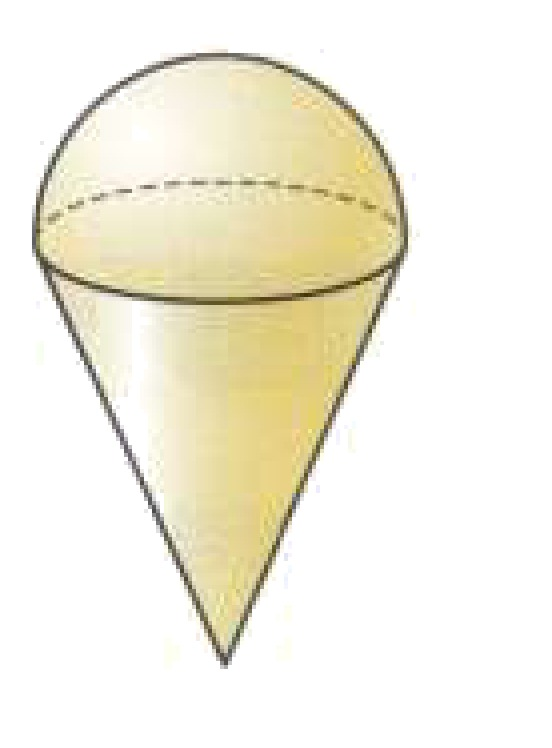
\includegraphics[width=0.92\linewidth]{figures/fig-73-85.jpg}\end{minipage}\par
\noindent \exprbox{\begin{minipage}{0.96\linewidth}\raggedright ㈎ 원뿔의 밑면의 반지름의 길이와 반구의 반지름의 길이가 같다.\par\smallskip ㈏ 원뿔의 밑면의 반지름의 길이와 높이의 합이 $6$으로 일정하다.\end{minipage}}
\dmchoicesauto{\rule[-3ex]{0pt}{8ex}}{$50\pi$}{$\dfrac{160}{3}\pi$}{$\dfrac{170}{3}\pi$}{$60\pi$}{$\dfrac{190}{3}\pi$}
}\vspace{8mm}
\setcounter{dmproblemcount}{85}\dmpnum{73-86}{% id: 73-86
% book: 쎈B 미적분1 · 05 도함수의 활용 (2)
% section: 유형 21 최대·최소의 활용; 부피
% figure: crop:fig-73-86.jpg
% answer: 
% answer_source: 
% variant_level: 0 (원본 전사)
% 이 파일은 build.mjs 가 items.json 에서 만든다. 고칠 때는 items.json 을 고친다.
\smash{\raisebox{1.5mm}{\dmkichul{쎈B 미적분1 73쪽 86번}}}
\noindent\begin{minipage}[t]{0.58\linewidth}\vspace{0pt}\raggedright 오른쪽 그림과 같이 한 변의 길이가 $12$인 정삼각형 모양의 종이의 세 모퉁이에서 사각형을 잘라 내고, 남은 부분으로 뚜껑이 없는 삼각기둥 모양의 상자를 만들려고 한다. 이때 상자의 부피가 최대가 되는 $x$의 값을 구하시오. \dmcondfill{잘라 낸 부분은 모두 합동인 사각형이다.}{}\end{minipage}\hfill\begin{minipage}[t]{0.4\linewidth}\vspace{0pt}\centering 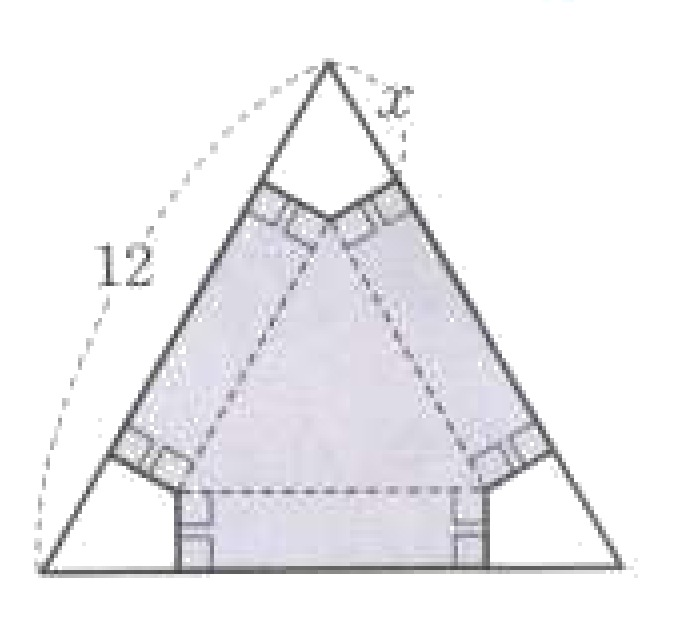
\includegraphics[width=0.92\linewidth]{figures/fig-73-86.jpg}\end{minipage}\par
}\vspace{8mm}
\vspace*{0pt plus 1filll}
\clearpage
\renewcommand{\dmchapunit}{06 도함수의 활용 (3)}
\dmchapter{06}{도함수의 활용 (3)}
\setcounter{dmproblemcount}{0}
\dmsection{유형 01 방정식 $f(x)=k$의 실근의 개수}
\setcounter{dmproblemcount}{0}\dmpnum{75-01}{% id: 75-01
% book: 쎈B 미적분1 · 06 도함수의 활용 (3)
% section: 유형 01 방정식 $f(x)=k$의 실근의 개수
% figure: none
% answer: 
% answer_source: 
% variant_level: 0 (원본 전사)
% 이 파일은 build.mjs 가 items.json 에서 만든다. 고칠 때는 items.json 을 고친다.
\smash{\raisebox{1.5mm}{\dmkichul{쎈B 미적분1 75쪽 01번 · 대표 문제}}}
방정식 $3x^4+4x^3-24x^2-48x-k=0$이 한 중근과 서로 다른 두 개의 실근을 갖도록 하는 모든 실수 $k$의 값의 합은?
\dmchoicesauto{}{$37$}{$38$}{$39$}{$40$}{$41$}
}\vspace{8mm}
\setcounter{dmproblemcount}{1}\dmpnum{75-02}{% id: 75-02
% book: 쎈B 미적분1 · 06 도함수의 활용 (3)
% section: 유형 01 방정식 $f(x)=k$의 실근의 개수
% figure: none
% answer: 
% answer_source: 
% variant_level: 0 (원본 전사)
% 이 파일은 build.mjs 가 items.json 에서 만든다. 고칠 때는 items.json 을 고친다.
\smash{\raisebox{1.5mm}{\dmkichul{쎈B 미적분1 75쪽 02번}}}
방정식 $-x^3+6x^2-k=0$이 $-1\le x\le 5$에서 서로 다른 두 실근을 갖도록 하는 정수 $k$의 개수를 구하시오.
}\vspace{8mm}
\vspace{3mm}\setcounter{dmproblemcount}{2}\dmpnum{75-03}{% id: 75-03
% book: 쎈B 미적분1 · 06 도함수의 활용 (3)
% section: 유형 01 방정식 $f(x)=k$의 실근의 개수
% figure: none
% answer: 
% answer_source: 
% variant_level: 0 (원본 전사)
% 이 파일은 build.mjs 가 items.json 에서 만든다. 고칠 때는 items.json 을 고친다.
\smash{\raisebox{4.5mm}{\dmkichul{쎈B 미적분1 75쪽 03번}}}
방정식 $\dfrac{1}{2}x^4-\dfrac{2}{3}x^3-5x^2-6x+k=0$이 한 중근과 두 허근을 갖도록 하는 실수 $k$의 값은?
\dmchoicesauto{\rule[-3ex]{0pt}{8ex}}{$-\dfrac{81}{2}$}{$-\dfrac{25}{2}$}{$0$}{$\dfrac{25}{2}$}{$\dfrac{81}{2}$}
}\vspace{8mm}
\setcounter{dmproblemcount}{3}\dmpnum{75-04}{% id: 75-04
% book: 쎈B 미적분1 · 06 도함수의 활용 (3)
% section: 유형 01 방정식 $f(x)=k$의 실근의 개수
% figure: none
% answer: 
% answer_source: 
% variant_level: 0 (원본 전사)
% 이 파일은 build.mjs 가 items.json 에서 만든다. 고칠 때는 items.json 을 고친다.
\smash{\raisebox{1.5mm}{\dmkichul{쎈B 미적분1 75쪽 04번 · 서술형}}}
방정식 $3x^4+4x^3-12x^2-k=0$이 서로 다른 두 실근을 갖도록 하는 음의 정수 $k$의 개수를 구하시오.
}\vspace{8mm}
\setcounter{dmproblemcount}{4}\dmpnum{75-05}{% id: 75-05
% book: 쎈B 미적분1 · 06 도함수의 활용 (3)
% section: 유형 01 방정식 $f(x)=k$의 실근의 개수
% figure: tikz:fig-75-05
% answer: 
% answer_source: 
% variant_level: 0 (원본 전사)
% 이 파일은 build.mjs 가 items.json 에서 만든다. 고칠 때는 items.json 을 고친다.
\smash{\raisebox{1.5mm}{\dmkichul{쎈B 미적분1 75쪽 05번}}}
\noindent\begin{minipage}[t]{0.58\linewidth}\vspace{0pt}\raggedright 사차함수 $f(x)$의 도함수 $y=f'(x)$의 그래프가 오른쪽 그림과 같을 때, 사차방정식 $f(x)=0$이 서로 다른 네 실근을 갖기 위한 조건은? \dmcondfill{$\alpha<\beta<\gamma$}{}\end{minipage}\hfill\begin{minipage}[t]{0.4\linewidth}\vspace{0pt}\centering \resizebox{\ifdim\width>\linewidth\linewidth\else\width\fi}{!}{% 75-05(75쪽) — 사차함수 f(x)의 도함수 y=f'(x)(삼차·최고차항 음수)의 그래프. 스캔 화질이 낮아 TikZ 로 다시 그림.
% 원문에 있는 것만: x축 위 문자 α, β, γ(β 는 원점 왼쪽·γ 는 원점 오른쪽) · 라벨 O, x, y, y=f'(x).
% 눈금 숫자·극값 수치는 원문에 없으므로 넣지 않는다(f(α), f(β), f(γ) 의 부호를 고르는 문항이라 수치를 더하면 답이 드러난다).
% 곡선은 원문 모양 그대로 지나는 점들을 재서 smooth 로 잇는다(식이 주어진 그래프가 아니다).
\begin{tikzpicture}[x=0.45cm, y=0.45cm, line width=0.5pt]
  \draw[->, >=stealth, line width=0.7pt] (-4.10,0) -- (2.55,0) node[below=1pt] {$x$};
  \draw[->, >=stealth, line width=0.7pt] (0,-2.40) -- (0,2.25) node[left=1pt] {$y$};
  \draw[line width=0.6pt, smooth] plot coordinates
    {(-3.70,1.78) (-3.45,1.05) (-3.06,0) (-2.80,-0.55) (-2.45,-1.12) (-2.10,-1.45)
     (-1.76,-1.57) (-1.45,-1.50) (-1.15,-1.22) (-0.85,-0.70) (-0.56,0) (-0.30,0.58)
     (0.00,1.00) (0.25,1.17) (0.47,1.20) (0.72,1.10) (0.95,0.85) (1.18,0.48)
     (1.40,0) (1.62,-0.55) (1.85,-1.20) (2.07,-1.92)};
  \node[below=2pt, font=\small] at (-3.24,0) {$\alpha$};
  \node[below=2pt, font=\small] at (-0.46,0) {$\beta$};
  \node[below=2pt, font=\small] at (0.45,0) {$\pt{O}$};
  \node[below=2pt, font=\small] at (1.26,0) {$\gamma$};
  \node[anchor=west, font=\small] at (0.52,1.74) {$y=f'(x)$};
\end{tikzpicture}
}\end{minipage}\par
\begin{choicesv}{$f(\alpha)>0$, $f(\beta)>0$, $f(\gamma)>0$}{$f(\alpha)>0$, $f(\beta)<0$, $f(\gamma)>0$}{$f(\alpha)>0$, $f(\beta)<0$, $f(\gamma)<0$}{$f(\alpha)<0$, $f(\beta)>0$, $f(\gamma)<0$}{$f(\alpha)<0$, $f(\beta)<0$, $f(\gamma)<0$}\end{choicesv}
}\vspace{8mm}
\setcounter{dmproblemcount}{5}\dmpnum{75-06}{% id: 75-06
% book: 쎈B 미적분1 · 06 도함수의 활용 (3)
% section: 유형 01 방정식 $f(x)=k$의 실근의 개수
% figure: none
% answer: 
% answer_source: 
% variant_level: 0 (원본 전사)
% 이 파일은 build.mjs 가 items.json 에서 만든다. 고칠 때는 items.json 을 고친다.
\smash{\raisebox{1.5mm}{\dmkichul{쎈B 미적분1 75쪽 06번}}}
함수 $f(x)=-2x^3+12x^2-18x+5$에 대하여 방정식 $|f(x)|=k$ ($k$는 자연수)의 서로 다른 실근의 개수를 $a_k$라 할 때, $a_1+a_2+a_3+a_4+a_5$의 값은?
\dmchoicesauto{}{$22$}{$23$}{$24$}{$25$}{$26$}
}\vspace{8mm}
\setcounter{dmproblemcount}{6}\dmpnum{76-07}{% id: 76-07
% book: 쎈B 미적분1 · 06 도함수의 활용 (3)
% section: 유형 01 방정식 $f(x)=k$의 실근의 개수
% figure: none
% answer: 
% answer_source: 
% variant_level: 0 (원본 전사)
% 이 파일은 build.mjs 가 items.json 에서 만든다. 고칠 때는 items.json 을 고친다.
\smash{\raisebox{1.5mm}{\dmkichul{쎈B 미적분1 76쪽 07번 · 서술형}}}
최고차항의 계수가 1인 사차함수 $f(x)$가 다음 조건을 모두 만족시킬 때, $f(1)$의 값을 구하시오. \exprbox{\begin{minipage}{0.96\linewidth}\raggedright ㈎ $f(0)=4$\par\smallskip ㈏ 모든 실수 $x$에 대하여 $f(-x)=f(x)$이다.\par\smallskip ㈐ 방정식 $|f(x)|=2$는 서로 다른 6개의 실근을 갖는다.\end{minipage}}
}\vspace{8mm}
\dmsection{유형 02 방정식 $f(x)=k$의 실근의 부호}
\setcounter{dmproblemcount}{7}\dmpnum{76-08}{% id: 76-08
% book: 쎈B 미적분1 · 06 도함수의 활용 (3)
% section: 유형 02 방정식 $f(x)=k$의 실근의 부호
% figure: none
% answer: 
% answer_source: 
% variant_level: 0 (원본 전사)
% 이 파일은 build.mjs 가 items.json 에서 만든다. 고칠 때는 items.json 을 고친다.
\smash{\raisebox{1.5mm}{\dmkichul{쎈B 미적분1 76쪽 08번 · 대표 문제}}}
방정식 $x^3-3x^2-9x+p=0$이 서로 다른 두 개의 양근과 한 개의 음근을 갖도록 하는 실수 $p$의 값의 범위는?
\begin{choicesii}{$-27<p<0$}{$-27<p<5$}{$-5<p<0$}{$-5<p<5$}{$0<p<27$}\end{choicesii}
}\vspace{8mm}
\setcounter{dmproblemcount}{8}\dmpnum{76-09}{% id: 76-09
% book: 쎈B 미적분1 · 06 도함수의 활용 (3)
% section: 유형 02 방정식 $f(x)=k$의 실근의 부호
% figure: none
% answer: 
% answer_source: 
% variant_level: 0 (원본 전사)
% 이 파일은 build.mjs 가 items.json 에서 만든다. 고칠 때는 items.json 을 고친다.
\smash{\raisebox{1.5mm}{\dmkichul{쎈B 미적분1 76쪽 09번}}}
방정식 $-x^3+x^2+8x=x^2-4x+a$가 한 개의 양근과 서로 다른 두 개의 음근을 갖도록 하는 정수 $a$의 개수를 구하시오.
}\vspace{8mm}
\setcounter{dmproblemcount}{9}\dmpnum{76-10}{% id: 76-10
% book: 쎈B 미적분1 · 06 도함수의 활용 (3)
% section: 유형 02 방정식 $f(x)=k$의 실근의 부호
% figure: none
% answer: 
% answer_source: 
% variant_level: 0 (원본 전사)
% 이 파일은 build.mjs 가 items.json 에서 만든다. 고칠 때는 items.json 을 고친다.
\smash{\raisebox{1.5mm}{\dmkichul{쎈B 미적분1 76쪽 10번 · 서술형}}}
방정식 $x^3-9x^2+15x-k=0$이 한 개의 음근과 두 개의 허근을 갖도록 하는 정수 $k$의 최댓값을 구하시오.
}\vspace{8mm}
\vspace{3mm}\setcounter{dmproblemcount}{10}\dmpnum{76-11}{% id: 76-11
% book: 쎈B 미적분1 · 06 도함수의 활용 (3)
% section: 유형 02 방정식 $f(x)=k$의 실근의 부호
% figure: tikz:fig-76-11
% answer: 
% answer_source: 
% variant_level: 0 (원본 전사)
% 이 파일은 build.mjs 가 items.json 에서 만든다. 고칠 때는 items.json 을 고친다.
\smash{\raisebox{4.5mm}{\dmkichul{쎈B 미적분1 76쪽 11번}}}
\noindent\begin{minipage}[t]{0.58\linewidth}\vspace{0pt}\raggedright 삼차함수 $f(x)$의 도함수 $y=f'(x)$의 그래프가 오른쪽 그림과 같고 $f(-3)=\dfrac{21}{2}$, $f(0)=-3$이다. 이때 방정식 $f(x)=k$가 한 개의 양근과 서로 다른 두 개의 음근을 갖도록 하는 실수 $k$의 값의 범위를 구하시오.\end{minipage}\hfill\begin{minipage}[t]{0.4\linewidth}\vspace{0pt}\centering \resizebox{\ifdim\width>\linewidth\linewidth\else\width\fi}{!}{% 76-11(76쪽) — 삼차함수 f(x)의 도함수 y=f'(x)(아래로 볼록한 이차함수)의 그래프. 스캔 화질이 낮아 TikZ 로 다시 그림.
% 원문에 있는 것만: x축 위 눈금 숫자 -3 과 2(f'(x)=0 의 두 근) · 라벨 O, x, y, y=f'(x).
% y축 눈금·꼭짓점 값은 원문에 없으므로 넣지 않는다(k 의 값의 범위가 답이라 수치를 더하면 답이 드러난다).
\begin{tikzpicture}[x=0.28cm, y=0.28cm, line width=0.5pt]
  \draw[->, >=stealth, line width=0.7pt] (-6.0,0) -- (5.9,0) node[below=1pt] {$x$};
  \draw[->, >=stealth, line width=0.7pt] (0,-4.2) -- (0,7.6) node[left=1pt] {$y$};
  \draw[line width=0.6pt, domain=-4.9:4.1, samples=140, smooth] plot (\x, {0.4*(\x+3)*(\x-2)});
  \node[below=2pt, font=\small] at (-3.45,0) {$-3$};
  \node[below=2pt, font=\small] at (2.45,0) {$2$};
  \node[below left=1pt and -2pt, font=\small] at (0,0) {$\pt{O}$};
  \node[anchor=west, font=\small] at (1.0,7.0) {$y=f'(x)$};
\end{tikzpicture}
}\end{minipage}\par
}\vspace{8mm}
\vspace{3mm}\setcounter{dmproblemcount}{11}\dmpnum{76-12}{% id: 76-12
% book: 쎈B 미적분1 · 06 도함수의 활용 (3)
% section: 유형 02 방정식 $f(x)=k$의 실근의 부호
% figure: none
% answer: 
% answer_source: 
% variant_level: 0 (원본 전사)
% 이 파일은 build.mjs 가 items.json 에서 만든다. 고칠 때는 items.json 을 고친다.
\smash{\raisebox{4.5mm}{\dmkichul{쎈B 미적분1 76쪽 12번 · 서술형}}}
자연수 $k$에 대하여 방정식 $\dfrac{1}{4}x^4+x^3+8-k=0$의 음근의 개수를 $f(k)$라 할 때, $\displaystyle\sum_{k=1}^{15} f(k)$의 값을 구하시오.
}\vspace{8mm}
\setcounter{dmproblemcount}{12}\dmpnum{77-13}{% id: 77-13
% book: 쎈B 미적분1 · 06 도함수의 활용 (3)
% section: 유형 02 방정식 $f(x)=k$의 실근의 부호
% figure: none
% answer: 
% answer_source: 
% variant_level: 0 (원본 전사)
% 이 파일은 build.mjs 가 items.json 에서 만든다. 고칠 때는 items.json 을 고친다.
\smash{\raisebox{1.5mm}{\dmkichul{쎈B 미적분1 77쪽 13번}}}
방정식 $2x^4-4x^3-9x^2+7=-x^4+3x^2+k$가 서로 다른 두 개의 양근과 서로 다른 두 개의 음근을 갖도록 하는 실수 $k$의 값의 범위가 $a<k<b$일 때, $ab$의 값은?
\dmchoicesauto{}{$12$}{$14$}{$16$}{$18$}{$20$}
}\vspace{8mm}
\dmsection{유형 03 삼차방정식의 근의 판별}
\vspace{3mm}\setcounter{dmproblemcount}{13}\dmpnum{77-14}{% id: 77-14
% book: 쎈B 미적분1 · 06 도함수의 활용 (3)
% section: 유형 03 삼차방정식의 근의 판별
% figure: none
% answer: 
% answer_source: 
% variant_level: 0 (원본 전사)
% 이 파일은 build.mjs 가 items.json 에서 만든다. 고칠 때는 items.json 을 고친다.
\smash{\raisebox{4.5mm}{\dmkichul{쎈B 미적분1 77쪽 14번 · 대표 문제}}}
방정식 $x^3+\dfrac{3}{2}x^2-18x+n=0$이 서로 다른 세 실근을 갖도록 하는 정수 $n$의 최댓값을 $M$, 최솟값을 $m$이라 할 때, $M-m$의 값은?
\dmchoicesauto{}{$58$}{$59$}{$60$}{$61$}{$62$}
}\vspace{8mm}
\setcounter{dmproblemcount}{14}\dmpnum{77-15}{% id: 77-15
% book: 쎈B 미적분1 · 06 도함수의 활용 (3)
% section: 유형 03 삼차방정식의 근의 판별
% figure: none
% answer: 
% answer_source: 
% variant_level: 0 (원본 전사)
% 이 파일은 build.mjs 가 items.json 에서 만든다. 고칠 때는 items.json 을 고친다.
\smash{\raisebox{1.5mm}{\dmkichul{쎈B 미적분1 77쪽 15번}}}
방정식 $2x^3+3x^2-12x+k=0$이 서로 다른 두 실근을 갖도록 하는 모든 실수 $k$의 값의 합을 구하시오.
}\vspace{8mm}
\setcounter{dmproblemcount}{15}\dmpnum{77-16}{% id: 77-16
% book: 쎈B 미적분1 · 06 도함수의 활용 (3)
% section: 유형 03 삼차방정식의 근의 판별
% figure: none
% answer: 
% answer_source: 
% variant_level: 0 (원본 전사)
% 이 파일은 build.mjs 가 items.json 에서 만든다. 고칠 때는 items.json 을 고친다.
\smash{\raisebox{1.5mm}{\dmkichul{쎈B 미적분1 77쪽 16번}}}
방정식 $x^3+3x^2-9x-a-7=0$이 한 실근과 두 허근을 가질 때, 다음 중 실수 $a$의 값이 될 수 있는 것은?
\dmchoicesauto{}{$-14$}{$-8$}{$2$}{$10$}{$16$}
}\vspace{8mm}
\setcounter{dmproblemcount}{16}\dmpnum{77-17}{% id: 77-17
% book: 쎈B 미적분1 · 06 도함수의 활용 (3)
% section: 유형 03 삼차방정식의 근의 판별
% figure: none
% answer: 
% answer_source: 
% variant_level: 0 (원본 전사)
% 이 파일은 build.mjs 가 items.json 에서 만든다. 고칠 때는 items.json 을 고친다.
\smash{\raisebox{1.5mm}{\dmkichul{쎈B 미적분1 77쪽 17번 · 서술형}}}
함수 $f(x)=2x^3-3(1+n)x^2+6nx$에 대하여 방정식 $f(x)=0$이 서로 다른 세 실근을 갖도록 하는 자연수 $n$의 최솟값을 $a$라 하고, $n=a$일 때 $f(x)$의 극솟값을 $b$라 하자. 이때 $a+b$의 값을 구하시오.
}\vspace{8mm}
\setcounter{dmproblemcount}{17}\dmpnum{77-18}{% id: 77-18
% book: 쎈B 미적분1 · 06 도함수의 활용 (3)
% section: 유형 03 삼차방정식의 근의 판별
% figure: none
% answer: 
% answer_source: 
% variant_level: 0 (원본 전사)
% 이 파일은 build.mjs 가 items.json 에서 만든다. 고칠 때는 items.json 을 고친다.
\smash{\raisebox{1.5mm}{\dmkichul{쎈B 미적분1 77쪽 18번}}}
함수 $f(x)=x^3-3ax+2$가 극값을 가질 때, 방정식 $f(x)=0$이 오직 한 개의 실근을 갖도록 하는 실수 $a$의 값의 범위는?
\begin{choicesii}{$-2<a<-1$}{$-1<a<0$}{$0<a<1$}{$1<a<2$}{$2<a<3$}\end{choicesii}
}\vspace{8mm}
\dmsection{유형 04 두 그래프의 교점의 개수}
\setcounter{dmproblemcount}{18}\dmpnum{78-19}{% id: 78-19
% book: 쎈B 미적분1 · 06 도함수의 활용 (3)
% section: 유형 04 두 그래프의 교점의 개수
% figure: none
% answer: 
% answer_source: 
% variant_level: 0 (원본 전사)
% 이 파일은 build.mjs 가 items.json 에서 만든다. 고칠 때는 items.json 을 고친다.
\smash{\raisebox{1.5mm}{\dmkichul{쎈B 미적분1 78쪽 19번 · 대표 문제}}}
곡선 $y=x^3+3x^2$과 직선 $y=9x+k$가 서로 다른 세 점에서 만나도록 하는 실수 $k$의 값의 범위가 $a<k<b$일 때, $b-a$의 값을 구하시오.
}\vspace{8mm}
\setcounter{dmproblemcount}{19}\dmpnum{78-20}{% id: 78-20
% book: 쎈B 미적분1 · 06 도함수의 활용 (3)
% section: 유형 04 두 그래프의 교점의 개수
% figure: none
% answer: 
% answer_source: 
% variant_level: 0 (원본 전사)
% 이 파일은 build.mjs 가 items.json 에서 만든다. 고칠 때는 items.json 을 고친다.
\smash{\raisebox{1.5mm}{\dmkichul{쎈B 미적분1 78쪽 20번 · 서술형}}}
두 곡선 $y=4x^3-2x^2+x$, $y=x^2+7x-k$가 서로 다른 두 점에서 만나도록 하는 정수 $k$의 값을 구하시오.
}\vspace{8mm}
\setcounter{dmproblemcount}{20}\dmpnum{78-21}{% id: 78-21
% book: 쎈B 미적분1 · 06 도함수의 활용 (3)
% section: 유형 04 두 그래프의 교점의 개수
% figure: none
% answer: 
% answer_source: 
% variant_level: 0 (원본 전사)
% 이 파일은 build.mjs 가 items.json 에서 만든다. 고칠 때는 items.json 을 고친다.
\smash{\raisebox{1.5mm}{\dmkichul{쎈B 미적분1 78쪽 21번}}}
두 곡선 $y=2x^2+3x$, $y=-x^3-x^2+3x-k$가 오직 한 점에서 만나도록 하는 실수 $k$의 값의 범위는?
\begin{choicesii}{$k<-4$ 또는 $k>0$}{$-4<k<0$}{$-4<k<4$}{$-2<k<2$}{$k<0$ 또는 $k>4$}\end{choicesii}
}\vspace{8mm}
\vspace{3mm}\setcounter{dmproblemcount}{21}\dmpnum{78-22}{% id: 78-22
% book: 쎈B 미적분1 · 06 도함수의 활용 (3)
% section: 유형 04 두 그래프의 교점의 개수
% figure: none
% answer: 
% answer_source: 
% variant_level: 0 (원본 전사)
% 이 파일은 build.mjs 가 items.json 에서 만든다. 고칠 때는 items.json 을 고친다.
\smash{\raisebox{4.5mm}{\dmkichul{쎈B 미적분1 78쪽 22번}}}
곡선 $y=\dfrac{2}{3}x^3-3x^2+x+2$와 직선 $y=-3x+k$가 한 점에서 만나고 다른 한 점에서는 접하도록 하는 모든 실수 $k$의 값의 합을 구하시오.
}\vspace{8mm}
\dmsection{유형 05 접선의 개수}
\setcounter{dmproblemcount}{22}\dmpnum{78-23}{% id: 78-23
% book: 쎈B 미적분1 · 06 도함수의 활용 (3)
% section: 유형 05 접선의 개수
% figure: none
% answer: 
% answer_source: 
% variant_level: 0 (원본 전사)
% 이 파일은 build.mjs 가 items.json 에서 만든다. 고칠 때는 items.json 을 고친다.
\smash{\raisebox{1.5mm}{\dmkichul{쎈B 미적분1 78쪽 23번 · 대표 문제}}}
곡선 $y=x^3+k$ 밖의 점 $(2{,}\mkern3mu\mathopen{}5)$에서 주어진 곡선에 서로 다른 두 개의 접선을 그을 수 있도록 하는 실수 $k$의 값은? \dmcondfill{$k\ne-3$}{}
\dmchoicesauto{}{$2$}{$3$}{$4$}{$5$}{$6$}
}\vspace{8mm}
\setcounter{dmproblemcount}{23}\dmpnum{78-24}{% id: 78-24
% book: 쎈B 미적분1 · 06 도함수의 활용 (3)
% section: 유형 05 접선의 개수
% figure: none
% answer: 
% answer_source: 
% variant_level: 0 (원본 전사)
% 이 파일은 build.mjs 가 items.json 에서 만든다. 고칠 때는 items.json 을 고친다.
\smash{\raisebox{1.5mm}{\dmkichul{쎈B 미적분1 78쪽 24번 · 서술형}}}
점 $(1{,}\mkern3mu\mathopen{}a)$에서 곡선 $y=x^3-3x$에 서로 다른 세 개의 접선을 그을 수 있도록 하는 실수 $a$의 값의 범위를 구하시오.
}\vspace{8mm}
\vspace{3mm}\setcounter{dmproblemcount}{24}\dmpnum{78-25}{% id: 78-25
% book: 쎈B 미적분1 · 06 도함수의 활용 (3)
% section: 유형 05 접선의 개수
% figure: none
% answer: 
% answer_source: 
% variant_level: 0 (원본 전사)
% 이 파일은 build.mjs 가 items.json 에서 만든다. 고칠 때는 items.json 을 고친다.
\smash{\raisebox{4.5mm}{\dmkichul{쎈B 미적분1 78쪽 25번}}}
실수 $k$에 대하여 점 $(0{,}\mkern3mu\mathopen{}k)$에서 곡선 $y=x^3-6x^2+2$에 그을 수 있는 접선의 개수를 $n(k)$라 할 때, $\displaystyle\sum_{k=1}^{10} n(k)$의 값은?
\dmchoicesauto{}{$18$}{$20$}{$22$}{$24$}{$26$}
}\vspace{8mm}
\dmsection{유형 06 모든 실수에서 부등식이 항상 성립할 조건}
\vspace{3mm}\setcounter{dmproblemcount}{25}\dmpnum{79-26}{% id: 79-26
% book: 쎈B 미적분1 · 06 도함수의 활용 (3)
% section: 유형 06 모든 실수에서 부등식이 항상 성립할 조건
% figure: none
% answer: 
% answer_source: 
% variant_level: 0 (원본 전사)
% 이 파일은 build.mjs 가 items.json 에서 만든다. 고칠 때는 items.json 을 고친다.
\smash{\raisebox{4.5mm}{\dmkichul{쎈B 미적분1 79쪽 26번 · 대표 문제}}}
모든 실수 $x$에 대하여 부등식 $\dfrac{3}{2}x^4-9x^2+12x+k\ge 0$이 성립하도록 하는 실수 $k$의 최솟값은?
\dmchoicesauto{\rule[-3ex]{0pt}{8ex}}{$-18$}{$-\dfrac{9}{2}$}{$\dfrac{9}{2}$}{$18$}{$36$}
}\vspace{8mm}
\setcounter{dmproblemcount}{26}\dmpnum{79-27}{% id: 79-27
% book: 쎈B 미적분1 · 06 도함수의 활용 (3)
% section: 유형 06 모든 실수에서 부등식이 항상 성립할 조건
% figure: none
% answer: 
% answer_source: 
% variant_level: 0 (원본 전사)
% 이 파일은 build.mjs 가 items.json 에서 만든다. 고칠 때는 items.json 을 고친다.
\smash{\raisebox{1.5mm}{\dmkichul{쎈B 미적분1 79쪽 27번}}}
모든 실수 $x$에 대하여 부등식 $-x^4+6x^2+8x<k$가 성립하도록 하는 정수 $k$의 최솟값은?
\dmchoicesauto{}{$21$}{$22$}{$23$}{$24$}{$25$}
}\vspace{8mm}
\setcounter{dmproblemcount}{27}\dmpnum{79-28}{% id: 79-28
% book: 쎈B 미적분1 · 06 도함수의 활용 (3)
% section: 유형 06 모든 실수에서 부등식이 항상 성립할 조건
% figure: none
% answer: 
% answer_source: 
% variant_level: 0 (원본 전사)
% 이 파일은 build.mjs 가 items.json 에서 만든다. 고칠 때는 items.json 을 고친다.
\smash{\raisebox{1.5mm}{\dmkichul{쎈B 미적분1 79쪽 28번 · 서술형}}}
모든 실수 $x$에 대하여 부등식 $x^4+2ax^2-4(a+1)x+a^2-5\ge 0$이 성립하도록 하는 양수 $a$의 값의 범위를 구하시오.
}\vspace{8mm}
\setcounter{dmproblemcount}{28}\dmpnum{79-29}{% id: 79-29
% book: 쎈B 미적분1 · 06 도함수의 활용 (3)
% section: 유형 06 모든 실수에서 부등식이 항상 성립할 조건
% figure: none
% answer: 
% answer_source: 
% variant_level: 0 (원본 전사)
% 이 파일은 build.mjs 가 items.json 에서 만든다. 고칠 때는 items.json 을 고친다.
\smash{\raisebox{1.5mm}{\dmkichul{쎈B 미적분1 79쪽 29번}}}
모든 실수 $x$에 대하여 부등식 $x^4-4k^3x+12>0$이 성립하도록 하는 정수 $k$의 개수를 구하시오.
}\vspace{8mm}
\dmsection{유형 07 주어진 구간에서 부등식이 항상 성립할 조건; 증가·감소의 활용}
\setcounter{dmproblemcount}{29}\dmpnum{79-30}{% id: 79-30
% book: 쎈B 미적분1 · 06 도함수의 활용 (3)
% section: 유형 07 주어진 구간에서 부등식이 항상 성립할 조건; 증가·감소의 활용
% figure: none
% answer: 
% answer_source: 
% variant_level: 0 (원본 전사)
% 이 파일은 build.mjs 가 items.json 에서 만든다. 고칠 때는 items.json 을 고친다.
\smash{\raisebox{1.5mm}{\dmkichul{쎈B 미적분1 79쪽 30번 · 대표 문제}}}
$-1<x<1$일 때, 부등식 $x^3-12x+k>0$이 항상 성립하도록 하는 실수 $k$의 값의 범위는?
\begin{choicesii}{$k\le -11$}{$-11\le k<0$}{$-11\le k\le 11$}{$0<k\le 11$}{$k\ge 11$}\end{choicesii}
}\vspace{8mm}
\setcounter{dmproblemcount}{30}\dmpnum{79-31}{% id: 79-31
% book: 쎈B 미적분1 · 06 도함수의 활용 (3)
% section: 유형 07 주어진 구간에서 부등식이 항상 성립할 조건; 증가·감소의 활용
% figure: none
% answer: 
% answer_source: 
% variant_level: 0 (원본 전사)
% 이 파일은 build.mjs 가 items.json 에서 만든다. 고칠 때는 items.json 을 고친다.
\smash{\raisebox{1.5mm}{\dmkichul{쎈B 미적분1 79쪽 31번 · 서술형}}}
$x>2$일 때, 부등식 $x^3-3x^2+k>0$이 항상 성립하도록 하는 실수 $k$의 최솟값을 구하시오.
}\vspace{8mm}
\vspace{3mm}\setcounter{dmproblemcount}{31}\dmpnum{80-32}{% id: 80-32
% book: 쎈B 미적분1 · 06 도함수의 활용 (3)
% section: 유형 07 주어진 구간에서 부등식이 항상 성립할 조건; 증가·감소의 활용
% figure: none
% answer: 
% answer_source: 
% variant_level: 0 (원본 전사)
% 이 파일은 build.mjs 가 items.json 에서 만든다. 고칠 때는 items.json 을 고친다.
\smash{\raisebox{4.5mm}{\dmkichul{쎈B 미적분1 80쪽 32번}}}
$\dfrac{3}{2}<x<3$일 때, 부등식 $x^3+x^2<-\dfrac{1}{3}x^3+6x-k$가 항상 성립하도록 하는 실수 $k$의 최댓값은?
\dmchoicesauto{}{$-30$}{$-29$}{$-28$}{$-27$}{$-26$}
}\vspace{8mm}
\setcounter{dmproblemcount}{32}\dmpnum{80-33}{% id: 80-33
% book: 쎈B 미적분1 · 06 도함수의 활용 (3)
% section: 유형 07 주어진 구간에서 부등식이 항상 성립할 조건; 증가·감소의 활용
% figure: none
% answer: 
% answer_source: 
% variant_level: 0 (원본 전사)
% 이 파일은 build.mjs 가 items.json 에서 만든다. 고칠 때는 items.json 을 고친다.
\smash{\raisebox{1.5mm}{\dmkichul{쎈B 미적분1 80쪽 33번}}}
$x<1$에서 곡선 $y=x^3+x^2$이 직선 $y=-2x+k$보다 항상 아래쪽에 있도록 하는 실수 $k$의 값의 범위가 $k\ge a$일 때, $a$의 값을 구하시오.
}\vspace{8mm}
\dmsection{유형 08 주어진 구간에서 부등식이 항상 성립할 조건; 최대·최소의 활용}
\vspace{3mm}\setcounter{dmproblemcount}{33}\dmpnum{80-34}{% id: 80-34
% book: 쎈B 미적분1 · 06 도함수의 활용 (3)
% section: 유형 08 주어진 구간에서 부등식이 항상 성립할 조건; 최대·최소의 활용
% figure: none
% answer: 
% answer_source: 
% variant_level: 0 (원본 전사)
% 이 파일은 build.mjs 가 items.json 에서 만든다. 고칠 때는 items.json 을 고친다.
\smash{\raisebox{4.5mm}{\dmkichul{쎈B 미적분1 80쪽 34번 · 대표 문제}}}
$x\le 2$일 때, 부등식 $2x^3-\dfrac{9}{2}x^2+3x\le k$가 항상 성립하도록 하는 실수 $k$의 최솟값은?
\dmchoicesauto{}{$-7$}{$-4$}{$-1$}{$4$}{$7$}
}\vspace{8mm}
\setcounter{dmproblemcount}{34}\dmpnum{80-35}{% id: 80-35
% book: 쎈B 미적분1 · 06 도함수의 활용 (3)
% section: 유형 08 주어진 구간에서 부등식이 항상 성립할 조건; 최대·최소의 활용
% figure: none
% answer: 
% answer_source: 
% variant_level: 0 (원본 전사)
% 이 파일은 build.mjs 가 items.json 에서 만든다. 고칠 때는 items.json 을 고친다.
\smash{\raisebox{1.5mm}{\dmkichul{쎈B 미적분1 80쪽 35번}}}
$x>0$일 때, 부등식 $x^3-4x^2-10x\ge -x^2+14x-k$가 항상 성립하도록 하는 실수 $k$의 값의 범위는?
\dmchoicesauto{}{$k\le -52$}{$k\le -26$}{$k\le 26$}{$k\ge 52$}{$k\ge 80$}
}\vspace{8mm}
\vspace{3mm}\setcounter{dmproblemcount}{35}\dmpnum{80-36}{% id: 80-36
% book: 쎈B 미적분1 · 06 도함수의 활용 (3)
% section: 유형 08 주어진 구간에서 부등식이 항상 성립할 조건; 최대·최소의 활용
% figure: none
% answer: 
% answer_source: 
% variant_level: 0 (원본 전사)
% 이 파일은 build.mjs 가 items.json 에서 만든다. 고칠 때는 items.json 을 고친다.
\smash{\raisebox{4.5mm}{\dmkichul{쎈B 미적분1 80쪽 36번 · 서술형}}}
$-3\le x\le 2$에서 부등식 $-18\le \dfrac{2}{3}x^3-x^2-4x+k\le 2$가 항상 성립하도록 하는 모든 정수 $k$의 값의 합을 구하시오.
}\vspace{8mm}
\setcounter{dmproblemcount}{36}\dmpnum{80-37}{% id: 80-37
% book: 쎈B 미적분1 · 06 도함수의 활용 (3)
% section: 유형 08 주어진 구간에서 부등식이 항상 성립할 조건; 최대·최소의 활용
% figure: none
% answer: 
% answer_source: 
% variant_level: 0 (원본 전사)
% 이 파일은 build.mjs 가 items.json 에서 만든다. 고칠 때는 items.json 을 고친다.
\smash{\raisebox{1.5mm}{\dmkichul{쎈B 미적분1 80쪽 37번}}}
어느 운송 회사가 일정한 무게의 물품을 시내에서 $x\mkern3mu \mathrm{km}$ 떨어진 곳에 배달하는 데 드는 비용은 $(144x+5000)$원이다. 배달 요금으로 $(2x^3+6x^2+a)$원을 받는다고 할 때, 이 회사가 손해를 보지 않도록 하는 상수 $a$의 최솟값을 구하시오.
}\vspace{8mm}
\dmsection{유형 09 부등식 $f(x)>g(x)$가 항상 성립할 조건}
\setcounter{dmproblemcount}{37}\dmpnum{81-38}{% id: 81-38
% book: 쎈B 미적분1 · 06 도함수의 활용 (3)
% section: 유형 09 부등식 $f(x)>g(x)$가 항상 성립할 조건
% figure: none
% answer: 
% answer_source: 
% variant_level: 0 (원본 전사)
% 이 파일은 build.mjs 가 items.json 에서 만든다. 고칠 때는 items.json 을 고친다.
\smash{\raisebox{1.5mm}{\dmkichul{쎈B 미적분1 81쪽 38번 · 대표 문제}}}
두 함수\par\smallskip\dispeq{$f(x)=x^4-3x^3+x^2-2x+a$, $g(x)=x^3-3x^2-2x$}\par\smallskip\noindent 에 대하여 $y=f(x)$의 그래프가 $y=g(x)$의 그래프보다 항상 위쪽에 있을 때, 실수 $a$의 값의 범위는?
\dmchoicesauto{}{$a<-2$}{$a<-1$}{$a<0$}{$a>-1$}{$a>0$}
}\vspace{8mm}
\setcounter{dmproblemcount}{38}\dmpnum{81-39}{% id: 81-39
% book: 쎈B 미적분1 · 06 도함수의 활용 (3)
% section: 유형 09 부등식 $f(x)>g(x)$가 항상 성립할 조건
% figure: none
% answer: 
% answer_source: 
% variant_level: 0 (원본 전사)
% 이 파일은 build.mjs 가 items.json 에서 만든다. 고칠 때는 items.json 을 고친다.
\smash{\raisebox{1.5mm}{\dmkichul{쎈B 미적분1 81쪽 39번}}}
두 함수 $f(x)=x^4-3x^2$, $g(x)=4x^3+3x^2-a$가 있다. 모든 실수 $x$에 대하여 부등식 $3f(x)\ge g(x)$가 성립하도록 하는 실수 $a$의 최솟값을 구하시오.
}\vspace{8mm}
\setcounter{dmproblemcount}{39}\dmpnum{81-40}{% id: 81-40
% book: 쎈B 미적분1 · 06 도함수의 활용 (3)
% section: 유형 09 부등식 $f(x)>g(x)$가 항상 성립할 조건
% figure: none
% answer: 
% answer_source: 
% variant_level: 0 (원본 전사)
% 이 파일은 build.mjs 가 items.json 에서 만든다. 고칠 때는 items.json 을 고친다.
\smash{\raisebox{1.5mm}{\dmkichul{쎈B 미적분1 81쪽 40번}}}
두 함수\par\smallskip\dispeq{$f(x)=-2x^3+x^2$, $g(x)=-5x^2-a$}\par\smallskip\noindent 에 대하여 $-2\le x\le 2$일 때, 부등식 $f(x)\le g(x)$가 항상 성립하도록 하는 실수 $a$의 최댓값을 구하시오.
}\vspace{8mm}
\setcounter{dmproblemcount}{40}\dmpnum{81-41}{% id: 81-41
% book: 쎈B 미적분1 · 06 도함수의 활용 (3)
% section: 유형 09 부등식 $f(x)>g(x)$가 항상 성립할 조건
% figure: none
% answer: 
% answer_source: 
% variant_level: 0 (원본 전사)
% 이 파일은 build.mjs 가 items.json 에서 만든다. 고칠 때는 items.json 을 고친다.
\smash{\raisebox{1.5mm}{\dmkichul{쎈B 미적분1 81쪽 41번 · 서술형}}}
두 함수\par\smallskip\dispeq{$f(x)=-x^3+3x-2$, $g(x)=k(x+2)$}\par\smallskip\noindent 에 대하여 $x\ge -2$일 때, 부등식 $f(x)\le g(x)$가 항상 성립하도록 하는 실수 $k$의 값의 범위를 구하시오.
}\vspace{8mm}
\vspace{3mm}\setcounter{dmproblemcount}{41}\dmpnum{81-42}{% id: 81-42
% book: 쎈B 미적분1 · 06 도함수의 활용 (3)
% section: 유형 09 부등식 $f(x)>g(x)$가 항상 성립할 조건
% figure: none
% answer: 
% answer_source: 
% variant_level: 0 (원본 전사)
% 이 파일은 build.mjs 가 items.json 에서 만든다. 고칠 때는 items.json 을 고친다.
\smash{\raisebox{4.5mm}{\dmkichul{쎈B 미적분1 81쪽 42번}}}
자연수 $n$에 대하여 두 함수 $f(x)$, $g(x)$를\par\smallskip\dispeq{$f(x)=-\dfrac{1}{2}x^4+2x^2-12x$, $g(x)=4x^2+n$}\par\smallskip\noindent 이라 하자. 모든 실수 $x$에 대하여 부등식 $f(x)\le -4x+k\le g(x)$를 만족시키는 정수 $k$의 개수가 $3$일 때, $n$의 값을 구하시오.
}\vspace{8mm}
\dmsection{유형 10 속도}
\setcounter{dmproblemcount}{42}\dmpnum{81-43}{% id: 81-43
% book: 쎈B 미적분1 · 06 도함수의 활용 (3)
% section: 유형 10 속도
% figure: none
% answer: 
% answer_source: 
% variant_level: 0 (원본 전사)
% 이 파일은 build.mjs 가 items.json 에서 만든다. 고칠 때는 items.json 을 고친다.
\smash{\raisebox{1.5mm}{\dmkichul{쎈B 미적분1 81쪽 43번 · 대표 문제}}}
원점을 출발하여 수직선 위를 움직이는 점~$\pt{P}$의 시각 $t$에서의 위치가 $x=t^3-2t^2+t$일 때, 점~$\pt{P}$가 출발 후 다시 원점을 지나는 순간의 속도를 구하시오.
}\vspace{8mm}
\setcounter{dmproblemcount}{43}\dmpnum{82-44}{% id: 82-44
% book: 쎈B 미적분1 · 06 도함수의 활용 (3)
% section: 유형 10 속도
% figure: none
% answer: 
% answer_source: 
% variant_level: 0 (원본 전사)
% 이 파일은 build.mjs 가 items.json 에서 만든다. 고칠 때는 items.json 을 고친다.
\smash{\raisebox{1.5mm}{\dmkichul{쎈B 미적분1 82쪽 44번}}}
원점을 출발하여 수직선 위를 움직이는 점~$\pt{P}$의 시각 $t$에서의 위치가 $x=t^3-2at^2+4t$이고 $t=4$에서의 점~$\pt{P}$의 속도가 $20$이다. 이때 상수 $a$의 값은?
\dmchoicesauto{}{$-3$}{$-2$}{$0$}{$2$}{$3$}
}\vspace{8mm}
\vspace{3mm}\setcounter{dmproblemcount}{44}\dmpnum{82-45}{% id: 82-45
% book: 쎈B 미적분1 · 06 도함수의 활용 (3)
% section: 유형 10 속도
% figure: none
% answer: 
% answer_source: 
% variant_level: 0 (원본 전사)
% 이 파일은 build.mjs 가 items.json 에서 만든다. 고칠 때는 items.json 을 고친다.
\smash{\raisebox{4.5mm}{\dmkichul{쎈B 미적분1 82쪽 45번 · 서술형}}}
수직선 위를 움직이는 두 점~$\pt{P}$, $\pt{Q}$의 시각 $t$에서의 위치가 각각\par\smallskip\dispeq{$x_{\pt{P}}=\dfrac{2}{3}t^3+2t^2+\dfrac{2}{3}$, $x_{\pt{Q}}=3t^2+4t$}\par\smallskip\noindent 이다. 두 점~$\pt{P}$, $\pt{Q}$의 속도가 같아지는 순간에서의 두 점 사이의 거리를 구하시오.
}\vspace{8mm}
\vspace{3mm}\setcounter{dmproblemcount}{45}\dmpnum{82-46}{% id: 82-46
% book: 쎈B 미적분1 · 06 도함수의 활용 (3)
% section: 유형 10 속도
% figure: none
% answer: 
% answer_source: 
% variant_level: 0 (원본 전사)
% 이 파일은 build.mjs 가 items.json 에서 만든다. 고칠 때는 items.json 을 고친다.
\smash{\raisebox{4.5mm}{\dmkichul{쎈B 미적분1 82쪽 46번}}}
원점을 출발하여 수직선 위를 움직이는 점~$\pt{P}$의 시각 $t$에서의 위치가 $f(t)=\dfrac{1}{3}t^3-2t^2-5t$일 때, $1\le t\le 6$에서 점~$\pt{P}$의 속력의 최댓값을 $M$, 그때의 시각을 $a$라 하자. 이때 $M+a$의 값은?
\dmchoicesauto{}{$8$}{$9$}{$10$}{$11$}{$12$}
}\vspace{8mm}
\setcounter{dmproblemcount}{46}\dmpnum{82-47}{% id: 82-47
% book: 쎈B 미적분1 · 06 도함수의 활용 (3)
% section: 유형 10 속도
% figure: none
% answer: 
% answer_source: 
% variant_level: 0 (원본 전사)
% 이 파일은 build.mjs 가 items.json 에서 만든다. 고칠 때는 items.json 을 고친다.
\smash{\raisebox{1.5mm}{\dmkichul{쎈B 미적분1 82쪽 47번 · 서술형}}}
수직선 위를 움직이는 두 점~$\pt{P}$, $\pt{Q}$의 시각 $t$에서의 위치를 각각 $f(t)$, $g(t)$라 하면\par\smallskip\dispeq{$f(t)-g(t)=t^3+at^2+24t+b$}\par\smallskip\noindent 이다. $t=2$에서 두 점~$\pt{P}$, $\pt{Q}$가 처음으로 만나고, 그때의 속도가 같았을 때, 속도가 다시 같아지는 시각에서의 두 점 사이의 거리를 구하시오. \dmcondfill{$a$, $b$는 상수이다.}{}
}\vspace{8mm}
\dmsection{유형 11 가속도}
\vspace{3mm}\setcounter{dmproblemcount}{47}\dmpnum{82-48}{% id: 82-48
% book: 쎈B 미적분1 · 06 도함수의 활용 (3)
% section: 유형 11 가속도
% figure: none
% answer: 
% answer_source: 
% variant_level: 0 (원본 전사)
% 이 파일은 build.mjs 가 items.json 에서 만든다. 고칠 때는 items.json 을 고친다.
\smash{\raisebox{4.5mm}{\dmkichul{쎈B 미적분1 82쪽 48번 · 대표 문제}}}
원점을 출발하여 수직선 위를 움직이는 점~$\pt{P}$의 시각 $t$에서의 위치가 $x=t^3-\dfrac{3}{2}t^2-12t$이다. 속도가 $6$인 순간의 점~$\pt{P}$의 가속도를 구하시오.
}\vspace{8mm}
\setcounter{dmproblemcount}{48}\dmpnum{82-49}{% id: 82-49
% book: 쎈B 미적분1 · 06 도함수의 활용 (3)
% section: 유형 11 가속도
% figure: none
% answer: 
% answer_source: 
% variant_level: 0 (원본 전사)
% 이 파일은 build.mjs 가 items.json 에서 만든다. 고칠 때는 items.json 을 고친다.
\smash{\raisebox{1.5mm}{\dmkichul{쎈B 미적분1 82쪽 49번}}}
수직선 위를 움직이는 점~$\pt{P}$의 시각 $t$에서의 위치가\par\smallskip\dispeq{$x=-t^3+6t^2-10t+k$}\par\smallskip\noindent 이고, 점~$\pt{P}$의 가속도가 $0$인 순간의 점~$\pt{P}$의 위치는 $9$이다. 이때 상수 $k$의 값은?
\dmchoicesauto{}{$11$}{$12$}{$13$}{$14$}{$15$}
}\vspace{8mm}
\vspace{3mm}\setcounter{dmproblemcount}{49}\dmpnum{83-50}{% id: 83-50
% book: 쎈B 미적분1 · 06 도함수의 활용 (3)
% section: 유형 11 가속도
% figure: none
% answer: 
% answer_source: 
% variant_level: 0 (원본 전사)
% 이 파일은 build.mjs 가 items.json 에서 만든다. 고칠 때는 items.json 을 고친다.
\smash{\raisebox{4.5mm}{\dmkichul{쎈B 미적분1 83쪽 50번}}}
수직선 위를 움직이는 점~$\pt{P}$의 시각 $t$에서의 위치가 \par\smallskip\dispeq{$x=\dfrac{1}{2}t^4-t^3+kt^2-8t+5$}\par\smallskip\noindent 이다. $t=2$에서의 점~$\pt{P}$의 속도가 $16$일 때, $t=2$에서의 점~$\pt{P}$의 가속도는? \dmcondfill{$k$는 상수이다.}{}
\dmchoicesauto{}{$5$}{$8$}{$12$}{$18$}{$22$}
}\vspace{8mm}
\dmsection{유형 12 속도·가속도와 운동 방향}
\setcounter{dmproblemcount}{50}\dmpnum{83-51}{% id: 83-51
% book: 쎈B 미적분1 · 06 도함수의 활용 (3)
% section: 유형 12 속도·가속도와 운동 방향
% figure: none
% answer: 
% answer_source: 
% variant_level: 0 (원본 전사)
% 이 파일은 build.mjs 가 items.json 에서 만든다. 고칠 때는 items.json 을 고친다.
\smash{\raisebox{1.5mm}{\dmkichul{쎈B 미적분1 83쪽 51번 · 대표 문제}}}
원점을 출발하여 수직선 위를 움직이는 점~$\pt{P}$의 시각 $t$에서의 위치가 $x=t^3-9t^2+24t$이고, 점~$\pt{P}$는 출발 후 운동 방향을 두 번 바꾼다. 운동 방향을 바꾸는 순간의 위치를 각각 $\pt{A}$, $\pt{B}$라 할 때, 두 점~$\pt{A}$, $\pt{B}$ 사이의 거리를 구하시오.
}\vspace{8mm}
\vspace{3mm}\setcounter{dmproblemcount}{51}\dmpnum{83-52}{% id: 83-52
% book: 쎈B 미적분1 · 06 도함수의 활용 (3)
% section: 유형 12 속도·가속도와 운동 방향
% figure: none
% answer: 
% answer_source: 
% variant_level: 0 (원본 전사)
% 이 파일은 build.mjs 가 items.json 에서 만든다. 고칠 때는 items.json 을 고친다.
\smash{\raisebox{4.5mm}{\dmkichul{쎈B 미적분1 83쪽 52번}}}
원점을 출발하여 수직선 위를 움직이는 점~$\pt{P}$의 시각 $t$에서의 위치가 $x=\dfrac{1}{3}t^3-4t^2+15t$일 때, 점~$\pt{P}$가 출발 후 두 번째로 운동 방향을 바꾸는 순간의 가속도는?
\dmchoicesauto{\rule[-3ex]{0pt}{8ex}}{$\dfrac{2}{3}$}{$2$}{$\dfrac{10}{3}$}{$\dfrac{14}{3}$}{$6$}
}\vspace{8mm}
\vspace{3mm}\setcounter{dmproblemcount}{52}\dmpnum{83-53}{% id: 83-53
% book: 쎈B 미적분1 · 06 도함수의 활용 (3)
% section: 유형 12 속도·가속도와 운동 방향
% figure: none
% answer: 
% answer_source: 
% variant_level: 0 (원본 전사)
% 이 파일은 build.mjs 가 items.json 에서 만든다. 고칠 때는 items.json 을 고친다.
\smash{\raisebox{4.5mm}{\dmkichul{쎈B 미적분1 83쪽 53번}}}
수직선 위를 움직이는 점~$\pt{P}$의 시각 $t$에서의 위치가 \par\smallskip\dispeq{$x=-\dfrac{2}{3}t^3+5t^2-2(a+4)t-3$}\par\smallskip\noindent 일 때, 점~$\pt{P}$의 운동 방향이 바뀌지 않도록 하는 실수 $a$의 최솟값은?
\dmchoicesauto{\rule[-3ex]{0pt}{8ex}}{$-\dfrac{9}{4}$}{$-\dfrac{1}{4}$}{$\dfrac{1}{4}$}{$\dfrac{9}{4}$}{$\dfrac{13}{4}$}
}\vspace{8mm}
\setcounter{dmproblemcount}{53}\dmpnum{83-54}{% id: 83-54
% book: 쎈B 미적분1 · 06 도함수의 활용 (3)
% section: 유형 12 속도·가속도와 운동 방향
% figure: none
% answer: 
% answer_source: 
% variant_level: 0 (원본 전사)
% 이 파일은 build.mjs 가 items.json 에서 만든다. 고칠 때는 items.json 을 고친다.
\smash{\raisebox{1.5mm}{\dmkichul{쎈B 미적분1 83쪽 54번 · 서술형}}}
수직선 위를 움직이는 두 점~$\pt{A}$, $\pt{B}$의 시각 $t$에서의 위치가 각각 \par\smallskip\dispeq{$f(t)=2t^3-7t^2+3t+4,\ g(t)=-t^2+5t+2$}\par\smallskip\noindent 일 때, 선분~$\pt{AB}$의 중점~$\pt{M}$이 운동 방향을 몇 번 바꾸는지 구하시오.
}\vspace{8mm}
\setcounter{dmproblemcount}{54}\dmpnum{83-55}{% id: 83-55
% book: 쎈B 미적분1 · 06 도함수의 활용 (3)
% section: 유형 12 속도·가속도와 운동 방향
% figure: none
% answer: 
% answer_source: 
% variant_level: 0 (원본 전사)
% 이 파일은 build.mjs 가 items.json 에서 만든다. 고칠 때는 items.json 을 고친다.
\smash{\raisebox{1.5mm}{\dmkichul{쎈B 미적분1 83쪽 55번}}}
수직선 위를 움직이는 두 점~$\pt{P}$, $\pt{Q}$의 시각 $t$에서의 위치가 각각 \par\smallskip\dispeq{$x_{\pt{P}}=2t^2-2t+3,\ x_{\pt{Q}}=t^2-10t-5$}\par\smallskip\noindent 일 때, 다음 중 두 점~$\pt{P}$, $\pt{Q}$가 서로 반대 방향으로 움직이는 시각 $t$의 값의 범위는?
\begin{choicesii}{\rule[-3ex]{0pt}{8ex}$0<t<\dfrac{1}{2}$}{\rule[-3ex]{0pt}{8ex}$0<t<5$}{\rule[-3ex]{0pt}{8ex}$\dfrac{1}{2}<t<5$}{\rule[-3ex]{0pt}{8ex}$0<t<\dfrac{1}{2}$ 또는 $t>5$}{\rule[-3ex]{0pt}{8ex}$\dfrac{1}{2}<t<2$ 또는 $t>5$}\end{choicesii}
}\vspace{8mm}
\setcounter{dmproblemcount}{55}\dmpnum{84-56}{% id: 84-56
% book: 쎈B 미적분1 · 06 도함수의 활용 (3)
% section: 유형 12 속도·가속도와 운동 방향
% figure: none
% answer: 
% answer_source: 
% variant_level: 0 (원본 전사)
% 이 파일은 build.mjs 가 items.json 에서 만든다. 고칠 때는 items.json 을 고친다.
\smash{\raisebox{1.5mm}{\dmkichul{쎈B 미적분1 84쪽 56번 · 서술형}}}
수직선 위를 움직이는 점~$\pt{P}$의 시각 $t$에서의 위치가 $x=t^3-mt^2+nt-6$이다. 점~$\pt{P}$는 $t=1$에서 운동 방향을 바꾸고 그때의 위치가 $1$일 때, 점~$\pt{P}$가 $t=1$ 이외에 운동 방향을 바꾸는 순간의 가속도를 구하시오. \dmcondfill{$m$, $n$은 상수이다.}{}
}\vspace{8mm}
\dmsection{유형 13 정지하는 물체의 속도와 움직인 거리}
\setcounter{dmproblemcount}{56}\dmpnum{84-57}{% id: 84-57
% book: 쎈B 미적분1 · 06 도함수의 활용 (3)
% section: 유형 13 정지하는 물체의 속도와 움직인 거리
% figure: none
% answer: 
% answer_source: 
% variant_level: 0 (원본 전사)
% 이 파일은 build.mjs 가 items.json 에서 만든다. 고칠 때는 items.json 을 고친다.
\smash{\raisebox{1.5mm}{\dmkichul{쎈B 미적분1 84쪽 57번 · 대표 문제}}}
직선 궤도를 달리는 열차가 제동을 건 후 $t$초 동안 움직인 거리를 $x\mkern3mu \mathrm{m}$라 하면 $x=32t-0.8t^2$이다. 이 열차가 제동을 건 후 정지할 때까지 움직인 거리를 구하시오.
}\vspace{8mm}
\setcounter{dmproblemcount}{57}\dmpnum{84-58}{% id: 84-58
% book: 쎈B 미적분1 · 06 도함수의 활용 (3)
% section: 유형 13 정지하는 물체의 속도와 움직인 거리
% figure: none
% answer: 
% answer_source: 
% variant_level: 0 (원본 전사)
% 이 파일은 build.mjs 가 items.json 에서 만든다. 고칠 때는 items.json 을 고친다.
\smash{\raisebox{1.5mm}{\dmkichul{쎈B 미적분1 84쪽 58번}}}
어떤 자동차가 브레이크를 밟은 후 $t$초 동안 달린 거리를 $x\mkern3mu \mathrm{m}$라 하면 $x=24t-4t^2$이다. 브레이크를 밟은 후 자동차가 정지할 때까지 걸린 시간은?
\dmchoicesauto{}{$2$초}{$3$초}{$4$초}{$5$초}{$6$초}
}\vspace{8mm}
\setcounter{dmproblemcount}{58}\dmpnum{84-59}{% id: 84-59
% book: 쎈B 미적분1 · 06 도함수의 활용 (3)
% section: 유형 13 정지하는 물체의 속도와 움직인 거리
% figure: none
% answer: 
% answer_source: 
% variant_level: 0 (원본 전사)
% 이 파일은 build.mjs 가 items.json 에서 만든다. 고칠 때는 items.json 을 고친다.
\smash{\raisebox{1.5mm}{\dmkichul{쎈B 미적분1 84쪽 59번 · 서술형}}}
직선 도로를 달리는 자동차가 제동을 건 후 $t$초 동안 움직인 거리를 $x\mkern3mu \mathrm{m}$라 하면 $x=14.4t-0.72t^2$이다. 이 자동차가 목적지에 정확히 정차하려면 목적지로부터 전방 $a\mkern3mu \mathrm{m}$의 지점에서 제동을 걸어야 한다고 할 때, 상수 $a$의 값을 구하시오.
}\vspace{8mm}
\dmsection{유형 14 위로 던진 물체의 위치와 속도}
\setcounter{dmproblemcount}{59}\dmpnum{84-60}{% id: 84-60
% book: 쎈B 미적분1 · 06 도함수의 활용 (3)
% section: 유형 14 위로 던진 물체의 위치와 속도
% figure: none
% answer: 
% answer_source: 
% variant_level: 0 (원본 전사)
% 이 파일은 build.mjs 가 items.json 에서 만든다. 고칠 때는 items.json 을 고친다.
\smash{\raisebox{1.5mm}{\dmkichul{쎈B 미적분1 84쪽 60번 · 대표 문제}}}
지면에서 처음 속도 $50\mkern3mu \mathrm{m/s}$로 지면과 수직하게 위로 쏘아 올린 로켓의 $t$초 후의 높이를 $h\mkern3mu \mathrm{m}$라 하면 $h=50t-5t^2$이다. 이 로켓이 최고 지점에 도달했을 때 지면으로부터의 높이는?
\begin{choices32}{$110\mkern3mu \mathrm{m}$}{$115\mkern3mu \mathrm{m}$}{$120\mkern3mu \mathrm{m}$}{$125\mkern3mu \mathrm{m}$}{$130\mkern3mu \mathrm{m}$}\end{choices32}
}\vspace{8mm}
\setcounter{dmproblemcount}{60}\dmpnum{84-61}{% id: 84-61
% book: 쎈B 미적분1 · 06 도함수의 활용 (3)
% section: 유형 14 위로 던진 물체의 위치와 속도
% figure: none
% answer: 
% answer_source: 
% variant_level: 0 (원본 전사)
% 이 파일은 build.mjs 가 items.json 에서 만든다. 고칠 때는 items.json 을 고친다.
\smash{\raisebox{1.5mm}{\dmkichul{쎈B 미적분1 84쪽 61번 · 서술형}}}
지면으로부터 $40\mkern3mu \mathrm{m}$의 위치에서 처음 속도 $10\mkern3mu \mathrm{m/s}$로 지면과 수직하게 위로 던진 물체의 $t$초 후의 높이를 $h\mkern3mu \mathrm{m}$라 하면 $h=40+10t-5t^2$이다. 이 물체가 지면에 떨어지는 순간의 속력은 몇 $\mathrm{m/s}$인지 구하시오.
}\vspace{8mm}
\setcounter{dmproblemcount}{61}\dmpnum{85-62}{% id: 85-62
% book: 쎈B 미적분1 · 06 도함수의 활용 (3)
% section: 유형 14 위로 던진 물체의 위치와 속도
% figure: none
% answer: 
% answer_source: 
% variant_level: 0 (원본 전사)
% 이 파일은 build.mjs 가 items.json 에서 만든다. 고칠 때는 items.json 을 고친다.
\smash{\raisebox{1.5mm}{\dmkichul{쎈B 미적분1 85쪽 62번}}}
지면에서 처음 속도 $a\mkern3mu \mathrm{m/s}$로 지면과 수직하게 위로 쏘아 올린 물체의 $t$초 후의 높이를 $h\mkern3mu \mathrm{m}$라 하면 $h=at-5t^2$이다. 이 물체가 지면으로부터의 높이가 최소 $45\mkern3mu \mathrm{m}$인 지점까지 도달하기 위한 양수 $a$의 최솟값은?
\dmchoicesauto{}{$30$}{$31$}{$32$}{$33$}{$34$}
}\vspace{8mm}
\dmsection{유형 15 속도의 그래프의 해석}
\setcounter{dmproblemcount}{62}\dmpnum{85-63}{% id: 85-63
% book: 쎈B 미적분1 · 06 도함수의 활용 (3)
% section: 유형 15 속도의 그래프의 해석
% figure: tikz:fig-85-63
% answer: 
% answer_source: 
% variant_level: 0 (원본 전사)
% 이 파일은 build.mjs 가 items.json 에서 만든다. 고칠 때는 items.json 을 고친다.
\smash{\raisebox{1.5mm}{\dmkichul{쎈B 미적분1 85쪽 63번 · 대표 문제}}}
\noindent\begin{minipage}[t]{0.58\linewidth}\vspace{0pt}\raggedright 원점을 출발하여 수직선 위를 움직이는 점~$\pt{P}$의 시각 $t$에서의 속도 $v(t)$의 그래프가 오른쪽 그림과 같을 때, 다음 중 옳은 것은?\end{minipage}\hfill\begin{minipage}[t]{0.4\linewidth}\vspace{0pt}\centering \resizebox{\ifdim\width>\linewidth\linewidth\else\width\fi}{!}{% 85-63(85쪽) — 원점을 출발한 점 P의 속도 v(t) 그래프(꺾은선). 스캔 화질이 낮아 TikZ 로 다시 그림.
% 원문에 있는 것만: 꺾은선 · t 눈금 1·2·3·4·5·6 · 1·2·4·6 의 세로 파선 · 라벨 v(t), O, t.
% v 축에는 원문에 눈금·수치가 없으므로 넣지 않는다(속도·거리 값이 그림에서 읽히지 않게).
\begin{tikzpicture}[x=0.52cm, y=0.52cm, line width=0.55pt]
  \draw[->, >=stealth, line width=0.7pt] (-0.75,0) -- (7.15,0) node[below=1pt, font=\small] {$t$};
  \draw[->, >=stealth, line width=0.7pt] (0,-2.45) -- (0,2.55) node[left=1pt, font=\small] {$v(t)$};
  % 세로 안내 파선(원문)
  \draw[densely dashed, line width=0.4pt] (1,0) -- (1,1.6) (2,0) -- (2,1.6) (4,0) -- (4,-1.6) (6,0) -- (6,1.6);
  % 꺾은선 — (0,0)→(1,1.6)→(2,1.6)→(4,-1.6)→(6.6,2.56)
  \draw[line width=0.6pt] (0,0) -- (1,1.6) -- (2,1.6) -- (4,-1.6) -- (6.6,2.56);
  \node[below left=-2pt and -3pt, font=\small] at (0,0) {$\pt{O}$};
  \node[below=1pt, font=\small] at (1,0) {$1$};
  \node[below=1pt, font=\small] at (2,0) {$2$};
  \node[above=1pt, font=\small] at (3,0) {$3$};
  \node[above=1pt, font=\small] at (4,0) {$4$};
  \node[below=1pt, font=\small] at (5,0) {$5$};
  \node[below=1pt, font=\small] at (6,0) {$6$};
\end{tikzpicture}
}\end{minipage}\par
\par\medskip\par\noindent\hangindent=1.4em\hangafter=1 {\small ①}\ $t=3$일 때, 점~$\pt{P}$는 원점을 다시 지난다.\par\noindent\hangindent=1.4em\hangafter=1 {\small ②}\ $1<t<2$일 때, 점~$\pt{P}$는 정지해 있다.\par\noindent\hangindent=1.4em\hangafter=1 {\small ③}\ $3<t<5$일 때, 점~$\pt{P}$는 운동 방향을 바꾼다.\par\noindent\hangindent=1.4em\hangafter=1 {\small ④}\ $2<t<4$일 때, 점~$\pt{P}$는 음의 방향으로 움직인다.\par\noindent\hangindent=1.4em\hangafter=1 {\small ⑤}\ $t=5$일 때, 점~$\pt{P}$의 가속도는 양의 값이다.\par\medskip
}\vspace{8mm}
\setcounter{dmproblemcount}{63}\dmpnum{85-64}{% id: 85-64
% book: 쎈B 미적분1 · 06 도함수의 활용 (3)
% section: 유형 15 속도의 그래프의 해석
% figure: tikz:fig-85-64
% answer: 
% answer_source: 
% variant_level: 0 (원본 전사)
% 이 파일은 build.mjs 가 items.json 에서 만든다. 고칠 때는 items.json 을 고친다.
\smash{\raisebox{1.5mm}{\dmkichul{쎈B 미적분1 85쪽 64번}}}
\noindent\begin{minipage}[t]{0.58\linewidth}\vspace{0pt}\raggedright 원점을 출발하여 수직선 위를 움직이는 점~$\pt{P}$의 시각 $t$에서의 속도 $v(t)$의 그래프가 오른쪽 그림과 같다. 옳은 것만을 보기에서 있는 대로 고른 것은? \end{minipage}\hfill\begin{minipage}[t]{0.4\linewidth}\vspace{0pt}\centering \resizebox{\ifdim\width>\linewidth\linewidth\else\width\fi}{!}{% 85-64(85쪽) — 원점을 출발한 점 P의 속도 v(t) 그래프. 스캔 화질이 낮아 TikZ 로 다시 그림.
% 원문에 있는 것만: 곡선(원점에서 출발 · t=a 에서 극소 · t=b 에서 t축을 지남 · t=c 에서 극대 · t=d 에서 t축에 접함 · t=e 이후 증가)
% · a·c·e 의 세로 파선 · 라벨 v(t), O, a, b, c, d, e, t. 눈금·수치는 원문에 없으므로 넣지 않는다.
\begin{tikzpicture}[x=0.56cm, y=0.56cm, line width=0.55pt]
  \draw[->, >=stealth, line width=0.7pt] (-0.75,0) -- (6.3,0) node[below=1pt, font=\small] {$t$};
  \draw[->, >=stealth, line width=0.7pt] (0,-1.95) -- (0,3.3) node[left=1pt, font=\small] {$v(t)$};
  \draw[densely dashed, line width=0.4pt] (1.05,0) -- (1.05,-1.08) (2.8,0) -- (2.8,1.25) (5.05,0) -- (5.05,1.4);
  \draw[line width=0.6pt] plot[smooth, tension=0.7] coordinates {
    (0,0) (0.30,-0.52) (0.62,-0.90) (1.05,-1.08) (1.45,-0.92) (1.75,-0.60) (2.00,0)
    (2.30,0.80) (2.55,1.12) (2.80,1.25) (3.10,1.15) (3.45,0.80) (3.80,0.32)
    (4.08,0.03) (4.28,0.02) (4.50,0.20) (4.78,0.72) (5.05,1.40) (5.35,2.30) (5.55,3.05) };
  \node[below left=-2pt and -3pt, font=\small] at (0,0) {$\pt{O}$};
  \node[above=1pt, font=\small] at (1.05,0) {$a$};
  \node[below=1pt, font=\small] at (2.00,0) {$b$};
  \node[below=1pt, font=\small] at (2.80,0) {$c$};
  \node[below=1pt, font=\small] at (4.18,0) {$d$};
  \node[below=1pt, font=\small] at (5.05,0) {$e$};
\end{tikzpicture}
}\end{minipage}\par
\noindent \bogi{ㄱ. $t=a$일 때와 $t=c$일 때 점~$\pt{P}$의 운동 방향은 서로 반대이다.\\ ㄴ. $b<t<c$일 때 점~$\pt{P}$의 속도는 증가한다.\\ ㄷ. $0<t<e$에서 점~$\pt{P}$는 운동 방향을 1번 바꾼다.\\ ㄹ. $0<t<e$에서 점~$\pt{P}$의 가속도가 $0$이 되는 순간은 2번 있다.}
\dmchoicesauto{}{ㄱ, ㄴ}{ㄴ, ㄷ}{ㄷ, ㄹ}{ㄱ, ㄴ, ㄷ}{ㄱ, ㄷ, ㄹ}
}\vspace{8mm}
\dmsection{유형 16 위치의 그래프의 해석}
\setcounter{dmproblemcount}{64}\dmpnum{85-65}{% id: 85-65
% book: 쎈B 미적분1 · 06 도함수의 활용 (3)
% section: 유형 16 위치의 그래프의 해석
% figure: tikz:fig-85-65
% answer: 
% answer_source: 
% variant_level: 0 (원본 전사)
% 이 파일은 build.mjs 가 items.json 에서 만든다. 고칠 때는 items.json 을 고친다.
\smash{\raisebox{1.5mm}{\dmkichul{쎈B 미적분1 85쪽 65번 · 대표 문제}}}
\noindent\begin{minipage}[t]{0.58\linewidth}\vspace{0pt}\raggedright 원점을 출발하여 수직선 위를 움직이는 점~$\pt{P}$의 시각 $t$에서의 위치 $x(t)$의 그래프가 오른쪽 그림과 같을 때, 다음 중 옳지 않은 것은?\end{minipage}\hfill\begin{minipage}[t]{0.4\linewidth}\vspace{0pt}\centering \resizebox{\ifdim\width>\linewidth\linewidth\else\width\fi}{!}{% 85-65(85쪽) — 원점을 출발한 점 P의 위치 x(t) 그래프. 스캔 화질이 낮아 TikZ 로 다시 그림.
% 원문에 있는 것만: 곡선 · x 눈금 4 와 -3 · a 와 c·e 의 세로 파선 · 4 와 -3 의 가로 파선 · 라벨 x(t), O, a, b, c, d, e, t.
\begin{tikzpicture}[x=0.52cm, y=0.30cm, line width=0.55pt]
  \draw[->, >=stealth, line width=0.7pt] (-0.75,0) -- (6.2,0) node[below=1pt, font=\small] {$t$};
  \draw[->, >=stealth, line width=0.7pt] (0,-5.4) -- (0,5.6) node[left=1pt, font=\small] {$x(t)$};
  \draw[densely dashed, line width=0.4pt] (0,4) -- (3.4,4) (3.4,0) -- (3.4,4);
  \draw[densely dashed, line width=0.4pt] (0,-3) -- (5.05,-3) (1.0,0) -- (1.0,-3) (5.05,0) -- (5.05,-3);
  \draw[line width=0.6pt] plot[smooth, tension=0.7] coordinates {
    (0,0) (0.25,-1.35) (0.55,-2.50) (1.00,-3.00) (1.35,-2.70) (1.70,-1.70) (2.15,0)
    (2.55,1.85) (2.95,3.35) (3.40,4.00) (3.80,3.55) (4.15,2.25) (4.50,0)
    (4.80,-1.75) (5.05,-3.00) (5.35,-4.55) };
  \node[below left=-2pt and -3pt, font=\small] at (0,0) {$\pt{O}$};
  \node[anchor=east, inner sep=2.5pt, font=\small] at (-0.08,4) {$4$};
  \node[anchor=east, inner sep=2.5pt, font=\small] at (-0.08,-3) {$-3$};
  \node[above=1pt, font=\small] at (1.00,0) {$a$};
  \node[below=1pt, font=\small] at (2.15,0) {$b$};
  \node[below=1pt, font=\small] at (3.40,0) {$c$};
  \node[below=1pt, font=\small] at (4.36,0) {$d$};
  \node[above=1pt, font=\small] at (5.05,0) {$e$};
\end{tikzpicture}
}\end{minipage}\par
\par\medskip\par\noindent\hangindent=1.4em\hangafter=1 {\small ①}\ $t=a$일 때, 점~$\pt{P}$의 속도는 $0$이다.\par\noindent\hangindent=1.4em\hangafter=1 {\small ②}\ $b<t<c$에서 점~$\pt{P}$는 양의 방향으로 움직인다.\par\noindent\hangindent=1.4em\hangafter=1 {\small ③}\ $t=d$일 때, 점~$\pt{P}$는 운동 방향을 바꾼다.\par\noindent\hangindent=1.4em\hangafter=1 {\small ④}\ $0<t<e$에서 점~$\pt{P}$는 원점을 2번 지난다.\par\noindent\hangindent=1.4em\hangafter=1 {\small ⑤}\ $0<t<e$에서 점~$\pt{P}$는 $t=c$일 때 원점에서 가장 멀리 떨어져 있다.\par\medskip
}\vspace{8mm}
\setcounter{dmproblemcount}{65}\dmpnum{86-66}{% id: 86-66
% book: 쎈B 미적분1 · 06 도함수의 활용 (3)
% section: 유형 16 위치의 그래프의 해석
% figure: tikz:fig-86-66
% answer: 
% answer_source: 
% variant_level: 0 (원본 전사)
% 이 파일은 build.mjs 가 items.json 에서 만든다. 고칠 때는 items.json 을 고친다.
\smash{\raisebox{1.5mm}{\dmkichul{쎈B 미적분1 86쪽 66번}}}
\noindent\begin{minipage}[t]{0.58\linewidth}\vspace{0pt}\raggedright 수직선 위를 움직이는 점~$\pt{P}$의 시각 $t$에서의 위치 $x(t)$의 그래프가 오른쪽 그림과 같다. 다음 중 점~$\pt{P}$가 두 번째로 원점을 지나는 순간의 속도와 그 값이 같은 것은?\end{minipage}\hfill\begin{minipage}[t]{0.4\linewidth}\vspace{0pt}\centering \resizebox{\ifdim\width>\linewidth\linewidth\else\width\fi}{!}{% 86-66(86쪽) — 수직선 위를 움직이는 점 P의 위치 x(t) 그래프. 스캔 화질이 낮아 TikZ 로 다시 그림.
% 원문에 있는 것만: 곡선(t=0 에서 x>0 — 원점에서 출발하지 않는다 · t=a 에서 극대 · t=b 에서 t축을 지남 · t=c 에서 극소 · t=d, t=e 에서 t축을 지남)
% · a·c 의 세로 파선 · 라벨 x(t), O, a, b, c, d, e, t. 눈금·수치는 원문에 없으므로 넣지 않는다.
% 2026-10-02 전수 검수: 첫 좌표가 (0,0) 이었으나 원본 400dpi 재크롭에서 곡선이 세로축의 양의 값(극댓값의 약 0.6)에서 시작한다.
% 「두 번째로 원점을 지나는 순간」의 해석이 달라지는 자리라 고쳤다.
\begin{tikzpicture}[x=0.52cm, y=0.52cm, line width=0.55pt]
  \draw[->, >=stealth, line width=0.7pt] (-0.75,0) -- (7.1,0) node[below=1pt, font=\small] {$t$};
  \draw[->, >=stealth, line width=0.7pt] (0,-2.35) -- (0,2.65) node[left=1pt, font=\small] {$x(t)$};
  \draw[densely dashed, line width=0.4pt] (1.0,0) -- (1.0,1.85) (2.9,0) -- (2.9,-1.6);
  \draw[line width=0.6pt] plot[smooth, tension=0.7] coordinates {
    (0,1.10) (0.35,1.52) (0.70,1.76) (1.00,1.85) (1.40,1.65) (1.80,1.05) (2.20,0)
    (2.55,-1.10) (2.90,-1.60) (3.25,-1.45) (3.70,-0.85) (4.20,0)
    (4.70,0.85) (5.15,1.15) (5.55,0.95) (6.00,0) (6.45,-1.35) };
  \node[below left=-2pt and -3pt, font=\small] at (0,0) {$\pt{O}$};
  \node[below=1pt, font=\small] at (1.00,0) {$a$};
  \node[above=1pt, font=\small] at (2.20,0) {$b$};
  \node[above=1pt, font=\small] at (2.90,0) {$c$};
  \node[below=1pt, font=\small] at (4.20,0) {$d$};
  \node[above=1pt, font=\small] at (6.00,0) {$e$};
\end{tikzpicture}
}\end{minipage}\par
\dmchoicesauto{}{$x(a)$}{$x(c)$}{$x'(b)$}{$x'(d)$}{$x'(e)$}
}\vspace{8mm}
\setcounter{dmproblemcount}{66}\dmpnum{86-67}{% id: 86-67
% book: 쎈B 미적분1 · 06 도함수의 활용 (3)
% section: 유형 16 위치의 그래프의 해석
% figure: tikz:fig-86-67
% answer: 
% answer_source: 
% variant_level: 0 (원본 전사)
% 이 파일은 build.mjs 가 items.json 에서 만든다. 고칠 때는 items.json 을 고친다.
\smash{\raisebox{1.5mm}{\dmkichul{쎈B 미적분1 86쪽 67번}}}
\noindent\begin{minipage}[t]{0.58\linewidth}\vspace{0pt}\raggedright 원점을 출발하여 수직선 위를 움직이는 점~$\pt{P}$의 시각 $t$에서의 위치 $x(t)$는 $t$에 대한 삼차식이고, 그 그래프는 오른쪽 그림과 같다. 이때 점~$\pt{P}$의 가속도가 $0$이 되는 시각을 구하시오.\end{minipage}\hfill\begin{minipage}[t]{0.4\linewidth}\vspace{0pt}\centering \resizebox{\ifdim\width>\linewidth\linewidth\else\width\fi}{!}{% 86-67(86쪽) — 점 P의 위치 x(t)(t에 대한 삼차식) 그래프. 스캔 화질이 낮아 TikZ 로 다시 그림.
% 원문에 있는 것만: 곡선(t=0, 1, 4 에서 t축을 지남) · t 눈금 1 과 4 · 라벨 x(t), O, t.
% x 축 눈금은 원문에 없으므로 넣지 않는다(가속도가 0 이 되는 시각이 그림에서 읽히지 않게).
\begin{tikzpicture}[x=0.52cm, y=0.52cm, line width=0.55pt]
  \draw[->, >=stealth, line width=0.7pt] (-0.80,0) -- (5.15,0) node[below=1pt, font=\small] {$t$};
  \draw[->, >=stealth, line width=0.7pt] (0,-1.40) -- (0,3.35) node[left=1pt, font=\small] {$x(t)$};
  \draw[line width=0.6pt, domain=-0.12:4.32, samples=180, smooth]
    plot (\x, {-0.462*\x*(\x-1)*(\x-4)});
  \node[below left=-2pt and -3pt, font=\small] at (0,0) {$\pt{O}$};
  \node[below=1pt, font=\small] at (1,0) {$1$};
  \node[below=1pt, font=\small] at (3.88,0) {$4$};
\end{tikzpicture}
}\end{minipage}\par
}\vspace{8mm}
\setcounter{dmproblemcount}{67}\dmpnum{86-68}{% id: 86-68
% book: 쎈B 미적분1 · 06 도함수의 활용 (3)
% section: 유형 16 위치의 그래프의 해석
% figure: tikz:fig-86-68
% answer: 
% answer_source: 
% variant_level: 0 (원본 전사)
% 이 파일은 build.mjs 가 items.json 에서 만든다. 고칠 때는 items.json 을 고친다.
\smash{\raisebox{1.5mm}{\dmkichul{쎈B 미적분1 86쪽 68번}}}
\noindent\begin{minipage}[t]{0.58\linewidth}\vspace{0pt}\raggedright 수직선 위를 움직이는 두 점~$\pt{P}$, $\pt{Q}$의 시각 $t$에서의 위치 $f(t)$, $g(t)$의 그래프가 각각 오른쪽 그림과 같을 때, 옳은 것만을 보기에서 있는 대로 고르시오. \end{minipage}\hfill\begin{minipage}[t]{0.4\linewidth}\vspace{0pt}\centering \resizebox{\ifdim\width>\linewidth\linewidth\else\width\fi}{!}{% 86-68(86쪽) — 두 점 P, Q의 위치 f(t), g(t) 그래프. 스캔 화질이 낮아 TikZ 로 다시 그림.
% 원문에 있는 것만: 두 곡선과 식 라벨 y=f(t), y=g(t) · a·b·c·d 의 세로 파선 · 라벨 y, O, a, b, c, d, e, t.
% 눈금·수치는 원문에 없으므로 넣지 않는다.
% 2026-10-02 전수 검수: f 의 t축 절편이 b 와 c 사이(2.75)에 있었으나, 원본 확대 크롭에서 절편이 c 의 세로 파선과 정확히 같은 자리다.
% t=c 에서 P가 원점에 있다는 원문의 특징이 사라지는 자리라 f 의 좌표열을 다시 잡았다.
\begin{tikzpicture}[x=0.50cm, y=0.50cm, line width=0.55pt]
  \draw[->, >=stealth, line width=0.7pt] (-0.80,0) -- (7.00,0) node[below=1pt, font=\small] {$t$};
  \draw[->, >=stealth, line width=0.7pt] (0,-2.75) -- (0,3.10) node[left=1pt, font=\small] {$y$};
  \draw[densely dashed, line width=0.4pt] (0.95,0) -- (0.95,2.22) (2.20,0) -- (2.20,1.50)
    (3.30,0) -- (3.30,1.63) (4.80,0) -- (4.80,-2.17);
  % y=f(t)
  \draw[line width=0.6pt] plot[smooth, tension=0.7] coordinates {
    (0,0) (0.40,1.25) (0.72,1.95) (1.10,2.32) (1.55,2.40) (1.90,2.12) (2.20,1.50)
    (2.70,0.80) (3.30,0) (3.80,-1.05) (4.30,-1.85) (4.80,-2.17)
    (5.20,-1.85) (5.55,-1.05) (5.90,0) (6.20,0.95) (6.50,2.05) };
  % y=g(t)
  \draw[line width=0.6pt] plot[smooth, tension=0.7] coordinates {
    (0,0) (0.40,0.58) (0.95,1.05) (1.50,1.32) (2.20,1.50) (2.80,1.60) (3.30,1.63)
    (3.90,1.50) (4.50,1.15) (5.10,0.70) (5.55,0.32) (5.90,0) (6.30,-0.52) (6.70,-1.05) };
  \node[below left=-2pt and -3pt, font=\small] at (0,0) {$\pt{O}$};
  \node[below=1pt, font=\small] at (0.95,0) {$a$};
  \node[below=1pt, font=\small] at (2.20,0) {$b$};
  \node[above=1pt, font=\small] at (3.30,0) {$c$};
  \node[below=1pt, font=\small] at (4.80,0) {$d$};
  \node[below=1pt, font=\small] at (5.90,0) {$e$};
  \node[anchor=west, font=\small] at (4.45,2.72) {$y=f(t)$};
  \node[anchor=west, font=\small] at (5.35,-2.15) {$y=g(t)$};
\end{tikzpicture}
}\end{minipage}\par
\noindent \bogi{ㄱ. $t=a$일 때, 점~$\pt{P}$의 속력은 점~$\pt{Q}$의 속력보다 빠르다.\\ ㄴ. $b<t<c$일 때, 두 점~$\pt{P}$, $\pt{Q}$는 서로 반대 방향으로 움직인다.\\ ㄷ. $c\le t\le d$일 때, 점~$\pt{P}$가 움직인 거리는 점~$\pt{Q}$가 움직인 거리보다 짧다.\\ ㄹ. $t=e$일 때, 두 점~$\pt{P}$, $\pt{Q}$는 원점에서 만난다.}
}\vspace{8mm}
\dmsection{유형 17 시각에 대한 길이의 변화율}
\setcounter{dmproblemcount}{68}\dmpnum{86-69}{% id: 86-69
% book: 쎈B 미적분1 · 06 도함수의 활용 (3)
% section: 유형 17 시각에 대한 길이의 변화율
% figure: crop:fig-86-69.jpg
% answer: 
% answer_source: 
% variant_level: 0 (원본 전사)
% 이 파일은 build.mjs 가 items.json 에서 만든다. 고칠 때는 items.json 을 고친다.
\smash{\raisebox{1.5mm}{\dmkichul{쎈B 미적분1 86쪽 69번 · 대표 문제}}}
\noindent\begin{minipage}[t]{0.58\linewidth}\vspace{0pt}\raggedright 오른쪽 그림과 같이 키가 $1.6\mkern3mu \mathrm{m}$인 사람이 높이 $4\mkern3mu \mathrm{m}$의 가로등 바로 밑에서 출발하여 매초 $1.5\mkern3mu \mathrm{m}$의 속도로 일직선으로 걸어가고 있다. 이때 이 사람의 그림자의 길이의 변화율은?\end{minipage}\hfill\begin{minipage}[t]{0.4\linewidth}\vspace{0pt}\centering 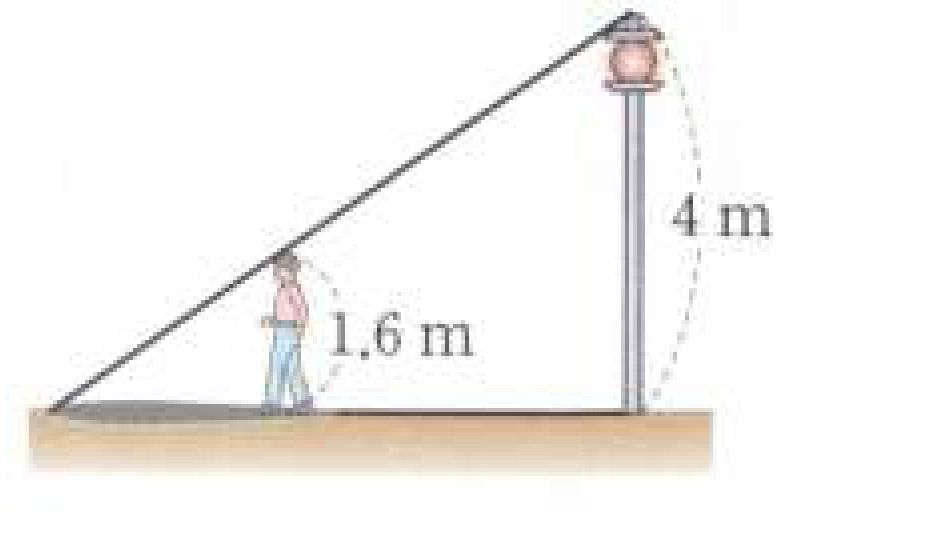
\includegraphics[width=0.92\linewidth]{figures/fig-86-69.jpg}\end{minipage}\par
\begin{choices32}{$1\mkern3mu \mathrm{m/s}$}{$1.2\mkern3mu \mathrm{m/s}$}{$1.5\mkern3mu \mathrm{m/s}$}{$1.8\mkern3mu \mathrm{m/s}$}{$2\mkern3mu \mathrm{m/s}$}\end{choices32}
}\vspace{8mm}
\setcounter{dmproblemcount}{69}\dmpnum{86-70}{% id: 86-70
% book: 쎈B 미적분1 · 06 도함수의 활용 (3)
% section: 유형 17 시각에 대한 길이의 변화율
% figure: tikz:fig-86-70
% answer: 
% answer_source: 
% variant_level: 0 (원본 전사)
% 이 파일은 build.mjs 가 items.json 에서 만든다. 고칠 때는 items.json 을 고친다.
\smash{\raisebox{1.5mm}{\dmkichul{쎈B 미적분1 86쪽 70번 · 서술형}}}
\noindent\begin{minipage}[t]{0.58\linewidth}\vspace{0pt}\raggedright 오른쪽 그림과 같이 좌표평면 위의 원점~$\pt{O}$를 동시에 출발하여 각각 $x$축, $y$축 위를 움직이는 두 점~$\pt{P}$, $\pt{Q}$가 있다. 점~$\pt{P}$는 $x$축의 양의 방향으로 매초 $3$의 속력으로 움직이고, 점~$\pt{Q}$는 $y$축의 양의 방향으로 매초 $1$의 속력으로 움직인다고 한다. 선분~$\pt{PQ}$와 직선 $y=2x$가 만나는 점을 $\pt{R}$라 할 때, 선분~$\pt{OR}$의 길이의 변화율을 구하시오.\end{minipage}\hfill\begin{minipage}[t]{0.4\linewidth}\vspace{0pt}\centering \resizebox{\ifdim\width>\linewidth\linewidth\else\width\fi}{!}{% 86-70(86쪽) — 좌표평면 위의 두 점 P(x축), Q(y축)와 직선 y=2x, 선분 PQ 가 직선과 만나는 점 R. 스캔 화질이 낮아 TikZ 로 다시 그림.
% 원문에 있는 것만: 직선 y=2x · 선분 PQ · 점 P·Q 의 찬 점 · 두 점이 움직이는 방향을 가리키는 화살표 · 라벨 y=2x, O, P, Q, R, x, y.
% 좌표·눈금은 원문에 없으므로 넣지 않는다(선분 OR 의 길이의 변화율이 그림에서 읽히지 않게).
\begin{tikzpicture}[x=0.70cm, y=0.70cm, line width=0.55pt]
  \draw[->, >=stealth, line width=0.7pt] (-0.70,0) -- (3.90,0) node[below=1pt, font=\small] {$x$};
  \draw[->, >=stealth, line width=0.7pt] (0,-1.15) -- (0,1.90) node[left=1pt, font=\small] {$y$};
  % 직선 y=2x
  \draw[line width=0.6pt] (-0.52,-1.04) -- (0.86,1.72);
  % 선분 PQ
  \draw[line width=0.6pt] (0,1) -- (3.05,0);
  \fill (0,1) circle (2.2pt);
  \fill (3.05,0) circle (2.2pt);
  % 움직이는 방향(원문의 화살표)
  \draw[->, >=stealth, red, line width=0.7pt] (-0.22,0.02) -- (-0.22,0.60);
  \draw[->, >=stealth, red, line width=0.7pt] (1.30,-0.26) -- (2.05,-0.26);
  \node[below right=-2pt and 0pt, font=\small] at (0,0) {$\pt{O}$};
  \node[anchor=east, inner sep=3pt, font=\small] at (0,1) {$\pt{Q}$};
  \node[below=3pt, font=\small] at (3.05,0) {$\pt{P}$};
  \node[anchor=north west, inner sep=1.5pt, font=\small] at (0.47,0.82) {$\pt{R}$};
  \node[anchor=west, font=\small] at (0.72,1.80) {$y=2x$};
\end{tikzpicture}
}\end{minipage}\par
}\vspace{8mm}
\dmsection{유형 18 시각에 대한 넓이의 변화율}
\setcounter{dmproblemcount}{70}\dmpnum{86-71}{% id: 86-71
% book: 쎈B 미적분1 · 06 도함수의 활용 (3)
% section: 유형 18 시각에 대한 넓이의 변화율
% figure: none
% answer: 
% answer_source: 
% variant_level: 0 (원본 전사)
% 이 파일은 build.mjs 가 items.json 에서 만든다. 고칠 때는 items.json 을 고친다.
\smash{\raisebox{1.5mm}{\dmkichul{쎈B 미적분1 86쪽 71번 · 대표 문제}}}
잔잔한 호수에 돌을 던지면 동심원 모양의 원이 생긴다. 가장 바깥쪽 원의 반지름의 길이가 매초 $7\mkern3mu \mathrm{cm}$씩 길어질 때, 돌을 던진 지 $3$초 후의 가장 바깥쪽 원의 넓이의 변화율을 $a\pi\mkern3mu \mathrm{cm}^2/\mathrm{s}$라 하자. 이때 상수 $a$의 값을 구하시오.
}\vspace{8mm}
\setcounter{dmproblemcount}{71}\dmpnum{87-72}{% id: 87-72
% book: 쎈B 미적분1 · 06 도함수의 활용 (3)
% section: 유형 18 시각에 대한 넓이의 변화율
% figure: none
% answer: 
% answer_source: 
% variant_level: 0 (원본 전사)
% 이 파일은 build.mjs 가 items.json 에서 만든다. 고칠 때는 items.json 을 고친다.
\smash{\raisebox{1.5mm}{\dmkichul{쎈B 미적분1 87쪽 72번}}}
가로, 세로의 길이가 각각 $10\mkern3mu \mathrm{cm}$, $6\mkern3mu \mathrm{cm}$인 직사각형의 각 변의 길이가 매초 $2\mkern3mu \mathrm{cm}$씩 길어질 때, 직사각형의 넓이가 $320\mkern3mu \mathrm{cm}^2$가 되는 순간의 넓이의 변화율은?
\begin{choices32}{$56\mkern3mu \mathrm{cm}^2/\mathrm{s}$}{$64\mkern3mu \mathrm{cm}^2/\mathrm{s}$}{$72\mkern3mu \mathrm{cm}^2/\mathrm{s}$}{$80\mkern3mu \mathrm{cm}^2/\mathrm{s}$}{$88\mkern3mu \mathrm{cm}^2/\mathrm{s}$}\end{choices32}
}\vspace{8mm}
\vspace{3mm}\setcounter{dmproblemcount}{72}\dmpnum{87-73}{% id: 87-73
% book: 쎈B 미적분1 · 06 도함수의 활용 (3)
% section: 유형 18 시각에 대한 넓이의 변화율
% figure: tikz:fig-87-73
% answer: 
% answer_source: 
% variant_level: 0 (원본 전사)
% 이 파일은 build.mjs 가 items.json 에서 만든다. 고칠 때는 items.json 을 고친다.
\smash{\raisebox{4.5mm}{\dmkichul{쎈B 미적분1 87쪽 73번 · 서술형}}}
다음 그림과 같이 길이가 $20$인 선분~$\pt{AB}$ 위의 한 점~$\pt{P}$가 점~$\pt{A}$에서 출발하여 점~$\pt{B}$를 향해 매초 $4$씩 움직인다. 출발한 지 $\dfrac{7}{2}$초 후의 선분~$\pt{AP}$, $\pt{BP}$를 각각 지름으로 하는 두 원의 넓이의 합의 변화율을 구하시오.
\par\smallskip\begin{center}\resizebox{\ifdim\width>\linewidth\linewidth\else\width\fi}{!}{% 87-73(87쪽) — 길이 20인 선분 AB 위의 점 P와, AP·BP 를 각각 지름으로 하는 두 원. 스캔 삽화라 TikZ 로 다시 그림.
% 원문에 있는 것만: 두 원 · 선분 AB · 20 을 가리키는 파선 호 · 점 P 와 P가 움직이는 방향 화살표 · 라벨 A, P, B.
% 원문 그림의 비율(큰 원이 작은 원보다 훨씬 크다)만 옮기고 AP·BP 의 값은 적지 않는다.
\begin{tikzpicture}[x=0.115cm, y=0.115cm, line width=0.55pt]
  \fill[orange!25] (7,0) circle (7);
  \fill[orange!25] (17,0) circle (3);
  \draw[line width=0.6pt] (7,0) circle (7);
  \draw[line width=0.6pt] (17,0) circle (3);
  \draw[line width=0.6pt] (0,0) -- (20,0);
  \draw[densely dashed, line width=0.45pt] (0,0) .. controls (6.5,3.4) .. (20,0);
  \fill (14,0) circle (2.2pt);
  \draw[->, >=stealth, red, line width=0.8pt] (14.6,-1.0) -- (17.2,-1.0);
  \node[anchor=east, inner sep=2.5pt, font=\small] at (0,0) {$\pt{A}$};
  \node[anchor=north east, inner sep=1.5pt, font=\small] at (14,-0.3) {$\pt{P}$};
  \node[anchor=west, inner sep=2.5pt, font=\small] at (20,0) {$\pt{B}$};
  \node[anchor=south, inner sep=1.5pt, font=\small, fill=orange!25] at (6.5,1.1) {$20$};
\end{tikzpicture}
}\end{center}
}\vspace{8mm}
\setcounter{dmproblemcount}{73}\dmpnum{87-74}{% id: 87-74
% book: 쎈B 미적분1 · 06 도함수의 활용 (3)
% section: 유형 18 시각에 대한 넓이의 변화율
% figure: tikz:fig-87-74
% answer: 
% answer_source: 
% variant_level: 0 (원본 전사)
% 이 파일은 build.mjs 가 items.json 에서 만든다. 고칠 때는 items.json 을 고친다.
\smash{\raisebox{1.5mm}{\dmkichul{쎈B 미적분1 87쪽 74번}}}
\noindent\begin{minipage}[t]{0.58\linewidth}\vspace{0pt}\raggedright 오른쪽 그림과 같이 $\seg{AB}=8$, $\seg{BC}=9$, $\angle\pt{B}=45^\circ$인 삼각형~$\pt{ABC}$에서 점~$\pt{P}$는 점~$\pt{A}$에서 출발하여 점~$\pt{B}$를 향해 매초 $1$씩 움직이고, 점~$\pt{Q}$는 점~$\pt{B}$에서 출발하여 점~$\pt{C}$를 향해 매초 $3$씩 움직인다. 두 점~$\pt{P}$, $\pt{Q}$가 동시에 출발한 지 $2$초 후의 삼각형~$\pt{PBQ}$의 넓이의 변화율을 구하시오.\end{minipage}\hfill\begin{minipage}[t]{0.4\linewidth}\vspace{0pt}\centering \resizebox{\ifdim\width>\linewidth\linewidth\else\width\fi}{!}{% 87-74(87쪽) — AB=8, BC=9, ∠B=45°인 삼각형 ABC 와 변 AB·BC 위를 움직이는 두 점 P, Q(삼각형 PBQ 색칠). 스캔 화질이 낮아 TikZ 로 다시 그림.
% 원문에 있는 것만: 삼각형 ABC · 선분 PQ · 색칠한 삼각형 PBQ · 8 과 9 를 가리키는 파선 호 · 45° 표시 · 두 점이 움직이는 방향 화살표 · 라벨 A, B, C, P, Q.
% BP·BQ 의 값은 원문에 없으므로 적지 않는다(2초 후의 넓이의 변화율이 그림에서 읽히지 않게).
\begin{tikzpicture}[x=0.38cm, y=0.38cm, line width=0.55pt]
  \fill[violet!15] (0,0) -- (4.243,4.243) -- (6,0) -- cycle;
  \draw[line width=0.6pt] (0,0) -- (5.657,5.657) -- (9,0) -- cycle;
  \draw[line width=0.6pt] (4.243,4.243) -- (6,0);
  % 45° 표시
  \draw[line width=0.45pt] (1.25,0) arc (0:45:1.25);
  \node[anchor=west, inner sep=1pt, font=\small] at (1.40,0.58) {$45^\circ$};
  % 8 · 9 를 가리키는 파선 호
  \draw[densely dashed, line width=0.45pt] (0,0) .. controls (1.15,4.30) .. (5.657,5.657);
  \draw[densely dashed, line width=0.45pt] (0,0) .. controls (4.5,-2.05) .. (9,0);
  \node[font=\small] at (1.30,2.05) {$8$};
  \node[font=\small] at (4.50,-1.60) {$9$};
  % 두 점이 움직이는 방향(원문의 화살표)
  \draw[->, >=stealth, red, line width=0.7pt] (5.52,4.80) -- (4.88,4.16);
  \draw[->, >=stealth, red, line width=0.7pt] (1.35,-0.45) -- (2.75,-0.45);
  \fill (4.243,4.243) circle (2.2pt);
  \fill (6,0) circle (2.2pt);
  \node[anchor=south, inner sep=3pt, font=\small] at (5.657,5.657) {$\pt{A}$};
  \node[anchor=east, inner sep=3pt, font=\small] at (0,0) {$\pt{B}$};
  \node[anchor=west, inner sep=3pt, font=\small] at (9,0) {$\pt{C}$};
  \node[anchor=south east, inner sep=1.5pt, font=\small] at (4.243,4.243) {$\pt{P}$};
  \node[anchor=north, inner sep=3pt, font=\small] at (6,0) {$\pt{Q}$};
\end{tikzpicture}
}\end{minipage}\par
}\vspace{8mm}
\dmsection{유형 19 시각에 대한 부피의 변화율}
\vspace{3mm}\setcounter{dmproblemcount}{74}\dmpnum{87-75}{% id: 87-75
% book: 쎈B 미적분1 · 06 도함수의 활용 (3)
% section: 유형 19 시각에 대한 부피의 변화율
% figure: none
% answer: 
% answer_source: 
% variant_level: 0 (원본 전사)
% 이 파일은 build.mjs 가 items.json 에서 만든다. 고칠 때는 items.json 을 고친다.
\smash{\raisebox{4.5mm}{\dmkichul{쎈B 미적분1 87쪽 75번 · 대표 문제}}}
반지름의 길이가 $3\mkern3mu \mathrm{cm}$인 구 모양의 고무풍선에 공기를 넣어서 반지름의 길이가 매초 $\dfrac{1}{3}\mkern3mu \mathrm{cm}$씩 늘어나고 있다. $3$초 후의 고무풍선의 부피의 변화율은?
\begin{choices32}{\rule[-3ex]{0pt}{8ex}$20\pi\mkern3mu \mathrm{cm}^3/\mathrm{s}$}{\rule[-3ex]{0pt}{8ex}$\dfrac{62}{3}\pi\mkern3mu \mathrm{cm}^3/\mathrm{s}$}{\rule[-3ex]{0pt}{8ex}$\dfrac{64}{3}\pi\mkern3mu \mathrm{cm}^3/\mathrm{s}$}{\rule[-3ex]{0pt}{8ex}$22\pi\mkern3mu \mathrm{cm}^3/\mathrm{s}$}{\rule[-3ex]{0pt}{8ex}$\dfrac{68}{3}\pi\mkern3mu \mathrm{cm}^3/\mathrm{s}$}\end{choices32}
}\vspace{8mm}
\setcounter{dmproblemcount}{75}\dmpnum{87-76}{% id: 87-76
% book: 쎈B 미적분1 · 06 도함수의 활용 (3)
% section: 유형 19 시각에 대한 부피의 변화율
% figure: none
% answer: 
% answer_source: 
% variant_level: 0 (원본 전사)
% 이 파일은 build.mjs 가 items.json 에서 만든다. 고칠 때는 items.json 을 고친다.
\smash{\raisebox{1.5mm}{\dmkichul{쎈B 미적분1 87쪽 76번 · 서술형}}}
밑면은 한 변의 길이가 $4\mkern3mu \mathrm{cm}$인 정사각형이고 높이는 $10\mkern3mu \mathrm{cm}$인 직육면체가 있다. 이 직육면체의 밑면의 각 변의 길이는 매초 $1\mkern3mu \mathrm{cm}$씩 길어지고 높이는 매초 $2\mkern3mu \mathrm{cm}$씩 짧아진다. 이 직육면체의 부피의 변화율이 $0$이 될 때, 직육면체의 부피를 구하시오.
}\vspace{8mm}
\vspace{3mm}\setcounter{dmproblemcount}{76}\dmpnum{87-77}{% id: 87-77
% book: 쎈B 미적분1 · 06 도함수의 활용 (3)
% section: 유형 19 시각에 대한 부피의 변화율
% figure: crop:fig-87-77.jpg
% answer: 
% answer_source: 
% variant_level: 0 (원본 전사)
% 이 파일은 build.mjs 가 items.json 에서 만든다. 고칠 때는 items.json 을 고친다.
\smash{\raisebox{4.5mm}{\dmkichul{쎈B 미적분1 87쪽 77번}}}
\noindent\begin{minipage}[t]{0.58\linewidth}\vspace{0pt}\raggedright 밑면의 반지름의 길이가 $8\mkern3mu \mathrm{cm}$, 높이가 $16\mkern3mu \mathrm{cm}$인 원뿔 모양의 빈 그릇에 오른쪽 그림과 같이 매초 $\dfrac{3}{2}\mkern3mu \mathrm{cm}$씩 수면의 높이가 올라가도록 물을 넣는다. 수면의 높이가 $12\mkern3mu \mathrm{cm}$가 되는 순간의 물의 부피의 변화율을 $a\pi\mkern3mu \mathrm{cm}^3/\mathrm{s}$라 할 때, 상수 $a$의 값은?\end{minipage}\hfill\begin{minipage}[t]{0.4\linewidth}\vspace{0pt}\centering 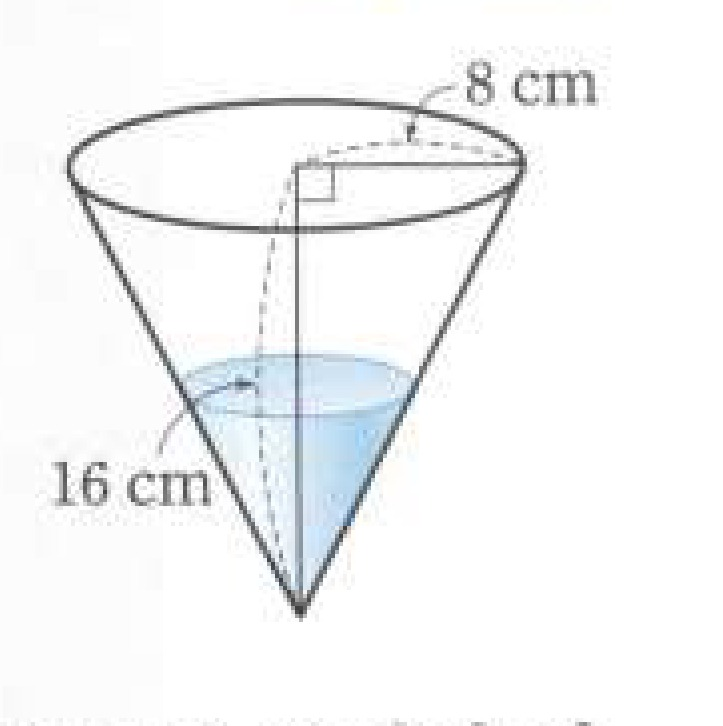
\includegraphics[width=0.92\linewidth]{figures/fig-87-77.jpg}\end{minipage}\par
\dmchoicesauto{}{$36$}{$42$}{$48$}{$54$}{$60$}
}\vspace{8mm}
\vspace*{0pt plus 1filll}
\clearpage
\renewcommand{\dmchapunit}{07 부정적분}
\dmchapter{07}{부정적분}
\setcounter{dmproblemcount}{0}
\dmsection{유형 01 부정적분의 정의}
\vspace{3mm}\setcounter{dmproblemcount}{0}\dmpnum{91-01}{% id: 91-01
% book: 쎈B 미적분1 · 07 부정적분
% section: 유형 01 부정적분의 정의
% figure: none
% answer: 
% answer_source: 
% variant_level: 0 (원본 전사)
% 이 파일은 build.mjs 가 items.json 에서 만든다. 고칠 때는 items.json 을 고친다.
\smash{\raisebox{4.5mm}{\dmkichul{쎈B 미적분1 91쪽 01번 · 대표 문제}}}
다항함수 $f(x)$에 대하여\par\smallskip\dispeq{$\displaystyle\int (x-1)f(x)\mkern3mu dx=x^3+6x^2-15x+C$}\par\smallskip\noindent 가 성립할 때, $f(1)$의 값을 구하시오. \dmcondfill{$C$는 적분상수이다.}{}
}\vspace{8mm}
\setcounter{dmproblemcount}{1}\dmpnum{91-02}{% id: 91-02
% book: 쎈B 미적분1 · 07 부정적분
% section: 유형 01 부정적분의 정의
% figure: none
% answer: 
% answer_source: 
% variant_level: 0 (원본 전사)
% 이 파일은 build.mjs 가 items.json 에서 만든다. 고칠 때는 items.json 을 고친다.
\smash{\raisebox{1.5mm}{\dmkichul{쎈B 미적분1 91쪽 02번}}}
함수 $f(x)$의 부정적분 중 하나가 $2x^2-3x+1$일 때, $f(2)$의 값을 구하시오.
}\vspace{8mm}
\setcounter{dmproblemcount}{2}\dmpnum{91-03}{% id: 91-03
% book: 쎈B 미적분1 · 07 부정적분
% section: 유형 01 부정적분의 정의
% figure: none
% answer: 
% answer_source: 
% variant_level: 0 (원본 전사)
% 이 파일은 build.mjs 가 items.json 에서 만든다. 고칠 때는 items.json 을 고친다.
\smash{\raisebox{1.5mm}{\dmkichul{쎈B 미적분1 91쪽 03번}}}
두 함수 $F(x)$, $G(x)$가 모두 함수 $f(x)$의 부정적분이고 $F(2)=5$, $G(2)=-2$일 때, $F(3)-G(3)$의 값은?
\dmchoicesauto{}{$1$}{$3$}{$5$}{$7$}{$9$}
}\vspace{8mm}
\setcounter{dmproblemcount}{3}\dmpnum{91-04}{% id: 91-04
% book: 쎈B 미적분1 · 07 부정적분
% section: 유형 01 부정적분의 정의
% figure: none
% answer: 
% answer_source: 
% variant_level: 0 (원본 전사)
% 이 파일은 build.mjs 가 items.json 에서 만든다. 고칠 때는 items.json 을 고친다.
\smash{\raisebox{1.5mm}{\dmkichul{쎈B 미적분1 91쪽 04번 · 서술형}}}
함수 $F(x)=x^3+ax^2+bx$가 함수 $f(x)$의 부정적분 중 하나이고 $f(0)=-1$, $f'(0)=2$일 때, 상수 $a$, $b$에 대하여 $ab$의 값을 구하시오.
}\vspace{8mm}
\setcounter{dmproblemcount}{4}\dmpnum{91-05}{% id: 91-05
% book: 쎈B 미적분1 · 07 부정적분
% section: 유형 01 부정적분의 정의
% figure: none
% answer: 
% answer_source: 
% variant_level: 0 (원본 전사)
% 이 파일은 build.mjs 가 items.json 에서 만든다. 고칠 때는 items.json 을 고친다.
\smash{\raisebox{1.5mm}{\dmkichul{쎈B 미적분1 91쪽 05번}}}
함수 $f(x)$의 한 부정적분 $F(x)$와 또 다른 부정적분 $G(x)$에 대하여\par\smallskip\dispeq{$F(x)=x^3+2x^2-x+3$, $G(1)=2$}\par\smallskip\noindent 일 때, $G(-1)$의 값을 구하시오.
}\vspace{8mm}
\vspace{3mm}\setcounter{dmproblemcount}{5}\dmpnum{91-06}{% id: 91-06
% book: 쎈B 미적분1 · 07 부정적분
% section: 유형 01 부정적분의 정의
% figure: none
% answer: 
% answer_source: 
% variant_level: 0 (원본 전사)
% 이 파일은 build.mjs 가 items.json 에서 만든다. 고칠 때는 items.json 을 고친다.
\smash{\raisebox{4.5mm}{\dmkichul{쎈B 미적분1 91쪽 06번}}}
두 함수 $f(x)=2x^2-x$, $g(x)=x^2+3$에 대하여\par\smallskip\dispeq{$\displaystyle\int \{x+h(x)\}\mkern3mu dx=f(x)g(x)$}\par\smallskip\noindent 를 만족시키는 함수 $h(x)$의 일차항의 계수는?
\dmchoicesauto{}{$7$}{$8$}{$9$}{$10$}{$11$}
}\vspace{8mm}
\dmsection{유형 02 부정적분과 미분의 관계; $\frac{d}{dx}\int f(x)dx=f(x)$}
\vspace{3mm}\setcounter{dmproblemcount}{6}\dmpnum{91-07}{% id: 91-07
% book: 쎈B 미적분1 · 07 부정적분
% section: 유형 02 부정적분과 미분의 관계; $\frac{d}{dx}\int f(x)dx=f(x)$
% figure: none
% answer: 
% answer_source: 
% variant_level: 0 (원본 전사)
% 이 파일은 build.mjs 가 items.json 에서 만든다. 고칠 때는 items.json 을 고친다.
\smash{\raisebox{4.5mm}{\dmkichul{쎈B 미적분1 91쪽 07번 · 대표 문제}}}
함수 $f(x)=4x^3-x^2+5x-2$에 대하여\par\smallskip\dispeq{$F(x)=\dfrac{d}{dx}\displaystyle\int xf(x)\mkern3mu dx$}\par\smallskip\noindent 일 때, $F(1)$의 값은?
\dmchoicesauto{}{$6$}{$8$}{$10$}{$12$}{$14$}
}\vspace{8mm}
\vspace{3mm}\setcounter{dmproblemcount}{7}\dmpnum{92-08}{% id: 92-08
% book: 쎈B 미적분1 · 07 부정적분
% section: 유형 02 부정적분과 미분의 관계; $\frac{d}{dx}\int f(x)dx=f(x)$
% figure: none
% answer: 
% answer_source: 
% variant_level: 0 (원본 전사)
% 이 파일은 build.mjs 가 items.json 에서 만든다. 고칠 때는 items.json 을 고친다.
\smash{\raisebox{4.5mm}{\dmkichul{쎈B 미적분1 92쪽 08번}}}
모든 실수 $x$에 대하여\par\smallskip\dispeq{$\dfrac{d}{dx}\displaystyle\int (x^2+ax+8)\mkern3mu dx=bx^2-2x+c$}\par\smallskip\noindent 가 성립할 때, 상수 $a$, $b$, $c$에 대하여 $a+b+c$의 값은?
\dmchoicesauto{}{$1$}{$3$}{$5$}{$7$}{$9$}
}\vspace{8mm}
\vspace{3mm}\setcounter{dmproblemcount}{8}\dmpnum{92-09}{% id: 92-09
% book: 쎈B 미적분1 · 07 부정적분
% section: 유형 02 부정적분과 미분의 관계; $\frac{d}{dx}\int f(x)dx=f(x)$
% figure: none
% answer: 
% answer_source: 
% variant_level: 0 (원본 전사)
% 이 파일은 build.mjs 가 items.json 에서 만든다. 고칠 때는 items.json 을 고친다.
\smash{\raisebox{4.5mm}{\dmkichul{쎈B 미적분1 92쪽 09번}}}
방정식\par\smallskip\dispeq{$\dfrac{d}{dx}\displaystyle\int (x^3-5x+1)\mkern3mu dx-\dfrac{d}{dx}\displaystyle\int (2x^2-5)\mkern3mu dx=0$}\par\smallskip\noindent 의 모든 근의 합은?
\dmchoicesauto{}{$-2$}{$-1$}{$0$}{$1$}{$2$}
}\vspace{8mm}
\dmsection{유형 03 부정적분과 미분의 관계; $\int\left\{\frac{d}{dx}f(x)\right\}dx=f(x)+C$}
\vspace{3mm}\setcounter{dmproblemcount}{9}\dmpnum{92-10}{% id: 92-10
% book: 쎈B 미적분1 · 07 부정적분
% section: 유형 03 부정적분과 미분의 관계; $\int\left\{\frac{d}{dx}f(x)\right\}dx=f(x)+C$
% figure: none
% answer: 
% answer_source: 
% variant_level: 0 (원본 전사)
% 이 파일은 build.mjs 가 items.json 에서 만든다. 고칠 때는 items.json 을 고친다.
\smash{\raisebox{4.5mm}{\dmkichul{쎈B 미적분1 92쪽 10번 · 대표 문제}}}
함수 \par\smallskip\dispeq{$F(x)=\displaystyle\int \Big\{\dfrac{d}{dx}(2x^3+x^2-x)\Big\}\mkern3mu dx$}\par\smallskip\noindent 에 대하여 $F(0)=3$일 때, $F(1)$의 값은?
\dmchoicesauto{}{$1$}{$2$}{$3$}{$4$}{$5$}
}\vspace{8mm}
\vspace{3mm}\setcounter{dmproblemcount}{10}\dmpnum{92-11}{% id: 92-11
% book: 쎈B 미적분1 · 07 부정적분
% section: 유형 03 부정적분과 미분의 관계; $\int\left\{\frac{d}{dx}f(x)\right\}dx=f(x)+C$
% figure: none
% answer: 
% answer_source: 
% variant_level: 0 (원본 전사)
% 이 파일은 build.mjs 가 items.json 에서 만든다. 고칠 때는 items.json 을 고친다.
\smash{\raisebox{4.5mm}{\dmkichul{쎈B 미적분1 92쪽 11번 · 서술형}}}
함수 $f(x)=x^3-3x$에 대하여 두 함수 $g(x)$, $h(x)$를\par\smallskip\dispeq{$g(x)=\dfrac{d}{dx}\displaystyle\int f(x)\mkern3mu dx$, $h(x)=\displaystyle\int \Big\{\dfrac{d}{dx}f(x)\Big\}\mkern3mu dx$}\par\smallskip\noindent 로 정의하자. $h(2)=4$일 때, $g(-2)+h(1)$의 값을 구하시오.
}\vspace{8mm}
\vspace{3mm}\setcounter{dmproblemcount}{11}\dmpnum{92-12}{% id: 92-12
% book: 쎈B 미적분1 · 07 부정적분
% section: 유형 03 부정적분과 미분의 관계; $\int\left\{\frac{d}{dx}f(x)\right\}dx=f(x)+C$
% figure: none
% answer: 
% answer_source: 
% variant_level: 0 (원본 전사)
% 이 파일은 build.mjs 가 items.json 에서 만든다. 고칠 때는 items.json 을 고친다.
\smash{\raisebox{4.5mm}{\dmkichul{쎈B 미적분1 92쪽 12번}}}
다항함수 $f(x)$에 대하여\par\smallskip\dispeq{$\dfrac{d}{dx}\displaystyle\int \{f(x)+4x^3-x^2\}\mkern3mu dx$}\par\smallskip\dispeq{$=\displaystyle\int \Big[\dfrac{d}{dx}\{3f(x)+2x^3+x^2-6x\}\Big]\mkern3mu dx$}\par\smallskip\noindent 가 성립한다. $f(1)=4$일 때, $f(0)$의 값은?
\dmchoicesauto{}{$1$}{$3$}{$5$}{$7$}{$9$}
}\vspace{8mm}
\vspace{3mm}\setcounter{dmproblemcount}{12}\dmpnum{92-13}{% id: 92-13
% book: 쎈B 미적분1 · 07 부정적분
% section: 유형 03 부정적분과 미분의 관계; $\int\left\{\frac{d}{dx}f(x)\right\}dx=f(x)+C$
% figure: none
% answer: 
% answer_source: 
% variant_level: 0 (원본 전사)
% 이 파일은 build.mjs 가 items.json 에서 만든다. 고칠 때는 items.json 을 고친다.
\smash{\raisebox{4.5mm}{\dmkichul{쎈B 미적분1 92쪽 13번}}}
함수 $f(x)=\displaystyle\int \Big\{\dfrac{d}{dx}(2x^2-x)\Big\}\mkern3mu dx$의 최솟값이 $\dfrac{7}{8}$일 때, $f(-1)$의 값을 구하시오.
}\vspace{8mm}
\vspace{3mm}\setcounter{dmproblemcount}{13}\dmpnum{92-14}{% id: 92-14
% book: 쎈B 미적분1 · 07 부정적분
% section: 유형 03 부정적분과 미분의 관계; $\int\left\{\frac{d}{dx}f(x)\right\}dx=f(x)+C$
% figure: none
% answer: 
% answer_source: 
% variant_level: 0 (원본 전사)
% 이 파일은 build.mjs 가 items.json 에서 만든다. 고칠 때는 items.json 을 고친다.
\smash{\raisebox{4.5mm}{\dmkichul{쎈B 미적분1 92쪽 14번}}}
함수 $f(x)=100x^{100}+99x^{99}+\cdots+2x^2+x$에 대하여\par\smallskip\dispeq{$F(x)=\displaystyle\int \Big[\dfrac{d}{dx}\displaystyle\int \Big\{\dfrac{d}{dx}f(x)\Big\}\mkern3mu dx\Big]\mkern3mu dx$}\par\smallskip\noindent 이고 $F(0)=-1$일 때, $F(1)$의 값을 구하시오.
}\vspace{8mm}
\dmsection{유형 04 부정적분과 미분의 관계를 이용하여 함수 구하기}
\vspace{3mm}\setcounter{dmproblemcount}{14}\dmpnum{93-15}{% id: 93-15
% book: 쎈B 미적분1 · 07 부정적분
% section: 유형 04 부정적분과 미분의 관계를 이용하여 함수 구하기
% figure: none
% answer: 
% answer_source: 
% variant_level: 0 (원본 전사)
% 이 파일은 build.mjs 가 items.json 에서 만든다. 고칠 때는 items.json 을 고친다.
\smash{\raisebox{4.5mm}{\dmkichul{쎈B 미적분1 93쪽 15번 · 대표 문제}}}
다항함수 $f(x)$의 도함수 $f'(x)$에 대하여\par\smallskip\dispeq{$\displaystyle\int (x-1)f'(x)\mkern3mu dx=\dfrac{2}{3}x^3+\dfrac{5}{2}x^2-7x$}\par\smallskip\noindent 가 성립한다. $f(1)=4$일 때, 방정식 $f(x)=0$의 모든 근의 곱은?
\dmchoicesauto{}{$-5$}{$-4$}{$-3$}{$-2$}{$-1$}
}\vspace{8mm}
\vspace{3mm}\setcounter{dmproblemcount}{15}\dmpnum{93-16}{% id: 93-16
% book: 쎈B 미적분1 · 07 부정적분
% section: 유형 04 부정적분과 미분의 관계를 이용하여 함수 구하기
% figure: none
% answer: 
% answer_source: 
% variant_level: 0 (원본 전사)
% 이 파일은 build.mjs 가 items.json 에서 만든다. 고칠 때는 items.json 을 고친다.
\smash{\raisebox{4.5mm}{\dmkichul{쎈B 미적분1 93쪽 16번}}}
다항함수 $f(x)$에 대하여\par\smallskip\dispeq{$\displaystyle\int \{f(x)-x\}\mkern3mu dx=x^3+ax^2+bx+C$}\par\smallskip\noindent 가 성립한다. $f(0)=8$, $f'(1)=1$일 때, $f(-1)$의 값은? \dmcondfill{$a$, $b$는 상수이고, $C$는 적분상수이다.}{}
\dmchoicesauto{}{$8$}{$10$}{$12$}{$14$}{$16$}
}\vspace{8mm}
\vspace{3mm}\setcounter{dmproblemcount}{16}\dmpnum{93-17}{% id: 93-17
% book: 쎈B 미적분1 · 07 부정적분
% section: 유형 04 부정적분과 미분의 관계를 이용하여 함수 구하기
% figure: none
% answer: 
% answer_source: 
% variant_level: 0 (원본 전사)
% 이 파일은 build.mjs 가 items.json 에서 만든다. 고칠 때는 items.json 을 고친다.
\smash{\raisebox{4.5mm}{\dmkichul{쎈B 미적분1 93쪽 17번 · 서술형}}}
두 일차함수 $f(x)$, $g(x)$에 대하여\par\smallskip\dispeq{$\dfrac{d}{dx}\{f(x)+g(x)\}=6$, $\dfrac{d}{dx}\{f(x)g(x)\}=16x-2$}\par\smallskip\noindent 이고 $f(0)=1$, $g(0)=-3$일 때, $f(3)-g(3)$의 값을 구하시오.
}\vspace{8mm}
\dmsection{유형 05 부정적분의 계산}
\vspace{3mm}\setcounter{dmproblemcount}{17}\dmpnum{93-18}{% id: 93-18
% book: 쎈B 미적분1 · 07 부정적분
% section: 유형 05 부정적분의 계산
% figure: none
% answer: 
% answer_source: 
% variant_level: 0 (원본 전사)
% 이 파일은 build.mjs 가 items.json 에서 만든다. 고칠 때는 items.json 을 고친다.
\smash{\raisebox{4.5mm}{\dmkichul{쎈B 미적분1 93쪽 18번 · 대표 문제}}}
함수 $f(x)$에 대하여\par\smallskip\dispeq{$\displaystyle f(x)=\int (3-\sqrt{x}\mkern3mu )^2\mkern3mu dx+\int (3+\sqrt{x}\mkern3mu )^2\mkern3mu dx$}\par\smallskip\noindent 이고 $f(1)=20$일 때, $f(0)$의 값을 구하시오.
}\vspace{8mm}
\vspace{3mm}\setcounter{dmproblemcount}{18}\dmpnum{93-19}{% id: 93-19
% book: 쎈B 미적분1 · 07 부정적분
% section: 유형 05 부정적분의 계산
% figure: none
% answer: 
% answer_source: 
% variant_level: 0 (원본 전사)
% 이 파일은 build.mjs 가 items.json 에서 만든다. 고칠 때는 items.json 을 고친다.
\smash{\raisebox{4.5mm}{\dmkichul{쎈B 미적분1 93쪽 19번}}}
함수 $f(x)$에 대하여\par\smallskip\dispeq{$\displaystyle f(x)=\int\Big(\dfrac{3}{4}x^3+7x-2\Big)\mkern3mu dx-\int\Big(\dfrac{3}{4}x^3+x\Big)\mkern3mu dx$}\par\smallskip\noindent 이고 $f(1)=5$일 때, $f(2)$의 값을 구하시오.
}\vspace{8mm}
\vspace{3mm}\setcounter{dmproblemcount}{19}\dmpnum{93-20}{% id: 93-20
% book: 쎈B 미적분1 · 07 부정적분
% section: 유형 05 부정적분의 계산
% figure: none
% answer: 
% answer_source: 
% variant_level: 0 (원본 전사)
% 이 파일은 build.mjs 가 items.json 에서 만든다. 고칠 때는 items.json 을 고친다.
\smash{\raisebox{4.5mm}{\dmkichul{쎈B 미적분1 93쪽 20번}}}
함수 $f(x)$에 대하여\par\smallskip\dispeq{$\displaystyle f(x)=\int \dfrac{x^3}{x-2}\mkern3mu dx-\int \dfrac{8}{x-2}\mkern3mu dx$}\par\smallskip\noindent 이고 $f(0)=\dfrac{2}{3}$일 때, $f(-2)$의 값을 구하시오.
}\vspace{8mm}
\vspace{3mm}\setcounter{dmproblemcount}{20}\dmpnum{93-21}{% id: 93-21
% book: 쎈B 미적분1 · 07 부정적분
% section: 유형 05 부정적분의 계산
% figure: none
% answer: 
% answer_source: 
% variant_level: 0 (원본 전사)
% 이 파일은 build.mjs 가 items.json 에서 만든다. 고칠 때는 items.json 을 고친다.
\smash{\raisebox{4.5mm}{\dmkichul{쎈B 미적분1 93쪽 21번}}}
함수 $f(x)$에 대하여\par\smallskip\dispeq{$\displaystyle f(x)=\int\Big(x+\dfrac{1}{2}x^2+\dfrac{1}{3}x^3+\cdots+\dfrac{1}{20}x^{20}\Big)\mkern3mu dx$}\par\smallskip\noindent 이고 $f(0)=0$일 때, $f(1)$의 값을 구하시오.
}\vspace{8mm}
\dmsection{유형 06 도함수가 주어질 때 함수 구하기}
\setcounter{dmproblemcount}{21}\dmpnum{94-22}{% id: 94-22
% book: 쎈B 미적분1 · 07 부정적분
% section: 유형 06 도함수가 주어질 때 함수 구하기
% figure: none
% answer: 
% answer_source: 
% variant_level: 0 (원본 전사)
% 이 파일은 build.mjs 가 items.json 에서 만든다. 고칠 때는 items.json 을 고친다.
\smash{\raisebox{1.5mm}{\dmkichul{쎈B 미적분1 94쪽 22번 · 대표 문제}}}
함수 $f(x)$에 대하여 $f'(x)=3x^2+2ax+2$이고 $f(1)=0$, $f(2)=-3$일 때, $f(-1)$의 값을 구하시오. \dmcondfill{$a$는 상수이다.}{}
}\vspace{8mm}
\setcounter{dmproblemcount}{22}\dmpnum{94-23}{% id: 94-23
% book: 쎈B 미적분1 · 07 부정적분
% section: 유형 06 도함수가 주어질 때 함수 구하기
% figure: none
% answer: 
% answer_source: 
% variant_level: 0 (원본 전사)
% 이 파일은 build.mjs 가 items.json 에서 만든다. 고칠 때는 items.json 을 고친다.
\smash{\raisebox{1.5mm}{\dmkichul{쎈B 미적분1 94쪽 23번}}}
함수 $f(x)$에 대하여 $f'(x)=6x^2-4$이고 함수 $y=f(x)$의 그래프가 점 $(0{,}\mkern3mu\mathopen{}8)$을 지날 때, $f(2)$의 값을 구하시오.
}\vspace{8mm}
\vspace{3mm}\setcounter{dmproblemcount}{23}\dmpnum{94-24}{% id: 94-24
% book: 쎈B 미적분1 · 07 부정적분
% section: 유형 06 도함수가 주어질 때 함수 구하기
% figure: none
% answer: 
% answer_source: 
% variant_level: 0 (원본 전사)
% 이 파일은 build.mjs 가 items.json 에서 만든다. 고칠 때는 items.json 을 고친다.
\smash{\raisebox{4.5mm}{\dmkichul{쎈B 미적분1 94쪽 24번}}}
함수 $f(x)$에 대하여 $f'(x)=\dfrac{x^4-1}{x^2+1}$이고 $f(1)=\dfrac{4}{3}$일 때, $f(3)$의 값은?
\dmchoicesauto{}{$2$}{$4$}{$6$}{$8$}{$10$}
}\vspace{8mm}
\setcounter{dmproblemcount}{24}\dmpnum{94-25}{% id: 94-25
% book: 쎈B 미적분1 · 07 부정적분
% section: 유형 06 도함수가 주어질 때 함수 구하기
% figure: none
% answer: 
% answer_source: 
% variant_level: 0 (원본 전사)
% 이 파일은 build.mjs 가 items.json 에서 만든다. 고칠 때는 items.json 을 고친다.
\smash{\raisebox{1.5mm}{\dmkichul{쎈B 미적분1 94쪽 25번 · 서술형}}}
함수 $f(x)$에 대하여 $f'(x)=6x^2-10x+k$이고 다항식 $f(x)$가 $x^2-2x-3$으로 나누어떨어질 때, $f(1)$의 값을 구하시오. \dmcondfill{$k$는 상수이다.}{}
}\vspace{8mm}
\vspace{5mm}\setcounter{dmproblemcount}{25}\dmpnum{94-26}{% id: 94-26
% book: 쎈B 미적분1 · 07 부정적분
% section: 유형 06 도함수가 주어질 때 함수 구하기
% figure: none
% answer: 
% answer_source: 
% variant_level: 0 (원본 전사)
% 이 파일은 build.mjs 가 items.json 에서 만든다. 고칠 때는 items.json 을 고친다.
\smash{\raisebox{6.5mm}{\dmkichul{쎈B 미적분1 94쪽 26번}}}
계수가 모두 정수인 두 다항함수 $f(x)$, $g(x)$에 대하여\par\smallskip\dispeq{$\begin{aligned} &f'(x)-g'(x)=-2x+6, \\ &f'(x)g(x)+f(x)g'(x)=3x^2-12x+7 \end{aligned}$}\par\smallskip\noindent 이고 $f(0)=-1$, $g(0)=2$일 때, $f(2)+g(1)$의 값은?
\dmchoicesauto{}{$-2$}{$-1$}{$0$}{$1$}{$2$}
}\vspace{8mm}
\dmsection{유형 07 함수와 부정적분 사이의 관계식이 주어질 때 함수 구하기}
\vspace{3mm}\setcounter{dmproblemcount}{26}\dmpnum{94-27}{% id: 94-27
% book: 쎈B 미적분1 · 07 부정적분
% section: 유형 07 함수와 부정적분 사이의 관계식이 주어질 때 함수 구하기
% figure: none
% answer: 
% answer_source: 
% variant_level: 0 (원본 전사)
% 이 파일은 build.mjs 가 items.json 에서 만든다. 고칠 때는 items.json 을 고친다.
\smash{\raisebox{4.5mm}{\dmkichul{쎈B 미적분1 94쪽 27번 · 대표 문제}}}
다항함수 $f(x)$에 대하여 $\dfrac{d}{dx}F(x)=f(x)$이고,\par\smallskip\dispeq{$F(x)=xf(x)-3x^4-2x^3$}\par\smallskip\noindent 이 성립한다. $f(-1)=1$일 때, 함수 $f(x)$를 구하시오.
}\vspace{8mm}
\vspace{3mm}\setcounter{dmproblemcount}{27}\dmpnum{95-28}{% id: 95-28
% book: 쎈B 미적분1 · 07 부정적분
% section: 유형 07 함수와 부정적분 사이의 관계식이 주어질 때 함수 구하기
% figure: none
% answer: 
% answer_source: 
% variant_level: 0 (원본 전사)
% 이 파일은 build.mjs 가 items.json 에서 만든다. 고칠 때는 items.json 을 고친다.
\smash{\raisebox{4.5mm}{\dmkichul{쎈B 미적분1 95쪽 28번}}}
미분가능한 함수 $f(x)$에 대하여 $f(1)=3$, $f'(1)=-1$이고 \par\smallskip\dispeq{$\displaystyle\int g(x)\mkern3mu dx=2x^2f(x)+C$}\par\smallskip\noindent 가 성립할 때, $g(1)$의 값은? \dmcondfill{$C$는 적분상수이다.}{}
\dmchoicesauto{}{$4$}{$6$}{$8$}{$10$}{$12$}
}\vspace{8mm}
\vspace{3mm}\setcounter{dmproblemcount}{28}\dmpnum{95-29}{% id: 95-29
% book: 쎈B 미적분1 · 07 부정적분
% section: 유형 07 함수와 부정적분 사이의 관계식이 주어질 때 함수 구하기
% figure: none
% answer: 
% answer_source: 
% variant_level: 0 (원본 전사)
% 이 파일은 build.mjs 가 items.json 에서 만든다. 고칠 때는 items.json 을 고친다.
\smash{\raisebox{4.5mm}{\dmkichul{쎈B 미적분1 95쪽 29번 · 서술형}}}
일차함수 $f(x)$에 대하여 \par\smallskip\dispeq{$\displaystyle 2\int f(x)\mkern3mu dx=f(x)+xf(x)+3x+1$}\par\smallskip\noindent 이 성립한다. 함수 $y=f(x)$의 그래프가 두 점 $(1{,}\mkern3mu\mathopen{}-1)$, $(2{,}\mkern3mu\mathopen{}k)$를 지날 때, $k$의 값을 구하시오.
}\vspace{8mm}
\vspace{3mm}\setcounter{dmproblemcount}{29}\dmpnum{95-30}{% id: 95-30
% book: 쎈B 미적분1 · 07 부정적분
% section: 유형 07 함수와 부정적분 사이의 관계식이 주어질 때 함수 구하기
% figure: none
% answer: 
% answer_source: 
% variant_level: 0 (원본 전사)
% 이 파일은 build.mjs 가 items.json 에서 만든다. 고칠 때는 items.json 을 고친다.
\smash{\raisebox{4.5mm}{\dmkichul{쎈B 미적분1 95쪽 30번}}}
다항함수 $f(x)$에 대하여 \par\smallskip\dispeq{$\displaystyle f(x)+\int xf(x)\mkern3mu dx=x^4-x^3-x^2-3x$}\par\smallskip\noindent 가 성립할 때, $f(1)$의 값은?
\dmchoicesauto{}{$-9$}{$-7$}{$1$}{$7$}{$9$}
}\vspace{8mm}
\dmsection{유형 08 부정적분과 함수의 연속성}
\vspace{5mm}\setcounter{dmproblemcount}{30}\dmpnum{95-31}{% id: 95-31
% book: 쎈B 미적분1 · 07 부정적분
% section: 유형 08 부정적분과 함수의 연속성
% figure: none
% answer: 
% answer_source: 
% variant_level: 0 (원본 전사)
% 이 파일은 build.mjs 가 items.json 에서 만든다. 고칠 때는 items.json 을 고친다.
\smash{\raisebox{6.5mm}{\dmkichul{쎈B 미적분1 95쪽 31번 · 대표 문제}}}
함수 $f(x)$의 도함수가 \par\smallskip\dispeq{$f'(x)=\begin{cases} 2x+1 & (x>1) \\ k & (x<1) \end{cases}$}\par\smallskip\noindent 이고 $f(-1)=-3$, $f(2)=5$일 때, $f(x)$가 $x=1$에서 연속이 되도록 하는 상수 $k$의 값은?
\dmchoicesauto{}{$1$}{$2$}{$3$}{$4$}{$5$}
}\vspace{8mm}
\vspace{5mm}\setcounter{dmproblemcount}{31}\dmpnum{95-32}{% id: 95-32
% book: 쎈B 미적분1 · 07 부정적분
% section: 유형 08 부정적분과 함수의 연속성
% figure: none
% answer: 
% answer_source: 
% variant_level: 0 (원본 전사)
% 이 파일은 build.mjs 가 items.json 에서 만든다. 고칠 때는 items.json 을 고친다.
\smash{\raisebox{6.5mm}{\dmkichul{쎈B 미적분1 95쪽 32번}}}
모든 실수 $x$에 대하여 미분가능한 함수 $f(x)$의 도함수가 \par\smallskip\dispeq{$f'(x)=\begin{cases} -4x^3+1 & (x\ge -1) \\ 3x^2+2 & (x<-1) \end{cases}$}\par\smallskip\noindent 이고 $f(0)=1$일 때, $f(-2)$의 값을 구하시오.
}\vspace{8mm}
\setcounter{dmproblemcount}{32}\dmpnum{95-33}{% id: 95-33
% book: 쎈B 미적분1 · 07 부정적분
% section: 유형 08 부정적분과 함수의 연속성
% figure: none
% answer: 
% answer_source: 
% variant_level: 0 (원본 전사)
% 이 파일은 build.mjs 가 items.json 에서 만든다. 고칠 때는 items.json 을 고친다.
\smash{\raisebox{1.5mm}{\dmkichul{쎈B 미적분1 95쪽 33번}}}
연속함수 $f(x)$의 도함수가 \par\smallskip\dispeq{$f'(x)=3x-|x|$}\par\smallskip\noindent 이고 $f(0)=1$일 때, $f(-2)f(3)$의 값을 구하시오.
}\vspace{8mm}
\setcounter{dmproblemcount}{33}\dmpnum{96-34}{% id: 96-34
% book: 쎈B 미적분1 · 07 부정적분
% section: 유형 08 부정적분과 함수의 연속성
% figure: tikz:fig-96-34
% answer: 
% answer_source: 
% variant_level: 0 (원본 전사)
% 이 파일은 build.mjs 가 items.json 에서 만든다. 고칠 때는 items.json 을 고친다.
\smash{\raisebox{1.5mm}{\dmkichul{쎈B 미적분1 96쪽 34번 · 서술형}}}
\noindent\begin{minipage}[t]{0.58\linewidth}\vspace{0pt}\raggedright 연속함수 $f(x)$의 도함수 $y=f'(x)$의 그래프가 오른쪽 그림과 같다. $y=f(x)$의 그래프가 원점을 지날 때, $f(2)$의 값을 구하시오.\end{minipage}\hfill\begin{minipage}[t]{0.4\linewidth}\vspace{0pt}\centering \resizebox{\ifdim\width>\linewidth\linewidth\else\width\fi}{!}{% 96-34(96쪽) — 연속함수 f(x)의 도함수 y=f'(x) 의 그래프(왼쪽 내리막 직선 + x>=1 에서 수평선 y=2). 스캔 화질이 낮아 TikZ 로 다시 그림.
% 원문에 있는 것만: 눈금 숫자 4 · 2 (y) · 1 (x) · 라벨 O, x, y, y=f'(x) · (0,2)-(1,2) 와 (1,0)-(1,2) 안내 파선.
\begin{tikzpicture}[x=0.62cm, y=0.50cm, line width=0.5pt]
  \draw[->, >=stealth, line width=0.7pt] (-1.1,0) -- (3.3,0) node[below=1pt] {$x$};
  \draw[->, >=stealth, line width=0.7pt] (0,-0.9) -- (0,5.5) node[left=1pt] {$y$};
  \node[below=2pt, font=\small] at (-0.3,0) {$\pt{O}$};
  % 좌표 안내 파선(원문)
  \draw[dashed, line width=0.35pt] (0,2) -- (1,2);
  \draw[dashed, line width=0.35pt] (1,0) -- (1,2);
  % 그래프
  \draw[line width=0.6pt] (-0.45,4.9) -- (1,2);
  \draw[line width=0.6pt] (1,2) -- (2.95,2);
  % 눈금 라벨(원문 자리 그대로)
  \node[left=2pt, font=\small] at (0,4) {$4$};
  \node[left=2pt, font=\small] at (0,2) {$2$};
  \node[below=2pt, font=\small] at (1,0) {$1$};
  \node[above=1pt, font=\small] at (2.0,2) {$y=f'(x)$};
\end{tikzpicture}
}\end{minipage}\par
}\vspace{8mm}
\dmsection{유형 09 부정적분과 접선의 기울기}
\setcounter{dmproblemcount}{34}\dmpnum{96-35}{% id: 96-35
% book: 쎈B 미적분1 · 07 부정적분
% section: 유형 09 부정적분과 접선의 기울기
% figure: none
% answer: 
% answer_source: 
% variant_level: 0 (원본 전사)
% 이 파일은 build.mjs 가 items.json 에서 만든다. 고칠 때는 items.json 을 고친다.
\smash{\raisebox{1.5mm}{\dmkichul{쎈B 미적분1 96쪽 35번 · 대표 문제}}}
점 $(1{,}\mkern3mu\mathopen{}0)$을 지나는 곡선 $y=f(x)$ 위의 임의의 점 $(x{,}\mkern3mu\mathopen{}f(x))$에서의 접선의 기울기가 $3x^2-1$일 때, $f(3)$의 값을 구하시오.
}\vspace{8mm}
\setcounter{dmproblemcount}{35}\dmpnum{96-36}{% id: 96-36
% book: 쎈B 미적분1 · 07 부정적분
% section: 유형 09 부정적분과 접선의 기울기
% figure: none
% answer: 
% answer_source: 
% variant_level: 0 (원본 전사)
% 이 파일은 build.mjs 가 items.json 에서 만든다. 고칠 때는 items.json 을 고친다.
\smash{\raisebox{1.5mm}{\dmkichul{쎈B 미적분1 96쪽 36번}}}
곡선 $y=f(x)$ 위의 임의의 점 $(x{,}\mkern3mu\mathopen{}f(x))$에서의 접선의 기울기는 $x^2$에 정비례한다. 곡선 $y=f(x)$가 두 점 $(0{,}\mkern3mu\mathopen{}-4)$, $(3{,}\mkern3mu\mathopen{}5)$를 지날 때, $f(2)$의 값은?
\dmchoicesauto{\rule[-3ex]{0pt}{8ex}}{$-\dfrac{2}{3}$}{$-\dfrac{4}{3}$}{$-2$}{$-\dfrac{8}{3}$}{$-\dfrac{10}{3}$}
}\vspace{8mm}
\setcounter{dmproblemcount}{36}\dmpnum{96-37}{% id: 96-37
% book: 쎈B 미적분1 · 07 부정적분
% section: 유형 09 부정적분과 접선의 기울기
% figure: none
% answer: 
% answer_source: 
% variant_level: 0 (원본 전사)
% 이 파일은 build.mjs 가 items.json 에서 만든다. 고칠 때는 items.json 을 고친다.
\smash{\raisebox{1.5mm}{\dmkichul{쎈B 미적분1 96쪽 37번}}}
곡선 $y=f(x)$는 점 $(0{,}\mkern3mu\mathopen{}1)$을 지나고, 이 곡선 위의 임의의 점 $(x{,}\mkern3mu\mathopen{}f(x))$에서의 접선의 기울기는 $6x+k$이다. 방정식 $f(x)=0$의 모든 근의 합이 $2$일 때, 상수 $k$의 값을 구하시오.
}\vspace{8mm}
\setcounter{dmproblemcount}{37}\dmpnum{96-38}{% id: 96-38
% book: 쎈B 미적분1 · 07 부정적분
% section: 유형 09 부정적분과 접선의 기울기
% figure: none
% answer: 
% answer_source: 
% variant_level: 0 (원본 전사)
% 이 파일은 build.mjs 가 items.json 에서 만든다. 고칠 때는 items.json 을 고친다.
\smash{\raisebox{1.5mm}{\dmkichul{쎈B 미적분1 96쪽 38번 · 서술형}}}
곡선 $y=f(x)$ 위의 임의의 점 $(x{,}\mkern3mu\mathopen{}f(x))$에서의 접선의 기울기가 $-2x+10$이고 함수 $f(x)$의 최댓값이 $18$일 때, 구간 $[-1{,}\mkern3mu\mathopen{}2]$에서 $f(x)$의 최솟값을 구하시오.
}\vspace{8mm}
\dmsection{유형 10 부정적분과 미분계수}
\vspace{3mm}\setcounter{dmproblemcount}{38}\dmpnum{96-39}{% id: 96-39
% book: 쎈B 미적분1 · 07 부정적분
% section: 유형 10 부정적분과 미분계수
% figure: none
% answer: 
% answer_source: 
% variant_level: 0 (원본 전사)
% 이 파일은 build.mjs 가 items.json 에서 만든다. 고칠 때는 items.json 을 고친다.
\smash{\raisebox{4.5mm}{\dmkichul{쎈B 미적분1 96쪽 39번 · 대표 문제}}}
함수 $f(x)$에 대하여 \par\smallskip\dispeq{$\displaystyle f(x)=\int (2x-1)(4x^2+2x+1)\mkern3mu dx$}\par\smallskip\noindent 일 때, $\displaystyle\lim_{h\to 0}\dfrac{f(1+h)-f(1-h)}{h}$의 값은?
\dmchoicesauto{}{$10$}{$12$}{$14$}{$16$}{$18$}
}\vspace{8mm}
\vspace{3mm}\setcounter{dmproblemcount}{39}\dmpnum{97-40}{% id: 97-40
% book: 쎈B 미적분1 · 07 부정적분
% section: 유형 10 부정적분과 미분계수
% figure: none
% answer: 
% answer_source: 
% variant_level: 0 (원본 전사)
% 이 파일은 build.mjs 가 items.json 에서 만든다. 고칠 때는 items.json 을 고친다.
\smash{\raisebox{4.5mm}{\dmkichul{쎈B 미적분1 97쪽 40번}}}
함수 $f(x)=4x^3+6x^2-3$의 한 부정적분을 $F(x)$라 할 때, $\displaystyle\lim_{x\to-1}\dfrac{F(x)-F(-1)}{x+1}$의 값을 구하시오.
}\vspace{8mm}
\vspace{3mm}\setcounter{dmproblemcount}{40}\dmpnum{97-41}{% id: 97-41
% book: 쎈B 미적분1 · 07 부정적분
% section: 유형 10 부정적분과 미분계수
% figure: none
% answer: 
% answer_source: 
% variant_level: 0 (원본 전사)
% 이 파일은 build.mjs 가 items.json 에서 만든다. 고칠 때는 items.json 을 고친다.
\smash{\raisebox{4.5mm}{\dmkichul{쎈B 미적분1 97쪽 41번}}}
함수 $f(x)$에 대하여 \par\smallskip\dispeq{$\displaystyle\lim_{h\to 0}\dfrac{f(x-h)-f(x-4h)}{h}=12x^3-18x+15$}\par\smallskip\noindent 가 성립하고 $f(1)=5$일 때, $f(-2)$의 값은?
\dmchoicesauto{}{$-8$}{$-4$}{$2$}{$4$}{$8$}
}\vspace{8mm}
\vspace{3mm}\setcounter{dmproblemcount}{41}\dmpnum{97-42}{% id: 97-42
% book: 쎈B 미적분1 · 07 부정적분
% section: 유형 10 부정적분과 미분계수
% figure: none
% answer: 
% answer_source: 
% variant_level: 0 (원본 전사)
% 이 파일은 build.mjs 가 items.json 에서 만든다. 고칠 때는 items.json 을 고친다.
\smash{\raisebox{4.5mm}{\dmkichul{쎈B 미적분1 97쪽 42번 · 서술형}}}
최고차항의 계수가 2인 삼차함수 $f(x)$에 대하여 \par\smallskip\dispeq{$\displaystyle\lim_{x\to 2}\dfrac{f(x)+5}{x-2}=f'(-1)=0$}\par\smallskip\noindent 일 때, $f(1)$의 값을 구하시오.
}\vspace{8mm}
\vspace{3mm}\setcounter{dmproblemcount}{42}\dmpnum{97-43}{% id: 97-43
% book: 쎈B 미적분1 · 07 부정적분
% section: 유형 10 부정적분과 미분계수
% figure: none
% answer: 
% answer_source: 
% variant_level: 0 (원본 전사)
% 이 파일은 build.mjs 가 items.json 에서 만든다. 고칠 때는 items.json 을 고친다.
\smash{\raisebox{4.5mm}{\dmkichul{쎈B 미적분1 97쪽 43번}}}
다음 조건을 모두 만족시키는 다항함수 $f(x)$에 대하여 방정식 $f(x)=0$의 모든 근의 합을 구하시오. \exprbox{㈎ $\displaystyle\lim_{x\to\infty}\dfrac{f'(x)}{x-2}=2$ \qquad ㈏ $\displaystyle\lim_{x\to 1}\dfrac{f(x)}{x-1}=-3$}
}\vspace{8mm}
\dmsection{유형 11 부정적분과 도함수의 정의를 이용하여 함수 구하기}
\setcounter{dmproblemcount}{43}\dmpnum{97-44}{% id: 97-44
% book: 쎈B 미적분1 · 07 부정적분
% section: 유형 11 부정적분과 도함수의 정의를 이용하여 함수 구하기
% figure: none
% answer: 
% answer_source: 
% variant_level: 0 (원본 전사)
% 이 파일은 build.mjs 가 items.json 에서 만든다. 고칠 때는 items.json 을 고친다.
\smash{\raisebox{1.5mm}{\dmkichul{쎈B 미적분1 97쪽 44번 · 대표 문제}}}
미분가능한 함수 $f(x)$가 임의의 두 실수 $x$, $y$에 대하여 \par\smallskip\dispeq{$f(x+y)=f(x)+f(y)+2xy$}\par\smallskip\noindent 를 만족시키고 $f'(2)=7$일 때, $f(5)$의 값을 구하시오.
}\vspace{8mm}
\setcounter{dmproblemcount}{44}\dmpnum{97-45}{% id: 97-45
% book: 쎈B 미적분1 · 07 부정적분
% section: 유형 11 부정적분과 도함수의 정의를 이용하여 함수 구하기
% figure: none
% answer: 
% answer_source: 
% variant_level: 0 (원본 전사)
% 이 파일은 build.mjs 가 items.json 에서 만든다. 고칠 때는 items.json 을 고친다.
\smash{\raisebox{1.5mm}{\dmkichul{쎈B 미적분1 97쪽 45번}}}
미분가능한 함수 $y=f(x)$에서 $x$의 증분을 $\Delta x$, $\Delta x$에 대한 $y$의 증분을 $\Delta y$라 할 때, \par\smallskip\dispeq{$\Delta y=(ax-2)\Delta x+(\Delta x)^2$}\par\smallskip\noindent 이 성립한다. $f(0)=4$, $f(1)=3$일 때, $f(2)$의 값은? \dmcondfill{$\Delta x\ne 0$이고 $a$는 상수이다.}{}
\dmchoicesauto{}{$2$}{$4$}{$6$}{$8$}{$10$}
}\vspace{8mm}
\setcounter{dmproblemcount}{45}\dmpnum{97-46}{% id: 97-46
% book: 쎈B 미적분1 · 07 부정적분
% section: 유형 11 부정적분과 도함수의 정의를 이용하여 함수 구하기
% figure: none
% answer: 
% answer_source: 
% variant_level: 0 (원본 전사)
% 이 파일은 build.mjs 가 items.json 에서 만든다. 고칠 때는 items.json 을 고친다.
\smash{\raisebox{1.5mm}{\dmkichul{쎈B 미적분1 97쪽 46번 · 서술형}}}
미분가능한 함수 $f(x)$가 임의의 두 실수 $t$, $h$에 대하여 \par\smallskip\dispeq{$f(t+h)-f(t)=mth-3h^2$}\par\smallskip\noindent 을 만족시킨다. $f(-1)=4$, $f(2)=-5$일 때, $f(x)$를 구하시오. \dmcondfill{$m$은 상수이다.}{}
}\vspace{8mm}
\dmsection{유형 12 부정적분과 극대·극소}
\setcounter{dmproblemcount}{46}\dmpnum{98-47}{% id: 98-47
% book: 쎈B 미적분1 · 07 부정적분
% section: 유형 12 부정적분과 극대·극소
% figure: tikz:fig-98-47
% answer: 
% answer_source: 
% variant_level: 0 (원본 전사)
% 이 파일은 build.mjs 가 items.json 에서 만든다. 고칠 때는 items.json 을 고친다.
\smash{\raisebox{1.5mm}{\dmkichul{쎈B 미적분1 98쪽 47번 · 대표 문제}}}
\noindent\begin{minipage}[t]{0.58\linewidth}\vspace{0pt}\raggedright 함수 $f(x)$의 도함수 $f'(x)$는 이차함수이고, $y=f'(x)$의 그래프는 오른쪽 그림과 같다. $f(x)$의 극댓값이 $6$, 극솟값이 $5$일 때, 함수 $f(x)$를 구하시오.\end{minipage}\hfill\begin{minipage}[t]{0.4\linewidth}\vspace{0pt}\centering \resizebox{\ifdim\width>\linewidth\linewidth\else\width\fi}{!}{% 98-47(98쪽) — 도함수 y=f'(x)(아래로 볼록한 이차함수)의 그래프. 스캔 화질이 낮아 TikZ 로 다시 그림.
% 원문에 있는 것만: x축 눈금 -1 · 라벨 O, x, y, y=f'(x). 곡선은 원문처럼 x=-1 과 원점에서 x축을 지난다.
% y축 눈금·꼭짓점 값은 원문에 없으므로 넣지 않는다(f(x)를 구하는 문항이라 수치를 더하면 답이 드러난다).
\begin{tikzpicture}[x=1.05cm, y=1.05cm, line width=0.5pt]
  \draw[->, >=stealth, line width=0.7pt] (-1.95,0) -- (0.95,0) node[below=1pt] {$x$};
  \draw[->, >=stealth, line width=0.7pt] (0,-1.95) -- (0,1.35) node[left=1pt] {$y$};
  \draw[line width=0.6pt, domain=-1.12:0.12, samples=120, smooth] plot (\x, {6*\x*(\x+1)});
  \node[below=2pt, font=\small] at (-1.22,0) {$-1$};
  \node[below right=1pt and -1pt, font=\small] at (0,0) {$\pt{O}$};
  \node[anchor=east, font=\small] at (-0.55,1.05) {$y=f'(x)$};
\end{tikzpicture}
}\end{minipage}\par
}\vspace{8mm}
\vspace{3mm}\setcounter{dmproblemcount}{47}\dmpnum{98-48}{% id: 98-48
% book: 쎈B 미적분1 · 07 부정적분
% section: 유형 12 부정적분과 극대·극소
% figure: none
% answer: 
% answer_source: 
% variant_level: 0 (원본 전사)
% 이 파일은 build.mjs 가 items.json 에서 만든다. 고칠 때는 items.json 을 고친다.
\smash{\raisebox{4.5mm}{\dmkichul{쎈B 미적분1 98쪽 48번}}}
함수 $f(x)=\displaystyle\int (3x^2+3x-6)\mkern3mu dx$의 극댓값이 $16$일 때, $f(x)$의 극솟값은?
\dmchoicesauto{\rule[-3ex]{0pt}{8ex}}{$\dfrac{5}{2}$}{$3$}{$\dfrac{7}{2}$}{$4$}{$\dfrac{9}{2}$}
}\vspace{8mm}
\setcounter{dmproblemcount}{48}\dmpnum{98-49}{% id: 98-49
% book: 쎈B 미적분1 · 07 부정적분
% section: 유형 12 부정적분과 극대·극소
% figure: none
% answer: 
% answer_source: 
% variant_level: 0 (원본 전사)
% 이 파일은 build.mjs 가 items.json 에서 만든다. 고칠 때는 items.json 을 고친다.
\smash{\raisebox{1.5mm}{\dmkichul{쎈B 미적분1 98쪽 49번}}}
곡선 $y=f(x)$가 $x$축에 접하고 $f'(x)=2x(x-2)$이다. 함수 $f(x)$의 극댓값이 양수일 때, $f(3)$의 값은?
\dmchoicesauto{\rule[-3ex]{0pt}{8ex}}{$\dfrac{4}{3}$}{$2$}{$\dfrac{8}{3}$}{$\dfrac{10}{3}$}{$4$}
}\vspace{8mm}
\vspace{3mm}\setcounter{dmproblemcount}{49}\dmpnum{98-50}{% id: 98-50
% book: 쎈B 미적분1 · 07 부정적분
% section: 유형 12 부정적분과 극대·극소
% figure: tikz:fig-98-50
% answer: 
% answer_source: 
% variant_level: 0 (원본 전사)
% 이 파일은 build.mjs 가 items.json 에서 만든다. 고칠 때는 items.json 을 고친다.
\smash{\raisebox{4.5mm}{\dmkichul{쎈B 미적분1 98쪽 50번 · 서술형}}}
\noindent\begin{minipage}[t]{0.58\linewidth}\vspace{0pt}\raggedright 함수 $f(x)$의 도함수 $f'(x)$에 대하여 $y=f'(x)$의 그래프는 오른쪽 그림과 같이 꼭짓점의 좌표가 $\Big(-\dfrac{1}{2}{,}\mkern3mu\mathopen{}\dfrac{1}{2}\Big)$인 포물선이다. $f(x)$의 극댓값이 $1$일 때, $f(-3)$의 값을 구하시오.\end{minipage}\hfill\begin{minipage}[t]{0.4\linewidth}\vspace{0pt}\centering \resizebox{\ifdim\width>\linewidth\linewidth\else\width\fi}{!}{% 98-50(98쪽) — 도함수 y=f'(x)(위로 볼록한 포물선 · 꼭짓점 (-1/2, 1/2))의 그래프. 스캔 화질이 낮아 TikZ 로 다시 그림.
% 원문에 있는 것만: 꼭짓점 안내 파선과 눈금 -1/2 (x축) · 1/2 (y축) · 라벨 O, x, y, y=f'(x). 곡선은 원문처럼 x=-1 과 원점에서 x축을 지난다.
% 그 밖의 눈금은 원문에 없으므로 넣지 않는다(f(-3)이 답이라 수치를 더하면 답이 드러난다).
\begin{tikzpicture}[x=1.40cm, y=1.40cm, line width=0.5pt]
  \draw[->, >=stealth, line width=0.7pt] (-1.35,0) -- (0.62,0) node[below=1pt] {$x$};
  \draw[->, >=stealth, line width=0.7pt] (0,-0.72) -- (0,0.95) node[left=1pt] {$y$};
  % 꼭짓점 안내 파선(원문)
  \draw[dashed, line width=0.35pt] (-0.5,0.5) -- (0,0.5);
  \draw[dashed, line width=0.35pt] (-0.5,0) -- (-0.5,0.5);
  \draw[line width=0.6pt, domain=-1.27:0.32, samples=120, smooth] plot (\x, {-2*(\x+0.5)*(\x+0.5)+0.5});
  \node[below left=1pt and -3pt, font=\small] at (0,0) {$\pt{O}$};
  \node[below=1pt, font=\small] at (-0.5,0) {$-\dfrac{1}{2}$};
  \node[right=2pt, font=\small] at (0,0.5) {$\dfrac{1}{2}$};
  \node[anchor=east, font=\small] at (-0.56,0.72) {$y=f'(x)$};
\end{tikzpicture}
}\end{minipage}\par
}\vspace{8mm}
\setcounter{dmproblemcount}{50}\dmpnum{98-51}{% id: 98-51
% book: 쎈B 미적분1 · 07 부정적분
% section: 유형 12 부정적분과 극대·극소
% figure: none
% answer: 
% answer_source: 
% variant_level: 0 (원본 전사)
% 이 파일은 build.mjs 가 items.json 에서 만든다. 고칠 때는 items.json 을 고친다.
\smash{\raisebox{1.5mm}{\dmkichul{쎈B 미적분1 98쪽 51번}}}
최고차항의 계수가 1인 삼차함수 $f(x)$가 $f'(-1)=f'(1)=0$을 만족시킨다. 함수 $f(x)$의 극솟값이 $0$일 때, 극댓값은?
\dmchoicesauto{}{$1$}{$2$}{$3$}{$4$}{$5$}
}\vspace{8mm}
\vspace{3mm}\setcounter{dmproblemcount}{51}\dmpnum{98-52}{% id: 98-52
% book: 쎈B 미적분1 · 07 부정적분
% section: 유형 12 부정적분과 극대·극소
% figure: none
% answer: 
% answer_source: 
% variant_level: 0 (원본 전사)
% 이 파일은 build.mjs 가 items.json 에서 만든다. 고칠 때는 items.json 을 고친다.
\smash{\raisebox{4.5mm}{\dmkichul{쎈B 미적분1 98쪽 52번}}}
다항함수 $f(x)$에 대하여 $f'(x)=-x^2+2kx$이고 구간 $[0{,}\mkern3mu\mathopen{}2]$에서 $f(x)$의 최댓값과 최솟값의 차가 $\dfrac{5}{6}$일 때, 상수 $k$의 값을 구하시오. \dmcondfill{$0<k<\dfrac{2}{3}$}{}
}\vspace{8mm}
\vspace*{0pt plus 1filll}
\clearpage
\renewcommand{\dmchapunit}{08 정적분}
\dmchapter{08}{정적분}
\setcounter{dmproblemcount}{0}
\dmsection{유형 01 미적분의 기본정리}
\vspace{3mm}\setcounter{dmproblemcount}{0}\dmpnum{101-01}{% id: 101-01
% book: 쎈B 미적분1 · 08 정적분
% section: 유형 01 미적분의 기본정리
% figure: none
% answer: 
% answer_source: 
% variant_level: 0 (원본 전사)
% 이 파일은 build.mjs 가 items.json 에서 만든다. 고칠 때는 items.json 을 고친다.
\smash{\raisebox{4.5mm}{\dmkichul{쎈B 미적분1 101쪽 01번 · 대표 문제}}}
정적분\par\smallskip\dispeq{$\displaystyle\int_{2}^{2}(x-1)(2x+5)\mkern3mu dx-\int_{-2}^{-4}(x+2)(3x-2)\mkern3mu dx$}\par\smallskip\noindent 의 값을 구하시오.
}\vspace{8mm}
\vspace{3mm}\setcounter{dmproblemcount}{1}\dmpnum{101-02}{% id: 101-02
% book: 쎈B 미적분1 · 08 정적분
% section: 유형 01 미적분의 기본정리
% figure: none
% answer: 
% answer_source: 
% variant_level: 0 (원본 전사)
% 이 파일은 build.mjs 가 items.json 에서 만든다. 고칠 때는 items.json 을 고친다.
\smash{\raisebox{4.5mm}{\dmkichul{쎈B 미적분1 101쪽 02번}}}
$\displaystyle\int_{0}^{1}3(1-y)(1+y)(1+y^2)(1+y^4)\mkern3mu dy=\dfrac{q}{p}$일 때, $p+q$의 값은? \dmcondfill{$p$, $q$는 서로소인 자연수이다.}{}
\dmchoicesauto{}{$10$}{$11$}{$12$}{$13$}{$14$}
}\vspace{8mm}
\vspace{3mm}\setcounter{dmproblemcount}{2}\dmpnum{101-03}{% id: 101-03
% book: 쎈B 미적분1 · 08 정적분
% section: 유형 01 미적분의 기본정리
% figure: none
% answer: 
% answer_source: 
% variant_level: 0 (원본 전사)
% 이 파일은 build.mjs 가 items.json 에서 만든다. 고칠 때는 items.json 을 고친다.
\smash{\raisebox{4.5mm}{\dmkichul{쎈B 미적분1 101쪽 03번}}}
1보다 큰 자연수 $n$에 대하여\par\smallskip\dispeq{$\displaystyle\int_{0}^{1}(1+4x+9x^2+\cdots+n^2x^{n-1})\mkern3mu dx=120$}\par\smallskip\noindent 일 때, $n$의 값을 구하시오.
}\vspace{8mm}
\vspace{3mm}\setcounter{dmproblemcount}{3}\dmpnum{101-04}{% id: 101-04
% book: 쎈B 미적분1 · 08 정적분
% section: 유형 01 미적분의 기본정리
% figure: none
% answer: 
% answer_source: 
% variant_level: 0 (원본 전사)
% 이 파일은 build.mjs 가 items.json 에서 만든다. 고칠 때는 items.json 을 고친다.
\smash{\raisebox{4.5mm}{\dmkichul{쎈B 미적분1 101쪽 04번}}}
다항함수 $f(x)$에 대하여\par\smallskip\dispeq{$\displaystyle\int_{1}^{3}\{5f'(x)-x\}\mkern3mu dx=6$, $f(1)=2$}\par\smallskip\noindent 일 때, $f(3)$의 값은?
\dmchoicesauto{}{$3$}{$4$}{$5$}{$6$}{$7$}
}\vspace{8mm}
\vspace{3mm}\setcounter{dmproblemcount}{4}\dmpnum{101-05}{% id: 101-05
% book: 쎈B 미적분1 · 08 정적분
% section: 유형 01 미적분의 기본정리
% figure: none
% answer: 
% answer_source: 
% variant_level: 0 (원본 전사)
% 이 파일은 build.mjs 가 items.json 에서 만든다. 고칠 때는 items.json 을 고친다.
\smash{\raisebox{4.5mm}{\dmkichul{쎈B 미적분1 101쪽 05번}}}
함수 $f(x)=x^3-3kx^2$이 $\displaystyle\int_{0}^{2}f(x)\mkern3mu dx=f(2)$를 만족시킬 때, 상수 $k$의 값은?
\dmchoicesauto{\rule[-3ex]{0pt}{8ex}}{$-1$}{$-\dfrac{1}{2}$}{$0$}{$\dfrac{1}{2}$}{$1$}
}\vspace{8mm}
\vspace{3mm}\setcounter{dmproblemcount}{5}\dmpnum{101-06}{% id: 101-06
% book: 쎈B 미적분1 · 08 정적분
% section: 유형 01 미적분의 기본정리
% figure: none
% answer: 
% answer_source: 
% variant_level: 0 (원본 전사)
% 이 파일은 build.mjs 가 items.json 에서 만든다. 고칠 때는 items.json 을 고친다.
\smash{\raisebox{4.5mm}{\dmkichul{쎈B 미적분1 101쪽 06번 · 서술형}}}
함수 $f(x)=2x+1$이\par\smallskip\dispeq{$\displaystyle\int_{0}^{1}\{f(x)\}^2\mkern3mu dx=a\left\{\int_{0}^{1}f(x)\mkern3mu dx\right\}^2$}\par\smallskip\noindent 을 만족시킬 때, 상수 $a$의 값을 구하시오.
}\vspace{8mm}
\dmsection{유형 02 미적분의 기본정리의 활용}
\vspace{3mm}\setcounter{dmproblemcount}{6}\dmpnum{102-07}{% id: 102-07
% book: 쎈B 미적분1 · 08 정적분
% section: 유형 02 미적분의 기본정리의 활용
% figure: none
% answer: 
% answer_source: 
% variant_level: 0 (원본 전사)
% 이 파일은 build.mjs 가 items.json 에서 만든다. 고칠 때는 items.json 을 고친다.
\smash{\raisebox{4.5mm}{\dmkichul{쎈B 미적분1 102쪽 07번 · 대표 문제}}}
정적분 $\displaystyle\int_{-1}^{k}(2-6x)\mkern3mu dx$의 값이 최대가 되도록 하는 상수 $k$의 값을 $m$, 그때의 정적분의 최댓값을 $n$이라 할 때, $m-n$의 값을 구하시오.
}\vspace{8mm}
\vspace{3mm}\setcounter{dmproblemcount}{7}\dmpnum{102-08}{% id: 102-08
% book: 쎈B 미적분1 · 08 정적분
% section: 유형 02 미적분의 기본정리의 활용
% figure: none
% answer: 
% answer_source: 
% variant_level: 0 (원본 전사)
% 이 파일은 build.mjs 가 items.json 에서 만든다. 고칠 때는 items.json 을 고친다.
\smash{\raisebox{4.5mm}{\dmkichul{쎈B 미적분1 102쪽 08번}}}
$\displaystyle\int_{-2}^{1}(3x^2+4kx+4)\mkern3mu dx>-9$를 만족시키는 자연수 $k$의 개수는?
\dmchoicesauto{}{$1$}{$2$}{$3$}{$4$}{$5$}
}\vspace{8mm}
\setcounter{dmproblemcount}{8}\dmpnum{102-09}{% id: 102-09
% book: 쎈B 미적분1 · 08 정적분
% section: 유형 02 미적분의 기본정리의 활용
% figure: tikz:fig-102-09
% answer: 
% answer_source: 
% variant_level: 0 (원본 전사)
% 이 파일은 build.mjs 가 items.json 에서 만든다. 고칠 때는 items.json 을 고친다.
\smash{\raisebox{1.5mm}{\dmkichul{쎈B 미적분1 102쪽 09번}}}
\noindent\begin{minipage}[t]{0.58\linewidth}\vspace{0pt}\raggedright 삼차함수 $y=f(x)$의 그래프가 오른쪽 그림과 같고\par\smallskip\end{minipage}\hfill\begin{minipage}[t]{0.4\linewidth}\vspace{0pt}\centering \resizebox{\ifdim\width>\linewidth\linewidth\else\width\fi}{!}{% 102-09(102쪽) — 삼차함수 y=f(x) 의 그래프(x 축과 -3, 0, 2 에서 만난다). 스캔 화질이 낮아 TikZ 로 다시 그림.
% 원문에 있는 것만 옮긴다: 곡선 · 라벨 y=f(x), -3, O, 2, x, y. y 축 눈금은 원문에 없으므로 넣지 않는다.
% 곡선은 발문의 조건 f(-3)=f(0)=f(2)=0, f(1)=-4 를 그대로 만족하는 모양으로 그렸다(원문 그림과 같은 개형).
\begin{tikzpicture}[x=0.30cm, y=0.25cm, line width=0.6pt]
  \draw[->, >=stealth, line width=0.7pt] (-4.60,0) -- (3.55,0) node[below=1pt, font=\small] {$x$};
  \draw[->, >=stealth, line width=0.7pt] (0,-4.60) -- (0,10.80) node[left=1pt, font=\small] {$y$};
  \draw[line width=0.6pt] plot[smooth, tension=0.6] coordinates {
    (-3.26,-4.46) (-3.15,-2.43) (-3.00,0) (-2.85,2.07) (-2.70,3.81) (-2.50,5.63)
    (-2.30,6.92) (-2.10,7.75) (-1.90,8.15) (-1.75,8.20) (-1.60,8.06) (-1.40,7.62)
    (-1.20,6.91) (-1.00,6.00) (-0.80,4.93) (-0.60,3.74) (-0.40,2.50) (-0.20,1.23)
    (0,0) (0.20,-1.15) (0.40,-2.18) (0.60,-3.02) (0.80,-3.65) (1.00,-4.00)
    (1.12,-4.06) (1.30,-3.91) (1.50,-3.38) (1.70,-2.40) (1.85,-1.35) (2.00,0)
    (2.15,1.66) (2.30,3.66) (2.45,6.01) (2.55,7.78) (2.64,9.53) };
  \node[below=1pt, font=\small] at (-3,0) {$-3$};
  \node[below left=-1pt and -1pt, font=\small] at (0,0) {$\pt{O}$};
  \node[below=1pt, font=\small] at (2,0) {$2$};
  \node[anchor=west, font=\small] at (0.45,9.95) {$y=f(x)$};
\end{tikzpicture}
}\end{minipage}\par
\noindent \dispeq{$f(-3)=f(0)=f(2)=0$, $f(1)=-4$}\par\smallskip\noindent 를 만족시킬 때, $\displaystyle\int_{-2}^{4}f'(x)\mkern3mu dx$의 값은?
\dmchoicesauto{}{$42$}{$44$}{$46$}{$48$}{$50$}
}\vspace{8mm}
\vspace{3mm}\setcounter{dmproblemcount}{9}\dmpnum{102-10}{% id: 102-10
% book: 쎈B 미적분1 · 08 정적분
% section: 유형 02 미적분의 기본정리의 활용
% figure: none
% answer: 
% answer_source: 
% variant_level: 0 (원본 전사)
% 이 파일은 build.mjs 가 items.json 에서 만든다. 고칠 때는 items.json 을 고친다.
\smash{\raisebox{4.5mm}{\dmkichul{쎈B 미적분1 102쪽 10번}}}
함수 $y=f(x)$의 그래프 위의 점 $(x{,}\mkern3mu\mathopen{}f(x))$에서의 접선의 기울기가 $4x^3+3x^2+1$이다. $\displaystyle\int_{-1}^{0}f(x)\mkern3mu dx=-\dfrac{9}{20}$일 때, 함수 $f(x)$를 구하시오.
}\vspace{8mm}
\setcounter{dmproblemcount}{10}\dmpnum{102-11}{% id: 102-11
% book: 쎈B 미적분1 · 08 정적분
% section: 유형 02 미적분의 기본정리의 활용
% figure: none
% answer: 
% answer_source: 
% variant_level: 0 (원본 전사)
% 이 파일은 build.mjs 가 items.json 에서 만든다. 고칠 때는 items.json 을 고친다.
\smash{\raisebox{1.5mm}{\dmkichul{쎈B 미적분1 102쪽 11번 · 서술형}}}
이차함수 $f(x)=ax^2-bx$가 다음 조건을 모두 만족시킬 때, $f(-2)$의 값을 구하시오. \dmcondfill{$a$, $b$는 상수이다.}{}\exprbox{\begin{minipage}{0.96\linewidth}\raggedright ㈎ $\displaystyle\lim_{x\to 2}\dfrac{f(x)-f(2)}{x^2-4}=\dfrac{1}{2}$\par\medskip ㈏ $\displaystyle\int_{0}^{1}f(x)\mkern3mu dx=-\dfrac{2}{3}$\end{minipage}}
}\vspace{8mm}
\dmsection{유형 03 정적분의 계산; 적분 구간이 같은 경우}
\vspace{3mm}\setcounter{dmproblemcount}{11}\dmpnum{102-12}{% id: 102-12
% book: 쎈B 미적분1 · 08 정적분
% section: 유형 03 정적분의 계산; 적분 구간이 같은 경우
% figure: none
% answer: 
% answer_source: 
% variant_level: 0 (원본 전사)
% 이 파일은 build.mjs 가 items.json 에서 만든다. 고칠 때는 items.json 을 고친다.
\smash{\raisebox{4.5mm}{\dmkichul{쎈B 미적분1 102쪽 12번 · 대표 문제}}}
정적분 $\displaystyle\int_{0}^{1}(x^2-4x)\mkern3mu dx+2\int_{0}^{1}(2x-x^2)\mkern3mu dx$의 값은?
\dmchoicesauto{\rule[-3ex]{0pt}{8ex}}{$-1$}{$-\dfrac{1}{2}$}{$-\dfrac{1}{3}$}{$\dfrac{1}{3}$}{$\dfrac{1}{2}$}
}\vspace{8mm}
\vspace{3mm}\setcounter{dmproblemcount}{12}\dmpnum{103-13}{% id: 103-13
% book: 쎈B 미적분1 · 08 정적분
% section: 유형 03 정적분의 계산; 적분 구간이 같은 경우
% figure: none
% answer: 
% answer_source: 
% variant_level: 0 (원본 전사)
% 이 파일은 build.mjs 가 items.json 에서 만든다. 고칠 때는 items.json 을 고친다.
\smash{\raisebox{4.5mm}{\dmkichul{쎈B 미적분1 103쪽 13번}}}
정적분 $\displaystyle\int_{0}^{2}\dfrac{x^3+x^2-1}{x+1}\mkern3mu dx+\int_{2}^{0}\dfrac{t}{t+1}\mkern3mu dt$의 값은?
\dmchoicesauto{\rule[-3ex]{0pt}{8ex}}{$\dfrac{1}{3}$}{$\dfrac{2}{3}$}{$1$}{$\dfrac{4}{3}$}{$\dfrac{5}{3}$}
}\vspace{8mm}
\vspace{3mm}\setcounter{dmproblemcount}{13}\dmpnum{103-14}{% id: 103-14
% book: 쎈B 미적분1 · 08 정적분
% section: 유형 03 정적분의 계산; 적분 구간이 같은 경우
% figure: none
% answer: 
% answer_source: 
% variant_level: 0 (원본 전사)
% 이 파일은 build.mjs 가 items.json 에서 만든다. 고칠 때는 items.json 을 고친다.
\smash{\raisebox{4.5mm}{\dmkichul{쎈B 미적분1 103쪽 14번 · 서술형}}}
두 다항함수 $f(x)$, $g(x)$에 대하여 \par\smallskip\dispeq{$\displaystyle\int_{-1}^{1}\{f(x)+g(x)\}\mkern3mu dx=6,$}\par\smallskip\dispeq{$\displaystyle\int_{-1}^{1}\{f(x)-g(x)\}\mkern3mu dx=-10$}\par\smallskip\noindent 일 때, $\displaystyle\int_{-1}^{1}\{f(x)+3g(x)\}\mkern3mu dx$의 값을 구하시오.
}\vspace{8mm}
\vspace{3mm}\setcounter{dmproblemcount}{14}\dmpnum{103-15}{% id: 103-15
% book: 쎈B 미적분1 · 08 정적분
% section: 유형 03 정적분의 계산; 적분 구간이 같은 경우
% figure: none
% answer: 
% answer_source: 
% variant_level: 0 (원본 전사)
% 이 파일은 build.mjs 가 items.json 에서 만든다. 고칠 때는 items.json 을 고친다.
\smash{\raisebox{4.5mm}{\dmkichul{쎈B 미적분1 103쪽 15번}}}
연속함수 $f(x)$가 다음 조건을 모두 만족시킬 때, 정적분 $\displaystyle\int_{1}^{3}\{2f(x)-1\}^2\mkern3mu dx$의 값은? \exprbox{㈎ $\displaystyle\int_{3}^{1} f(x)\mkern3mu dx=-2$ \qquad ㈏ $\displaystyle\int_{1}^{3}\{f(x)\}^2\mkern3mu dx=8$}
\dmchoicesauto{}{$22$}{$24$}{$26$}{$28$}{$30$}
}\vspace{8mm}
\vspace{3mm}\setcounter{dmproblemcount}{15}\dmpnum{103-16}{% id: 103-16
% book: 쎈B 미적분1 · 08 정적분
% section: 유형 03 정적분의 계산; 적분 구간이 같은 경우
% figure: none
% answer: 
% answer_source: 
% variant_level: 0 (원본 전사)
% 이 파일은 build.mjs 가 items.json 에서 만든다. 고칠 때는 items.json 을 고친다.
\smash{\raisebox{4.5mm}{\dmkichul{쎈B 미적분1 103쪽 16번}}}
정적분 \par\smallskip\dispeq{$\displaystyle\int_{-1}^{2}(2x-k)^2\mkern3mu dx-\int_{2}^{-1}(4-3x^2)\mkern3mu dx$}\par\smallskip\noindent 의 최솟값을 구하시오. \dmcondfill{$k$는 상수이다.}{}
}\vspace{8mm}
\dmsection{유형 04 정적분의 계산; 피적분함수가 같은 경우}
\vspace{3mm}\setcounter{dmproblemcount}{16}\dmpnum{103-17}{% id: 103-17
% book: 쎈B 미적분1 · 08 정적분
% section: 유형 04 정적분의 계산; 피적분함수가 같은 경우
% figure: none
% answer: 
% answer_source: 
% variant_level: 0 (원본 전사)
% 이 파일은 build.mjs 가 items.json 에서 만든다. 고칠 때는 items.json 을 고친다.
\smash{\raisebox{4.5mm}{\dmkichul{쎈B 미적분1 103쪽 17번 · 대표 문제}}}
함수 $f(x)=6x^3-4x+3$에 대하여 정적분 \par\smallskip\dispeq{$\displaystyle\int_{-2}^{3} f(x)\mkern3mu dx+\int_{1}^{0} f(x)\mkern3mu dx-\int_{1}^{3} f(x)\mkern3mu dx$}\par\smallskip\noindent 의 값은?
\dmchoicesauto{}{$-10$}{$-5$}{$0$}{$5$}{$10$}
}\vspace{8mm}
\vspace{3mm}\setcounter{dmproblemcount}{17}\dmpnum{103-18}{% id: 103-18
% book: 쎈B 미적분1 · 08 정적분
% section: 유형 04 정적분의 계산; 피적분함수가 같은 경우
% figure: none
% answer: 
% answer_source: 
% variant_level: 0 (원본 전사)
% 이 파일은 build.mjs 가 items.json 에서 만든다. 고칠 때는 items.json 을 고친다.
\smash{\raisebox{4.5mm}{\dmkichul{쎈B 미적분1 103쪽 18번}}}
정적분 \par\smallskip\dispeq{$\displaystyle\int_{1}^{3}(x^2-3x-1)\mkern3mu dx+\int_{3}^{5}(x^2-3x-1)\mkern3mu dx$}\par\smallskip\noindent 의 값을 구하시오.
}\vspace{8mm}
\vspace{3mm}\setcounter{dmproblemcount}{18}\dmpnum{104-19}{% id: 104-19
% book: 쎈B 미적분1 · 08 정적분
% section: 유형 04 정적분의 계산; 피적분함수가 같은 경우
% figure: none
% answer: 
% answer_source: 
% variant_level: 0 (원본 전사)
% 이 파일은 build.mjs 가 items.json 에서 만든다. 고칠 때는 items.json 을 고친다.
\smash{\raisebox{4.5mm}{\dmkichul{쎈B 미적분1 104쪽 19번}}}
연속함수 $f(x)$에 대하여 \par\smallskip\dispeq{$\displaystyle\int_{0}^{3} f(x)\mkern3mu dx=A$, $\displaystyle\int_{2}^{3} f(x)\mkern3mu dx=B$, $\displaystyle\int_{2}^{6} f(x)\mkern3mu dx=C$}\par\smallskip\noindent 일 때, 정적분 $\displaystyle\int_{0}^{6} f(x)\mkern3mu dx$를 $A$, $B$, $C$를 이용하여 나타내시오.
}\vspace{8mm}
\vspace{3mm}\setcounter{dmproblemcount}{19}\dmpnum{104-20}{% id: 104-20
% book: 쎈B 미적분1 · 08 정적분
% section: 유형 04 정적분의 계산; 피적분함수가 같은 경우
% figure: none
% answer: 
% answer_source: 
% variant_level: 0 (원본 전사)
% 이 파일은 build.mjs 가 items.json 에서 만든다. 고칠 때는 items.json 을 고친다.
\smash{\raisebox{4.5mm}{\dmkichul{쎈B 미적분1 104쪽 20번}}}
정적분 \par\smallskip\dispeq{$\displaystyle\int_{0}^{4}(x+3)^2\mkern3mu dx-\int_{-1}^{4}(x-3)^2\mkern3mu dx+\int_{-1}^{0}(x-3)^2\mkern3mu dx$}\par\smallskip\noindent 의 값은?
\dmchoicesauto{}{$88$}{$90$}{$92$}{$94$}{$96$}
}\vspace{8mm}
\vspace{3mm}\setcounter{dmproblemcount}{20}\dmpnum{104-21}{% id: 104-21
% book: 쎈B 미적분1 · 08 정적분
% section: 유형 04 정적분의 계산; 피적분함수가 같은 경우
% figure: none
% answer: 
% answer_source: 
% variant_level: 0 (원본 전사)
% 이 파일은 build.mjs 가 items.json 에서 만든다. 고칠 때는 items.json 을 고친다.
\smash{\raisebox{4.5mm}{\dmkichul{쎈B 미적분1 104쪽 21번}}}
이차함수 $f(x)$가 \par\smallskip\dispeq{$\displaystyle\int_{-1}^{1} f(x)\mkern3mu dx=\int_{0}^{1} f(x)\mkern3mu dx=\int_{-1}^{0} f(x)\mkern3mu dx$}\par\smallskip\noindent 를 만족시키고 $f(0)=1$일 때, $f(2)$의 값은?
\dmchoicesauto{}{$-13$}{$-11$}{$-9$}{$-7$}{$-5$}
}\vspace{8mm}
\vspace{3mm}\setcounter{dmproblemcount}{21}\dmpnum{104-22}{% id: 104-22
% book: 쎈B 미적분1 · 08 정적분
% section: 유형 04 정적분의 계산; 피적분함수가 같은 경우
% figure: none
% answer: 
% answer_source: 
% variant_level: 0 (원본 전사)
% 이 파일은 build.mjs 가 items.json 에서 만든다. 고칠 때는 items.json 을 고친다.
\smash{\raisebox{4.5mm}{\dmkichul{쎈B 미적분1 104쪽 22번 · 서술형}}}
모든 실수에서 연속인 함수 $f(x)$가 다음 조건을 모두 만족시킬 때, $\displaystyle\int_{18}^{20} f(x)\mkern3mu dx$의 값을 구하시오. \exprbox{\begin{minipage}{0.96\linewidth}\raggedright ㈎ $\displaystyle\int_{0}^{2} f(x)\mkern3mu dx=0$\par\smallskip ㈏ $\displaystyle\int_{n}^{n+6} f(x)\mkern3mu dx=\int_{n}^{n+1} 2x\mkern3mu dx$ \cond{$n=0{,}\mkern3mu\mathopen{}1{,}\mkern3mu\mathopen{}2{,}\mkern3mu\mathopen{}\cdots$}\end{minipage}}
}\vspace{8mm}
\dmsection{유형 05 정적분의 계산; 구간에 따라 다르게 정의된 함수}
\vspace{5mm}\setcounter{dmproblemcount}{22}\dmpnum{104-23}{% id: 104-23
% book: 쎈B 미적분1 · 08 정적분
% section: 유형 05 정적분의 계산; 구간에 따라 다르게 정의된 함수
% figure: none
% answer: 
% answer_source: 
% variant_level: 0 (원본 전사)
% 이 파일은 build.mjs 가 items.json 에서 만든다. 고칠 때는 items.json 을 고친다.
\smash{\raisebox{6.5mm}{\dmkichul{쎈B 미적분1 104쪽 23번 · 대표 문제}}}
함수 $f(x)=\begin{cases} x-1 & (x\ge 2) \\ (x-1)^2 & (x\le 2) \end{cases}$에 대하여 $\displaystyle\int_{0}^{3} xf(x)\mkern3mu dx$의 값을 구하시오.
}\vspace{8mm}
\vspace{5mm}\setcounter{dmproblemcount}{23}\dmpnum{104-24}{% id: 104-24
% book: 쎈B 미적분1 · 08 정적분
% section: 유형 05 정적분의 계산; 구간에 따라 다르게 정의된 함수
% figure: none
% answer: 
% answer_source: 
% variant_level: 0 (원본 전사)
% 이 파일은 build.mjs 가 items.json 에서 만든다. 고칠 때는 items.json 을 고친다.
\smash{\raisebox{6.5mm}{\dmkichul{쎈B 미적분1 104쪽 24번}}}
모든 실수 $x$에서 연속인 함수 \par\smallskip\dispeq{$f(x)=\begin{cases} 3x^2-2ax+5 & (x\ge 1) \\ ax+2 & (x\le 1) \end{cases}$}\par\smallskip\noindent 에 대하여 $\displaystyle\int_{0}^{2} f(x)\mkern3mu dx=k$일 때, $a+k$의 값은? \dmcondfill{$a$는 상수이다.}{}
\dmchoicesauto{}{$10$}{$11$}{$12$}{$13$}{$14$}
}\vspace{8mm}
\vspace{3mm}\setcounter{dmproblemcount}{24}\dmpnum{105-25}{% id: 105-25
% book: 쎈B 미적분1 · 08 정적분
% section: 유형 05 정적분의 계산; 구간에 따라 다르게 정의된 함수
% figure: tikz:fig-105-25
% answer: 
% answer_source: 
% variant_level: 0 (원본 전사)
% 이 파일은 build.mjs 가 items.json 에서 만든다. 고칠 때는 items.json 을 고친다.
\smash{\raisebox{4.5mm}{\dmkichul{쎈B 미적분1 105쪽 25번 · 서술형}}}
\noindent\begin{minipage}[t]{0.58\linewidth}\vspace{0pt}\raggedright 함수 $y=f(x)$의 그래프가 오른쪽 그림과 같을 때, 정적분 \par\smallskip\end{minipage}\hfill\begin{minipage}[t]{0.4\linewidth}\vspace{0pt}\centering \resizebox{\ifdim\width>\linewidth\linewidth\else\width\fi}{!}{% 105-25(105쪽) — 함수 y=f(x) 의 그래프(꺾인점 (-2,0) 에서 만나는 직선 2개). 스캔 화질이 낮아 TikZ 로 다시 그림.
% 원문에 있는 것만: 눈금 숫자 −3 −2 (x) · 2 1 (y, 축 오른쪽) · 라벨 O, x, y, y=f(x) · (-3,2) 로 가는 안내 파선.
% 왼쪽 직선은 (-3,2) 와 (-2,0) 을, 오른쪽 직선은 (-2,0) 과 y절편 1 을 지난다 — 원문 그림에서 잰 자리 그대로다.
\begin{tikzpicture}[x=0.60cm, y=0.60cm, line width=0.5pt]
  \draw[->, >=stealth, line width=0.7pt] (-3.75,0) -- (1.75,0) node[below=1pt, font=\small] {$x$};
  \draw[->, >=stealth, line width=0.7pt] (0,-0.85) -- (0,3.25) node[left=1pt, font=\small] {$y$};
  \node[below=2pt, font=\small] at (-0.33,0) {$\pt{O}$};
  % 좌표 안내 파선(원문)
  \draw[dashed, line width=0.35pt] (-3,0) -- (-3,2) -- (0,2);
  % 그래프
  \draw[line width=0.6pt] (-3.45,2.9) -- (-2,0);
  \draw[line width=0.6pt] (-2,0) -- (1.15,1.575);
  % 눈금 라벨(원문 자리 그대로: y 눈금 2·1 은 축 오른쪽)
  \node[right=2pt, font=\small] at (0,2) {$2$};
  \node[right=2pt, font=\small] at (0,1) {$1$};
  \node[below=2pt, font=\small] at (-3,0) {$-3$};
  \node[below=2pt, font=\small] at (-2,0) {$-2$};
  \node[right=1pt, font=\small] at (-3.32,2.95) {$y=f(x)$};
\end{tikzpicture}
}\end{minipage}\par
\noindent \dispeq{$\displaystyle\int_{-3}^{1} f(x)\mkern3mu dx$}\par\smallskip\noindent 의 값을 구하시오.
}\vspace{8mm}
\vspace{5mm}\setcounter{dmproblemcount}{25}\dmpnum{105-26}{% id: 105-26
% book: 쎈B 미적분1 · 08 정적분
% section: 유형 05 정적분의 계산; 구간에 따라 다르게 정의된 함수
% figure: none
% answer: 
% answer_source: 
% variant_level: 0 (원본 전사)
% 이 파일은 build.mjs 가 items.json 에서 만든다. 고칠 때는 items.json 을 고친다.
\smash{\raisebox{6.5mm}{\dmkichul{쎈B 미적분1 105쪽 26번}}}
함수 \par\smallskip\dispeq{$f(x)=\begin{cases} -2 & (x\ge 1) \\ 3x^2-5 & (x\le 1) \end{cases}$}\par\smallskip\noindent 에 대하여 $\displaystyle\int_{-1}^{a} f(x)\mkern3mu dx=-16$을 만족시키는 실수 $a$의 값을 구하시오. \dmcondfill{$a>1$}{}
}\vspace{8mm}
\dmsection{유형 06 정적분의 계산; 절댓값 기호를 포함한 함수}
\vspace{3mm}\setcounter{dmproblemcount}{26}\dmpnum{105-27}{% id: 105-27
% book: 쎈B 미적분1 · 08 정적분
% section: 유형 06 정적분의 계산; 절댓값 기호를 포함한 함수
% figure: none
% answer: 
% answer_source: 
% variant_level: 0 (원본 전사)
% 이 파일은 build.mjs 가 items.json 에서 만든다. 고칠 때는 items.json 을 고친다.
\smash{\raisebox{4.5mm}{\dmkichul{쎈B 미적분1 105쪽 27번 · 대표 문제}}}
정적분 $\displaystyle\int_{0}^{5} \dfrac{|x^2-4|}{x+2}\mkern3mu dx$의 값은?
\dmchoicesauto{\rule[-3ex]{0pt}{8ex}}{$5$}{$\dfrac{11}{2}$}{$6$}{$\dfrac{13}{2}$}{$7$}
}\vspace{8mm}
\vspace{3mm}\setcounter{dmproblemcount}{27}\dmpnum{105-28}{% id: 105-28
% book: 쎈B 미적분1 · 08 정적분
% section: 유형 06 정적분의 계산; 절댓값 기호를 포함한 함수
% figure: none
% answer: 
% answer_source: 
% variant_level: 0 (원본 전사)
% 이 파일은 build.mjs 가 items.json 에서 만든다. 고칠 때는 items.json 을 고친다.
\smash{\raisebox{4.5mm}{\dmkichul{쎈B 미적분1 105쪽 28번}}}
정적분 $\displaystyle\int_{-2}^{3} (2x+|x-1|)\mkern3mu dx$의 값을 구하시오.
}\vspace{8mm}
\vspace{3mm}\setcounter{dmproblemcount}{28}\dmpnum{105-29}{% id: 105-29
% book: 쎈B 미적분1 · 08 정적분
% section: 유형 06 정적분의 계산; 절댓값 기호를 포함한 함수
% figure: none
% answer: 
% answer_source: 
% variant_level: 0 (원본 전사)
% 이 파일은 build.mjs 가 items.json 에서 만든다. 고칠 때는 items.json 을 고친다.
\smash{\raisebox{4.5mm}{\dmkichul{쎈B 미적분1 105쪽 29번}}}
등식 \par\smallskip\dispeq{$\displaystyle\int_{0}^{a} |x^2-2x|\mkern3mu dx=\dfrac{8}{3}$}\par\smallskip\noindent 을 만족시키는 실수 $a$의 값은? \dmcondfill{$a>2$}{}
\dmchoicesauto{}{$3$}{$4$}{$5$}{$6$}{$7$}
}\vspace{8mm}
\vspace{3mm}\setcounter{dmproblemcount}{29}\dmpnum{105-30}{% id: 105-30
% book: 쎈B 미적분1 · 08 정적분
% section: 유형 06 정적분의 계산; 절댓값 기호를 포함한 함수
% figure: none
% answer: 
% answer_source: 
% variant_level: 0 (원본 전사)
% 이 파일은 build.mjs 가 items.json 에서 만든다. 고칠 때는 items.json 을 고친다.
\smash{\raisebox{4.5mm}{\dmkichul{쎈B 미적분1 105쪽 30번 · 서술형}}}
함수 $f(x)=|x+3|+|x-3|+|x|$의 최솟값을 $a$라 할 때, 정적분 $\displaystyle\int_{0}^{a} f(x)\mkern3mu dx$의 값을 구하시오.
}\vspace{8mm}
\vspace{3mm}\setcounter{dmproblemcount}{30}\dmpnum{105-31}{% id: 105-31
% book: 쎈B 미적분1 · 08 정적분
% section: 유형 06 정적분의 계산; 절댓값 기호를 포함한 함수
% figure: none
% answer: 
% answer_source: 
% variant_level: 0 (원본 전사)
% 이 파일은 build.mjs 가 items.json 에서 만든다. 고칠 때는 items.json 을 고친다.
\smash{\raisebox{4.5mm}{\dmkichul{쎈B 미적분1 105쪽 31번}}}
자연수 $n$에 대하여 $f(n)=\displaystyle\int_{0}^{2n} |x^2-n^2|\mkern3mu dx$일 때, \par\smallskip\dispeq{$\dfrac{1}{50}\{f(1)+f(2)+f(3)+\cdots+f(10)\}$}\par\smallskip\noindent 의 값을 구하시오.
}\vspace{8mm}
\dmsection{유형 07 우함수·기함수의 정적분; 피적분함수가 주어진 경우}
\vspace{3mm}\setcounter{dmproblemcount}{31}\dmpnum{106-32}{% id: 106-32
% book: 쎈B 미적분1 · 08 정적분
% section: 유형 07 우함수·기함수의 정적분; 피적분함수가 주어진 경우
% figure: none
% answer: 
% answer_source: 
% variant_level: 0 (원본 전사)
% 이 파일은 build.mjs 가 items.json 에서 만든다. 고칠 때는 items.json 을 고친다.
\smash{\raisebox{4.5mm}{\dmkichul{쎈B 미적분1 106쪽 32번 · 대표 문제}}}
실수 $a$에 대하여 \par\smallskip\dispeq{$\displaystyle\int_{-a}^{a} (x^3+10x^2)\mkern3mu dx=\dfrac{5}{6}$}\par\smallskip\noindent 일 때, $10a$의 값은?
\dmchoicesauto{}{$3$}{$4$}{$5$}{$6$}{$7$}
}\vspace{8mm}
\vspace{3mm}\setcounter{dmproblemcount}{32}\dmpnum{106-33}{% id: 106-33
% book: 쎈B 미적분1 · 08 정적분
% section: 유형 07 우함수·기함수의 정적분; 피적분함수가 주어진 경우
% figure: none
% answer: 
% answer_source: 
% variant_level: 0 (원본 전사)
% 이 파일은 build.mjs 가 items.json 에서 만든다. 고칠 때는 items.json 을 고친다.
\smash{\raisebox{4.5mm}{\dmkichul{쎈B 미적분1 106쪽 33번}}}
함수 $f(x)=1-2x+3x^2-4x^3+\cdots-20x^{19}$에 대하여 정적분 \par\smallskip\dispeq{$\displaystyle\int_{-1}^{0} f(x)\mkern3mu dx+\int_{0}^{1} f(x)\mkern3mu dx$}\par\smallskip\noindent 의 값은?
\dmchoicesauto{}{$10$}{$20$}{$30$}{$40$}{$50$}
}\vspace{8mm}
\vspace{3mm}\setcounter{dmproblemcount}{33}\dmpnum{106-34}{% id: 106-34
% book: 쎈B 미적분1 · 08 정적분
% section: 유형 07 우함수·기함수의 정적분; 피적분함수가 주어진 경우
% figure: none
% answer: 
% answer_source: 
% variant_level: 0 (원본 전사)
% 이 파일은 build.mjs 가 items.json 에서 만든다. 고칠 때는 items.json 을 고친다.
\smash{\raisebox{4.5mm}{\dmkichul{쎈B 미적분1 106쪽 34번}}}
$\displaystyle\int_{-a}^{a} (-x^3+3x^2+5x-a)\mkern3mu dx=a^2-1$을 만족시키는 실수 $a$의 값을 모두 구하시오.
}\vspace{8mm}
\vspace{3mm}\setcounter{dmproblemcount}{34}\dmpnum{106-35}{% id: 106-35
% book: 쎈B 미적분1 · 08 정적분
% section: 유형 07 우함수·기함수의 정적분; 피적분함수가 주어진 경우
% figure: none
% answer: 
% answer_source: 
% variant_level: 0 (원본 전사)
% 이 파일은 build.mjs 가 items.json 에서 만든다. 고칠 때는 items.json 을 고친다.
\smash{\raisebox{4.5mm}{\dmkichul{쎈B 미적분1 106쪽 35번}}}
정적분 $\displaystyle\int_{-1}^{1} |x|(x^4+x^3+x^2+x+1)\mkern3mu dx$의 값은?
\dmchoicesauto{\rule[-3ex]{0pt}{8ex}}{$\dfrac{7}{6}$}{$\dfrac{4}{3}$}{$\dfrac{3}{2}$}{$\dfrac{5}{3}$}{$\dfrac{11}{6}$}
}\vspace{8mm}
\vspace{3mm}\setcounter{dmproblemcount}{35}\dmpnum{106-36}{% id: 106-36
% book: 쎈B 미적분1 · 08 정적분
% section: 유형 07 우함수·기함수의 정적분; 피적분함수가 주어진 경우
% figure: none
% answer: 
% answer_source: 
% variant_level: 0 (원본 전사)
% 이 파일은 build.mjs 가 items.json 에서 만든다. 고칠 때는 items.json 을 고친다.
\smash{\raisebox{4.5mm}{\dmkichul{쎈B 미적분1 106쪽 36번 · 서술형}}}
일차함수 $f(x)=ax+b$에 대하여 \par\smallskip\dispeq{$\displaystyle\int_{-2}^{2} xf(x)\mkern3mu dx=16,\ \int_{-2}^{2} x^2f(x)\mkern3mu dx=-8$}\par\smallskip\noindent 이 성립할 때, $a-4b$의 값을 구하시오. \dmcondfill{$a$, $b$는 상수이다.}{}
}\vspace{8mm}
\vspace{3mm}\setcounter{dmproblemcount}{36}\dmpnum{106-37}{% id: 106-37
% book: 쎈B 미적분1 · 08 정적분
% section: 유형 07 우함수·기함수의 정적분; 피적분함수가 주어진 경우
% figure: none
% answer: 
% answer_source: 
% variant_level: 0 (원본 전사)
% 이 파일은 build.mjs 가 items.json 에서 만든다. 고칠 때는 items.json 을 고친다.
\smash{\raisebox{4.5mm}{\dmkichul{쎈B 미적분1 106쪽 37번}}}
최고차항의 계수가 $1$인 삼차함수 $f(x)$가 다음 조건을 모두 만족시킬 때, $\displaystyle\int_{-1}^{1} |f(x)|\mkern3mu dx$의 값을 구하시오. \exprbox{\begin{minipage}{0.96\linewidth}\raggedright ㈎ 모든 실수 $x$에 대하여 $f(-x)=-f(x)$이다.\par\smallskip ㈏ $\displaystyle\int_{-1}^{1} (x-2)f'(x)\mkern3mu dx=0$\end{minipage}}
}\vspace{8mm}
\dmsection{유형 08 우함수·기함수의 정적분; 피적분함수가 주어지지 않은 경우}
\vspace{3mm}\setcounter{dmproblemcount}{37}\dmpnum{107-38}{% id: 107-38
% book: 쎈B 미적분1 · 08 정적분
% section: 유형 08 우함수·기함수의 정적분; 피적분함수가 주어지지 않은 경우
% figure: none
% answer: 
% answer_source: 
% variant_level: 0 (원본 전사)
% 이 파일은 build.mjs 가 items.json 에서 만든다. 고칠 때는 items.json 을 고친다.
\smash{\raisebox{4.5mm}{\dmkichul{쎈B 미적분1 107쪽 38번 · 대표 문제}}}
다항함수 $f(x)$가 모든 실수 $x$에 대하여 $f(-x)=f(x)$를 만족시키고 \par\smallskip\dispeq{$\displaystyle\int_{0}^{1} f(x)\mkern3mu dx=-3$}\par\smallskip\noindent 일 때, 정적분 $\displaystyle\int_{-1}^{1}(x^3-5x-2)f(x)\mkern3mu dx$의 값을 구하시오.
}\vspace{8mm}
\setcounter{dmproblemcount}{38}\dmpnum{107-39}{% id: 107-39
% book: 쎈B 미적분1 · 08 정적분
% section: 유형 08 우함수·기함수의 정적분; 피적분함수가 주어지지 않은 경우
% figure: none
% answer: 
% answer_source: 
% variant_level: 0 (원본 전사)
% 이 파일은 build.mjs 가 items.json 에서 만든다. 고칠 때는 items.json 을 고친다.
\smash{\raisebox{1.5mm}{\dmkichul{쎈B 미적분1 107쪽 39번}}}
두 다항함수 $f(x)$, $g(x)$가 모든 실수 $x$에 대하여\par\smallskip\dispeq{$f(x)=-f(-x)$, $g(x)=g(-x)$}\par\smallskip\noindent 를 만족시키고 $\displaystyle\int_{0}^{3} f(x)\mkern3mu dx=-5$, $\displaystyle\int_{0}^{3} g(x)\mkern3mu dx=3$일 때, 정적분 $\displaystyle\int_{-3}^{3}\{f(x)-g(x)\}\mkern3mu dx$의 값은?
\dmchoicesauto{}{$-12$}{$-10$}{$-8$}{$-6$}{$-4$}
}\vspace{8mm}
\vspace{3mm}\setcounter{dmproblemcount}{39}\dmpnum{107-40}{% id: 107-40
% book: 쎈B 미적분1 · 08 정적분
% section: 유형 08 우함수·기함수의 정적분; 피적분함수가 주어지지 않은 경우
% figure: none
% answer: 
% answer_source: 
% variant_level: 0 (원본 전사)
% 이 파일은 build.mjs 가 items.json 에서 만든다. 고칠 때는 items.json 을 고친다.
\smash{\raisebox{4.5mm}{\dmkichul{쎈B 미적분1 107쪽 40번}}}
다항함수 $f(x)$가 모든 실수 $x$에 대하여 $f(x)+f(-x)=0$을 만족시키고 \par\smallskip\dispeq{$\displaystyle\int_{0}^{2} xf(x)\mkern3mu dx=4$}\par\smallskip\noindent 일 때, 정적분 $\displaystyle\int_{-2}^{2}(2x^2+3x+1)f(x)\mkern3mu dx$의 값은?
\dmchoicesauto{}{$8$}{$12$}{$16$}{$20$}{$24$}
}\vspace{8mm}
\vspace{3mm}\setcounter{dmproblemcount}{40}\dmpnum{107-41}{% id: 107-41
% book: 쎈B 미적분1 · 08 정적분
% section: 유형 08 우함수·기함수의 정적분; 피적분함수가 주어지지 않은 경우
% figure: none
% answer: 
% answer_source: 
% variant_level: 0 (원본 전사)
% 이 파일은 build.mjs 가 items.json 에서 만든다. 고칠 때는 items.json 을 고친다.
\smash{\raisebox{4.5mm}{\dmkichul{쎈B 미적분1 107쪽 41번}}}
다항함수 $f(x)$가 모든 실수 $x$에 대하여 $f(x)-f(-x)=0$을 만족시키고\par\smallskip\dispeq{$\displaystyle\int_{0}^{1} f(x)\mkern3mu dx=-1$, $\displaystyle\int_{-5}^{5} f(x)\mkern3mu dx=16$}\par\smallskip\noindent 일 때, 정적분 $\displaystyle\int_{1}^{5} f(x)\mkern3mu dx$의 값을 구하시오.
}\vspace{8mm}
\vspace{3mm}\setcounter{dmproblemcount}{41}\dmpnum{107-42}{% id: 107-42
% book: 쎈B 미적분1 · 08 정적분
% section: 유형 08 우함수·기함수의 정적분; 피적분함수가 주어지지 않은 경우
% figure: none
% answer: 
% answer_source: 
% variant_level: 0 (원본 전사)
% 이 파일은 build.mjs 가 items.json 에서 만든다. 고칠 때는 items.json 을 고친다.
\smash{\raisebox{4.5mm}{\dmkichul{쎈B 미적분1 107쪽 42번 · 서술형}}}
다항함수 $f(x)$가 모든 실수 $x$에 대하여 $f(x)=-f(-x)$를 만족시키고\par\smallskip\dispeq{$\displaystyle\int_{0}^{3} f(x)\mkern3mu dx=-3k$, $\displaystyle\int_{0}^{4} f(x)\mkern3mu dx=5k-1$,}\par\smallskip\dispeq{$\displaystyle\int_{-3}^{4} f(x)\mkern3mu dx=15$}\par\smallskip\noindent 이다. 이때 상수 $k$의 값을 구하시오.
}\vspace{8mm}
\dmsection{유형 09 주기함수의 정적분}
\vspace{3mm}\setcounter{dmproblemcount}{42}\dmpnum{107-43}{% id: 107-43
% book: 쎈B 미적분1 · 08 정적분
% section: 유형 09 주기함수의 정적분
% figure: none
% answer: 
% answer_source: 
% variant_level: 0 (원본 전사)
% 이 파일은 build.mjs 가 items.json 에서 만든다. 고칠 때는 items.json 을 고친다.
\smash{\raisebox{4.5mm}{\dmkichul{쎈B 미적분1 107쪽 43번 · 대표 문제}}}
연속함수 $f(x)$가 모든 실수 $x$에 대하여 $f(x+4)=f(x)$를 만족시키고 $\displaystyle\int_{1}^{5} f(x)\mkern3mu dx=3$일 때, 정적분 $\displaystyle\int_{1}^{17} f(x)\mkern3mu dx$의 값은?
\dmchoicesauto{}{$6$}{$9$}{$12$}{$15$}{$18$}
}\vspace{8mm}
\vspace{3mm}\setcounter{dmproblemcount}{43}\dmpnum{108-44}{% id: 108-44
% book: 쎈B 미적분1 · 08 정적분
% section: 유형 09 주기함수의 정적분
% figure: none
% answer: 
% answer_source: 
% variant_level: 0 (원본 전사)
% 이 파일은 build.mjs 가 items.json 에서 만든다. 고칠 때는 items.json 을 고친다.
\smash{\raisebox{4.5mm}{\dmkichul{쎈B 미적분1 108쪽 44번 · 서술형}}}
연속함수 $f(x)$가 다음 조건을 모두 만족시킬 때, 정적분 $\displaystyle\int_{-9}^{9} f(x)\mkern3mu dx$의 값을 구하시오.\exprbox{\begin{minipage}{0.96\linewidth}\raggedright ㈎ $-1\le x\le 1$일 때, $f(x)=2x^2$\par\smallskip ㈏ 모든 실수 $x$에 대하여 $f(x)=f(x+2)$\end{minipage}}
}\vspace{8mm}
\vspace{3mm}\setcounter{dmproblemcount}{44}\dmpnum{108-45}{% id: 108-45
% book: 쎈B 미적분1 · 08 정적분
% section: 유형 09 주기함수의 정적분
% figure: none
% answer: 
% answer_source: 
% variant_level: 0 (원본 전사)
% 이 파일은 build.mjs 가 items.json 에서 만든다. 고칠 때는 items.json 을 고친다.
\smash{\raisebox{4.5mm}{\dmkichul{쎈B 미적분1 108쪽 45번}}}
연속함수 $f(x)$가 모든 실수 $x$에 대하여 $f(x)=f(x+3)$을 만족시킬 때, 정적분 $\displaystyle\int_{1}^{2} f(x)\mkern3mu dx$와 그 값이 항상 같은 것만을 보기에서 있는 대로 고른 것은?\bogi{ㄱ. $\displaystyle\int_{2026}^{2027} f(x)\mkern3mu dx$ \hfill ㄴ. $\displaystyle\int_{2027}^{2028} f(x)\mkern3mu dx$\\[1.5mm] ㄷ. $\displaystyle\int_{2028}^{2029} f(x)\mkern3mu dx$ \hfill ㄹ. $\displaystyle\int_{2029}^{2030} f(x)\mkern3mu dx$}
\dmchoicesauto{}{ㄱ}{ㄴ}{ㄱ, ㄹ}{ㄴ, ㄷ}{ㄷ, ㄹ}
}\vspace{8mm}
\setcounter{dmproblemcount}{45}\dmpnum{108-46}{% id: 108-46
% book: 쎈B 미적분1 · 08 정적분
% section: 유형 09 주기함수의 정적분
% figure: none
% answer: 
% answer_source: 
% variant_level: 0 (원본 전사)
% 이 파일은 build.mjs 가 items.json 에서 만든다. 고칠 때는 items.json 을 고친다.
\smash{\raisebox{1.5mm}{\dmkichul{쎈B 미적분1 108쪽 46번}}}
연속함수 $f(x)$가 모든 실수 $x$에 대하여\par\smallskip\dispeq{$f(-x)=f(x)$, $f(x-2)=f(x+2)$}\par\smallskip\noindent 를 만족시키고 $\displaystyle\int_{0}^{2} f(x)\mkern3mu dx=7$일 때, 정적분 $\displaystyle\int_{-6}^{14} f(x)\mkern3mu dx$의 값을 구하시오.
}\vspace{8mm}
\vspace{5mm}\setcounter{dmproblemcount}{46}\dmpnum{108-47}{% id: 108-47
% book: 쎈B 미적분1 · 08 정적분
% section: 유형 09 주기함수의 정적분
% figure: none
% answer: 
% answer_source: 
% variant_level: 0 (원본 전사)
% 이 파일은 build.mjs 가 items.json 에서 만든다. 고칠 때는 items.json 을 고친다.
\smash{\raisebox{6.5mm}{\dmkichul{쎈B 미적분1 108쪽 47번}}}
함수 $f(x)$는 모든 실수 $x$에 대하여 $f(x+3)=f(x)$를 만족시키고\par\smallskip\dispeq{$f(x)=\begin{cases} 1 & (0\le x<1) \\ x & (1\le x<2) \\ -x+4 & (2\le x<3) \end{cases}$}\par\smallskip\noindent 이다. $\displaystyle\int_{0}^{k} f(x)\mkern3mu dx=17$일 때, 상수 $k$의 값을 구하시오.
}\vspace{8mm}
\dmsection{유형 10 정적분을 포함한 등식; 아래끝과 위끝이 상수인 경우}
\vspace{3mm}\setcounter{dmproblemcount}{47}\dmpnum{108-48}{% id: 108-48
% book: 쎈B 미적분1 · 08 정적분
% section: 유형 10 정적분을 포함한 등식; 아래끝과 위끝이 상수인 경우
% figure: none
% answer: 
% answer_source: 
% variant_level: 0 (원본 전사)
% 이 파일은 build.mjs 가 items.json 에서 만든다. 고칠 때는 items.json 을 고친다.
\smash{\raisebox{4.5mm}{\dmkichul{쎈B 미적분1 108쪽 48번 · 대표 문제}}}
함수 $f(x)$가\par\smallskip\dispeq{$f(x)=4x^3-6x+\displaystyle\int_{0}^{2} f(t)\mkern3mu dt$}\par\smallskip\noindent 일 때, $f(1)$의 값은?
\dmchoicesauto{}{$-10$}{$-8$}{$-6$}{$-4$}{$-2$}
}\vspace{8mm}
\vspace{3mm}\setcounter{dmproblemcount}{48}\dmpnum{108-49}{% id: 108-49
% book: 쎈B 미적분1 · 08 정적분
% section: 유형 10 정적분을 포함한 등식; 아래끝과 위끝이 상수인 경우
% figure: none
% answer: 
% answer_source: 
% variant_level: 0 (원본 전사)
% 이 파일은 build.mjs 가 items.json 에서 만든다. 고칠 때는 items.json 을 고친다.
\smash{\raisebox{4.5mm}{\dmkichul{쎈B 미적분1 108쪽 49번}}}
함수 $f(x)$가\par\smallskip\dispeq{$f(x)=3x^2+\displaystyle\int_{0}^{1}(x+1)f(t)\mkern3mu dt$}\par\smallskip\noindent 일 때, $\displaystyle\int_{0}^{1} f(x)\mkern3mu dx$의 값을 구하시오.
}\vspace{8mm}
\vspace{3mm}\setcounter{dmproblemcount}{49}\dmpnum{109-50}{% id: 109-50
% book: 쎈B 미적분1 · 08 정적분
% section: 유형 10 정적분을 포함한 등식; 아래끝과 위끝이 상수인 경우
% figure: none
% answer: 
% answer_source: 
% variant_level: 0 (원본 전사)
% 이 파일은 build.mjs 가 items.json 에서 만든다. 고칠 때는 items.json 을 고친다.
\smash{\raisebox{4.5mm}{\dmkichul{쎈B 미적분1 109쪽 50번 · 서술형}}}
함수 $f(x)$가\par\smallskip\dispeq{$\displaystyle f(x)=x^2-8x+\int_{0}^{3} tf'(t)\mkern3mu dt$}\par\smallskip\noindent 일 때, $f(-2)$의 값을 구하시오.
}\vspace{8mm}
\vspace{5mm}\setcounter{dmproblemcount}{50}\dmpnum{109-51}{% id: 109-51
% book: 쎈B 미적분1 · 08 정적분
% section: 유형 10 정적분을 포함한 등식; 아래끝과 위끝이 상수인 경우
% figure: none
% answer: 
% answer_source: 
% variant_level: 0 (원본 전사)
% 이 파일은 build.mjs 가 items.json 에서 만든다. 고칠 때는 items.json 을 고친다.
\smash{\raisebox{6.5mm}{\dmkichul{쎈B 미적분1 109쪽 51번}}}
두 함수 $f(x)$, $g(x)$가\par\smallskip\dispeq{$\begin{aligned} f(x)&=3x^2-2x-\int_{-1}^{1} f(t)\mkern3mu dt, \\ g(x)&=x^2-8x+6 \end{aligned}$}\par\smallskip\noindent 일 때, 부등식 $f(x)<g(x)$를 만족시키는 $x$의 값의 범위가 $m<x<n$이다. 이때 $m+n$의 값을 구하시오.
}\vspace{8mm}
\vspace{3mm}\setcounter{dmproblemcount}{51}\dmpnum{109-52}{% id: 109-52
% book: 쎈B 미적분1 · 08 정적분
% section: 유형 10 정적분을 포함한 등식; 아래끝과 위끝이 상수인 경우
% figure: none
% answer: 
% answer_source: 
% variant_level: 0 (원본 전사)
% 이 파일은 build.mjs 가 items.json 에서 만든다. 고칠 때는 items.json 을 고친다.
\smash{\raisebox{4.5mm}{\dmkichul{쎈B 미적분1 109쪽 52번}}}
함수 $f(x)$가\par\smallskip\dispeq{$\displaystyle f(x)=x^2-\int_{0}^{2} xf(t)\mkern3mu dt+2\int_{0}^{1} f(t)\mkern3mu dt$}\par\smallskip\noindent 일 때, $f(-1)$의 값을 구하시오.
}\vspace{8mm}
\vspace{5mm}\setcounter{dmproblemcount}{52}\dmpnum{109-53}{% id: 109-53
% book: 쎈B 미적분1 · 08 정적분
% section: 유형 10 정적분을 포함한 등식; 아래끝과 위끝이 상수인 경우
% figure: none
% answer: 
% answer_source: 
% variant_level: 0 (원본 전사)
% 이 파일은 build.mjs 가 items.json 에서 만든다. 고칠 때는 items.json 을 고친다.
\smash{\raisebox{6.5mm}{\dmkichul{쎈B 미적분1 109쪽 53번 · 서술형}}}
두 함수 $f(x)$, $g(x)$가\par\smallskip\dispeq{$\begin{aligned} f(x)&=3x^2+\int_{0}^{1} \{2f(y)+g(y)\}\mkern3mu dy, \\ g(x)&=4x^3+\int_{0}^{1} \{f(y)-2g(y)\}\mkern3mu dy \end{aligned}$}\par\smallskip\noindent 일 때, $f(0)g(0)$의 값을 구하시오.
}\vspace{8mm}
\dmsection{유형 11 정적분을 포함한 등식; 아래끝 또는 위끝에 변수가 있는 경우}
\vspace{3mm}\setcounter{dmproblemcount}{53}\dmpnum{109-54}{% id: 109-54
% book: 쎈B 미적분1 · 08 정적분
% section: 유형 11 정적분을 포함한 등식; 아래끝 또는 위끝에 변수가 있는 경우
% figure: none
% answer: 
% answer_source: 
% variant_level: 0 (원본 전사)
% 이 파일은 build.mjs 가 items.json 에서 만든다. 고칠 때는 items.json 을 고친다.
\smash{\raisebox{4.5mm}{\dmkichul{쎈B 미적분1 109쪽 54번 · 대표 문제}}}
함수 $f(x)$가 모든 실수 $x$에 대하여\par\smallskip\dispeq{$\displaystyle\int_{a}^{x} f(t)\mkern3mu dt=x^2-3x$}\par\smallskip\noindent 를 만족시킬 때, $a+f(1)$의 값은? \dmcondfill{$a>0$}{}
\dmchoicesauto{}{$0$}{$1$}{$2$}{$3$}{$4$}
}\vspace{8mm}
\vspace{3mm}\setcounter{dmproblemcount}{54}\dmpnum{109-55}{% id: 109-55
% book: 쎈B 미적분1 · 08 정적분
% section: 유형 11 정적분을 포함한 등식; 아래끝 또는 위끝에 변수가 있는 경우
% figure: none
% answer: 
% answer_source: 
% variant_level: 0 (원본 전사)
% 이 파일은 build.mjs 가 items.json 에서 만든다. 고칠 때는 items.json 을 고친다.
\smash{\raisebox{4.5mm}{\dmkichul{쎈B 미적분1 109쪽 55번}}}
함수 $f(x)=\displaystyle\int_{-2}^{x} (t^2+4t)\mkern3mu dt$에 대하여 $f(-2)+f'(-2)$의 값을 구하시오.
}\vspace{8mm}
\vspace{3mm}\setcounter{dmproblemcount}{55}\dmpnum{109-56}{% id: 109-56
% book: 쎈B 미적분1 · 08 정적분
% section: 유형 11 정적분을 포함한 등식; 아래끝 또는 위끝에 변수가 있는 경우
% figure: none
% answer: 
% answer_source: 
% variant_level: 0 (원본 전사)
% 이 파일은 build.mjs 가 items.json 에서 만든다. 고칠 때는 items.json 을 고친다.
\smash{\raisebox{4.5mm}{\dmkichul{쎈B 미적분1 109쪽 56번}}}
다항함수 $f(x)$가 모든 실수 $x$에 대하여\par\smallskip\dispeq{$\displaystyle\int_{1}^{x} \Big\{\dfrac{d}{dt}f(t)\Big\}\mkern3mu dt=x^3-kx^2-5$}\par\smallskip\noindent 를 만족시킬 때, $f'(k)$의 값은? \dmcondfill{$k$는 상수이다.}{}
\dmchoicesauto{}{$12$}{$14$}{$16$}{$18$}{$20$}
}\vspace{8mm}
\vspace{3mm}\setcounter{dmproblemcount}{56}\dmpnum{109-57}{% id: 109-57
% book: 쎈B 미적분1 · 08 정적분
% section: 유형 11 정적분을 포함한 등식; 아래끝 또는 위끝에 변수가 있는 경우
% figure: none
% answer: 
% answer_source: 
% variant_level: 0 (원본 전사)
% 이 파일은 build.mjs 가 items.json 에서 만든다. 고칠 때는 items.json 을 고친다.
\smash{\raisebox{4.5mm}{\dmkichul{쎈B 미적분1 109쪽 57번}}}
함수 $f(x)=\displaystyle\int_{x}^{x+1} (t^3-t)\mkern3mu dt$에 대하여 정적분 $\displaystyle\int_{0}^{4} f'(x)\mkern3mu dx$의 값을 구하시오.
}\vspace{8mm}
\vspace{3mm}\setcounter{dmproblemcount}{57}\dmpnum{110-58}{% id: 110-58
% book: 쎈B 미적분1 · 08 정적분
% section: 유형 11 정적분을 포함한 등식; 아래끝 또는 위끝에 변수가 있는 경우
% figure: none
% answer: 
% answer_source: 
% variant_level: 0 (원본 전사)
% 이 파일은 build.mjs 가 items.json 에서 만든다. 고칠 때는 items.json 을 고친다.
\smash{\raisebox{4.5mm}{\dmkichul{쎈B 미적분1 110쪽 58번 · 서술형}}}
함수 $f(x)$가 모든 실수 $x$에 대하여\par\smallskip\dispeq{$\displaystyle\int_{a}^{x} f(t)\mkern3mu dt=3x^2-ax-8$}\par\smallskip\noindent 을 만족시킨다. 이때 상수 $a$에 대하여 $\dfrac{f(a)}{a}$의 값을 구하시오. \dmcondfill{$a>0$}{}
}\vspace{8mm}
\vspace{3mm}\setcounter{dmproblemcount}{58}\dmpnum{110-59}{% id: 110-59
% book: 쎈B 미적분1 · 08 정적분
% section: 유형 11 정적분을 포함한 등식; 아래끝 또는 위끝에 변수가 있는 경우
% figure: none
% answer: 
% answer_source: 
% variant_level: 0 (원본 전사)
% 이 파일은 build.mjs 가 items.json 에서 만든다. 고칠 때는 items.json 을 고친다.
\smash{\raisebox{4.5mm}{\dmkichul{쎈B 미적분1 110쪽 59번}}}
다항함수 $f(x)$가 모든 실수 $x$에 대하여\par\smallskip\dispeq{$\displaystyle x^2f(x)=x^4-3x^3+2\int_{1}^{x} tf(t)\mkern3mu dt$}\par\smallskip\noindent 를 만족시킨다. $f(k)=31$일 때, 정수 $k$의 값은?
\dmchoicesauto{}{$-5$}{$-4$}{$-3$}{$-2$}{$-1$}
}\vspace{8mm}
\dmsection{유형 12 정적분을 포함한 등식; 아래끝 또는 위끝과 피적분함수에 변수가 있는 경우}
\vspace{3mm}\setcounter{dmproblemcount}{59}\dmpnum{110-60}{% id: 110-60
% book: 쎈B 미적분1 · 08 정적분
% section: 유형 12 정적분을 포함한 등식; 아래끝 또는 위끝과 피적분함수에 변수가 있는 경우
% figure: none
% answer: 
% answer_source: 
% variant_level: 0 (원본 전사)
% 이 파일은 build.mjs 가 items.json 에서 만든다. 고칠 때는 items.json 을 고친다.
\smash{\raisebox{4.5mm}{\dmkichul{쎈B 미적분1 110쪽 60번 · 대표 문제}}}
모든 실수 $x$에 대하여 함수 $f(x)$가\par\smallskip\dispeq{$\displaystyle\int_{-1}^{x} (x-t)f(t)\mkern3mu dt=x^3+ax^2+3x+1$}\par\smallskip\noindent 을 만족시킨다. $f(0)=b$일 때, 상수 $a$, $b$에 대하여 $a+b$의 값을 구하시오.
}\vspace{8mm}
\vspace{3mm}\setcounter{dmproblemcount}{60}\dmpnum{110-61}{% id: 110-61
% book: 쎈B 미적분1 · 08 정적분
% section: 유형 12 정적분을 포함한 등식; 아래끝 또는 위끝과 피적분함수에 변수가 있는 경우
% figure: none
% answer: 
% answer_source: 
% variant_level: 0 (원본 전사)
% 이 파일은 build.mjs 가 items.json 에서 만든다. 고칠 때는 items.json 을 고친다.
\smash{\raisebox{4.5mm}{\dmkichul{쎈B 미적분1 110쪽 61번}}}
모든 실수 $x$에 대하여 함수 $f(x)$가\par\smallskip\dispeq{$\displaystyle\int_{1}^{x} (x-t)f(t)\mkern3mu dt=x^3+2x^2-7x+4$}\par\smallskip\noindent 를 만족시킬 때, $f(2)$의 값은?
\dmchoicesauto{}{$-16$}{$-8$}{$0$}{$8$}{$16$}
}\vspace{8mm}
\vspace{3mm}\setcounter{dmproblemcount}{61}\dmpnum{110-62}{% id: 110-62
% book: 쎈B 미적분1 · 08 정적분
% section: 유형 12 정적분을 포함한 등식; 아래끝 또는 위끝과 피적분함수에 변수가 있는 경우
% figure: none
% answer: 
% answer_source: 
% variant_level: 0 (원본 전사)
% 이 파일은 build.mjs 가 items.json 에서 만든다. 고칠 때는 items.json 을 고친다.
\smash{\raisebox{4.5mm}{\dmkichul{쎈B 미적분1 110쪽 62번}}}
모든 실수 $x$에 대하여 함수 $f(x)$가\par\smallskip\dispeq{$\displaystyle\int_{0}^{x} (x-t)f'(t)\mkern3mu dt=x^4+x^3+x^2$}\par\smallskip\noindent 을 만족시키고 $f(0)=-1$일 때, 함수 $f(x)$를 구하시오.
}\vspace{8mm}
\vspace{3mm}\setcounter{dmproblemcount}{62}\dmpnum{110-63}{% id: 110-63
% book: 쎈B 미적분1 · 08 정적분
% section: 유형 12 정적분을 포함한 등식; 아래끝 또는 위끝과 피적분함수에 변수가 있는 경우
% figure: none
% answer: 
% answer_source: 
% variant_level: 0 (원본 전사)
% 이 파일은 build.mjs 가 items.json 에서 만든다. 고칠 때는 items.json 을 고친다.
\smash{\raisebox{4.5mm}{\dmkichul{쎈B 미적분1 110쪽 63번 · 서술형}}}
모든 실수 $x$에 대하여 함수 $f(x)$가\par\smallskip\dispeq{$\displaystyle\int_{2}^{x} (x-t)f(t)\mkern3mu dt=-2x^3+6ax+b$}\par\smallskip\noindent 를 만족시킬 때, 상수 $a$, $b$에 대하여 $af(-1)+b$의 값을 구하시오.
}\vspace{8mm}
\dmsection{유형 13 정적분으로 정의된 함수의 극대·극소}
\vspace{3mm}\setcounter{dmproblemcount}{63}\dmpnum{111-64}{% id: 111-64
% book: 쎈B 미적분1 · 08 정적분
% section: 유형 13 정적분으로 정의된 함수의 극대·극소
% figure: none
% answer: 
% answer_source: 
% variant_level: 0 (원본 전사)
% 이 파일은 build.mjs 가 items.json 에서 만든다. 고칠 때는 items.json 을 고친다.
\smash{\raisebox{4.5mm}{\dmkichul{쎈B 미적분1 111쪽 64번 · 대표 문제}}}
함수 $f(x)=\displaystyle\int_{0}^{x} (3t^2+at+b)\mkern3mu dt$가 $x=-1$에서 극댓값 $5$를 가질 때, 상수 $a$, $b$에 대하여 $ab$의 값은?
\dmchoicesauto{}{$36$}{$42$}{$48$}{$54$}{$60$}
}\vspace{8mm}
\vspace{3mm}\setcounter{dmproblemcount}{64}\dmpnum{111-65}{% id: 111-65
% book: 쎈B 미적분1 · 08 정적분
% section: 유형 13 정적분으로 정의된 함수의 극대·극소
% figure: none
% answer: 
% answer_source: 
% variant_level: 0 (원본 전사)
% 이 파일은 build.mjs 가 items.json 에서 만든다. 고칠 때는 items.json 을 고친다.
\smash{\raisebox{4.5mm}{\dmkichul{쎈B 미적분1 111쪽 65번}}}
함수 $f(x)=\displaystyle\int_{0}^{x} (t^2+kt+3)\mkern3mu dt$가 $x=3$에서 극솟값을 가질 때, 상수 $k$의 값을 구하시오.
}\vspace{8mm}
\vspace{3mm}\setcounter{dmproblemcount}{65}\dmpnum{111-66}{% id: 111-66
% book: 쎈B 미적분1 · 08 정적분
% section: 유형 13 정적분으로 정의된 함수의 극대·극소
% figure: none
% answer: 
% answer_source: 
% variant_level: 0 (원본 전사)
% 이 파일은 build.mjs 가 items.json 에서 만든다. 고칠 때는 items.json 을 고친다.
\smash{\raisebox{4.5mm}{\dmkichul{쎈B 미적분1 111쪽 66번}}}
함수 $f(x)=\displaystyle\int_{-1}^{x} (-t^2+t)\mkern3mu dt$의 극댓값을 $a$, 극솟값을 $b$라 할 때, $a-b$의 값은?
\dmchoicesauto{\rule[-3ex]{0pt}{8ex}}{$\dfrac{1}{6}$}{$\dfrac{1}{3}$}{$\dfrac{1}{2}$}{$\dfrac{2}{3}$}{$\dfrac{5}{6}$}
}\vspace{8mm}
\vspace{3mm}\setcounter{dmproblemcount}{66}\dmpnum{111-67}{% id: 111-67
% book: 쎈B 미적분1 · 08 정적분
% section: 유형 13 정적분으로 정의된 함수의 극대·극소
% figure: none
% answer: 
% answer_source: 
% variant_level: 0 (원본 전사)
% 이 파일은 build.mjs 가 items.json 에서 만든다. 고칠 때는 items.json 을 고친다.
\smash{\raisebox{4.5mm}{\dmkichul{쎈B 미적분1 111쪽 67번 · 서술형}}}
함수 $f(x)=\displaystyle\int_{0}^{x} (t-1)(t-a)\mkern3mu dt$가 $x=1$에서 극솟값 $-\dfrac{7}{6}$을 가질 때, $f(x)$의 극댓값을 구하시오. \dmcondfill{$a$는 상수이다.}{}
}\vspace{8mm}
\vspace{3mm}\setcounter{dmproblemcount}{67}\dmpnum{111-68}{% id: 111-68
% book: 쎈B 미적분1 · 08 정적분
% section: 유형 13 정적분으로 정의된 함수의 극대·극소
% figure: none
% answer: 
% answer_source: 
% variant_level: 0 (원본 전사)
% 이 파일은 build.mjs 가 items.json 에서 만든다. 고칠 때는 items.json 을 고친다.
\smash{\raisebox{4.5mm}{\dmkichul{쎈B 미적분1 111쪽 68번}}}
함수 $f(x)=x^3-27x+9a$에 대하여 함수\par\smallskip\dispeq{$\displaystyle F(x)=\int_{0}^{x} f(t)\mkern3mu dt$}\par\smallskip\noindent 가 오직 하나의 극값을 갖도록 하는 양수 $a$의 최솟값을 구하시오.
}\vspace{8mm}
\dmsection{유형 14 정적분으로 정의된 함수의 최대·최소}
\vspace{3mm}\setcounter{dmproblemcount}{68}\dmpnum{111-69}{% id: 111-69
% book: 쎈B 미적분1 · 08 정적분
% section: 유형 14 정적분으로 정의된 함수의 최대·최소
% figure: none
% answer: 
% answer_source: 
% variant_level: 0 (원본 전사)
% 이 파일은 build.mjs 가 items.json 에서 만든다. 고칠 때는 items.json 을 고친다.
\smash{\raisebox{4.5mm}{\dmkichul{쎈B 미적분1 111쪽 69번 · 대표 문제}}}
$-2\le x\le 2$에서 함수 $f(x)=\displaystyle\int_{x}^{x+1} (t^2+t)\mkern3mu dt$의 최댓값을 $M$, 최솟값을 $m$이라 할 때, $M-m$의 값은?
\dmchoicesauto{}{$6$}{$9$}{$12$}{$15$}{$18$}
}\vspace{8mm}
\vspace{5mm}\setcounter{dmproblemcount}{69}\dmpnum{111-70}{% id: 111-70
% book: 쎈B 미적분1 · 08 정적분
% section: 유형 14 정적분으로 정의된 함수의 최대·최소
% figure: none
% answer: 
% answer_source: 
% variant_level: 0 (원본 전사)
% 이 파일은 build.mjs 가 items.json 에서 만든다. 고칠 때는 items.json 을 고친다.
\smash{\raisebox{6.5mm}{\dmkichul{쎈B 미적분1 111쪽 70번}}}
함수 $f(x)=\begin{cases} x^2-2x-3 & (x\ge 0) \\ -2x-3 & (x\le 0) \end{cases}$에 대하여 $\displaystyle\int_{-a}^{a} f(x)\mkern3mu dx$의 최솟값을 구하시오. \dmcondfill{$a>0$}{}
}\vspace{8mm}
\vspace{3mm}\setcounter{dmproblemcount}{70}\dmpnum{112-71}{% id: 112-71
% book: 쎈B 미적분1 · 08 정적분
% section: 유형 14 정적분으로 정의된 함수의 최대·최소
% figure: none
% answer: 
% answer_source: 
% variant_level: 0 (원본 전사)
% 이 파일은 build.mjs 가 items.json 에서 만든다. 고칠 때는 items.json 을 고친다.
\smash{\raisebox{4.5mm}{\dmkichul{쎈B 미적분1 112쪽 71번 · 서술형}}}
모든 실수 $x$에 대하여 함수 $f(x)$가\par\smallskip\dispeq{$\displaystyle\int_{0}^{x} (x-t)f(t)\mkern3mu dt=-\dfrac{1}{6}x^4+2x^3+x^2$}\par\smallskip\noindent 을 만족시킬 때, $f(x)$의 최댓값을 구하시오.
}\vspace{8mm}
\vspace{3mm}\setcounter{dmproblemcount}{71}\dmpnum{112-72}{% id: 112-72
% book: 쎈B 미적분1 · 08 정적분
% section: 유형 14 정적분으로 정의된 함수의 최대·최소
% figure: none
% answer: 
% answer_source: 
% variant_level: 0 (원본 전사)
% 이 파일은 build.mjs 가 items.json 에서 만든다. 고칠 때는 items.json 을 고친다.
\smash{\raisebox{4.5mm}{\dmkichul{쎈B 미적분1 112쪽 72번}}}
$0\le x\le 4$에서 함수 $f(x)=\displaystyle\int_{-2}^{x} (|t|-2)\mkern3mu dt$의 최솟값을 구하시오.
}\vspace{8mm}
\dmsection{유형 15 그래프와 정적분으로 정의된 함수}
\vspace{3mm}\setcounter{dmproblemcount}{72}\dmpnum{112-73}{% id: 112-73
% book: 쎈B 미적분1 · 08 정적분
% section: 유형 15 그래프와 정적분으로 정의된 함수
% figure: tikz:fig-112-73
% answer: 
% answer_source: 
% variant_level: 0 (원본 전사)
% 이 파일은 build.mjs 가 items.json 에서 만든다. 고칠 때는 items.json 을 고친다.
\smash{\raisebox{4.5mm}{\dmkichul{쎈B 미적분1 112쪽 73번 · 대표 문제}}}
\noindent\begin{minipage}[t]{0.58\linewidth}\vspace{0pt}\raggedright 다항함수 $f(x)$에 대하여\par\smallskip\end{minipage}\hfill\begin{minipage}[t]{0.4\linewidth}\vspace{0pt}\centering \resizebox{\ifdim\width>\linewidth\linewidth\else\width\fi}{!}{% 112-73(112쪽) — 이차함수 y=F(x) 의 그래프(아래로 볼록 · x축과 x=-2, x=1 에서 만난다). 스캔 화질이 낮아 TikZ 로 다시 그림.
% 원문에 있는 것만: 눈금 숫자 -2 · 1 · 라벨 O, x, y, y=F(x). 꼭짓점 좌표·y절편 값은 원문에 없어 적지 않는다.
\begin{tikzpicture}[x=0.50cm, y=0.58cm, line width=0.5pt]
  \draw[->, >=stealth, line width=0.7pt] (-3.1,0) -- (2.7,0) node[below=1pt] {$x$};
  \draw[->, >=stealth, line width=0.7pt] (0,-2.9) -- (0,2.9) node[left=1pt] {$y$};
  \node[below left=-1pt and -2pt, font=\small] at (0,0) {$\pt{O}$};
  \draw[line width=0.6pt, domain=-2.5:1.5, samples=140, smooth] plot (\x, {(\x+2)*(\x-1)});
  \node[below=2pt, font=\small] at (-2.15,0) {$-2$};
  \node[below=2pt, font=\small] at (1.2,0) {$1$};
  \node[right=1pt, font=\small] at (0.8,2.6) {$y=F(x)$};
\end{tikzpicture}
}\end{minipage}\par
\noindent \dispeq{$\displaystyle F(x)=\int_{1}^{x} f(t)\mkern3mu dt$}\par\smallskip\noindent 이고 이차함수 $y=F(x)$의 그래프는 오른쪽 그림과 같다. $y=f(x)$의 그래프가 점 $(2{,}\mkern3mu\mathopen{}10)$을 지날 때, $f(-1)$의 값은?
\dmchoicesauto{}{$-4$}{$-2$}{$0$}{$2$}{$4$}
}\vspace{8mm}
\vspace{3mm}\setcounter{dmproblemcount}{73}\dmpnum{112-74}{% id: 112-74
% book: 쎈B 미적분1 · 08 정적분
% section: 유형 15 그래프와 정적분으로 정의된 함수
% figure: tikz:fig-112-74
% answer: 
% answer_source: 
% variant_level: 0 (원본 전사)
% 이 파일은 build.mjs 가 items.json 에서 만든다. 고칠 때는 items.json 을 고친다.
\smash{\raisebox{4.5mm}{\dmkichul{쎈B 미적분1 112쪽 74번 · 서술형}}}
\noindent\begin{minipage}[t]{0.58\linewidth}\vspace{0pt}\raggedright 이차함수 $y=f(x)$의 최댓값이 $2$이고, 그래프가 오른쪽 그림과 같다. 이때 $F(x)=\displaystyle\int_{0}^{x} f(t)\mkern3mu dt$를 만족시키는 함수 $F(x)$의 극댓값을 구하시오.\end{minipage}\hfill\begin{minipage}[t]{0.4\linewidth}\vspace{0pt}\centering \resizebox{\ifdim\width>\linewidth\linewidth\else\width\fi}{!}{% 112-74(112쪽) — 이차함수 y=f(x) 의 그래프(위로 볼록 · x축과 원점, x=4 에서 만나고 최댓값 2). 스캔 화질이 낮아 TikZ 로 다시 그림.
% 원문에 있는 것만: 눈금 숫자 2(y) · 4(x) · 최댓값 자리를 가리키는 파선 · 라벨 O, x, y, y=f(x).
\begin{tikzpicture}[x=0.42cm, y=0.42cm, line width=0.5pt]
  \draw[->, >=stealth, line width=0.7pt] (-1.9,0) -- (6.1,0) node[below=1pt] {$x$};
  \draw[->, >=stealth, line width=0.7pt] (0,-3.1) -- (0,3.4) node[left=1pt] {$y$};
  \node[below right=-1pt and -1pt, font=\small] at (0,0) {$\pt{O}$};
  \draw[dashed, line width=0.35pt] (0,2) -- (2,2);
  \draw[line width=0.6pt, domain=-1.1:5.1, samples=160, smooth] plot (\x, {-0.5*\x*(\x-4)});
  \node[left=2pt, font=\small] at (0,2) {$2$};
  \node[below=2pt, font=\small] at (3.9,0) {$4$};
  \node[right=1pt, font=\small] at (2.2,3.0) {$y=f(x)$};
\end{tikzpicture}
}\end{minipage}\par
}\vspace{8mm}
\vspace{3mm}\setcounter{dmproblemcount}{74}\dmpnum{112-75}{% id: 112-75
% book: 쎈B 미적분1 · 08 정적분
% section: 유형 15 그래프와 정적분으로 정의된 함수
% figure: tikz:fig-112-75
% answer: 
% answer_source: 
% variant_level: 0 (원본 전사)
% 이 파일은 build.mjs 가 items.json 에서 만든다. 고칠 때는 items.json 을 고친다.
\smash{\raisebox{4.5mm}{\dmkichul{쎈B 미적분1 112쪽 75번}}}
\noindent\begin{minipage}[t]{0.58\linewidth}\vspace{0pt}\raggedright 삼차함수 $y=f(x)$의 그래프가 오른쪽 그림과 같을 때, 함수 $g(x)=\displaystyle\int_{2}^{x} f(t)\mkern3mu dt$는 $x=\alpha$에서 극솟값을 갖는다. 이때 $\alpha-g(\alpha)$의 값은?\end{minipage}\hfill\begin{minipage}[t]{0.4\linewidth}\vspace{0pt}\centering \resizebox{\ifdim\width>\linewidth\linewidth\else\width\fi}{!}{% 112-75(112쪽) — 삼차함수 y=f(x) 의 그래프(x축과 x=-1, 1, 3 에서 만나고 y절편 -3 · 최고차항 계수 음수). 스캔 화질이 낮아 TikZ 로 다시 그림.
% 원문에 있는 것만: 눈금 숫자 -1 · 1 · 3 (x) · -3 (y절편) · 라벨 O, x, y, y=f(x). 극값의 좌표는 원문에 없어 적지 않는다.
\begin{tikzpicture}[x=0.42cm, y=0.26cm, line width=0.5pt]
  \draw[->, >=stealth, line width=0.7pt] (-1.9,0) -- (4.2,0) node[below=1pt] {$x$};
  \draw[->, >=stealth, line width=0.7pt] (0,-5.8) -- (0,4.8) node[left=1pt] {$y$};
  \node[below left=-1pt and -2pt, font=\small] at (0,0) {$\pt{O}$};
  \draw[line width=0.6pt, domain=-1.35:3.5, samples=200, smooth] plot (\x, {-(\x+1)*(\x-1)*(\x-3)});
  \node[below=3pt, font=\small] at (-1.32,0) {$-1$};
  \node[below=3pt, font=\small] at (1.25,0) {$1$};
  \node[below=3pt, font=\small] at (2.8,0) {$3$};
  \node[right=2pt, font=\small] at (0,-3) {$-3$};
  \node[right=1pt, font=\small] at (1.4,4.4) {$y=f(x)$};
\end{tikzpicture}
}\end{minipage}\par
\dmchoicesauto{\rule[-3ex]{0pt}{8ex}}{$2$}{$\dfrac{9}{4}$}{$\dfrac{5}{2}$}{$\dfrac{11}{4}$}{$3$}
}\vspace{8mm}
\vspace{3mm}\setcounter{dmproblemcount}{75}\dmpnum{112-76}{% id: 112-76
% book: 쎈B 미적분1 · 08 정적분
% section: 유형 15 그래프와 정적분으로 정의된 함수
% figure: tikz:fig-112-76
% answer: 
% answer_source: 
% variant_level: 0 (원본 전사)
% 이 파일은 build.mjs 가 items.json 에서 만든다. 고칠 때는 items.json 을 고친다.
\smash{\raisebox{4.5mm}{\dmkichul{쎈B 미적분1 112쪽 76번}}}
\noindent\begin{minipage}[t]{0.58\linewidth}\vspace{0pt}\raggedright 이차함수 $y=f(x)$의 그래프가 오른쪽 그림과 같을 때, 함수\par\smallskip\end{minipage}\hfill\begin{minipage}[t]{0.4\linewidth}\vspace{0pt}\centering \resizebox{\ifdim\width>\linewidth\linewidth\else\width\fi}{!}{% 112-76(112쪽) — 이차함수 y=f(x) 의 그래프(아래로 볼록 · x축과 x=3, x=6 에서 만난다). 스캔 화질이 낮아 TikZ 로 다시 그림.
% 원문에 있는 것만: 눈금 숫자 3 · 6 · 라벨 O, x, y, y=f(x). 꼭짓점·y절편 값은 원문에 없어 적지 않는다.
\begin{tikzpicture}[x=0.24cm, y=0.10cm, line width=0.5pt]
  \draw[->, >=stealth, line width=0.7pt] (-1.5,0) -- (9.8,0) node[below=1pt] {$x$};
  \draw[->, >=stealth, line width=0.7pt] (0,-3.6) -- (0,20.0) node[left=1pt] {$y$};
  \node[below left=-1pt and -2pt, font=\small] at (0,0) {$\pt{O}$};
  \draw[line width=0.6pt, domain=0:8.6, samples=160, smooth] plot (\x, {(\x-3)*(\x-6)});
  \node[below=2pt, font=\small] at (3,0) {$3$};
  \node[below=2pt, font=\small] at (6,0) {$6$};
  \node[right=1pt, font=\small] at (5.4,18.0) {$y=f(x)$};
\end{tikzpicture}
}\end{minipage}\par
\noindent \dispeq{$\displaystyle g(x)=\int_{x}^{x+1} f(t)\mkern3mu dt$}\par\smallskip\noindent 의 최솟값은?
\begin{choices32}{\rule[-3ex]{0pt}{8ex}$g(2)$}{\rule[-3ex]{0pt}{8ex}$g\Big(\dfrac{5}{2}\Big)$}{\rule[-3ex]{0pt}{8ex}$g(3)$}{\rule[-3ex]{0pt}{8ex}$g\Big(\dfrac{7}{2}\Big)$}{\rule[-3ex]{0pt}{8ex}$g(4)$}\end{choices32}
}\vspace{8mm}
\vspace{3mm}\setcounter{dmproblemcount}{76}\dmpnum{113-77}{% id: 113-77
% book: 쎈B 미적분1 · 08 정적분
% section: 유형 15 그래프와 정적분으로 정의된 함수
% figure: tikz:fig-113-77
% answer: 
% answer_source: 
% variant_level: 0 (원본 전사)
% 이 파일은 build.mjs 가 items.json 에서 만든다. 고칠 때는 items.json 을 고친다.
\smash{\raisebox{4.5mm}{\dmkichul{쎈B 미적분1 113쪽 77번}}}
\noindent\begin{minipage}[t]{0.58\linewidth}\vspace{0pt}\raggedright 함수 $y=f(t)$의 그래프가 오른쪽 그림과 같고 $\displaystyle\int_{0}^{2} f(t)\mkern3mu dt=4$, $\displaystyle\int_{2}^{4} f(t)\mkern3mu dt=-2$이다. 함수 $S(x)$가 $S(x)=\displaystyle\int_{0}^{x} f(t)\mkern3mu dt$일 때, 구간 $[0{,}\mkern3mu\mathopen{}4]$에서 $S(x)$의 최댓값과 최솟값의 합은?\end{minipage}\hfill\begin{minipage}[t]{0.4\linewidth}\vspace{0pt}\centering \resizebox{\ifdim\width>\linewidth\linewidth\else\width\fi}{!}{% 113-77(113쪽) — 함수 y=f(t) 의 그래프(t 축을 O 왼쪽·2·4 에서 지나는 삼차 모양). 스캔 화질이 낮아 TikZ 로 다시 그림.
% 원문에 있는 것만: t 축 눈금 2 와 4 · 라벨 O, t, y, y=f(t). y 눈금·극값 좌표는 원문에 없으므로 넣지 않는다
% (정적분 값이 발문에 주어져 있고 최댓값·최솟값이 답이라 그림에서 수치가 읽히면 안 된다).
\begin{tikzpicture}[x=0.52cm, y=0.46cm, line width=0.5pt]
  \draw[->, >=stealth, line width=0.7pt] (-1.15,0) -- (5.15,0) node[below=1pt] {$t$};
  \draw[->, >=stealth, line width=0.7pt] (0,-2.9) -- (0,3.9) node[left=1pt] {$y$};
  \node[below=2pt, font=\small] at (-0.33,0) {$\pt{O}$};
  % 그래프 — t=-0.5, 2, 4 에서 t 축을 지나는 모양(원문 그대로)
  \draw[line width=0.6pt, domain=-0.85:4.5, samples=180, smooth] plot (\x, {0.5*(\x+0.5)*(\x-2)*(\x-4)});
  \node[below=2pt, font=\small] at (1.82,0) {$2$};
  \node[below=2pt, font=\small] at (3.65,0) {$4$};
  \node[font=\small] at (3.25,3.45) {$y=f(t)$};
\end{tikzpicture}
}\end{minipage}\par
\dmchoicesauto{}{$4$}{$6$}{$8$}{$10$}{$12$}
}\vspace{8mm}
\vspace{3mm}\setcounter{dmproblemcount}{77}\dmpnum{113-78}{% id: 113-78
% book: 쎈B 미적분1 · 08 정적분
% section: 유형 15 그래프와 정적분으로 정의된 함수
% figure: tikz:fig-113-78
% answer: 
% answer_source: 
% variant_level: 0 (원본 전사)
% 이 파일은 build.mjs 가 items.json 에서 만든다. 고칠 때는 items.json 을 고친다.
\smash{\raisebox{4.5mm}{\dmkichul{쎈B 미적분1 113쪽 78번}}}
\noindent\begin{minipage}[t]{0.58\linewidth}\vspace{0pt}\raggedright 이차함수 $f(x)$에 대하여 \par\smallskip\end{minipage}\hfill\begin{minipage}[t]{0.4\linewidth}\vspace{0pt}\centering \resizebox{\ifdim\width>\linewidth\linewidth\else\width\fi}{!}{% 113-78(113쪽) — x>=0 에서 y=F(x) 의 그래프(원점에서 출발해 x=b 에서 극대, c 에서 x 축을 지나 x=d 에서 극소, e 에서 다시 x 축을 지남). 스캔 화질이 낮아 TikZ 로 다시 그림.
% 원문에 있는 것만: x 축 위 라벨 a, b(아래)·c, d, e(위) · x=a, x=b 의 위쪽 안내 파선과 x=d 의 아래쪽 안내 파선 · 라벨 O, x, y, y=F(x).
% 눈금 숫자·좌표값은 원문에 없으므로 넣지 않는다(보기의 참·거짓이 그림에서 수치로 읽히지 않게).
\begin{tikzpicture}[x=0.52cm, y=0.40cm, line width=0.5pt]
  \draw[->, >=stealth, line width=0.7pt] (-0.75,0) -- (6.45,0) node[below=1pt] {$x$};
  \draw[->, >=stealth, line width=0.7pt] (0,-3.6) -- (0,2.4) node[left=1pt] {$y$};
  \node[below=2pt, font=\small] at (-0.3,0) {$\pt{O}$};
  % 좌표 안내 파선(원문)
  \draw[dashed, line width=0.35pt] (0.45,0) -- (0.45,1.249);
  \draw[dashed, line width=0.35pt] (1.004,0) -- (1.004,1.735);
  \draw[dashed, line width=0.35pt] (4.163,0) -- (4.163,-2.992);
  % 그래프 — 원점에서 출발해 c, e 에서 x 축을 지나는 모양(원문 그대로)
  \draw[line width=0.6pt, domain=0:5.85, samples=200, smooth] plot (\x, {0.3*\x*(\x-2.3)*(\x-5.45)});
  \node[below=2pt, font=\small] at (0.45,0) {$a$};
  \node[below=2pt, font=\small] at (1.004,0) {$b$};
  \node[above=2pt, font=\small] at (2.3,0) {$c$};
  \node[above=2pt, font=\small] at (4.163,0) {$d$};
  \node[above=2pt, font=\small] at (5.18,0) {$e$};
  \node[font=\small] at (4.15,1.95) {$y=F(x)$};
\end{tikzpicture}
}\end{minipage}\par
\noindent \dispeq{$\displaystyle F(x)=\int_{0}^{x} f(t)\mkern3mu dt$}\par\smallskip\noindent 일 때, $x\ge 0$에서 $y=F(x)$의 그래프는 오른쪽 그림과 같다. 옳은 것만을 보기에서 있는 대로 고른 것은? \bogi{ㄱ. $f(x)=0$을 만족시키는 $x$의 값은 $b$, $d$이다.\\ ㄴ. $f(a)f(c)<0$\\ ㄷ. $d<x<e$일 때, $f(x)<0$이다.}
\dmchoicesauto{}{ㄱ}{ㄱ, ㄴ}{ㄱ, ㄷ}{ㄴ, ㄷ}{ㄱ, ㄴ, ㄷ}
}\vspace{8mm}
\dmsection{유형 16 정적분으로 정의된 함수의 극한; $\lim\limits_{x\to 0}\frac{1}{x}\int_{a}^{x+a} f(t)dt$ 꼴}
\vspace{3mm}\setcounter{dmproblemcount}{78}\dmpnum{113-79}{% id: 113-79
% book: 쎈B 미적분1 · 08 정적분
% section: 유형 16 정적분으로 정의된 함수의 극한; $\lim\limits_{x\to 0}\frac{1}{x}\int_{a}^{x+a} f(t)dt$ 꼴
% figure: none
% answer: 
% answer_source: 
% variant_level: 0 (원본 전사)
% 이 파일은 build.mjs 가 items.json 에서 만든다. 고칠 때는 items.json 을 고친다.
\smash{\raisebox{4.5mm}{\dmkichul{쎈B 미적분1 113쪽 79번 · 대표 문제}}}
함수 $f(x)=\displaystyle\int_{0}^{x} (5t^2-2t+7)\mkern3mu dt$에 대하여 \par\smallskip\dispeq{$\displaystyle\lim_{x\to 0}\dfrac{1}{x}\int_{0}^{x} f'(t)\mkern3mu dt$}\par\smallskip\noindent 의 값을 구하시오.
}\vspace{8mm}
\vspace{3mm}\setcounter{dmproblemcount}{79}\dmpnum{113-80}{% id: 113-80
% book: 쎈B 미적분1 · 08 정적분
% section: 유형 16 정적분으로 정의된 함수의 극한; $\lim\limits_{x\to 0}\frac{1}{x}\int_{a}^{x+a} f(t)dt$ 꼴
% figure: none
% answer: 
% answer_source: 
% variant_level: 0 (원본 전사)
% 이 파일은 build.mjs 가 items.json 에서 만든다. 고칠 때는 items.json 을 고친다.
\smash{\raisebox{4.5mm}{\dmkichul{쎈B 미적분1 113쪽 80번}}}
$\displaystyle\lim_{h\to 0}\dfrac{1}{h}\int_{3}^{3+2h} (x^3-2x^2)\mkern3mu dx$의 값은?
\dmchoicesauto{}{$9$}{$18$}{$27$}{$36$}{$45$}
}\vspace{8mm}
\vspace{3mm}\setcounter{dmproblemcount}{80}\dmpnum{113-81}{% id: 113-81
% book: 쎈B 미적분1 · 08 정적분
% section: 유형 16 정적분으로 정의된 함수의 극한; $\lim\limits_{x\to 0}\frac{1}{x}\int_{a}^{x+a} f(t)dt$ 꼴
% figure: none
% answer: 
% answer_source: 
% variant_level: 0 (원본 전사)
% 이 파일은 build.mjs 가 items.json 에서 만든다. 고칠 때는 items.json 을 고친다.
\smash{\raisebox{4.5mm}{\dmkichul{쎈B 미적분1 113쪽 81번 · 서술형}}}
$\displaystyle\lim_{h\to 0}\dfrac{1}{h}\int_{1-5h}^{1+h} (3x^2-x+a)\mkern3mu dx=10$일 때, 상수 $a$의 값을 구하시오.
}\vspace{8mm}
\vspace{3mm}\setcounter{dmproblemcount}{81}\dmpnum{114-82}{% id: 114-82
% book: 쎈B 미적분1 · 08 정적분
% section: 유형 16 정적분으로 정의된 함수의 극한; $\lim\limits_{x\to 0}\frac{1}{x}\int_{a}^{x+a} f(t)dt$ 꼴
% figure: none
% answer: 
% answer_source: 
% variant_level: 0 (원본 전사)
% 이 파일은 build.mjs 가 items.json 에서 만든다. 고칠 때는 items.json 을 고친다.
\smash{\raisebox{4.5mm}{\dmkichul{쎈B 미적분1 114쪽 82번}}}
등식 $\displaystyle\lim_{x\to 0}\dfrac{1}{x}\int_{0}^{x} |t+3a|\mkern3mu dt=2a^2-9$를 만족시키는 양수 $a$의 값은?
\dmchoicesauto{}{$1$}{$2$}{$3$}{$4$}{$5$}
}\vspace{8mm}
\setcounter{dmproblemcount}{82}\dmpnum{114-83}{% id: 114-83
% book: 쎈B 미적분1 · 08 정적분
% section: 유형 16 정적분으로 정의된 함수의 극한; $\lim\limits_{x\to 0}\frac{1}{x}\int_{a}^{x+a} f(t)dt$ 꼴
% figure: none
% answer: 
% answer_source: 
% variant_level: 0 (원본 전사)
% 이 파일은 build.mjs 가 items.json 에서 만든다. 고칠 때는 items.json 을 고친다.
\smash{\raisebox{1.5mm}{\dmkichul{쎈B 미적분1 114쪽 83번}}}
함수 $f(x)=x^2+ax+b$가 다음 조건을 모두 만족시킬 때, 상수 $a$, $b$에 대하여 $ab$의 값을 구하시오. \exprbox{\begin{minipage}{0.96\linewidth}\raggedright ㈎ $\displaystyle\lim_{h\to 0}\dfrac{1}{h}\int_{-1}^{-1+h} f(x)\mkern3mu dx=8$\par\smallskip ㈏ $\displaystyle\int_{0}^{1} f(x)\mkern3mu dx=\dfrac{4}{3}$\end{minipage}}
}\vspace{8mm}
\dmsection{유형 17 정적분으로 정의된 함수의 극한; $\lim\limits_{x\to a}\frac{1}{x-a}\int_{a}^{x} f(t)dt$ 꼴}
\vspace{3mm}\setcounter{dmproblemcount}{83}\dmpnum{114-84}{% id: 114-84
% book: 쎈B 미적분1 · 08 정적분
% section: 유형 17 정적분으로 정의된 함수의 극한; $\lim\limits_{x\to a}\frac{1}{x-a}\int_{a}^{x} f(t)dt$ 꼴
% figure: none
% answer: 
% answer_source: 
% variant_level: 0 (원본 전사)
% 이 파일은 build.mjs 가 items.json 에서 만든다. 고칠 때는 items.json 을 고친다.
\smash{\raisebox{4.5mm}{\dmkichul{쎈B 미적분1 114쪽 84번 · 대표 문제}}}
함수 $f(x)=x^3-x^2+5$에 대하여 \par\smallskip\dispeq{$\displaystyle\lim_{x\to 2}\dfrac{1}{x-2}\int_{x}^{2} f(t)\mkern3mu dt$}\par\smallskip\noindent 의 값은?
\dmchoicesauto{}{$-9$}{$-6$}{$-3$}{$6$}{$9$}
}\vspace{8mm}
\vspace{3mm}\setcounter{dmproblemcount}{84}\dmpnum{114-85}{% id: 114-85
% book: 쎈B 미적분1 · 08 정적분
% section: 유형 17 정적분으로 정의된 함수의 극한; $\lim\limits_{x\to a}\frac{1}{x-a}\int_{a}^{x} f(t)dt$ 꼴
% figure: none
% answer: 
% answer_source: 
% variant_level: 0 (원본 전사)
% 이 파일은 build.mjs 가 items.json 에서 만든다. 고칠 때는 items.json 을 고친다.
\smash{\raisebox{4.5mm}{\dmkichul{쎈B 미적분1 114쪽 85번}}}
함수 $f(x)=2x^3+3x^2+x-1$에 대하여 \par\smallskip\dispeq{$\displaystyle\lim_{x\to 1}\dfrac{1}{x-1}\int_{1}^{x^2} f(t)\mkern3mu dt$}\par\smallskip\noindent 의 값은?
\dmchoicesauto{}{$8$}{$10$}{$12$}{$14$}{$16$}
}\vspace{8mm}
\vspace{3mm}\setcounter{dmproblemcount}{85}\dmpnum{114-86}{% id: 114-86
% book: 쎈B 미적분1 · 08 정적분
% section: 유형 17 정적분으로 정의된 함수의 극한; $\lim\limits_{x\to a}\frac{1}{x-a}\int_{a}^{x} f(t)dt$ 꼴
% figure: none
% answer: 
% answer_source: 
% variant_level: 0 (원본 전사)
% 이 파일은 build.mjs 가 items.json 에서 만든다. 고칠 때는 items.json 을 고친다.
\smash{\raisebox{4.5mm}{\dmkichul{쎈B 미적분1 114쪽 86번}}}
함수 $f(x)=x^3+6x+a$에 대하여 \par\smallskip\dispeq{$\displaystyle\lim_{x\to -2}\dfrac{1}{x^3+8}\int_{-2}^{x} f(t)\mkern3mu dt=-2$}\par\smallskip\noindent 일 때, 상수 $a$의 값을 구하시오.
}\vspace{8mm}
\vspace{3mm}\setcounter{dmproblemcount}{86}\dmpnum{114-87}{% id: 114-87
% book: 쎈B 미적분1 · 08 정적분
% section: 유형 17 정적분으로 정의된 함수의 극한; $\lim\limits_{x\to a}\frac{1}{x-a}\int_{a}^{x} f(t)dt$ 꼴
% figure: none
% answer: 
% answer_source: 
% variant_level: 0 (원본 전사)
% 이 파일은 build.mjs 가 items.json 에서 만든다. 고칠 때는 items.json 을 고친다.
\smash{\raisebox{4.5mm}{\dmkichul{쎈B 미적분1 114쪽 87번 · 서술형}}}
$\displaystyle\sum_{k=1}^{10}\left\{\lim_{x\to -1}\dfrac{1}{x+1}\int_{-1}^{x} t(t-k^2)\mkern3mu dt\right\}$의 값을 구하시오.
}\vspace{8mm}
\vspace{3mm}\setcounter{dmproblemcount}{87}\dmpnum{114-88}{% id: 114-88
% book: 쎈B 미적분1 · 08 정적분
% section: 유형 17 정적분으로 정의된 함수의 극한; $\lim\limits_{x\to a}\frac{1}{x-a}\int_{a}^{x} f(t)dt$ 꼴
% figure: none
% answer: 
% answer_source: 
% variant_level: 0 (원본 전사)
% 이 파일은 build.mjs 가 items.json 에서 만든다. 고칠 때는 items.json 을 고친다.
\smash{\raisebox{4.5mm}{\dmkichul{쎈B 미적분1 114쪽 88번}}}
다항함수 $f(x)$에 대하여 \par\smallskip\dispeq{$\displaystyle\lim_{x\to 3}\dfrac{\displaystyle\int_{3}^{x} f(t)\mkern3mu dt-f(x)}{x^2-9}=2$}\par\smallskip\noindent 일 때, $f'(3)$의 값은?
\dmchoicesauto{}{$-16$}{$-14$}{$-12$}{$-10$}{$-8$}
}\vspace{8mm}
\vspace*{0pt plus 1filll}
\clearpage
\renewcommand{\dmchapunit}{09 정적분의 활용}
\dmchapter{09}{정적분의 활용}
\setcounter{dmproblemcount}{0}
\dmsection{유형 01 곡선과 $x$축 사이의 넓이; $f(x)\ge 0$ 또는 $f(x)\le 0$인 경우}
\setcounter{dmproblemcount}{0}\dmpnum{117-01}{% id: 117-01
% book: 쎈B 미적분1 · 09 정적분의 활용
% section: 유형 01 곡선과 $x$축 사이의 넓이; $f(x)\ge 0$ 또는 $f(x)\le 0$인 경우
% figure: none
% answer: 
% answer_source: 
% variant_level: 0 (원본 전사)
% 이 파일은 build.mjs 가 items.json 에서 만든다. 고칠 때는 items.json 을 고친다.
\smash{\raisebox{1.5mm}{\dmkichul{쎈B 미적분1 117쪽 01번 · 대표 문제}}}
곡선 $y=x^2+x$와 $x$축으로 둘러싸인 도형의 넓이를 $S_1$, 곡선 $y=-x^2+x+2$와 $x$축으로 둘러싸인 도형의 넓이를 $S_2$라 할 때, $6(S_1+S_2)$의 값을 구하시오.
}\vspace{8mm}
\vspace{3mm}\setcounter{dmproblemcount}{1}\dmpnum{117-02}{% id: 117-02
% book: 쎈B 미적분1 · 09 정적분의 활용
% section: 유형 01 곡선과 $x$축 사이의 넓이; $f(x)\ge 0$ 또는 $f(x)\le 0$인 경우
% figure: none
% answer: 
% answer_source: 
% variant_level: 0 (원본 전사)
% 이 파일은 build.mjs 가 items.json 에서 만든다. 고칠 때는 items.json 을 고친다.
\smash{\raisebox{4.5mm}{\dmkichul{쎈B 미적분1 117쪽 02번}}}
곡선 $y=a-x^2$과 $x$축으로 둘러싸인 도형의 넓이가 $\dfrac{32}{3}$일 때, 양수 $a$의 값은?
\dmchoicesauto{}{$1$}{$2$}{$3$}{$4$}{$5$}
}\vspace{8mm}
\setcounter{dmproblemcount}{2}\dmpnum{117-03}{% id: 117-03
% book: 쎈B 미적분1 · 09 정적분의 활용
% section: 유형 01 곡선과 $x$축 사이의 넓이; $f(x)\ge 0$ 또는 $f(x)\le 0$인 경우
% figure: none
% answer: 
% answer_source: 
% variant_level: 0 (원본 전사)
% 이 파일은 build.mjs 가 items.json 에서 만든다. 고칠 때는 items.json 을 고친다.
\smash{\raisebox{1.5mm}{\dmkichul{쎈B 미적분1 117쪽 03번}}}
함수 $y=x^2+2|x|-3$의 그래프와 $x$축으로 둘러싸인 도형의 넓이는?
\dmchoicesauto{\rule[-3ex]{0pt}{8ex}}{$3$}{$\dfrac{10}{3}$}{$\dfrac{11}{3}$}{$4$}{$\dfrac{13}{3}$}
}\vspace{8mm}
\setcounter{dmproblemcount}{3}\dmpnum{117-04}{% id: 117-04
% book: 쎈B 미적분1 · 09 정적분의 활용
% section: 유형 01 곡선과 $x$축 사이의 넓이; $f(x)\ge 0$ 또는 $f(x)\le 0$인 경우
% figure: tikz:fig-117-04
% answer: 
% answer_source: 
% variant_level: 0 (원본 전사)
% 이 파일은 build.mjs 가 items.json 에서 만든다. 고칠 때는 items.json 을 고친다.
\smash{\raisebox{1.5mm}{\dmkichul{쎈B 미적분1 117쪽 04번 · 서술형}}}
\noindent\begin{minipage}[t]{0.58\linewidth}\vspace{0pt}\raggedright 오른쪽 그림은 삼차함수 $y=f(x)$의 그래프이다. 곡선 $y=f(x)$와 $x$축으로 둘러싸인 도형의 넓이가 $9$일 때, $f(x)$를 구하시오.\end{minipage}\hfill\begin{minipage}[t]{0.4\linewidth}\vspace{0pt}\centering \resizebox{\ifdim\width>\linewidth\linewidth\else\width\fi}{!}{% 117-04(117쪽) — 삼차함수 y=f(x) 의 그래프(x축과 -3 에서 만나고 원점에서 접한다)와 -3~0 사이의 색칠한 부분. 스캔 화질이 낮아 TikZ 로 다시 그림.
% 원문에 있는 것만: 곡선 · 색칠한 부분 · 눈금 -3 · 라벨 O, x, y, y=f(x). y축 눈금과 넓이 값은 원문에 없으므로 넣지 않는다.
\begin{tikzpicture}[x=0.70cm, y=0.38cm, line width=0.5pt]
  % 색칠한 부분(-3 ≤ x ≤ 0)
  \fill[gray!18] plot[smooth, tension=0.6] coordinates {
    (-3,0) (-2.90,0.84) (-2.75,1.89) (-2.60,2.70) (-2.40,3.46) (-2.20,3.87)
    (-2.00,4.00) (-1.80,3.89) (-1.60,3.58) (-1.40,3.14) (-1.20,2.59) (-1.00,2.00)
    (-0.80,1.41) (-0.60,0.86) (-0.40,0.42) (-0.20,0.11) (0,0) } -- cycle;
  \draw[->, >=stealth, line width=0.7pt] (-3.80,0) -- (1.60,0) node[below=1pt, font=\small] {$x$};
  \draw[->, >=stealth, line width=0.7pt] (0,-2.10) -- (0,6.70) node[left=1pt, font=\small] {$y$};
  % 곡선
  \draw[line width=0.6pt] plot[smooth, tension=0.6] coordinates {
    (-3.12,-1.17) (-3.05,-0.47) (-3,0) (-2.90,0.84) (-2.75,1.89) (-2.60,2.70)
    (-2.40,3.46) (-2.20,3.87) (-2.00,4.00) (-1.80,3.89) (-1.60,3.58) (-1.40,3.14)
    (-1.20,2.59) (-1.00,2.00) (-0.80,1.41) (-0.60,0.86) (-0.40,0.42) (-0.20,0.11)
    (0,0) (0.20,0.13) (0.40,0.54) (0.60,1.30) (0.80,2.43) (1.00,4.00) (1.15,5.49) };
  \node[below=2pt, font=\small] at (-3.32,0) {$-3$};
  \node[below left=0pt and -2pt, font=\small] at (0,0) {$\pt{O}$};
  \node[anchor=west, font=\small] at (0.14,6.10) {$y=f(x)$};
\end{tikzpicture}
}\end{minipage}\par
}\vspace{8mm}
\vspace{3mm}\setcounter{dmproblemcount}{4}\dmpnum{117-05}{% id: 117-05
% book: 쎈B 미적분1 · 09 정적분의 활용
% section: 유형 01 곡선과 $x$축 사이의 넓이; $f(x)\ge 0$ 또는 $f(x)\le 0$인 경우
% figure: none
% answer: 
% answer_source: 
% variant_level: 0 (원본 전사)
% 이 파일은 build.mjs 가 items.json 에서 만든다. 고칠 때는 items.json 을 고친다.
\smash{\raisebox{4.5mm}{\dmkichul{쎈B 미적분1 117쪽 05번}}}
모든 실수 $x$에 대하여 다항함수 $f(x)$가 \par\smallskip\dispeq{$\displaystyle xf(x)=\int_{0}^{x} tf'(t)\mkern3mu dt+\dfrac{1}{3}x^3+\dfrac{1}{2}x^2-6x$}\par\smallskip\noindent 를 만족시킬 때, 함수 $y=f(x)$의 그래프와 $x$축으로 둘러싸인 도형의 넓이를 구하시오.
}\vspace{8mm}
\setcounter{dmproblemcount}{5}\dmpnum{117-06}{% id: 117-06
% book: 쎈B 미적분1 · 09 정적분의 활용
% section: 유형 01 곡선과 $x$축 사이의 넓이; $f(x)\ge 0$ 또는 $f(x)\le 0$인 경우
% figure: tikz:fig-117-06
% answer: 
% answer_source: 
% variant_level: 0 (원본 전사)
% 이 파일은 build.mjs 가 items.json 에서 만든다. 고칠 때는 items.json 을 고친다.
\smash{\raisebox{1.5mm}{\dmkichul{쎈B 미적분1 117쪽 06번}}}
\noindent\begin{minipage}[t]{0.58\linewidth}\vspace{0pt}\raggedright 함수 $f(x)=x^2-5x+4$에 대하여 오른쪽 그림과 같이 곡선 $y=f(x)$와 $x$축 및 $y$축으로 둘러싸인 도형의 넓이를 $S_1$, 곡선 $y=f(x)$와 $x$축으로 둘러싸인 도형의 넓이를 $S_2$, 곡선 $y=f(x)$와 $x$축 및 직선 $x=k\ (k>4)$로 둘러싸인 도형의 넓이를 $S_3$이라 하자. $S_1$, $S_2$, $S_3$이 이 순서대로 등차수열을 이룰 때, $S_1+S_3$의 값은?\end{minipage}\hfill\begin{minipage}[t]{0.4\linewidth}\vspace{0pt}\centering \resizebox{\ifdim\width>\linewidth\linewidth\else\width\fi}{!}{% 117-06(117쪽) — 곡선 y=f(x)=x^2-5x+4 와 x축·y축·직선 x=k 로 생기는 세 부분 S_1, S_2, S_3. 스캔 화질이 낮아 TikZ 로 다시 그림.
% 원문에 있는 것만: 곡선 · 세 색칠한 부분과 라벨 S_1 S_2 S_3 · 눈금 4(y축) 1 4(x축) · 라벨 O, x, y, y=f(x), x=k.
% 직선 x=k 는 원문 그림처럼 4 보다 조금 오른쪽에 두었을 뿐 k 의 값은 원문에 없다(넣지 않는다).
\begin{tikzpicture}[x=0.50cm, y=0.30cm, line width=0.5pt]
  % S_1 (0 ≤ x ≤ 1)
  \fill[gray!18] plot[smooth, tension=0.6] coordinates {
    (0,4) (0.25,2.81) (0.50,1.75) (0.75,0.81) (1,0) } -- (0,0) -- cycle;
  % S_2 (1 ≤ x ≤ 4)
  \fill[gray!18] plot[smooth, tension=0.6] coordinates {
    (1,0) (1.25,-0.69) (1.50,-1.25) (1.75,-1.69) (2.00,-2) (2.25,-2.19) (2.50,-2.25)
    (2.75,-2.19) (3.00,-2) (3.25,-1.69) (3.50,-1.25) (3.75,-0.69) (4,0) } -- cycle;
  % S_3 (4 ≤ x ≤ k)
  \fill[gray!18] plot[smooth, tension=0.6] coordinates {
    (4,0) (4.25,0.81) (4.50,1.75) (4.75,2.81) (5.00,4) (5.25,5.31) (5.50,6.75) } -- (5.50,0) -- cycle;
  \draw[->, >=stealth, line width=0.7pt] (-0.95,0) -- (6.35,0) node[below=1pt, font=\small] {$x$};
  \draw[->, >=stealth, line width=0.7pt] (0,-3.10) -- (0,7.60) node[left=1pt, font=\small] {$y$};
  % 직선 x=k
  \draw[line width=0.55pt] (5.50,-1.20) -- (5.50,7.30);
  % 곡선
  \draw[line width=0.6pt] plot[smooth, tension=0.6] coordinates {
    (-0.45,6.45) (-0.30,5.59) (-0.15,4.77) (0,4) (0.25,2.81) (0.50,1.75) (0.75,0.81)
    (1,0) (1.25,-0.69) (1.50,-1.25) (1.75,-1.69) (2.00,-2) (2.25,-2.19) (2.50,-2.25)
    (2.75,-2.19) (3.00,-2) (3.25,-1.69) (3.50,-1.25) (3.75,-0.69) (4,0) (4.25,0.81)
    (4.50,1.75) (4.75,2.81) (5.00,4) (5.25,5.31) (5.55,7.05) };
  % S_1 안내선과 라벨
  \draw[line width=0.35pt] (0.52,0.95) .. controls (0.85,1.55) and (1.05,1.75) .. (1.30,1.90);
  \node[anchor=west, font=\small] at (1.30,2.05) {$S_1$};
  \node[font=\small] at (2.50,-0.95) {$S_2$};
  \node[font=\small] at (4.78,1.45) {$S_3$};
  % y=f(x) 안내선과 라벨
  \draw[line width=0.35pt] (4.42,6.25) .. controls (4.80,5.75) and (4.85,5.10) .. (5.05,4.35);
  \node[anchor=east, font=\small] at (4.40,6.55) {$y=f(x)$};
  % 눈금·라벨
  \node[left=2pt, font=\small] at (0,4) {$4$};
  \node[below left=0pt and -2pt, font=\small] at (0,0) {$\pt{O}$};
  \node[below=2pt, font=\small] at (1,0) {$1$};
  \node[below=2pt, font=\small] at (4,0) {$4$};
  \node[below=1pt, font=\small] at (5.50,-1.25) {$x=k$};
\end{tikzpicture}
}\end{minipage}\par
\dmchoicesauto{}{$6$}{$7$}{$8$}{$9$}{$10$}
}\vspace{8mm}
\dmsection{유형 02 곡선과 $x$축 사이의 넓이; 곡선이 $x$축을 가로지르는 꼴}
\setcounter{dmproblemcount}{6}\dmpnum{118-07}{% id: 118-07
% book: 쎈B 미적분1 · 09 정적분의 활용
% section: 유형 02 곡선과 $x$축 사이의 넓이; 곡선이 $x$축을 가로지르는 꼴
% figure: none
% answer: 
% answer_source: 
% variant_level: 0 (원본 전사)
% 이 파일은 build.mjs 가 items.json 에서 만든다. 고칠 때는 items.json 을 고친다.
\smash{\raisebox{1.5mm}{\dmkichul{쎈B 미적분1 118쪽 07번 · 대표 문제}}}
곡선 $y=x(x+1)(x+2)$와 $x$축으로 둘러싸인 도형의 넓이는?
\dmchoicesauto{\rule[-3ex]{0pt}{8ex}}{$\dfrac{1}{8}$}{$\dfrac{1}{4}$}{$\dfrac{1}{2}$}{$\dfrac{3}{4}$}{$1$}
}\vspace{8mm}
\setcounter{dmproblemcount}{7}\dmpnum{118-08}{% id: 118-08
% book: 쎈B 미적분1 · 09 정적분의 활용
% section: 유형 02 곡선과 $x$축 사이의 넓이; 곡선이 $x$축을 가로지르는 꼴
% figure: none
% answer: 
% answer_source: 
% variant_level: 0 (원본 전사)
% 이 파일은 build.mjs 가 items.json 에서 만든다. 고칠 때는 items.json 을 고친다.
\smash{\raisebox{1.5mm}{\dmkichul{쎈B 미적분1 118쪽 08번}}}
곡선 $y=x^3-3x^2-4x+12$와 $x$축으로 둘러싸인 도형의 넓이를 구하시오.
}\vspace{8mm}
\vspace{3mm}\setcounter{dmproblemcount}{8}\dmpnum{118-09}{% id: 118-09
% book: 쎈B 미적분1 · 09 정적분의 활용
% section: 유형 02 곡선과 $x$축 사이의 넓이; 곡선이 $x$축을 가로지르는 꼴
% figure: none
% answer: 
% answer_source: 
% variant_level: 0 (원본 전사)
% 이 파일은 build.mjs 가 items.json 에서 만든다. 고칠 때는 items.json 을 고친다.
\smash{\raisebox{4.5mm}{\dmkichul{쎈B 미적분1 118쪽 09번}}}
다항함수 $f(x)$에 대하여 $f'(x)=-\dfrac{3}{2}x^2+2$이고 $f(0)=0$일 때, 곡선 $y=f(x)$와 $x$축으로 둘러싸인 도형의 넓이는?
\dmchoicesauto{}{$2$}{$4$}{$6$}{$8$}{$10$}
}\vspace{8mm}
\vspace{3mm}\setcounter{dmproblemcount}{9}\dmpnum{118-10}{% id: 118-10
% book: 쎈B 미적분1 · 09 정적분의 활용
% section: 유형 02 곡선과 $x$축 사이의 넓이; 곡선이 $x$축을 가로지르는 꼴
% figure: none
% answer: 
% answer_source: 
% variant_level: 0 (원본 전사)
% 이 파일은 build.mjs 가 items.json 에서 만든다. 고칠 때는 items.json 을 고친다.
\smash{\raisebox{4.5mm}{\dmkichul{쎈B 미적분1 118쪽 10번 · 서술형}}}
곡선 $y=2x^3$과 $x$축 및 두 직선 $x=-a$, $x=1$로 둘러싸인 도형의 넓이가 $\dfrac{17}{2}$일 때, 양수 $a$의 값을 구하시오.
}\vspace{8mm}
\vspace{3mm}\setcounter{dmproblemcount}{10}\dmpnum{118-11}{% id: 118-11
% book: 쎈B 미적분1 · 09 정적분의 활용
% section: 유형 02 곡선과 $x$축 사이의 넓이; 곡선이 $x$축을 가로지르는 꼴
% figure: tikz:fig-118-11
% answer: 
% answer_source: 
% variant_level: 0 (원본 전사)
% 이 파일은 build.mjs 가 items.json 에서 만든다. 고칠 때는 items.json 을 고친다.
\smash{\raisebox{4.5mm}{\dmkichul{쎈B 미적분1 118쪽 11번}}}
\noindent\begin{minipage}[t]{0.58\linewidth}\vspace{0pt}\raggedright 오른쪽 그림과 같이 곡선 $y=4x^3$과 $x$축 및 두 직선 $x=a$, $x=b$로 둘러싸인 두 도형의 넓이를 각각 $S_1$, $S_2$라 하자. $|a|=\dfrac{1}{2}b$일 때, $\dfrac{S_2}{S_1}$의 값은? \dmcondfill{$a<0$, $b>0$}{}\end{minipage}\hfill\begin{minipage}[t]{0.4\linewidth}\vspace{0pt}\centering \resizebox{\ifdim\width>\linewidth\linewidth\else\width\fi}{!}{% 118-11(118쪽) — 곡선 y=4x^3 과 x축·두 직선 x=a, x=b 로 둘러싸인 두 부분 S_1(a~0) S_2(0~b). 스캔 화질이 낮아 TikZ 로 다시 그림.
% 원문에 있는 것만: 곡선 · 두 색칠한 부분과 라벨 S_1 S_2 · 라벨 a, b, O, x, y, y=4x^3. 눈금 숫자는 원문에 없다.
% a, b 의 자리는 원문 그림과 같은 비율(|a| 가 b 의 절반쯤)로만 잡았고 값은 적지 않는다.
\begin{tikzpicture}[x=1.45cm, y=0.42cm, line width=0.5pt]
  % S_1 (a ≤ x ≤ 0)
  \fill[gray!18] plot[smooth, tension=0.6] coordinates {
    (-0.50,-0.50) (-0.40,-0.26) (-0.30,-0.11) (-0.20,-0.03) (-0.10,-0.004) (0,0) } -- (-0.50,0) -- cycle;
  % S_2 (0 ≤ x ≤ b)
  \fill[gray!18] plot[smooth, tension=0.6] coordinates {
    (0,0) (0.10,0.004) (0.20,0.03) (0.30,0.11) (0.40,0.26) (0.50,0.50) (0.60,0.86)
    (0.70,1.37) (0.80,2.05) (0.90,2.92) (1.00,4.00) } -- (1.00,0) -- cycle;
  \draw[->, >=stealth, line width=0.7pt] (-0.92,0) -- (1.33,0) node[below=1pt, font=\small] {$x$};
  \draw[->, >=stealth, line width=0.7pt] (0,-2.30) -- (0,5.50) node[left=1pt, font=\small] {$y$};
  % 직선 x=b
  \draw[line width=0.55pt] (1.00,0) -- (1.00,4.00);
  % 곡선
  \draw[line width=0.6pt] plot[smooth, tension=0.6] coordinates {
    (-0.78,-1.90) (-0.70,-1.37) (-0.60,-0.86) (-0.50,-0.50) (-0.40,-0.26) (-0.30,-0.11)
    (-0.20,-0.03) (-0.10,-0.004) (0,0) (0.10,0.004) (0.20,0.03) (0.30,0.11) (0.40,0.26)
    (0.50,0.50) (0.60,0.86) (0.70,1.37) (0.80,2.05) (0.90,2.92) (1.00,4.00) (1.05,4.63) };
  % S_1 안내 화살표와 라벨
  \draw[->, >=stealth, line width=0.35pt] (-0.62,-0.72) -- (-0.38,-0.17);
  \node[anchor=east, font=\small] at (-0.62,-0.82) {$S_1$};
  \node[font=\small] at (0.86,1.25) {$S_2$};
  % 라벨
  \node[above=1pt, font=\small] at (-0.50,0.10) {$a$};
  \node[below left=0pt and -2pt, font=\small] at (0,0) {$\pt{O}$};
  \node[below=2pt, font=\small] at (1.00,0) {$b$};
  \node[anchor=east, font=\small] at (1.02,5.25) {$y=4x^3$};
\end{tikzpicture}
}\end{minipage}\par
\dmchoicesauto{}{$4$}{$9$}{$16$}{$25$}{$36$}
}\vspace{8mm}
\dmsection{유형 03 곡선과 직선 사이의 넓이}
\setcounter{dmproblemcount}{11}\dmpnum{118-12}{% id: 118-12
% book: 쎈B 미적분1 · 09 정적분의 활용
% section: 유형 03 곡선과 직선 사이의 넓이
% figure: none
% answer: 
% answer_source: 
% variant_level: 0 (원본 전사)
% 이 파일은 build.mjs 가 items.json 에서 만든다. 고칠 때는 items.json 을 고친다.
\smash{\raisebox{1.5mm}{\dmkichul{쎈B 미적분1 118쪽 12번 · 대표 문제}}}
곡선 $y=x^3-3x^2-2x$와 직선 $y=2x$로 둘러싸인 도형의 넓이는?
\dmchoicesauto{\rule[-3ex]{0pt}{8ex}}{$\dfrac{61}{2}$}{$\dfrac{125}{4}$}{$32$}{$\dfrac{131}{4}$}{$\dfrac{67}{2}$}
}\vspace{8mm}
\setcounter{dmproblemcount}{12}\dmpnum{119-13}{% id: 119-13
% book: 쎈B 미적분1 · 09 정적분의 활용
% section: 유형 03 곡선과 직선 사이의 넓이
% figure: tikz:fig-119-13
% answer: 
% answer_source: 
% variant_level: 0 (원본 전사)
% 이 파일은 build.mjs 가 items.json 에서 만든다. 고칠 때는 items.json 을 고친다.
\smash{\raisebox{1.5mm}{\dmkichul{쎈B 미적분1 119쪽 13번}}}
\noindent\begin{minipage}[t]{0.58\linewidth}\vspace{0pt}\raggedright 오른쪽 그림과 같이 곡선 $y=-x^2+3x$와 $x$축으로 둘러싸인 도형을 직선 $y=x$로 나눈 두 부분의 넓이를 각각 $S_1$, $S_2$라 할 때, $S_2-S_1$의 값은?\end{minipage}\hfill\begin{minipage}[t]{0.4\linewidth}\vspace{0pt}\centering \resizebox{\ifdim\width>\linewidth\linewidth\else\width\fi}{!}{% 119-13(119쪽) — 곡선 y=-x^2+3x 와 x축으로 둘러싸인 도형을 직선 y=x 로 나눈 두 부분 S_1(곡선과 직선 사이) · S_2(직선·곡선과 x축 사이). 스캔 화질이 낮아 TikZ 로 다시 그림.
% 원문에 있는 것만: 눈금 3 · 라벨 O, x, y, y=-x^2+3x(지시선), y=x, S_1, S_2. 넓이 값은 넣지 않는다.
\begin{tikzpicture}[x=0.52cm, y=0.52cm, line width=0.5pt]
  % S_2 — x축 위 · 직선 y=x(0~2) 와 곡선(2~3) 아래
  \fill[green!18] (0,0) -- plot[domain=0:2, samples=40] (\x, {(\x)}) -- plot[domain=2:3, samples=50, smooth] (\x, {-(\x)*(\x)+3*(\x)}) -- cycle;
  % S_1 — 곡선과 직선 사이(0~2)
  \fill[yellow!45] plot[domain=0:2, samples=60, smooth] (\x, {-(\x)*(\x)+3*(\x)}) -- plot[domain=2:0, samples=40] (\x, {(\x)}) -- cycle;
  % 축
  \draw[->, >=stealth, line width=0.7pt] (-1.3,0) -- (4.05,0) node[below=1pt] {$x$};
  \draw[->, >=stealth, line width=0.7pt] (0,-1.6) -- (0,3.15) node[left=1pt] {$y$};
  % 곡선과 직선
  \draw[line width=0.6pt, domain=-0.4:3.45, samples=140, smooth] plot (\x, {-(\x)*(\x)+3*(\x)});
  \draw[line width=0.6pt] (-1.1,-1.1) -- (2.6,2.6);
  % 라벨(원문 자리 그대로)
  \node[below=2pt, font=\small] at (-0.42,0) {$\pt{O}$};
  \node[below=2pt, font=\small] at (3.05,0) {$3$};
  \node[font=\small] at (0.95,1.5) {$S_1$};
  \node[font=\small] at (2.0,0.7) {$S_2$};
  \node[anchor=west, font=\small] at (2.72,2.25) {$y=x$};
  \node[anchor=west, font=\small] at (0.15,3.05) {$y=-x^2+3x$};
  \draw[->, >=stealth, line width=0.35pt] (0.7,2.62) -- (0.85,1.92);
\end{tikzpicture}
}\end{minipage}\par
\dmchoicesauto{\rule[-3ex]{0pt}{8ex}}{$\dfrac{4}{3}$}{$\dfrac{3}{2}$}{$\dfrac{5}{3}$}{$\dfrac{11}{6}$}{$2$}
}\vspace{8mm}
\setcounter{dmproblemcount}{13}\dmpnum{119-14}{% id: 119-14
% book: 쎈B 미적분1 · 09 정적분의 활용
% section: 유형 03 곡선과 직선 사이의 넓이
% figure: none
% answer: 
% answer_source: 
% variant_level: 0 (원본 전사)
% 이 파일은 build.mjs 가 items.json 에서 만든다. 고칠 때는 items.json 을 고친다.
\smash{\raisebox{1.5mm}{\dmkichul{쎈B 미적분1 119쪽 14번}}}
함수 $y=x|x-1|$의 그래프와 직선 $y=x$로 둘러싸인 도형의 넓이는?
\dmchoicesauto{\rule[-3ex]{0pt}{8ex}}{$\dfrac{1}{3}$}{$\dfrac{2}{3}$}{$1$}{$\dfrac{4}{3}$}{$\dfrac{5}{3}$}
}\vspace{8mm}
\setcounter{dmproblemcount}{14}\dmpnum{119-15}{% id: 119-15
% book: 쎈B 미적분1 · 09 정적분의 활용
% section: 유형 03 곡선과 직선 사이의 넓이
% figure: none
% answer: 
% answer_source: 
% variant_level: 0 (원본 전사)
% 이 파일은 build.mjs 가 items.json 에서 만든다. 고칠 때는 items.json 을 고친다.
\smash{\raisebox{1.5mm}{\dmkichul{쎈B 미적분1 119쪽 15번 · 서술형}}}
곡선 $y=x^2+2x$와 직선 $y=ax$로 둘러싸인 도형의 넓이가 $36$일 때, 음수 $a$의 값을 구하시오.
}\vspace{8mm}
\vspace{3mm}\setcounter{dmproblemcount}{15}\dmpnum{119-16}{% id: 119-16
% book: 쎈B 미적분1 · 09 정적분의 활용
% section: 유형 03 곡선과 직선 사이의 넓이
% figure: tikz:fig-119-16
% answer: 
% answer_source: 
% variant_level: 0 (원본 전사)
% 이 파일은 build.mjs 가 items.json 에서 만든다. 고칠 때는 items.json 을 고친다.
\smash{\raisebox{4.5mm}{\dmkichul{쎈B 미적분1 119쪽 16번}}}
\noindent\begin{minipage}[t]{0.58\linewidth}\vspace{0pt}\raggedright 오른쪽 그림과 같이 곡선 $y=\dfrac{1}{4}x^2$ $(x\ge 0)$과 $x$축 및 직선 $x=2$로 둘러싸인 도형의 넓이를 $S_1$, 이 곡선과 두 직선 $x=2$, $y=k^2$으로 둘러싸인 도형의 넓이를 $S_2$라 하자. $S_1=S_2$일 때, 상수 $k$의 값을 구하시오. \dmcondfill{$k>1$}{}\end{minipage}\hfill\begin{minipage}[t]{0.4\linewidth}\vspace{0pt}\centering \resizebox{\ifdim\width>\linewidth\linewidth\else\width\fi}{!}{% 119-16(119쪽) — 곡선 y=(1/4)x^2 (x>=0) · x축 · 직선 x=2 로 둘러싸인 S_1 과, 그 곡선 · 직선 x=2 · 직선 y=k^2 로 둘러싸인 S_2. 스캔 화질이 낮아 TikZ 로 다시 그림.
% 원문에 있는 것만: 라벨 O, x, y, k^2, 2, x=2, y=k^2, y=(1/4)x^2, S_1, S_2. 눈금은 x축의 2 뿐이고 y축에는 k^2 라벨만 있다.
% 직선 y=k^2 의 높이는 원문 그림의 어림 비율만 따른 것이다 — 눈금이 없으므로 k 값을 그림에서 잴 수 없다.
\begin{tikzpicture}[x=0.46cm, y=0.50cm, line width=0.5pt]
  % S_1 — 곡선 아래 · x축 위 · 직선 x=2 왼쪽
  \fill[red!14] (0,0) -- plot[domain=0:2, samples=50, smooth] (\x, {(\x)*(\x)/4}) -- (2,0) -- cycle;
  % S_2 — 곡선 위 · 직선 x=2 오른쪽 · 직선 y=k^2 아래
  \fill[blue!14] (2,1) -- (2,2.25) -- (3,2.25) -- plot[domain=3:2, samples=50, smooth] (\x, {(\x)*(\x)/4}) -- cycle;
  % 축
  \draw[->, >=stealth, line width=0.7pt] (-1.5,0) -- (4.2,0) node[below=1pt] {$x$};
  \draw[->, >=stealth, line width=0.7pt] (0,-0.95) -- (0,3.3) node[left=1pt] {$y$};
  % 두 직선
  \draw[line width=0.5pt] (-1.35,2.25) -- (3.75,2.25);
  \draw[line width=0.5pt] (2,-0.8) -- (2,2.95);
  % 곡선
  \draw[line width=0.6pt, domain=0:3.35, samples=120, smooth] plot (\x, {(\x)*(\x)/4});
  % 라벨(원문 자리 그대로)
  \node[below left=0pt and 1pt, font=\small] at (0,0) {$\pt{O}$};
  \node[below=2pt, font=\small] at (1.72,0) {$2$};
  \node[below=1pt, font=\small] at (2.25,-0.8) {$x=2$};
  \node[below=1pt, font=\small] at (-0.62,2.25) {$k^2$};
  \node[anchor=north west, font=\small] at (3.3,2.2) {$y=k^2$};
  \node[anchor=west, font=\small] at (2.95,3.25) {$y=\dfrac{1}{4}x^2$};
  \node[font=\small] at (1.45,0.28) {$S_1$};
  \node[font=\small] at (2.32,1.8) {$S_2$};
\end{tikzpicture}
}\end{minipage}\par
}\vspace{8mm}
\setcounter{dmproblemcount}{16}\dmpnum{119-17}{% id: 119-17
% book: 쎈B 미적분1 · 09 정적분의 활용
% section: 유형 03 곡선과 직선 사이의 넓이
% figure: tikz:fig-119-17
% answer: 
% answer_source: 
% variant_level: 0 (원본 전사)
% 이 파일은 build.mjs 가 items.json 에서 만든다. 고칠 때는 items.json 을 고친다.
\smash{\raisebox{1.5mm}{\dmkichul{쎈B 미적분1 119쪽 17번 · 서술형}}}
\noindent\begin{minipage}[t]{0.58\linewidth}\vspace{0pt}\raggedright 오른쪽 그림은 삼차함수 $y=f(x)$와 일차함수 $y=g(x)$의 그래프이다. 색칠한 부분의 넓이가 $4$일 때, $g(2)-f(2)$의 값을 구하시오.\end{minipage}\hfill\begin{minipage}[t]{0.4\linewidth}\vspace{0pt}\centering \resizebox{\ifdim\width>\linewidth\linewidth\else\width\fi}{!}{% 119-17(119쪽) — 삼차함수 y=f(x) 와 일차함수 y=g(x) 의 그래프 · 두 그래프가 x=1 과 x=3 에서 만나 그 사이를 색칠한 그림. 스캔 화질이 낮아 TikZ 로 다시 그림.
% 원문에 있는 것만: 눈금 1 · 3 · 라벨 O, x, y, y=f(x), y=g(x) · x=1, x=3 안내 파선 · 색칠한 부분. 넓이 4 는 글로만 주어지고 그림에는 없다.
% 곡선·직선의 식은 원문에 없다. 원문 모양(x=1 과 x=3 에서 만나고 그보다 왼쪽에서 한 번 더 만나는 삼차함수)만 맞춘 보조식이며 눈금이 없어 값을 잴 수 없다.
\begin{tikzpicture}[x=0.58cm, y=0.38cm, line width=0.5pt]
  % 색칠한 부분(1<=x<=3 · 위는 직선 y=g(x), 아래는 곡선 y=f(x))
  \fill[orange!25] plot[domain=1:3, samples=40] (\x, {1.1*(\x)+0.25}) -- plot[domain=3:1, samples=70, smooth] (\x, {(\x)*(\x)*(\x)-3.65*(\x)*(\x)+2.7*(\x)+1.3}) -- cycle;
  % 축
  \draw[->, >=stealth, line width=0.7pt] (-1.0,0) -- (3.8,0) node[below=1pt] {$x$};
  \draw[->, >=stealth, line width=0.7pt] (0,-1.75) -- (0,5.6) node[left=1pt] {$y$};
  % 안내 파선(원문)
  \draw[dashed, line width=0.35pt] (1,0) -- (1,1.35);
  \draw[dashed, line width=0.35pt] (3,0) -- (3,3.55);
  % 그래프
  \draw[line width=0.6pt, domain=-0.55:3.2, samples=160, smooth] plot (\x, {(\x)*(\x)*(\x)-3.65*(\x)*(\x)+2.7*(\x)+1.3});
  \draw[line width=0.6pt] (-0.45,-0.245) -- (3.3,3.88);
  % 라벨(원문 자리 그대로)
  \node[below=2pt, font=\small] at (-0.68,0) {$\pt{O}$};
  \node[below=2pt, font=\small] at (1,0) {$1$};
  \node[below=2pt, font=\small] at (3,0) {$3$};
  \node[anchor=east, font=\small] at (2.62,5.0) {$y=f(x)$};
  \draw[->, >=stealth, line width=0.35pt] (2.72,4.88) -- (3.07,4.3);
  \node[anchor=west, font=\small] at (3.35,3.0) {$y=g(x)$};
  \draw[->, >=stealth, line width=0.35pt] (3.35,3.2) -- (3.1,3.6);
\end{tikzpicture}
}\end{minipage}\par
}\vspace{8mm}
\dmsection{유형 04 두 곡선 사이의 넓이}
\setcounter{dmproblemcount}{17}\dmpnum{119-18}{% id: 119-18
% book: 쎈B 미적분1 · 09 정적분의 활용
% section: 유형 04 두 곡선 사이의 넓이
% figure: none
% answer: 
% answer_source: 
% variant_level: 0 (원본 전사)
% 이 파일은 build.mjs 가 items.json 에서 만든다. 고칠 때는 items.json 을 고친다.
\smash{\raisebox{1.5mm}{\dmkichul{쎈B 미적분1 119쪽 18번 · 대표 문제}}}
두 곡선 $y=-x^3+x^2+2$와 $y=x^2-3x$로 둘러싸인 도형의 넓이는?
\dmchoicesauto{\rule[-3ex]{0pt}{8ex}}{$\dfrac{21}{4}$}{$\dfrac{23}{4}$}{$\dfrac{25}{4}$}{$\dfrac{27}{4}$}{$\dfrac{29}{4}$}
}\vspace{8mm}
\setcounter{dmproblemcount}{18}\dmpnum{120-19}{% id: 120-19
% book: 쎈B 미적분1 · 09 정적분의 활용
% section: 유형 04 두 곡선 사이의 넓이
% figure: none
% answer: 
% answer_source: 
% variant_level: 0 (원본 전사)
% 이 파일은 build.mjs 가 items.json 에서 만든다. 고칠 때는 items.json 을 고친다.
\smash{\raisebox{1.5mm}{\dmkichul{쎈B 미적분1 120쪽 19번}}}
두 곡선 $y=x^2-6x+9$와 $y=-x^2+4x+1$로 둘러싸인 도형의 넓이는?
\dmchoicesauto{}{$7$}{$8$}{$9$}{$10$}{$11$}
}\vspace{8mm}
\vspace{3mm}\setcounter{dmproblemcount}{19}\dmpnum{120-20}{% id: 120-20
% book: 쎈B 미적분1 · 09 정적분의 활용
% section: 유형 04 두 곡선 사이의 넓이
% figure: tikz:fig-120-20
% answer: 
% answer_source: 
% variant_level: 0 (원본 전사)
% 이 파일은 build.mjs 가 items.json 에서 만든다. 고칠 때는 items.json 을 고친다.
\smash{\raisebox{4.5mm}{\dmkichul{쎈B 미적분1 120쪽 20번}}}
\noindent\begin{minipage}[t]{0.58\linewidth}\vspace{0pt}\raggedright 오른쪽 그림과 같이 두 사차함수 $y=f(x)$와 $y=g(x)$의 그래프로 둘러싸인 세 도형 $A$, $B$, $C$의 넓이가 각각 $4$, $6$, $11$일 때, 정적분 $\displaystyle\int_{-7}^{5}\{f(x)-g(x)\}\mkern3mu dx$의 값을 구하시오.\end{minipage}\hfill\begin{minipage}[t]{0.4\linewidth}\vspace{0pt}\centering \resizebox{\ifdim\width>\linewidth\linewidth\else\width\fi}{!}{% 120-20(120쪽) — 두 사차함수 y=f(x) 와 y=g(x) 의 그래프가 x=-7, -4, 0, 5 에서 만나 만드는 세 도형 A, B, C. 스캔 화질이 낮아 TikZ 로 다시 그림.
% 원문에 있는 것만: 눈금 -7 · -4 · 5 · 라벨 O, x, y, y=f(x), y=g(x), A, B, C · -7, -4, 5 의 안내 파선. 넓이 4, 6, 11 은 글로만 주어지고 그림에는 없다.
% 두 사차함수의 식은 원문에 없다. 교점 네 개의 x좌표와 세 도형의 위아래 관계만 원문대로 맞춘 보조식이며(f-g 의 부호: x<-7 양 · -7~-4 음 · -4~0 양 · 0~5 음 · x>5 양) y축에 눈금이 없어 값을 잴 수 없다.
\begin{tikzpicture}[x=0.215cm, y=0.068cm, line width=0.5pt]
  % 세 도형(두 그래프 사이)
  \fill[brown!22] plot[domain=-7:-4, samples=80, smooth] (\x, {11+0.5*sqrt(abs(((\x)+7)*((\x)+4)*(\x)*((\x)-5)))}) -- plot[domain=-4:-7, samples=80, smooth] (\x, {11-0.5*sqrt(abs(((\x)+7)*((\x)+4)*(\x)*((\x)-5)))}) -- cycle;
  \fill[violet!20] plot[domain=-4:0, samples=80, smooth] (\x, {11+0.5*sqrt(abs(((\x)+7)*((\x)+4)*(\x)*((\x)-5)))}) -- plot[domain=0:-4, samples=80, smooth] (\x, {11-0.5*sqrt(abs(((\x)+7)*((\x)+4)*(\x)*((\x)-5)))}) -- cycle;
  \fill[orange!35] plot[domain=0:5, samples=90, smooth] (\x, {11+0.5*sqrt(abs(((\x)+7)*((\x)+4)*(\x)*((\x)-5)))}) -- plot[domain=5:0, samples=90, smooth] (\x, {11-0.5*sqrt(abs(((\x)+7)*((\x)+4)*(\x)*((\x)-5)))}) -- cycle;
  % 축
  \draw[->, >=stealth, line width=0.7pt] (-9.3,0) -- (7.0,0) node[below=1pt] {$x$};
  \draw[->, >=stealth, line width=0.7pt] (0,-5) -- (0,22) node[left=1pt] {$y$};
  % 안내 파선(원문)
  \draw[dashed, line width=0.35pt] (-7,0) -- (-7,11);
  \draw[dashed, line width=0.35pt] (-4,0) -- (-4,11);
  \draw[dashed, line width=0.35pt] (5,0) -- (5,11);
  % y=f(x) — 교점 바깥에서 위, -7~-4 와 0~5 에서 아래
  \draw[line width=0.6pt, domain=-8.6:-7, samples=60, smooth] plot (\x, {11+0.5*sqrt(abs(((\x)+7)*((\x)+4)*(\x)*((\x)-5)))});
  \draw[line width=0.6pt, domain=-7:-4, samples=70, smooth] plot (\x, {11-0.5*sqrt(abs(((\x)+7)*((\x)+4)*(\x)*((\x)-5)))});
  \draw[line width=0.6pt, domain=-4:0, samples=70, smooth] plot (\x, {11+0.5*sqrt(abs(((\x)+7)*((\x)+4)*(\x)*((\x)-5)))});
  \draw[line width=0.6pt, domain=0:5, samples=90, smooth] plot (\x, {11-0.5*sqrt(abs(((\x)+7)*((\x)+4)*(\x)*((\x)-5)))});
  \draw[line width=0.6pt, domain=5:6.1, samples=60, smooth] plot (\x, {11+0.5*sqrt(abs(((\x)+7)*((\x)+4)*(\x)*((\x)-5)))});
  % y=g(x) — f 와 위아래가 반대
  \draw[line width=0.6pt, domain=-8.6:-7, samples=60, smooth] plot (\x, {11-0.5*sqrt(abs(((\x)+7)*((\x)+4)*(\x)*((\x)-5)))});
  \draw[line width=0.6pt, domain=-7:-4, samples=70, smooth] plot (\x, {11+0.5*sqrt(abs(((\x)+7)*((\x)+4)*(\x)*((\x)-5)))});
  \draw[line width=0.6pt, domain=-4:0, samples=70, smooth] plot (\x, {11-0.5*sqrt(abs(((\x)+7)*((\x)+4)*(\x)*((\x)-5)))});
  \draw[line width=0.6pt, domain=0:5, samples=90, smooth] plot (\x, {11+0.5*sqrt(abs(((\x)+7)*((\x)+4)*(\x)*((\x)-5)))});
  \draw[line width=0.6pt, domain=5:6.1, samples=60, smooth] plot (\x, {11-0.5*sqrt(abs(((\x)+7)*((\x)+4)*(\x)*((\x)-5)))});
  % 라벨(원문 자리 그대로)
  \node[below=2pt, font=\small] at (-7,0) {$-7$};
  \node[below=2pt, font=\small] at (-4,0) {$-4$};
  \node[below=2pt, font=\small] at (-1.2,0) {$\pt{O}$};
  \node[below=2pt, font=\small] at (5,0) {$5$};
  \node[font=\small] at (-5.5,11) {$A$};
  \node[font=\small] at (-2.1,11) {$B$};
  \node[font=\small] at (2.7,11) {$C$};
  \node[anchor=east, font=\small] at (5.8,26.5) {$y=f(x)$};
  \node[anchor=east, font=\small] at (5.8,-9) {$y=g(x)$};
\end{tikzpicture}
}\end{minipage}\par
}\vspace{8mm}
\setcounter{dmproblemcount}{20}\dmpnum{120-21}{% id: 120-21
% book: 쎈B 미적분1 · 09 정적분의 활용
% section: 유형 04 두 곡선 사이의 넓이
% figure: none
% answer: 
% answer_source: 
% variant_level: 0 (원본 전사)
% 이 파일은 build.mjs 가 items.json 에서 만든다. 고칠 때는 items.json 을 고친다.
\smash{\raisebox{1.5mm}{\dmkichul{쎈B 미적분1 120쪽 21번}}}
함수 $f(x)=x^2-4x$에 대하여 두 곡선 $y=f(x)$, $y=-f(x+2)+2$로 둘러싸인 도형의 넓이는?
\dmchoicesauto{\rule[-3ex]{0pt}{8ex}}{$\dfrac{58}{3}$}{$20$}{$\dfrac{62}{3}$}{$\dfrac{64}{3}$}{$22$}
}\vspace{8mm}
\setcounter{dmproblemcount}{21}\dmpnum{120-22}{% id: 120-22
% book: 쎈B 미적분1 · 09 정적분의 활용
% section: 유형 04 두 곡선 사이의 넓이
% figure: none
% answer: 
% answer_source: 
% variant_level: 0 (원본 전사)
% 이 파일은 build.mjs 가 items.json 에서 만든다. 고칠 때는 items.json 을 고친다.
\smash{\raisebox{1.5mm}{\dmkichul{쎈B 미적분1 120쪽 22번 · 서술형}}}
두 곡선 $y=-x^3+3x^2-3x+1$과 $y=x^2-4x+3$으로 둘러싸인 두 도형의 넓이를 각각 $S_1$, $S_2$라 할 때, $S_2-S_1$의 값을 구하시오. \dmcondfill{$S_1<S_2$}{}
}\vspace{8mm}
\setcounter{dmproblemcount}{22}\dmpnum{120-23}{% id: 120-23
% book: 쎈B 미적분1 · 09 정적분의 활용
% section: 유형 04 두 곡선 사이의 넓이
% figure: none
% answer: 
% answer_source: 
% variant_level: 0 (원본 전사)
% 이 파일은 build.mjs 가 items.json 에서 만든다. 고칠 때는 items.json 을 고친다.
\smash{\raisebox{1.5mm}{\dmkichul{쎈B 미적분1 120쪽 23번}}}
곡선 $y=-x^2$을 $x$축에 대하여 대칭이동한 후 $x$축의 방향으로 $1$만큼, $y$축의 방향으로 $-1$만큼 평행이동한 곡선의 방정식을 $y=f(x)$라 하자. 두 곡선 $y=-x^2$과 $y=f(x)$로 둘러싸인 도형의 넓이는?
\dmchoicesauto{\rule[-3ex]{0pt}{8ex}}{$\dfrac{1}{6}$}{$\dfrac{1}{5}$}{$\dfrac{1}{4}$}{$\dfrac{1}{3}$}{$\dfrac{1}{2}$}
}\vspace{8mm}
\dmsection{유형 05 곡선과 접선으로 둘러싸인 도형의 넓이}
\setcounter{dmproblemcount}{23}\dmpnum{120-24}{% id: 120-24
% book: 쎈B 미적분1 · 09 정적분의 활용
% section: 유형 05 곡선과 접선으로 둘러싸인 도형의 넓이
% figure: none
% answer: 
% answer_source: 
% variant_level: 0 (원본 전사)
% 이 파일은 build.mjs 가 items.json 에서 만든다. 고칠 때는 items.json 을 고친다.
\smash{\raisebox{1.5mm}{\dmkichul{쎈B 미적분1 120쪽 24번 · 대표 문제}}}
곡선 $y=x^3$과 이 곡선 위의 점 $(-1{,}\mkern3mu\mathopen{}-1)$에서의 접선으로 둘러싸인 도형의 넓이를 $S$라 할 때, $4S$의 값을 구하시오.
}\vspace{8mm}
\vspace{3mm}\setcounter{dmproblemcount}{24}\dmpnum{120-25}{% id: 120-25
% book: 쎈B 미적분1 · 09 정적분의 활용
% section: 유형 05 곡선과 접선으로 둘러싸인 도형의 넓이
% figure: none
% answer: 
% answer_source: 
% variant_level: 0 (원본 전사)
% 이 파일은 build.mjs 가 items.json 에서 만든다. 고칠 때는 items.json 을 고친다.
\smash{\raisebox{4.5mm}{\dmkichul{쎈B 미적분1 120쪽 25번}}}
곡선 $y=\dfrac{1}{2}x^2+1$과 이 곡선 위의 점 $(-2{,}\mkern3mu\mathopen{}3)$에서의 접선 및 $y$축으로 둘러싸인 도형의 넓이는?
\dmchoicesauto{\rule[-3ex]{0pt}{8ex}}{$\dfrac{7}{6}$}{$\dfrac{6}{5}$}{$\dfrac{5}{4}$}{$\dfrac{4}{3}$}{$\dfrac{3}{2}$}
}\vspace{8mm}
\vspace{3mm}\setcounter{dmproblemcount}{25}\dmpnum{121-26}{% id: 121-26
% book: 쎈B 미적분1 · 09 정적분의 활용
% section: 유형 05 곡선과 접선으로 둘러싸인 도형의 넓이
% figure: none
% answer: 
% answer_source: 
% variant_level: 0 (원본 전사)
% 이 파일은 build.mjs 가 items.json 에서 만든다. 고칠 때는 items.json 을 고친다.
\smash{\raisebox{4.5mm}{\dmkichul{쎈B 미적분1 121쪽 26번 · 서술형}}}
곡선 $y=x^3+x^2-2$와 이 곡선 위의 점 $(-1{,}\mkern3mu\mathopen{}-2)$에서의 접선으로 둘러싸인 도형의 넓이를 $\dfrac{q}{p}$라 할 때, $p+q$의 값을 구하시오. \dmcondfill{$p$, $q$는 서로소인 자연수이다.}{}
}\vspace{8mm}
\setcounter{dmproblemcount}{26}\dmpnum{121-27}{% id: 121-27
% book: 쎈B 미적분1 · 09 정적분의 활용
% section: 유형 05 곡선과 접선으로 둘러싸인 도형의 넓이
% figure: none
% answer: 
% answer_source: 
% variant_level: 0 (원본 전사)
% 이 파일은 build.mjs 가 items.json 에서 만든다. 고칠 때는 items.json 을 고친다.
\smash{\raisebox{1.5mm}{\dmkichul{쎈B 미적분1 121쪽 27번}}}
점 $(0{,}\mkern3mu\mathopen{}-1)$에서 곡선 $y=x^2-x$에 그은 두 접선과 이 곡선으로 둘러싸인 도형의 넓이는?
\dmchoicesauto{\rule[-3ex]{0pt}{8ex}}{$\dfrac{1}{3}$}{$\dfrac{4}{9}$}{$\dfrac{2}{3}$}{$\dfrac{8}{9}$}{$1$}
}\vspace{8mm}
\setcounter{dmproblemcount}{27}\dmpnum{121-28}{% id: 121-28
% book: 쎈B 미적분1 · 09 정적분의 활용
% section: 유형 05 곡선과 접선으로 둘러싸인 도형의 넓이
% figure: tikz:fig-121-28
% answer: 
% answer_source: 
% variant_level: 0 (원본 전사)
% 이 파일은 build.mjs 가 items.json 에서 만든다. 고칠 때는 items.json 을 고친다.
\smash{\raisebox{1.5mm}{\dmkichul{쎈B 미적분1 121쪽 28번}}}
\noindent\begin{minipage}[t]{0.58\linewidth}\vspace{0pt}\raggedright 최고차항의 계수가 $3$인 삼차함수 $y=f(x)$의 그래프 위의 점 $(2{,}\mkern3mu\mathopen{}f(2))$에서의 접선 $y=g(x)$가 오른쪽 그림과 같을 때, 곡선 $y=f(x)$와 직선 $y=g(x)$로 둘러싸인 도형의 넓이는?\end{minipage}\hfill\begin{minipage}[t]{0.4\linewidth}\vspace{0pt}\centering \resizebox{\ifdim\width>\linewidth\linewidth\else\width\fi}{!}{% 121-28(121쪽) — 최고차항 계수 3 인 삼차함수 y=f(x) 와 점 (2, f(2)) 에서의 접선 y=g(x). 스캔 화질이 낮아 TikZ 로 다시 그림.
% 원문에 있는 것만: x축 눈금 2 와 그 자리의 세로 안내 파선 · 곡선과 접선이 둘러싼 색칠 영역 · 라벨 O, x, y, y=f(x), y=g(x).
% 그 밖의 눈금은 원문에 없으므로 넣지 않는다(넓이가 답이라 수치를 더하면 답이 드러난다).
% 곡선은 원문 모양대로 x=2 에서 직선과 접하고 그 왼쪽 한 점에서 x축 위에서 다시 만나도록 잡은 삼차함수다(원문에 식이 주어진 그래프가 아니다).
\begin{tikzpicture}[x=0.45cm, y=0.12cm, line width=0.5pt]
  % 색칠 영역(원문) — 곡선과 접선 사이
  \path[fill=orange!20]
    plot[domain=-1:2, samples=90] (\x, {3*\x*\x*\x-9*\x*\x-3*\x+9})
    -- plot[domain=2:-1, samples=2] (\x, {-3*\x-3}) -- cycle;
  \draw[->, >=stealth, line width=0.7pt] (-1.6,0) -- (3.6,0) node[below=1pt] {$x$};
  \draw[->, >=stealth, line width=0.7pt] (0,-9.8) -- (0,10.2) node[left=1pt] {$y$};
  % 접점의 세로 안내 파선(원문)
  \draw[dashed, line width=0.35pt] (2,0) -- (2,-9);
  % 곡선과 접선
  \draw[line width=0.6pt, domain=-1.2:3.2, samples=150, smooth] plot (\x, {3*\x*\x*\x-9*\x*\x-3*\x+9});
  \draw[line width=0.6pt] (-1.5,1.5) -- (2.75,-11.25);
  \node[below right=0pt and -1pt, font=\small] at (0,0) {$\pt{O}$};
  \node[above left=0pt and 1pt, font=\small] at (2,0) {$2$};
  \node[anchor=west, font=\small] at (0.6,9.8) {$y=f(x)$};
  \node[anchor=north west, font=\small] at (-1.55,-9.9) {$y=g(x)$};
\end{tikzpicture}
}\end{minipage}\par
\dmchoicesauto{\rule[-3ex]{0pt}{8ex}}{$4$}{$\dfrac{9}{2}$}{$5$}{$\dfrac{11}{2}$}{$6$}
}\vspace{8mm}
\dmsection{유형 06 두 도형의 넓이가 같은 조건}
\setcounter{dmproblemcount}{28}\dmpnum{121-29}{% id: 121-29
% book: 쎈B 미적분1 · 09 정적분의 활용
% section: 유형 06 두 도형의 넓이가 같은 조건
% figure: none
% answer: 
% answer_source: 
% variant_level: 0 (원본 전사)
% 이 파일은 build.mjs 가 items.json 에서 만든다. 고칠 때는 items.json 을 고친다.
\smash{\raisebox{1.5mm}{\dmkichul{쎈B 미적분1 121쪽 29번 · 대표 문제}}}
곡선 $y=x^3-ax^2-x+a$와 $x$축으로 둘러싸인 두 도형의 넓이가 서로 같을 때, 상수 $a$의 값은? \dmcondfill{$a>1$}{}
\dmchoicesauto{\rule[-3ex]{0pt}{8ex}}{$\dfrac{5}{2}$}{$3$}{$\dfrac{7}{2}$}{$4$}{$\dfrac{9}{2}$}
}\vspace{8mm}
\setcounter{dmproblemcount}{29}\dmpnum{121-30}{% id: 121-30
% book: 쎈B 미적분1 · 09 정적분의 활용
% section: 유형 06 두 도형의 넓이가 같은 조건
% figure: tikz:fig-121-30
% answer: 
% answer_source: 
% variant_level: 0 (원본 전사)
% 이 파일은 build.mjs 가 items.json 에서 만든다. 고칠 때는 items.json 을 고친다.
\smash{\raisebox{1.5mm}{\dmkichul{쎈B 미적분1 121쪽 30번}}}
\noindent\begin{minipage}[t]{0.58\linewidth}\vspace{0pt}\raggedright 오른쪽 그림과 같이 곡선 $y=9-x^2\mkern3mu (x\ge 0)$과 $y$축 및 두 직선 $y=k\mkern3mu (0<k<9)$, $x=3$으로 둘러싸인 두 도형의 넓이가 서로 같을 때, 상수 $k$의 값을 구하시오.\end{minipage}\hfill\begin{minipage}[t]{0.4\linewidth}\vspace{0pt}\centering \resizebox{\ifdim\width>\linewidth\linewidth\else\width\fi}{!}{% 121-30(121쪽) — 곡선 y=9-x^2 (x>=0) 과 y축 · 두 직선 y=k, x=3 이 만드는 두 도형. 스캔 화질이 낮아 TikZ 로 다시 그림.
% 원문에 있는 것만: y축 눈금 9 · x축 눈금 3 · 색칠한 두 도형 · 라벨 O, x, y, y=k, x=3, y=9-x^2.
% y=k 자리에는 원문처럼 눈금 숫자를 넣지 않는다(k 가 답이라 수치를 더하면 답이 드러난다).
\begin{tikzpicture}[x=0.48cm, y=0.16cm, line width=0.5pt]
  % 색칠한 두 도형(원문)
  \path[fill=violet!18]
    (0,6) -- plot[domain=0:1.7320508, samples=60] (\x, {9-\x*\x}) -- (1.7320508,6) -- cycle;
  \path[fill=violet!18]
    plot[domain=1.7320508:3, samples=60] (\x, {9-\x*\x}) -- (3,6) -- (1.7320508,6) -- cycle;
  \draw[->, >=stealth, line width=0.7pt] (-0.8,0) -- (4.6,0) node[below=1pt] {$x$};
  \draw[->, >=stealth, line width=0.7pt] (0,-1.4) -- (0,11.2) node[left=1pt] {$y$};
  % 두 직선(원문)
  \draw[line width=0.6pt] (-0.5,6) -- (4.0,6);
  \draw[line width=0.6pt] (3,-1.3) -- (3,10.2);
  % 곡선
  \draw[line width=0.6pt, domain=0:3.2, samples=120, smooth] plot (\x, {9-\x*\x});
  \node[below left=1pt and -1pt, font=\small] at (0,0) {$\pt{O}$};
  \node[left=2pt, font=\small] at (0,9) {$9$};
  \node[below left=2pt and 2pt, font=\small] at (3,0) {$3$};
  \node[anchor=west, font=\small] at (4.0,6) {$y=k$};
  \node[anchor=south west, font=\small] at (3.05,10.0) {$x=3$};
  \node[anchor=north west, font=\small] at (3.25,-1.2) {$y=9-x^2$};
\end{tikzpicture}
}\end{minipage}\par
}\vspace{8mm}
\setcounter{dmproblemcount}{30}\dmpnum{121-31}{% id: 121-31
% book: 쎈B 미적분1 · 09 정적분의 활용
% section: 유형 06 두 도형의 넓이가 같은 조건
% figure: tikz:fig-121-31
% answer: 
% answer_source: 
% variant_level: 0 (원본 전사)
% 이 파일은 build.mjs 가 items.json 에서 만든다. 고칠 때는 items.json 을 고친다.
\smash{\raisebox{1.5mm}{\dmkichul{쎈B 미적분1 121쪽 31번}}}
\noindent\begin{minipage}[t]{0.58\linewidth}\vspace{0pt}\raggedright 오른쪽 그림과 같이 두 곡선 $y=x^2(x-4)$, $y=ax(x-4)$로 둘러싸인 두 도형의 넓이가 서로 같을 때, 상수 $a$의 값은? \dmcondfill{$a>0$}{}\end{minipage}\hfill\begin{minipage}[t]{0.4\linewidth}\vspace{0pt}\centering \resizebox{\ifdim\width>\linewidth\linewidth\else\width\fi}{!}{% 121-31(121쪽) — 두 곡선 y=x^2(x-4) 와 y=ax(x-4) 가 둘러싸는 두 도형. 스캔 화질이 낮아 TikZ 로 다시 그림.
% 원문에 있는 것만: x축 눈금 4 · 색칠한 두 도형 · 라벨 O, x, y, y=ax(x-4), y=x^2(x-4).
% a 는 원문 그림의 모양(포물선이 삼차곡선보다 얕고 두 도형이 둘의 교점에서 허리로 만난다)만 따라 그렸고 눈금을 넣지 않는다
% — a 가 답이므로 그림에서 값을 읽을 수 없어야 한다.
\begin{tikzpicture}[x=0.45cm, y=0.175cm, line width=0.5pt]
  % 색칠한 두 도형(원문)
  \path[fill=green!18]
    plot[domain=0:2, samples=60] (\x, {\x*\x*(\x-4)})
    -- plot[domain=2:0, samples=60] (\x, {2*\x*(\x-4)}) -- cycle;
  \path[fill=green!18]
    plot[domain=2:4, samples=60] (\x, {\x*\x*(\x-4)})
    -- plot[domain=4:2, samples=60] (\x, {2*\x*(\x-4)}) -- cycle;
  \draw[->, >=stealth, line width=0.7pt] (-1.1,0) -- (5.0,0) node[below=1pt] {$x$};
  \draw[->, >=stealth, line width=0.7pt] (0,-10.2) -- (0,7.2) node[left=1pt] {$y$};
  % 두 곡선
  \draw[line width=0.6pt, domain=-0.75:4.3, samples=150, smooth] plot (\x, {\x*\x*(\x-4)});
  \draw[line width=0.6pt, domain=-0.6:4.3, samples=120, smooth] plot (\x, {2*\x*(\x-4)});
  \node[above right=0pt and 1pt, font=\small] at (0,0) {$\pt{O}$};
  \node[below right=1pt and 0pt, font=\small] at (4,0) {$4$};
  \node[anchor=east, font=\small] at (4.6,8.3) {$y=ax(x-4)$};
  \node[anchor=north, font=\small] at (2.1,-10.6) {$y=x^2(x-4)$};
\end{tikzpicture}
}\end{minipage}\par
\begin{choicesii}{\rule[-3ex]{0pt}{8ex}$1$}{\rule[-3ex]{0pt}{8ex}$\sqrt{2}$}{\rule[-3ex]{0pt}{8ex}$\dfrac{3}{2}$}{\rule[-3ex]{0pt}{8ex}$\sqrt{3}$}{\rule[-3ex]{0pt}{8ex}$2$}\end{choicesii}
}\vspace{8mm}
\setcounter{dmproblemcount}{31}\dmpnum{122-32}{% id: 122-32
% book: 쎈B 미적분1 · 09 정적분의 활용
% section: 유형 06 두 도형의 넓이가 같은 조건
% figure: tikz:fig-122-32
% answer: 
% answer_source: 
% variant_level: 0 (원본 전사)
% 이 파일은 build.mjs 가 items.json 에서 만든다. 고칠 때는 items.json 을 고친다.
\smash{\raisebox{1.5mm}{\dmkichul{쎈B 미적분1 122쪽 32번}}}
\noindent\begin{minipage}[t]{0.58\linewidth}\vspace{0pt}\raggedright 오른쪽 그림과 같이 두 곡선 $y=x(x-a)(x-1)$, $y=-x(x-b)(x-1)$로 둘러싸인 두 도형의 넓이가 서로 같을 때, 상수 $a$, $b$에 대하여 $a+b$의 값은? \dmcondfill{$0<a<1$, $0<b<1$}{}\end{minipage}\hfill\begin{minipage}[t]{0.4\linewidth}\vspace{0pt}\centering \resizebox{\ifdim\width>\linewidth\linewidth\else\width\fi}{!}{% 122-32(122쪽) — 두 곡선 y=x(x-a)(x-1) 과 y=-x(x-b)(x-1) 이 둘러싸는 두 도형. 스캔 화질이 낮아 TikZ 로 다시 그림.
% 원문에 있는 것만: x축 위 문자 a, b 와 눈금 1 · 색칠한 두 도형 · 라벨 O, x, y, y=x(x-a)(x-1), y=-x(x-b)(x-1).
% a, b 는 원문처럼 문자로만 적고 수치 눈금을 넣지 않는다(a+b 가 답이라 값이 그림에서 읽히면 안 된다).
% 세로는 모양이 보이도록 가로보다 크게 늘여 그린다(원문도 그렇다).
\begin{tikzpicture}[x=1.85cm, y=6.5cm, line width=0.5pt]
  % 색칠한 두 도형(원문)
  \path[fill=black!14]
    plot[domain=0:0.5, samples=50] (\x, {\x*(\x-0.4)*(\x-1)})
    -- plot[domain=0.5:0, samples=50] (\x, {-\x*(\x-0.6)*(\x-1)}) -- cycle;
  \path[fill=black!14]
    plot[domain=0.5:1, samples=50] (\x, {\x*(\x-0.4)*(\x-1)})
    -- plot[domain=1:0.5, samples=50] (\x, {-\x*(\x-0.6)*(\x-1)}) -- cycle;
  \draw[->, >=stealth, line width=0.7pt] (-0.42,0) -- (1.5,0) node[below=1pt] {$x$};
  \draw[->, >=stealth, line width=0.7pt] (0,-0.16) -- (0,0.16) node[right=1pt] {$y$};
  % 두 곡선
  \draw[line width=0.6pt, domain=-0.2:1.14, samples=140, smooth] plot (\x, {\x*(\x-0.4)*(\x-1)});
  \draw[line width=0.6pt, domain=-0.2:1.14, samples=140, smooth] plot (\x, {-\x*(\x-0.6)*(\x-1)});
  % O 는 원점 왼쪽에서 두 곡선이 벌어진 자리에 둔다(원문도 그 자리)
  \node[font=\small] at (-0.165,-0.028) {$\pt{O}$};
  \node[above=2pt, font=\small] at (0.4,0) {$a$};
  \node[above=2pt, font=\small] at (0.6,0) {$b$};
  \node[below left=0pt and -1pt, font=\small] at (1,0) {$1$};
  \node[anchor=west, font=\small] at (0.2,0.205) {$y=x(x-a)(x-1)$};
  \node[anchor=west, font=\small] at (0.08,-0.205) {$y=-x(x-b)(x-1)$};
\end{tikzpicture}
}\end{minipage}\par
\dmchoicesauto{\rule[-3ex]{0pt}{8ex}}{$\dfrac{3}{4}$}{$\dfrac{7}{8}$}{$1$}{$\dfrac{9}{8}$}{$\dfrac{5}{4}$}
}\vspace{8mm}
\setcounter{dmproblemcount}{32}\dmpnum{122-33}{% id: 122-33
% book: 쎈B 미적분1 · 09 정적분의 활용
% section: 유형 06 두 도형의 넓이가 같은 조건
% figure: tikz:fig-122-33
% answer: 
% answer_source: 
% variant_level: 0 (원본 전사)
% 이 파일은 build.mjs 가 items.json 에서 만든다. 고칠 때는 items.json 을 고친다.
\smash{\raisebox{1.5mm}{\dmkichul{쎈B 미적분1 122쪽 33번 · 서술형}}}
\noindent\begin{minipage}[t]{0.58\linewidth}\vspace{0pt}\raggedright 오른쪽 그림과 같이 곡선 $y=x^2+k$와 $x$축 및 직선 $x=-1$로 둘러싸인 도형의 넓이를 $A$, 이 곡선과 $x$축으로 둘러싸인 도형의 넓이를 $B$라 할 때, $A:B=1:2$이다. 이때 상수 $k$의 값을 구하시오.\end{minipage}\hfill\begin{minipage}[t]{0.4\linewidth}\vspace{0pt}\centering \resizebox{\ifdim\width>\linewidth\linewidth\else\width\fi}{!}{% 122-33(122쪽) — 곡선 y=x^2+k 와 x축 · 직선 x=-1 이 만드는 두 도형 A, B. 스캔 화질이 낮아 TikZ 로 다시 그림.
% 원문에 있는 것만: 직선 x=-1 · 색칠한 두 도형과 그 안의 문자 A, B · 라벨 O, x, y, y=x^2+k, x=-1.
% 눈금 숫자는 x=-1 말고는 원문에 없으므로 넣지 않는다(k 가 답이라 수치를 더하면 답이 드러난다).
% 포물선이 x축과 만나는 자리는 원문 그림이 찍은 자리(x=-1 과 원점 사이의 중간쯤)를 그대로 따랐다.
\begin{tikzpicture}[x=1.0cm, y=1.25cm, line width=0.5pt]
  % 색칠한 두 도형(원문)
  \path[fill=brown!30] (-1,0) -- (-0.55,0)
    -- plot[domain=-0.55:-1, samples=40] (\x, {\x*\x-0.3025}) -- cycle;
  \path[fill=cyan!18] (-0.55,0) -- (0.55,0)
    -- plot[domain=0.55:-0.55, samples=60] (\x, {\x*\x-0.3025}) -- cycle;
  \draw[->, >=stealth, line width=0.7pt] (-1.35,0) -- (1.5,0) node[below=1pt] {$x$};
  \draw[->, >=stealth, line width=0.7pt] (0,-0.5) -- (0,0.72) node[left=1pt] {$y$};
  % 직선 x=-1(원문)
  \draw[line width=0.6pt] (-1,-0.42) -- (-1,0.78);
  % 곡선
  \draw[line width=0.6pt, domain=-1.08:1.15, samples=140, smooth] plot (\x, {\x*\x-0.3025});
  \node[above left=0pt and -1pt, font=\small] at (0,0) {$\pt{O}$};
  \node[font=\small] at (-0.83,0.13) {$A$};
  \node[font=\small] at (0.3,-0.14) {$B$};
  \node[anchor=north, font=\small] at (-1,-0.45) {$x=-1$};
  \node[anchor=south east, font=\small] at (1.02,0.95) {$y=x^2+k$};
\end{tikzpicture}
}\end{minipage}\par
}\vspace{8mm}
\setcounter{dmproblemcount}{33}\dmpnum{122-34}{% id: 122-34
% book: 쎈B 미적분1 · 09 정적분의 활용
% section: 유형 06 두 도형의 넓이가 같은 조건
% figure: tikz:fig-122-34
% answer: 
% answer_source: 
% variant_level: 0 (원본 전사)
% 이 파일은 build.mjs 가 items.json 에서 만든다. 고칠 때는 items.json 을 고친다.
\smash{\raisebox{1.5mm}{\dmkichul{쎈B 미적분1 122쪽 34번}}}
\noindent\begin{minipage}[t]{0.58\linewidth}\vspace{0pt}\raggedright 오른쪽 그림과 같이 $x\ge 0$에서 곡선 $y=x^3-6x+k$와 $x$축 및 $y$축으로 둘러싸인 도형의 넓이를 $S_1$, 이 곡선과 $x$축으로 둘러싸인 도형의 넓이를 $S_2$라 하자. $S_1=S_2$일 때, 상수 $k$의 값을 구하시오. \dmcondfill{$k>0$}{}\end{minipage}\hfill\begin{minipage}[t]{0.4\linewidth}\vspace{0pt}\centering \resizebox{\ifdim\width>\linewidth\linewidth\else\width\fi}{!}{% 122-34(122쪽) — 곡선 y=x^3-6x+k (k>0) 와 x축·y축이 만드는 두 도형 S_1, S_2. 스캔 화질이 낮아 TikZ 로 다시 그림.
% 원문에 있는 것만: 색칠한 두 도형과 S_1, S_2 지시 화살표 · 라벨 O, x, y, y=x^3-6x+k.
% 눈금 숫자는 원문에 하나도 없으므로 넣지 않는다(k 가 답이라 수치를 더하면 답이 드러난다).
\begin{tikzpicture}[x=0.40cm, y=0.145cm, line width=0.5pt]
  % 색칠한 두 도형(원문)
  \path[fill=green!22] (0,0) -- (0.7320508,0)
    -- plot[domain=0.7320508:0, samples=50] (\x, {\x*\x*\x-6*\x+4}) -- cycle;
  \path[fill=black!18] (0.7320508,0) -- (2,0)
    -- plot[domain=2:0.7320508, samples=50] (\x, {\x*\x*\x-6*\x+4}) -- cycle;
  \draw[->, >=stealth, line width=0.7pt] (-3.2,0) -- (3.1,0) node[below=1pt] {$x$};
  \draw[->, >=stealth, line width=0.7pt] (0,-3.3) -- (0,11.5) node[left=1pt] {$y$};
  % 곡선
  \draw[line width=0.6pt, domain=-2.9:2.72, samples=160, smooth] plot (\x, {\x*\x*\x-6*\x+4});
  % 영역 지시 화살표(원문)
  \draw[->, >=stealth, line width=0.35pt] (-0.5,2.3) -- (0.25,1.1);
  \draw[->, >=stealth, line width=0.35pt] (1.78,-2.6) -- (1.35,-1.1);
  \node[below left=1pt and -2pt, font=\small] at (0,0) {$\pt{O}$};
  \node[anchor=east, font=\small] at (-0.55,2.5) {$S_1$};
  \node[anchor=north west, font=\small] at (1.75,-2.7) {$S_2$};
  \node[anchor=west, font=\small] at (0.2,10.2) {$y=x^3-6x+k$};
\end{tikzpicture}
}\end{minipage}\par
}\vspace{8mm}
\dmsection{유형 07 두 곡선 사이의 넓이의 활용; 이등분}
\setcounter{dmproblemcount}{34}\dmpnum{122-35}{% id: 122-35
% book: 쎈B 미적분1 · 09 정적분의 활용
% section: 유형 07 두 곡선 사이의 넓이의 활용; 이등분
% figure: none
% answer: 
% answer_source: 
% variant_level: 0 (원본 전사)
% 이 파일은 build.mjs 가 items.json 에서 만든다. 고칠 때는 items.json 을 고친다.
\smash{\raisebox{1.5mm}{\dmkichul{쎈B 미적분1 122쪽 35번 · 대표 문제}}}
곡선 $y=-x^2+2x$와 $x$축으로 둘러싸인 도형의 넓이가 직선 $y=mx$에 의하여 이등분될 때, 상수 $m$에 대하여 $(2-m)^3$의 값은?
\dmchoicesauto{\rule[-3ex]{0pt}{8ex}}{$\dfrac{7}{2}$}{$4$}{$\dfrac{9}{2}$}{$5$}{$\dfrac{11}{2}$}
}\vspace{8mm}
\setcounter{dmproblemcount}{35}\dmpnum{122-36}{% id: 122-36
% book: 쎈B 미적분1 · 09 정적분의 활용
% section: 유형 07 두 곡선 사이의 넓이의 활용; 이등분
% figure: tikz:fig-122-36
% answer: 
% answer_source: 
% variant_level: 0 (원본 전사)
% 이 파일은 build.mjs 가 items.json 에서 만든다. 고칠 때는 items.json 을 고친다.
\smash{\raisebox{1.5mm}{\dmkichul{쎈B 미적분1 122쪽 36번}}}
\noindent\begin{minipage}[t]{0.58\linewidth}\vspace{0pt}\raggedright 오른쪽 그림과 같이 두 곡선 $y=x^4-x^2$, $y=-x^4-x$로 둘러싸인 도형의 넓이가 곡선 $y=kx(x+1)$에 의하여 이등분될 때, 상수 $k$에 대하여 $10k$의 값을 구하시오. \dmcondfill{$-1<k<0$}{}\end{minipage}\hfill\begin{minipage}[t]{0.4\linewidth}\vspace{0pt}\centering \resizebox{\ifdim\width>\linewidth\linewidth\else\width\fi}{!}{% 122-36(122쪽) — 두 곡선 y=x^4-x^2, y=-x^4-x 가 둘러싸는 도형과 그 사이를 지나는 곡선 y=kx(x+1). 스캔 화질이 낮아 TikZ 로 다시 그림.
% 원문에 있는 것만: x축 눈금 -1 · 색칠한 도형 · 라벨 O, x, y, y=x^4-x^2, y=-x^4-x, y=kx(x+1).
% 가운데 곡선은 원문처럼 -1 과 0 에서 x축을 지나는 얕은 볼록 곡선으로만 그리고 눈금을 넣지 않는다
% — 10k 가 답이므로 그림에서 k 를 읽을 수 없어야 한다.
% 원문은 글자가 아주 작아 y=kx(x+1) 라벨이 색칠 영역 안에 들어가므로, 같은 배치가 되도록 그림을 크게 잡았다(가로:세로 비는 원문과 같다).
\begin{tikzpicture}[x=3.4cm, y=3.74cm, line width=0.5pt]
  % 색칠한 도형(원문) — 두 곡선 사이
  \path[fill=red!12]
    plot[domain=-1:0, samples=70] (\x, {-\x*\x*\x*\x-\x})
    -- plot[domain=0:-1, samples=70] (\x, {\x*\x*\x*\x-\x*\x}) -- cycle;
  \draw[->, >=stealth, line width=0.7pt] (-1.35,0) -- (0.42,0) node[below=1pt] {$x$};
  \draw[->, >=stealth, line width=0.7pt] (0,-0.46) -- (0,0.45) node[right=1pt] {$y$};
  % 두 곡선과 가운데 곡선
  \draw[line width=0.6pt, domain=-1.15:0.26, samples=140, smooth] plot (\x, {\x*\x*\x*\x-\x*\x});
  \draw[line width=0.6pt, domain=-1.10:0.26, samples=140, smooth] plot (\x, {-\x*\x*\x*\x-\x});
  \draw[line width=0.6pt, domain=-1:0, samples=70, smooth] plot (\x, {-0.5*\x*(\x+1)});
  \node[above=1pt, font=\small] at (-1.14,0) {$-1$};
  \node[below left=1pt and 1pt, font=\small] at (0,0) {$\pt{O}$};
  \node[anchor=south west, font=\small] at (-1.17,0.50) {$y=x^4-x^2$};
  \node[anchor=north west, font=\small] at (-1.32,-0.40) {$y=-x^4-x$};
  \node[font=\small] at (-0.573,0.21) {$y=kx(x+1)$};
\end{tikzpicture}
}\end{minipage}\par
}\vspace{8mm}
\setcounter{dmproblemcount}{36}\dmpnum{122-37}{% id: 122-37
% book: 쎈B 미적분1 · 09 정적분의 활용
% section: 유형 07 두 곡선 사이의 넓이의 활용; 이등분
% figure: none
% answer: 
% answer_source: 
% variant_level: 0 (원본 전사)
% 이 파일은 build.mjs 가 items.json 에서 만든다. 고칠 때는 items.json 을 고친다.
\smash{\raisebox{1.5mm}{\dmkichul{쎈B 미적분1 122쪽 37번 · 서술형}}}
곡선 $y=x^2+3x$와 직선 $y=ax$로 둘러싸인 도형의 넓이가 $x$축에 의하여 이등분될 때, 상수 $a$에 대하여 $a^3-9a^2+27a$의 값을 구하시오. \dmcondfill{$a<0$}{}
}\vspace{8mm}
\setcounter{dmproblemcount}{37}\dmpnum{123-38}{% id: 123-38
% book: 쎈B 미적분1 · 09 정적분의 활용
% section: 유형 07 두 곡선 사이의 넓이의 활용; 이등분
% figure: none
% answer: 
% answer_source: 
% variant_level: 0 (원본 전사)
% 이 파일은 build.mjs 가 items.json 에서 만든다. 고칠 때는 items.json 을 고친다.
\smash{\raisebox{1.5mm}{\dmkichul{쎈B 미적분1 123쪽 38번}}}
곡선 $y=-x^2+5x$와 $x$축으로 둘러싸인 도형의 넓이가 곡선 $y=ax^2$에 의하여 이등분될 때, 양수 $a$의 값을 구하시오.
}\vspace{8mm}
\dmsection{유형 08 두 곡선 사이의 넓이의 활용; 넓이의 최솟값}
\vspace{3mm}\setcounter{dmproblemcount}{38}\dmpnum{123-39}{% id: 123-39
% book: 쎈B 미적분1 · 09 정적분의 활용
% section: 유형 08 두 곡선 사이의 넓이의 활용; 넓이의 최솟값
% figure: none
% answer: 
% answer_source: 
% variant_level: 0 (원본 전사)
% 이 파일은 build.mjs 가 items.json 에서 만든다. 고칠 때는 items.json 을 고친다.
\smash{\raisebox{4.5mm}{\dmkichul{쎈B 미적분1 123쪽 39번 · 대표 문제}}}
두 곡선 $y=kx^3$, $y=-\dfrac{1}{k}x^3$과 직선 $x=2$로 둘러싸인 도형의 넓이의 최솟값은? \dmcondfill{$k>0$}{}
\dmchoicesauto{}{$5$}{$6$}{$7$}{$8$}{$9$}
}\vspace{8mm}
\setcounter{dmproblemcount}{39}\dmpnum{123-40}{% id: 123-40
% book: 쎈B 미적분1 · 09 정적분의 활용
% section: 유형 08 두 곡선 사이의 넓이의 활용; 넓이의 최솟값
% figure: none
% answer: 
% answer_source: 
% variant_level: 0 (원본 전사)
% 이 파일은 build.mjs 가 items.json 에서 만든다. 고칠 때는 items.json 을 고친다.
\smash{\raisebox{1.5mm}{\dmkichul{쎈B 미적분1 123쪽 40번}}}
곡선 $y=x^2-2nx$와 직선 $y=nx$로 둘러싸인 도형의 넓이를 $S_n$이라 할 때, $S_n>180$을 만족시키는 자연수 $n$의 최솟값을 구하시오.
}\vspace{8mm}
\setcounter{dmproblemcount}{40}\dmpnum{123-41}{% id: 123-41
% book: 쎈B 미적분1 · 09 정적분의 활용
% section: 유형 08 두 곡선 사이의 넓이의 활용; 넓이의 최솟값
% figure: tikz:fig-123-41
% answer: 
% answer_source: 
% variant_level: 0 (원본 전사)
% 이 파일은 build.mjs 가 items.json 에서 만든다. 고칠 때는 items.json 을 고친다.
\smash{\raisebox{1.5mm}{\dmkichul{쎈B 미적분1 123쪽 41번}}}
\noindent\begin{minipage}[t]{0.58\linewidth}\vspace{0pt}\raggedright 오른쪽 그림과 같이 곡선 $y=-x^2+kx$와 $x$축 및 직선 $x=4$로 둘러싸인 도형의 넓이가 최소가 되도록 하는 상수 $k$의 값을 구하시오. \dmcondfill{$0<k<4$}{}\end{minipage}\hfill\begin{minipage}[t]{0.4\linewidth}\vspace{0pt}\centering \resizebox{\ifdim\width>\linewidth\linewidth\else\width\fi}{!}{% 123-41(123쪽) — 곡선 y=-x^2+kx 와 x축 및 직선 x=4 로 둘러싸인 두 부분(색칠). 스캔 화질이 낮아 TikZ 로 다시 그림.
% 원문에 있는 것만: 라벨 O, x, y, y=-x^2+kx · x축 위 표시 k 와 4 · 색칠한 두 영역(0~k 는 x축 위, k~4 는 x축 아래).
% 눈금 숫자는 원문대로 k 와 4 뿐이다. k 의 자리는 원문 그림 비율 그대로이며 답이 되는 값은 적지 않는다.
\begin{tikzpicture}[x=0.40cm, y=0.26cm, line width=0.5pt]
  \draw[->, >=stealth, line width=0.7pt] (-1.1,0) -- (5.2,0) node[below=1pt] {$x$};
  \draw[->, >=stealth, line width=0.7pt] (0,-6.0) -- (0,4.2) node[left=1pt] {$y$};
  % 색칠한 두 영역
  \fill[yellow!45] plot[domain=0:2.7, samples=60, smooth] (\x, {-\x*\x+2.7*\x}) -- cycle;
  \fill[yellow!45] plot[domain=2.7:4, samples=40, smooth] (\x, {-\x*\x+2.7*\x}) -- (4,0) -- cycle;
  % 곡선
  \draw[line width=0.6pt, domain=-0.7:4.15, samples=140, smooth] plot (\x, {-\x*\x+2.7*\x});
  % 직선 x=4 (색칠한 부분의 오른쪽 경계)
  \draw[line width=0.5pt] (4,0) -- (4,-5.2);
  % 라벨(원문 자리 그대로)
  \node[below right=1pt and -3pt, font=\small] at (0,0) {$\pt{O}$};
  \node[below=2pt, font=\small] at (2.7,0) {$k$};
  \node[above left=0pt and -2pt, font=\small] at (4,0) {$4$};
  \node[anchor=west, font=\small] at (1.0,3.3) {$y=-x^2+kx$};
\end{tikzpicture}
}\end{minipage}\par
}\vspace{8mm}
\setcounter{dmproblemcount}{41}\dmpnum{123-42}{% id: 123-42
% book: 쎈B 미적분1 · 09 정적분의 활용
% section: 유형 08 두 곡선 사이의 넓이의 활용; 넓이의 최솟값
% figure: none
% answer: 
% answer_source: 
% variant_level: 0 (원본 전사)
% 이 파일은 build.mjs 가 items.json 에서 만든다. 고칠 때는 items.json 을 고친다.
\smash{\raisebox{1.5mm}{\dmkichul{쎈B 미적분1 123쪽 42번 · 서술형}}}
곡선 $y=4-x^2$ 위의 한 점 $(t{,}\mkern3mu\mathopen{}4-t^2)$에서의 접선과 이 곡선 및 $y$축, 직선 $x=2$로 둘러싸인 도형의 넓이의 최솟값을 구하시오. \dmcondfill{$0<t<2$}{}
}\vspace{8mm}
\setcounter{dmproblemcount}{42}\dmpnum{123-43}{% id: 123-43
% book: 쎈B 미적분1 · 09 정적분의 활용
% section: 유형 08 두 곡선 사이의 넓이의 활용; 넓이의 최솟값
% figure: none
% answer: 
% answer_source: 
% variant_level: 0 (원본 전사)
% 이 파일은 build.mjs 가 items.json 에서 만든다. 고칠 때는 items.json 을 고친다.
\smash{\raisebox{1.5mm}{\dmkichul{쎈B 미적분1 123쪽 43번}}}
곡선 $y=x(x+2)(x-a)$와 $x$축으로 둘러싸인 도형의 넓이가 최소가 되도록 하는 상수 $a$의 값을 구하시오. \dmcondfill{$-2<a<0$}{}
}\vspace{8mm}
\dmsection{유형 09 함수와 그 역함수의 정적분}
\vspace{3mm}\setcounter{dmproblemcount}{43}\dmpnum{123-44}{% id: 123-44
% book: 쎈B 미적분1 · 09 정적분의 활용
% section: 유형 09 함수와 그 역함수의 정적분
% figure: none
% answer: 
% answer_source: 
% variant_level: 0 (원본 전사)
% 이 파일은 build.mjs 가 items.json 에서 만든다. 고칠 때는 items.json 을 고친다.
\smash{\raisebox{4.5mm}{\dmkichul{쎈B 미적분1 123쪽 44번 · 대표 문제}}}
함수 $f(x)=4x^3+1$ $(x\ge 0)$의 역함수를 $g(x)$라 할 때, 정적분 $\displaystyle\int_{0}^{1} f(x)\mkern3mu dx+\int_{1}^{5} g(x)\mkern3mu dx$의 값은?
\dmchoicesauto{}{$2$}{$3$}{$4$}{$5$}{$6$}
}\vspace{8mm}
\vspace{3mm}\setcounter{dmproblemcount}{44}\dmpnum{123-45}{% id: 123-45
% book: 쎈B 미적분1 · 09 정적분의 활용
% section: 유형 09 함수와 그 역함수의 정적분
% figure: none
% answer: 
% answer_source: 
% variant_level: 0 (원본 전사)
% 이 파일은 build.mjs 가 items.json 에서 만든다. 고칠 때는 items.json 을 고친다.
\smash{\raisebox{4.5mm}{\dmkichul{쎈B 미적분1 123쪽 45번 · 서술형}}}
함수 $f(x)=\sqrt{x-k}$의 역함수를 $g(x)$라 할 때, \par\smallskip\dispeq{$\displaystyle\int_{0}^{1} g(x)\mkern3mu dx+\int_{k}^{k+1} f(x)\mkern3mu dx=4$}\par\smallskip\noindent 를 만족시키는 상수 $k$의 값을 구하시오. \dmcondfill{$k>0$}{}
}\vspace{8mm}
\vspace{3mm}\setcounter{dmproblemcount}{45}\dmpnum{124-46}{% id: 124-46
% book: 쎈B 미적분1 · 09 정적분의 활용
% section: 유형 09 함수와 그 역함수의 정적분
% figure: tikz:fig-124-46
% answer: 
% answer_source: 
% variant_level: 0 (원본 전사)
% 이 파일은 build.mjs 가 items.json 에서 만든다. 고칠 때는 items.json 을 고친다.
\smash{\raisebox{4.5mm}{\dmkichul{쎈B 미적분1 124쪽 46번}}}
\noindent\begin{minipage}[t]{0.58\linewidth}\vspace{0pt}\raggedright 함수 $f(x)=\dfrac{1}{3}x(x^2+2)$ $(x\ge 0)$의 그래프가 오른쪽 그림과 같다. 함수 $f(x)$의 역함수를 $g(x)$라 할 때, 정적분 $\displaystyle\int_{1}^{4} g(x)\mkern3mu dx$의 값을 구하시오.\end{minipage}\hfill\begin{minipage}[t]{0.4\linewidth}\vspace{0pt}\centering \resizebox{\ifdim\width>\linewidth\linewidth\else\width\fi}{!}{% 124-46(124쪽) — 함수 y=f(x)=(1/3)x(x^2+2) (x>=0) 의 그래프. 스캔 화질이 낮아 TikZ 로 다시 그림.
% 원문에 있는 것만: 라벨 O, x, y, y=f(x). 원문 그림에 눈금은 하나도 없으므로 넣지 않는다
% (정적분의 값을 구하는 문항이라 눈금을 더하면 답이 드러난다).
\begin{tikzpicture}[x=0.70cm, y=0.19cm, line width=0.5pt]
  \draw[->, >=stealth, line width=0.7pt] (-0.5,0) -- (3.3,0) node[below=1pt] {$x$};
  \draw[->, >=stealth, line width=0.7pt] (0,-1.6) -- (0,10.6) node[left=1pt] {$y$};
  \draw[line width=0.6pt, domain=0:2.7, samples=120, smooth] plot (\x, {\x*(\x*\x+2)/3});
  \node[below right=1pt and -3pt, font=\small] at (0,0) {$\pt{O}$};
  \node[anchor=west, font=\small] at (0.95,9.3) {$y=f(x)$};
\end{tikzpicture}
}\end{minipage}\par
}\vspace{8mm}
\vspace{3mm}\setcounter{dmproblemcount}{46}\dmpnum{124-47}{% id: 124-47
% book: 쎈B 미적분1 · 09 정적분의 활용
% section: 유형 09 함수와 그 역함수의 정적분
% figure: none
% answer: 
% answer_source: 
% variant_level: 0 (원본 전사)
% 이 파일은 build.mjs 가 items.json 에서 만든다. 고칠 때는 items.json 을 고친다.
\smash{\raisebox{4.5mm}{\dmkichul{쎈B 미적분1 124쪽 47번}}}
$f(2)=2$, $f(5)=5$인 연속함수 $f(x)$의 역함수를 $g(x)$라 할 때, 정적분 $\displaystyle\int_{2}^{5} f(x)\mkern3mu dx+\int_{2}^{5} g(x)\mkern3mu dx$의 값은?
\dmchoicesauto{}{$20$}{$21$}{$22$}{$23$}{$24$}
}\vspace{8mm}
\dmsection{유형 10 함수와 그 역함수의 그래프로 둘러싸인 도형의 넓이}
\setcounter{dmproblemcount}{47}\dmpnum{124-48}{% id: 124-48
% book: 쎈B 미적분1 · 09 정적분의 활용
% section: 유형 10 함수와 그 역함수의 그래프로 둘러싸인 도형의 넓이
% figure: none
% answer: 
% answer_source: 
% variant_level: 0 (원본 전사)
% 이 파일은 build.mjs 가 items.json 에서 만든다. 고칠 때는 items.json 을 고친다.
\smash{\raisebox{1.5mm}{\dmkichul{쎈B 미적분1 124쪽 48번 · 대표 문제}}}
함수 $f(x)=2x^2$ $(x\ge 0)$의 역함수를 $g(x)$라 할 때, 두 곡선 $y=f(x)$와 $y=g(x)$로 둘러싸인 도형의 넓이를 구하시오.
}\vspace{8mm}
\setcounter{dmproblemcount}{48}\dmpnum{124-49}{% id: 124-49
% book: 쎈B 미적분1 · 09 정적분의 활용
% section: 유형 10 함수와 그 역함수의 그래프로 둘러싸인 도형의 넓이
% figure: tikz:fig-124-49
% answer: 
% answer_source: 
% variant_level: 0 (원본 전사)
% 이 파일은 build.mjs 가 items.json 에서 만든다. 고칠 때는 items.json 을 고친다.
\smash{\raisebox{1.5mm}{\dmkichul{쎈B 미적분1 124쪽 49번}}}
\noindent\begin{minipage}[t]{0.58\linewidth}\vspace{0pt}\raggedright 오른쪽 그림은 함수 $y=f(x)$와 그 역함수 $y=g(x)$의 그래프이다. 두 그래프가 두 점 $(2{,}\mkern3mu\mathopen{}2)$, $(6{,}\mkern3mu\mathopen{}6)$에서 만나고 \par\smallskip\end{minipage}\hfill\begin{minipage}[t]{0.4\linewidth}\vspace{0pt}\centering \resizebox{\ifdim\width>\linewidth\linewidth\else\width\fi}{!}{% 124-49(124쪽) — 함수 y=f(x) 와 그 역함수 y=g(x) 의 그래프(두 점 (2,2),(6,6)에서 만남 · 사이 영역 색칠). 스캔 화질이 낮아 TikZ 로 다시 그림.
% 원문에 있는 것만: 눈금 2 · 6 (x축과 y축) · 두 교점으로 가는 안내 파선 · 라벨 O, x, y, y=f(x), y=g(x) · 색칠한 영역.
% 두 곡선의 식은 원문에 없다. 원문 그림처럼 (2,2)·(6,6)에서만 만나고 y=x 에 대하여 서로 대칭인 곡선 한 쌍으로 모양만 옮겼다
% (g 는 f 의 x·y 를 바꿔 그린 것이다). 넓이를 묻는 문항이라 2·6 말고는 눈금을 넣지 않는다.
\begin{tikzpicture}[x=0.28cm, y=0.28cm, line width=0.5pt,
  declare function={ff(\t)=2+0.35*(\t-2)+0.0825*(\t-2)*(\t-2)+0.02*(\t-2)*(\t-2)*(\t-2);}]
  \draw[->, >=stealth, line width=0.7pt] (-1.0,0) -- (8.4,0) node[below=1pt] {$x$};
  \draw[->, >=stealth, line width=0.7pt] (0,-1.4) -- (0,8.6) node[left=1pt] {$y$};
  % 두 곡선 사이의 색칠한 영역
  \fill[orange!25] plot[domain=2:6, samples=60, smooth] (\x, {ff(\x)})
    -- plot[domain=6:2, samples=60, smooth, variable=\t] ({ff(\t)}, \t) -- cycle;
  % 좌표 안내 파선(원문)
  \draw[dashed, line width=0.35pt] (0,2) -- (2,2);
  \draw[dashed, line width=0.35pt] (2,0) -- (2,2);
  \draw[dashed, line width=0.35pt] (0,6) -- (6,6);
  \draw[dashed, line width=0.35pt] (6,0) -- (6,6);
  % y=f(x) 와 그 역함수 y=g(x)(f 의 x·y 를 바꿔 그린다)
  \draw[line width=0.6pt, domain=0.55:6.5, samples=120, smooth] plot (\x, {ff(\x)});
  \draw[line width=0.6pt, domain=-0.8:6.5, samples=120, smooth, variable=\t] plot ({ff(\t)}, \t);
  % 눈금 라벨(원문 자리 그대로)
  \node[below left=1pt and -3pt, font=\small] at (0,0) {$\pt{O}$};
  \node[below=2pt, font=\small] at (2,0) {$2$};
  \node[below=2pt, font=\small] at (6,0) {$6$};
  \node[left=2pt, font=\small] at (0,2) {$2$};
  \node[left=2pt, font=\small] at (0,6) {$6$};
  \node[anchor=west, font=\small] at (2.3,8.1) {$y=f(x)$};
  \node[anchor=west, font=\small] at (6.6,5.4) {$y=g(x)$};
\end{tikzpicture}
}\end{minipage}\par
\noindent \dispeq{$\displaystyle\int_{2}^{6} f(x)\mkern3mu dx=13$}\par\smallskip\noindent 일 때, 두 곡선 $y=f(x)$와 $y=g(x)$로 둘러싸인 도형의 넓이를 구하시오.
}\vspace{8mm}
\setcounter{dmproblemcount}{49}\dmpnum{124-50}{% id: 124-50
% book: 쎈B 미적분1 · 09 정적분의 활용
% section: 유형 10 함수와 그 역함수의 그래프로 둘러싸인 도형의 넓이
% figure: none
% answer: 
% answer_source: 
% variant_level: 0 (원본 전사)
% 이 파일은 build.mjs 가 items.json 에서 만든다. 고칠 때는 items.json 을 고친다.
\smash{\raisebox{1.5mm}{\dmkichul{쎈B 미적분1 124쪽 50번 · 서술형}}}
함수 $f(x)=x^3+x^2+x$와 그 역함수 $g(x)$에 대하여 두 곡선 $y=f(x)$와 $y=g(x)$로 둘러싸인 도형의 넓이를 구하시오.
}\vspace{8mm}
\dmsection{유형 11 위치와 위치의 변화량}
\setcounter{dmproblemcount}{50}\dmpnum{124-51}{% id: 124-51
% book: 쎈B 미적분1 · 09 정적분의 활용
% section: 유형 11 위치와 위치의 변화량
% figure: none
% answer: 
% answer_source: 
% variant_level: 0 (원본 전사)
% 이 파일은 build.mjs 가 items.json 에서 만든다. 고칠 때는 items.json 을 고친다.
\smash{\raisebox{1.5mm}{\dmkichul{쎈B 미적분1 124쪽 51번 · 대표 문제}}}
수직선 위를 움직이는 점~$\pt{P}$의 시각 $t$에서의 속도 $v(t)$가 $v(t)=-2t+5$이다. 시각 $t=2$에서의 점~$\pt{P}$의 위치가 $11$일 때, 시각 $t=4$에서의 점~$\pt{P}$의 위치는?
\dmchoicesauto{}{$6$}{$7$}{$8$}{$9$}{$10$}
}\vspace{8mm}
\setcounter{dmproblemcount}{51}\dmpnum{125-52}{% id: 125-52
% book: 쎈B 미적분1 · 09 정적분의 활용
% section: 유형 11 위치와 위치의 변화량
% figure: none
% answer: 
% answer_source: 
% variant_level: 0 (원본 전사)
% 이 파일은 build.mjs 가 items.json 에서 만든다. 고칠 때는 items.json 을 고친다.
\smash{\raisebox{1.5mm}{\dmkichul{쎈B 미적분1 125쪽 52번 · 서술형}}}
원점을 출발하여 수직선 위를 움직이는 점~$\pt{P}$의 시각 $t$에서의 속도가 $v(t)=9t^2-2t-k$이다. 시각 $t=2$에서의 점~$\pt{P}$의 위치가 $10$일 때, 시각 $t=2$에서 $t=3$까지 점~$\pt{P}$의 위치의 변화량을 구하시오. \dmcondfill{$k$는 상수이다.}{}
}\vspace{8mm}
\setcounter{dmproblemcount}{52}\dmpnum{125-53}{% id: 125-53
% book: 쎈B 미적분1 · 09 정적분의 활용
% section: 유형 11 위치와 위치의 변화량
% figure: none
% answer: 
% answer_source: 
% variant_level: 0 (원본 전사)
% 이 파일은 build.mjs 가 items.json 에서 만든다. 고칠 때는 items.json 을 고친다.
\smash{\raisebox{1.5mm}{\dmkichul{쎈B 미적분1 125쪽 53번}}}
단면이 반지름의 길이가 $1$인 원 모양인 관에 어떤 용액이 가득 차서 흐르고 있다. 흐르는 용액의 시각 $t$에서의 속도가 $v(t)=6t-2t^2\ (0\le t\le 3)$일 때, 이 용액이 흐르기 시작하여 멈출 때까지 흘러나온 용액의 양은?
\dmchoicesauto{}{$6\pi$}{$7\pi$}{$8\pi$}{$9\pi$}{$10\pi$}
}\vspace{8mm}
\setcounter{dmproblemcount}{53}\dmpnum{125-54}{% id: 125-54
% book: 쎈B 미적분1 · 09 정적분의 활용
% section: 유형 11 위치와 위치의 변화량
% figure: none
% answer: 
% answer_source: 
% variant_level: 0 (원본 전사)
% 이 파일은 build.mjs 가 items.json 에서 만든다. 고칠 때는 items.json 을 고친다.
\smash{\raisebox{6.5mm}{\dmkichul{쎈B 미적분1 125쪽 54번}}}
지면에서 출발하여 지면과 수직인 방향으로 움직이는 열기구의 $t$분 후의 속도 $v(t)\mkern3mu \mathrm{m/min}$이 \par\smallskip\dispeq{$v(t)=\begin{cases} 3t & (0\le t\le 10) \\ 50-2t & (10\le t\le 20) \end{cases}$}\par\smallskip\noindent 일 때, 출발한 지 $15$분 후의 지면으로부터의 열기구의 높이를 구하시오.
}\vspace{8mm}
\setcounter{dmproblemcount}{54}\dmpnum{125-55}{% id: 125-55
% book: 쎈B 미적분1 · 09 정적분의 활용
% section: 유형 11 위치와 위치의 변화량
% figure: none
% answer: 
% answer_source: 
% variant_level: 0 (원본 전사)
% 이 파일은 build.mjs 가 items.json 에서 만든다. 고칠 때는 items.json 을 고친다.
\smash{\raisebox{1.5mm}{\dmkichul{쎈B 미적분1 125쪽 55번 · 서술형}}}
원점을 출발하여 수직선 위를 움직이는 두 점~$\pt{P}$, $\pt{Q}$의 시각 $t$에서의 속도가 각각 $v_1(t)=t^2-3t$, $v_2(t)=-3t^2+9t$이다. 출발한 후 두 점~$\pt{P}$, $\pt{Q}$의 속도가 같아지는 순간 두 점~$\pt{P}$, $\pt{Q}$ 사이의 거리를 구하시오.
}\vspace{8mm}
\setcounter{dmproblemcount}{55}\dmpnum{125-56}{% id: 125-56
% book: 쎈B 미적분1 · 09 정적분의 활용
% section: 유형 11 위치와 위치의 변화량
% figure: none
% answer: 
% answer_source: 
% variant_level: 0 (원본 전사)
% 이 파일은 build.mjs 가 items.json 에서 만든다. 고칠 때는 items.json 을 고친다.
\smash{\raisebox{1.5mm}{\dmkichul{쎈B 미적분1 125쪽 56번}}}
어느 직선 도로에서 자동차~$\pt{A}$가 $\pt{P}$ 지점을 지나면서 $24\mkern3mu \mathrm{m/s}$의 일정한 속도로 달리고 있고, 자동차~$\pt{B}$는 $\pt{A}$가 $\pt{P}$ 지점을 지난 지 $1$초 후에 $\pt{P}$ 지점을 지나서 $\pt{A}$를 따라갔다. $\pt{B}$가 $\pt{P}$ 지점을 지난 지 $t$초 후의 속도가 $(2t+1)\mkern3mu \mathrm{m/s}$일 때, $\pt{A}$와 $\pt{B}$가 만나는 시각은 $\pt{B}$가 $\pt{P}$ 지점을 지난 지 몇 초 후인가?
\dmchoicesauto{}{$16$초}{$18$초}{$20$초}{$22$초}{$24$초}
}\vspace{8mm}
\dmsection{유형 12 움직인 거리}
\setcounter{dmproblemcount}{56}\dmpnum{125-57}{% id: 125-57
% book: 쎈B 미적분1 · 09 정적분의 활용
% section: 유형 12 움직인 거리
% figure: none
% answer: 
% answer_source: 
% variant_level: 0 (원본 전사)
% 이 파일은 build.mjs 가 items.json 에서 만든다. 고칠 때는 items.json 을 고친다.
\smash{\raisebox{1.5mm}{\dmkichul{쎈B 미적분1 125쪽 57번 · 대표 문제}}}
직선 궤도를 $40\mkern3mu \mathrm{m/s}$의 속도로 달리는 전동차에 제동을 건 지 $t$초 후의 전동차의 속도 $v(t)\mkern3mu \mathrm{m/s}$가 $v(t)=40-8t\ (0\le t\le 5)$이다. 제동을 건 후 전동차가 정지할 때까지 달린 거리는?
\begin{choices32}{$100\mkern3mu \mathrm{m}$}{$125\mkern3mu \mathrm{m}$}{$150\mkern3mu \mathrm{m}$}{$175\mkern3mu \mathrm{m}$}{$200\mkern3mu \mathrm{m}$}\end{choices32}
}\vspace{8mm}
\setcounter{dmproblemcount}{57}\dmpnum{126-58}{% id: 126-58
% book: 쎈B 미적분1 · 09 정적분의 활용
% section: 유형 12 움직인 거리
% figure: none
% answer: 
% answer_source: 
% variant_level: 0 (원본 전사)
% 이 파일은 build.mjs 가 items.json 에서 만든다. 고칠 때는 items.json 을 고친다.
\smash{\raisebox{1.5mm}{\dmkichul{쎈B 미적분1 126쪽 58번}}}
지상 $35\mkern3mu \mathrm{m}$ 높이에서 처음 속도 $30\mkern3mu \mathrm{m/s}$로 지면과 수직하게 위로 쏘아 올린 물체의 $t$초 후의 속도 $v(t)\mkern3mu \mathrm{m/s}$가 $v(t)=30-10t\ (0\le t\le 7)$이다. 이 물체가 최고 높이에 도달한 이후 $3$초 동안 움직인 거리를 구하시오.
}\vspace{8mm}
\setcounter{dmproblemcount}{58}\dmpnum{126-59}{% id: 126-59
% book: 쎈B 미적분1 · 09 정적분의 활용
% section: 유형 12 움직인 거리
% figure: none
% answer: 
% answer_source: 
% variant_level: 0 (원본 전사)
% 이 파일은 build.mjs 가 items.json 에서 만든다. 고칠 때는 items.json 을 고친다.
\smash{\raisebox{1.5mm}{\dmkichul{쎈B 미적분1 126쪽 59번 · 서술형}}}
원점을 출발하여 수직선 위를 움직이는 점~$\pt{P}$의 $t$초 후의 속도가 $8-2t$일 때, 다음을 구하시오.
\dmsubprob{1} 점~$\pt{P}$가 원점으로 돌아오는 데 걸리는 시간
\dmsubprob{2} 점~$\pt{P}$가 원점으로 돌아올 때까지 움직인 거리
}\vspace{8mm}
\setcounter{dmproblemcount}{59}\dmpnum{126-60}{% id: 126-60
% book: 쎈B 미적분1 · 09 정적분의 활용
% section: 유형 12 움직인 거리
% figure: none
% answer: 
% answer_source: 
% variant_level: 0 (원본 전사)
% 이 파일은 build.mjs 가 items.json 에서 만든다. 고칠 때는 items.json 을 고친다.
\smash{\raisebox{1.5mm}{\dmkichul{쎈B 미적분1 126쪽 60번}}}
원점을 출발하여 수직선 위를 움직이는 점~$\pt{P}$의 시각 $t$에서의 속도가 $v(t)=t^2-2kt\ (k>0)$이다. 점~$\pt{P}$가 출발한 후 운동 방향이 바뀔 때까지 움직인 거리가 $36$일 때, 상수 $k$의 값을 구하시오.
}\vspace{8mm}
\vspace{3mm}\setcounter{dmproblemcount}{60}\dmpnum{126-61}{% id: 126-61
% book: 쎈B 미적분1 · 09 정적분의 활용
% section: 유형 12 움직인 거리
% figure: none
% answer: 
% answer_source: 
% variant_level: 0 (원본 전사)
% 이 파일은 build.mjs 가 items.json 에서 만든다. 고칠 때는 items.json 을 고친다.
\smash{\raisebox{4.5mm}{\dmkichul{쎈B 미적분1 126쪽 61번}}}
직선 궤도를 달리는 어떤 열차는 출발한 후 $4\mkern3mu \mathrm{km}$를 달릴 때까지는 $t$분 후의 속도가 $v(t)=\dfrac{3}{4}t^2+t\ (\mathrm{km/min})$이고, 그 이후의 속도는 일정하다고 한다. 이 열차가 출발한 후 $10$분 동안 달린 거리는?
\begin{choices32}{$41\mkern3mu \mathrm{km}$}{$42\mkern3mu \mathrm{km}$}{$43\mkern3mu \mathrm{km}$}{$44\mkern3mu \mathrm{km}$}{$45\mkern3mu \mathrm{km}$}\end{choices32}
}\vspace{8mm}
\setcounter{dmproblemcount}{61}\dmpnum{126-62}{% id: 126-62
% book: 쎈B 미적분1 · 09 정적분의 활용
% section: 유형 12 움직인 거리
% figure: tikz:fig-126-62
% answer: 
% answer_source: 
% variant_level: 0 (원본 전사)
% 이 파일은 build.mjs 가 items.json 에서 만든다. 고칠 때는 items.json 을 고친다.
\smash{\raisebox{1.5mm}{\dmkichul{쎈B 미적분1 126쪽 62번}}}
\noindent\begin{minipage}[t]{0.58\linewidth}\vspace{0pt}\raggedright 자전거를 타고 도시~$\pt{A}$에서 도시~$\pt{B}$까지 가는 데 $t$시간 후의 속도 $v(t)\mkern3mu \mathrm{km/h}$의 그래프가 오른쪽 그림과 같은 이차함수의 그래프이다. 도시~$\pt{A}$에서 출발한 지 $2$시간 후에 최고 속도가 $40\mkern3mu \mathrm{km/h}$이고 도시~$\pt{B}$까지 가는 데 $4$시간이 걸린다고 할 때, 두 도시~$\pt{A}$, $\pt{B}$ 사이의 거리는? \dmcondfill{자전거는 두 도시 사이를 직선으로 달린다.}{}\end{minipage}\hfill\begin{minipage}[t]{0.4\linewidth}\vspace{0pt}\centering \resizebox{\ifdim\width>\linewidth\linewidth\else\width\fi}{!}{% 126-62(126쪽) — 자전거의 속도 v(t) km/h 의 그래프(위로 볼록한 이차함수). 스캔 화질이 낮아 TikZ 로 다시 그림.
% 원문에 있는 것만: 라벨 v(t) · t · O, t 눈금 2 와 4, v 눈금 40, 최고점으로 가는 가로·세로 안내 파선.
% 2 · 4 · 40 은 발문에 그대로 적혀 있는 값이라 그림에만 있는 정보가 아니다. 그 밖의 눈금은 넣지 않는다.
\begin{tikzpicture}[x=0.46cm, y=0.046cm, line width=0.5pt,
  tick/.style={font=\small, inner sep=1pt}]
  \draw[->, >=stealth, line width=0.7pt] (-0.45,0) -- (5.0,0) node[below=1pt] {$t$};
  \draw[->, >=stealth, line width=0.7pt] (0,-9) -- (0,50) node[above left=-1pt] {$v(t)$};
  \node[tick, below left] at (0,0) {$\pt{O}$};
  % 최고점 안내 파선(원문)
  \draw[dashed, line width=0.35pt] (0,40) -- (2,40);
  \draw[dashed, line width=0.35pt] (2,0) -- (2,40);
  % 그래프 — 위로 볼록, t=0 과 t=4 에서 t축과 만나고 t=2 에서 최고
  \draw[line width=0.6pt, smooth] plot coordinates
    {(0,0) (0.2,7.6) (0.4,14.4) (0.6,20.4) (0.8,25.6) (1.0,30.0) (1.2,33.6) (1.4,36.4)
     (1.6,38.4) (1.8,39.6) (2.0,40.0) (2.2,39.6) (2.4,38.4) (2.6,36.4) (2.8,33.6)
     (3.0,30.0) (3.2,25.6) (3.4,20.4) (3.6,14.4) (3.8,7.6) (4.0,0)};
  \node[tick, below] at (2,0) {$2$};
  \node[tick, below] at (4,0) {$4$};
  \node[tick, left] at (0,40) {$40$};
\end{tikzpicture}
}\end{minipage}\par
\begin{choices32}{\rule[-3ex]{0pt}{8ex}$\dfrac{280}{3}\mkern3mu \mathrm{km}$}{\rule[-3ex]{0pt}{8ex}$100\mkern3mu \mathrm{km}$}{\rule[-3ex]{0pt}{8ex}$\dfrac{320}{3}\mkern3mu \mathrm{km}$}{\rule[-3ex]{0pt}{8ex}$\dfrac{340}{3}\mkern3mu \mathrm{km}$}{\rule[-3ex]{0pt}{8ex}$120\mkern3mu \mathrm{km}$}\end{choices32}
}\vspace{8mm}
\dmsection{유형 13 그래프에서의 위치와 움직인 거리}
\setcounter{dmproblemcount}{62}\dmpnum{126-63}{% id: 126-63
% book: 쎈B 미적분1 · 09 정적분의 활용
% section: 유형 13 그래프에서의 위치와 움직인 거리
% figure: tikz:fig-126-63
% answer: 
% answer_source: 
% variant_level: 0 (원본 전사)
% 이 파일은 build.mjs 가 items.json 에서 만든다. 고칠 때는 items.json 을 고친다.
\smash{\raisebox{1.5mm}{\dmkichul{쎈B 미적분1 126쪽 63번 · 대표 문제}}}
\noindent\begin{minipage}[t]{0.58\linewidth}\vspace{0pt}\raggedright 원점을 출발하여 수직선 위를 움직이는 점~$\pt{P}$의 시각 $t\ (0\le t\le 7)$에서의 속도 $v(t)$의 그래프가 오른쪽 그림과 같을 때, 옳은 것만을 보기에서 있는 대로 고르시오. \end{minipage}\hfill\begin{minipage}[t]{0.4\linewidth}\vspace{0pt}\centering \resizebox{\ifdim\width>\linewidth\linewidth\else\width\fi}{!}{% 126-63(126쪽) — 점 P 의 속도 v(t) 의 그래프(0 ≤ t ≤ 7 · 꺾은선). 스캔 화질이 낮아 TikZ 로 다시 그림.
% 원문에 있는 것만: 꺾은점 (0,0)-(1,1)-(4,-2)-(5,1)-(6,1)-(7,0) · 라벨 v(t) · t · O · t 눈금 1 2 4 5 6 7 · v 눈금 1 과 -2 · 안내 파선.
% 2 와 4 는 원문처럼 t축 위, 1 · 5 · 6 · 7 은 t축 아래에 적는다. 그 밖의 눈금·수치는 넣지 않는다.
\begin{tikzpicture}[x=0.50cm, y=0.50cm, line width=0.5pt,
  tick/.style={font=\small, inner sep=1pt}]
  \draw[->, >=stealth, line width=0.7pt] (-0.5,0) -- (8.1,0) node[below=1pt] {$t$};
  \draw[->, >=stealth, line width=0.7pt] (0,-2.9) -- (0,2.0) node[above left=-1pt] {$v(t)$};
  \node[tick, below left] at (0,0) {$\pt{O}$};
  % 안내 파선(원문)
  \draw[dashed, line width=0.35pt] (0,1) -- (5,1);
  \draw[dashed, line width=0.35pt] (0,-2) -- (4,-2);
  \draw[dashed, line width=0.35pt] (1,0) -- (1,1);
  \draw[dashed, line width=0.35pt] (4,0) -- (4,-2);
  \draw[dashed, line width=0.35pt] (5,0) -- (5,1);
  \draw[dashed, line width=0.35pt] (6,0) -- (6,1);
  % 그래프
  \draw[line width=0.6pt] (0,0) -- (1,1) -- (4,-2) -- (5,1) -- (6,1) -- (7,0);
  \node[tick, below] at (1,0) {$1$};
  \node[tick, above] at (2.3,0) {$2$};
  \node[tick, above] at (4,0) {$4$};
  \node[tick, below] at (5,0) {$5$};
  \node[tick, below] at (6,0) {$6$};
  \node[tick, below] at (7,0) {$7$};
  \node[tick, left] at (0,1) {$1$};
  \node[tick, left] at (0,-2) {$-2$};
\end{tikzpicture}
}\end{minipage}\par
\noindent \bogi{ㄱ. 점~$\pt{P}$의 운동 방향은 출발 후 $t=7$일 때까지 네 번 바뀐다.\\ ㄴ. $t=4$일 때 속력이 가장 크다.\\ ㄷ. $t=1$에서 $t=4$까지 점~$\pt{P}$가 움직인 거리는 $\dfrac{5}{2}$이다.\\ ㄹ. $t=7$일 때 점~$\pt{P}$는 원점으로부터 가장 멀리 떨어져 있다.}
}\vspace{8mm}
\setcounter{dmproblemcount}{63}\dmpnum{127-64}{% id: 127-64
% book: 쎈B 미적분1 · 09 정적분의 활용
% section: 유형 13 그래프에서의 위치와 움직인 거리
% figure: tikz:fig-127-64
% answer: 
% answer_source: 
% variant_level: 0 (원본 전사)
% 이 파일은 build.mjs 가 items.json 에서 만든다. 고칠 때는 items.json 을 고친다.
\smash{\raisebox{1.5mm}{\dmkichul{쎈B 미적분1 127쪽 64번}}}
\noindent\begin{minipage}[t]{0.58\linewidth}\vspace{0pt}\raggedright 원점을 출발하여 수직선 위를 움직이는 물체의 시각 $t$에서의 속도 $v(t)$의 그래프가 오른쪽 그림과 같다. 이 물체가 출발 후 다시 원점을 지날 때의 시각은?\end{minipage}\hfill\begin{minipage}[t]{0.4\linewidth}\vspace{0pt}\centering \resizebox{\ifdim\width>\linewidth\linewidth\else\width\fi}{!}{% 127-64(127쪽) — 물체의 시각 t 에서의 속도 v(t) 그래프(꺾은선). 스캔 화질이 낮아 TikZ 로 다시 그림.
% 원문에 있는 것만: 꺾은선 (0,0)-(1,1)-(2,1)-(3,0)-(4,-2)-(5,0)-(6,1)-(7,1) · 안내 파선(v=1 · v=-2) ·
% 안내 점선(t=1, 2, 4, 6) · 눈금 1 2 3 4 5 6 · 라벨 O, t, v(t), 1, -2. 그 밖의 눈금·값은 원문에 없으므로 넣지 않는다.
\begin{tikzpicture}[x=0.42cm, y=0.42cm, line width=0.5pt]
  \draw[densely dashed, line width=0.35pt] (0,1) -- (7.3,1);
  \draw[densely dashed, line width=0.35pt] (0,-2) -- (4,-2);
  \draw[densely dotted, line width=0.35pt] (1,0) -- (1,1);
  \draw[densely dotted, line width=0.35pt] (2,0) -- (2,1);
  \draw[densely dotted, line width=0.35pt] (4,0) -- (4,-2);
  \draw[densely dotted, line width=0.35pt] (6,0) -- (6,1);
  \draw[->, >=stealth, line width=0.7pt] (-0.55,0) -- (7.95,0) node[below=1pt, font=\footnotesize] {$t$};
  \draw[->, >=stealth, line width=0.7pt] (0,-2.95) -- (0,2.15) node[left=1pt, font=\footnotesize] {$v(t)$};
  \draw[line width=0.6pt] (0,0) -- (1,1) -- (2,1) -- (3,0) -- (4,-2) -- (5,0) -- (6,1) -- (7.3,1);
  \node[left=2pt, font=\footnotesize] at (0,1) {$1$};
  \node[left=2pt, font=\footnotesize] at (0,-2) {$-2$};
  \node[below left=-1pt and -2pt, font=\footnotesize] at (0,0) {$\pt{O}$};
  \node[below=2pt, font=\footnotesize] at (1,0) {$1$};
  \node[below=2pt, font=\footnotesize] at (2,0) {$2$};
  \node[above=2pt, font=\footnotesize] at (2.85,0) {$3$};
  \node[above=2pt, font=\footnotesize] at (3.9,0) {$4$};
  \node[below=2pt, font=\footnotesize] at (5.15,0) {$5$};
  \node[below=2pt, font=\footnotesize] at (6.15,0) {$6$};
\end{tikzpicture}
}\end{minipage}\par
\dmchoicesauto{}{$2$}{$3$}{$4$}{$5$}{$6$}
}\vspace{8mm}
\setcounter{dmproblemcount}{64}\dmpnum{127-65}{% id: 127-65
% book: 쎈B 미적분1 · 09 정적분의 활용
% section: 유형 13 그래프에서의 위치와 움직인 거리
% figure: tikz:fig-127-65
% answer: 
% answer_source: 
% variant_level: 0 (원본 전사)
% 이 파일은 build.mjs 가 items.json 에서 만든다. 고칠 때는 items.json 을 고친다.
\smash{\raisebox{1.5mm}{\dmkichul{쎈B 미적분1 127쪽 65번 · 서술형}}}
\noindent\begin{minipage}[t]{0.58\linewidth}\vspace{0pt}\raggedright 원점을 출발하여 수직선 위를 움직이는 점~$\pt{P}$의 시각 $t$에서의 속도 $v(t)$의 그래프가 오른쪽 그림과 같다. $t=0$에서 $t=3$까지 점~$\pt{P}$가 움직인 거리가 $6$일 때, $t=5$에서의 점~$\pt{P}$의 위치를 구하시오.\end{minipage}\hfill\begin{minipage}[t]{0.4\linewidth}\vspace{0pt}\centering \resizebox{\ifdim\width>\linewidth\linewidth\else\width\fi}{!}{% 127-65(127쪽) — 점 P 의 시각 t 에서의 속도 v(t) 그래프(꺾은선). 스캔 화질이 낮아 TikZ 로 다시 그림.
% 원문에 있는 것만: 꺾은선 (0,4a)-(1,0)-(2,-a)-(3,0)-(4,4a)-(5,0) · 안내 파선(v=4a · v=-a) ·
% 안내 점선(t=2, t=4) · 눈금 1 2 3 4 5 · 라벨 O, t, v(t), 4a, -a.
% 원문도 4a 를 a 의 네 배 높이로 그리지 않았으므로(개략도) 그 비율을 그대로 옮긴다. 다른 눈금·값은 원문에 없다.
\begin{tikzpicture}[x=0.50cm, y=0.37cm, line width=0.5pt]
  \draw[densely dashed, line width=0.35pt] (0,2.8) -- (4,2.8);
  \draw[densely dashed, line width=0.35pt] (0,-1) -- (2,-1);
  \draw[densely dotted, line width=0.35pt] (2,0) -- (2,-1);
  \draw[densely dotted, line width=0.35pt] (4,0) -- (4,2.8);
  \draw[->, >=stealth, line width=0.7pt] (-0.5,0) -- (6.15,0) node[below=1pt, font=\footnotesize] {$t$};
  \draw[->, >=stealth, line width=0.7pt] (0,-2.3) -- (0,3.75) node[left=1pt, font=\footnotesize] {$v(t)$};
  \draw[line width=0.6pt] (0,2.8) -- (1,0) -- (2,-1) -- (3,0) -- (4,2.8) -- (5,0);
  \node[left=2pt, font=\footnotesize] at (0,2.8) {$4a$};
  \node[left=2pt, font=\footnotesize] at (0,-1) {$-a$};
  \node[above left=-1pt and -2pt, font=\footnotesize] at (0,0) {$\pt{O}$};
  \node[below=2pt, font=\footnotesize] at (1,0) {$1$};
  \node[above=2pt, font=\footnotesize] at (2,0) {$2$};
  \node[below=2pt, font=\footnotesize] at (3,0) {$3$};
  \node[below=2pt, font=\footnotesize] at (4,0) {$4$};
  \node[below=2pt, font=\footnotesize] at (5,0) {$5$};
\end{tikzpicture}
}\end{minipage}\par
}\vspace{8mm}
\vspace{3mm}\setcounter{dmproblemcount}{65}\dmpnum{127-66}{% id: 127-66
% book: 쎈B 미적분1 · 09 정적분의 활용
% section: 유형 13 그래프에서의 위치와 움직인 거리
% figure: tikz:fig-127-66
% answer: 
% answer_source: 
% variant_level: 0 (원본 전사)
% 이 파일은 build.mjs 가 items.json 에서 만든다. 고칠 때는 items.json 을 고친다.
\smash{\raisebox{4.5mm}{\dmkichul{쎈B 미적분1 127쪽 66번}}}
\noindent\begin{minipage}[t]{0.58\linewidth}\vspace{0pt}\raggedright 원점을 출발하여 수직선 위를 움직이는 점~$\pt{P}$의 시각 $t$에서의 속도 $v(t)$의 그래프가 오른쪽 그림과 같다. $\displaystyle\int_{0}^{4}|v(t)|\mkern3mu dt=\int_{4}^{6} v(t)\mkern3mu dt=5$이고 $t=4$에서의 점~$\pt{P}$의 위치가 $1$일 때, $t=2$에서 $t=6$까지 점~$\pt{P}$가 움직인 거리를 구하시오.\end{minipage}\hfill\begin{minipage}[t]{0.4\linewidth}\vspace{0pt}\centering \resizebox{\ifdim\width>\linewidth\linewidth\else\width\fi}{!}{% 127-66(127쪽) — 점 P 의 시각 t 에서의 속도 v(t) 그래프. 스캔 화질이 낮아 TikZ 로 다시 그림.
% 원문에 있는 것만: 곡선(t=0, 2, 4 에서 v=0 · 0<t<2 에서 양 · 2<t<4 에서 음 · t>4 에서 양) ·
% t=6 의 안내 파선 · 눈금 2 4 6 · 라벨 O, t, v(t). 세로 눈금·값은 원문에 없으므로 넣지 않는다
% (넓이를 묻는 문항이라 수치를 더하면 답이 드러난다). 곡선은 원문이 지나는 점을 재서 smooth 로 이었다.
\begin{tikzpicture}[x=0.40cm, y=0.40cm, line width=0.5pt]
  \draw[densely dashed, line width=0.35pt] (6,0) -- (6,3.72);
  \draw[->, >=stealth, line width=0.7pt] (-0.85,0) -- (7.5,0) node[below=1pt, font=\footnotesize] {$t$};
  \draw[->, >=stealth, line width=0.7pt] (0,-2.1) -- (0,4.65) node[left=1pt, font=\footnotesize] {$v(t)$};
  \draw[line width=0.6pt] plot[smooth, tension=0.7] coordinates {
    (0,0) (0.08,0.63) (0.39,1.69) (0.69,2.30) (0.99,2.37) (1.30,1.92) (1.60,1.14)
    (1.90,0.28) (2.20,-0.48) (2.51,-1.04) (2.81,-1.34) (3.11,-1.36) (3.42,-1.11)
    (3.72,-0.58) (4.02,0.05) (4.33,0.71) (4.63,1.39) (4.93,2.05) (5.23,2.60)
    (5.54,3.11) (5.84,3.56) (6.14,3.86) (6.45,4.14) (6.70,4.26) };
  \node[below left=-1pt and -2pt, font=\footnotesize] at (0,0) {$\pt{O}$};
  \node[below=2pt, font=\footnotesize] at (1.8,0) {$2$};
  \node[below=2pt, font=\footnotesize] at (4.15,0) {$4$};
  \node[below=2pt, font=\footnotesize] at (6,0) {$6$};
\end{tikzpicture}
}\end{minipage}\par
}\vspace{8mm}
\setcounter{dmproblemcount}{66}\dmpnum{127-67}{% id: 127-67
% book: 쎈B 미적분1 · 09 정적분의 활용
% section: 유형 13 그래프에서의 위치와 움직인 거리
% figure: tikz:fig-127-67
% answer: 
% answer_source: 
% variant_level: 0 (원본 전사)
% 이 파일은 build.mjs 가 items.json 에서 만든다. 고칠 때는 items.json 을 고친다.
\smash{\raisebox{1.5mm}{\dmkichul{쎈B 미적분1 127쪽 67번}}}
\noindent\begin{minipage}[t]{0.58\linewidth}\vspace{0pt}\raggedright 수직선 위를 움직이는 점~$\pt{P}$의 시각 $t$에서의 속도 $v(t)$의 그래프가 오른쪽 그림과 같다. $t=2$, $t=5$에서의 점~$\pt{P}$의 위치가 각각 $-3$, $3$일 때, $t=9$에서의 점~$\pt{P}$의 위치는?\end{minipage}\hfill\begin{minipage}[t]{0.4\linewidth}\vspace{0pt}\centering \resizebox{\ifdim\width>\linewidth\linewidth\else\width\fi}{!}{% 127-67(127쪽) — 점 P 의 시각 t 에서의 속도 v(t) 그래프(꺾은선). 스캔 화질이 낮아 TikZ 로 다시 그림.
% 원문에 있는 것만: 꺾은선 (0,0)-(1,-a)-(3,a)-(4,a)-(5,-a)-(6,-a)-(8,a)-(9,0) · 안내 파선(v=a · v=-a) ·
% 안내 점선(t=1, 3, 4, 5, 6, 8) · 눈금 1 2 3 4 5 6 7 8 9 · 라벨 O, t, v(t), a, -a.
% 세로 눈금은 a, -a 뿐이고 그 밖의 값은 원문에 없다. 세로 한 칸은 a 를 3 으로 둔 개략 높이다.
\begin{tikzpicture}[x=0.32cm, y=0.32cm, line width=0.5pt]
  \draw[densely dashed, line width=0.35pt] (0,3) -- (8,3);
  \draw[densely dashed, line width=0.35pt] (0,-3) -- (1,-3);
  \draw[densely dotted, line width=0.35pt] (1,0) -- (1,-3);
  \draw[densely dotted, line width=0.35pt] (3,0) -- (3,3);
  \draw[densely dotted, line width=0.35pt] (4,0) -- (4,3);
  \draw[densely dotted, line width=0.35pt] (5,0) -- (5,-3);
  \draw[densely dotted, line width=0.35pt] (6,0) -- (6,-3);
  \draw[densely dotted, line width=0.35pt] (8,0) -- (8,3);
  \draw[->, >=stealth, line width=0.7pt] (-0.6,0) -- (10.4,0) node[below=1pt, font=\footnotesize] {$t$};
  \draw[->, >=stealth, line width=0.7pt] (0,-3.9) -- (0,4.4) node[left=1pt, font=\footnotesize] {$v(t)$};
  \draw[line width=0.6pt] (0,0) -- (1,-3) -- (3,3) -- (4,3) -- (5,-3) -- (6,-3) -- (8,3) -- (9,0);
  \node[left=2pt, font=\footnotesize] at (0,3) {$a$};
  \node[left=2pt, font=\footnotesize] at (0,-3) {$-a$};
  \node[below left=-1pt and -2pt, font=\footnotesize] at (0,0) {$\pt{O}$};
  \node[above=2pt, font=\footnotesize] at (1,0) {$1$};
  \node[below=2pt, font=\footnotesize] at (2.1,0) {$2$};
  \node[below=2pt, font=\footnotesize] at (3,0) {$3$};
  \node[below=2pt, font=\footnotesize] at (4,0) {$4$};
  \node[above=2pt, font=\footnotesize] at (5,0) {$5$};
  \node[above=2pt, font=\footnotesize] at (6,0) {$6$};
  \node[below=2pt, font=\footnotesize] at (7.1,0) {$7$};
  \node[below=2pt, font=\footnotesize] at (8,0) {$8$};
  \node[below=2pt, font=\footnotesize] at (9.1,0) {$9$};
\end{tikzpicture}
}\end{minipage}\par
\dmchoicesauto{\rule[-3ex]{0pt}{8ex}}{$\dfrac{1}{2}$}{$1$}{$\dfrac{3}{2}$}{$2$}{$\dfrac{5}{2}$}
}\vspace{8mm}
\setcounter{dmproblemcount}{67}\dmpnum{127-68}{% id: 127-68
% book: 쎈B 미적분1 · 09 정적분의 활용
% section: 유형 13 그래프에서의 위치와 움직인 거리
% figure: tikz:fig-127-68
% answer: 
% answer_source: 
% variant_level: 0 (원본 전사)
% 이 파일은 build.mjs 가 items.json 에서 만든다. 고칠 때는 items.json 을 고친다.
\smash{\raisebox{1.5mm}{\dmkichul{쎈B 미적분1 127쪽 68번}}}
\noindent\begin{minipage}[t]{0.58\linewidth}\vspace{0pt}\raggedright 원점을 출발하여 수직선 위를 움직이는 점~$\pt{P}$의 시각 $t$ $(0\le t\le d)$에서의 속도 $v(t)$의 그래프가 오른쪽 그림과 같고, \par\smallskip\end{minipage}\hfill\begin{minipage}[t]{0.4\linewidth}\vspace{0pt}\centering \resizebox{\ifdim\width>\linewidth\linewidth\else\width\fi}{!}{% 127-68(127쪽) — 점 P 의 시각 t (0<=t<=d) 에서의 속도 v(t) 그래프. 스캔 화질이 낮아 TikZ 로 다시 그림.
% 원문에 있는 것만: 곡선(t=0, a, b, c 에서 v=0 · t=d 에서 끝남) · t=d 의 안내 점선 ·
% 라벨 O, a, b, c, d, t, v(t). 눈금·좌표값은 원문에 없으므로 넣지 않는다
% (넓이 사이의 관계를 따지는 문항이라 수치를 더하면 답이 드러난다). 곡선은 원문이 지나는 점을 재서 smooth 로 이었다.
\begin{tikzpicture}[x=0.40cm, y=0.40cm, line width=0.5pt]
  \draw[densely dotted, line width=0.35pt] (6.66,0) -- (6.66,-1.28);
  \draw[->, >=stealth, line width=0.7pt] (-1.25,0) -- (7.7,0) node[below=1pt, font=\footnotesize] {$t$};
  \draw[->, >=stealth, line width=0.7pt] (0,-2.0) -- (0,4.0) node[left=1pt, font=\footnotesize] {$v(t)$};
  \draw[line width=0.6pt] plot[smooth, tension=0.7] coordinates {
    (0,0) (0.10,0.32) (0.24,0.70) (0.64,1.46) (1.04,1.76) (1.24,1.76) (1.64,1.38)
    (2.04,0.56) (2.44,-0.46) (2.84,-1.20) (3.04,-1.28) (3.44,-0.90) (3.84,0.26)
    (4.24,1.74) (4.64,2.86) (4.94,3.16) (5.24,2.86) (5.64,1.96) (6.04,0.64)
    (6.44,-0.82) (6.66,-1.28) };
  \node[below left=-1pt and -2pt, font=\footnotesize] at (0,0) {$\pt{O}$};
  \node[below=2pt, font=\footnotesize] at (2.18,0) {$a$};
  \node[below=2pt, font=\footnotesize] at (3.40,0) {$b$};
  \node[below=2pt, font=\footnotesize] at (6.0,0) {$c$};
  \node[above=2pt, font=\footnotesize] at (6.52,0) {$d$};
\end{tikzpicture}
}\end{minipage}\par
\noindent \dispeq{$\displaystyle\int_{0}^{b}|v(t)|\mkern3mu dt=\int_{b}^{d} v(t)\mkern3mu dt,$}\par\smallskip\dispeq{$\displaystyle\int_{0}^{b} v(t)\mkern3mu dt=\int_{c}^{d}|v(t)|\mkern3mu dt$}\par\smallskip\noindent 일 때, 옳은 것만을 보기에서 있는 대로 고른 것은? \bogi{ㄱ. $\displaystyle\int_{0}^{a} v(t)\mkern3mu dt=\int_{a}^{b}|v(t)|\mkern3mu dt+\int_{c}^{d}|v(t)|\mkern3mu dt$\\ ㄴ. 점~$\pt{P}$는 출발 후 운동 방향을 $4$번 바꾼다.\\ ㄷ. $2\displaystyle\int_{0}^{a} v(t)\mkern3mu dt=\int_{b}^{c} v(t)\mkern3mu dt$\\ ㄹ. 점~$\pt{P}$는 출발 후 다시 원점을 지난다.}
\dmchoicesauto{}{ㄱ, ㄴ}{ㄱ, ㄷ}{ㄷ, ㄹ}{ㄱ, ㄴ, ㄹ}{ㄱ, ㄷ, ㄹ}
}\vspace{8mm}
\vspace*{0pt plus 1filll}
\clearpage
\dmsection{정답}
\begin{multicols}{2}\small
\noindent\textbf{01 함수의 극한}\par\smallskip
\noindent\textbf{7-01}\ \par
\noindent\textbf{7-02}\ \par
\noindent\textbf{7-03}\ \par
\noindent\textbf{7-04}\ \par
\noindent\textbf{7-05}\ \par
\noindent\textbf{8-06}\ \par
\noindent\textbf{8-07}\ \par
\noindent\textbf{8-08}\ \par
\noindent\textbf{8-09}\ \par
\noindent\textbf{8-10}\ \par
\noindent\textbf{8-11}\ \par
\noindent\textbf{9-12}\ \par
\noindent\textbf{9-13}\ \par
\noindent\textbf{9-14}\ \par
\noindent\textbf{9-15}\ \par
\noindent\textbf{9-16}\ \par
\noindent\textbf{9-17}\ \par
\noindent\textbf{10-18}\ \par
\noindent\textbf{10-19}\ \par
\noindent\textbf{10-20}\ \par
\noindent\textbf{10-21}\ \par
\noindent\textbf{10-22}\ \par
\noindent\textbf{10-23}\ \par
\noindent\textbf{11-24}\ \par
\noindent\textbf{11-25}\ \par
\noindent\textbf{11-26}\ \par
\noindent\textbf{11-27}\ \par
\noindent\textbf{11-28}\ \par
\noindent\textbf{11-29}\ \par
\noindent\textbf{12-30}\ \par
\noindent\textbf{12-31}\ \par
\noindent\textbf{12-32}\ \par
\noindent\textbf{12-33}\ \par
\noindent\textbf{12-34}\ \par
\noindent\textbf{12-35}\ \par
\noindent\textbf{12-36}\ \par
\noindent\textbf{13-37}\ \par
\noindent\textbf{13-38}\ \par
\noindent\textbf{13-39}\ \par
\noindent\textbf{13-40}\ \par
\noindent\textbf{13-41}\ \par
\noindent\textbf{13-42}\ \par
\noindent\textbf{13-43}\ \par
\noindent\textbf{14-44}\ \par
\noindent\textbf{14-45}\ \par
\noindent\textbf{14-46}\ \par
\noindent\textbf{14-47}\ \par
\noindent\textbf{14-48}\ \par
\noindent\textbf{14-49}\ \par
\noindent\textbf{15-50}\ \par
\noindent\textbf{15-51}\ \par
\noindent\textbf{15-52}\ \par
\noindent\textbf{15-53}\ \par
\noindent\textbf{15-54}\ \par
\noindent\textbf{15-55}\ \par
\noindent\textbf{16-56}\ \par
\noindent\textbf{16-57}\ \par
\noindent\textbf{16-58}\ \par
\noindent\textbf{16-59}\ \par
\noindent\textbf{16-60}\ \par
\noindent\textbf{16-61}\ \par
\noindent\textbf{17-62}\ \par
\noindent\textbf{17-63}\ \par
\noindent\textbf{17-64}\ \par
\noindent\textbf{17-65}\ \par
\noindent\textbf{17-66}\ \par
\noindent\textbf{17-67}\ \par
\noindent\textbf{02 함수의 연속}\par\smallskip
\noindent\textbf{19-01}\ \par
\noindent\textbf{19-02}\ \par
\noindent\textbf{19-03}\ \par
\noindent\textbf{19-04}\ \par
\noindent\textbf{19-05}\ \par
\noindent\textbf{20-06}\ \par
\noindent\textbf{20-07}\ \par
\noindent\textbf{20-08}\ \par
\noindent\textbf{20-09}\ \par
\noindent\textbf{20-10}\ \par
\noindent\textbf{21-11}\ \par
\noindent\textbf{21-12}\ \par
\noindent\textbf{21-13}\ \par
\noindent\textbf{21-14}\ \par
\noindent\textbf{22-15}\ \par
\noindent\textbf{22-16}\ \par
\noindent\textbf{22-17}\ \par
\noindent\textbf{22-18}\ \par
\noindent\textbf{22-19}\ \par
\noindent\textbf{22-20}\ \par
\noindent\textbf{23-21}\ \par
\noindent\textbf{23-22}\ \par
\noindent\textbf{23-23}\ \par
\noindent\textbf{23-24}\ \par
\noindent\textbf{23-25}\ \par
\noindent\textbf{24-26}\ \par
\noindent\textbf{24-27}\ \par
\noindent\textbf{24-28}\ \par
\noindent\textbf{24-29}\ \par
\noindent\textbf{24-30}\ \par
\noindent\textbf{24-31}\ \par
\noindent\textbf{25-32}\ \par
\noindent\textbf{25-33}\ \par
\noindent\textbf{25-34}\ \par
\noindent\textbf{25-35}\ \par
\noindent\textbf{25-36}\ \par
\noindent\textbf{26-37}\ \par
\noindent\textbf{26-38}\ \par
\noindent\textbf{26-39}\ \par
\noindent\textbf{26-40}\ \par
\noindent\textbf{26-41}\ \par
\noindent\textbf{26-42}\ \par
\noindent\textbf{27-43}\ \par
\noindent\textbf{27-44}\ \par
\noindent\textbf{27-45}\ \par
\noindent\textbf{27-46}\ \par
\noindent\textbf{27-47}\ \par
\noindent\textbf{27-48}\ \par
\noindent\textbf{28-49}\ \par
\noindent\textbf{28-50}\ \par
\noindent\textbf{28-51}\ \par
\noindent\textbf{28-52}\ \par
\noindent\textbf{28-53}\ \par
\noindent\textbf{03 미분계수와 도함수}\par\smallskip
\noindent\textbf{31-01}\ \par
\noindent\textbf{31-02}\ \par
\noindent\textbf{31-03}\ \par
\noindent\textbf{31-04}\ \par
\noindent\textbf{31-05}\ \par
\noindent\textbf{31-06}\ \par
\noindent\textbf{32-07}\ \par
\noindent\textbf{32-08}\ \par
\noindent\textbf{32-09}\ \par
\noindent\textbf{32-10}\ \par
\noindent\textbf{32-11}\ \par
\noindent\textbf{32-12}\ \par
\noindent\textbf{33-13}\ \par
\noindent\textbf{33-14}\ \par
\noindent\textbf{33-15}\ \par
\noindent\textbf{33-16}\ \par
\noindent\textbf{33-17}\ \par
\noindent\textbf{33-18}\ \par
\noindent\textbf{33-19}\ \par
\noindent\textbf{34-20}\ \par
\noindent\textbf{34-21}\ \par
\noindent\textbf{34-22}\ \par
\noindent\textbf{34-23}\ \par
\noindent\textbf{34-24}\ \par
\noindent\textbf{34-25}\ \par
\noindent\textbf{35-26}\ \par
\noindent\textbf{35-27}\ \par
\noindent\textbf{35-28}\ \par
\noindent\textbf{35-29}\ \par
\noindent\textbf{35-30}\ \par
\noindent\textbf{36-31}\ \par
\noindent\textbf{36-32}\ \par
\noindent\textbf{36-33}\ \par
\noindent\textbf{36-34}\ \par
\noindent\textbf{36-35}\ \par
\noindent\textbf{37-36}\ \par
\noindent\textbf{37-37}\ \par
\noindent\textbf{37-38}\ \par
\noindent\textbf{37-39}\ \par
\noindent\textbf{37-40}\ \par
\noindent\textbf{38-41}\ \par
\noindent\textbf{38-42}\ \par
\noindent\textbf{38-43}\ \par
\noindent\textbf{38-44}\ \par
\noindent\textbf{38-45}\ \par
\noindent\textbf{38-46}\ \par
\noindent\textbf{38-47}\ \par
\noindent\textbf{39-48}\ \par
\noindent\textbf{39-49}\ \par
\noindent\textbf{39-50}\ \par
\noindent\textbf{39-51}\ \par
\noindent\textbf{39-52}\ \par
\noindent\textbf{39-53}\ \par
\noindent\textbf{39-54}\ \par
\noindent\textbf{40-55}\ \par
\noindent\textbf{40-56}\ \par
\noindent\textbf{40-57}\ \par
\noindent\textbf{40-58}\ \par
\noindent\textbf{40-59}\ \par
\noindent\textbf{40-60}\ \par
\noindent\textbf{41-61}\ \par
\noindent\textbf{41-62}\ \par
\noindent\textbf{41-63}\ \par
\noindent\textbf{41-64}\ \par
\noindent\textbf{41-65}\ \par
\noindent\textbf{41-66}\ \par
\noindent\textbf{41-67}\ \par
\noindent\textbf{42-68}\ \par
\noindent\textbf{42-69}\ \par
\noindent\textbf{42-70}\ \par
\noindent\textbf{42-71}\ \par
\noindent\textbf{42-72}\ \par
\noindent\textbf{42-73}\ \par
\noindent\textbf{42-74}\ \par
\noindent\textbf{43-75}\ \par
\noindent\textbf{43-76}\ \par
\noindent\textbf{43-77}\ \par
\noindent\textbf{43-78}\ \par
\noindent\textbf{43-79}\ \par
\noindent\textbf{43-80}\ \par
\noindent\textbf{43-81}\ \par
\noindent\textbf{04 도함수의 활용 (1)}\par\smallskip
\noindent\textbf{45-01}\ \par
\noindent\textbf{45-02}\ \par
\noindent\textbf{45-03}\ \par
\noindent\textbf{45-04}\ \par
\noindent\textbf{45-05}\ \par
\noindent\textbf{45-06}\ \par
\noindent\textbf{46-07}\ \par
\noindent\textbf{46-08}\ \par
\noindent\textbf{46-09}\ \par
\noindent\textbf{46-10}\ \par
\noindent\textbf{46-11}\ \par
\noindent\textbf{46-12}\ \par
\noindent\textbf{46-13}\ \par
\noindent\textbf{47-14}\ \par
\noindent\textbf{47-15}\ \par
\noindent\textbf{47-16}\ \par
\noindent\textbf{47-17}\ \par
\noindent\textbf{47-18}\ \par
\noindent\textbf{47-19}\ \par
\noindent\textbf{48-20}\ \par
\noindent\textbf{48-21}\ \par
\noindent\textbf{48-22}\ \par
\noindent\textbf{48-23}\ \par
\noindent\textbf{48-24}\ \par
\noindent\textbf{48-25}\ \par
\noindent\textbf{49-26}\ \par
\noindent\textbf{49-27}\ \par
\noindent\textbf{49-28}\ \par
\noindent\textbf{49-29}\ \par
\noindent\textbf{49-30}\ \par
\noindent\textbf{49-31}\ \par
\noindent\textbf{49-32}\ \par
\noindent\textbf{50-33}\ \par
\noindent\textbf{50-34}\ \par
\noindent\textbf{50-35}\ \par
\noindent\textbf{50-36}\ \par
\noindent\textbf{50-37}\ \par
\noindent\textbf{50-38}\ \par
\noindent\textbf{50-39}\ \par
\noindent\textbf{51-40}\ \par
\noindent\textbf{51-41}\ \par
\noindent\textbf{51-42}\ \par
\noindent\textbf{51-43}\ \par
\noindent\textbf{51-44}\ \par
\noindent\textbf{51-45}\ \par
\noindent\textbf{51-46}\ \par
\noindent\textbf{52-47}\ \par
\noindent\textbf{52-48}\ \par
\noindent\textbf{52-49}\ \par
\noindent\textbf{52-50}\ \par
\noindent\textbf{52-51}\ \par
\noindent\textbf{52-52}\ \par
\noindent\textbf{53-53}\ \par
\noindent\textbf{53-54}\ \par
\noindent\textbf{53-55}\ \par
\noindent\textbf{53-56}\ \par
\noindent\textbf{53-57}\ \par
\noindent\textbf{53-58}\ \par
\noindent\textbf{54-59}\ \par
\noindent\textbf{54-60}\ \par
\noindent\textbf{54-61}\ \par
\noindent\textbf{54-62}\ \par
\noindent\textbf{54-63}\ \par
\noindent\textbf{54-64}\ \par
\noindent\textbf{55-65}\ \par
\noindent\textbf{55-66}\ \par
\noindent\textbf{55-67}\ \par
\noindent\textbf{55-68}\ \par
\noindent\textbf{55-69}\ \par
\noindent\textbf{55-70}\ \par
\noindent\textbf{56-71}\ \par
\noindent\textbf{56-72}\ \par
\noindent\textbf{56-73}\ \par
\noindent\textbf{56-74}\ \par
\noindent\textbf{56-75}\ \par
\noindent\textbf{56-76}\ \par
\noindent\textbf{57-77}\ \par
\noindent\textbf{57-78}\ \par
\noindent\textbf{57-79}\ \par
\noindent\textbf{57-80}\ \par
\noindent\textbf{57-81}\ \par
\noindent\textbf{57-82}\ \par
\noindent\textbf{05 도함수의 활용 (2)}\par\smallskip
\noindent\textbf{59-01}\ \par
\noindent\textbf{59-02}\ \par
\noindent\textbf{59-03}\ \par
\noindent\textbf{59-04}\ \par
\noindent\textbf{59-05}\ \par
\noindent\textbf{59-06}\ \par
\noindent\textbf{60-07}\ \par
\noindent\textbf{60-08}\ \par
\noindent\textbf{60-09}\ \par
\noindent\textbf{60-10}\ \par
\noindent\textbf{60-11}\ \par
\noindent\textbf{60-12}\ \par
\noindent\textbf{61-13}\ \par
\noindent\textbf{61-14}\ \par
\noindent\textbf{61-15}\ \par
\noindent\textbf{61-16}\ \par
\noindent\textbf{61-17}\ \par
\noindent\textbf{62-18}\ \par
\noindent\textbf{62-19}\ \par
\noindent\textbf{62-20}\ \par
\noindent\textbf{62-21}\ \par
\noindent\textbf{62-22}\ \par
\noindent\textbf{62-23}\ \par
\noindent\textbf{62-24}\ \par
\noindent\textbf{63-25}\ \par
\noindent\textbf{63-26}\ \par
\noindent\textbf{63-27}\ \par
\noindent\textbf{63-28}\ \par
\noindent\textbf{63-29}\ \par
\noindent\textbf{63-30}\ \par
\noindent\textbf{64-31}\ \par
\noindent\textbf{64-32}\ \par
\noindent\textbf{64-33}\ \par
\noindent\textbf{64-34}\ \par
\noindent\textbf{64-35}\ \par
\noindent\textbf{64-36}\ \par
\noindent\textbf{65-37}\ \par
\noindent\textbf{65-38}\ \par
\noindent\textbf{65-39}\ \par
\noindent\textbf{65-40}\ \par
\noindent\textbf{65-41}\ \par
\noindent\textbf{65-42}\ \par
\noindent\textbf{66-43}\ \par
\noindent\textbf{66-44}\ \par
\noindent\textbf{66-45}\ \par
\noindent\textbf{66-46}\ \par
\noindent\textbf{66-47}\ \par
\noindent\textbf{67-48}\ \par
\noindent\textbf{67-49}\ \par
\noindent\textbf{67-50}\ \par
\noindent\textbf{67-51}\ \par
\noindent\textbf{68-52}\ \par
\noindent\textbf{68-53}\ \par
\noindent\textbf{68-54}\ \par
\noindent\textbf{68-55}\ \par
\noindent\textbf{68-56}\ \par
\noindent\textbf{68-57}\ \par
\noindent\textbf{69-58}\ \par
\noindent\textbf{69-59}\ \par
\noindent\textbf{69-60}\ \par
\noindent\textbf{69-61}\ \par
\noindent\textbf{69-62}\ \par
\noindent\textbf{69-63}\ \par
\noindent\textbf{70-64}\ \par
\noindent\textbf{70-65}\ \par
\noindent\textbf{70-66}\ \par
\noindent\textbf{70-67}\ \par
\noindent\textbf{70-68}\ \par
\noindent\textbf{70-69}\ \par
\noindent\textbf{71-70}\ \par
\noindent\textbf{71-71}\ \par
\noindent\textbf{71-72}\ \par
\noindent\textbf{71-73}\ \par
\noindent\textbf{71-74}\ \par
\noindent\textbf{71-75}\ \par
\noindent\textbf{72-76}\ \par
\noindent\textbf{72-77}\ \par
\noindent\textbf{72-78}\ \par
\noindent\textbf{72-79}\ \par
\noindent\textbf{72-80}\ \par
\noindent\textbf{72-81}\ \par
\noindent\textbf{73-82}\ \par
\noindent\textbf{73-83}\ \par
\noindent\textbf{73-84}\ \par
\noindent\textbf{73-85}\ \par
\noindent\textbf{73-86}\ \par
\noindent\textbf{06 도함수의 활용 (3)}\par\smallskip
\noindent\textbf{75-01}\ \par
\noindent\textbf{75-02}\ \par
\noindent\textbf{75-03}\ \par
\noindent\textbf{75-04}\ \par
\noindent\textbf{75-05}\ \par
\noindent\textbf{75-06}\ \par
\noindent\textbf{76-07}\ \par
\noindent\textbf{76-08}\ \par
\noindent\textbf{76-09}\ \par
\noindent\textbf{76-10}\ \par
\noindent\textbf{76-11}\ \par
\noindent\textbf{76-12}\ \par
\noindent\textbf{77-13}\ \par
\noindent\textbf{77-14}\ \par
\noindent\textbf{77-15}\ \par
\noindent\textbf{77-16}\ \par
\noindent\textbf{77-17}\ \par
\noindent\textbf{77-18}\ \par
\noindent\textbf{78-19}\ \par
\noindent\textbf{78-20}\ \par
\noindent\textbf{78-21}\ \par
\noindent\textbf{78-22}\ \par
\noindent\textbf{78-23}\ \par
\noindent\textbf{78-24}\ \par
\noindent\textbf{78-25}\ \par
\noindent\textbf{79-26}\ \par
\noindent\textbf{79-27}\ \par
\noindent\textbf{79-28}\ \par
\noindent\textbf{79-29}\ \par
\noindent\textbf{79-30}\ \par
\noindent\textbf{79-31}\ \par
\noindent\textbf{80-32}\ \par
\noindent\textbf{80-33}\ \par
\noindent\textbf{80-34}\ \par
\noindent\textbf{80-35}\ \par
\noindent\textbf{80-36}\ \par
\noindent\textbf{80-37}\ \par
\noindent\textbf{81-38}\ \par
\noindent\textbf{81-39}\ \par
\noindent\textbf{81-40}\ \par
\noindent\textbf{81-41}\ \par
\noindent\textbf{81-42}\ \par
\noindent\textbf{81-43}\ \par
\noindent\textbf{82-44}\ \par
\noindent\textbf{82-45}\ \par
\noindent\textbf{82-46}\ \par
\noindent\textbf{82-47}\ \par
\noindent\textbf{82-48}\ \par
\noindent\textbf{82-49}\ \par
\noindent\textbf{83-50}\ \par
\noindent\textbf{83-51}\ \par
\noindent\textbf{83-52}\ \par
\noindent\textbf{83-53}\ \par
\noindent\textbf{83-54}\ \par
\noindent\textbf{83-55}\ \par
\noindent\textbf{84-56}\ \par
\noindent\textbf{84-57}\ \par
\noindent\textbf{84-58}\ \par
\noindent\textbf{84-59}\ \par
\noindent\textbf{84-60}\ \par
\noindent\textbf{84-61}\ \par
\noindent\textbf{85-62}\ \par
\noindent\textbf{85-63}\ \par
\noindent\textbf{85-64}\ \par
\noindent\textbf{85-65}\ \par
\noindent\textbf{86-66}\ \par
\noindent\textbf{86-67}\ \par
\noindent\textbf{86-68}\ \par
\noindent\textbf{86-69}\ \par
\noindent\textbf{86-70}\ \par
\noindent\textbf{86-71}\ \par
\noindent\textbf{87-72}\ \par
\noindent\textbf{87-73}\ \par
\noindent\textbf{87-74}\ \par
\noindent\textbf{87-75}\ \par
\noindent\textbf{87-76}\ \par
\noindent\textbf{87-77}\ \par
\noindent\textbf{07 부정적분}\par\smallskip
\noindent\textbf{91-01}\ \par
\noindent\textbf{91-02}\ \par
\noindent\textbf{91-03}\ \par
\noindent\textbf{91-04}\ \par
\noindent\textbf{91-05}\ \par
\noindent\textbf{91-06}\ \par
\noindent\textbf{91-07}\ \par
\noindent\textbf{92-08}\ \par
\noindent\textbf{92-09}\ \par
\noindent\textbf{92-10}\ \par
\noindent\textbf{92-11}\ \par
\noindent\textbf{92-12}\ \par
\noindent\textbf{92-13}\ \par
\noindent\textbf{92-14}\ \par
\noindent\textbf{93-15}\ \par
\noindent\textbf{93-16}\ \par
\noindent\textbf{93-17}\ \par
\noindent\textbf{93-18}\ \par
\noindent\textbf{93-19}\ \par
\noindent\textbf{93-20}\ \par
\noindent\textbf{93-21}\ \par
\noindent\textbf{94-22}\ \par
\noindent\textbf{94-23}\ \par
\noindent\textbf{94-24}\ \par
\noindent\textbf{94-25}\ \par
\noindent\textbf{94-26}\ \par
\noindent\textbf{94-27}\ \par
\noindent\textbf{95-28}\ \par
\noindent\textbf{95-29}\ \par
\noindent\textbf{95-30}\ \par
\noindent\textbf{95-31}\ \par
\noindent\textbf{95-32}\ \par
\noindent\textbf{95-33}\ \par
\noindent\textbf{96-34}\ \par
\noindent\textbf{96-35}\ \par
\noindent\textbf{96-36}\ \par
\noindent\textbf{96-37}\ \par
\noindent\textbf{96-38}\ \par
\noindent\textbf{96-39}\ \par
\noindent\textbf{97-40}\ \par
\noindent\textbf{97-41}\ \par
\noindent\textbf{97-42}\ \par
\noindent\textbf{97-43}\ \par
\noindent\textbf{97-44}\ \par
\noindent\textbf{97-45}\ \par
\noindent\textbf{97-46}\ \par
\noindent\textbf{98-47}\ \par
\noindent\textbf{98-48}\ \par
\noindent\textbf{98-49}\ \par
\noindent\textbf{98-50}\ \par
\noindent\textbf{98-51}\ \par
\noindent\textbf{98-52}\ \par
\noindent\textbf{08 정적분}\par\smallskip
\noindent\textbf{101-01}\ \par
\noindent\textbf{101-02}\ \par
\noindent\textbf{101-03}\ \par
\noindent\textbf{101-04}\ \par
\noindent\textbf{101-05}\ \par
\noindent\textbf{101-06}\ \par
\noindent\textbf{102-07}\ \par
\noindent\textbf{102-08}\ \par
\noindent\textbf{102-09}\ \par
\noindent\textbf{102-10}\ \par
\noindent\textbf{102-11}\ \par
\noindent\textbf{102-12}\ \par
\noindent\textbf{103-13}\ \par
\noindent\textbf{103-14}\ \par
\noindent\textbf{103-15}\ \par
\noindent\textbf{103-16}\ \par
\noindent\textbf{103-17}\ \par
\noindent\textbf{103-18}\ \par
\noindent\textbf{104-19}\ \par
\noindent\textbf{104-20}\ \par
\noindent\textbf{104-21}\ \par
\noindent\textbf{104-22}\ \par
\noindent\textbf{104-23}\ \par
\noindent\textbf{104-24}\ \par
\noindent\textbf{105-25}\ \par
\noindent\textbf{105-26}\ \par
\noindent\textbf{105-27}\ \par
\noindent\textbf{105-28}\ \par
\noindent\textbf{105-29}\ \par
\noindent\textbf{105-30}\ \par
\noindent\textbf{105-31}\ \par
\noindent\textbf{106-32}\ \par
\noindent\textbf{106-33}\ \par
\noindent\textbf{106-34}\ \par
\noindent\textbf{106-35}\ \par
\noindent\textbf{106-36}\ \par
\noindent\textbf{106-37}\ \par
\noindent\textbf{107-38}\ \par
\noindent\textbf{107-39}\ \par
\noindent\textbf{107-40}\ \par
\noindent\textbf{107-41}\ \par
\noindent\textbf{107-42}\ \par
\noindent\textbf{107-43}\ \par
\noindent\textbf{108-44}\ \par
\noindent\textbf{108-45}\ \par
\noindent\textbf{108-46}\ \par
\noindent\textbf{108-47}\ \par
\noindent\textbf{108-48}\ \par
\noindent\textbf{108-49}\ \par
\noindent\textbf{109-50}\ \par
\noindent\textbf{109-51}\ \par
\noindent\textbf{109-52}\ \par
\noindent\textbf{109-53}\ \par
\noindent\textbf{109-54}\ \par
\noindent\textbf{109-55}\ \par
\noindent\textbf{109-56}\ \par
\noindent\textbf{109-57}\ \par
\noindent\textbf{110-58}\ \par
\noindent\textbf{110-59}\ \par
\noindent\textbf{110-60}\ \par
\noindent\textbf{110-61}\ \par
\noindent\textbf{110-62}\ \par
\noindent\textbf{110-63}\ \par
\noindent\textbf{111-64}\ \par
\noindent\textbf{111-65}\ \par
\noindent\textbf{111-66}\ \par
\noindent\textbf{111-67}\ \par
\noindent\textbf{111-68}\ \par
\noindent\textbf{111-69}\ \par
\noindent\textbf{111-70}\ \par
\noindent\textbf{112-71}\ \par
\noindent\textbf{112-72}\ \par
\noindent\textbf{112-73}\ \par
\noindent\textbf{112-74}\ \par
\noindent\textbf{112-75}\ \par
\noindent\textbf{112-76}\ \par
\noindent\textbf{113-77}\ \par
\noindent\textbf{113-78}\ \par
\noindent\textbf{113-79}\ \par
\noindent\textbf{113-80}\ \par
\noindent\textbf{113-81}\ \par
\noindent\textbf{114-82}\ \par
\noindent\textbf{114-83}\ \par
\noindent\textbf{114-84}\ \par
\noindent\textbf{114-85}\ \par
\noindent\textbf{114-86}\ \par
\noindent\textbf{114-87}\ \par
\noindent\textbf{114-88}\ \par
\noindent\textbf{09 정적분의 활용}\par\smallskip
\noindent\textbf{117-01}\ \par
\noindent\textbf{117-02}\ \par
\noindent\textbf{117-03}\ \par
\noindent\textbf{117-04}\ \par
\noindent\textbf{117-05}\ \par
\noindent\textbf{117-06}\ \par
\noindent\textbf{118-07}\ \par
\noindent\textbf{118-08}\ \par
\noindent\textbf{118-09}\ \par
\noindent\textbf{118-10}\ \par
\noindent\textbf{118-11}\ \par
\noindent\textbf{118-12}\ \par
\noindent\textbf{119-13}\ \par
\noindent\textbf{119-14}\ \par
\noindent\textbf{119-15}\ \par
\noindent\textbf{119-16}\ \par
\noindent\textbf{119-17}\ \par
\noindent\textbf{119-18}\ \par
\noindent\textbf{120-19}\ \par
\noindent\textbf{120-20}\ \par
\noindent\textbf{120-21}\ \par
\noindent\textbf{120-22}\ \par
\noindent\textbf{120-23}\ \par
\noindent\textbf{120-24}\ \par
\noindent\textbf{120-25}\ \par
\noindent\textbf{121-26}\ \par
\noindent\textbf{121-27}\ \par
\noindent\textbf{121-28}\ \par
\noindent\textbf{121-29}\ \par
\noindent\textbf{121-30}\ \par
\noindent\textbf{121-31}\ \par
\noindent\textbf{122-32}\ \par
\noindent\textbf{122-33}\ \par
\noindent\textbf{122-34}\ \par
\noindent\textbf{122-35}\ \par
\noindent\textbf{122-36}\ \par
\noindent\textbf{122-37}\ \par
\noindent\textbf{123-38}\ \par
\noindent\textbf{123-39}\ \par
\noindent\textbf{123-40}\ \par
\noindent\textbf{123-41}\ \par
\noindent\textbf{123-42}\ \par
\noindent\textbf{123-43}\ \par
\noindent\textbf{123-44}\ \par
\noindent\textbf{123-45}\ \par
\noindent\textbf{124-46}\ \par
\noindent\textbf{124-47}\ \par
\noindent\textbf{124-48}\ \par
\noindent\textbf{124-49}\ \par
\noindent\textbf{124-50}\ \par
\noindent\textbf{124-51}\ \par
\noindent\textbf{125-52}\ \par
\noindent\textbf{125-53}\ \par
\noindent\textbf{125-54}\ \par
\noindent\textbf{125-55}\ \par
\noindent\textbf{125-56}\ \par
\noindent\textbf{125-57}\ \par
\noindent\textbf{126-58}\ \par
\noindent\textbf{126-59}\ \par
\noindent\textbf{126-60}\ \par
\noindent\textbf{126-61}\ \par
\noindent\textbf{126-62}\ \par
\noindent\textbf{126-63}\ \par
\noindent\textbf{127-64}\ \par
\noindent\textbf{127-65}\ \par
\noindent\textbf{127-66}\ \par
\noindent\textbf{127-67}\ \par
\noindent\textbf{127-68}\ \par
\end{multicols}
\end{document}